\documentclass[lang=cn,color=green,12pt]{elegantbook}

\title{你想知道的\\关于数学的一切}
\subtitle{抽象数学与证明撰写指南}
\author{Brendan W. Sullivan}
\translator{Fisher Yv}
\date{2024-07-13}
\version{v0.8.5}
\bookseries{Grand Talent Mission Vol.2}
\logo{logo-yuer.png}
\cover{cover.png}

% \extrainfo{不要以为抹消过去,重新来过,即可发生什么改变。—— 比企谷八幡}

\setcounter{tocdepth}{2}

% 本文档命令
\usepackage{array}
\newcommand{\ccr}[1]{\makecell{{\color{#1}\rule{1cm}{1cm}}}}

% 修改标题页的橙色带
\definecolor{coverbeltcolor}{RGB}{204,213,174}
\colorlet{coverlinecolor}{coverbeltcolor}

\usepackage{cancel}

\begin{document}

\makecover
% \maketitle
% !TeX root = ../book.tex

\vfill

\begin{center}
\thispagestyle{empty}

{\cabin\bfseries\fontsize{50pt}{50pt} \selectfont
你想知道的\\关于数学的一切\\[0.5ex]
}

\vspace{1cm}

{\sansa\fontsize{30pt}{40pt} \selectfont
抽象数学与证明撰写指南
}

\vfill

\tikz\node[opacity=0.6]{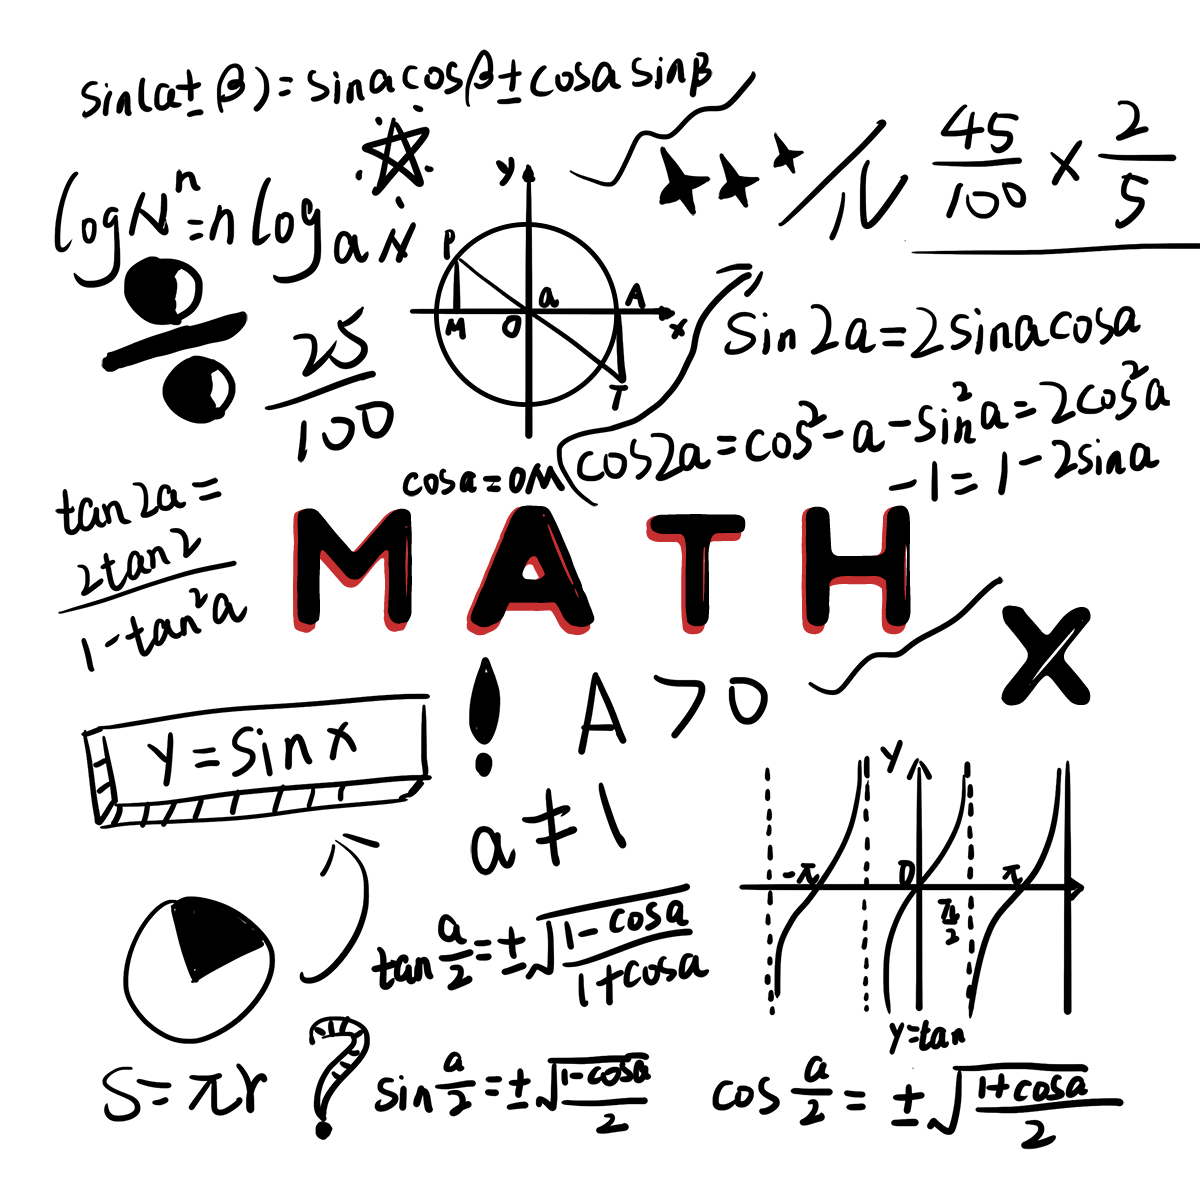
\includegraphics[width=15cm,height=15cm]{figure/cover.png}};

\vfill

{\Large Brendan W. Sullivan【著】\\[0.5ex]}

{\Large Fisher Yv【译】\\}

\vfill

\end{center}

\frontmatter

\tableofcontents

\mainmatter

\part{学习数学思维}\label{part:Part One}

% !TeX root = ../../book.tex
\chapter{什么是数学?}\label{ch:chapter01}

% !TeX root = ../../../book.tex
\section{真理与证明}\label{sec:section1.1}

你怎么知道一件事是真还是假?比如,上学时老师告诉你三角形的内角和为 $180$ 度,但你怎么\emph{知道}这是真的呢?万一你遇到一个从来没有学过基础几何的外星人呢?你如何\emph{说服}他/她/它相信这是真的呢?从某种程度上说,这就是数学:设计新的陈述,以某种方式确定它们是真还是假,并向其他人(也可能是外星人)解释这些发现。不幸的是,似乎很多人认为数学家成天做的就是把大数乘在一起;但事实上,数学是一门更具创造性和写作基础的学科,而不是人们普遍认为的复杂算术。本书的目标之一就是让你相信这一事实,但这不是主要目标。本书的主要目标是向你揭示数学思维、解决问题和给出证明的真正意义,并教你如何完成这些事情,以及它们是多么的有趣!

顺便一提,你可能好奇``某事为真意味着什么''?要想全面讨论这个问题需要深入到哲学、心理学、或许还有语言学层面,我们不想太过深入其中。然而就数学而言,其主要思想是:\textbf{只有我们能够}\emph{证明}\textbf{某事}\emph{永远}\textbf{为真它才为真}。我们知道 $1+1=2$ 永远为真。无论是黑夜还是白天,该等式永远成立。(不过,你有没有想过如何证明这一事实?实际上证明这个问题非常困难!有本名为\emph{《数学原理》}的书从``第一性原理''出发,经过很多很多页论证才得出 $1+1=2$!)这或许与其他科学完全不同。如果我们进行 $10$ 次物理实验并且观测到相同的结果,我们是否可以断定它会\emph{永远}发生?要是我们做一百万次实验会怎样?十亿次呢?我们在什么时点真正给出了\emph{证明}?在数学上,反复实验不是可行的证明!我们需要找到一个论证来说明为什么这种现象总会发生。举个例子,数学中有个著名的未解难题叫\href{https://baike.baidu.com/item/哥德巴赫猜想/72364}{哥德巴赫猜想}。目前还不知道其是否正确,尽管我们已经通过计算机模拟验证到大约 $10^{18}$ 都是正确的。$10^{18}$ 是个\emph{巨大的}天文数字,但仍不足以证明猜想是\textbf{真}是\textbf{假}。你看到差别了吗?数学家喜欢\emph{证明}事实,而不是用一堆值去检验,检验值只要不是\emph{全部}就\emph{不能}构成证明。

% !TeX root = ../../../book.tex
\subsection{三角迷思}\label{sec:section1.1.1}

在讨论证明的目标及其重要性时,我们引入了\textbf{证明}的概念。那么,如何\emph{定义}证明?这实际上是一个颇具挑战的问题!为逐步阐明这一概念,我们将给出若干数学论证案例。建议你仔细阅读,并思考它们是否具有说服力。它们\emph{证明}了什么?它们正确吗?是否正确?是否易于理解?阅读后有何感受?请先独立思考形成观点,然后再参考我们的分析。

我们给出的数学论证都与三角形有关。具体来说,都涉及\textbf{毕达哥拉斯定理}。

\begin{theorem}[毕达哥拉斯定理] \label{thm:pythagorean}
    在直角三角形中,若两直角边长分别为 $a$ 和 $b$,斜边长为 $c$,则 $a^2+b^2=c^2$。
\end{theorem}

\begin{center}
    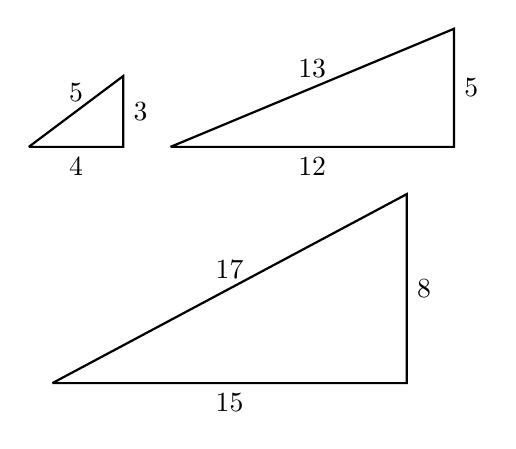
\begin{tikzpicture}[thick, scale=0.30]
        \draw (0,0) -- (4,0) node[midway,below]{$4$}
        -- (4,3) node[midway,right]{$3$}
        -- (0,0) node[midway,above]{$5$};
        \draw (6,0) -- (18,0) node[midway,below]{$12$}
        -- (18,5) node[midway,right]{$5$}
        -- (6,0) node[midway,above]{$13$};
        \draw (1,-10) -- (16,-10) node[midway,below]{$15$}
        -- (16,-2) node[midway,right]{$8$}
        -- (1,-10) node[midway,above]{$17$};
    \end{tikzpicture}
\end{center}

我们为何确信此定理成立?这个极其实用的结论,你可能在数学课堂上(或日常生活中不经意地)多次运用过。但你有没有思考过为什么这是真的?你会如何向持怀疑态度的朋友解释呢?这正是\textbf{数学证明}试图完成的:对事实给出清晰而严谨的解释。寻求证明背后的原因也十分有意义,它具有两重含义:即确保我们认为为真的事情确实为真,又避免要使用时进行重复论证。一旦(令人信服地)完成毕达哥拉斯定理的证明,后续只需引用定理名称即可;我们已经证明过了,所以无需再次证明。

那么,究竟什么构成了证明?如何判断解释是否足够清晰和简洁?一般来说,这些问题本身具有相当的复杂性,这也使得数学兼具科学与艺术的双重属性。尽管处理的都是严谨客观的事实,但如何有效地推理并以令人信服的方式呈现,实则是一门艺术。

\subsubsection*{``证明''范例}

让我们一起看几个``证明''的例子,看看它们是否足够好。(我们现在先说``证明'',稍后为其下更精确的定义。)这里是第一个:

\begin{proofs}{``证明'' 1.}
    构造边长为 $a+b$ 的正方形。在正方形内部放置 $4$ 个全等的直角三角形,形成边长为 $c$ 的内接正方形。

    \begin{center}
        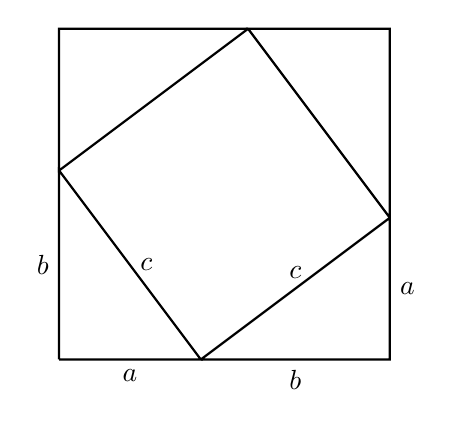
\begin{tikzpicture}[thick, scale=0.6]
            \draw (0,0) -- (3,0) node[midway,below]{$a$}
            -- (0,4) node[midway,right]{$c$}
            -- (0,0) node[midway,left]{$b$};
            \draw (3,0) -- (7,0) node[midway,below]{$b$}
            -- (7,3) node[midway,right]{$a$}
            -- (3,0) node[midway,above]{$c$};
            \draw (7,3) -- (7,7)
            -- (4,7)
            -- (7,3);
            \draw (4,7) -- (0,7)
            -- (0,4)
            -- (4,7);
        \end{tikzpicture}
    \end{center}

    大正方形的面积可以用两种方式表示:直接应用正方形的面积公式,或者把内接正方形和四个直角三角形的面积加起来。因此,下面这个等式一定成立。
    \[(a+b)^2=c^2+4\cdot\frac{ab}{2}=c^2+2ab\] 
    将左边表达式展开,然后两边同时消掉同类项可得 
    \[a^2+\cancel{2ab}+b^2=c^2+\cancel{2ab}\] 
    所以,$a^2+b^2=c^2$ 成立。
\end{proofs}

上面的证明是否具有说服力?每一步是否合理?可能你现在还太不确定,那么让我们接着看一下此定理的另一种``证明''。

\begin{proofs}{``证明'' 2.}
    假设毕达哥拉斯定理成立。绘制直角三角形,并过直角顶点向对应边做高。如下图所示:
    \begin{center}
        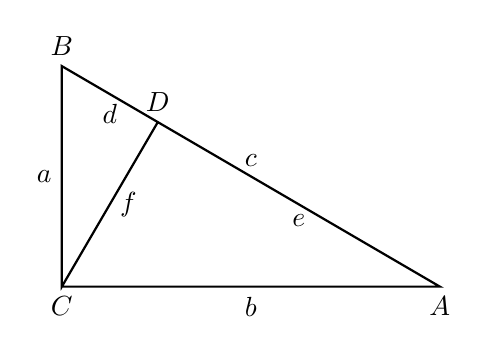
\begin{tikzpicture}[thick, scale=0.8]
            \coordinate (C) at (0,0);
            \coordinate (A) at (6,0);
            \coordinate (B) at (0,3.5);
            \coordinate (D) at (1.523316, 2.611399);
            \draw (C) node[anchor=north]{$C$}
            -- (A) node[anchor=north]{$A$} node[midway,below]{$b$} 
            -- (B) node[anchor=south]{$B$} node[midway,above]{$c$}
            -- (C) node[midway,left]{$a$}
            -- (D) node[anchor=south]{$D$} node[midway,right]{$f$}
            -- (A) node[midway,below]{$e$} 
            -- (D)
            -- (B) node[midway,below]{$d$};
            \rightAngle{B}{D}{C}{0.3};
        \end{tikzpicture}
    \end{center}
    因为毕达哥拉斯定理成立,所以我们可以将其应用到图中的三个直角三角形中,即三角形 $ABC, BCD, ACD$。(定义 $e = c-d$)可得
    \begin{align*}
        a^2 &= d^2 + f^2 \\
        b^2 &= f^2 + e^2 \\
        c^2 &= a^2 + b^2
    \end{align*}
    将前两个方程相加,再用代入第三个方程,可得
    \[c^2 = d^2 + e^2 +2f^2\]
    注意到 $\angle ABC$ 与 $\angle ACD$ 相等,因为它们都与角 $\angle CAB$ 互余,由此可知 $\triangle CDB$ 与 $\triangle ADC$ 相似。(此处默认你对平面几何有所了解。)由此可得 $\frac{e}{f} = \frac{f}{d}$,因此 $f^2 = ed$。我们可以将其带入上面的公式替换 $f^2$,结果如下:
    \[c^2 = d^2+e^2+2de = (d+e)^2\]
    两边同时开方(已知 $c,d,e$ 都是正数)可得 $c = d+e$,根据边长 $d$ 和 $e$ 的定义,这显然成立。因此,假设毕达哥拉斯定理成立是正确的。
\end{proofs}

这个证明怎么样?有说服力吗?表述清晰吗?在确定什么构成``正确的''或``良好的''证明之前,让我们再考察一个``证明''。

\newpage

\begin{proofs}{``证明'' 3.}
    观察下图
    \begin{center}
        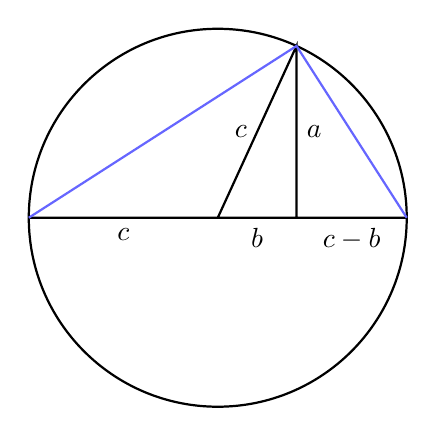
\begin{tikzpicture}[thick, scale=0.4]
            \coordinate (O) at (0,0);
            \coordinate (A) at (-6,0);
            \coordinate (B) at (6,0);
            \coordinate (C) at (2.5,0);
            \coordinate (D) at (2.5,5.45435);
            \draw (O) circle (6);
            \draw (A) -- (O) node[midway,below]{$c$}
            -- (C) node[midway,below]{$b$}
            -- (B) node[midway,below]{$c-b$}
            -- (C)
            -- (D) node[midway,right]{$a$}
            -- (O) node[midway,left]{$c$};
            \draw[color=blue!60] (A) -- (D) -- (B);
            \rightAngle{B}{C}{D}{0.6};
        \end{tikzpicture}
    \end{center}  
    由图形可得 $\frac{a}{b+c} = \frac{c-b}{a}$,因此 $a^2 + b^2 = c^2$。
\end{proofs}

这个证明对你来说合理吗?最后,还有一个需要思考的``证明''。

\begin{proofs}{``证明'' 4.}
    毕达哥拉斯定理必然成立,否则我的老师一直在欺骗我。
\end{proofs} 

\subsubsection*{讨论}

在继续阅读之前,建议你先独立思考这四个``证明'',也可与同学或朋友讨论一下。你认为什么构成``正确''的证明?清晰性和易读性重要吗?它会影响证明的``正确性''吗?

从历史角度看,数学证明的撰写历经多年演变,已经对什么构成``正确''的证明形成了普遍共识:

\begin{itemize}
    \item 从数学角度来说,证明中的每一\emph{步}、每一个逻辑推理和命题均需保持\emph{数学有效性},这一点非常重要。
    \item 同样重要的是,证明撰写者需(合理地)阐明陈述如何源于前置工作或外部知识。
\end{itemize}

这种对\emph{真理性}的要求,使得已建立的数学论证,可以通过逐步验证确认每个命题是\textbf{对}还是\textbf{错}。难点在于对清晰表达的界定。某种程度上,这就像最高法院大法官波特·斯图尔特(Justice Potter Stewart)对淫秽的著名定义:``见之即明''。

下面从清晰性和正确性两方面评估这四个论证:

\textbf{清晰性:}

\begin{itemize}
    \item ``证明'' 1 和``证明'' 2 表述清晰。明确解释了操作动机与依据。不仅给出了每个方程式的来源,还辅以图示说明。
    
    请注意,``证明'' 1 确实依赖一些基本的先验知识,例如基本代数运算以及三角形和正方形的面积公式,但这没有问题。

    同样地,``证明'' 2 依赖相似三角形的一些知识以及它们边长之间的关系。撰写者明确指出了这一点,所以有兴趣的读者可以查阅相关知识点。如果撰写者没有指出,读者可能会感到困惑,不知道如何得出这个结论。
    \item ``证明'' 3 写得非常糟糕!它没有提供任何解释。这使得读者很难确定其结论是否正确。尽管其中包括一张图片,但并没有解释\emph{为什么}要画一个三角形的外接圆,或者为什么能从图中得出所述方程。
    \item ``证明'' 4 虽语法正确,但并未提供任何\emph{解释}!
\end{itemize}

由此可见,对于一个逻辑正确且书写良好的证明来说,``证明'' 4 无疑是一个糟糕的证明。``证明'' 1 和``证明'' 2 仍在候选之列,因为它们至少写得很清楚。``证明'' 3 目前看可能不是一个好的证明;也许它确实包含正确的结论,只是需要更好的解释。通过重写可以使其变成一个良好的\emph{证明}。

让我们再来分析一下这四个论证的逻辑正确性:

\textbf{正确性:}

\begin{itemize}
    \item ``证明'' 1 大部分都很好。正确应用了正方形和三角形的面积公式,并且其代数运算也正确。但是我们怎么知道其所描述的过程 —— 将给定四个三角形放入正方形内 —— 会构建一个边长为 $c$ 的内接正方形?证明中只是说这样\emph{可以},但并未真正说明\emph{为什么可以}。不过,除此疏漏外,这个证明写得很好而且是正确的。
    
    (你能证明里面的形状实际上是正方形吗?看一下它的角度:你能说明为什么它们都是直角吗?)
    \item 很遗憾,``证明'' 2 完全是错误的!尽管它所做的每一个逻辑步骤都遵循前一个步骤。例如,假设我们以这种方式设置三角形,我们可以正确推断出 $\triangle CDB$ 和 $\triangle ADC$ 是相似三角形。然而,为什么我们可以在一开始就\emph{假设}该定理为\textbf{真}呢?总的来说,这不正是我们在证明中试图实现的目标吗?这是一个关键缺陷。\textbf{假设一个事实并从中推断出某些结论为真并不能得出原始假设必然为真。}
    
    如果这种方法有效,我们可以``证明''任意命题!举个例子:你如何看待以下证明 $0 = 1$ 的``证明''?
    \begin{proof}
        假设 $0 = 1$。那么,根据 $=$ 的对称性,$1 = 0$ 也是成立的。将这两个方程相加可得 $1 = 1$,这显然为真。因此,$0 = 1$ 是一个有效的假设,因此它一定为真。
    \end{proof}
    你看出上面证明与``证明'' 2 有什么相似之处吗?它们使用了同样有缺陷的推理:假设一个事实,做了一些工作得到我们已知为真的其他事实,然后断言假设的事实也必然为真。
    \item 对于``证明'' 3 ,大多数数学家会说这是一个``糟糕的证明'',尽管其透露出的结论似乎都是正确的。我们说``透露出''是因为,如果没有任何文字解释思路,就无从知晓撰写者想表达什么!然而,不得不说,完美证明的核心思路就包含其中。
    
    从图中,你可以证明方程 $\frac{a}{c+b} = \frac{c-b}{a}$ 一定成立。(提示:使用相似三角形!)进而可以推导出 $a^2 + b^2 = c^2$。

    你能写一些文字来配合图形,将其改写为良好的证明吗?
    \item 最后,几乎每个逻辑正常的人(我们希望如此!)都会说``证明'' 4 根本不是一个证明,无论做出这样的陈述多么方便。
\end{itemize}

综上,``证明'' 1 是一个良好的证明。在 4 个证明中,``证明'' 1 写得最清楚,逻辑也最正确。我们可以将其视作\textbf{证明}。``证明'' 2 是完全错误的,尽管它表述得非常清楚。``证明'' 3 包含正确的思路,但缺乏清晰的表述。``证明'' 4 离证明十万八千里,毫无讨论价值。

\subsubsection*{问题}

在继续讨论其他主题之前,留下一个问题供你思考:给定三个正数 $a,b,c$ 满足 $a^2+b^2=c^2$,是否一定存直角边长为 $a,b$ 斜边长为 $c$ 的直角三角形?倘若存在,你会如何着手构造它?若不存在,原因何在?


% !TeX root = ../../../book.tex
\subsection{质数时间}\label{sec:section1.1.2}

当我们讨论证明这个主题时,让我们看一下另一个重要定理的证明。首先简要回顾\emph{质数}的定义。

\subsubsection*{定义、示例与应用}

\begin{definition}\label{def:prime}
    若正整数 $p>1$ 的正因子只有 $1$ 和 $p$ 本身,则称 $p$ 为\dotuline{质数}。非质正整数称为\dotuline{合数}。
\end{definition}

质数在数学的诸多分支中都具有核心地位,而不仅限于研究整数性质的\textbf{数论}领域。数学中最著名的\textbf{猜想}(迄今为止既没有被证明也没有被证伪的命题)当数\emph{黎曼猜想}。该猜想已被证实与质数在整数中的分布规律密切相关,相关研究著作浩如烟海。此外,大多数现代密码学的基础都是大质数的乘积特性 —— 将两个大质数相乘容易,但将乘积逆向分解为两个大质数却极为困难。现在你知道了:每当你用信用卡在 iTunes 上购买歌曲时,背后的计算机系统都会将两个大质数相乘!

前几个质数依次为 $2, 3, 5, 7, 11, 13, 17, 19, 23,\dots$(注意,$1$ 不满足定义)。那么质数有多少个?相邻质数相距多远?是否存在分布规律?这些问题虽引人入胜却极难解答(有时甚至是不可能的!)。本节将聚焦其中一个问题:质数是否有无穷多个?

\subsubsection*{定理与证明}

\begin{theorem}[质数无穷性]
    质数有无穷多个。
\end{theorem}

\begin{proof}
    假设质数有有限多个,按升序列出为:$p_1, p_2, p_3, \dots, p_k$,所以 $p_k$ 为最大质数。现构造新数
    \[N = (p_1 \cdot p_2 \cdot p_3 \cdot \dots \cdot p_k) + 1\]
    $N$ 必有质因子。然而,它一定不能被 $p_1$ 或 $p_2$ 或 $\dots$ 或 $p_k$ 整除,因为根据 $N$ 的定义,除以上述质数都会得到余数 $1$。因此 $N$ 可以被列表中未列出的其他质数整除。

    如果 $N$ 是合数,那么我们就发现了一些新质数 $p < N$,它不在所有质数列表中。
    
    如果 $N$ 是质数,那么我们就得到了一个新质数 $N > p_k$,所以 $p_k$ 实际上并不是最大的质数。无论哪种情况,我们必然有一个新的质数不在给定的 $k$ 个质数的列表中,这与有限性假设矛盾。因此,质数必定有无穷多个。
\end{proof}

对于这个``证明''你怎么看?是否令你信服?这里的论证方式与我们迄今为止看到的其他论证方法有所不同。不妨尝试向同学解释本节的证明与上一节毕达哥拉斯定理的``证明 1''有何不同。我们很快将揭示:此处的``证明''实际上是一个完全正确的\emph{证明}!


% !TeX root = ../../../book.tex
\subsection{无理取闹}

现在让我们讨论另一类数字:\textbf{有理数}。你可能知道``分数''、``商''或``比率''指的都是有理数。

\subsubsection*{定义与示例}

以下是\emph{有理数}的精确定义:

\begin{definition}
    实数 $r$ 是\dotuline{有理数}当且仅当它可以表示为两个整数之比 $r = \frac{a}{b}$,其中 $a$ 和 $b$ 均为整数(且 $b \ne 0$)。

    一个实数不是有理数就是\dotuline{无理数}。
\end{definition}

定义并未规定有理数必须具有唯一的表示形式;它只要求有理数至少有一种定义中的表示。例如,$1.5$ 是有理数,因为 $1.5 = \frac{3}{2} = \frac{12}{8} = \frac{30}{20}$ 等等。这一定义具有完备性:一个实数不是有理数就是\textbf{无理数},\emph{非}有理数,即不存在将其表示为整数之比的形式。你可能知道 $\sqrt{2}$ 是一个无理数,但如何\emph{证明}这一点呢?请尝试自行证明。我们稍后会重新讨论这个问题(见示例 \ref{sec:section4.9.4})。其他常见的无理数还包括 $e, \pi, \varphi$ 以及 $\sqrt{n}$(其中 $n$ 为正整数且不为完全平方数)。

\subsubsection*{问题}

基于有理数/无理数的定义,我们可以探讨无理数的组合能否产生有理数。请尝试独立解答以下问题:若答案为``是'',请举例说明;若答案为``否'',请解释其不可能性。

\begin{enumerate}
    \item 是否存在无理数 $a$ 和 $b$ 使得 $a \cdot b$ 为有理数?
    \item 是否存在无理数 $a$ 和 $b$ 使得 $a + b$ 为有理数?
    \item 是否存在无理数 $a$ 和 $b$ 使得 $a^b$ 为有理数?
\end{enumerate}

你能构造出具体例子吗?事实上,这三个问题的答案均为``是''!前两问较为简单,第三问则略微棘手。

以下我们给出第三问的证明。有趣的是,该证明并不直接给出满足条件的 $a$ 和 $b$;而是将可能性缩小至两种情形,并证明其中\emph{必有}一种成立。听起来很有趣,对吧?我们来试试吧。

\begin{proof}
    已知 $\sqrt{2}$ 为无理数。考虑数字 $x = \sqrt{2}^{\sqrt{2}}$。有两种可能的情况:
    \begin{itemize}
        \item 若 $x$ 为有理数,则令 $a = \sqrt{2}, b = \sqrt{2}$ 即满足条件。
        \item 若 $x$ 为无理数,则令 $a = \sqrt{2}^{\sqrt{2}}, b = \sqrt{2}$,此时
        \[a^b = \Bigg(\sqrt{2}^{\sqrt{2}}\Bigg)^{\sqrt{2}} = \Big(\sqrt{2}\Big)^{\sqrt{2} \cdot \sqrt{2}} = \Big(\sqrt{2}\Big)^2 = 2\]
        $2$ 为有理数。
    \end{itemize}
    无论何种情形,均可找到无理数 $a$ 和 $b$ 使得 $a^b$ 为有理数。因此,这样的数字对必然存在。
\end{proof}

你觉得这个证明怎么样?是否有说服力?它以明确的``是''回答了上面的第三问,但未指明具体\emph{哪一对} $a, b$ 是正确的,而是告诉我们其中必有一对满足。(事实证明 $\sqrt{2}^{\sqrt{2}}$ 确为无理数,但这一事实需要额外证明。)

还有很多其他具体例子可以回答这个问题。你能想出任何其他方法吗?(提示:尝试使用 $\log_{10}$ 函数……)


\newpage
% !TeX root = ../../../book.tex
\section{大罗洞观}\label{sec:section1.2}

% !TeX root = ../../../book.tex
\subsection{简单符号}

\subsubsection*{数学是门语言}

尽管看上去全是符号(那些写得密密麻麻的教科书所呈现的),但数学不仅仅是我们纸上所用符号的集合。英语基于一组固定的符号(字母表中的 26 个字母加上常见的标点符号,如句点、逗号和括号),但我们可以以特定的方式将这些符号组合在一起,并遵循一定的标准和约定,创作出有意义的单词、短语、句子、段落等;从本质上讲,英语和任何其他语言一样,通过符号集合以及组织这些符号的规则集合,来传达含义。同样的概念也适用于\emph{数学语言}:有一组符号和一组作用于这些符号的规则。

一个区别是,我们在数学中使用的符号集合可能相当大,具体取决于当前讨论的数学分支。数学结构多样性的一个重要部分是我们总是可以创建和定义要使用的新符号。通常,这样做只是为了使内容更简短、更易于阅读。

数学与其他语言之间的另一个主要区别是,我们仔细选择如何\emph{定义}我们的单词及其表达的概念。通常,数学家的大多数争论都围绕定义展开。这可能会令你感到惊讶;似乎数学家就证明和猜想进行辩论才更合理,甚至数学家居然会辩论都是一个新奇的想法!为新发现的概念选择正确的定义和术语是数学发现和阐述的重要组成部分,因为这有助于发现者/发明者向其他感兴趣的人解释他/她的想法。(没有这个过程,数学就不会进步,只是一群孤立的人试图自己发现真理。)

口语的情况与此类似,但似乎没有那么极端。例如,如果你对你的朋友说,``我饿了'',或者``我感觉有点饿了'',或者``天哪,我饿死了'',他们听到的基本上是相同的信息,并给出大致相同的回应。然而,在数学中,我们的定义要精确得多,并且不包含口语允许的细微差别。当然,这两种哲学各有优缺点,但在数学中,我们尽可能追求精确,因此我们希望我们的定义准确且稳定。尽管如此,我们可以掌控这些定义是什么!这就是为什么关于定义的争论在数学世界中如此普遍:为手头的概念选择正确的定义可以使未来使用这些概念的工作变得更加容易和方便。

\subsubsection*{恰当选择定义}

作为一个具体的例子,让我们回到上一节中看到的质数的定义\ref{def:prime}。它说的是:

\begin{definition}
    如果大于 $1$ 的正整数 $p$ 其正因子只有 $1$ 和 $p$,则称 $p$ 为\dotuline{质数}。非质正整数称为\dotuline{合数}。
\end{definition}

这个定义似乎没有什么问题,不是吗?也许你会用不同的措辞或更简洁的表达或使用不同的可变字母或其他,但最终的信息是相同的:质数是具有特定属性的某种类型的数字。而你选择写出该特定类型的数字是什么(大于 $1$ 的正整数)以及该属性是什么(没有除 $1$ 和它本身以外的正因子),你将获得等效的定义。

不过,这个定义背后存在一些微妙的问题:为什么它是那种特定类型的数字?为什么我们如此关心这个特殊的属性 --- 只能被 $1$ 和它本身整除?如果定义略有不同怎么办?事情真的会有那么大的改变吗?我们将用另一个问题来解决这些问题:你如何看待以下质数的替代定义?

\begin{definition}\label{def:prime2}
    如果小于 $-1$ 或大于 $1$ 的整数 $p$ 其正因子只有 $1$ 和 $p$,则称 $p$ 为\textbf{质数}。
\end{definition}

你注意到细微的差别了吗?所有符合之前``质数''定义的数字仍然符合这个定义,但现在负数也适用!具体来说,给定任意数字 $p$ 在旧定义下是质数,$-p$ 现在在新定义下也是质数。这是一个合理的想法吗?负质数有什么问题?

质数的第三个定义怎么样?

\begin{definition}\label{def:prime3}
    如果正整数 $p$ 的正因子只有 $1$ 和 $p$,则称 $p$ 为\textbf{质数}。
\end{definition}

(请记住,按照惯例,$0$ 既不是正数也不是负数。)现在,负数会超出范围,但 $1$ 符合此定义。这合理吗? $1$ 的唯一正因子是 $1$ 和...它本身,对吗?

这就是可能引发争论的地方:也许你不介意让 $1$ 成为质数,但你的朋友会强烈反对。好吧,如果没有确凿的理由,就没有办法说你们中任何一个都是错的,真的;你只是对术语做了不同的选择,它们都没有改变 $1$ 的唯一正因子是 $1$ 和它本身这一固有属性。类似地,请考虑一下:无论你称它们为凉鞋、拖鞋还是人字拖,事实仍然是这些类型的鞋子适合在海滩上穿。

然而,考虑到历史的后见之明和新的愿望,通常一个特定的定义被认为更加合适。未来,我们将研究质数分解,这是一种将每个(正)整数写为质数乘积的方法。例如,$15 = 3 \cdot 5$, $12 = 2 \cdot 2 \cdot 3 = 2^2 \cdot 3$ 和 $142857 = 33 \cdot 11 \cdot 13 \cdot 37$ 都是质因数分解。

这些因数分解也有一个特殊的性质:一般来说,正整数的质因数分解是\textbf{唯一的}!也就是说,只有一种方法可以将正整数写为质数的乘积(因为我们将因子的不同排序视为同一事物,所以 $105 = 3 \cdot 5 \cdot 7$ 和 $105 = 7 \cdot 3 \cdot 5$ 是相同的因数分解)。我们将使用上面给出的第一个定义严格证明这一点。如果我们使用第二个定义或第三个定义会怎么样?这种唯一性还存在吗? 为什么这种唯一性如此重要?最终,结论是,定义应该由逻辑和实用性驱动,并且这可能会随着时间的推移而改变并引发一些争论。

\subsubsection*{数学家的学习模式}

建立清晰准确的定义的另一个好处是你可以像思想者一样获取知识和理解;人类学习的一个主要方面涉及通过日常经验识别模式,接着将想法、概念、词语、事件与这些模式联系起来。然后,人们可以使用这些模式来预测抽象的想法、概念和事件并对其进行理论化。

例如,研究表明,人类婴儿最初缺乏\emph{物体存继性}概念,随着时间的推移逐渐发展起来。如果你给孩子看一个他们喜欢的彩色玩具,然后把它藏在纸箱下面,孩子不太明白这个玩具仍然存在,只是看不见了。他/她会表现得好像该物体不再存在一样。然而,在某些时候,我们知道这不是真的,我们视野之外的物体仍然存在。这究竟是如何发生的?也许是我们见识到许多此类事件的模式,其中一个物体``消失'',然后我们又找到它。

更好的例子可以在自然科学中找到,它们说明了模式识别和抽象思维的另一个方面,这是极其重要的,特别是在数学和科学领域。我们可以想象,尼安德特人不知何故知道,每当他们拿起一块岩石并将其保持在一定距离,然后松开时,岩石就会掉到地上。这种情况可能一次又一次地发生,所以他们``明白''这种现象是自然的必然产物。在发生足够多的事件之后,人们很可能明白这种情况总会发生,或者至少,任何没有发生的情况都会引起极大的困惑和恐惧。(正是这种情绪反应可能有助于解释火山爆发等罕见但强烈的事件如何导致古代文明将此类事件归咎于``神之愤怒'')。

对事件的观察并没有使史前人类进一步理解\emph{为什么}岩石总是会掉落到地面,或者能够\emph{解释}为什么它每次都必然发生。几千年后,人们才开始思考这种现象为何发生以及如何发生,更长时间之后,艾萨克·牛顿(Isaac Newton)最终提出了一个试图解释重力行为的模型(最终为此类现象命名)。有人说,即使是现在,我们仍然没有弄清楚它到底是如何运行的。(如果你好奇的话,可以上网搜索``循环量子引力''并尝试理解这一点)。

正是这种思维上的抽象飞跃 --- 从对某种模式的观察到对该模式的认识论理解 --- 从最好的意义上来说,是真正具有好奇心和智慧的思想家、真正的科学家的特征。你认为谁是更好的昆虫学家:贪婪的读者,他已经记住了世界上所有目前已知的甲虫种类,或者实验室科学家,他检查了多种物种,可以采集新标本并对其分类为甲虫还是非甲虫?这在某种程度上是一个引导性问题,但要点是:\emph{理解}定义及其背后的动机比简单地了解一堆满足某个定义的\emph{实例}要有益得多。

可以说,这对数学更为重要。你能想象一个数学家不知道质数是什么,只能凭记忆列出前 100 个质数并对此沾沾自喜吗?当然不是!数学研究的美妙、通用和魅力部分在于我们检查模式和现象,然后选择如何做出与这些模式相关的适当定义。然后,我们利用对这些模式的新理解来对其他模式和现象做出严格精确的预测。彻底理解定义或概念可以提高预测能力,并且比仅仅了解该定义/概念的示例更为有效。



% !TeX root = ../../../book.tex
\subsection{正确撰写}

数学的另一个有趣的方面是,尽管它本身就是一种语言,但我们依赖外部语言来传达我们所拥有的数学思想和见解。尝试在不使用任何单词的情况下重写我们之前看过的定义和证明。这很难,不是吗?因此,我们希望用来传达数学思想的书面语言遵循与我们所写的数学``句子''相同的标准:我们希望它们\emph{精确}、\emph{合乎逻辑}且\emph{清晰}。

现在,为这三个词下一个精确、合乎逻辑且清晰的定义本身就是一项艰巨的任务。然而,我们都认同理想的证明应该具备:

\begin{itemize}
    \item \textbf{精确性:}任何个体陈述都不应是不真实的或可以通过多种方式解释从而导致真相需要商榷;
    \item \textbf{逻辑性:}每一步都应遵循先前的步骤,并有适当的动机和解释;
    \item \textbf{清晰性:}步骤间应该用正确的语法连接和描述,帮助读者了解发生了什么。
\end{itemize}

让我们检视几个无视这些标准并且在某种程度上不符合我们迄今为止的证明定义的``证明''。

\subsubsection*{糟糕``证明''\#1}

首先,我们来一个 $1=2$ 的``证明'',我们知道这肯定有问题。你能找到哪里出错了吗?它违反了哪个标准?精确性、逻辑性还是清晰性?

\begin{proofs}{``证明''}
    假设有两个实数 $x$ 和 $y$,考虑如下等式:
    \begin{align*}
        x &= y \\
        x^2 &= xy &\text{两边同时乘以\ } y\\
        x^2-y^2 &= xy-y^2 &\text{两边同时减去\ } y^2\\
        (x+y)(x-y) &= y(x-y) &\text{因式分解} \\
        x + y &= y &\text{两边同时消去\ } (x-y)\\
        y + y &= y &\text{因为第一行给定\ } x=y\\ 
        2y &= y \\
        2 &= 1 &\text{两边同时除以\ } y
    \end{align*}
\end{proofs}

这里的问题在于\emph{精确性}。对第四行进行因式分解后,除以公因数 $(x - y)$ 即可得到第五行,这似乎既方便又明智;然而,第一行告诉我们 $x = y$,所以 $x-y = 0$,\textbf{除以零是不允许的}!使用变量 $x$ 和 $y$ 只是一种让你失去踪迹并掩盖除以零的方法。(说到这里,为什么不能除以零?你能想出一个合理的解释吗?从乘法的角度思考一下。)

\subsubsection*{糟糕``证明''\#2}

这是类似``事实''的另一个证明,即 $0 = 36$。

\begin{proofs}{``证明''}
    考虑方程 $x^2+y^2 = 25$。整理并分离 $x$ 可得
    \[x = \sqrt{25-y^2}\]
    两边加3再同时平方得
    \[(x+3)^2=\Big(3+\sqrt{25-y^2}\Big)^2\]
    请注意,$x = -3$ 和 $y = 4$ 是原方程的解,所以最终的方程也应该是成立的。将这组解代入 $x$ 和 $y$ 可得
    \[0 = (-3+3)^2 = (3+\sqrt{25-16})^2 = (3+3)^2 = 36\]
    因此,$0 = 36$。
\end{proofs}

到底发生了什么?你能发现不合逻辑的步骤吗?如果我们使用最后选择的变量 $x$ 和 $y$ 的特定值重写证明步骤,也许会有所帮助:

\begin{align*}
    (-3)^2+4^2 &= 25 \\
    -3 &= \sqrt{25-4^2} \\
    (-3+3)^2 &= \Big(3+\sqrt{25-4^2}\Big)^2 \\
    0 &= 36
\end{align*}

现在很明显了,不是吗?对方程两边取平方根存在一个问题,它取决于 $(-x)^2=x^2$ 这一事实。

当我们解 $z^2=x^2$ 这样的方程时,必须牢记这个方程有两个根:$z = -x$ 和 $z = x$。因此,从方程开始并对两边进行平方是一个完全合乎逻辑的步骤(所得方程的真值与原方程的真值\emph{一致}),但反之却是一个不合逻辑的步骤(平方方程成立并不\emph{一定}等于平方根方程也成立)。这是一个带有\textbf{条件陈述}或\textbf{逻辑蕴涵}的问题,我们稍后会详细讨论这些概念(第 4.5.3 节)。现在,我们可以用下面的代码来总结这个概念:
\[\text{如果\ } a=b, \text{则\ } a^2=b^2, \text{反过来,如果\ } a^2=b^2, \text{则\ } a=b \text{\ 或\ } a=-b\]

这说明了为什么在上面``证明''中从 $x^2+y^2 = 25$ 到 $x = \sqrt{25-y^2}$ 这步是不合逻辑的:当有两种可能的选择时,我们立即假设平方根的一种特定选择。如果我们选择负平方根,会发生什么?试着将第二步替换为 $-x = \sqrt{25-y^2}$ 并重写证明,在最后对 $x$ 和 $y$ 使用相同的值。发生了什么? 如果你用 $x = 3, y = -4$ 代替呢?或者 $x=-5, y=0$ 呢?你能描述一下如何确定何时应该使用正根 $x$ 何时应该使用负根 $-x$ 吗?

\subsubsection*{数学使用``兼或''}

既然``或''这个词已经出现,我们先提一下上面句子中\emph{或}的使用。当我们说 ``$a = b$ 或 $a = -b$'' 时,我们的意思是,这两个陈述中\emph{至少}有一个必须为真,甚至可能两者都为真。现在,如果 $a \ne 0$ 且 $b \ne 0$,则只有其中一种结论性陈述可以为真;也就是说,在这种情况下,只有一个根(正或负)是正确的,而不是两者都是正确的。然而,如果 $b = 0$,那么两个结论性陈述说的是同样的事情,$a = 0$,因此规定\emph{或}意味着只有一个陈述可以为真并且不允许它们都为真,这是不合逻辑的。在其他情况下,这种区别会产生更显着的差异。

例如,如果你在餐厅点了一份三明治,服务员问:``您想要薯条还是土豆沙拉?'',这可以理解为,你可以选择其中一项,但不能同时选择两者。这就是\textbf{异或}的示例,因为它阻止你选择两个选项。或者,如果你忘记带书写工具去课堂,准备用老方法记笔记于是询问你的朋友,``我可以借用您的铅笔或钢笔吗?'',这可以理解为,你实际上并不关心提供两个选项中的哪一个,只要至少有一个可用即可。也许你的朋友两者都有,而且其中任何一个都可以。这是\textbf{兼或}的示例,并且这是所有数学示例中假定的解释。

\subsubsection*{不清楚的论证}

最后两个糟糕的``证明''问题在于精确性和逻辑正确性。我们要求良好证明的第三个条件是\emph{清晰}:我们希望文字能够解释证明者在每个步骤中完成的工作以及为什么该工作是相关的。换句话说,我们不希望读者在任何时候停下来问:``这句话是什么意思?''或``那是从哪里来的?''或因困惑而产生的类似问题。如果有帮助的话,考虑写一个证明,向你班上的朋友、将要阅读你作业的评分者或智力相当的家庭成员解释它。重读你自己写的证明,并尝试预测可能出现的问题或可能要求你进行的澄清,然后通过重写来解决这些问题。

证明可能因为多种原因失败或不清晰,首当其冲的是,单词和句子可能无法正确解释证明的步骤和动机,这实际上可能是因为单词太多(使读者负担过重而模糊了证明)或因为单词太少(没有给读到者足够的信息)或者因为所选的词语令人困惑(没有正确解释证明)。这些是证明\emph{语言}的问题。

从数学上讲,就清晰性而言,可能会出现许多问题。也许证明撰写者突然引入一个变量,但没有说明它是什么类型的数字(整数、实数等),或者跳过几个算术/代数步骤,或者使用新的符号而没有提前定义它的含义...这些行为在技术上都没有错误或不合逻辑,但它们肯定会给读者带来困惑。你能想到其他原因让证明不明确吗?尝试想出一种基于语言的原因和一种基于数学的原因。

\subsubsection*{糟糕``证明''\#3}

让我们陈述一个关于多项式函数的简单事实,然后查阅关于该事实的``证明''。仔细阅读论证并尝试找出一些不清楚的句子或数学步骤。

\textbf{事实:}考虑多项式函数 $f(x) = x^4-8x^2+16$。对于任意 $x$,该函数都满足 $f(x) \ge 0$。

\begin{proofs}{``证明''}
    无论 $x$ 的值是多少,我们将其代入 $x$ 的函数 $f$ 中,都可以通过对多项式进行因式分解写出该函数的输出值,如下所示:
    \[f(x) = x^4-8x^2+16 = (x-2)^2(x+2)^2\]
    而任意数字 $z$ 一定要么小于 $-2$,要么大于 $2$,要么严格介于 $-2$ 和 $2$ 之间,要么等于其中之一。当 $z > 2$ 时, $z - 2$ 和 $z + 2$ 都大于 $0$,因此 $f(z) > 0$。当 $z < -2$ 时,两项都为负而负数的平方为正,所以 $f(z) > 0$。当 $-2 < z < 2$ 时,类似情况再次发生,当 $x = 2$ 或 $x = -2$ 时,其中一项为 $0$,所以 $f = 0$。因此,我们要证明的必然成立。
\end{proofs}

这个证明有什么可批评的地方呢?首先,它正确吗?精确吗?符合逻辑吗?清楚吗?哪里不清楚?试着找出那些有点不清楚的陈述,无论是语言上的还是数学上的,并尝试适当地修改它们。在不指出个别错误的情况下,下面提供了上述事实的更好、更清晰的论证。

\begin{proof}
    我们首先对函数 $f(x)$ 进行因式分解,将其视为变量为 $x^2$ 的二次函数
    \[f(x) = (x^2)^2-8x^2+16 = (x^2-4)^2\]
    接下来,我们可以因式分解 $x^2-4=(x+2)(x-2)$ 并将原函数重写为
    \[f(x) = \big((x+2)(x-2)\big)^2 = (x+2)^2(x-2)^2\]
    对于任意实数 $x$,都有 $(x+2)^2 \ge 0$ 且 $(x-2)^2 \ge 0$,因为平方结果一定非负。两个非负项的成绩依然非负,所以 对于任意实数 $x$, $f(x) = (x+2)^2(x-2)^2 \ge 0$。
\end{proof}

第一个``证明''和第二个``证明''有什么区别?你重写的证明也像第二个证明吗?

对第一个``证明''的批评之一是它没有完全解释 $-2 < x < 2$ 的情况;相反,它只是说发生了``类似''的事情,并没有实际执行任何细节。这是数学中的常见情况(证明的某些步骤``留给读者''),这是一种简便技巧,有时可以避免繁琐的算术/代数,并使阅读证明更容易、更快速、更愉悦。但是,要谨慎使用该技巧。作为证明撰写者,确保步骤确实有效非常重要,即使你不打算在证明中呈现它们;你应该向读者提供简短的摘要或提示,说明这些步骤实际上是如何运作的。此外,证明撰写者应尽量不要在对证明最终结果至关重要的步骤上使用此技巧。

在上面的特例中,完全跳过了因式分解的实际步骤,并且只是顺便提及了对 $-2 < x < 2$ 情况的分析,但这些都是证明的重要组成部分!从任何维度上来说,这都是一个简短的证明,展示这些步骤并不代表在简洁性或清晰性方面做出了巨大的牺牲。这再次呼应了证明撰写既是科学也是艺术的观点:选择何时将一些细节验证留给读者可能很棘手。 在这种特殊情况下,展示所有步骤很重要。

尽管如此,我们给出的第二个证明要清楚得多。而且,完全摒弃了第一个``证明''中采用的分情况讨论技术!第一个``证明''中的一个情况存在清晰性问题,但我们没有简单地在重写版本中阐述细节,而是选择完全放弃该技术并使用更简短、更直接的证明。这并不是说第一个证明的技术是错误的。如果我们填补第一个``证明''论证中的空白,我们就会得到一个完全正确的证明。然而,该技术中的一些步骤是多余的。请注意,实际上 $-2 < x < 2$ 和 $x > 2$ 的情况在某种意义上是相同的:在这两种情况下,因子都满足 $(x - 2)^2 > 0$ 和 $(x + 2)^2 > 0$。事实上,第一种情况 $x<-2$ 也是如此!所以,当相同的最终观察结果对应于所有三个情况时,为什么要把论证分成三个不同情况呢?这种情况下,最好将它们合二为一(同样利用当 $x = 2$ 或 $x = -2$ 时,其中一个因子为 $0$ 的知识)。重申一遍,使用分开讨论技术当然没错。但是,它只会给证明增加不必要的长度。

我们在上面的段落中提到了术语``情况''和短语``分情况讨论'',但没有恰当定义或解释我们的意思。现在,我们想推迟对这些术语的讨论,直到我们在第 4 章中彻底讨论逻辑。不过,如果你渴望立即解决这个问题,可以跳到第 1.4.4 节并查看``匈牙利朋友''问题,其中包含一些复杂的分情况讨论。


% !TeX root = ../../../book.tex
\subsection{选择逻辑}

我们已经非常频繁地使用``逻辑''一词及其相关形式,但还没有充分解释其意思。我们意识到这似乎违背了我们迄今为止一直大力倡导的精确性和清晰性,但不幸的是,我们不得不承认,提供\emph{逻辑}的完整定义是极其困难的。

\subsubsection*{一场游戏}

如果你寻找对逻辑的启发式理解,可以尝试从``逻辑谜题''(如数独或数谜)入手来思考它。这些谜题/游戏从一开始就围绕定下的非常具体的规则构建的,然后向解谜者提供一个起始谜面,并期望解谜者严格遵守规则,直到解出谜题。例如,在数独中,规则是 1 到 9 中每个数字在每行、每列和 $3 \times 3$ 框中恰好只出现一次,解谜者需要综合各种情况在网格中放置越来越多的数字,不断缩小``潜在解''的范围,以找到起始谜面的唯一答案。这个解谜过程的一个重要方面是,任何时候都不要(自作聪明地)\emph{猜测};每一步都应该在考虑当前情况和谜题既定规则的情况下进行理性选择,并且在这个框架内,保证谜题是可以解决的(当然,要有足够的时间)。

数学逻辑在某些方面略有不同,但本质是一样的:都有既定的游戏规则,每一步都应该以这些规则和当前知识为指导,除此之外别无其他。这就是我们所说的撰写数学证明应该受\emph{逻辑}支配的意思:从一个真理到另一个真理,每一步都应该遵循约定的规则,并且只参考这些规则或已经证明的事实。我们在证明(以及一般的数学中)中玩的``游戏''或``谜题''并不像数独谜题那么清晰。然而,更令人困惑的是,有时我们会投身一场无法获胜的游戏,却丝毫没有意识到这一点!

这里``无法获胜的游戏''的想法来自 20 世纪奥地利逻辑学家、数学家库尔特·哥德尔 (Kurt Gödel) 的工作成果,这是一项令人震惊、使人惊奇但极其有力的结论。他的\emph{不完备性定理}反映出一个强大的逻辑系统内部的固有问题:有些\textbf{真实}陈述在该系统内却是不\emph{可证明}的。在这里,我们无法透彻详细地解释一些术语(即,\emph{逻辑系统}和\emph{可证明}),但希望你能看到这里出现了一些神奇的事情。这怎么可能呢?如果某事在数学中是\textbf{真的},我们不是应该能够以某种方式证明它是真的吗?否则我们怎么知道这是真的呢?

\subsubsection*{数学简史}

要回答这些自然而生的问题,让我们先退一步,回到数学的一个重要分支 --- 逻辑的起源进行讨论。在整个讨论过程中要记住的一点是,我们无法完全解决出现的每个主题,这可能让人感到不满,我们理解这一点。数学之美部分在于,学习任何一个主题都会带来许多其他问题和概念需要思考,而这些问题和概念又可以通过更多的数学来解决。不过,背景很重要,就本书的背景而言,我们没有足够的时间和空间去讨论所有这些相关的主题。我们并不是试图向你隐瞒任何事情或掩盖某些问题;相反,我们只是在面对现实,确保我们不会强迫你阅读 10,000 页的完整数学史,只是为了理解我们的观点!

在你的数学生涯中,可能会进一步研究我们下面提到的许多数学家(以及他们所做的工作)。到那时,你将通过亲自动手实践从而对这个学科有更深入的理解和欣赏,你也将更有能力去解决其中的问题。而现在,我们仅仅是基于兴趣介绍这些数学家。数学有着丰富而有趣的历史,了解它会很有帮助!在这里,我们将尽力以简洁而有意义的方式来解读逻辑学 --- 它的历史、动机和意义 --- 使之与当前的背景相契合。

19 世纪中后期的数学家和哲学家首先研究了后来演变成现代逻辑的思想,他们对我们在这里试图研究的许多相同问题感兴趣:我们如何知道某件事是\textbf{真}的?我们如何才能表达这个真理呢?我们可以声明什么类型的``事件''为\textbf{真}或为假?这些数学家从根本上分解了数学语言,研究了如何以非常具体的方式组合一组固定的符号来创建更复杂的陈述,但从总体上看,这些陈述仍相当简单。这并不是要贬低他们的努力,毕竟,我们都必须从某个地方开始,而这些人是从头开始的。

首先进行的一项重大工作是探究算术的基础,或者说\textbf{自然数}($1,2,3,4,\dots$)的研究。就像欧几里得(Euclid)研究几何时,先通过建立一系列公认的真理或\textbf{公理},然后从这些给定的假设中推导出真理一样,意大利数学家朱塞佩·皮亚诺(Giuseppe Peano)建立了一套自然数公理,而其他人则从稍微不同的视角对这个主题进行了研究。与此同时,对真理及其证明严谨果断的欣赏,促使得大卫·希尔伯特和其他人提出了欧几里得公理的一些问题,尤其是平行公设。

这项关于几何和算术的工作自然引出了对数学其他领域的进一步、复杂的研究,以及对诸如实分析等领域热切地公理化尝试。卡尔·魏尔斯特拉斯(Karl Weierstrass)在研究这个主题时,提出了一些具有奇特属性的令人震惊的函数示例。例如,尝试定义一个处处不可微的连续函数。(如果你对微积分的这些术语不熟悉,请不用担心;总之,这很难。)最后,理查德·戴德金(Richard Dedekind)能够建立一个严谨的、逻辑的实数定义,完全由自然数推导出来,并且不依赖于必须存在数字连续体这种模糊的物理概念。

后来,这项研究稍微分支出来,变成了集合的研究。这个领域的许多基础工作是乔治·康托尔(Georg Cantor)在 19 世纪末期奠定的。他是第一个真正研究无限集理论的人,提出了无限有不同``大小''这一有争议的观点。也就是说,他证明了某些无限集严格大于其他无限集。这个想法在当时引起了极大的争议,以至于许多数学家都讨厌他!如今,我们意识到康托尔是对的。(这也让你提前窥探我们稍后在 7.6节中将会讨论的内容。举个有趣的例子:奇数集合和偶数集合当然一样大,但它们也和所有整数的集合一样大。然而,所有实数的集合严格大于二者!)

事实上,一些数学家对康托尔的发现感到相当震惊,甚至伟大的伯恩哈德·黎曼(Bernhard Riemann)一开始也认为集合论的发展将成为数学的祸害。但事实并非如此,从诞生起它就蓬勃发展,许多数学家致力于以正确的方式表示所有数学并理解数学的``基础''。某种程度上,你可以将集合论视为对所有数学家正在研究的基本对象的研究,最终,其方式类似于所有化学都是通过将元素周期表中的元素以越来越复杂的方式恰当地组合在一起来完成的。

这些主题的进一步发展是符号逻辑的研究,它比我们迄今为止提到的抽象概念更具体一些,而且我们在本书的开始章节中会频繁地研究这个领域的基本理念。该领域涵盖了如何将数学方程和符号与基于语言的符号和连词结合起来,以做出有意义的数学陈述,并可以通过证明来确认这些陈述的真实性。总的来说,这是数学的一个极其重要的组成部分,尤其是本书。个人观点当然比这更加细致和具体,但总的来说,大多数数学家的心态是,有许多数学真理等待被发现,我们花时间学习我们已经发现的真理,希望揭示更多真理。这就像一个巨大的考古挖掘,研究我们已经出土的骨头和文物将帮助我们预测我们在什么地方会发现什么类型的其他宝藏,以及如何寻找和挖掘。某种程度上,逻辑是从挖掘中一步一步抽象出来的过程:逻辑是对挖掘过程的研究。 它告诉我们如何真正利用数学知识并从中学习,并将其与其他知识相结合,从而证明更多的真理。

请注意,这不是一个精确的类比,抽象逻辑的研究要复杂得多。不过,就本书的目的而言,这是一种合理的思考逻辑的方式。我们将学习符号逻辑的一些基本原理和基本运算,并将这些知识应用到我们撰写证明的研究中。它将帮助我们真正理解证明是什么,它将指导我们构建要编写的证明,它将允许我们批判可能不正确的证明,并最终帮助我们理解数学作为一个整体是如何工作的。

\subsubsection*{逻辑应用:理论计算机科学}

逻辑思想和结果的一个非常重要的应用是计算机科学的发展和研究,特别是理论计算机科学和可计算性理论。这个特殊的数学分支最初是受大卫·希尔伯特二十三个问题 --- 1900 年出版的数学界著名未解决猜想列表 --- 中的第十个问题推动的。第十问题涉及解\textbf{丢番图方程(Diophantine Equations)}, 就是以下形式的方程
\[a_1x_1^{p_1}+a_2x_2^{p_2}+a_3x_3^{p_3}+\dots+a_nx_n^{p_n} = c\]
其中 $a_1, a_2, \dots, a_n$ 和 $c$ 都是给定的常数,$p_1, \dots, p_n$ 为给定的自然数,$x_1, \dots, x_n$ 为要求的使方程成立的变量。

给定这样一个方程,人们可能想知道是否存在解,如果存在,那么存在多少组解。 此外,如果我们给定常数 $a_i$ 和 $c$ 都是有理数,我们想知道是否可以确保存在一组解,其中所有变量 $x_i$ 也都是有理数。关于这个特定问题已经建立了一些理论成果,但是根据 1900 年的陈述,希尔伯特第十问题问的是,是否存在``一个过程,根据该过程可以经过有限数量的操作确定它''是否存在给定方程的解,其中所有变量 $x_i$ 都是有理数。尽管当时还没有算法这个术语的正确概念或定义,但希尔伯特要求的是一种\textbf{算法},该算法接受常数 $a_i$ 和 $c$ 的值,并根据是否存在所需属性的解输出 \textbf{True} 或 \textbf{False}。这个问题的一个重要部分是,该``过程''在输出答案之前执行有限数量的步骤。

一位名叫艾伦·图灵(Alan Turing)的英国剑桥大学学生几年后开始研究这个问题,他想到了一台物理机器,该机器将执行输出所提出问题的答案所需的步骤。他在随后的出版物中描述了他的发明,我们现在称之为\emph{图灵机},这是一种有趣的理论装置,可以用来回答形式逻辑中的一些问题,但也展现了构建现代计算机的许多想法。我们说它是一个理论装置,是因为它的定义的属性决定了它在物理上无法构建和操作,但它很好地处理了一些理论问题,包括前面提到的希尔伯特第十问题。更具体地说,当我们说某件事是可计算的,或者能够在有限数量的步骤中确定时,这台机器为我们的意思提供了正确的定义,这有助于建立正确的算法概念。如果我们在讨论可计算性话题时不提及阿隆佐·丘奇(Alonzo Church),那是不公平的,因为他与图灵同时在研究类似的问题。他们的名字一起出现在丘奇-图灵论文中,该论文将图灵机的工作原理与更理论化、基于形式逻辑的可计算性概念联系在一起。

\subsubsection*{我们将用逻辑做什么?}

虽然集合论和逻辑中的所有这些主题本质上都很有趣并且对数学非常重要,但总的来说,我们根本没有足够的时间和空间来详细讨论它们。相反,我们更关注在撰写和批判数学证明时使用的逻辑概念。

我们将考虑:

\begin{enumerate}
    \item 我们实际上可以陈述和证明什么类型的``事物'',
    \item 我们如何将我们已知为真的``事物''结合起来以产生更复杂的真理,
    \item 我们如何解释我们是怎样得出``事物''确实为真的结论。
\end{enumerate}

由于缺乏更好的术语,这里我们用``事物''一词,因为我们还没有\textbf{数学陈述}的正式定义,而这实际上是我们将要证明的``事物''的类型。从本质上讲,数学陈述是数学和语言中符号和句子的组合,可以验证为\textbf{真}或为\textbf{假},但不能同时既真又假或非真非假。那么,证明就相当于组织一系列步骤和解释,使用为真的数学陈述和句子将这些真理连接在一起,并最终产生特定陈述所需的真理。我们对逻辑的研究将解决如何组合这些步骤并确保我们的证明最终会导出对真理的正确评估。

更具体地说,我们将研究数学陈述到底是什么,以及如何将它们组合起来产生更复杂的陈述。``\emph{与}''和``\emph{或}''这两个词在其中特别重要,因为这两个词允许我们以新的、有意义的方式将两个数学陈述组合在一起。我们还将研究\textbf{条件}数学陈述,即``如果 A,则 B''或``A 蕴含 B''形式的语句。这些是数学陈述的基础,大多数重要的数学定理都是这种形式。这些陈述涉及做出一些\emph{假设(assumption)}或\emph{假说(hypothes)}(包含在陈述 A 中),并使用这些假设的事实得出结论(包含在陈述 B 中)。回顾 \ref{sec:section1.1.1} 节中毕达哥拉斯定理的陈述,注意它是如何以条件陈述的形式出现的。(可以用另一种方式书写吗?尝试以非条件形式重写定理的陈述,并思考在该形式下是否本质上是不同的陈述。找到另一个以条件陈述形式给出的著名数学定理,并尝试进行相同的格式更改。)

数学中的另一个重要思想,也是在证明撰写中经常出现的思想,是\textbf{变量}的概念。有时我们想笼统地讨论一种数学对象,而不为其分配特定的值,这就需要通过引入变量来实现。你可能在之前的数学学习中经常看到这种情况发生,甚至在本书中我们已经使用过变量了。再看看 \ref{sec:section1.1.1} 节中的毕达哥拉斯定理的陈述。字母 $a,b,c$ 代表什么?好吧,我们并没有给出明确说明,但我们知道它们是正实数,表示直角三角形三边的长度。什么三角形?我们并没有给出一个具体的三角形,也没有给出一张具体的图画或类似的东西,但你清除我们在说什么。此外,我们要检查的证明并不取决于这些变量的实际值,而仅仅取决于它们是否是具有某些属性的正实数。 这是非常有用且重要的,某种程度上,它节省了时间,因为我们不必单独考虑宇宙中所有可能的直角三角形(有无穷多个!) 并且可以将整个想法简化为一个紧凑的陈述和证明。

我们可以对变量进行\emph{量化}。这涉及到声明某个陈述对于变量的\emph{任意}潜在值或仅对\emph{某个}特定值是否成立。例如,在毕达哥拉斯定理中,我们不能声称 $a^2+b^2=c^2$ 对任意正实数 $a,b,c$ 成立;我们必须对变量施加额外的假设才能获得我们所做的结果。这是\textbf{全称}量化的一个例子:``对于\emph{所有}具有这个属性和那个属性的数字 $a,b,c$,我们可以保证...''同样地,我们还可以进行\textbf{存在}量化:``\emph{存在}一个具有此属性的数$n$。''

你能想到我们迄今为止已经研究过的使用存在量化的定理/事实吗?再来看一个证明,存在无理数 $a$ 和 $b$ 使得 $a^b$ 是有理数。请注意,我们证明的这个主张属于存在类型:我们声称\emph{存在}两个具有所需属性的数字,然后我们继续证明确实必然存在这样的数字。眼下,这个证明的有趣之处在于它是\emph{非构建性的};也就是说,我们能够在不明确给出数字 $a$ 和 $b$ 实际是什么的情况下证明我们的主张。我们将其缩小到两个选择,但从未声称哪一个是正确的选择,只是其中之一必然有效。


% !TeX root = ../../../book.tex
\subsection{明显的混淆}

作为这些逻辑概念的预览,我们将在稍后详细研究其数学细节,让我们举一些现实世界中基于语言的例子来说明这些想法。

\subsubsection*{条件陈述}

首先,让我们研究一下\textbf{条件陈述}。数学定理经常采用条件陈述的形式,但这种类型的陈述也经常出现在日常用语中,有时是隐含的(这只会增加混乱)。例如,人们有时会谈论他们将如何处理彩票奖金,比如
\[\text{如果我中了彩票,那么我就买辆新车。}\]
``那么(then)''之后的语句依赖于``如果(if)''相关的语句。当``如果(if)''部分的条件满足时,保证会发生``那么(then)''部分的操作。

条件语句中与``如果(if)''相关的部分称为\textbf{假说(hypothesis)}(更正式的名称为\textbf{先行词(antecedent)})。与``那么(then)''相关的部分称为\textbf{结论(conclusion)}(更正式的名称为\textbf{结果(consequent)})。

有时条件句的结论更加微妙,甚至句子中的动词时态不包含``如果(if)''。以电影《壮志凌云》中的台词为例:
\[\text{这是机密。我可以告诉你,但那样我就不得不杀了你。}\]
这里,第一部分``我可以告诉你''是一个伪装的假设。与实际电影台词具有相同逻辑含义的说法是``\emph{如果我告诉你,我就不得不杀了你}'';然而,这么说没有原台词富有戏剧性和张力。实际上,在条件陈述的结论中常常不包含``那么(then)''一词。在阅读句子时,你甚至可能不知不觉中在脑海里添加该词。下面是 The Barenaked Ladies 乐队的一首歌中的歌词:
\[\text{如果我有 100 万,我们就不必步行去商店了。}\]
\[\text{如果我有 100 万,我们会乘坐豪华轿车,因为它更贵。}\]
这两行都是条件陈述,但都不包含``那么(then)''一词;它被理解为句子的一部分。

将上述示例与以下句子进行比较,看看有什么不同:
\[\text{只有下雨的时候我才带伞。}\]
这里,说话人不愿意在没有正当理由的情况下随身携带雨伞,而是更愿意确保它有用。这句话与下面类似的句子意思相同吗?
\[\text{如果我带着雨伞,那就是下雨了。}\]
在现代语言用法中,条件的概念可能有点模糊。例如,第一句可以解释为有时可能下雨,但说话人忘记带伞。第二句是一个条件陈述的明确断言:看到我撑着伞走来,你一定会推断这是因为下雨了。在数学中,我们把这两个句子联系起来,说它们有相同的逻辑意义。

这引出了短语``仅当(only if)''的含义,以及随后的短语``\textbf{当且仅当(if and only if)}''。考虑以下两句话:
\[\text{如果中了彩票,我会买辆新车。}\]
\[\emph{只有}\text{中了彩票,我才会买辆新车。}\]
第一句说中彩票保证我会买辆新车,而第二句说买新车的行为保证是因为我刚刚中了彩票。如果这两句话都为真,那么``中彩票''和``买新车''这两个事件在某种意义上是等价的,因为其中一个事件的发生\emph{必然保证}另一个事件的发生。

因此,数学定义通常使用``\textbf{当且仅当}''这一短语。例如,我们可以写``一个整数是偶数,当且仅当它能被 $2$ 整除。''这表明知道一个数具有该性质可以称之为``偶数'',知道一个数是偶数可以得出其整除性质。(不过,有时一个定义只会使用\emph{当(if)},而\emph{仅当(only if)}部分没有说明但能被理解。你可能已经注意到,我们在 \ref{sec:section1.1.2} 节中对质数的定义就是这样做的。)

\subsubsection*{创建更多条件陈述}

从一个条件陈述开始,只要稍加修改,便能生成其他三个内容相同但结构不同的条件陈述。继续使用``彩票/汽车''的例子,让我们考虑原句的以下四个版本:

\begin{enumerate}
    \item 如果我中了彩票,那么我就买辆新车。
    \item 如果我买了辆新车,那么我中了彩票。
    \item 如果我中不了彩票,那么我就不会买新车。
    \item 如果我没有买新车,那么我就没中彩票。
\end{enumerate}

这些句子比较起来怎么样?它们中的任何一个都有相同的逻辑含义吗?假设第一个为真,那么所有这些都为真吗?我们认为,在这种情况下,即使第一句是真的,第二句也可能是假的。也许我在工作中得到了大幅加薪,或者继承了一笔钱,所以决定买辆新车。第三句和第四句呢?它们能以某种方式与其他句子联系在一起吗?这个就留给大家自己讨论和探索吧。对我们研究过的其他条件陈述提出同样的问题,看看你的答案是否也不同,这可能会很有趣。

最后一个条件陈述的例子来自脱口秀演员德米特里·马丁(Demetri Martin)的一个笑话。

\begin{quote}
    我走进一家服装店,一位女士走过来对我说:``如果你需要什么,我是吉尔。''\\我以前从未见过有条件身份的人。``如果我什么都不需要怎么办!你是谁?''
\end{quote}

上面的例子应该会让你体会到现代语言中条件陈述的不精确或微妙,有时需要进一步解释。在数学中,我们希望此类陈述是严格的、定义明确的且无歧义的。我们稍后将在第 \ref{sec:section4.5.3} 节中进一步研究这一点。不过,就目前而言,以计算机算法解释 \verb|if...then| 的严格方式来思考此类陈述可能会有所帮助。当 \verb|if| 部分的条件满足时,子程序被执行,否则被忽略。同样,\verb|while| 循环只是 \verb|if...then| 语句的序列,只是被压缩成一种简洁的形式。

\subsubsection*{量词}

接下来,让我们看一些量词的例子。当存在一个未知变量是从一组可能的值或表示中提取对象时,我们将使用量词。例如,当我们在毕达哥拉斯定理的陈述中量化变量 $a,b,c$ 时,它们是从表示直角三角形边长的实数集中提取的。对于非数学示例,请考虑以下句子:
\[\text{每个人都被某人爱着。}\]
这里有哪些变量?它们是如何量化的?请小心,因为这句话中实际上有两个量化,两个变量各一个。在这两种情况下,变量都代表世界上所有人集合中的成员,第一个变量是全称量化,而第二个变量是存在量化。这听起来可能令人困惑,所以让我们试着用更详细的措辞改写这个句子:
\[\text{对于世界上的每个人\ } x \text{,都存在另一个人\ } y \text{,具有\ } y \text{\ 爱\ } x \text{\ 的属性。}\]

你看出来这和第一句话的逻辑意义是一样的吗?当然,对于对话来说,这个内容有点过于冗长和精确,但我们在这里展示它是为了向你揭示潜在的变量和量词。量词的关键短语是``\emph{对于所有(for every)}''(全称量化)和``\emph{存在(there exists)}''(存在量化)。

\subsubsection*{量化顺序很重要!}

现在,让我们看一个与上面示例类似的句子:
\[\text{某人被每个人爱着。}\]
这句话和上面那句话很相似;甚至它们的用词都相同!词序变化对句子的逻辑意义有何影响?这里仍然有两个变量和两个量词,一个是全称量词,一个是存在量词,但是这些量词的应用顺序发生了改变。这句话的更详细表述是:
\[\text{存在某人\ } x \text{\ 具有对于世界上的每个人\ } y, y \text{\ 都爱\ } x \text{\ 的属性。}\]

这和第一句话的意思完全不同!第一个似乎可信,但这个就很奇怪。这个例子应该让你明白保持量化顺序是多么重要,这样你才能真正表达你的真实意思。

\subsubsection*{嵌套量词}

下面的例子说明我们的大脑在处理语言中的量词时有时是多么得快速和轻松,即使这种相互联系可能让人难以理解。当量词一个接一个地跟在后面时,我们称之为\emph{嵌套}。

分析和理解这些句子的能力可能取决于句子的上下文及其试图传达的信息。如果信息有意义并且我们相信它,那么它就更容易理解。关于这一现象,我们所知的最好的例子是伟大的总统演说家亚伯拉罕·林肯(Abraham Lincoln)的以下名言:

\begin{quotation}
    你可以一直愚弄一些人,有时也可以愚弄所有人,但你不能一直愚弄所有人。
\end{quotation}



这里到处都是量词!我们谈论的是所有人的集合,以及某些被愚弄人的集合,并对这些集合进行量化。尝试用几种不同的措辞重写这个句子,看看它是否听起来更``简单''或更简洁。是否存在另一种表达句子的方式,可以删除部分(或全部)量词而不改变含义?

最后,出于个人兴趣和幽默感,我们将引用鲍勃·迪伦(Bob Dylan)《Talkin World War III Blues》中的一句类似的话,这首歌来自鲍勃·迪伦 1963 年发行的专辑《The Freewheelin' Bob Dylan》:

\begin{quotation}
    \begin{tabular}{ll}
    Half of the people can be part right all of the time & 半人可常半对,\\
    Some of the people can be all right part of the time & 数人可暂全对。\\
    But all of the people can't be all right all of the time & 众人难恒皆对,\\
    I think Abraham Lincoln said that & 我思林肯所谓。
    \end{tabular}
\end{quotation}

稍后我们将更详细地讨论这些主题,那时我们将研究它们的数学动机、含义和用途。目前,我们再怎么强调这些问题在撰写证明中的重要性都不为过。把一堆句子串在一起,却不知道它们是如何连接的,这并不是证据,但一系列结构合理的逻辑陈述和含义才是我们真正想要的。

\newpage
% !TeX root = ../../../book.tex
\section{重审-重做-重生}\label{sec:section1.3}

到目前为止,我们一直试图从逻辑的角度激发和解释数学推理和证明撰写,但在此过程中,我们使用了一些你可能熟悉或不熟悉的数学概念和技术。当然,在研究数学时,逻辑和理性思考很重要,但这只是冰山一角。我们试图解释如何组织数学思想,并以一种有意义的方式构建它们,使其他人相信某个特定的事实,但这些思想必须包含与该事实相关的数学概念!

例如,如果没有对几何学的基本了解:三角形是什么,三角形、直线和角度的一些基本性质等等,我们就不可能看到毕达哥拉斯定理的任何证明。我们还假设读者理解什么?许多步骤都涉及算术,例如通过乘以相同因子或减去两个方程来处理多个方程,等等。这些想法现在可能是你的第二天性,但在某个时候你一定学习过这些东西,并了解它们为何以及如何实际发生作用,以便你将来可以安全且恰当地使用它们。

回顾一下前面几节中的证明。我们都用了什么数学思想?试着写下来,并思考你是何时以及如何了解它们的。尝试写下一些我们可能在没有明确说明的情况下使用的具体事实,并思考为什么我们要这样做。另外,试着找到一些我们提出主张但不一定完全解释为什么它一定\textbf{为真}的例子。例如,在毕达哥拉斯定理的 ``证明 1'' 中,我们在一个正方形内画了四个相同的三角形,然后说里面的图形也是一个正方形。这是\text{真}的吗?我们怎么能这么确定呢?尝试证明一下!

\subsubsection*{先验知识}

要点是,巧妇难为无米之炊,如果不注入一些有意义的数学内容,我们实际上就无法撰写证明。因此,本书的主要目标之一是与你分享一些有趣的数学事实。有时,这涉及使用你已经了解和以前见过的对象(例如三角形或质数)并尝试用它们做新的事情。有时,我们会向你介绍全新的数学对象(例如等价关系或二项式系数)并使用它们。现在,我们想做的是讨论一些我们将经常使用的数学对象和概念,这些对象和概念你可能以前见过。但我们不假设所有这些对象和概念你都见过,这些思想快速学习/重新学习起来都不太难,并且它们在本书的剩余部分以及你数学生涯的剩余部分非常有用!本节中和本节最后提供了一些问题供你解决,以便为你提供一些练习。

% !TeX root = ../../../book.tex
\subsection{速算}

我们不期望你心算六位数乘法或类似的事情,但是能够通过加法、减法和乘法来运算``小''数字是一项重要的技能。当然,计算器和计算机程序可能会有所帮助,但我们希望每当我们需要添加几个四位数字时,没有必要运行在 \verb|Maple| 或 \verb|Mathematica| 或 \verb|TI-89| 上。技术在准确性和时间效率上为我们提供了许多便利,但当我们过于依赖这些设备时,我们就会削弱验证自己答案的能力(例如,在出现拼写错误或敲错按键的情况下),并且当我们过于频繁地使用它们时,我们可能根本无法节省任何时间!

我们鼓励你不断尝试在脑海中或在一张草稿纸上执行遇到的任何算术步骤。任何问题/谜题都很少涉及``大''数字的计算,即使有,也可能有一种特殊的技巧可以将问题简化为更容易的问题。例如,尝试解决以下一系列问题,看看你注意到了什么。

\begin{problem}
    对于以下每个乘式,判定结果数字的最后一位。如果您的答案是``零'',则尝试确定结果数字末尾包含\emph{多少个}零。
    \begin{enumerate}
        \item $1 \cdot 2 \cdot 3 \cdot 4 \cdot 5$
        \item $1 \cdot 2 \cdot 3 \cdot \dots \cdot 10$
        \item $1 \cdot 2 \cdot 3 \cdot \dots \cdot 25$
        \item $1 \cdot 2 \cdot 3 \cdot \dots \cdot 100$
        \item $1 \cdot 2 \cdot 3 \cdot \dots \cdot 1000$
        \item $1 \cdot 2 \cdot 3 \cdot \dots \cdot 10000$
        \item $1 \cdot 2 \cdot 3 \cdot \dots \cdot 10^9$
    \end{enumerate}
    尝试写几句话来向朋友解释你上面使用的过程。也就是说,给定任意数字 $n$,请解释如何判定 $1\cdot2\cdot3\cdot \dots \cdot n$ 相乘所得数字末尾零的个数。
\end{problem}

你注意到了什么?前几次你用过计算器吗?这当然可行,或者你甚至可以手工完成前两到三个,但这对你后面的计算有何帮助?这对你解释你的过程有何帮助?当然,你需要找到一种更通用的方法来解决这个问题,在某些情况下,使用计算器或计算机可能会对你有所帮助,但它不会为你提供任何对答案的洞察。\\
如果你还没有弄清楚一般过程,给你一点小提示:
\begin{hint}
    想想乘法运算中出现了多少 $2$ 的倍数和 $5$ 的倍数。试着把它们配对。(为什么要这么做?)
\end{hint}


% !TeX root = ../../../book.tex
\subsection{代数魔咒} \label{sec:section1.3.2}

\subsubsection*{解线性方程组}

线性方程组只是一组方程,这些方程涉及一定数量的变量(均为一次方,因此是线性的)乘以系数并相加,然后设置为等于一些常数。系数和常数满足特定的条件,可以确保是否有解(事实上,是否存在无限多个解或只有一个解),但我们不会讨论这些特定的细节。可以说,我们在本书中要处理的方程组将具有唯一解,这意味着我们拥有的方程数量将与所涉及的变量数量相同。提前知道这一点的前提下,我们如何操作方程组来找到唯一解?

在实践中,求解方程组最快的方法取决于系数和常数,也许还取决于如何应用我们将要介绍的方法。也就是说,简单地遵循这些方法总是会在短时间内奏效,所以在任何给定的情况下都不要太在意找到绝对最快的方法。

\begin{method}{方法 1: }
    第一种方法涉及两个方程组和两个未知数。这种情况下,我们可以使用其中一个方程来表示一个变量,然后将其代入第二个方程,得到只有一个未知数的方程。由此,我们可以找到一个变量的值,并将其代入另一个方程可以得到另一个变量的值,从而获得我们想要的解。让我们用一个特定的例子来看看这个过程的实际操作。考虑以下方程组:
    $$
    \begin{cases}
        \enspace\: 7x+4y =-2 \\
        -2x+3y =13
    \end{cases}
    $$
    按照我们刚刚描述的方法,我们将整理第一个方程,将 $y$ 写成 $x$ 的形式
    \[y = \frac{1}{4}(-2-7x)\]
    然后将其代入第二个方程
    \[-2x + 3 \cdot \frac{1}{4}(-2 - 7x) = 13\]
    并求解关于 $x$ 的新方程:
    \begin{align*}
        -2x-\frac{3}{2}-\frac{21}{4}x &= 13 \\
        -\frac{29}{4}x &= \frac{29}{2} \\
        x &= -2
    \end{align*}
    然后,我们将在 $x$ 的值代入到第一个方程,求解 $y$: 
    \begin{align*}
        7 \cdot (-2) + 4y &= -2 \\
        4y &= -2+14 = 12 \\
        y &= 3
    \end{align*}
    因此,求得解为 $(x, y) = (-2, 3)$。
\end{method}

如果我们用第二个方程而不是第一个方程得到的 $x$ 值会怎样? 结果也会得到相同的 $y$ 值,只是也许计算上会稍微快一些。或者,如果我们反过来,用 $y$ 表示 $x$,求解 $y$,然后代入再求解 $x$,会怎么样?同样,我们会得到相同的解,但也许数会更``好''算,并为我们节省几秒钟的时间。这就是我们所说的不用担心找到最``有效''的方法的意思。当然,有多种方法可以求解这个方程组,但它们最终源于相同的方法(代入和求解),并产生相同的解。

\begin{method}{方法 2: }
    求解由两个方程和两个未知数组成的方程组的另一种方法是将两个方程乘以特定的值,然后将它们相加,适当地选择这些乘法器,从而消除其中一个变量。使用上面的例子,我们可以将第一个方程乘以 $2$,将第二个方程乘以 $7$,使两个方程中 $x$ 的系数相等但相反;然后,将方程相加,将系统简化为一个仅包含未知数 $y$ 的方程。步骤如下:
    \begin{align*}
        2 \cdot (7x+4y &= -2) \\ 
        7 \cdot (-2x+3y &=13) \\
        14x + (-14x) + 8y + 21y &= -4 + 91 \\
        29y &= 87 \\
        y &= 3
    \end{align*}
    然后,我们可以将该值代入第一个或第二个方程,并求解 $x$。
\end{method}

你可以使用这两种方法中的任何一种来求解任何由两个方程和两个未知数组成的方程组。根据所涉及的数字,也许其中一个会比另一个快一点,但无论哪种方式,都不会节省超过一分钟的时间,因此只要选择其中之一就好。

\begin{method}{方法 3: }
    有时以图形方式解释这些方程组会很方便;这通常不是识别方程组特定解的有效方法,但它可以指示解是否存在,并粗略估计解的大小。

    对于两个未知数,我们可以通整理将诸如 $ax+by=c$ 形式的方程解释为平面中的一条直线:$y = -\frac{a}{b}x+\frac{c}{b}$。这条直线斜率为 $-\frac{a}{b}$, $y$ 轴截距为 $\frac{c}{b}$。给定两个这样的方程,我们可以在平面上画出两条线,并直观地找到交点。该点的 $(x, y)$ 坐标正是我们通过求解上述方程组找到的解。

    \begin{center}
        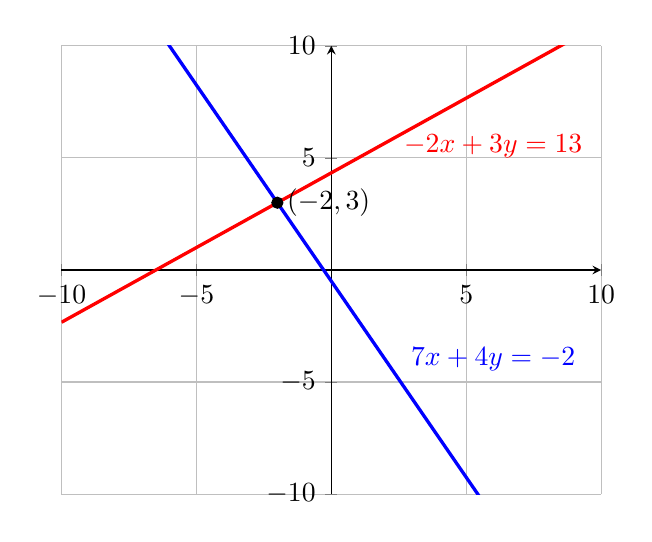
\begin{tikzpicture}
            \begin{axis}[
                axis lines=middle,
                grid=both,
                grid,
                ymin=-10,
                ymax=10,
                xmin=-10, 
                xmax=10
                ]       
                \addplot[mark=none, blue, very thick] coordinates {(-10,17) (10,-18)} node[above] at (axis cs:6,-5) {$7x+4y=-2$};
                \addplot[mark=none, red, very thick] coordinates {(-10,-2.3333) (10,11)} node[below] at (axis cs:6,6.5) {$-2x+3y=13$};
                \addplot[mark=*] coordinates {(-2,3)} node[right] at (axis cs:-2,3) {$(-2,3)$};
            \end{axis}
        \end{tikzpicture}
    \end{center}

    这种可视化方法也适用于三个方程和三个未知数的方程组,但这需要在三维空间中绘制图线。这在实践中可能很难做到,但在技术上是可行的。同样的概念也适用于多个方程和多个未知数,但在四维或更高维上画``线''对我们人类来说是可能是无法想象的!
\end{method}

\begin{method}{多于两个变量:消元!}
    该方法的下一部分建立在第一部分的基础上,通过不断应用第一部分的方法,将两个以上方程(和未知数)的方程组简化为更小的方程组,最终得到两个方程和两个未知数的方程组。我们通过一个三个方程和三个未知数的方程组来说明该方法,如下所示:
    $$
    \begin{cases}
        \enspace\: 6x - 3y + \enspace z = -1 \\
        -3x + 4y - 2z = 12 \\
        \enspace\: 5x + \enspace y + 8z = 6
    \end{cases}
    $$
    第一个目标是消除三个变量中的一个。本质上,这可以通过两种方式之一来完成,就像两个方程和两个未知数的方法一样。假设我们要从方程组中消除 $z$;我们可以尝试以某种方式用 $x$ 和 $y$ 来表示 $z$ 并代入,或者我们可以将某些方程乘以系数并相加,从而消除 $z$。这里唯一的区别是,无论我们选择哪种方法,我们都需要执行两次。我们用第一个方程得到
    \[z = -6x + 3y - 1\]
    将 $z$ 的表达式代入第二个和第三个方程后,我们将得到一个由两个方程和两个未知数组成的方程组。

    思考这个问题的一种方法是,我们需要来自所有三个方程的信息才能最终得出答案,因此在将方程组简化为两个方程时,我们需要以某种方式保留来自所有三个原始方程的信息。$z$ 的表达式来自第一个方程,因此我们需要将其代入其他两个方程以保留我们需要的所有信息。

    将其与以下步骤序列进行比较:整理第一个方程以分离 $z$ 并将其代入第二个方程,然后整理第二个方程式以分离 $z$,将其代入第一个方程。会发生什么?直觉告诉我们,在某种程度上``丢失''了第三个方程的信息,没错,我们将获得一个由两个方程和两个未知数组成的方程组,但它没有足够的信息得到 $x$ 和 $y$ 的唯一解。如果你真的执行了我们刚才描述的步骤(试着这样做来检查我们的工作),化简到最简后,可以得到以下两个方程的``方程组'':
    $$
    \begin{cases}
        9x - 2y = 10 \\
        \frac{9}{2}x - \:y = 5
    \end{cases}
    $$
    这两个方程其实是同一个方程!因此,我们实际上无法求解 $x$ 和 $y$ 的唯一值。

    让我们回到原来的位置,将上面 $z$ 的表达式代入第二和第三个方程
    \begin{align*}
        -3x + 4y - 2 \cdot (-6x + 3y - 1) &= 12 \\
        5x + y + 8 \cdot (-6x + 3y - 1) &= 6
    \end{align*}
    然后化简
    \begin{align*}
        9x - 2y &= 10 \\
        -43x + 25y &= 14
    \end{align*}
    应用第一个问题中的方法之一将解出 $(x, y) = (2, 4)$。有了这两个值,我们就可以代入三个原始方程中的任意一个并求出 $z$;更好的做法是,我们可以使用从第一个方程中得到的 $z$ 的表达式:
    \[z = -6x + 3y - 1 = -6 \cdot (2) + 3 \cdot 4 = 1 = -12 + 12 - 1 = -1\]
\end{method}

\begin{method}{多于两个变量:另一种消元方法!}
    将方程组从三个方程简化为两个方程的另一种方法与前面的``乘加''法有关。使用上面具有三个方程的方程组,我们可能会注意到,第一个方程乘以 $8$,第二个方程乘以 $4$ 后,所有三个方程中 $z$ 的系数都是 $\pm 8$。这使我们能够以简便的方式对方程进行加/减,将方程组简化为两个方程和两个未知数。具体来说,让我们做一遍刚才提到的操作
    \begin{align*}
        48x - 24y + 8z &= -8 \\
        -12x + 16y - 8z &= 48 \\
        5x + y + 8z &= 6
    \end{align*}
    然后将第一个方程与第二个方程相加
    \begin{align*}
        (48x - 12x) + (-24y + 16y) + (8z - 8z) &= -8 + 48 \\
        36x - 8y &= 40
    \end{align*}
    接着将第二个方程与第三个方程相加
    \begin{align*}
        (-12x + 5x) + (16y + y) + (-8z + 8z) &= 48 + 6 \\
        -7x + 17y &= 54
    \end{align*}
    上面操作将产生了两个仅包含 $x$和 $y$ 的方程;此外,我们结合了所有三个原始方程的信息来生成这些方程,所以我们可以确信我们没有``丢失''任何东西。用我们之前讨论的任意一种方法解此新方程组
    $$
    \begin{cases}
        \: 36x - \enspace 8y = 40 \\
        -7x + 17y = 54  
    \end{cases}
    $$
    都会解得 $(x, y) = (2, 4)$。将 $x$ 和 $y$ 的值代入三个原始方程中的任意一个并求出 $z$,即可得到我们要求的最终答案。

    我们也可以执行类似的步骤,从方程组中消除 $y$;例如,我们可以将第一个方程乘以 $4$ 与第二个方程乘以 $3$ 相加,然后用第二个方程减去第三个方程乘以 $4$。这些方法中的任何一种都会得到相同的最终答案,只是其中一些可能会缩短算术步骤或带来``更好计算''的数字(即更少的分数,更小的乘法,等等)。求解具有更多方程的方程组的一般过程:将方程相乘并相加,从方程组中消除一个变量,然后继续这样做,直到只有两个方程和两个未知数;然后,求解这两个变量的值,并反向代入运算,用这些值来求解已消除变量的值。
\end{method}

\subsubsection*{代数练习}

\begin{problem}
    求解关于 $(x, y, z)$ 的以下方程组:

    $$
    \begin{cases}
        \enspace x+y+z=15\\
        2x-y+z=8\\
        x-2y-z=-2
    \end{cases}
    $$

    求解关于 $(x, y, z)$ 的类似方程组:

    $$
    \begin{cases}
        \enspace x+y+z=15\\
        2x-y+z=9\\
        x-2y-z=-2
    \end{cases}
    $$

    比较两个方程组之间 $x$、$y$ 和 $z$ 值的变化。

    哪个变量变化最大?哪个最少?这些变化的比例是多少?

    通过改变方程组第二个方程右侧的常数,你可以使这个比率变多大/多小?
\end{problem}

\begin{problem}
    父亲、母亲和儿子坐在餐厅里吃饭,这时另一个由父亲、母亲和儿子组成的家庭走过来。第二个家庭惊讶于他们与第一个家庭如此相似,于是就问第一个家庭:``你们三个多大了?我猜我们的年龄都差不多''。第一个家庭的父亲恰好是一位数学家,不愿意轻易泄露家人的年龄,于是用一种巧妙的方式``透露''给其他人。他说:``我们现在的年龄加起来是 $72$ 岁,而我恰好是我儿子的六倍。然而,将来当我只是他年龄的两倍时,我们的年龄加起来将是我们现在年龄加起来的两倍。你猜我们多少岁?''\\
    三个家庭成员的年龄有多大?
\end{problem}

% !TeX root = ../../../book.tex
\subsection{多项式}

有时我们会遇到变量的平方、立方或更高次幂。一般来说,多项式是一种函数,它包含一个或多个变量的整数次幂项,这些项乘以系数后相加。以下是一些多项式的例子:
\[x^2 - 7x + 1,\qquad 7p^6 + 5p^4 + 3p^2 + 2p,\qquad \frac{1}{2}z^2 + 9y^2z - 2y + z^3y^2 - 7z\]

这类函数在数学中非常常见,部分原因在于它们具有便利的性质,另一部分原因是它们在自然界中普遍存在。我们将在本书中频繁遇到它们。不过,现在让我们聚焦于只有一个\emph{输入变量}的多项式。

\subsubsection*{多项式的根}

有时,我们会在题目中定义一个多项式函数,并想知道是否存在某些输入值能使其输出为 $0$。使输出为 $0$ 的输入值称为多项式的\textbf{根}。

识别多项式根的一种方法是将其\textbf{因式分解}为线性项;也就是说,我们将函数表示为一系列乘法而非加法,因为这样我们就可以指出(至少)其中一个因子为 $0$ 时,输出才为 $0$。该技术背后的原理依赖于以下事实:

\begin{quote}
    \textbf{事实:}若 $a$ 和 $b$ 为实数且 $ab=0$,则 $a=0$ 或 $b=0$(或者两者都等于零)。
\end{quote}

\begin{example}
    我们来看一个具体的例子。尝试分解以下多项式:
    \[p(x) = x^2 + 6x + 8\]
    (将多项式定义为 $p(x)$ 是常见的做法,其中 $p$ 代表多项式,$x$ 是输入变量,$p(x)$ 是与输入值 $x$ 对应的输出值。)

    你可能已经注意到:
    \[p(x) = x^2 + 6x + 8 = (x + 4) \cdot (x + 2) = (x + 4)(x + 2)\]
    (当因子由括号分隔时,省略 $\cdot$ 符号是常见的做法,因此我们将采用这一约定。)

    此处因式分解成立,是因为我们逆向应用了分配律。逐步展开上述因式分解的过程如下:
    \begin{align*}
        p(x) &= (x + 4)(x + 2) \\
        &= x(x + 2) + 4(x + 2) \\
        &= (x^2 + 2x) + (4x + 8) \\
        &= x^2 + 2x + 4x + 8 = x^2 + 6x + 8
    \end{align*}

    通过因式分解,我们发现 $+4$ 和 $+2$ 的乘积为 $+8$,这正是常数项,而它们之和为 $+6$,这正是 $x$ 项的系数。了解展开过程后,我们可以直接写出因式分解而无需逐步验证。
\end{example}

\subsubsection*{二次因式分解}

让我们以上面示例为例,尝试推广到一般二次函数。若需分解二次多项式
\[p(x) = x^2 + bx + c\]
我们需要求解 $r$ 和 $s$ 的值,使得 $r \cdot s = c$ 且 $r + s = b$。通常可``通过试算''或直接观察方程快速得到合适的值(这正是前例采用的方法)。

若 $x^2$ 项的系数不是 $1$ 而是 $a$,该如何处理?注意到若对多项式 $\frac{p(x)}{a} = x^2 + \frac{b}{a}x + \frac{c}{a}$ 进行因式分解,则可以通过乘以 $a$ 得到原始多项式 $p(x)$ 的分解式。由于 $a \ne 0$(否则非二次多项式,无需分解),这不影响求根的目标。得到因式分解后,$p(x)$ 的根就很容易确定;由 $p(x) = 0$ 及上述事实可得
\begin{align*}
    0 = p(x) = (x + r)(x + s) & \quad \text{意味着\ } x + r = 0 \text{\ 或\ } x + s = 0 \\
    & \quad \text{ 即\ } x = -r \text{\ 或\ } x = -s
\end{align*}
也就是说,根为 $-r$ 和 $-s$。

对于 $p(x) = x^2 - a^2$ 形式的多项式(称为\textbf{平方差}),有快速分解技巧。根据前述方法,需求解 $r,s$ 满足 $rs = -a^2$ 且 $r + s = 0$(因 $p(x)$ 无 $x$ 项)。由第二个条件可得 $r = -s$,代入第一个条件得 $r^2 = a^2$。因此,令 $r = a$ 和 $s = -a$ 实现因式分解 $p(x) = (x - a)(x + a)$,故根为 $\pm a$(请注意,实际上 $r = -a$ 和 $s = a$ 也满足上述两个条件,但会得到 $p(x)$ 的相同的因式分解)。

类似技巧可以推广至更高\textbf{次}多项式(``次''指变量的最高幂次)。例如,对四次多项式
\[p(x) = 4x^4 - x^2 - 3\]
如果令 $y = x^2$ 并将其化为二次多项式,便可以轻松分解它
\[p(y) = 4y^2 - y - 3 = (4y + 3)(y - 1)\]
请注意,此处可直接基于 $y^2$, $y$ 的系数和常数项应用前述分解方法。这里,我们想要分解 $\frac{p(y)}{4} = y^2-\frac{1}{4}=\frac{3}{4}$,因此令 $rs = -\frac{3}{4}$ 且 $r + s =-\frac{1}{4}$;取 $r=-1, s=+\frac{3}{4}$ 满足条件,所以我们得到因式分解
\[\frac{p(x)}{4} = (y+(-1))\Big(y+\frac{3}{4}\Big)\]
化简得
\[p(x) = 4(y-1)\Big(y+\frac{3}{4}\Big) = (y-1)(4y+3)\]
这正是我们之前的方法。

\subsubsection*{一根一因子}

当然,这种识别根的技巧也可以逆向应用:如果我们能轻松找到多项式的根,就有助于识别其因子。例如,观察以下三次多项式,尝试``通过试算''找出根;也就是说,寻找使 $p(x)$ 为零的 $x$ 值:
\[p(x) = x^3 - 3x + 2\]
若尚未找到,不妨尝试代入一些``简单值'',如前几个正整数和负整数。此时可得 $p(1) = 1 - 3 + 2 = 0$。因此可知多项式 $p$ 的因式分解必含因子 $(x - 1)$,因为其对应根 $x = 1$。据此,将 $p(x)$ 除以因子 $(x - 1)$,即可进一步对商式因式分解,从而确定 $p$ 的所有根。

\subsubsection*{多项式``除法''}

我们如何对多项式进行除法运算呢?目标是找到另一个多项式 $q(x)$,使得 $p(x) = q(x) \cdot (x - 1)$,即计算 $\frac{p(x)}{x-1}$。一种方法是运用中学整数除法中的\textbf{长除法}原理,这一方法同样适用于多项式!回顾除法的工作原理,并尝试通过一些基本示例---例如 $22 \div 7$---来唤醒记忆。

现在,我们尝试将同样的原理应用于多项式。下面是将长除法的思想应用于 $\frac{x^3-3x+2}{x-1}$ 的示例:

\[
\arraycolsep=1pt
\begin{array}{*1r @{\hskip\arraycolsep}c@{\hskip\arraycolsep} *{9}r}
        &          &   &      &   & x^2 & + &  x & - & 2 &  \\
\cline{2-11}
x-1     & \longdiv &   & x^3  &   &  & -    & 3x & + & 2 &  \\
        &          & - & x^3  & + & x^2 &   &    &   &   &  \\
\cline{3-6}
        &          &   &      &   & x^2 & - & 3x &   &   &  \\
        &          &   &      & - & x^2 & + &  x &   &   &  \\
\cline{5-8}
        &          &   &      &   &     & - & 2x & + & 2 &  \\
        &          &   &      &   &     &   & 2x & - & 2 &  \\
\cline{7-11}
        &          &   &      &   &     &   &    &   & 0 &  \\
\end{array}
\]

每一步中,我们寻找能``消去''当前最高次项的最大``因子''。具体而言,由于被除式的首项为 $x^3$,除式的首项为 $x$,我们在商的位置写上 $x^2$。接着,将 $(x-1)$ 乘以 $x^2$,将结果置于被除式下方,相减后得到余数。

重复上述过程,直至商中出现常数项(即 $x^0$ 的倍数)并检查余数。本例余数为 $0$,表明我们得到了一个没有余数的因式分解。进一步分解所得二次多项式:注意到 $r=2, s=-1$ 满足 $r+s=1$ 且 $rs=-2$,因此结果二次多项式可以进一步分解,最终得到
\[p(x) = (x - 1)(x - 1)(x + 2) = (x - 1)^2(x + 2)\]

该多项式次数为 $3$,但仅有 $2$ 个根。这是否令人困惑?你能构造一个仅含 $1$ 个根的三次多项式吗?是否存在无实根的三次多项式?若要求四次多项式有 $4$ 个、$5$ 个或更多根,是否可能?为什么?推广到 $n$ 次多项式,根的数量与次数有何关系?

\subsubsection*{因式展开}

在解决某些问题时,我们可能需要将多项式从因式分解形式完全展开,以便确定特定项的系数。如何快速而准确地完成多项式乘法?本质上,这需要反复应用分配律。虽然逐步执行基本操作总能保证结果正确(当不确定答案时,建议返回仔细检查每一步),但我们可以省略中间步骤以提高效率。

当需要展开形如 $(a+b)^n$(其中 $a$ 和 $b$ 为任意常量或变量,$n$ 为整数)的因式时,存在一种特殊方法能显著减少计算量。这种方法利用\textbf{帕斯卡三角}来快速确定展开式中各项的系数。

帕斯卡三角是一种按三角形排列整数的结构,每行对应展开式中的某个 $n$ 值。其构造规则如下:前两行全为 $1$,三角形外侧``边''也全为 $1$;内部任意位置的数值等于其左上方与右上方两个数值之和。尝试自行生成前几行,并与下方三角进行对比以验证正确性。

\begin{center}
    \begin{tabular}{rccccccccc}
        $n=0$: &    &    &    &    &  1\\\noalign{\smallskip\smallskip}
        $n=1$: &    &    &    &  1 &    &  1\\\noalign{\smallskip\smallskip}
        $n=2$: &    &    &  1 &    &  2 &    &  1\\\noalign{\smallskip\smallskip}
        $n=3$: &    &  1 &    &  3 &    &  3 &    &  1\\\noalign{\smallskip\smallskip}
        $n=4$: &  1 &    &  4 &    &  6 &    &  4 &    &  1\\\noalign{\smallskip\smallskip}
    \end{tabular}
\end{center}

左侧标注的 $n$ 值对应展开式 $(a+b)^n$。展开式的每一项均为帕斯卡三角中的某个系数乘以 $a^kb^{n-k}$,其中 $k$ 的取值范围是 $0$ 到 $n$。这意味着每一项中 $a$ 与 $b$ 的指数之和恒为 $n$。三角形每一行的数字按 $a$ 的降幂顺序排列:首项系数对应 $a^n$,随后依次对应 $a^{n-1}b$,依此类推。

例如,展开 $(a + b)^2$ 时,读取 $n=2$ 行得到系数 $1, 2, 1$,分别对应 $a^2$, $ab$, $b^2$。因此:
\[(a + b)^2 = a^2 + 2ab + b^2\]
此例也可以轻松地手动完成展开。但对于 $(x^2+2)^4$ 这类问题,手动展开效率较低。使用帕斯卡三角可极大提高效率:$n = 4$ 行告诉我们 $a^4, a^3b, a^2b^2, ab^3, b^4$ 的系数分别为 $1, 4, 6, 4, 1$,其中 $a = x^2, b = 2$。因此,可得
\begin{align*}
    (x^2+2)^4 &=  1 \cdot (x^2)^4 + 4 \cdot (x^2)^3 \cdot 2 + 6 \cdot (x^2)^2 \cdot (2)^2 + 4 \cdot x^2 \cdot (2)^3 + 1 \cdot (2)^4 \\
    &=  x^8 + 4 \cdot x^6 \cdot 2 + 6 \cdot x^4 \cdot 4 + 4 \cdot x^2 \cdot 8 + 16 \\
    &= x^8 + 8x^6 + 24x^4 + 32x^2 + 16
\end{align*}
尝试逐步展开并进行比较。帕斯卡三角本身蕴含深刻的数学性质,尤其在\textbf{组合数学}中具有重要应用。后续我们将深入探讨其特性!例如,``将上方相邻两数相加''的构造规则为何能生成二项式系数?其严谨证明将在讨论\textbf{二项式定理}时给出(详见 \ref{sec:section8.4.4} 节)。

\subsubsection*{配方}

在探讨重要结果之前,我们还需要介绍一个与多项式相关的技巧。有时,将多项式重写为平方项与常数项之和是非常有用的,这样可以方便地分离变量和常量。这相当于添加再减去同一个特定项,因此,总的来说,向多项式中添加了 $0$,但通过精心选择该项,我们可以简洁地重写多项式。这个过程被称为\textbf{配方},即添加一项以构造平方因子,同时减去相应项来保持多项式等价。

让我们通过一个例子说明该过程,然后再尝试进行推广。考虑以下多项式:
\[p(x) = x^2 + 8x + 9\]
直接因式分解并不容易,因此尝试配方。我们希望得到形如 $(x + a)^2$ 的项,其中 $x$ 的系数为 $1$,因为多项式中 $x^2$ 项系数为 $1$。展开 $(x + a)^2$ 得 $x^2 + 2ax + a^2$。由于我们需要得到 $8x$,所以应该令 $a = 4$,展开后得到 $x^2 + 8x + 16$。但原多项式的常数项为 $9$,所以要向原多项式中加上 $7$ 再减去 $7$:
\[p(x) = x^2 + 8x + 9 + 7 - 7 = (x^2 + 8x + 16) - 7 = (x + 4)^2 - 7\]
上面的式子看起来眼熟吗?实际上,它是平方差结构,可进一步因式分解:
\begin{align*}
    p(x) &= x^2 + 8x + 9 = (x + 4)^2 - 7 = (x + 4)^2 - \Big(\sqrt 7\Big)^2 \\
    &= \Big(x+4+\sqrt 7\Big)\Big(x+4-\sqrt 7\Big)
\end{align*}
因此,该多项式的根为 $x=-4-\sqrt 7$ 和 $x=-4+\sqrt 7$。

现在推广到一般形式!设二次多项式为:
\[p(x) = ax^2 + bx + c\]
为了能够配方,需添加上并减去特定项。我们之前是如何找到该项的?考虑 $(rx + s)^2$ 展开后得 $r^2x^2 + 2rsx + s^2$,为匹配系数,令 $r^2 = a$,所以 $r = \sqrt{a}$。(注意,这里要求 $a \ge 0$!如果 $a<0$ 该如何处理?)再令 $2rs = b$,解得 $s = \frac{b}{2r} = \frac{b}{2\sqrt{a}}$,此时需添加 $s^2 = \frac{b^2}{4a}$,再从多项式中减去。

以下公式实现了上述步骤,并通过代数整理使表达式更``简洁'':
\begin{align*}
    p(x) &= ax^2 + bx + c = ax^2 + bx + \frac{b^2}{4a} + c - \frac{b^2}{4a}\\
    &=\Big(\sqrt{a}x+\frac{b}{2\sqrt{a}}\Big)^2+\Big(c- \frac{b^2}{4a}\Big)\\
    &=\Bigg(\sqrt{a}\Big(x+\frac{b}{2a}\Big)\Bigg)^2+\Big(c- \frac{b^2}{4a}\Big)\\
    &=a\Big(x+\frac{b}{2a}\Big)^2+\Big(c- \frac{b^2}{4a}\Big)
\end{align*}

至此,我们已掌握对任意二次多项式配方的方法!

\subsubsection*{可视化配方}

要记住上述配方过程,一个好方法是借助正方形和矩形面积的可视化表示。

假设 $a, b>0$,我们可以从几何角度将 $ax^2+bx$ 视为组合图形的面积。具体来说,我们将 $ax^2$ 项视为正方形的面积。这意味着正方形的边长为 $\sqrt{a} \cdot x$:

\begin{center}
    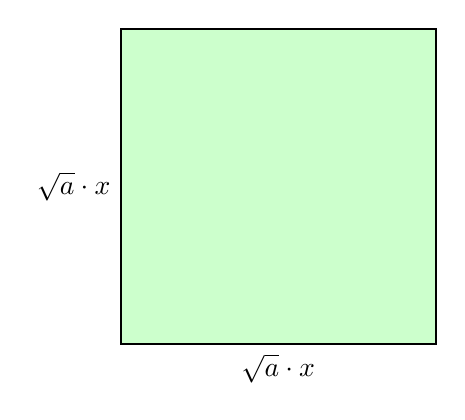
\begin{tikzpicture}[thick, scale=1]
        \fill [color=green,opacity=0.2] (0,0) rectangle +(4,4);
        \draw (0,0) rectangle +(4,4);
        \path (0,0) -- (4,0) node[midway,below] {$\sqrt{a}\cdot x$};
        \path (0,0) -- (0,4) node[midway,left] {$\sqrt{a}\cdot x$};
    \end{tikzpicture}
\end{center}

那么如何表示 $bx$ 项呢?配方本质是将原正方形扩展为更大的正方形。为此,我们在正方形周围添加矩形。将 $bx$ 代表的面积拆分为两个矩形,每个面积为 $\frac{b}{2}x$。由于矩形的一条边需与正方形边长一致(即 $\sqrt{a} \cdot x$),且面积为 $\frac{b}{2}x$,则另一条边长必为 $\frac{b}{2\sqrt{a}}$:

\begin{center}
    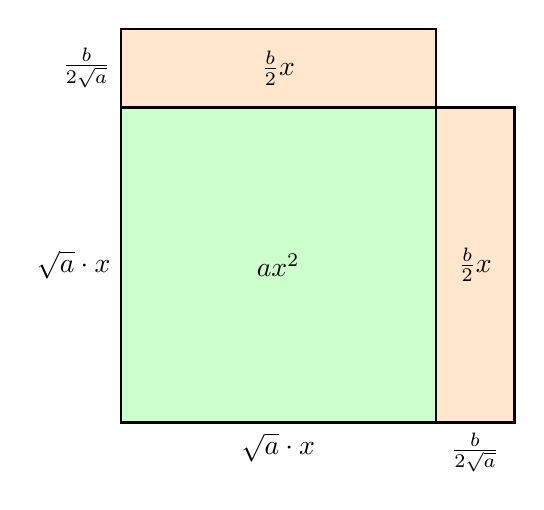
\begin{tikzpicture}[thick, scale=1]
        \fill [color=green,opacity=0.2] (0,0) rectangle +(4,4);
        \draw (0,0) rectangle +(4,4) node[pos=.5, align=center]{$ax^2$};
        \path (0,0) -- (4,0) node[midway,below] {$\sqrt{a}\cdot x$};
        \path (0,0) -- (0,4) node[midway,left] {$\sqrt{a}\cdot x$};

        \fill [color=orange,opacity=0.2] (4,0) rectangle +(1,4);
        \draw (4,0) rectangle +(1,4) node[pos=.5, align=center]{$\frac{b}{2}x$};
        \path (4,0) -- (5,0) node[midway,below] {$\frac{b}{2\sqrt{a}}$};

        \fill [color=orange,opacity=0.2] (0,4) rectangle +(4,1);
        \draw (0,4) rectangle +(4,1) node[pos=.5, align=center]{$\frac{b}{2}x$};
        \path (0,4) -- (0,5) node[midway,left] {$\frac{b}{2\sqrt{a}}$};
    \end{tikzpicture}
\end{center}

为使图形构成完整正方形,只需在右上角补上一个小正方形即可。小正方形边长为 $\frac{b}{2\sqrt{a}}$,故面积为 $\frac{b^2}{4a}$——这正是我们需要添加的项:

\begin{center}
    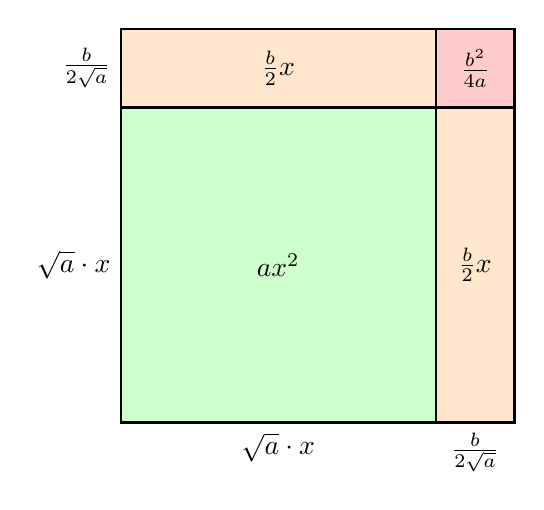
\begin{tikzpicture}[thick, scale=1]
        \fill [color=green,opacity=0.2] (0,0) rectangle +(4,4);
        \draw (0,0) rectangle +(4,4) node[pos=.5, align=center]{$ax^2$};
        \path (0,0) -- (4,0) node[midway,below] {$\sqrt{a}\cdot x$};
        \path (0,0) -- (0,4) node[midway,left] {$\sqrt{a}\cdot x$};

        \fill [color=orange,opacity=0.2] (4,0) rectangle +(1,4);
        \draw (4,0) rectangle +(1,4) node[pos=.5, align=center]{$\frac{b}{2}x$};
        \path (4,0) -- (5,0) node[midway,below] {$\frac{b}{2\sqrt{a}}$};

        \fill [color=orange,opacity=0.2] (0,4) rectangle +(4,1);
        \draw (0,4) rectangle +(4,1) node[pos=.5, align=center]{$\frac{b}{2}x$};
        \path (0,4) -- (0,5) node[midway,left] {$\frac{b}{2\sqrt{a}}$};

        \fill [color=red,opacity=0.2] (4,4) rectangle +(1,1);
        \draw (4,4) rectangle +(1,1) node[pos=.5, align=center]{$\frac{b^2}{4a}$};
    \end{tikzpicture}
\end{center}

看呐!这与代数推导的结果完全一致。添加此项后,表达式可分解为完全平方,只需再减去该项,以确保原表达式不变。

这是一个值得牢记的技巧,它能帮你理解配方的动机和步骤。但请思考:为何此方法成立?绘图时我们假设了 $a, b > 0$,那么当 $a$ 和 $b$ 为任意实数时,配方公式为何依然有效?

\subsubsection*{二次函数求根公式}

让我们回到多项式求根问题。具体来说,让我们回忆一下\textbf{二次函数求根公式}。你可能已经记住这个公式是``求解二次方程''的一种方法,但你知道它为什么成立吗?让我们试着弄清楚吧!一般来说,我们从以下形式的二次多项式开始
\[p(x) = ax^2 + bx + c\]
其中 $a \ne 0$(否则它就不是二次多项式),并且我们想要求 $p(x) = 0$ 时 $x$ 的值。(你是否尝试过回答我们上面提出的关于此类多项式有几个根的问题?在以下推导过程中请留意这一点。)将该多项式因式分解为线性因子很麻烦,所以我们使用上面介绍的方法:配方法。该方法的好处是,我们可以设 $p(x)=0$,并在配方后重新整理来求解 $x$。
\[0 = p(x) = ax^2 + bx + c =a\Big(x+\frac{b}{2a}\Big)^2+\Big(c- \frac{b^2}{4a}\Big)\]
化简可得
\[\frac{b^2}{4a} -c = a\Big(x+\frac{b}{2a}\Big)^2\]

现在,我们要开始``撤消''此处的配方来求解 $x$,这需要对两边求平方根。但如果 $\frac{b^2}{4a} -c < 0$ 呢?我们根本无法求平方根!如果 $\frac{b^2}{4a} -c = 0$ 呢?会有什么问题吗?当 $\frac{b^2}{4a} -c > 0$ 时会有什么问题吗?这些问题与多项式根的个数相关。你可能已经(正确地)推断出二次多项式最多可以有两个根,但在这里我们发现二次多项式可能有一个或零个根(及其原因)!

\begin{itemize}
    \item 当 $\frac{b^2}{4a} -c < 0$ 时,那么 $x$ 的任何值都\emph{不}可能满足上面推导中的最后一行公式。因此,$p(x)$ 无实数根。
    \item 当 $\frac{b^2}{4a} -c = 0$ 时,那么对上面最后一行公式两边取平方根是完全有效的,但只会产生\emph{唯一一个} $x$ 值:
    \begin{align*}
        \frac{b^2}{4a} -c = 0 &= a\Big(x+\frac{b}{2a}\Big)^2 \\
        0 &= x+\frac{b}{2a} \\
        x &= -\frac{b}{2a}
    \end{align*}
    \item 当 $\frac{b^2}{4a} -c > 0$ 时,此时 $p(x)$ 有\emph{两个}根,因为两边取平方根会引入两个可能的解。一般来说,当我们遇到像 $s^2 = t$ 这种情况时,可能的解是 $s =\sqrt{t}$ 和 $s = -\sqrt{t}$,但我们必须同时考虑两者(通常将其写做 $s = \pm\sqrt{t}$)。在这种情况下求解 $x$ 得
    \begin{align*}
        \frac{b^2}{4a} -c &= a\Big(x+\frac{b}{2a}\Big)^2 \\
        \pm\sqrt{\frac{b^2-4ac}{4a}} &= \sqrt{a}\Big(x+\frac{b}{2a}\Big) = \sqrt{a}x+\frac{b}{2\sqrt{a}} \\
        -\frac{b}{2\sqrt{a}}\pm\frac{\sqrt{b^2-4ac}}{\sqrt{4a}} &= \sqrt{a}x \\
        -\frac{b}{2a}\pm\frac{\sqrt{b^2-4ac}}{\sqrt{4a^2}} &= x
    \end{align*}
    现在,我们必须谨慎对待取平方根。一般来说,$\sqrt{4a^2} = \pm2a$,但分子上的平方根项已经有了一个 $\pm1$ 因子,分母上的因子不会改变这一点。因此,我们可以得出结论
    \[x = -\frac{b}{2a}\pm\frac{\sqrt{b^2-4ac}}{2a} = \frac{-b\pm\sqrt{b^2-4ac}}{2a}\]
    这就是二次函数求根公式!
\end{itemize}

请记住,推导的最后一种情况是在 $\frac{b^2}{4a} -c > 0$ 的假设下进行的。当 $\frac{b^2}{4a} -c = 0$ 时,该公式依然适用吗?在这种假设下,我们是否可以执行与上面相同的步骤?为什么可以或者为什么不行?

\subsubsection*{习题}

\begin{problem}
    求满足 $x-a$ 整除 $x^2+2ax-3$ 的 $a$ 的所有可能值。
\end{problem}
\begin{problem}
    求使得 $x^3 + b$ 可以被 $x + b$ 整除的 $b$ 的所有可能值。
\end{problem}
\begin{problem}
    对于任意自然数 $n$,将 $x^n - 1$ 因式分解。
\end{problem}
\begin{problem}
    求由如下公式定义的 $x$ 的值
    \[x = \sqrt{2+\sqrt{2+\sqrt{2+\sqrt{2+\dots}}}}\]
    \begin{hint}
        尝试用 $x$ 本身来表示无限嵌套根式。
    \end{hint}
\end{problem}
\begin{problem}
    用配方法证明:任意正数 $n$ 及其倒数之和始终大于或等于 $2$,并且唯一使和等于 $2$ 的数字是 $n = 1$。
    \begin{hint}
        求和,加减 $2$,然后重新整理。
    \end{hint}
\end{problem}
\begin{problem}
    如何求解形如 $ax^4 + bx^2 + c$ 的四次多项式的根?
\end{problem}


% !TeX root = ../../../book.tex
\subsection{集合漫谈}

我们已经提到了一些特定类型的数字,但我们想具体定义我们将来要使用的数字集。这些数字集合都由一个特定字母用黑板粗体表示。\textbf{自然数}(也称为整体数(whole numbers)或计数数(counting numbers))之所以被称为自然数,是因为当我们计数物体时,用自然数感觉很``自然''。自然数可以写做
\[\mathbb{N} = \{1, 2, 3, 4, 5, \dots\}\]
(自然数有一个更具体更技术性的定义,我们将在稍后解释。)\\
我们用 $\mathbb{N}$ 表示 ``自然(natural)''

使用 $\mathbb{N}$,我们可以定义一个相关的数字集合:所有\textbf{整数}的集合,它包含了自然数、$0$ 和负自然数。整数可以写做
\[\mathbb{Z} = \{\dots, -3, -2, -1, 0, 1, 2, 3, \dots\}\]
字母 $\mathbb{Z}$ 来自德语单词 \emph{Zahlen},意思是``数字''。

从整数集合,我们可以定义\textbf{有理数}的集合。这些数字可以表示为整数的比率,但它们似乎没有像集合 $\mathbb{N}$ 和 $\mathbb{Z}$ 那样自然的``列表'',所以我们不能像上面那样书写这个集合。为此,我们使用一个非常常见的集合表示法,如下所示:
\[\mathbb{Q} = \Big\{\frac{a}{b} \mid a,b \in \mathbb{Z} \text{ 且 } b \ne 0\Big\}\]
读作:
\begin{quote}
    ``有理数集是所有 $\frac{a}{b}$ 形式的数的集合,其中 $a$ 和 $b$ 都是整数,且 $b$ 不为零。''
\end{quote}
这表达了有理数是分数的必要信息,其中分子和分母都是整数(但分母不能为 $0$,因为除以 $0$ 是不允许的)。我们使用字母 $\mathbb{Q}$ 表示有理数,是因为 $\mathbb{R}$ 已经被用于表示实数,而 $\mathbb{Q}$ 是上一个可用的字母。此外,$\mathbb{Q}$ 包含所有整数的商,所以这也是有道理的!

\textbf{实数} $\mathbb{R}$ 有一个非常技术性的定义,遗憾的是,我们无法在本书中全面深入研究。(这恰恰表明,从数学上定义这个集合是多么困难!) 目前,思考实数的一种方法是通过\textbf{数轴}。实数是数轴上所有的数字,而 $\mathbb{N}$、$\mathbb{Z}$ 和 $\mathbb{Q}$ 中的数字是数轴上的特定数字,它们并不构成整条数轴。某种程度上,$\mathbb{R}$ 是 $\mathbb{Q}$ 的``补全'',即``填补有理数之间的空白''。


% !TeX root = ../../../book.tex
\subsection{符号加油站}\label{sec:section1.3.5}

一种流行且方便的求和与求积的写法是使用缩写符号,将多个项或因子写成一种通用的形式。例如,如果我们想谈论前 $500$ 个自然数之和,该怎么写呢?写出总和的全部 $500$ 项会很乏味,所以 $1+2+3+\dots+499+500$ 是更常见的写法。(事实上,我们已经使用过这样的省略号。 你明白我们的意思吗?)这种写法很流行,并且确实表达了观点,但一些数学家对中间多余的省略号感到不满。我们推迟到现在才讨论这个问题,是因为符号通常很难学习和理解。我们并没有立即用新符号轰炸你,而是诉诸我们对 ``$\dots$'' 作用的直观理解。

既然我们已经提出来了,让我们看看如何避免使用省略号。为了写出我们上面提到的求和,我们将使用以下符号:
\[1+2+3+\dots+499+500 = \sum_{i=1}^{500}i\]
大写西格玛 $\sum$ 来自对应英文字母 S 的希腊字母,代表``求和''。\textbf{索引} $i$ 告诉我们求和的各个项的值。在 $\sum$ 符号下面写 $i = 1$,在 $\sum$ 符号上面写 $500$ 意味着我们让 $i$ 表示 $1$ 到 $500$(含)之间的所有自然数值。我们将这些值代入求和项的通用表达式,在本例中就是 $i$。因此,根据要求,求和项为 $1,2,3,\dots,500$。通过改变求和项表达式和/或索引的值,试着找到一些其他的写法。如果我们想求前 $500$ 个偶自然数之和怎么办?想求 $500$ 以内(含)所有偶自然数又该怎么办呢?尝试用上面的符号样式写出这些求和。

与此相关的是 $\prod$ 表示法。如果我们想查看前 $500$ 个自然数的乘积,我们将遵循相同的约定来识别索引值和通项:
\[1+2+3+\dots+499+500 = \prod_{i=1}^{500}i\]
大写派 $\prod$ 来自对应英文字母 P 的希腊字母,代表``求积''。再次尝试通过更改求积项和/或索引值以不同的方式表达上面公式。如果我们想求前 $500$ 个偶自然数的乘积怎么办?想求 $500$ 以内(含)所有偶自然数之积又该怎么办呢?尝试用上面的符号样式写出这些求积。

\subsubsection*{问题}

\begin{problem}
    用自然语言来描述以下等式的含义:
    \[\sum_{i=1}^{n}i^2 = \frac{n(n+1)(2n+1)}{6}\]
\end{problem}
\begin{problem}
    用适当的符号表达 $2$ 的前 $n$ 次幂的和与积,从 $2^0=1$ 开始。你能证明这个求和和求积公式吗?
\end{problem}
\begin{problem}
    考虑 $17$ 到 $33$(含)之间的所有奇数之和。索引 $0$ 开始,用求和符号写出这个求和公式。现在试着将索引从 $1$ 开始,重写求和公式。现在试着将索引从 $8$ 开始,重写求和公式,然后将索引从 $9$ 开始。以下哪一个感觉``更自然''?为什么?
\end{problem}

\newpage
% !TeX root = ../../../book.tex
\section{智力谜题}\label{sec:section1.4}

让我们把迄今为止讨论过的一些原则付诸实践。具体来说,让我们研究一些有趣的数学难题并解释如何解决它们。这些问题都不涉及除基本代数和算术之外的知识,但这并不意味着它们``基础''或``简单'',因为解决并理解这些问题都涉及批判性思维技能和敏锐的洞察力。在此过程中,我们将运用我们已经提出的一些逻辑思想。我们可能需要用到多项式函数,或者用代数方法求解一些方程。我们可能需要仔细考虑论证的顺序和流程,确保一切都遵循前面的知识或推论。总的来说,我们还应该思考什么构成了我们发现事实的良好且有效的\emph{证明}!

% !TeX root = ../../../book.tex
\subsection{消失的钞票}

\subsubsection*{问题描述}

这个经典的谜题包含在一个关于分摊酒店房间费用的故事中:

\begin{quote}
    三个朋友自驾旅行,深夜入住酒店。值班店员说当晚只剩一间空房,三人合住需付 $30$ 美元。他们疲惫不堪,便同意合住,每人各付 $10$ 美元预付款。店员道谢后递过钥匙,三人随即去车上取行李。此时,前来换班的另一名店员发现前一名店员多收了房费:实际只需 $25$ 美元。于是他从收银机取出一张 $5$ 美元钞票,递给值班服务生说:``把钱退给 29 号房的客人,我们多收费了。''服务生点头后走向三人房间。客人开门时对退款又惊又喜。为公平起见,一人将钞票换成五张 $1$ 美元纸币,每人取回 $1$ 美元,剩余 $2$ 美元作为小费给了服务生。服务生道谢后离开。

    现在,三人每人实际支付 $9$ 美元房费,加上 $2$ 美元小费,总计 $29$ 美元。但他们最初支付了 $30$ 美元……消失的 $1$ 美元去哪儿了?!
\end{quote}

请仔细思考一下,然后再翻页阅读解答。

\clearpage

\subsubsection*{解答:追踪资金流向}

你搞明白了吗?其实没有任何东西凭空``消失''。这个谜题的目的就是迷惑读者,误导他们去寻找不存在的事物。题目中的数字经过精心设计,使``消失的金额''仅为 $1$ 美元,让读者误以为发生了什么神秘事件。但通过细致的逻辑分析,你会发现最终提问本身并不合理:它利用了读者对情境的误解,使其忽视逻辑推理。若数字差异变得更大,人们便不会执着于寻找``消失的钞票''。

首先,让我们分析一下在这个特殊案例中到底发生了什么。关键在于厘清资金的实际流向。我们可将参与者分为两组:朋友群体(记为 $F$)和酒店员工群体(包括店员与服务生,记为 $H$)。现在,让我们重现资金转移步骤:

\begin{enumerate}
    \item $F$ 支付 $H \quad 30$ 美元(原始房费)
    \item $H$ 退还 $F \quad \enspace 5$ 美元(多收房费退款)
    \item $F$ 支付 $H \quad \enspace 2$ 美元(服务生小费)
    \item 净变化:$F$ 向 $H$ 支付 $30 \text{\ 美元} -5 \text{\ 美元} + 2 \text{\ 美元} = 27 \text{\ 美元}$
\end{enumerate}

这样就清晰了:退款 $5$ 美元使实际房费变为 $25$ 美元,三人每人付了 $9$ 美元,再加上服务生的小费,共计 $27$ 美元。谜题错误地将小费与房费相加,但 $27$ 美元已包含全部支出。通过追踪群体间的资金流动,我们能准确还原交易过程。

\subsubsection*{泛化:改变数字}

让我们应用上述方法来修改问题,通过改变数字消除对``消失的钞票''的情感依赖,同时放大金额差异。首先定义变量表示各步骤的金额。与其``测试''特定数值,不如引入变量实现``一次性全面验证''。

设 $3n$ 表示三人首次支付的房费总额($n$ 为每人支付金额)。退款金额设为 $3r + 2$,其中 $r$ 为每人实际退款,$2$ 为给服务生的小费。下面用变量重述该问题:

\begin{quote}
    三个朋友自驾旅行,深夜入住酒店。值班店员说当晚只剩一间空房,三人合住需付 $3n$ 美元。他们疲惫不堪,便同意合住,每人各付 $n$ 美元预付款。店员道谢后递过钥匙,三人随即去车上取行李。此时,前来换班的另一名店员发现前一名店员多收了房费:实际只需 $3n - (3r + 2)$ 美元。于是他从收银机取出一张 $3r + 2$ 美元钞票,递给值班服务生说:``把钱退给 29 号房的客人,我们多收费了。''服务生点头后走向三人房间。客人开门时对退款又惊又喜。为公平起见,三人每人取回 $r$ 美元,剩余 $2$ 美元作为小费给了服务生。服务生道谢后离开。

    现在,三人每人实际支付 $n-r$ 美元房费,加上 $2$ 美元小费,总计 $3(n-r)+2$ 美元。但他们最初支付了 $3n$ 美元……消失的 $3n - [3(n - r) + 2]=3r - 2$ 美元去哪儿了?!
\end{quote}

现在问题是否更清晰了?正如我们之前解释的那样,差异源于原文将小费加入退款后的房费,再与初始 $3n$ 美元房费进行比较。正确的比较应该是,实际房费支出 $3(n-r) = 3n - 3r$,与退费后房费与小费之和 $[3n-(3r+2)] + 2 = 3n-3r$ 进行比较。两者完全相等!

\subsubsection*{泛化:留给你的问题}

谜题的原始陈述中,$n=10, r=1$,因此``消失的钞票''神奇地变为 $3r-2=1$。如果我们选择更大的数值——例如 $n=100, r=10$——那么 $300$ 美元的房间实际花费 $268$ 美元,服务生会退还三人 $32$ 美元,他们每人拿回 $10$ 美元,服务生保留 $2$ 美元,差额就变成了 $28$ 美元。真的会有人相信 $28$ 美元在此交易中凭空消失了吗?如果我们使用更大的 $n$ 和 $r$ 值呢?你能把差额扩大到多大?或缩小到多小?给定所需的差额(以美元为单位),你能找到满足条件的 $n$ 和 $r$ 的值吗?有多少种方法可以做到这一点?

\subsubsection*{解题心得}

逻辑和理性思维在解决难题时至关重要,因为情绪容易误导人。如果我们最初将这个谜题表述为``消失的 $28$ 美元'',你会有同样的反应吗?在试图回溯并弄清真相之前,你是否会感到短暂的困惑?


% !TeX root = ../../../book.tex
\subsection{高斯驾到}\label{sec:section1.4.2}

\subsubsection*{问题描述}

数学界流传着一个关于史上最伟大数学家兼物理学家之一——卡尔·弗里德里希·高斯 (Carl Friedrich Gauss) 的著名轶事。无论故事真实与否,其魅力令无数人深信不疑。高斯活跃于 18 世纪末至 19 世纪中叶,在数论、复分析、光学、几何学及天文学等诸多领域做出了奠基性贡献。请阅读下面这则故事,设想自己(无论童年或现在)会如何应对,然后再继续探讨。

\begin{quote}
    清晨,小学教室里喧闹的学生令老师不胜其烦。为获得片刻安宁,他急需让学生们专注做事。老师高声要求学生取出石板和粉笔。待众人准备就绪,他布置了一道题目:计算从 $1$ 到 $100$ 所有整数之和,并承诺最先完成者可担任当日助教。老师回到座位,料想繁重的计算将让学生们安静许久。不料仅过一分钟,一个男孩便带着写有答案的石板前来。老师惊讶之余亲自验算,结果证实男孩答案完全正确。他是如何快速完成计算的?
\end{quote}

请认真思考后再翻阅解答。请注意:这则故事``发生''在计算器尚未问世的年代,解题只能依靠纸笔与心算能力。

\clearpage

\subsubsection*{解答:简化计算}

也许你已经找到了窍门。实际上,这个问题有多种解法,它们大多基于相同的核心思路:尽量减少所需的计算量。

如果简单地遍历这 $100$ 个数字并逐个累加,需要进行 $99$ 次加法,且运算数字会越来越大。当然,技巧不仅仅在于更快地执行加法,而在于从根本上提高计算效率。我们知道,乘法本质上是数字与其自身的重复加法。因此,如果能找到合适的数字进行重复自加,就有可能将大量加法简化为一次乘法。

另一个关键点是加法满足\textbf{结合律}和\textbf{交换律},这意味着加法的顺序不影响最终结果。具体而言,无论将数字从 $1$ 加到 $100$ 还是从 $100$ 加到 $1$,其总和 $S$ 都相同。我们可以这样表示:
\begin{center}
    \begin{tabular}{ccccccccccccccc}
          1 & + &   2 & + &   3 & + & \dots & + &  98 & + &  99 & + & 100 & = & S\\\noalign{\smallskip\smallskip}
        100 & + &  99 & + &  97 & + & \dots & + &   3 & + &   2 & + &   1 & = & S\\\noalign{\smallskip\smallskip}
        \hline
        101 & + & 101 & + & 101 & + & \dots & + & 101 & + & 101 & + & 101 & = & 2S\\\noalign{\smallskip\smallskip}
    \end{tabular}
\end{center}
注意,我们以两种顺序写出了总和 $S$。将这两个等式逐项相加,得到总和 $2S$ 的表达式。这个新表达式可直接转换为乘法,因为有 $100$ 项,每项都等于 $101$。因此:
\begin{align*}
    2S &= 101 \cdot 100 \\
     S &= 101 \cdot 50 = 5050
\end{align*}
这比执行 $99$ 次加法要快得多。事实上,只要稍加练习,我们完全能在脑海中完成整个计算过程!

\subsubsection*{另一种解法:配对法}

解决该问题的相似思路是省去两行相加的中间步骤,直接将原始求和中的数字配对,如下所示:
\begin{align*}
    S &= 1 + 2 + 3 + \dots + 98 + 99 + 100 \\
    &= (1 + 100) + (2 + 99) + (3 + 98) + \dots + (49 + 52) + (50 + 51) \\
    &= 101 + 101 + \dots + 101 = 50 \cdot 101 = 5050
\end{align*}
该方法与前述解法本质相同,均利用加法交换律和结合律重组求和项,只是跳过了求 $2S$ 表达式然后再除以 $2$ 这一中间步骤。

\subsubsection*{泛化:$n$ 为偶数}

如果老师要求学生计算 $1$ 到 $1000$ 的数字之和呢?学生是否会抗议?高斯能否同样迅速作答?我们虽不确定前两个问题的答案,但相信你一定能轻松解决。这里唯一不同的是,我们需要创建 $500$ 组配对(而非 $50$ 组),每组之和为 $1001$(而非 $101$),因此结果为
\[1 + 2 + 3 + \dots + 998 + 999 + 1000 = 1001 \cdot 500 = 500500\]

看起来是不是存在某种规律呢?你觉得你能在不进行乘法的情况下立即说出 $1$ 到 $100$ 万之间所有数字之和是多少吗?

\subsubsection*{泛化:$n$ 为奇数}

如果老师要求的是前 $99$ 个数字之和呢?配对法是否仍然适用?让我们验证一下:
\begin{align*}
    S &= 1 + 2 + 3 + \dots + 97 + 98 + 99 \\
    &= (1 + 99) + (2 + 98) + (3 + 97) + \dots + (48 + 52) + (49 + 51) + 50 \\
    &= (49 \cdot 100) + 50 = 4950
\end{align*}
请注意,总项数为奇数,因此无法将所有数字完全配对,必须在乘法结果上加上中间项 $50$。是否有其他配对方式?
\begin{align*}
    S &= 1 + 2 + 3 + \dots + 97 + 98 + 99 \\
    &= (1 + 98) + (2 + 97) + (3 + 96) + \dots + (48 + 51) + (49 + 50) + 99 \\
    &= (49 \cdot 99) + 99 = 50 \cdot 99 = 4950
\end{align*}
这种方法\emph{看起来}与原始谜题的结果更相似,因为我们只执行\emph{一次}乘法。这是巧合吗?请尝试用相同方法计算其他奇数项之和:前 $7$ 个整数之和是多少?前 $29$ 个呢?前 $999$ 个呢?前 $999999$ 个呢?

\subsubsection*{泛化:任意 $n$}

让我们从个案研究中抽离出来,尝试从更一般的视角解决这个问题。假设老师向学生提出了以下问题:
\begin{quote}
    给出前 $n$ 个自然数之和的公式。我需要一个具体的公式,这样当有人告诉我 $n$ 的值时,我就能直接代入并快速得到答案。
\end{quote}

第二句的说明排除了其他方法。虽然我们之前提出过一些简单算法,但现在被要求给出一个直接计算的公式。该如何入手呢?根据之前的观察,分情况讨论 $n$ 的奇偶性是一个合理的策略。我们发现奇偶情况下的配对结果略有差异,因此先讨论其中一种情况,再讨论另一种。在每种情况下,我们都寻求 $S(n) = 1 + 2 + 3 + \dots + (n - 2) + (n - 1) + n$ 的表达式。这里用 $S(n)$ 表示这个和依赖于 $n$ 的值。

如果 $n$ 为偶数,我们可以将所有数完美配对:
\begin{align*}
    S(n) &= 1 + 2 + 3 + \dots + \Big(\frac{n}{2}-1\Big) + \frac{n}{2} + \Big(\frac{n}{2}+1\Big) + \dots + (n - 2) + (n - 1) + n\\
    &=  (1 + n) + \big(2 + (n - 1)\big) + \big(3 + (n - 2)\big) + \dots + \Big(\big(\frac{n}{2}-1\big)+\big(\frac{n}{2}+2\big)\Big) + \Big(\frac{n}{2}+\big(\frac{n}{2}+1\big)\Big) \\
    &= (n+1)\frac{n}{2} = \frac{n^2+n}{2}
\end{align*}

将已知结果的偶数(如 $n=100, 1000, 1000000$)代入公式进行验证。注意,公式中出现 $\frac{n}{2}$ 是合理的,因为 $n$ 为偶数,$\frac{n}{2}$ 必为整数。

如果 $n$ 为奇数呢?此时无法将所有数完全配对,需要巧妙处理。回想前 $99$ 项求和的方法,通过暂时忽略末项 $n$,将剩余项配对。有趣的是,每对之和恰好等于末项 $n$。让我们尝试运用此方法:
\begin{align*}
    S(n) &= 1 + 2 + 3 + \dots + \Big(\frac{n-1}{2}-1\Big) + \frac{n-1}{2} + \Big(\frac{n-1}{2}+1\Big) + \dots + (n - 2) + (n - 1) + n\\
    &=  \big(1 + (n-1)\big) + \big(2 + (n - 2)\big) + \dots + \Big(\big(\frac{n-1}{2}\big)+\big(\frac{n-1}{2}+1\big)\Big) + n \\
    &= n+n+ \dots + \Big(\frac{2n-2}{2}+1\Big) +n = (n+n+\dots+n)+n
\end{align*}

这表明每对数字之和为 $n$,即我们最初忽略的末项。现在计算配对数量:第一对是 $(1, n - 1)$,第二对是 $(2, n - 2)$,依此类推,最后一对的首项为 $\frac{n-1}{2}$。因此共有 $\frac{n-1}{2}$ 对。(注意 $n$ 为奇数保证了 $n-1$ 为偶数,故 $\frac{n-1}{2}$ 为整数。请回顾推导过程,确认每一步的有效性。)加上末项 $n$,总和可表示为:
\[S(n) = \Big(\frac{n-1}{2} + 1\Big) \cdot n = \Big(\frac{n-1}{2} + \frac{2}{2}\Big) \cdot n = \frac{n+1}{2} \cdot n = \frac{n^2+n}{2}\] 

令人惊讶的是,这与 $n$ 为偶数时得到的公式完全相同!你是否感到意外?虽然奇偶情况的解法相似,但并无明显迹象预示结果会一致。这对我们有什么启示?数学家面对这种``巧合''时,会思考是否存在\emph{更简洁}、\emph{更普适}的解法——能否用一种方法同时处理奇数和偶数\emph{两种}情况?既然结果相同,这样的方法很可能存在。请在继续阅读前先思考一下这个问题。

\subsubsection*{泛化:任意 $n$, \emph{不}分开讨论}

事实证明,我们在之前讨论这道谜题时已经暗示过另一种方法。还记得将正序求和写在一行、倒序求和写在另一行并将它们相加吗?当时处理奇偶性问题时,我们因看似步骤繁琐而避开了此法;``配对法''似乎更快捷,所以我们便采用了配对法。但若重新审视``两次相加''这一方法,会得到什么?我们会发现:
\begin{center}
    \begin{tabular}{ccccccccccc}
           1  & + &     2 & + & \dots & + & (n-1) & + &     n & = & S(n)\\\noalign{\smallskip\smallskip}
           n  & + & (n-1) & + & \dots & + &     2 & + &     1 & = & S(n)\\\noalign{\smallskip\smallskip}
        \hline
        (n+1) & + & (n+1) & + & \dots & + & (n+1) & + & (n+1) & = & 2S(n)\\\noalign{\smallskip\smallskip}
    \end{tabular}
\end{center}
此时第三行求和包含 $n$ 项,每项均为 $(n + 1)$。因此:
\begin{align*}
    2S &= (n+1) \cdot n \\
     S &= \frac{1}{2}(n+1) \cdot n = \frac{n^2+n}{2}
\end{align*}
这正是此前推导的公式,而此处的推导过程完全不依赖 $n$ 的奇偶性!(请回顾上述步骤并自行验证 $n$ 的奇偶性确实无关紧要。)

\subsubsection*{第三种解法:可视化图表}

在结束此问题之前,我们介绍一种几何解法。我们将求和 $S(n)$ 与正方形的面积关联,并将求和的各项($1, 2, 3, \dots, n - 1, n$)可视化为正方形的一部分。具体来说,考虑一个 $n \times n$ 的正方形,并将各项表示为宽度为一个单位、高度递增的矩形。见下图:

\begin{center}
    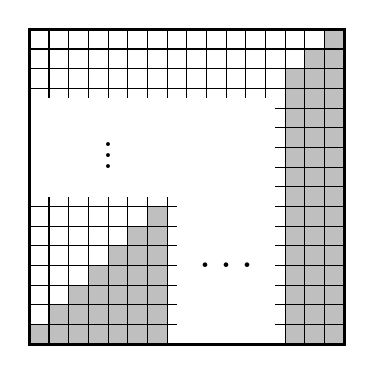
\begin{tikzpicture}[scale=0.5, x=0.5cm, y=0.5cm, font=\LARGE]
        \foreach \x in {0,...,15} 
            \foreach \y in {0,...,15}
                {
                    \pgfmathparse{(\x >= \y && (\x<7 || \x>12)) ? "lightgray" : "white"}
                    \edef\colour{\pgfmathresult}
                    \path[fill=\colour] (\x,\y) rectangle ++ (1,1);
                    \draw[black] (\x,\y) rectangle ++ (1,1);
                }
        \fill[white] (0, 7.5) rectangle ++ (8,5) node[color=black, pos=.5, align=center]{$\vdots$};
        \fill[white] (7.5, 0) rectangle ++ (5,8) node[color=black, pos=.5, align=center]{$\dots$};
        \fill[white] (7.5, 7.5) rectangle ++ (5,5) node[color=black, pos=.5, align=center]{$\iddots$};
        \draw[very thick, black] (0, 0) rectangle ++ (16,16);
    \end{tikzpicture}
\end{center}

现在,要求 $S(n)$ 的公式等价于计算正方形内所有矩形覆盖的\emph{面积}。直接相加各矩形面积只是重复原问题,因此我们需要将该面积与正方形的总面积关联。为此,考虑剩余区域,如何描述未被矩形覆盖的部分?观察第一个 $1 \times 1$ 矩形正上方的区域:它是一个尺寸为 $(n - 1) \times 1$ 的矩形。

类似地,$2 \times 1$ 矩形上方的区域是一个 $(n-2) \times 1$ 矩形。此模式持续下去!最终,在 $(n - 1) \times 1$ 矩形上方为一个 $1 \times 1$ 矩形,而最后一个 $n \times 1$ 矩形上方无区域。这些矩形的总面积类似于 $S(n)$,但缺少最后一项 $n$。现在,将所有矩形的面积与 $S(n)$ 和正方形面积关联:
\[n^2 = S(n) + (S(n) - n) = 2S(n) - n\]
解得
\[S(n) = \frac{n^2+n}{2}\]
与我们之前得到的公式一致!

\subsubsection*{解题心得}

有时,问题有多种解法。有些方法易于构思但难于求解;有些难以想到但求解简洁;还有些可能根本无效!通常无法预判哪种方法有效,因此建议动手尝试并观察结果。记录尝试的过程和结果,以便后续重新评估。这是数学学习中需牢记的原则:我们并非总能立即知晓正确路径,偶尔会陷入困境或走入死胡同。这不应令人沮丧;它是学习的一部分。

作为练习,尝试为 $n$ 为奇数的情况重新``配对'',不忽略求和的最后一项,而是分离中间项并将数字从外向内配对。这会得到相同结果吗?该方法是否比原解法更简便、更快速或有所不同呢?或者,对于 $n$ 为偶数的情况,令 $n=2k$ 会怎样?对于 $n$ 为奇数又该如何操作?这种表示会改变处理过程吗?会使问题更容易处理吗?现在,你能构思一种全新的解法吗?


% !TeX root = ../../../book.tex
\subsection{求和杂谈}\label{sec:section1.4.3}

\subsubsection*{奇数求和:观察模式}

既然谈到了整数求和,不妨探讨一些相关问题。首先介绍一种有趣的几何方法来解释奇数之和:将 $1$ 表示为 $1 \times 1$ 方块,随后每个连续的更大奇数可视作由 $1 \times 1$ 方块构成的直角,它能完美贴合前一个图形。我们为什么要这样做?因为奇数序列中连续项相差 $2$,每次将直角边增加 $1$ 个方块,即可与原图形无缝衔接,逐步构建更大的正方形!

\begin{center}
    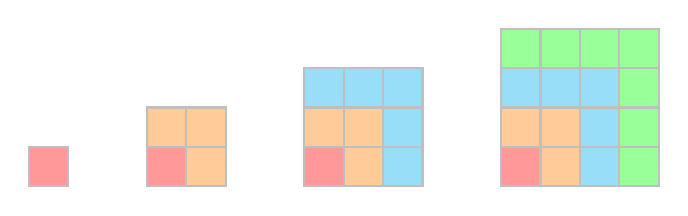
\begin{tikzpicture}[thick,scale=0.5, x=1cm, y=1cm]
        \foreach \x in {0,3,7,12}
        {
            \fill[red!40!white] (\x, 0) rectangle ++ (1,1);
            \draw[lightgray] (\x, 0) rectangle ++ (1,1);
        }

        \foreach \x in {3,7,12}
        {
            \foreach \i in {0,1}
            {
                \fill[orange!40!white] (\x+\i, 1) rectangle ++ (1,1);
                \draw[lightgray] (\x+\i, 1) rectangle ++ (1,1);
                \fill[orange!40!white] (\x+1, \i) rectangle ++ (1,1);
                \draw[lightgray] (\x+1, \i) rectangle ++ (1,1);
            }
        }

        \foreach \x in {7,12}
        {
            \foreach \i in {0,...,2}
            {
                \fill[cyan!40!white] (\x+\i, 2) rectangle ++ (1,1);
                \draw[lightgray] (\x+\i, 2) rectangle ++ (1,1);
                \fill[cyan!40!white] (\x+2, \i) rectangle ++ (1,1);
                \draw[lightgray] (\x+2, \i) rectangle ++ (1,1);
            }
        }

        \foreach \i in {0,...,3}
        {
            \fill[green!40!white] (12+\i, 3) rectangle ++ (1,1);
            \draw[lightgray] (12+\i, 3) rectangle ++ (1,1);
            \fill[green!40!white] (12+3, \i) rectangle ++ (1,1);
            \draw[lightgray] (12+3, \i) rectangle ++ (1,1);
        }
    \end{tikzpicture}
\end{center}

这种模式会持续下去吗?若确信如此,要如何严格证明?几何图案隐含的数值之和有何意义?这是首先要回答的问题,因为尽管几何呈现直观优美,但却难以精确操作和验证,最终无法给出严谨的\emph{证明}。本质上,仅展示前几项并宣称``看,它成立!''并不构成数学证明,因此需要寻求更优的表述方式。这并非否定图形的意义与美感,其运作机制确实提供了有价值的数学洞察,但归根结底,这便是其所能带给我们的上限。

\subsubsection*{奇数求和:证明我们的发现}

让我们尝试用数字形式写出上图所表示的求和。每个正方形由 $1 \times 1$ 块组成,每个比前一个多两块,因此每个正方形对应一个求和,例如
\[1 \qquad 1+3 \qquad 1+3+5 \qquad 1+3+5+7 \]
依此类推。从这些求和中,我们注意到它们都是平方数:
\[1=1^2 \qquad 1+3=4=2^2 \qquad 1+3+5=9=3^2 \qquad 1+3+5+7=16=4^2 \]
\emph{这}正是我们想要证明的模式;它对应于之前观察到的几何图形,但现在是我们可以操作的数学形式。现在,让我们思考如何证明这一点。这种模式与我们之前见过的模式相似吗?我们之前已经证明过关于整数之和的结果了吗?当然!回顾之前的题目,事实上在某些方面,我们已经证明了
\[1 + 2 + 3 + \dots + (n_1) + n =\frac{n^2 + n}{2}\]
这对该题有何用处?我们证明的求和公式涉及从 $1$ 到 $n$ 的\emph{所有}连续整数,但当前问题只考虑连续\emph{奇数}。

之前我们用函数 $S(n)$ 表示前 $n$ 个自然数之和,所以我们定义函数 $T(n)$ 表示前 $n$ 个奇数之和。首先,我们需要确定这个和的项,然后尝试将它们与 $S(n)$ 联系起来。下面,我们列出了 $n = 1, 2, 3, 4$ 时的和。你能找到一种方法来识别求和中的最大项并用 $n$ 表示它吗?
\begin{align*}
    n=1: &\quad 1\\
    n=2: &\quad 1+3\\
    n=3: &\quad 1+3+5\\
    n=4: &\quad 1+3+5+7
\end{align*}
请注意,求和项的最后一项始终为 $2n-1$。这与一般事实相关,即任何偶数都可以表示为 $2k$ 其中 $k$ 为整数,任何奇数都可以表示为 $2n - 1$,其中 $n$ 为整数。(类似地,奇数也可表示为 $2n + 1$,但这里使用 $2n - 1$ 更合适。)因此,前 $n$ 个奇数之和的公式为
\[T(n) = 1 + 3 + 5 + 7 + \dots + (2n - 3) + (2n - 1)\]
我们能否将这个求和与 $S(n)$ 或其他公式联系起来?请注意求和公式
\[S(2n) = 1 + 2 + 3 + \dots + (2n - 3) + (2n - 2) + (2n - 1) + 2n\]
包含从 $1$ 到 $2n$ 的\emph{所有}自然数,而 $T(n)$ 仅包含该范围内的奇数。或许将两个和相减,并求剩余项之和是合理的:
\begin{align*}
    S(2n) - T(n) &= 1 + 2 + 3 + \dots + (2n - 1) + 2n \\
    &\quad -\big(1 + 3 + 5 + \dots + (2n - 3) + (2n - 1)\big) \\
    & =  2 + 4 + 6 + \dots + (2n - 2) + 2n
\end{align*}
这些项都是从 $2$ 到 $2n$ 的\emph{偶数}。我们如何求得这个和?我们是否需要做额外的工作,还是可以应用之前的证明结果?由于所有项都是\emph{偶数},我们可以将所有项除以 $2$ 并写成
\begin{align*}
    \frac{1}{2}\big(S(2n) - T(n)\big) &= \frac{1}{2}\big(2 + 4 + 6 + \dots + (2n - 2) + 2n\big)\\
    &= 1 + 2 + 3 + \dots + (n - 1) + n = S(n)
\end{align*}
可以确认,最右边求和中的所有项都是整数。不仅如此,它们\emph{都是}从 $1$ 到 $n$ 的连续整数,而我们知道其求和公式!现在,所有内容都用已知公式 $S(n)$ 和 $S(2n)$ 以及所求公式 $T(n)$ 表达。最后一步是整理方程,解出 $T(n)$,并代入 $S$ 的公式:
\begin{align*}
    \frac{1}{2}\big(S(2n) - T(n)\big) &= S(n) \\
    S(2n) - T(n) &= 2S(n) \\
    T(n) &= S(2n) - 2S(n) \\
    T(n) &= \frac{(2n)^2 + 2n}{2} - \frac{2 \cdot (n^2 + n)}{2} \\
    T(n) &= \frac{4n^2 + 2n - 2n^2 - 2n}{2} \\
    T(n) &= \frac{2n^2}{2} \\ 
    T(n) &= n^2
\end{align*}
这看起来很好,不是吗?尽管需要一些代数运算,但我们得出了要证明的结论:连续奇数之和是完全平方数。不仅如此,我们还成功地精确证明了该平方数与求和项数之间的关系。具体来说,结论可简洁概括为``前 $n$ 个奇数之和等于 $n^2$''。

\subsubsection*{另一种解法:归纳证明}

我们能否用不同的方式证明这个结论?如果尚未证明上一节的结论,或者未想到那种证明方法怎么办?能否利用最初观察到的和的结构特征?

让我们换个角度思考。具体而言,探究为何在求和序列中添加一项会产生新的平方数。假设已知某个求和结果等于平方数(例如 $1 = 1^2$),现在\emph{假设}对任意项数 $n$ 均有:
\[1 + 3 + 5 + \dots + (2n - 3) + (2n - 1) = n^2\]
基于此,能否推断下一个和?添加后续奇数 $2n + 1$ 后:
\[1 + 3 + 5 + \dots + (2n - 3) + (2n - 1) + (2n + 1) = n^2 + 2n + 1 = (n + 1)^2\]
这证实了我们的推测:若前 $n$ 个奇数之和为 $n^2$,则前 $n+1$ 个奇数之和必为 $(n+1)^2$。但这是否构成完整证明?通过假设结论成立来推进证明是否合理?

这种通过已知形式推导``后续''形式的策略称为\textbf{数学归纳法}(一般来说,``后续''一词的含义取决于上下文;此处它的含义指增加求和项)。下一章将深入探讨此方法。当前需要强调的是:该策略完全有效,但高度依赖初始条件 $1 = 1^2$ 的正确性。由此可逐步推得 $1+3=2^2, 1+3+5=3^2$ 等结论。若初始条件不成立会怎样?这对归纳法有何启示?我们将在后续讨论中解决这些问题。

\subsubsection*{泛化:算术级数}

我们将探讨的最终求和问题与前两个问题密切相关。事实上,若能证明接下来的结论,就不必证明前两个结论!在这个意义上,接下来的结论更强:其真实性蕴含了前两个结论的真实性。(这是数学中常见的关系,用于描述结论之间的相对强度。)

现在,我们要为一般的\textbf{算术级数}建立一个求和公式。这意味着我们将对一个公差为固定值的级数求和,或者说,每一项由前一项加上一个固定常数得到。请注意,后两个题目中的求和对象都是算术级数:第一个求和的公差为 $1$(即每项加 $1$ 得到下一项),第二个求和的公差为 $2$(即每项加 $2$ 得到下一项)。

如何表示一个一般的算术级数?由于连续项之间相差一个固定常数,我们设此常数为 $c$。求和还需首项,设其为 $a$。此外,我们需要知道求和项数,设其为 $k$(沿用之前的变量含义)。于是,可用这三个变量表示整个求和:
\[A(a, c, k) = a + (a + c) + (a + 2c) + (a + 3c) + \dots + \big(a + (k - 2)c\big) + \big(a + (k - 1)c\big)\]
我们利用了公差为 $c$ 的性质:首项为 $a$,第二项为 $a + c$,依此类推。总项数为 $k$,首项可视为 $a + 0 \cdot c$,末项则是首项加 $k - 1$ 次 $c$ 的结果(因为从 $0$ 到 $k - 1$ 共有 $k$ 个数)。符号 $A(a, c, k)$ 表示``首项为 $a$、公差为 $c$、项数为 $k$ 的算术级数之和''。现在,如何计算这个求和?

沿用之前有效的策略:在第一个求和中,我们将级数正序与倒序相加,形成具有相同和的配对项,从而将求和转化为乘法。我们尝试将此法应用于此:
\begin{center}
    \begin{tabular}{ccccccccc}
                 a & + &      (a+c) & + & \dots & + & (a+(k-1)c) & = & A(a,c,k)\\\noalign{\smallskip\smallskip}
        (a+(k-1)c) & + & (a+(k-2)c) & + & \dots & + &          a & = & A(a,c,k)\\\noalign{\smallskip\smallskip}
        \hline
        (2a+(k-1)c)& + & (2a+(k-1)c)& + & \dots & + &(2a+(k-1)c) & = &2A(a,c,k)\\\noalign{\smallskip\smallskip}
    \end{tabular}
\end{center}
我们发现每个配对项之和均为 $2a + (k-1)c$。这样的配对项有多少?共有 $k$ 项(这正是我们选用 $k$ 的原因)。将求和表示为乘法,可得:
\[2A(a, c, k) = k \cdot (2a + (k - 1)c)\]
因此
\[A(a, c, k) = \frac{k}{2} \cdot k \cdot (2a + (k - 1)c)\]
这个结果是否符合你的预期?有时,尝试``猜测''可能的结果,再与推导结论对比,有助于理解其意义。

\subsubsection*{具体应用}

前文讨论的求和问题均为算术级数,那么该公式能否正确求解呢?第一题中取 $a = 1,c = 1, k = n$;代入公式得:
\[A(1, 1, n) = \frac{1}{2} \cdot k \cdot \big(2 + (n - 1)\big) = \frac{n}{2} \cdot(n+1) = \frac{n^2+n}{2}\]
这与我们之前的结论一致。对于第二题,变量取值如何?公式是否成立?请你自行验证结果。

\subsubsection*{另一种表示}

最后我们探讨该公式的另一种表达形式。观察括号中的项 $a + \big(a + (k-1)c\big)$,其结构是否有特殊意义?事实上,它们恰好是求和的首项与末项。因此求和公式可改写为:$A(a, c, k) = \frac{k}{2}(a + b)$,其中 $a$ 为首项,$b$ 为末项。这种形式有时更便捷。

例如求首项为 $12$、末项为 $110$、共 $14$ 项的算术级数之和,无需计算公差 $c$ 即可直接求解:$\frac{14}{2} \cdot (12 + 110) = 854$。这种方法是否更高效?此时公差 $c$ 是多少?给定 $a,b,k$ 时,是否存在快速求解 $c$ 的方法?

\subsubsection*{解题心得}

掌握已有结论有助于简化证明过程。有时虽知结论可用,却难觅应用之法。在这种情况下,我们意识到已证明的求和公式或许可以推广到其他求和,因此尝试将其应用于新问题。值得注意的是,奇数求和公式存在不依赖旧结论的独立证法。这暗示了更通用的结论——我们通过研究一般算术级数实现了这种推广。

在解决前两个求和问题时,我们采用了多种策略,但仅将其中一种策略应用于一般级数问题。这些方法能否迁移至其他场景?能否用数学归纳法证明第一个公式?能否用正序/逆序相加技术证明第二个公式?建议你尝试实践一下这些策略。这么做虽看似冗余(因为结论已知),但理解不同技术在不同情境下的应用是宝贵经验。数学证明中,策略选择往往与结论推导同等重要。因此,通过专项练习培养策略直觉,洞察其适用边界,将大有裨益。


% !TeX root = ../../../book.tex
\subsection{好友倾向}\label{sec:section1.4.4}

\subsubsection*{问题描述}

这个问题源于匈牙利社会学家的一则轶事,以及他对儿童朋友圈的观察。

\begin{quote}
    ``20 世纪 50 年代,匈牙利社会学家 S. Szalai 研究了儿童之间的友谊关系。他观察到,在任何大约 $20$ 个孩子的群体中,总能找到四个孩子,他们彼此都是朋友,或者四个孩子中没有任何两个是朋友。在得出社会学结论前,S. Szalai 咨询了三位著名的匈牙利数学家:Erdős, Turán 和 Sós。经过简短的讨论,他们表明这实际上是一种数学现象,而非社会学现象。对于至少 $18$ 个元素上的任意对称关系 $R$,存在 $4$ 个元素的子集 $S$,使得 $R$ 包含 $S$ 中的所有对,或不包含其中任何对。这一事实是 1930 年证明的拉姆齐定理 (Ramsey's theorem) 的一个特例,它奠定了拉姆齐理论 (Ramsey theory) 的基础,后来发展成为组合数学中的一个丰富领域。''\begin{flushright}——(引自麻省理工学院 Jacob Fox 教授的\href{https://math.mit.edu/~fox/MAT307-lecture01.pdf}{讲义}。)\end{flushright}
\end{quote}

现在,我们沿袭相同思路提出一个类似问题,但使用更小的数字。具体来说,我们想要找出\emph{满足}其中三人互为朋友或敌人的最小群体规模。

\begin{quote}
    假设在一群人中,任意两人要么是朋友,要么是敌人,且没有其他关系(例如没有熟人或亦敌亦友的情况)。尝试为四人群体中的每一对指定朋友或敌人关系,使得不存在三人组彼此都是朋友或全是敌人。五人群体能否实现这一条件?六人呢?七人?十人?二十人?请确定最小的群体规模,使得无论如何指定关系,都\emph{保证}存在一个三人小组,他们要么全是朋友,要么全是敌人。
\end{quote} 

请仔细思考一下,然后再翻页阅读解答。

\clearpage

\subsubsection*{有效地表述问题}

你解出来了吗?这是一个相当棘手的问题,所以即使没有得出答案也无需气馁。事实上,探究问题的过程与找到答案同等重要,因为解决路径多种多样,观察不同人如何理解这个问题总是饶有趣味。

首先,我们探讨如何清晰描述这种情境。针对此类问题,我们需要考虑一个固定规模的人群,并分析其中任意两人之间的关系。为高效验证三人子集是否满足特定性质,即是否存在三人\emph{互为}朋友或\emph{互为}敌人,必须找到一种简洁且易于阐释的关系表示方法。我们将这种三人关系称为``\textbf{同质性}''。

如何实现呢?如何表示人物及其关系?我们可以对人群编号,列出所有数对并标注 $F$(朋友)或 $E$(敌人)。以四人小组为例:
\[12F \qquad 13E \qquad 14F \qquad 23F \qquad 24E \qquad 34F\]

该群体是否满足同质性?直观验证并不容易:编号方式增加了定位三人子集的难度,且需逐一检查所有子集是否形成 $E E E$ 或 $F F F$ 关系。或许在深入解题前,我们应该寻求一种更优的信息呈现方式。能否想出更直观的方法,表示人群中每对个体的朋友或敌人关系?具体来说,我们希望通过高效手段定位三人子集,并快速识别其关系性质。

让我们尝试将每个人表示为一个点,两人间的关系用连线表示——例如蓝线代表朋友,红线代表敌人(注意:每对个体必有且仅有一种关系,故所有点之间均有彩线连接)。下图对应上述关系描述:

\begin{center}
    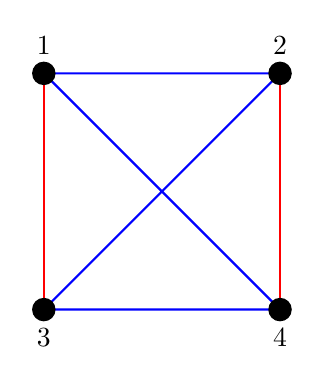
\begin{tikzpicture}[thick,scale=0.5]
        \coordinate (A) at (0,6);
        \coordinate (B) at (6,6);
        \coordinate (C) at (0,0);
        \coordinate (D) at (6,0);
        \draw[blue] (A) node[black, above, yshift=3pt]{$1$}
        -- (B) node[black, above, yshift=3pt]{$2$}
        -- (C) node[black, below, yshift=-3pt]{$3$}
        -- (D) node[black, below, yshift=-3pt]{$4$}
        -- (A);
        \draw[red] (A)--(C);
        \draw[red] (B)--(D);
        \foreach \n in {A,B,C,D}
            \node at (\n)[circle,fill,inner sep=3pt]{};
    \end{tikzpicture}
\end{center}

现在,我们要如何验证同质性?需寻找三个点(三人),其所有连线均为蓝色(全友)或红色(全敌)。这正是寻找\textbf{单色三角形}的过程!(注意:三角形顶点须为原始点,而非连线交点;术语\emph{单色 (monochromatic)} 源于希腊语 \emph{monos} 和 \emph{khroma},分别表示``一个''和``颜色''。)这种表示法更直观且便于快速检验。

根据上图,我们解决了四人问题:存在一种朋友/敌人的特定配置关系,使得其中不存在全友或全敌的三人子集。这表明四人群体可能避免同质性,故无法\emph{保证}四人中必然存在同质子集。

能否构造另一种满足该性质的配置?如何判断其与已有配置\emph{不同}?满足条件的配置共有多少种?现在请尝试构造一个\emph{必然存在}同质三人子集的配置——其形态如何?此类配置又有多少种?

\subsubsection*{重述 $n = 5$ 的问题}

让我们继续思考由五个人组成的小组。我们的图需要调整,因为现在有五个点,这意味着需要绘制更多的线。尽管如此,我们仍会用蓝色或红色线填充所有连线,并确保没有单色三角形。这可能吗?(提示:尝试将点排列成规则五边形,然后填充连线。)尝试几次,看看你的排列是否有效。随机添加几条线,并通过确保新线不会形成单色三角形来指导你的选择,这也可能有帮助。

你做出来了吗?翻页看看我们是如何做的……

\clearpage

\subsubsection*{解答:$n=5$}

这是我们在五个点之间连线的红/蓝线配置,完全避免了同质性:

\begin{center}
    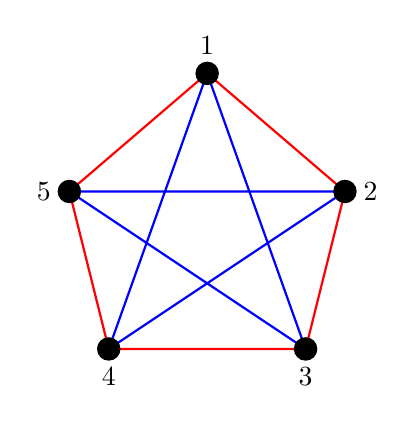
\begin{tikzpicture}[thick,scale=0.5]
        \coordinate (A) at (0,0);
        \coordinate (B) at (5,0);
        \coordinate (C) at (6,4);
        \coordinate (D) at (2.5,7);
        \coordinate (E) at (-1,4);
        \draw[red] (A) node[black, below, yshift=-3pt]{$4$}
        -- (B) node[black, below, yshift=-3pt]{$3$}
        -- (C) node[black, right, xshift=3pt]{$2$}
        -- (D) node[black, above, yshift=3pt]{$1$}
        -- (E) node[black, left, xshift=-3pt]{$5$}
        -- (A);
        \draw[blue] (A)--(D)--(B)--(E)--(C)--(A);
        \foreach \n in {A,B,C,D,E}
            \node at (\n)[circle,fill,inner sep=3pt]{};
    \end{tikzpicture}
\end{center}

请注意该图形优雅的对称性:所有红线均位于五边形的外侧,所有蓝线均位于图形内部。原因是,任意三个相邻点构成的三角形必须使用两条外线和一条内线,而任意三个不相邻点构成的三角形必须使用两条内线和一条外线。(想一想:为什么我们不能用三条内线或三条外线组成一个三角形?)这\emph{保证}了我们构成的任何三角形都会使用两种不同颜色的线,所以这个图形没有单色三角形!当然,我们可以检查图中所有可能的三角形,并确保它们都不是单色的。这样的三角形有多少个?你能多快手工找到所有这些三角形?这样做是否更容易,或者利用我们上面提到的内部/外部属性?

也许你找到的解决方案与我们的图形不同。你怎么知道它是否是不同的图形?你的图中有多少条蓝线、多少条红线?我们的图中呢?尝试通过移动点来重绘图形,但保持点之间的连接关系(即任意两点之间连线的颜色)。你能把你的图形调整得跟我们的一样吗?你认为这对本问题的解的数量意味着什么?

\subsubsection*{$n=6$ 的情况}

现在我们可以思考六个人的情况了。考虑六个点以及它们之间所有可能的连线,我们需要用蓝色或红色为每条线上色,并确保图中不存在所有边颜色相同的三角形。绘制前,请回顾四个点和五个点时我们找到的解决方案。这些解的结构如何?这次我们需要画多少条边?能否尝试构造一个与五点解相似的图形?思考当前问题与先前工作的相似之处往往大有裨益。现在,请尝试画出这个图形并观察结果。

图形是否有效?若无效,问题何在?你在何处遇到了困难?在被迫画出单色三角形之前,最多能添加多少条边?换句话说,在加入下一条必然形成单色三角形(无论颜色)的边之前,图中最多能容纳多少条边?虽然这些问题看似偏离了解决当前难题的主线,但它们本身极具启发性,并可能引导我们找到解法或其推广。为便于说明,下图展示了我们为边分配红蓝两色的一种方案。为何在此处停笔?还需添加多少条边?我们能否继续添加?

\begin{center}
    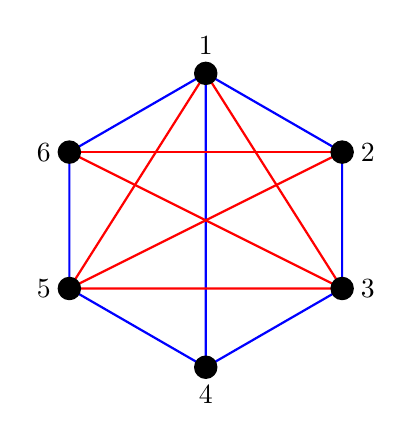
\begin{tikzpicture}[thick,scale=0.5]
        \coordinate (A) at (0,0);
        \coordinate (B) at (-3.4642,2);
        \coordinate (C) at (-3.4642,5.4642);
        \coordinate (D) at (0,7.4642);
        \coordinate (E) at (3.4642,5.4642);
        \coordinate (F) at (3.4642,2);
        \draw[blue] (A) node[black, below, yshift=-3pt]{$4$}
        -- (B) node[black, left, xshift=-3pt]{$5$}
        -- (C) node[black, left, xshift=-3pt]{$6$}
        -- (D) node[black, above, yshift=3pt]{$1$}
        -- (E) node[black, right, xshift=3pt]{$2$}
        -- (F) node[black, right, xshift=3pt]{$3$}
        -- (A)
        -- (D);
        \draw[red] (B)--(E);
        \draw[red] (C)--(F);
        \draw[red] (B)--(D)--(F)--(B);
        \draw[red] (C)--(E);
        \foreach \n in {A,B,C,D,E,F}
            \node at (\n)[circle,fill,inner sep=3pt]{};
    \end{tikzpicture}
\end{center}

我们面临的局面颇具深意,因其性质与先前情况截然相反。在四点与五点情形中,我们试图证明\emph{可以}通过边的着色方案避免单色三角形——只需构造出满足条件的\emph{具体}图形即可证明其存在性。然而对于六个点,似乎无法通过边的着色避免单色三角形。如何证明这一结论?最直接的想法是枚举所有可能的着色方案,并论证每种方案下至少存在一个单色三角形。这可行吗?着色方案共有多少种?如何在给定图形中快速定位单色三角形?回忆我们如何处理五点图形:我们注意到任何三角形必须包含\emph{至少}一条外部边与\emph{至少}一条内部边,这保证了三角形必含两种颜色的边。能否在此采用类似思路,确立某种\emph{必然}导致单色三角形存在的性质?

问题在于,六个点构成的图形中边的着色方案数量过于庞大,难以手动穷尽!图中需着色的边共有 $15$ 条,每条边可选红蓝两色,因此共有 $2^{15}$ 种着色方案——这是一个天文数字!(实际同构类会略少,因为部分方案在某种意义上是等价的;更专业地说,它们是``\emph{同构的}''。)

\subsubsection*{解答:处理\emph{任意}图形}

我们需要更巧妙的方法来论证,以便在不绘制特定图形的情况下证明\emph{任意}图形的性质。也就是说,我们需要找到对所有可能的六点图形都成立的事实,并据此推断出必然存在单色三角形。一种解决思路是关注图形的局部结构。具体而言,任取六个点中的一个,考虑从该点引出的五条边。例如,我们可能得到如下图形:

\begin{center}
    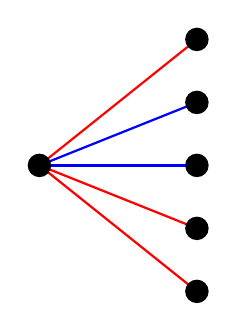
\begin{tikzpicture}[thick,scale=0.2]
        \coordinate (A) at (-6,0);
        \coordinate (B) at (4,4);
        \coordinate (C) at (4,0);
        \coordinate (D) at (4,8);
        \coordinate (E) at (4,-4);
        \coordinate (F) at (4,-8);
        \draw[blue] (A)--(C);
        \draw[blue] (A)--(B);
        \draw[red] (A)--(D);
        \draw[red] (A)--(E);
        \draw[red] (A)--(F);
        \foreach \n in {A,B,C,D,E,F}
            \node at (\n)[circle,fill,inner sep=3pt]{};
    \end{tikzpicture}
\end{center}

有多少条蓝边,多少条红边?这有些棘手:我们并非针对任何\emph{特定}图形(如上图),而是寻求适用于所有可能图形的结论。因此无法给出具体答案。面对一个\textbf{任意}图形,我们必须构建一个普遍有效的论证。

关键点在于:从该点出发的五条边中,必有三条同色(蓝或红)。试想,若非如此,则蓝边不超过两条,红边也不超过两条,总计最多四条边。但实际有五条边!(这是``\emph{抽屉原理}''的典型应用:无法将五个物体按两种颜色分类,而不使某一颜色达到三个。该原理是解决此类问题的有力工具,详见 \ref{sec:section8.6} 节。)

至此,我们得到了什么?从任意一个六点完全图中选定一点,该点必引出三条同色边。颜色可能为红或蓝,因此不能假定仅为红色;若假设为红色进行论证,之后还需讨论蓝色情况。为简化,我们首先分析从该点引出三条红边的情况(暂不限定其他边的颜色):

\begin{center}
    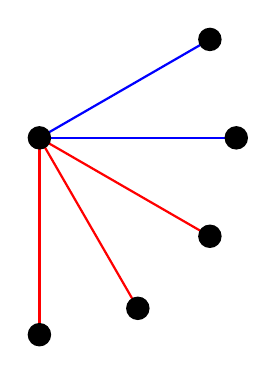
\begin{tikzpicture}[thick,scale=0.5]
        \coordinate (A) at (0,0);
        \coordinate (B) at (4.33,2.5);
        \coordinate (C) at (5,0);
        \coordinate (D) at (4.33,-2.5);
        \coordinate (E) at (2.5,-4.33);
        \coordinate (F) at (0,-5);
        \draw[blue] (A)--(C);
        \draw[blue] (A)--(B);
        \draw[red] (A)--(D);
        \draw[red] (A)--(E);
        \draw[red] (A)--(F);
        \foreach \n in {A,B,C,D,E,F}
            \node at (\n)[circle,fill,inner sep=3pt]{};
    \end{tikzpicture}
\end{center}

现在,如何添加剩余边才能避免三点间出现同色三角形?由于未限定孤立点之间边的颜色,我们聚焦于底部的三个点。它们之间的边可能是什么颜色?若其中任一条为红色,则其两个端点与原始点便构成红色三角形!这就有问题了。

\begin{center}
    \begin{tikzpicture}[thick,scale=0.5]
        \coordinate (A) at (0,0);
        \coordinate (B) at (4.33,2.5);
        \coordinate (C) at (5,0);
        \coordinate (D) at (4.33,-2.5);
        \coordinate (E) at (2.5,-4.33);
        \coordinate (F) at (0,-5);
        \draw[blue] (A)--(C);
        \draw[blue] (A)--(B);
        \draw[red] (A)--(D);
        \draw[red] (A)--(E);
        \draw[red] (A)--(F);
        \draw[red] (E)--(F);
        \draw [red,-stealth,very thick] (-2,-2.4) node[red, above]{$\text{红色三角形}$} -- (1,-3.5);
        \foreach \n in {A,B,C,D,E,F}
            \node at (\n)[circle,fill,inner sep=3pt]{};
    \end{tikzpicture}
\end{center}

避免此情况的唯一方法是将这三条边全染为蓝色。但此时,这三个点之间就形成了蓝色三角形!可见无论如何操作,都无法避免单色三角形!

\begin{center}
    \begin{tikzpicture}[thick,scale=0.5]
        \coordinate (A) at (0,0);
        \coordinate (B) at (4.33,2.5);
        \coordinate (C) at (5,0);
        \coordinate (D) at (4.33,-2.5);
        \coordinate (E) at (2.5,-4.33);
        \coordinate (F) at (0,-5);
        \draw[blue] (A)--(C);
        \draw[blue] (A)--(B);
        \draw[red] (A)--(D);
        \draw[red] (A)--(E);
        \draw[red] (A)--(F);
        \draw[blue] (F)--(D)--(E)--(F);
        \draw [blue,-stealth,very thick] (5.5,-3.8) node[blue, right]{$\text{蓝色三角形}$} -- (2.5,-3.8);
        \foreach \n in {A,B,C,D,E,F}
            \node at (\n)[circle,fill,inner sep=3pt]{};
    \end{tikzpicture}
\end{center}

现在回到抽屉原理的初始结论。若原理保证的三条同色边是蓝色而非红色呢?论证结构完全一致:观察底部三点间的边,

\begin{center}
    \begin{tikzpicture}[thick,scale=0.5]
        {
            \coordinate (A) at (0,0);
            \coordinate (B) at (4.33,2.5);
            \coordinate (C) at (5,0);
            \coordinate (D) at (4.33,-2.5);
            \coordinate (E) at (2.5,-4.33);
            \coordinate (F) at (0,-5);
            \draw[red] (A)--(C);
            \draw[red] (A)--(B);
            \draw[blue] (A)--(D);
            \draw[blue] (A)--(E);
            \draw[blue] (A)--(F);
            \draw[blue] (E)--(F);
            \draw [blue,-stealth,very thick] (-2,-2.4) node[blue, above]{$\text{蓝色三角形}$} -- (1,-3.5);
            \foreach \n in {A,B,C,D,E,F}
                \node at (\n)[circle,fill,inner sep=3pt]{};
        }
        {
            \coordinate (A1) at (8,0);
            \coordinate (B1) at (12.33,2.5);
            \coordinate (C1) at (13,0);
            \coordinate (D1) at (12.33,-2.5);
            \coordinate (E1) at (10.5,-4.33);
            \coordinate (F1) at (8,-5);
            \draw[red] (A1)--(C1);
            \draw[red] (A1)--(B1);
            \draw[blue] (A1)--(D1);
            \draw[blue] (A1)--(E1);
            \draw[blue] (A1)--(F1);
            \draw[red] (F1)--(D1)--(E1)--(F1);
            \draw [red,-stealth,very thick] (13.5,-3.8) node[red, right]{$\text{红色三角形}$} -- (10.5,-3.8);
            \foreach \n in {A1,B1,C1,D1,E1,F1}
                \node at (\n)[circle,fill,inner sep=3pt]{};
        }
    \end{tikzpicture}
\end{center}

若添加任何蓝边,会与原始点形成蓝色三角形;若全染红色,则三点间形成红色三角形!因此,无论最初的三条同色边是红色还是蓝色,论证过程完全\emph{对称}。数学家常利用这种对称性简化证明,表述为``不失一般性,假设三条边为红色''。这意味着,若选择蓝色,后续论证在数学结构上完全相同,故无需重复书写。实际上,这种情况非常常见,以至于``不失一般性''这个术语有时会缩写为 \textbf{WOLOG} 或 \textbf{WLOG} (without loss of generality)。

\subsubsection*{解答:结果总结}

截至目前我们取得了哪些进展?我们绘制了\emph{特定}图形,证明在四个或五个点之间可以着色连线而不形成单色三角形,同时推断\emph{任意}六个点构成的图形\emph{必然}包含单色三角形。对应回原始问题的朋友/敌人表述,这意味着任意六人群体中都存在一个三人组,其成员要么全部互为朋友,要么全部互为敌人。

值得注意的是,将问题转化为点线模型极具启发性;它使我们完全脱离可能分散注意力的社交背景,并简化了术语体系——将人际关系标记简化为两点间的连线。这是极具价值的解题策略:提炼问题的核心结构(底层逻辑、元素间关系及其相互作用),并据此重构表述。这种方法不仅使复杂问题更易于理解和处理,还能指导我们建立更优的符号系统。试想若坚持使用``$13F, 23E, \dots$''这类符号进行推演,也许最终也能求解,但过程必将困难重重!

原题核心目标之一是确定满足特性的最小群体规模。我们是否已完成此目标?六是否为该下界?在任意七人群体中,必然包含六人子群,而前述结论表明该子群中必定存在同质三人组(全友或全敌)。此性质自然推广至更大规模的群体,因此六确实为所求的精确下界。这与匈牙利社会学家在四人子群中观察到的现象类似,而当前问题因规模更大而显著复杂化——我们实际解决的是更小规模的简化案例。两者均属\textbf{拉姆齐理论}范畴,该组合数学与图论分支致力于探寻此类``下界规律'':当结构(如人群)规模增长至临界点时,\emph{必然}出现具备特定性质的子结构(如全友/全敌三人组)。这一始于社会现象的研究,最终被严格证明为数学定理。多么奇妙啊!

\subsubsection*{泛化:留给你的问题}

在继续之前,让我们提出一些有趣且相关的问题。如果我们要寻找不同规模的同质子群(例如四人、五人或十二人)该怎么办?一般来说,我们必须有更多的人才能保证找到这样的子群。我们能否总是这样做?也就是说,给定任何所需的子群大小,我们能否像之前那样确定一个下界?即使没有找到具体的数字,你能想出证明这种下界存在的方法吗?此外,如果我们允许第三种可能性:朋友、敌人或陌生人,又会怎样?我们能否回答关于同质子群的类似问题?这些都与拉姆齐理论相关,其中一些问题非常困难,需要数学家多年努力才能解决。许多看似简单的问题至今仍悬而未决!如果你在这些问题上没有进展,请不要灰心。我们相信,任何尝试和思考都是有意义且有益的。

\subsubsection*{解题心得}

这个问题的解决涉及几个难点。首先,我们必须找到一种方式来有效地解释谜题,以便解决问题,这涉及引入适当的符号来表示元素。这是解决数学问题的重要部分,尤其是当问题本身不提供符号或可视化时。

其次,为了确定六是群规模的下界,我们必须证明某些情况是不可能的,但可能的情况数量太多,无法逐一检验。这种情况在计算机科学和算法问题中尤其常见。为了解决这个问题,我们必须采用比大力出奇迹更巧妙的策略,但策略的选择并不总是显而易见的。在这里,我们尝试添加连接线,但最终意识到无法继续推进。证明某件事是可能的,只需提供一个例子(如我们对四人和五人组所做的那样),但证明某件事是不可能的则要复杂得多,需要针对具体情境的独创性。

最后,我们发现思考与当前问题密切相关的问题很有趣,这些问题通常只需调整原问题的一个或多个条件。如果我们寻找更大的子群怎么办?如果我们允许更多类型的连接怎么办?这将如何改变结果?通过改变这些条件来探索问题的边界,可以带来新的数学发现和技术,激励数学家积极探寻新知识并分享方法。


% !TeX root = ../../../book.tex
\subsection{三门问题}

\subsubsection*{问题描述}

这个问题仅涉及基础概率与算术,但多年来却让无数聪明人折戟沉沙。1990 年,玛丽莲·沃斯·萨万特 (Marilyn vos Savant) 在《Parade》杂志专栏发表该问题及其解法后,引发了激烈争论,许多人(包括数学家)致信赞同或反对她(正确)的答案。让我们看看你的见解!

\begin{quote}
    假设你正在参加一档游戏节目,面前有三扇门。其中一扇门后是汽车,其余两扇后是山羊。游戏开始前,汽车和山羊的位置已被随机放置在门后。游戏规则如下:你选定一扇门后,该门暂时保持关闭。主持人蒙蒂·霍尔 (Monty Hall) 知晓门后的情况,他会打开其余两扇门中有山羊的一扇。若两扇门后皆为山羊,他会随机开启一扇。蒙蒂·霍尔打开一扇有山羊的门后,会询问你:是坚持最初的选择,还是切换至另一扇关闭的门?试想:你选择了 1 号门,主持人打开了藏有山羊的 3 号门,然后问你:``是否要换到 2 号门?''改变最初的选择对你有利吗?
\end{quote}

当然,我们假设你更希望赢得汽车而非山羊,且力求最大化获胜概率。值得一提的是,该问题得名于电视节目《\emph{Let's Make a Deal}》的主持人蒙蒂·霍尔 (Monty Hall)。

那么你怎么想?试想自己站在聚光灯下,面对所有观众,当蒙蒂·霍尔问你:``要换到另一扇门吗?'' 你会作何选择?

请仔细思考一下,然后再翻页阅读解答。

\clearpage

\subsubsection*{结论:\emph{坚决}切换}

我们直接给出结论——该结论可能令人惊讶:你应当改变最初的选择!推理过程才是棘手且令人困惑的部分,而如何建立正确的解题思路正是该问题长期困扰求解者的原因。

\subsubsection*{错误论证分析}

首先展示一个常见的错误``解答'',该解答声称换门与否无关紧要。假设你与朋友讨论此题时对方提出如下解释,你会如何回应?该论证是否成立?若不同意,你会如何指出其谬误?

\begin{quote}
    当我选定一扇门后,蒙蒂·霍尔展示了另一扇有山羊的门,此时只剩两扇关闭的门。一扇后有山羊,另一扇后有汽车,因此我最初选择的门后有汽车的概率为 $50\%$,另一扇门后有汽车的概率也为 $50\%$。因此,换门不换门没有区别,还不如坚持最初的选择。
\end{quote}

上面的解释能说服你吗?让我们揭示其根本缺陷。解决此问题的关键在于计算两个概率值:坚持原选择获胜的概率,以及换门后获胜的概率。唯有准确计算并比较这两个值,才能彻底解决这个难题。

上述论证将两个概率均视为 $50\%$,但其推理存在根本缺陷。你认为坚持原选择获胜的真实概率是多少?关键在于:展示有山羊的门的行为并不会影响最初选择的门后的物体。请重点理解以下陈述:

\begin{quote}
    因为有三扇门,所以一开始选择正确的门的概率是 $\frac{1}{3}$,看到另一扇门后面有山羊\emph{并不能改变这一事实}。
\end{quote}
这正是上面错误论证的核心症结,也是``解答''本题时最常见的误区。

接下来计算换门后的胜率,并将其与 $\frac{1}{3}$ 进行比较。事实上,有多种方法可以计算此概率。一种简洁的推导是:只要初始选择的门后是山羊(概率 $\frac{2}{3}$),换门必然获胜(赢得汽车)。因为此时两扇未选门中藏着山羊与汽车,主持人必定展示有山羊的门,剩余那扇门后必定是汽车。因此换门策略的胜率为 $\frac{2}{3}$。

\subsubsection*{枚举可能性}

上述解释可能无法令你信服,我们不妨尝试实际枚举门后山羊与汽车的可能排列,并具体分析每种情况下切换选择的结果。首先请注意,门的编号并无实质影响,因为所有选择都是随机的;也就是说,无论汽车停在 1 号门、2 号门还是 3 号门后,我们最初选中汽车的概率始终是 $\frac{1}{3}$。因此可 \textbf{WOLOG}(此缩写意为``不失一般性'')假设汽车位于 1 号门后,山羊分别在 2 号门和 3 号门后。需要强调的是,这是我们自己设定的条件,参赛者并不知晓(否则必然直接选择 1 号门!)。基于此设定,我们考察初始选择的全部三种情况:

\begin{center}
    \begin{tabular}{ c|c|c } 
     1 号门 & 2 号门  & 3 号门 \\ 
     \hline 
     汽车   & 山羊    & 山羊 \\
    \end{tabular}
\end{center}

\begin{center}
    \begin{tabular}{ c|c|c|c } 
     我们的选择 & 主持人展示 & 换门结果 & 不换门结果 \\ 
     \hline 
     1 号门    & 2 号门 \:或\: 3 号门  & 山羊 & 汽车 \\
     2 号门    & 3 号门            & 汽车 & 山羊 \\
     3 号门    & 2 号门            & 汽车 & 山羊 \\
    \end{tabular}
\end{center}

关键发现在于:当我们初始选中有汽车的门时,主持人可以随机开启任意一扇有山羊的门。但无论开启哪扇门,切换选择都将失败,而坚持选择会获胜。这种情况仅占 $\frac{1}{3}$,即初始选中汽车的概率。由于表中所有情况概率均等,可以得出结论:切换策略的胜率为 $\frac{2}{3}$,而坚持策略的胜率仅为 $\frac{1}{3}$。

现在是否感觉问题更清晰了?不妨向亲友提出这个问题并观察他们的反应:有多少人答对?多少人能正确解释?多少人误答``概率相同''?又有多少人此前已经接触过此题?

\subsubsection*{泛化到多门多车情形}

让我们将这个游戏节目问题泛化,分析切换策略是否仍然有效。假设共有 $n$ 扇门和 $m$ 辆汽车,因此有 $n - m$ 只山羊。为进行有效分析,需满足 $m \le n - 2$,原因如下:

\begin{itemize}
    \item 如果 $m = n$,则无论切换与否都必然获胜,无需讨论。
    \item 如果 $m = n-1$,当初始选择有山羊的门时,主持人\emph{无法}展示另一扇有山羊的门,游戏规则无法成立,切换策略也就毫无意义。
\end{itemize}

现在,有了这些变量,游戏的新规则如下:我们随机选择一扇门。主持人从\emph{其余}门中随机打开一扇有山羊的门。此时可选择坚持最初选择或切换至\emph{任意}未打开的门。关键问题是:最优策略是什么?切换是否有利?答案是否取决于 $m$ 和 $n$?

我们将用与原题中第一种方法大致相同的方式来处理这道修改后的问题。由于 $m,n$ 为变量,我们无法枚举所有情况,只能采用逻辑推理来推断坚持和切换的胜率。首要观察与原始问题一致:\emph{坚持策略}的胜率等于初始选中汽车的概率。若初始选中有汽车的门(概率 $\frac{m}{n}$),坚持必胜;若选中有山羊的门(概率 $\frac{n-m}{n}$),坚持必败。故坚持策略的胜率为 $\frac{m}{n}$。

为了计算切换策略的胜率,需要分两种情况讨论。请注意,当 $m \geq 2$ 时,初始选中有汽车的门后切换仍可能获胜。考虑到这一点,我们需要分两种不同情况讨论:(a) 初始选中有山羊的门的情况,(b) 初始选中有汽车的门的情况。每种情况都会给主持人留下不同数量的选择,进而留下不同数量的切换策略和获胜方式,所以此处需要分开处理。

\begin{enumerate}[label=(\alph*)]
    \item \textbf{初始选中有山羊的门}。现在还剩下 $n - m - 1$ 扇有山羊的门,主持人随机选择其中一扇打开。从我们的角度来看,切换给我们留下了 $n-2$ 个选项(我们不能切换到已打开的门和最初选择的门),其中 $m$ 个是汽车。因此,在这种\emph{特定}情况下,切换后获胜的概率为 $\frac{m}{n-2}$。\\
    由于最初有 $n - m$ 只山羊,所以这种情况发生的概率为 $\frac{n-m}{n}$。因此,这种情况对切换后总获胜概率的贡献为
    \[\frac{n-m}{n} \cdot \frac{m}{n-2} = \frac{nm-m^2}{n(n-2)}\]
    (思考一下为什么我们要把这些概率相乘而不是相加?我们要如何将此概率与下一种情况的概率结合起来?)
    \item \textbf{初始选中有汽车的门}。现在还剩下 $n - m$ 扇有山羊的门,主持人随机选择其中一扇打开。从我们的角度来看,切换给我们留下了 $n-2$ 个选项,其中 $m - 1$ 个是汽车。因此,在这种\emph{特定}情况下,切换后获胜的概率为 $\frac{m-1}{n-2}$。\\
    由于最初有 $m$ 辆车,所以这种情况发生的概率为 $\frac{m}{n}$。因此,这种情况对切换后总获胜概率的贡献为
    \[\frac{m}{n} \cdot \frac{m-1}{n-2} = \frac{m^2-m}{n(n-2)}\]
\end{enumerate}

由于这两种情况是独立发生的(即它们不可能同时发生),我们需要将这两个概率相加,从而得到切换策略的总胜率:
\begin{align*}
    \frac{nm-m^2}{n(n-2)} + \frac{m^2-m}{n(n-2)} &= \frac{nm - m^2 + m^2 - m}{n(n-2)} \\
    &= \frac{nm - m}{n(n-2)} \\
    &= \frac{m(n - 1)}{n(n-2)} \\
    &= \frac{m}{n} \cdot \frac{n-1}{n-2}
\end{align*}
将此结果与坚持策略的胜率 $\frac{m}{n}$ 比较。因为 $ n - 1 > n - 2$,所以 $\frac{n-1}{n-2} > 1$,可得不等式:
\[\frac{m}{n} < \frac{m}{n} \cdot \underbrace{\frac{n-1}{n-2}}_{>1}\]
切换策略的胜率\emph{严格大于}(即总是大于)坚持策略的胜率。因此,随机切换到另一扇门总是更优策略!

\subsubsection*{具体应用}

此问题的原始版本对应 $n = 3$ 且 $m = 1$,因此可以将这些值代入来验证结果的正确性。根据推导公式,坚持策略的胜率为 $\frac{1}{3}$,而切换策略的胜率为 $\frac{1(3-1)}{3(1)} = \frac{2}{3}$,与之前的结论完全吻合!

\subsubsection*{泛化:留给你的问题}

当 $m$ 和 $n$ 取其他值时会发生什么?能否使``始终切换''策略显著优于``始终坚持''策略?两种策略的胜率差异最大能达到多少?最小又能缩小至何种程度?是否存在使两者胜率相等的情况?

该问题的另一变体是主持人开启多于一扇有山羊的门。具体设定如下:共有 $n$ 扇门,其中 $m$ 扇后有汽车;玩家首次选择后,主持人从剩余门中随机开启 $p$ 扇有山羊的门;此时玩家可选择坚持初始选择,或切换到未开启的 $n-p-1$ 扇门中的任意一扇。在此情形下最优策略是什么?需对 $m,n,p$ 施加何种约束条件以保证游戏成立?最优策略是始终切换,还是取决于 $p$ 的取值?``始终切换''与``始终坚持''策略的胜率差异范围如何?

\subsubsection*{解题心得}

直觉和快速决策有时能\emph{引导}我们找到正确答案,但务必检查这些仓促判断是否基于合理的逻辑。本题中,``$50/50$''的概率初看似乎成立,但仔细推敲后便发现其论证存在缺陷——关键在于正确解读题目并严格遵循游戏步骤的顺序。概率分析应按照游戏实际发生的流程进行,而非从结果倒推。

概率问题往往极具迷惑性,需格外审慎对待。这也揭示了一个深刻启示:看似简单的问题往往最难攻克。切勿因表述简短或易于理解而轻视问题的复杂性!

关于蒙蒂·霍尔问题及其心理学背景,请参见 \href{http://www.usd.edu/~xtwang/Papers/MontyHallPaper.pdf}{Krauss, Stefan and Wang, X. T. (2003). ``The Psychology of the Monty Hall Problem: Discovering Psychological Mechanisms for Solving a Tenacious Brain Teaser'', \emph{Journal of Experimental Psychology}: General 132(1)}。

\newpage
% !TeX root = ../../../book.tex
\section{学而时习之}\label{sec:section1.5}

我们以一些练习来结束本章,这些练习既包含了我们讨论过的一些想法,又给了你一个机会来实践之前所学,抑或只是为了让你保持思维敏捷。尽可能多地尝试,并与朋友们讨论可能的解决方案,看看他们的想法。不过,归根结底,把这些练习当作一种保持大脑灵活的方式就好!

\begin{exercise}
    一只苍蝇停在一辆以每小时 $60$ 公里的速度向前疾驰的火车前面。在同一条轨道上,前方 $300$ 公里处,另一列火车正以每小时 $60$ 公里的速度向前一列火车疾驰而来。此时,当火车相距 $300$ 公里时,苍蝇以每小时 $90$ 公里的速度起飞,不断地在火车之间的轨道上方来回飞行,到达火车时瞬间转身。在两列火车相撞,挤压到它们之间苍蝇之时,苍蝇总共飞了多少距离?你是怎么想出来的?尝试将情况泛化到一列火车以 $a$ km/hr 行驶,另一列以 $b$ km/hr 行驶,而苍蝇以 $c$ km/hr 飞行。
\end{exercise}

\begin{exercise}
    政府铸币厂受委托铸造一批金币。铸币厂有 $20$ 台机器,每台机器生产重 $5$ 克的硬币。一天,铸币厂的工头发现有些硬币轻了,他对机器进行了盘查,发现其中一台机器铸造出的硬币为 $4$ 克,而其他 $19$ 台机器工作正常。他决定化不利为有利,以此找到最聪明的员工,接下来提拔他。他告诉工人,只有一台机器正在生产 $4$ 克的硬币,他们需要确定哪台机器坏了。作为员工,你可以在秤上称一次,但\emph{只能}称一次。你可以放置任意选定机器生产的任意数量的硬币,但必须将它们放置在一起,并且只会看到所有硬币的总重量,以克为单位。你要如何做,才能准确地确定哪台机器坏了?
\end{exercise}

\begin{exercise}
    在国际象棋中,皇后可以垂直、水平或沿对角线任意方向移动任意数量的格子。尝试在一个标准的 $8 \times 8$ 棋盘上放置 $8$ 个皇后,使得任意皇后都不会攻击到其他皇后(也就是说,\emph{没有}皇后可以下一步立即吃掉另一个皇后)。展示一种方法来做到这一点或证明这是不可能的。如果你找到了一种方法,你认为有多少种不同的方法可以做到这一点?如果你证明这是不可能的,请找出最多多少个皇后可以满足条件。以这种方式,你最多可以在棋盘上放置多少个皇后?
\end{exercise}

\begin{exercise}
    在一个标准的 $8 \times 8$ 棋盘上,在对角处移除 $2$ 个格子,比如右上角和左下角。你能用 $2 \times 1$ 的多米诺骨牌覆盖所有剩余的方格,且所有的多米诺骨牌都不\emph{重叠}吗?(注意:这被称为棋盘\emph{密铺}。)为什么能或为什么不能?在一般情况下,如果有一个 $n \times n$ 棋盘呢?你的答案取决于 $n$ 吗?为什么会这样呢?
\end{exercise}

\begin{exercise}
    考虑一个标准的 $8 \times 8$ 棋盘,对角上移除两个相邻的方块。(如图。)你能用 T 形四联骨牌密铺这个棋盘吗?(如图。)如果可以,怎么做到?如果不能,为什么不能?

    \begin{center}
        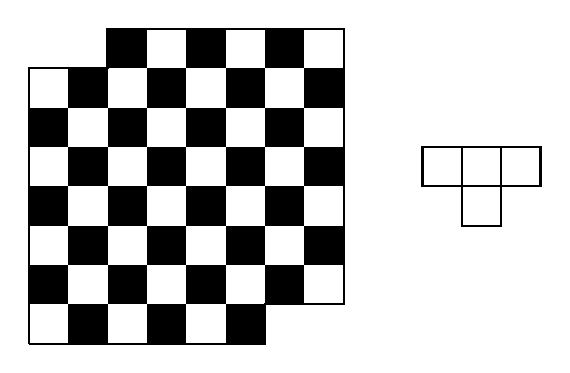
\begin{tikzpicture}[thick, scale=0.5, x=1cm]
            \foreach \x in {0,...,5}
                {
                    \pgfmathparse{mod(\x,2) ? "black" : "white"}
                    \edef\colour{\pgfmathresult}
                    \path[fill=\colour] (\x, 0) rectangle ++ (1,1);
                }
            \foreach \x in {0,...,7} 
                \foreach \y in {1,...,6}
                    {
                        \pgfmathparse{mod(\x+\y,2) ? "black" : "white"}
                        \edef\colour{\pgfmathresult}
                        \path[fill=\colour] (\x,\y) rectangle ++ (1,1);
                    }
            \foreach \x in {2,...,7}
                {
                    \pgfmathparse{mod(\x+1,2) ? "black" : "white"}
                    \edef\colour{\pgfmathresult}
                    \path[fill=\colour] (\x, 7) rectangle ++ (1,1);
                }
            \draw (0,0)--(6,0)--(6,1)--(8,1)--(8,8)--(2,8)--(2,7)--(0,7)--(0,0);
            \draw (10,4) rectangle ++ (1,1);
            \draw (11,4) rectangle ++ (1,1);
            \draw (12,4) rectangle ++ (1,1);
            \draw (11,3) rectangle ++ (1,1);
        \end{tikzpicture}
    \end{center}

    一般情况下,如果是 $n \times n$ 棋盘呢?你的答案取决于 $n$ 吗?为什么会这样呢?
\end{exercise}

\begin{exercise}
    给定一个实数 $x$,我们令 $\lfloor x \rfloor$ 表示小于(或等于)$x$ 的最大整数,让 $\lceil x \rceil$ 表示大于(或等于)$x$ 的最小整数。例如,$\lfloor 6.02 \rfloor = 6$, $\lfloor 6.99999 \rfloor = 6$, $\lfloor 6 \rfloor = 6$, $\lfloor -6.5 \rfloor = -7$ 。

    尽可能为以下表达式的值确定更具体和简洁的表示形式。(你可能需要找到一些不同的表达式,具体取决于 $x$。)

    \begin{enumerate}
        \item $\lfloor x \rfloor + \lfloor 1-x \rfloor$ 
        \item $\lceil x \rceil + \lceil 1-x \rceil$
        \item $\lfloor x \rfloor + \lceil x \rceil$
        \item $\frac{\lfloor x \rfloor}{x}$
        \item $\lfloor x^2 \rfloor - \lfloor x \rfloor ^2$
        \item $\lceil x^2 \rceil - \lceil x \rceil^2$
    \end{enumerate}
\end{exercise}

\begin{exercise}
    求三个自然数 $a,b,c$,使得没有子集的和能被 $3$ 整除。即求 $a,b,c$,使得下列和都不能被 $3$ 整除:$a,b,c,a + b,a + c,b + c,a + b + c$。这可能吗?为什么能或为什么不能?

    尝试用 $4$ 个数做同样的事情:求自然数 $a,b,c,d$,使得没有子集的和能被 $4$ 整除。这可能吗?为什么能或为什么不能?

    尝试泛化一下,你能说一说找到 $n$ 个自然数使得所有子集的和都不能被 $n$ 整除吗?
\end{exercise}

\begin{exercise}
    回想一下我们通过点和彩色线条解决朋友趋势问题的方法。对于这个问题,我们想解决类似的情况,我们有一定数量的点,需要绘制所有可能的线,让任意两点都恰好由一条线连接,但在这种情况下,我们不关心颜色,所以我们可以说所有的线都是黑色的。你能用 $3$ 个点画出这个图形,使所有的线都不交叉吗?$4$ 个点呢?$5$ 个?$6$ 个?为什么行或者为什么不行?试着解释为什么这些图形中的任何一个都不可能实现。如果你不能实现 $0$ 次交叉,你可能达到的最小数量是多少?
\end{exercise}

\begin{exercise}
    画一个圆圈。沿圆周放置 $3$ 个点。我们想给点之间的部分着色(每个部分只有一种颜色),两个相同颜色不相邻。我们需要多少种颜色?如果我们在圆周上放置 $4$ 个点呢?$5$ 个呢?尝试泛化到 $n$ 个点。你能说一下所需的颜色数量吗?
\end{exercise}

\begin{exercise}
    假设你有一个装满袜子的抽屉。里面有 $2$ 双蓝色袜子、$3$ 双红色袜子和 $4$ 双绿色袜子。(同时假设左袜子和右袜子是无法区分的。)一天早上,你很着急,开始随机抓袜子,一次抓一只,将所有袜子拿在手上,直到你有一双为止。你需要从抽屉里拿出多少只袜子才能\emph{保证}你手上有一双袜子?

    如果每种颜色的袜子是以前的两倍,您的答案会有什么变化?如果我们每种颜色有 $3$ 双袜子,颜色分别是红色、绿色、蓝色、黄色和棕色,会怎样?如果我们每种颜色有 $n$ 双袜子,共有 $m$ 种颜色,又会怎样?
\end{exercise}

\begin{exercise}
    深夜,一行四人在回家路上来到了桥头。这座桥又旧又晃,一起过去不安全。他们只有一个手电筒,光线的强度只能同时为两个人照亮道路。每个人对这座桥的舒适程度不同,所以他们会以不同的速度过桥。一人过桥需要 $5$ 分钟,一人需要 $10$ 分钟,一人需要 $15$ 分钟,一人需要 $20$ 分钟。如果两个人一起过桥,就按照较慢的人的步调通过。四人全部过桥需要多长时间?你能找到给出绝对最短时间的方法吗?
\end{exercise}

\begin{exercise}
    考虑美元硬币的常见面额:$1$ 美分、$5$ 美分、$10$ 美分和 $25$ 美分。你需要在口袋里随身携带什么硬币才能\emph{保证}你可以准确地支付 $0$ 美分到 $100$ 美分之间的任何价格?是否有几组可能的硬币可以实现这一目标?具有此属性的硬币的最小总价值是多少?是否有几组可能的硬币具有相同的最小总值?
\end{exercise}

\begin{exercise}
    设 $a,b,c$ 为实数,其中 $a \ne 0$。以下``伪证明'' $-\frac{b}{2a}$ 是方程 $ax^2 + bx + c = 0$ 的解(如果有的话)有什么问题?

    \textbf{``伪证明'':}设 $x$ 和 $y$ 为方程的解。从 $ax^2+bx+c = 0$ 中减去 $ay^2+by+c = 0$ 得 $a(x+y)(x-y)+b(x-y) = 0$。因此,$a(x+y)+b = 0$,所以 $x + y = -ba$。因为 $x$ 和 $y$ 是\emph{任意}解,我们可以用 $x = y$ 重复这个计算。因此,$2x = -ba$,因此 $x = -2ba$ 是一个解。``$\square$''
\end{exercise}

\begin{exercise}
    解释为什么 $(-1)(-1) = 1$。假设你正在为一位对此事实持怀疑态度并需要被说服的具有相同智力水平的同学撰写证明。仅仅说``因为它就是这样!''是\emph{不够的}。试着想出一个有用的\emph{几何}或\emph{物理}解释,某种令人难忘的论证。
\end{exercise}

\begin{exercise}
    对于以下方程,确定满足它们的所有实数:

    \begin{enumerate}
        \item $\vert x-2 \vert = \vert x-3\vert$
        \item $\vert 2x-1 \vert = \vert 2x-3\vert$
        \item $\vert 2x-2 \vert = \vert 2x-3\vert$
        \item $\vert x+1 \vert = \vert x-5\vert$
        \item $\vert x-1 \vert + \vert x-2 \vert = \vert x-3\vert$
    \end{enumerate}
\end{exercise}

\begin{exercise}
    \textbf{逻辑俱乐部第一规则...:}要加入逻辑俱乐部,必须决定\emph{始终}说真话或\emph{始终}说谎话。逻辑俱乐部的成员知道谁说谎,谁诚实。我不是逻辑俱乐部的成员,但我在街上遇到三名成员发表以下言论:

    \begin{itemize}
        \item 杰克:``我们三个都是骗子。''
        \item 泰勒:``我们三人中只有两人是骗子。'' 
        \item 查克:``杰克和泰勒是骗子。''
    \end{itemize}

    如果可以的话,我应该相信谁?
\end{exercise}

\begin{exercise}
    求解满足方程 $\sqrt{x - 1} = x - 3$ 的所有实数解。解释你的工作,并尝试说明为什么你的答案是\emph{唯一}答案。
\end{exercise}

\begin{exercise}
    你有两根保险丝。每个都会燃烧整整一个小时。但是,保险丝不一定相同,并且不会以恒定速率燃烧。你身上只有一个打火机和这两根保险丝。你能精确测量 $45$ 分钟吗?如果能,请解释如何实现。如果不能,请解释原因。
\end{exercise}

\begin{exercise}
    这个问题是原题的变体,其原型最早出现在 1926 年的《星期六晚邮报》上!

    三个朋友凑钱买了一大袋 \text{M\&M} 糖果。他们把盒子带回了他们的公寓,并决定第二天在聚会上分享这袋糖果。

    夜里,第一个人醒来,想吃点零食。他决定现在就吃掉他那份糖果,第二天不吃了。他打开袋子,将 \text{M\&M} 糖果分成三等份,但发现还剩下一粒。他认为多吃一个不会有什么坏处,于是就吃掉了自己那份糖果外加多出来的那粒糖果,然后把剩下的糖果放回袋子里。

    过了一会儿,第二个人做了同样的事情。他醒来觉得肚子饿了,把袋子里剩下的糖果分成三份,吃掉了自己那份外加多出来的那粒糖果。

    又过了一会儿,第三个人也做了同样的事情,吃掉了自己那份外加多出来的那粒糖果。

    第二天聚会上,他们把剩下的糖果分成三等份并享用了。(当然,没人承认他们所做的一切)。

    一开始袋子里有多少颗 \text{M\&M} 糖果?最小可能的数字是多少?
\end{exercise}

\begin{exercise}
    给定一个实数列表,它们的\emph{算术}平均数定义为它们的总和除以项数,它们的\emph{几何}平均数定义为它们的乘积开项数次方根。也就是说,假设 $x_1, x_2, \dots , x_n$ 为实数,则算术平均数为
    \[\frac{x_1+x_2+ \dots + x_n}{n}\]
    几何平均数为
    \[\sqrt[n]{x_1 \cdot x_2 \cdot \dots \cdot x_n}\]
    (注意:一个数的 $n$ 次方根等于该数的 $\frac{1}{n}$ 次方。)

    你能找到两个数,其算术平均数和几何平均数\emph{相等}吗?你能找到两个数,其算术平均数严格大于几何平均数吗?反过来呢?

    用三个数字、四个数字等等重复此操作。您能从中识别出一般模式吗?
\end{exercise}

\begin{exercise}
    考虑不定方程 $6x+ 15y = 93$。我们想找到一些\emph{积分}解;也就是说,我们想找到满足方程的 $x$ 和 $y$ 的\emph{整数}(自然数、零和负自然数)解。

    \begin{enumerate}
        \item 找到一个解,其中 $x$ 和 $y$ 都是正整数。用几句话描述你是如何找到这个解的。
        \item 找到一个解,其中 $x$ 或 $y$ 一个值为正,另一个为负。再次说明你是如何找到个解的。
        \item 你认为有多少组解?尝试写下所有可能解的特征,或描述你是如何找到所有这些解的。
    \end{enumerate}
\end{exercise}

\begin{exercise}
    \textbf{幻方}是一个 $n \times n$ 数组,它包含从 $1$ 到 $n^2$ 的每个数字,并且具有每行和每列(以及两条主对角线)数字和为相同数字的属性。

    例如,下面是一个 $3 \times 3$ 幻方:

    \begin{center}
        \begin{squarecells}{3}
            8 & 1 & 6 \nl
            3 & 5 & 7 \nl
            4 & 9 & 2 \nl
        \end{squarecells}
    \end{center}

    请注意,在这种情况下,每行/列/对角线的所谓\textbf{幻数和}为 15。

    你能找到一个 $n \times n$ 幻方的幻数和公式吗?

    (提示:我们在本章中发现过一个有用的结论。)
\end{exercise}

\begin{exercise}
    小于或等于 $1000$ 的整数中有多少整数至少有一位为 $1$?例如 $1$、$12$ 和 $511$。
\end{exercise}

\begin{exercise}
    我们有若干堆考拉熊。为了打散它们,我们从每堆中取出一只考拉熊,然后将所有这些考拉熊放入新的一堆中。例如,如果我们从大小为 $1$、$4$ 和 $4$ 的考拉熊堆开始,那么我们将以大小为 $3$、$3$ 和 $3$ 的考拉熊堆结束;或者,如果我们从大小为 $3$ 和 $4$ 的考拉熊堆开始,我们将以大小为 $2$、$2$ 和 $3$ 的考拉熊堆结束。

    我们\textbf{有}可能\emph{只执行一次}此操作并最终得到与开始时\emph{完全相同的堆大小}(它们的顺序无关紧要;只有\emph{大小}重要)。

    确定所有具有此性质的堆的集合,并解释为什么它们是唯一的。

    \emph{提示}:具有此性质的初始情况示例是当我们只有一堆大小为 $1$ 的堆时。我们执行该操作会再次获得一堆大小为 $1$ 的堆。搞定。

    \emph{提示 2}:一定要解释为什么你的情况是\emph{唯一}有效的。我们如何确定你没有遗漏某些答案呢?
\end{exercise}

\newpage
% !TeX root = ../../../book.tex
\section{展望}\label{sec:section1.6}

本介绍性章节旨在让你思考\textbf{数学}是什么、我们如何\textbf{解决问题}以及撰写\textbf{证明}意味着什么。本书其余部分,我们将越来越详细地讨论所有这三个思想。为此,我们将探索数学世界的几个不同领域。我们对我们的旅程有一个总体计划,所以不要认为我们只是在森林中随意跌跌撞撞。我们的主要目标是 

\begin{enumerate}
    \item 将我们对数学对象的一些直觉想法形式化,
    \item 阅读大量好的证明示例并培养创建和编写好的证明的能力,
    \item 培养解决问题的能力和应用数学知识的能力,
    \item 培养对数学艺术性和科学性的欣赏。
\end{enumerate}

浏览本书开头的目录,了解我们的旅程将去向何方。这些短语和术语现在对你来说可能还很陌生,但到本书结束时,我们都会说同一种语言:\textbf{数学}。
% !TeX root = ../../book.tex
\chapter[数学归纳法]{数学归纳法:``依此类推''}\label{ch:chapter02}

% !TeX root = ../../../book.tex
\section{引言}

本章朝着更彻底地研究数学证明并学习构建我们自己的数学证明迈出了一大步,介绍了我们见到的第一个重要的\textbf{证明技术}。正如后文所述,本章旨在作为开胃菜,初尝什么是\textbf{数学归纳法}以及如何使用它。接下来的几章中,我们将严格定义归纳法并\emph{证明}该技术在数学上是可行的。没错,我们真的会去证明它如何有效以及为什么有效!不过,现在我们还要继续研究一些有趣的数学难题,这些精挑细选的问题都使用了归纳技术。

% !TeX root = ../../../book.tex
\subsection{目标}

以下简短内容将向你展示本章如何融入本书的体系。这部分内容会描述我们之前的工作将如何发挥作用,还会激发我们为什么要研究本章出现的主题,并告诉你我们的目标,以及你在阅读时应该记住什么来实现这些目标。现在,我们将通过一系列陈述为你总结本章的主要目标,以及本章结束时你应该获得的技能和知识。以下各节将更详细地重申这些想法,但这里将为你提供一个简短的列表以供将来参考。当学完本章后,请返回此列表,看看你是否理解所有这些目标。你明白为什么我们在这里概述它们很重要吗?你能定义我们使用的所有术语吗?你能应用我们描述的技术吗?

\textbf{学完本章后,你应该能够...}

\begin{itemize}
    \item 定义什么是归纳论证,以及将给出的论证分类为归纳论证或非归纳论证。
    \item 根据要解决的问题的结构来决定何时使用归纳论证。
    \item 通过类比启发式地描述数学归纳法。
    \item 通过比较和对比来识别和描述不同类型的归纳论证,并识别产生这些相似点和差异点的相应问题的基本结构。
\end{itemize}


% !TeX root = ../../../book.tex
\subsection{承上}

与上一章一样,我们仅要求读者掌握基础代数、算术及几何直观,不预设高阶数学知识。本章将频繁使用求和符号($\sum$)与求积符号($\prod$),若需复习符号系统,请参阅第 \ref{sec:section1.3.5} 节。


% !TeX root = ../../../book.tex
\subsection{启下}

回顾 \ref{sec:section1.4.3} 节的问题,我们证明了前 $n$ 个奇数之和等于 $n^2$。最初通过几何视角观察这一模式:将奇数项排列为逐渐扩大的正方形``角块''。然而,第一种证明方法似乎并未依赖这一观察,而是以\emph{代数}方式运用了关于偶数与奇数之和的既有结论——通过对若干等式进行乘法、减法等操作,最终得到了预期结果。这种方法是否令人满意?它在某种程度上偏离了最初的几何解释,其有效性或许出人意料。(也许存在\emph{不同的}几何解释?读者可尝试探寻。)

第二种方法则是对几何观察的代数建模。我们将求和与正方形面积建立联系,将求和项对应于图形的特定部分。通过在不同问题解释间构建\emph{对应关系},使几何与代数解释互为支撑,共同指向同一结论。这种视觉化优势在于启发了名为\textbf{数学归纳法}的通用证明策略(简称\textbf{归纳法})。(请注意:\emph{归纳法}在电磁学或哲学等领域另有含义,但本书特指\emph{数学归纳法}。)究竟何为归纳法?其运作机制如何?适用范围是什么?如何针对具体问题调整策略?是否存在更有效的变体?本章将解答这些问题。

首先要探讨的,是此前未提及的核心问题:``\emph{为何}采用归纳法?\emph{为何}重视它?''基于 \ref{sec:section1.4.3} 节的问题,数学归纳法看似并非必需,因为其他方法同样可完成证明。这在一定背景下成立,但需强调:\emph{归纳法极具实用价值!}在众多情形中,它是最简洁的证明途径,且作为通用策略可广泛应用于同类问题。此外,适用归纳法的问题需具备特定\text{结构}——即结果的``后续部分''依赖``前序部分''。(``部分''与``依赖''的具体含义取决于上下文。)识别归纳法的适用性并完成证明过程,常能揭示问题的内在结构。即使归纳证明失败,发现``破坏''归纳步骤的具体环节,往往也能提供深刻洞见。

我们将通过若干示例阐明这些观点,再给出数学归纳法的完整\emph{定义}以展示其通用原理。(\text{严格}的形式化定义将延后至后续章节,待集合论、逻辑陈述与蕴涵等基础概念完备后展开。目前给出的定义已足以解决一些有趣的难题,并支撑归纳法作为通用证明策略的讨论。)


% !TeX root = ../../../book.tex
\subsection{忠告}

本书始终致力于在课程框架内追求数学严谨性。本章提出的部分论断将在后续章节中,以自然数理论与基础数理逻辑为工具,逐步澄清并严格证明。整体安排遵循循序渐进原则!

尽管如此,本章仍具有关键意义:我们将继续探索数学问题的解决过程,运用现有知识与技术发现新结论并向他人阐释。数学归纳法作为基础证明技术,因其普适性与实用性,几乎贯穿所有数学领域——这种归纳特性在数学世界中具有根本性地位。

\newpage
% !TeX root = ../../../book.tex
\section{案例研讨}

% !TeX root = ../../../book.tex
\subsection{构建更大的立方体}

为了引出数学归纳法的整体方法,让我们看一道几何题并一起解决它。这个例子是精心挑选出来的,旨在说明当问题具有特定类型的结构时,数学归纳法如何与之关联;具体来说就是,某些真理、事实或洞察\emph{取决于}、\emph{依赖于}或可以从``先前的''事实\emph{推导}得出。这种对先前案例(或多个案例)的依赖使得过程具有\emph{归纳性},当我们观察到这种现象时,应用\emph{归纳法}几乎总是一个好主意。

\subsubsection*{$1$ 阶立方体到 $2$ 阶立方体}

让我们来考察一下立方数,尤其是,让我们试着用前一个立方数来描述一个立方数。想象一个 $1 \times 1 \times 1$ 的立方体,让它作为单位块。我们如何通过添加 $1 \times 1 \times 1$ 的块来构建尺寸为 $2 \times 2 \times 2$ 的``下一个最大''立方体?我们需要添加多少个?从算术上讲,我们知道答案:$2^3 = 8$ 且 $1^3 = 1$,因此我们需要添加 $7$ 个块才能得到正确的体积。好吧,这是一个具体的答案,但它并没有完全告诉我们如何排列这 $7$ 个块来构成一个立方体,也没有让我们深入了解如何回答构建\emph{更大}立方体这个问题。最终,我们想回答的是,需要多少块才能从 $100 \times 100 \times 100$ 的立方体构建出 $101 \times 101 \times 101$ 的立方体,而无需执行大量繁琐的计算;也就是说,我们希望最终找到问题的答案:给定一个 $n \times n \times n$ 的立方体,我们需要添加多少块才能将其构建为 $(n+ 1) \times (n+ 1) \times (n+ 1)$ 的立方体?考虑到这一点,让我们仔细思考这个最初的案例,并尝试用一般性的论点来回答它。

给定一个单位块,并且我们知道必须向其添加 $7$ 个块,让我们试着确定这 $7$ 个块应该放置在哪里,以形成 $2 \times 2 \times 2$ 的立方体。(为了简单起见,对于 $n$ 的任意值,我们把大小为 $n \times n \times n$ 的立方体称为 $n$ 阶立方体。在这个例子中,$n$ 的值只取自然数,即非负整数。)查看下面 $1$ 阶立方体和 $2$ 阶立方体的图片,并试着解释如何从一个立方体构建另一个立方体。

\begin{center}
    \begin{tikzpicture}
        \pic {annotated cuboid};

        \foreach \x in {0,1}
            \foreach \y in {0,1}
                \foreach \z in {0,1}
                    \pic [fill=white] at (4+\x,\y,\z) {annotated cuboid};
        % \pic [very thick,densely dashed,draw=blue] at (5,0) {annotated cuboid={width=30, height=5, depth=10, opacity=0.2}};
    \end{tikzpicture}
\end{center}

这是我们想要使用的一个合理的解释,因为它能指导我们给出从 $n$ 阶立方体构建 $(n+1)$ 阶立方体的一般解释,并且它是一种数学上优雅且简单的解释。从上面的 $1$ 阶立方体开始,将 $3$ 个暴露的面``放大''适当的量,在本例中为 $1$ 块。到目前为止,这占 $7$ 个块中的 $3$ 个:$2^3 = 1^3+3+\underline{\qquad}$。现在还缺哪里?

\begin{center}
    \begin{tikzpicture}
        \pic {annotated cuboid};
        \pic at (1,-1,0) {annotated cuboid};
        \pic at (0,-1,1) {annotated cuboid};
    \end{tikzpicture}
\end{center}

我们刚刚添加的块在每对块之间都产生了``间隙'',并且每个``间隙''都可以用一个块填充。这占了 $7$ 个块中的 $3$ 个:$2^3 = 1^3+3+3+\underline{\qquad}$。接下来呢?

\begin{center}
    \begin{tikzpicture}
        \pic {annotated cuboid};
        \foreach \x in {0,1}
            \foreach \y in {0,1}
                    \pic [fill=white] at (\x,\y,0) {annotated cuboid};
        \pic [fill=white] at (0,0,1) {annotated cuboid};
        \pic [fill=white] at (0,1,1) {annotated cuboid};
        \pic [fill=white] at (1,0,1) {annotated cuboid};
        % \pic [very thick,densely dashed,draw=blue] at (5,0) {annotated cuboid={width=30, height=5, depth=10, opacity=0.2}};
    \end{tikzpicture}
\end{center}

只剩下一个块需要填充,位于最顶角。添加这个块就完成了 $2$ 阶立方体的构建,并且我们还得到了如何使用以下图形和方程以数学的方式描述我们的构建过程:

\begin{center}
    \begin{tikzpicture}
        \pic {annotated cuboid};

        \pic [densely dashed] at (3, 0) {annotated cuboid};
        \pic [very thick,draw=blue] at (4.2,0,0) {annotated cuboid};
        \pic [very thick,draw=blue] at (3,1.2,0) {annotated cuboid};
        \pic [very thick,draw=blue] at (3,0,1.4) {annotated cuboid};

        \pic [densely dashed] at (7.5,1,0) {annotated cuboid};
        \pic [densely dashed] at (8.5,0,0) {annotated cuboid};
        \pic [densely dashed] at (7.5,0,1) {annotated cuboid};
        \pic [very thick,draw=red] at (8.7,1.2,-0.1) {annotated cuboid};
        \pic [very thick,draw=red] at (7.3,1,1.4) {annotated cuboid};
        \pic [very thick,draw=red] at (8.7,-0.2,1) {annotated cuboid};

        \foreach \x in {0,1}
            \foreach \y in {0,1}
                \pic [densely dashed, fill=white] at (12+\x,\y,0) {annotated cuboid};
        \pic [densely dashed, fill=white] at (12,0,1) {annotated cuboid};
        \pic [densely dashed, fill=white] at (12,1,1) {annotated cuboid};
        \pic [densely dashed, fill=white] at (13,0,1) {annotated cuboid};
        \pic [very thick,draw=olivegreen] at (13.3,1,1.4) {annotated cuboid};
    \end{tikzpicture}
\end{center}

\begin{center}
    \large $2^3 = 1^3+\textcolor{blue}{3}+\textcolor{red}{3}+\textcolor{olivegreen}{1}$
\end{center}

\subsubsection*{$2$ 阶立方体到 $3$ 阶立方体}

现在我们可能对如何描述这个过程有了更好的了解,但让我们多考察两个案例,以确保我们有完整的想法。

让我们从 $2$ 阶立方体开始,构造一个 $3$ 阶立方体。(如果碰巧你手上有各种尺寸的魔方,你甚至可以手动尝试一下!)我们可以遵循与上一个案例类似的步骤,只需适当更改数字即可。从相似的图形开始

\begin{center}
    \begin{tikzpicture}[scale=1]
        \pic {annotated cuboid};
        \foreach \x in {0,1}
            \foreach \y in {0,1}
                \foreach \z in {0,1}
                    \pic [fill=white] at (\x,\y,\z) {annotated cuboid};
        \foreach \x in {0,1,2}
            \foreach \y in {0,1,2}
                \foreach \z in {0,1,2}
                    \pic [fill=white] at (\x+4,\y,\z) {annotated cuboid};
    \end{tikzpicture}
\end{center}

可见我们需要``放大'' $2$ 阶立方体的三个暴露面,但在这种情况下,我们需要放大的量与以前($1$ 阶立方体)\emph{不同},因为我们现在使用的是更大的初始立方体。具体来说,每个面必须放大 $2 \times 2$ 的\emph{正方形}块(而在之前的情况下,我们添加了 $1 \times 1$ 的正方形块)因此,此添加过程的方程是
\[3^2 = 2^3+3\cdot2^2+\underline{\qquad}\]

\begin{center}
    \begin{tikzpicture}[scale=1]
        \foreach \x in {0,1}
            \foreach \y in {0,1}
                \pic [fill=white] at (\x,\y,2) {annotated cuboid};
        \foreach \x in {0,1}
            \foreach \z in {0,1}
                \pic [fill=white] at (\x,2,\z) {annotated cuboid};
        \foreach \y in {0,1}
            \foreach \z in {0,1}
                \pic [fill=white] at (2,\y,\z) {annotated cuboid};
    \end{tikzpicture}
\end{center}

这样做之后,我们发现需要使用 $2 \times 1$ 的块来填充这些放大的面之间的间隙(而在之前的情况下,我们添加了 $1 \times 1$ 的块)。到目前为止,添加过程的方程是
\[3^2 = 2^3+3\cdot2^2+3\cdot2+\underline{\qquad}\]

\begin{center}
    \begin{tikzpicture}[scale=1]
        \foreach \x in {0,1,2}
            \foreach \y in {0,1,2}
                \foreach \z in {0,1}
                    \pic [fill=white] at (\x,\y,\z) {annotated cuboid};
        \foreach \x in {0,1}
            \foreach \y in {0,1,2}
                \pic [fill=white] at (\x,\y,2) {annotated cuboid};
        \foreach \y in {0,1}
            \pic [fill=white] at (2,\y,2) {annotated cuboid};
    \end{tikzpicture}
\end{center}

这样做之后,我们看到只剩下顶角需要填充。因此,我们可以描述我们的构建过程及其相应的方程:

\begin{center}
    \begin{tikzpicture}[scale=1]
        \foreach \x in {0,1}
            \foreach \y in {0,1}
                \foreach \z in {0,1}
                    \pic [very thick, fill=white] at (\x,\y,\z) {annotated cuboid};

        \foreach \x in {0,1}
            \foreach \y in {0,1}
                \foreach \z in {0,1}
                    \pic [densely dashed, fill=white] at (\x+6,\y,\z) {annotated cuboid};
        \foreach \x in {0,1}
            \foreach \y in {0,1}
                \pic [very thick,fill=white,draw=blue] at (\x+6,\y,2.4) {annotated cuboid};
        \foreach \x in {0,1}
            \foreach \z in {0,1}
                \pic [very thick,fill=white,draw=blue] at (\x+6,2.3,\z) {annotated cuboid};
        \foreach \y in {0,1}
            \foreach \z in {0,1}
                \pic [very thick,fill=white,draw=blue] at (8.3,\y,\z) {annotated cuboid};

        \foreach \x in {0,1}
            \foreach \y in {0,1}
                \pic [densely dashed,fill=white] at (\x,\y-5,2) {annotated cuboid};
        \foreach \x in {0,1}
            \foreach \z in {0,1}
                \pic [densely dashed,fill=white] at (\x,-3,\z) {annotated cuboid};
        \foreach \y in {0,1}
            \foreach \z in {0,1}
                \pic [densely dashed,fill=white] at (2,\y-5,\z) {annotated cuboid};
        \foreach \x in {0,1}
            \pic [very thick,draw=red,fill=white] at (\x-0.3,-3,2.4) {annotated cuboid};
        \foreach \y in {0,1}
            \pic [very thick,draw=red,fill=white] at (2.3,\y-5,2.4) {annotated cuboid};
        \foreach \z in {0,1}
            \pic [very thick,draw=red,fill=white] at (2.3,-3,\z-0.4) {annotated cuboid};

        \foreach \x in {0,1,2}
            \foreach \y in {0,1,2}
                \foreach \z in {0,1}
                    \pic [densely dashed,fill=white] at (\x+6,\y-5,\z) {annotated cuboid};
        \foreach \x in {0,1}
            \foreach \y in {0,1,2}
                \pic [densely dashed,fill=white] at (\x+6,\y-5,2) {annotated cuboid};
        \foreach \y in {0,1}
            \pic [densely dashed,fill=white] at (8,\y-5,2) {annotated cuboid};
        \pic [very thick,draw=olivegreen] at (8.3,-3,2.4) {annotated cuboid};
    \end{tikzpicture}
\end{center}

\begin{center}
    \large $3^3 = 2^3+\textcolor{blue}{3 \cdot 2^2}+\textcolor{red}{3 \cdot 2}+\textcolor{olivegreen}{1}$
\end{center}

\subsubsection*{$n$ 阶立方体到 $n+1$ 阶立方体}

你知道这个过程如何泛化吗?如果我们从 $n$ 阶立方体开始怎么办?我们如何构造一个 $(n + 1)$ 阶立方体?我们按照前两个案例中使用的相同步骤进行操作。首先,我们通过添加三个\emph{正方形}块来放大三个暴露面。每个正方形块有多大?我们希望每个正方形块的大小与暴露面的大小相同,因此它们是 $n \times n$ 的正方形块,每个面有 $n^2$ 个单位块:

\begin{center}
    \begin{tikzpicture}[scale=0.20]
        \pic [densely dashed] {annotated cuboid={width=30, height=30, depth=30}};
        \pic at (2,0,0) {annotated cuboid={width=2, height=30, depth=30}};
        \pic at (0,2,0) {annotated cuboid={width=30, height=2, depth=30}};
        \pic at (0,0,3.6) {annotated cuboid={width=30, height=30, depth=3}};
    \end{tikzpicture}
\end{center}

\[(n+1)^3 = n^3+3n^2+\underline{\qquad}\]

接下来,我们要用行块填充这些放大面之间的间隙。这些行有多长?它们都位于我们刚刚添加的正方形块的边缘,因此它们的大小均为 $n \times 1$,每个间隙有 $n$ 个块:

\begin{center}
    \begin{tikzpicture}[scale=0.20]
        \pic [densely dashed] {annotated cuboid={width=30, height=30, depth=30}};
        \pic [densely dashed,fill=white] at (1,0,0) {annotated cuboid={width=2, height=30, depth=30}};
        \pic [densely dashed,fill=white] at (0,1,0) {annotated cuboid={width=30, height=2, depth=30}};
        \pic [densely dashed,fill=white] at (0,0,1) {annotated cuboid={width=30, height=30, depth=3}};
        \pic at (1,2,3.6) {annotated cuboid={width=30, height=2, depth=3}};
        \pic at (2,1,3.6) {annotated cuboid={width=2, height=30, depth=3}};
        \pic at (2.2,2,2.25) {annotated cuboid={width=2, height=2, depth=30}};
    \end{tikzpicture}
\end{center}

\[(n+1)^3 = n^3+3n^2+3n+\underline{\qquad}\]

最后就只剩下顶角需要填充了!所以,

\[(n+1)^3 = n^3+3n^2+3n+1\]

``等一下!'' 你可能会说,``我们早就知道这个结果了。'' 某种程度上,是的;上面的等式是一个代数恒等式,我们也可以通过展开左侧的乘积再合并同类项轻松得到它:

\begin{align*}
    (n + 1)^3 &= (n + 1) \cdot (n + 1)^2\\
    &= (n + 1) \cdot (n^2 + 2n + 1)\\
    &= (n^3 + 2n^2 + n) + (n^2 + 2n + 1) \\
    &= n^3 + 3n^2 + 3n + 1
\end{align*}

那么我们真正取得了什么成果呢?其实,以几何和视觉方式推导出这个恒等式其背后的要点是,它展示了这个恒等式如何表示某种\emph{归纳}过程。我们试图解释如何从先前已知的``事实''(下一个最小立方数,$n^3$)推导出该``事实''(立方数,$(n + 1)^3$),并正确解释如何做到这一点。将此与我们研究奇数之和为完全平方数时使用的方法进行比较。我们对技术之和的观察也隐含了一个归纳过程,尽管我们当时没有这样描述,但我们鼓励你现在思考一下这个问题。回顾一下我们之前的讨论,并尝试通过查看正方形块来写出如何用 $n^2$ 来写出 $(n + 1)^2$。它看起来像``明显的''代数恒等式吗?(如果你雄心勃勃,想一想用 $n^4$ 来写出 $(n + 1)^4$ 会发生什么。这背后有任何几何直觉吗?更高次幂呢?)

这种方法的好处是,我们知道如何用更小的立方数(一直到 $1$)来描述一个立方数;也就是说,每当我们在表达式中看到立方数时,我们都知道如何用更小的立方数和一些剩余项来写出该值。此外,这些表达式和剩余项中的每一个都具有某种固有结构,取决于具体讨论的立方数。因此,通过我们上面导出的表达式迭代地替换任意立方数(例如 $(n + 1)^3$),持续进行下去直到无法再替换为止,应该会产生一个具有一定内在对称性的方程。这个想法最好通过实际行动来说明,所以让我们看看会发生什么。让我们从之前推导出的表达式开始,对于 $n$ 的某个任意值,

\[(n+1)^3 = n^3+3n^2+3n+1\]

接着我们就知道一个类似的表达

\[n^3 = (n-1)^3+3(n-1)^2+3(n-1)+1\]

当我们给出 $n^3$ 的上述表达式的一般论证时,我们证明了这个方程成立,因为这仅依赖于 $n \ge 1$ 的事实。我们可以遵循相同的逻辑步骤,在整个过程中将 $n$ 替换为 $n - 1$,并最终得到上面第二个表达式,也就是 $(n - 1)^3$ 的表达式。(对于 $n$ 的任意值,这种情况都会继续下去吗?思考一下。当 $n \le 0$ 时,我们的论证有意义吗?比如说,从不同的立方体构造 $(-2) \times (- 2) \times (-2)$ 的立方体,这在物理上有意义吗?)

因此,我们可以替换上面一行中的 $n^3$ 项

\begin{center}
    \begin{tabular}{rcccccccc}
        $(n+1)^3=$ &     & $\cancel{n^3}$ & $+$ &   $3n^2$   & $+$ &   $3n$   & $+$ & $1$\\
                   & $+$ & $(n-1)^3$      & $+$ & $3(n-1)^2$ & $+$ & $3(n-1)$ & $+$ & $1$\\
    \end{tabular}
\end{center}

这也是一个代数恒等式,但我们肯定不会轻易地想到通过展开左侧的乘积并合并同类项来写出这个恒等式。这里,我们一遍又一遍地利用结果的结构,并得到我们原本不会想到的新表达式。让我们继续这个替换过程,看看它会带我们去到哪里!接下来,我们将 $(n - 1)^3$ 替换为相应的表达式,并得到

\begin{center}
    \begin{tabular}{rcccccccc}
        $(n+1)^3=$ &     &                    &     &   $3n^2$   & $+$ &   $3n$   & $+$ & $1$\\
                   &     & $\cancel{(n-1)^3}$ & $+$ & $3(n-1)^2$ & $+$ & $3(n-1)$ & $+$ & $1$\\
                   & $+$ & $(n-2)^3$          & $+$ & $3(n-2)^2$ & $+$ & $3(n-2)$ & $+$ & $1$\\
    \end{tabular}
\end{center}

也许你已经看清最终会去到哪里?我们可以一遍又一遍地进行这个替换过程,上面式子的列数将不断增长,向我们表明这里发生了一些深刻的、数学上对称的事情。但这个过程在哪里终止呢?我们想要写出这个迭代过程的简洁版本,并能够解释出现的每一项,因此必须知道它在哪里结束。还记得我们研究立方数的第一步吗?我们弄清楚了如何得到 $2^3 = 1^3 + 3 + 3 + 1$。由于这是我们构建此归纳过程的\emph{第一步},因此它应该是我们向后构建的\emph{最后一步},据此,我们可以写出

\begin{center}
    \begin{tabular}{rcccccccc}
        $(n+1)^3=$ &     &       &     &   $3n^2$   & $+$ &   $3n$   & $+$ & $1$\\
                   &     &       & $+$ & $3(n-1)^2$ & $+$ & $3(n-1)$ & $+$ & $1$\\
                   &     &       & $+$ & $3(n-2)^2$ & $+$ & $3(n-2)$ & $+$ & $1$\\
                   &     &       & $+$ & $3(n-3)^2$ & $+$ & $3(n-3)$ & $+$ & $1$\\
                   &     &       &     & $\vdots$   & $+$ & $\vdots$ & $+$ & $\vdots$\\
                   &     &       & $+$ & $3 \cdot 2^2$ & $+$ & $3 \cdot 2$ & $+$ & $1$\\
                   & $+$ & $1^3$ & $+$ & $3 \cdot 1^2$ & $+$ & $3 \cdot 1$ & $+$ & $1$\\
    \end{tabular}
\end{center}

这\emph{绝对}是我们做梦都想不到的恒等式!像这样的式子除了看起来比较漂亮之外,还可以让我们应用之前的知识,简化该表达式。为了了解如何做到这一点,让我们对上面的列应用求和符号,将一列同类项求和写成更简单的表达式:

\[(n+1)^3 = 1^3+3 \cdot \sum_{k=1}^{n}k^2+3 \cdot \sum_{k=1}^{n}k+\sum_{k=1}^{n}1\]

上一章中,我们通过几种不同的方法证明出

\[\sum_{k=1}^{n}k = \frac{n(n+1)}{2}\]

将该式应用于上面表达式最右边的两项,可以化简为

\[(n+1)^3 = 1^3+3 \cdot \sum_{k=1}^{n}k^2+\frac{3n(n+1)}{2}+n\]

这告诉我们什么?在所有这些代数运算之后,我们完成了什么?我们之前证明了前 $n$ 个自然数之和的结果,所以接下来自然要问:前 $n$ 个自然数的平方和是多少?我们如何回答这个问题呢?这是一个恶作剧问题,因为\emph{我们已经得到了}!让我们对上面的方程分离求和项再执行一两步代数步骤即可得到:

\begin{align*}
    (n+1)^3-1-n-\frac{3n(n+1)}{2} &= 3 \cdot \sum_{k=1}^{n}k^2 \\
    \frac{1}{3}(n+1)^3 - \frac{1}{3}(n+1) - \frac{n(n+1)}{2} &= \sum_{k=1}^{n}k^2
\end{align*}

这就是我们所完成的:我们推导出了前 $n$ 个自然数的平方和公式!当然,上面一行左边的表达式不是特别好看,我们可以进一步简化,你可以亲自验证一下是否会得到以下表达式:

\[\sum_{k=1}^{n}k^2 = \frac{1}{6}n(n+1)(2n+1) \]

\subsubsection*{``依此类推''并不严谨!}

基于所有这些工作,我们想指出一些``寓意''。第一个寓意是,归纳论证是发现新的、有趣的数学思想和结论的好方法。你有没有想过这个问题与奇数之和有什么关系?如果没有,我们强烈建议你现在就尝试一下,并思考将其进一步推广到四维或五维``立方体''。除了带给你其他有趣的结果之外,它对于学习抽象思维和应用归纳过程也具有难以置信的指导意义。第二个寓意更像是一种承认:我们还\emph{没有}从技术上\emph{证明}上面的前 $n$ 个自然数平方和的公式。看起来我们的推导是有效的,并得到了``正确答案'',但有一个明显的问题:省略号!

在展开 $(n + 1)^3$ 得到每列的求和项时,在这些列中间写出 $\vdots$ 有助于引导我们的直觉,但\emph{这在不是严谨的数学技术}。我们如何\emph{知道}中间所有项都符合我们的预期?我们如何确定所有立方体图形都能完美地转化为我们写下的数学表达式?``一直递降到 $1$''到底是什么意思?

举个例子,考虑下面的数字列表:
\[1,2,3,4,\dots 100\]
你可能将其解释为``$1$ 到 $100$ 之间的所有自然数(含 $1$ 和 $100$)''。这似乎很合理。但万一我们\emph{实际}指的是下面这个数列呢?
\[1, 2, 3, 4, 7, 10, 11, 12, 14, \dots , 100\]
为什么是这个数列?这当然有可能,我们指的是 $1$ 到 $100$ 的自然数中,英文拼写不含字母``i''的数字的列表。这不是很明显吗?

重点是:当与朋友交流并\emph{表达}一些想法时,写 $1,2,3, \dots, 100$ 没有问题,可以确保受众\emph{确切地}知道你的意思。但总的来说,我们不能假设读者会自然而然地凭直觉理解我们试图传达的内容;我们应该尽可能做到\emph{明确}和\emph{严谨}。

现在你可能会觉得我们在吹毛求疵,但更重要的一点是,有一种数学方法可以使这个论证更加\emph{精确},从而构成一个完全有效的\emph{证明}。到目前为止,我们所做的一切都有助于引导我们的直觉,但我们还需要做更多的工作来确保我们的论点完全令人信服。一般来说,要使此类论证变得严格,还需要一些其他概念,我们将在下一章中研究这些概念,然后再回到这个主题。然而,与此同时,让我们再看一个例子来练习这种直观的论证风格,并识别归纳法何时是一种适用的技术。


% !TeX root = ../../../book.tex
\subsection{平面上的线}

拿一张干净的纸、一支笔和一把尺子。这张纸上有多少个区域?只有一个,对吧?在纸上画一条直线。现在有两个区域。再画一条与第一条直线相交的直线。现在有多少个区域?数一数,总共有四个。绘制第三条直线线,与前两条直线相交,但不过前两条直线的交点。(也就是说,总共应该有三个交点。)现在有多少个区域?你能在不数的情况下预测答案吗?当有 $4$ 条直线时会怎样?$5$ 个呢?$100$ 个呢?我们如何解这道题并最终解决它?让我们给出一个更正式的陈述,以确保我们用同样的方式思考:

考虑无限平面(二维表面)上的 $n$ 条直线,互不\emph{平行}且没有两条以上的线过\emph{同一交点}。这些直线分割出多少个不同区域?

当 $n$ 很小时(例如,$n$ 不超过 $5$),我们可以手工画一些例子,让这些例子来引导我们的直觉,对\emph{任意} $n$ 值进行一般论证。(请注意,此策略与我们在上一题中所做的非常相似:识别较小案例的模式,识别这些案例中可以泛化的相关部分,然后抽象为任意案例。)具体来说,我们想尝试确定一幅图中的区域数量如何\emph{取决于}线条较少的图中的区域数量。当我们画一条新的直线时会发生什么?我们能否确定它是如何改变现有区域的?我们能以某种方式计算一下它创建了多少个区域吗?在继续阅读之前,请自行对本题进行一些调研。如果你得出一些结果,请将你的工作与我们下面遵循的步骤进行比较。 

让我们从 $n = 2$ 开始。我们知道一条直线将平面分为 $2$ 个区域;当我们添加第二条直线时会发生什么?我们知道会有 $4$ 个区域,因为我们可以画出图形并数出这些区域:

\begin{center}
    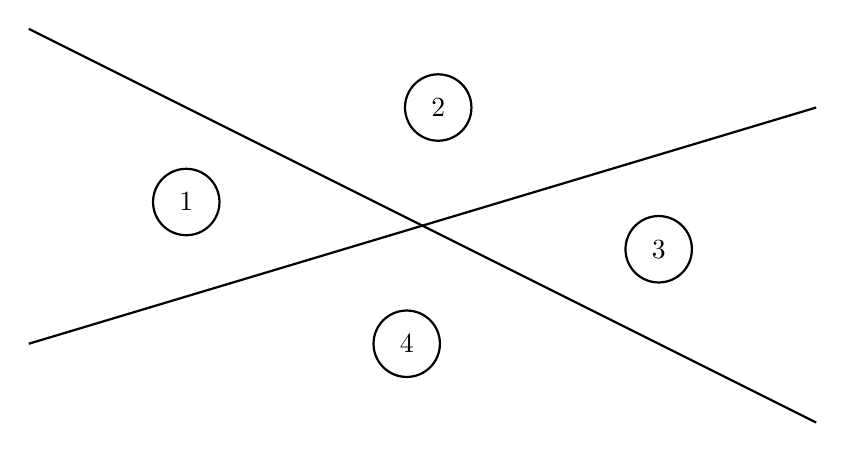
\begin{tikzpicture}[thick]
        \draw (-5,2.5) -- (5,-2.5);
        \draw (-5,-1.5) -- (5,1.5);
        \node[draw,circle,minimum size=24pt,inner sep=0,anchor=center] at (-0.2,-1.5) {$4$};
        \node[draw,circle,minimum size=24pt,inner sep=0,anchor=center] at (3,-0.3) {$3$};
        \node[draw,circle,minimum size=24pt,inner sep=0,anchor=center] at (-3,0.3) {$1$};
        \node[draw,circle,minimum size=24pt,inner sep=0,anchor=center] at (0.2,1.5) {$2$};
    \end{tikzpicture}
\end{center}

然而,这只是两条直线相交的一种\emph{具体情况}。我们怎么知道无论我们如何画这两条线,\emph{总能}得到四个区域?也就是说,我们能否以某种方式结合直线数量 $n = 2$ 这一事实来描述这是\text{如何}发生的?思考一下!

下面是我们的方法。请注意,当我们添加第二条直线时,每个已经存在的区域都会被分成两部分,并且\emph{无论你如何绘制直线},只要我们确保两条直线不平行,结果都是这样。也就是说,如果我们用一条直线将平面分成两个区域,

\begin{center}
    \begin{tikzpicture}[thick]
        \draw (-5,2.5) -- (5,-2.5);
        \node[draw,circle,minimum size=24pt,inner sep=0,anchor=center] at (-3,0.3) {$1$};
        \node[draw,circle,minimum size=24pt,inner sep=0,anchor=center] at (0.2,1.5) {$2$};
    \end{tikzpicture}
\end{center}

然后添加一条新的直线会将每个现有区域分成两部分。这会向整个平面添加两个新的区域,总共四个区域:

\begin{center}
    \begin{tikzpicture}[thick]
        \draw (-5,2.5) -- (5,-2.5);
        \draw [color=red] (-5,-1.5) -- (0,0)  node[midway,below,sloped]{分割区域 1}
        -- (5,1.5) node[midway,above,sloped]{分割区域 2} ;
        \node[draw,circle,minimum size=24pt,inner sep=0,anchor=center,color=red] at (-0.2,-1.5) {$4$};
        \node[draw,circle,minimum size=24pt,inner sep=0,anchor=center,color=red] at (3,-0.3) {$3$};
        \node[draw,circle,minimum size=24pt,inner sep=0,anchor=center] at (-3,0.3) {$1$};
        \node[draw,circle,minimum size=24pt,inner sep=0,anchor=center] at (0.2,1.5) {$2$};
    \end{tikzpicture}
\end{center}

当 $n = 3$ 时呢?在这种情况下,我们需要考虑向具有两条直线和四个区域的图形中添加第三条直线。我们想要提出一个不依赖于线的特定排列的论证,因此我们最终唯一能用的事实是线之间互不平行,且任何交点仅位于两条线(而不是三条或更多)上。不过,就目前而言,查看特定的线条排列会有所帮助,以便我们讨论相同的图形;我们可以利用对这个特定图形的观察来指导我们的一般论证。让我们从下方具有两条直线的图开始,向其中添加第三条线,我们让第三条线的交点都在初始交点``附近''或在图的范围内,这样我们就缩放图形了:

\begin{center}
    \begin{tikzpicture}[thick]
        \draw (-5,2.5) -- (5,-2.5);
        \draw (-5,-1.5) -- (5,1.5);
        \draw [color=red] (-5,1) -- (-1.8085,0.9043) node[midway,below,sloped]{\small 分割区域 1} 
        -- (2.5758,0.7727) node[midway,above,sloped]{\small 分割区域 2}
        -- (5,0.7) node[midway,below,sloped]{\small 分割区域 3};
        \node[draw,circle,minimum size=16pt,inner sep=0,anchor=center] at (-0.2,-1.5) {$4$};
        \node[draw,circle,minimum size=16pt,inner sep=0,anchor=center] at (3,-0.3) {$3$};
        \node[draw,circle,minimum size=16pt,inner sep=0,anchor=center] at (-3,-0.3) {$1$};
        \node[draw,circle,minimum size=16pt,inner sep=0,anchor=center] at (0.2,2) {$2$};
        \node[draw,circle,minimum size=16pt,inner sep=0,anchor=center,color=red] at (-4,1.45) {$5$};
        \node[draw,circle,minimum size=16pt,inner sep=0,anchor=center,color=red] at (0.1,0.45) {$6$};
        \node[draw,circle,minimum size=16pt,inner sep=0,anchor=center,color=red] at (4.61,1.05) {$7$};
    \end{tikzpicture}
\end{center}

很明显现在我们有 $7$ 个区域。我们将第三条线设置为不同的颜色,以便我们可以识别``新''区域出现的位置:一个区域(下方区域,区域 $4$)保持不变,但其他三个区域被一分为二,每个``分割''都会让我们的计数加 $1$(原来有 $1$ 个区域,现在有 $2$ 个)。如果我们以不同的方式绘制这条直线会怎样?

\begin{center}
    \begin{tikzpicture}[thick]
        \draw (-5,2.5) -- (5,-2.5);
        \draw (-5,-1.5) -- (5,1.5);
        \draw [color=red] (0,2.5) -- (-0.8333,0.4167) node[midway,right,sloped,rotate=-90]{\small 分割区域 2} 
        -- (-1.1364,-0.341) node[midway,left,sloped,rotate=-90]{\small 分割区域 1}
        -- (-2,-2.5) node[midway,right,sloped,rotate=-90]{\small 分割区域 4}; 
        \node[draw,circle,minimum size=16pt,inner sep=0,anchor=center] at (-0.2,-1) {$4$};
        \node[draw,circle,minimum size=16pt,inner sep=0,anchor=center] at (3,-0.3) {$3$};
        \node[draw,circle,minimum size=16pt,inner sep=0,anchor=center] at (-3,-0.3) {$1$};
        \node[draw,circle,minimum size=16pt,inner sep=0,anchor=center] at (1,2) {$2$};
        \node[draw,circle,minimum size=12pt,inner sep=0,anchor=center,color=red] at (-0.7,0.05) {$5$};
        \node[draw,circle,minimum size=16pt,inner sep=0,anchor=center,color=red] at (-1.5,1.8) {$6$};
        \node[draw,circle,minimum size=16pt,inner sep=0,anchor=center,color=red] at (-2.5,-1.4) {$7$};
    \end{tikzpicture}
\end{center}

同样的现象再次发生,其中一个区域保持不变,但其他三个区域一分为二。(我们怎么知道没有任何其他区域未绘制在我们这个比例的图形内?这并不像看上去的那么容易回答,值得深刻考虑。)尝试三条线的其他排列方式,并试图说服自己这种情况总会发生;此外,思考一下\emph{为什么}会出现这种情况,以及我们\emph{如何}解释这种情况一定会发生。不过,在给出一般性解释之前,我们先来看另一个小案例。

当 $n = 4$ 时,我们从 $3$ 条直线和 $7$ 个区域的平面开始,然后添加第四条直线,该线不与任何现有线平行,并且不穿过任何现有交点。同样,我们想要提出一个与特定的线条排列无关的论证,但是查看下面的具体图形将有助于引导我们的直觉来提出该论证:

\begin{center}
    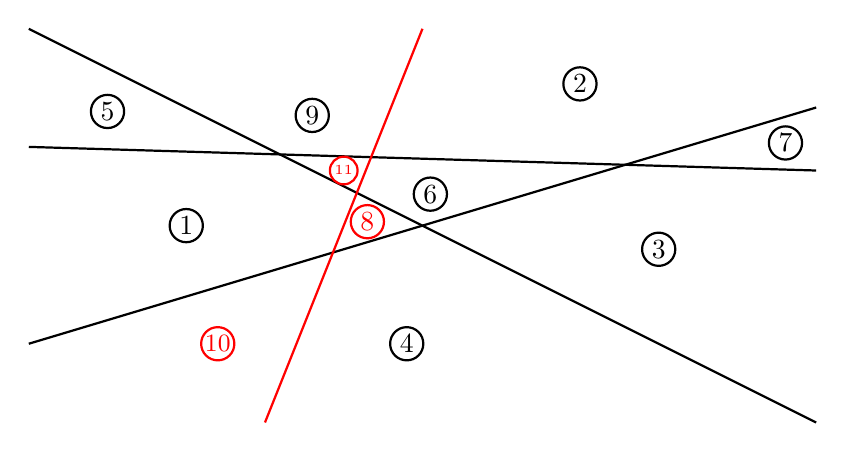
\begin{tikzpicture}[thick]
        \draw (-5,2.5) -- (5,-2.5);
        \draw (-5,-1.5) -- (5,1.5);
        \draw  (-5,1) -- (5,0.7);
        \draw [color=red] (0,2.5) -- (-2,-2.5);
        \node[draw,circle,minimum size=12pt,inner sep=0,anchor=center] at (-0.2,-1.5) {$4$};
        \node[draw,circle,minimum size=12pt,inner sep=0,anchor=center] at (3,-0.3) {$3$};
        \node[draw,circle,minimum size=12pt,inner sep=0,anchor=center] at (-3,0) {$1$};
        \node[draw,circle,minimum size=12pt,inner sep=0,anchor=center] at (2,1.8) {$2$};
        \node[draw,circle,minimum size=12pt,inner sep=0,anchor=center] at (-4,1.45) {$5$};
        \node[draw,circle,minimum size=12pt,inner sep=0,anchor=center] at (-1.4,1.4) {$9$};
        \node[draw,circle,minimum size=10pt,inner sep=0,anchor=center,color=red] at (-1,0.7) {\tiny $11$};
        \node[draw,circle,minimum size=12pt,inner sep=0,anchor=center] at (4.61,1.05) {$7$};
        \node[draw,circle,minimum size=12pt,inner sep=0,anchor=center,color=red] at (-0.7,0.05) {$8$};
        \node[draw,circle,minimum size=12pt,inner sep=0,anchor=center] at (0.1,0.4) {$6$};
        \node[draw,circle,minimum size=12pt,inner sep=0,anchor=center,color=red] at (-2.6,-1.5) {\small $10$};
    \end{tikzpicture}
\end{center}

请注意,三个原始区域保持不变(区域 $3$、区域 $5$ 和区域 $7$),其他四个区域一分为二。你注意到这里存在一个模式吗?似乎对于我们检查过的每个 $n$,添加第 $n$ 条线会使 $n-1$ 个区域保持不变,而其余区域则被一分为二。让我们尝试解释为什么会出现这种情况。请记住,当我们绘制 $n$ 条直线时,我们试图确定出现了多少个区域,因此让我们为该值分配一个``名称'',以便我们可以引用它;假设 $R(n)$ 表示在平面上绘制 $n$ 条直线所创建的区域数,且没有两条线平行,并且没有交点在两条以上的线上。在上面示例中,我们考虑了 $n$ 的较小取值,并研究了添加新的直线时会发生什么变化;也就是说,我们可以通过已知 $R(n - 1)$ 算出 $R(n)$ 的值。让我们整理一下我们的观察结果,以便它们适用于\emph{任意} $n$ 值。

假设我们已知 $R(n)$。(为什么我们可以这样做?对于某个特定的 $n$,我们是否确实知道 $R(n)$ 的特定值?这个值是什么?如何知道的?)假设我们在平面上有一个\emph{任意} $n$ 线图,满足上面题目陈述中给出的两个条件。这些直线创建了多少个区域?是的,正是 $R(n)$。现在,当我们添加第 $(n + 1)$ 条直线时会发生什么?关于这条线以及它如何改变图形,我们可以确定什么?其实,我们真正掌握的唯一信息是:

\begin{enumerate}[label=(\alph*)]
    \item 这条新的直线与现有的 $n$ 条直线中的任何一条都不平行;
    \item 这条新的直线不经过任何现有的交点。
\end{enumerate}

现在,条件 (a) 告诉我们这条新的直线必须与\emph{所有}现有的 $n$ 条直线线相交;平行线不相交,非平行线必然相交于某处。因此,我们必须在图上创建 $n$ 个新的交点。这些交点会与任何现有交点重合吗?不会!这正是条件 (b) 告诉我们的。这两条信息合在一起告诉我们,无论我们如何绘制这条新的直线,只要它满足题目的要求,这条直线上\emph{一定}会出现 $n$ 个``特殊''点。这些特殊点正是新线与现有线的交点。

我们现在想利用这些特殊点来识别图中的新区域。回顾一下我们上面研究的案例:识别新的交点,看看是否可以将它们与新的区域关联起来。也许用圆点标记这些交点并用 $\textbf{×}$ 标记新区域会有所帮助,让它们更容易辨认。我们在下面为你展示了一个示例,其中 $n = 4$。你注意到了什么?你能用这些点来帮助识别添加第 $n$ 条直线后创建了多少新区域吗?思考一下,然后继续阅读。

\begin{center}
    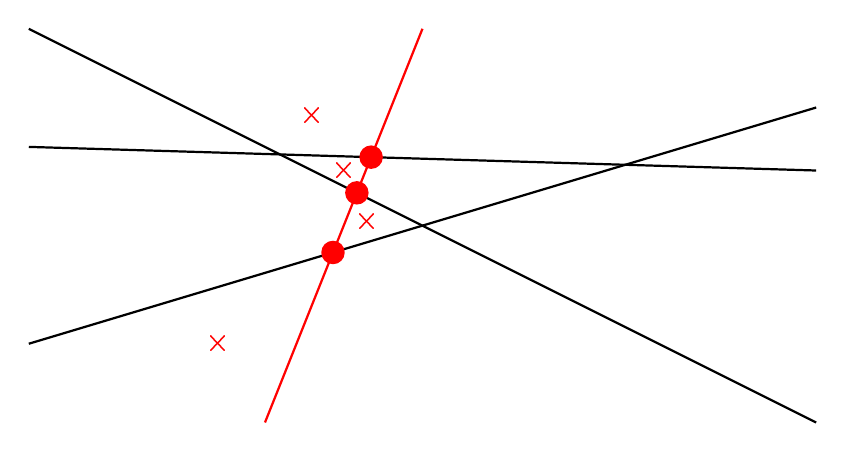
\begin{tikzpicture}[thick]
        \draw (-5,2.5) -- (5,-2.5);
        \draw (-5,-1.5) -- (5,1.5);
        \draw  (-5,1) -- (5,0.7);
        \draw [color=red] (0,2.5) -- (-2,-2.5);
        \node[minimum size=14pt,anchor=center,color=red,very thick] at (-1.4,1.4) {$\textbf{×}$};
        \node[minimum size=14pt,anchor=center,color=red,very thick] at (-1,0.7) {$\textbf{×}$};
        \node[minimum size=14pt,anchor=center,color=red,very thick] at (-0.7,0.05) {$\textbf{×}$};
        \node[minimum size=14pt,anchor=center,color=red,very thick] at (-2.6,-1.5) {$\textbf{×}$};
        \node[fill,circle,inner sep=3pt,color=red] at (-0.6522,0.8696) {};
        \node[fill,circle,inner sep=3pt,color=red] at (-0.8333,0.4167) {};
        \node[fill,circle,inner sep=3pt,color=red] at (-1.1364,-0.341) {};
    \end{tikzpicture}
\end{center}

没错!任意两个相邻新交点之间,都有一条\emph{线段}将一个区域一分为二!剩下的就是确定我们创建了多少个新的此类线段。由于每条线段都将唯一\emph{一个}现有区域一分为二,因此这将准确地告诉我们创建了多少个新区域。我们已知,第 $(n + 1)$ 条直线线创建了 $n$ 个新的交点。想想这些点是如何排列在直线上的。任意两个``连续''点都会创建一条线段,但极点也会创建无限线段(永远延申下去经过这些极点)。总共有多少个?正好是 $n + 1$。(参考上图,$n = 3$。我们看到有 $3$ 个新交点和 $4$ 条新线段,其中两个是无限射线。)这意味着有 $n + 1$ 条线段将区域一分为二,因此我们恰好创建了 $n + 1$ 个新区域!这让我们可以说
\[R(n + 1) = R(n) + n + 1\]
哇,多好的观察啊!我们花了一些时间研究示例并进行了一些几何论证,但最终我们做到了。我们已经确定了这个问题的一些归纳结构;我们发现一个情况如何依赖另一个情况。也就是说,我们发现了 $R(n+1)$ 如何依赖 $R(n)$。这还没有完全解决这个问题,但我们现在已经非常接近了。剩下的就是用类似的表达式替换 $R(n)$,并不断执行此操作,直到达到我们已知的 $R(1) = 2$。观察:

\begin{center}
    \begin{tabular}{rcccccccccc}
        $R(n+1)$ & $=$ &          & &            &     &            &     & $\cancel{R(n-1)}$ & $+$ & $n+1$\\
                 & $=$ &          & &                   &     & $\cancel{R(n-1)}$ & $+$ & $n$ & $+$ & $n+1$\\
                 & $=$ &          & & $\cancel{R(n-2)}$ & $+$ & $(n-1)$           & $+$ & $n$ & $+$ & $n+1$\\
                 & $\vdots$ &     & &  &  &  &  &  &  & \\
                 & $=$ &          & & $\cancel{R(2)}+3$ & $+$ & $\dots$ & $+$ & $n$ & $+$ & $n+1$ \\
                 & $=$ & $R(1)+2$ & $+$ & $3$               & $+$ & $\dots$ & $+$ & $n$ & $+$ & $n+1$ \\
    \end{tabular}
\end{center}

因为我们知道 $R(1) = 2$,所以我们可以说
\[R(n + 1) = 2 + \big(2 + 3 + \dots + n + (n + 1)\big) = 2 + \Bigg(\sum_{k=1}^{n+1}k\Bigg)-1 = 1+\sum_{k=1}^{n+1}k\]
而这正是我们之前研究过的求和公式!(另请注意,我们必须减去 $1$,因为括号中缺少求和的第一项。)回想一下 $\sum_{k=1}^{n} k = \frac{n(n+1)}{2}$,为了表示上面等式中的求和,我们只需将 $n$ 替换为 $n + 1$ 即可。因此,
\[R(n + 1) = 1+\frac{(n+1)(n+2)}{2}\]
我们要进行的最后一步简化是将整个方程中的 $n+1$ 替换为 $n$,因为使用 $R(n)$ 的表达式更有意义(对 $n$ 的值有什么要求?)
\[R(n + 1) = 1+\frac{n(n+1)}{2}\]
最终,我们找到了开头问题的答案!在这个过程中,我们采用了\emph{归纳}技术:我们解释了一个``事实''(即 $R(n + 1)$ 的值)如何\emph{取决于}``前一个事实''(即 $R(n)$ 的值),并使用这些迭代依赖关系进行反向运算,直到达到一个特定的\emph{已知}值,即 $R(1)$。

我们想再次指出,我们在本节中所做的推导和观察只是引导我们的直觉从而得出答案,并不是\emph{严格证明}。问题出在 ``$\dots$'' 身上,省略号不是具体的、``官方''的数学方法来捕获归纳技术背后的归纳过程。此外,我们解决``平面中的线''问题的方法是从 $n - 1$ 条线的图形\emph{开始,构建}一个包含 $n$ 条线的新图;这样可以吗?为什么这实际上告诉了我们有关 $n$ 条线的\emph{任意}图的信息?所有这些图都来自于少了一条线的较小图吗?

在接下来的两章中,我们将学习必要的工具来充分描述我们迄今为止所做事情的严格方法,在那之后的章节中,我们将使用这些工具让数学归纳法变得正式而严谨。不过,现在我们想给出归纳法的启发式定义,并继续研究依赖归纳技术的有趣问题和观察结果。练习这些类型的问题 --- 学习何时识别归纳过程、如何使用它、如何使用该结构来解决问题等等 --- 将在未来非常有帮助,我们不需要深入到数学技术细节。(至少,现在还不需要!)


% !TeX root = ../../../book.tex
\subsection{习题}

\subsubsection*{温故知新}

以口头或书面的形式简要回答以下问题。这些问题全都基于你刚刚阅读的内容,所以如果忘记了具体的定义、概念或示例,可以回去重读相关部分。确保在继续学习之前能够自信地回答这些问题,这将有助于你的理解和记忆!

\begin{enumerate}[label=(\arabic*)]
    \item 归纳过程有哪些特征?
    \item 我们如何证明 $\sum_{k=1}^{n}k = \frac{n(n+1)}{2}$ 是正确的?我们的方法是如何归纳的?(如果你不记得了,请重读第 \ref{sec:section1.4.2} 节!)
    \item 为什么我们可以把上一个问题中提到的求和公式,用 $n+1$ ``替换'' $n$,并且知道它仍然成立?我们也可以将 $n$ 替换为 $n - 1$ 吗?
    \item 通过代数步骤获得前 $n$ 个自然数平方和的最终表达式;也就是说,验证
    \[\frac{1}{3}(n+1)^3-\frac{1}{3}(n+1)-\frac{n(n+1)}{2} = \frac{1}{6}n(n+1)(2n+1)\]
    \item 试着回忆一下向平面中添加第 $(n+1)$ 条直线正好会创建 $n+1$ 个新区域的论点。你能为朋友证明这个论点并说服他/她它是有效的吗?
    \item 求前 $n$ 个自然数的平方和,为什么不能把前 $n$ 个自然数之和的公式平方呢?为什么这是错误的?
\end{enumerate}

\subsubsection*{小试牛刀}

尝试回答以下问题。这些题目要求你实际动笔写下答案,或(对朋友/同学)口头陈述答案。目的是帮助你练习使用新的概念、定义和符号。题目都比较简单,确保能够解决这些问题将对你大有帮助!

\begin{enumerate}[label=(\arabic*)]
    \item 在平面中画 $5$ 条直线(满足原题的两个条件)并验证是否有 $16$ 个区域。你还能验证 $6$ 条线产生 $22$ 个区域吗?
    \item 给出序列 $1, 2, 3, 4, \dots , 100$ 的另一种解释,而不仅仅是从 $1$ 到 $100$ 的所有自然数。(回想一下我们给出的例子:$1$ 到 $100$ 之间所有英文拼写中不含字母``i''的数字。)
    \item 提出一个将 $(n + 1)^4$ 与 $n^4$ 联系起来的代数表达式,就像我们对立方所做的那样。\\ 
    (\textbf{挑战题:}你能为刚刚推导出的表达式给出\emph{几何}解释吗?)
    \item \textbf{挑战题:}让我们将``平面上的线''这题提升一个维度!考虑三维空间中有 $n$ 个平面。会创建多少个区域?假设没有两个平面平行,并且没有三个或以上平面相交于一条直线。(想想这两个条件如何直接类比于``线''那题的给定条件。)
\end{enumerate}

\newpage
% !TeX root = ../../../book.tex
\section{定义归纳}

为了阐明数学归纳法这一证明技术,我们需指出:前一节的示例依赖于问题结构的直观理解来给出``解''——此处\emph{解}上加引号表明尚未严格证明。由此引出核心问题:若我们被要求直接验证先前推导的公式,而未曾通过直观过程获得它,仅被告知其正确性,该如何证明?这正是当前面临的情形,除非告知者采用了与我们相同的直观论证。

假设一位持怀疑态度的朋友声称:``我听说计算前 $n$ 个自然数平方和的公式是 $\frac{1}{6}n(n+1)(2n+1)$。验证前两个数完全吻合,因此它必然正确,可以确信无疑!''作为理性的思考者兼好友,你回应道:``我也听闻此公式,但需确保它对所有自然数均成立。''如何展开验证?朋友所言非虚,前几项确实``完美匹配'':
\begin{align*}
    1^2 &= \enspace 1 = \frac{1}{6}(1)(2)(3) \\
    1^2 + 2^2 &= \enspace 5 = \frac{1}{6}(2)(3)(5) \\
    1^2 + 2^2 + 3^2 &= 14 = \frac{1}{6}(3)(4)(7) \\
    1^2 + 2^2 + 3^2 + 4^2 &= 30 = \frac{1}{6}(4)(5)(9)
\end{align*}
如果我们愿意的话,甚至可以手动检验更大的 $n$ 值:
\[1^2 + 2^2 + 3^2 + 4^2 + 5^2 + 6^2 + 7^2 + 8^2 + 9^2 + 10^2 = 385 = \frac{1}{6}(10)(11)(21)\]
然而该公式宣称对\emph{任意} $n$ 成立。自然数有\emph{无穷}多个,逐一验证从数学和时间上皆不可行——无论检验多少独立的 $n$ 值,总会有更大的 $n$ 值未经验证。我们如何\emph{确知}公式不会在某个较大的 $n$ 值失效?这要求一种数学上\emph{高效}的方法,能以有限步骤验证所有情形。为此我们引入初步构想(后续将严格表述的数学归纳法),从原理层面说明其运作机制。

% !TeX root = ../../../book.tex
\subsection{多米诺骨牌类比}

假设我们有一副特殊的多米诺骨牌,它包含无穷多张骨牌!每张骨牌可以书写任意内容,而非标准的点数。这些骨牌沿无限延伸的桌面排列成无限长的一行。从侧面观察时,每张骨牌下方标有位置标签:

\begin{center}
    \begin{tikzpicture}
        \foreach \x in {1,...,5}
        {
            \pic [fill=white] at (\x, 0, 0) {annotated cuboid={width=3, height=30, depth=10}};
            \node[below] at (\x, -3){\tiny $n=\x$};
        }
        \node[anchor=center] at (6.5, -1.5){\LARGE $\dots \cdot$};
        % \pic [very thick,densely dashed,draw=blue] at (5,0) {annotated cuboid={width=30, height=5, depth=10, opacity=0.2}};
    \end{tikzpicture}
\end{center}

对于这个特定的例子,我们需要验证公式
\[\sum_{k=1}^{n}k^2 = \frac{1}{6}n(n+1)(2n+1)\]
为此,设想每张多米诺骨牌记载一个特定``事实''。具体来说,我们可以想象第一张多米诺骨牌上写有表达式
\[\sum_{k=1}^{1}k^2 = \frac{1}{6}(1)(1)(3)\]
第二张多米诺骨牌上写有表达式
\[\sum_{k=1}^{2}k^2 = \frac{1}{6}(2)(3)(5)\]
推而广之,第 $n$ 张骨牌写有如下``事实'':
\[\sum_{k=1}^{n}k^2 = \frac{1}{6}n(n+1)(2n+1)\]
由于多米诺骨牌具有连锁倾倒的特性,我们约定骨牌倒下即表示其记载的``事实''是\emph{真实命题}。由此将多米诺骨牌的物理解释与公式有效性的数学解释联系起来。

我们已手动验证 $n=1$ 的情形:$1^2=\frac{1}{6}(1)(2)(3)$,故第一张骨牌记载的命题为真,必将倒下。同理验证 $n=2$ 后,第二张骨牌也会倒下:

\begin{center}
    \begin{tikzpicture}
        \foreach \x in {1,2}
        {
            \pic [fill=white, rotate=-30, anchor=south] at (\x, -0.15, 0) {annotated cuboid={width=3, height=32, depth=10}};
            \node[below] at (\x-1.5, -3){\tiny $n=\x$};
        }
        \foreach \x in {3,4,5}
        {
            \pic [fill=white] at (\x, 0, 0) {annotated cuboid={width=3, height=30, depth=10}};
            \node[below] at (\x, -3){\tiny $n=\x$};
        }
        \node[anchor=center] at (6.5, -1.5){\LARGE $\dots \cdot$};
        % \pic [very thick,densely dashed,draw=blue] at (5,0) {annotated cuboid={width=30, height=5, depth=10, opacity=0.2}};
    \end{tikzpicture}
\end{center}
然而,若继续逐个检验,又会陷入原先的困境——我们不可能验证\emph{每张}骨牌。真正的需求是捕捉多米诺效应的精髓:一张骨牌倒下将触发下一张倒下。这要求我们建立相邻骨牌所载``事实''的数学关联。

让我们看看前两张多米诺骨牌的情况。既然知道骨牌 $1$ 倒下,我们能否在不重写所有求和项的情况下确保骨牌 $2$ 倒下?两块骨牌上的陈述有何关联?每个陈述都是自然数的平方和,且第二张骨牌的陈述正好多出一项。因此,利用骨牌 $1$ 上已知的\emph{真实陈述},可以\emph{验证}骨牌 $2$ 上陈述的真实性:
\[\sum_{k=1}^{2}k^2 = 1^2+2^2=1+2^2=5=\frac{1}{6}(2)(3)(5)\]
尽管节省的唯一``工作''只是免于计算 $1^2=1$,但让我们在更大数字上应用此过程以凸显其优势。\emph{假设}骨牌 $10$ 已经倒下(其求和的完整验证已在前文给出),这意味着我们\emph{知道}
\[\sum_{k=1}^{10}k^2 =\frac{1}{6}(10)(11)(21)=285\]
是一个\emph{真实陈述}。利用它来验证骨牌 $11$ 的陈述:
\[\sum_{k=1}^{11}k^2 =\frac{1}{6}(11)(12)(23)\]
骨牌 $11$ 上的求和公式有 $11$ 项,前 $10$ 项正是骨牌 $10$ 上的求和!因此只需分离第 $11$ 项并代入已知结果:
\begin{align*}
    \sum_{k=1}^{11}k^2 &= (1^2+2^2+\dots+10^2)+11^2\\
    &=\sum_{k=1}^{10}k^2+11^2\\
    &=385+121\\
    &=506\\
    &=\frac{1}{6}3036=\frac{1}{6}(11)(12)(23)
\end{align*}
节省的工作量显而易见!既然已知前 $10$ 项之和,何必重新计算?

现在设想对\emph{所有} $n$ 值\emph{同时}实施此过程!若能证明每当骨牌 $n$ 倒下,骨牌 $(n + 1)$ \emph{必然}倒下,这意味着什么?回顾无穷骨牌序列:已知骨牌 $1$ 因手动检验而倒下,加之``骨牌 $n$ 撞倒骨牌 $(n + 1)$''的普适性验证,可推得骨牌 $1$ 撞倒骨牌 $2$,骨牌 $2$ 撞倒骨牌 $3$,骨牌 $3$ 撞倒骨牌 $4$,…… 如此传递下去,整列骨牌终将全部倒下!本质上,整个过程可归结为\emph{两步}:

\begin{enumerate}[label=(\arabic*)]
    \item 确保第一张骨牌倒下;
    \item 确保每张骨牌都能撞倒下一张骨牌。
\end{enumerate}
仅凭这两步,便能\emph{保证}所有骨牌倒下,从而\emph{证明}每个公式对\emph{任意}自然数 $n$ 成立。

我们已经完成步骤 (a),现在需要完成步骤 (b)。此前已针对特定案例(骨牌 $1$ 撞倒骨牌 $2$、骨牌 $10$ 撞倒骨牌 $11$)执行了此操作,现在将其推广到任意 $n$ 值。我们\emph{假设}:对于某个\emph{特定}但\emph{任意}的 $n$,多米诺骨牌 $n$ 会倒下,这意味着方程
\[\sum_{k=1}^{n}k^2=\frac{1}{6}n(n+1)(2n+1)\]
为\emph{真实陈述}。现在需将其关联到骨牌 $(n+1)$ 的陈述,并应用上述等式信息。将 $n+1$ 项的和拆分为 $n$ 项和与末项:
\[\sum_{k=1}^{n+1}k^2 = (1^2+2^2+\dots+n^2+(n+1)^2)=\sum_{k=1}^{n}k^2+(n+1)^2\]
根据骨牌 $n$ 倒下的假设(即其命题为真),可得
\[\sum_{k=1}^{n+1}k^2 = \frac{1}{6}n(n+1)(2n+1)+(n+1)^2\]
这与骨牌 $(n+1)$ 的命题是否一致?骨牌 $(n+1)$ 的``事实''与骨牌 $n$ 类似,只是将``$n$''替换为``$n + 1$'':
\[\sum_{k=1}^{n+1}k^2 = \frac{1}{6}\big(n+1\big)\big((n+1)+1\big)\big((2(n+1)+1)\big)=\frac{1}{6}(n+1)(n+1)(2n+3)\]
目前还不清楚我们推导出的表达式是否实际上等于上面的式子。我们可以尝试化简该表达式,并将其分解为与上面表达式``类似''的新表达式,但展开两个表达式并比较所有项可能会更容易。(这基于这样的一般思想:展开因式分解后的多项式比进行因式分解要容易得多。)对于第一个表达式,我们有
\begin{align*}
    \frac{1}{6}n(n + 1)(2n + 1) + (n + 1)^2 &=\frac{1}{6}n(2n^2 + 3n + 1) + (n^2 + 2n + 1)\\
    &= \frac{1}{3}n^3 + \frac{1}{2}n^2 + \frac{1}{6}n + n^2 + 2n + 1 \\
    &= \frac{1}{3}n^3 + \frac{3}{2}n^2 + \frac{13}{6}n + 1
\end{align*}
对于第二个表达式,我们有
\begin{align*}
    \frac{1}{6}(n+1)(n + 2)(2n + 3) &=\frac{1}{6}(n+1)(2n^2 + 7n+6)\\
    &= \frac{1}{6}\big[(2n^3 + 7n^2 + 6n) + (2n^2 + 7n + 6)\big] \\
    &= \frac{1}{3}n^3 + \frac{3}{2}n^2 + \frac{13}{6}n + 1
\end{align*}
可见两式相等!此外,请注意,这比尝试整理其中一个表达式并将其``变形''为另一个表达式要容易得多。我们通过展开两式并最终得到相同的表达来证明它们是相同的。现在,让我们回顾并总结我们所取得的成果:
\begin{enumerate}
    \item 我们将证明公式
    \[\sum_{k=1}^{n+1}k^2 = \frac{1}{6}n(n+1)(2n+1)+(n+1)^2\]
    对于\emph{所有} $n$ 值成立类比为推倒无穷多的多米诺骨牌。
    \item 通过手工计算验证骨牌 $1$ 的命题成立,骨牌 $1$ 倒下;
    \item \emph{假设}骨牌 $n$ 的命题为真,由骨牌 $n$ 命题成立推出骨牌 $(n+1)$ 命题成立,从而证明骨牌 $n$ 会撞倒骨牌 $(n+1)$。
    \item 由此保证所有骨牌都会倒下,因此公式对\emph{所有} $n$ 都成立。
\end{enumerate}
此方法是否严谨?是否已\emph{严格证明}公式对所有自然数 $n$ 都成立?若存在 $n$ 使得公式失效,这对多米诺骨牌体系意味着什么?

请记住,这里的多米诺骨牌类比只是理解归纳法工作原理的一个直观指引,并非建立在严格的数学基础之上。建立严格的数学基础将是接下来几章的目标。现在,让我们回顾本章讨论的另一个例子:直线划分平面区域。同样,在推导公式 $R(n)$ 时使用省略号显得繁琐,我们希望避免这种做法。让我们尝试将多米诺骨牌类比应用于此问题。

设想我们定义 $R(n)$ 为 $n$ 条直线在平面上划分出的不同区域的数量,这些直线满足互不平行且任意三条(或更多)直线不共点。进一步设想,我们在代表第 $n$ 步的骨牌上写下``$R(n) = 1 + \frac{n(n+1)}{2}$''这一``事实''。能否按照与之前相同的逻辑来验证所有骨牌都会倒下?

首先,需要验证骨牌 $1$ 是否会倒下。这等同于验证命题``$R(1) = 1+\frac{1(2)}{2} = 1+1 = 2$''是否成立。这显然成立,正如我们之前验证过的:一条直线将平面划分为两个区域。其次,需要证明对于\emph{任意} $n$,第 $n$ 块骨牌倒下必定导致第 $(n + 1)$ 块骨牌倒下。也就是说,我们\emph{假设}``$R(n) = 1 + \frac{n(n+1)}{2}$''对某个特定的 $n$ 成立,然后\emph{证明}``$R(n + 1) = 1 + \frac{(n+1)(n +2)}{2}$''也必然成立。如何证明?沿用之前的思路,建立 $R(n + 1)$ 与 $R(n)$ 的关系。向\emph{任意}满足条件的 $n$ 条直线的图形中添加一条新直线,通过几何分析,我们得到关系式 $R(n+1) = R(n) + n + 1$。利用此关系以及第 $n$ 块骨牌倒下的假设,可得:
\[R(n + 1) = R(n) + n + 1 = 1 +\frac{n(n+1)}{2}+ n + 1\]
这个结果是否与骨牌 $(n + 1)$ 上的表达式一致?通过化简比较即可验证:
\[1 +\frac{n(n+1)}{2}+ n + 1=2+n+\frac{n^2+n}{2} = \frac{1}{2}n^2+\frac{3}{2}n+2\]
以及
\[1 + \frac{(n+1)(n +2)}{2} = 1+\frac{n^2+3n+2}{2} =  \frac{1}{2}n^2+\frac{3}{2}n+2\]
结果完全相同!因此,我们证明了对于\emph{任意} $n$,骨牌 $n$ 倒下\emph{必然}导致骨牌 $(n+1)$ 倒下。

思考一下,使用这种``多米诺骨牌技术''进行的证明,与我们之前为推导该公式所采用的方法有何不同?我们在本节中是否使用了省略号?为何这种证明方式更优?我们是否曾用多米诺骨牌归纳技术来推导公式本身?


% !TeX root = ../../../book.tex
\subsection{其他类比}

多米诺骨牌类比非常流行,但它并非描述归纳法工作方式的唯一途径。根据阅读材料或交流对象的不同,你可能会接触到不同的类比或其他形式的阐释。在此,我们将介绍两种常见的类比。思考这些类比在本质上的相通之处,将有助于深化你对归纳法的理解(至少基于我们已有的探讨)。

\subsubsection*{神奇的数学猴子 Mojo}

想象一架直冲云霄的无穷天梯,梯级按 $1, 2, 3$ 的顺序无限延伸。我们的朋友 Mojo 伫立在梯子旁。这只聪慧的猴子痴迷数学,更拥有神奇的能力——他能真正攀爬这架无穷天梯!

Mojo 踏上某一级阶梯,即代表与该数字对应的事实成立。如何确保他爬完整架梯子?逐一检查每级阶梯效率低下:我们需要先确认他抵达第 $1$ 级,再验证他到达第 $2$ 级,接着是第 $3$ 级……如此往复。更高效的方法是在 Mojo 攀爬前确认两点:第一,他是否踏上起点(即第 $1$ 级)?若是,那就太好了!第二,阶梯间距是否足够近,使他无论身处何处,\emph{总能}登上下一级?若满足此条件,那就更棒了!这些要求与多米诺骨牌类比中的条件完全一致。要确保 Mojo 抵达\emph{每一级}阶梯,只需确认他踏上第 $1$ 级并能持续迈向下一级。

\subsubsection*{归纳鸭 Doug}

再来认识一下 Doug ——一只酷爱面包的鸭子。为了觅食,他会造访数学镇归纳街上每户人家的院子。这些院子沿街排列,门牌号依次为 $1, 2, 3, \dots$。

Doug 从 $1$ 号院子开始搜寻面包。一无所获的他饥肠辘辘,便转向隔壁的 $2$ 号院子。再次空手而归的他只能继续前行。此时已知 $1$ 号院无面包,因此唯一的选择只能是隔壁的 $3$ 号院……我想你已预见到了结局。

如果我们追踪 Doug 的行迹,我们或许好奇他是否终将踏足每个院子。假设已知\emph{所有院子均无面包},这意味着每当 Doug 身处某院,必将前往隔壁院子继续寻找。由此,他必定会挨家挨户探索!换言之,无论你住在编号多大的房子,终将在某一刻目睹 Doug 在你的后院徘徊(遗憾的是,他永远腹中空空——可怜的 Doug!)。


% !TeX root = ../../../book.tex
\subsection{总结}

回顾前两个示例的工作及我们的类比,可以发现每个问题都具有特定的\emph{结构}:某个``事实''依赖于``前一个事实''。对于立方数,我们找到了用 $n^3$ 表示 $(n + 1)^3$ 的方法;对于平面分割问题,我们刻画了向 $n$ 条直线的图形添加新直线时新增的区域个数。基于这些观察,我们反复应用已知关系,直至抵达一个可验证的``基础事实''——通常对应较小的 $n$ 值(两例中均为 $n = 1$)。这一过程使我们能够推导出适用于\emph{任意} $n$ 的通用公式或表达式。

尽管这项工作对公式推导至关重要且富有启发性,但它本身\emph{不足以证明}公式的有效性。在进行上述工作时,我们发现了归纳过程的存在,并利用其结构推导了相关表达式。这实际上有两个好处:不仅发现了待证公式,还让我们意识到采用\emph{数学归纳法}进行严格证明的可行性。

实际的``归纳证明''包含两个核心步骤:首先,验证公式在某个``起始值''成立;其次,\emph{假设}公式对某个特定 $n$ 成立,并以此证明其对 $n + 1$ 必然成立。完成这两步后,我们即可断言``所有多米诺骨牌都会倒下''——公式对所有相关 $n$ 值都成立。

\subsubsection*{一个问题:梯子的``尽头''是什么?}

你可能仍存疑虑,我们尝试在此预测你的担忧。(之所以提及这一点,是因为这是一个常见疑问。若你\emph{未曾}考虑这一点,请试着想象其来源。)你或许会说:``等等,现在我明白 Mojo 如何攀登天梯了,但他如何真正\emph{抵达顶端}呢?这是个无穷阶梯,对吗?那他永远无法到达终点……不是吗?''

某种意义上,你是对的。既然这个神奇阶梯将\emph{永远}延伸,它便没有真正的终点,Mojo 永无法抵达``顶端''。然而,这并非关键;我们不在意任何``\emph{顶端}''(不仅仅是因为\emph{不存在}顶端),只需确认 Mojo 能踏足\emph{每一个}台阶。他不必凌驾所有台阶立于顶端俯视来路——那不是目的!知道 Mojo 实际上到达了\emph{每一个可能的}阶梯。他不必超越所有人,站在梯子的顶端,俯视自己的来路。那不是目标!

不妨这样思考:假设你对某个待证事实抱有浓厚兴趣,例如
\[\text{事实\ } \#18,458,789,572,311,000,574,003 \text{\ (具体数值无关紧要)}\]
它对应遥不可及的台阶,而你只关心 Mojo 能否抵达。他会到达吗?他当然会!这或许需要漫长的时光(多少步呢?),但这在猴子与梯子的神奇世界,谁又在乎时间呢?你知道他终将抵达,这就够了。试想每个事实在神奇世界里都有专属关注者,每位关注着都将因 Mojo 踏足其关切之阶而欣喜。无人在意他能否登顶——那并非焦点。与此同时,在现实世界中,我们因\emph{所有}关注者终将如愿而欣慰。无限攀登的过程被简化为两步:仅凭此两步,我们便确信阶梯的\emph{每一级}皆可达,每个编号的事实皆成立。

亦可类比多米诺骨牌:我们是否在意骨牌链存在``终点'',最终撞上墙壁?当然不。骨牌链将永续延伸,每张牌终会倒下,时间长短无关紧要。同理,我们知晓 Doug 终将抵达\emph{所有}院子——何时抵达\emph{某个}院子无关紧要,唯有抵达\emph{全部}院子方为关键。


% !TeX root = ../../../book.tex
\subsection{习题}\label{sec:section2.3.4}

\subsubsection*{温故知新}

以口头或书面的形式简要回答以下问题。这些问题全都基于你刚刚阅读的内容,所以如果忘记了具体的定义、概念或示例,可以回去重读相关部分。确保在继续学习之前能够自信地回答这些问题,这将有助于你的理解和记忆!

\begin{enumerate}[label=(\arabic*)]
    \item 多米诺骨牌、Mojo 和 Doug 类比是如何等价的?你能给出``函数''来描述它们的关系,将一种类比转换成另一种类比吗?
    \item 找一个没学过数学归纳法的朋友,试着向他描述一下数学归纳法。你发现自己使用了其中的类比吗?有帮助吗?
    \item 为什么我们对立方体的研究未能证明求和公式?为什么我们还需要完成所有这些工作?
    \item 想想多米诺骨牌的类比。多米诺骨牌永远持续下去是一个问题吗?这是否意味着有些多米诺骨牌永远不会倒下?尝试用类比来描述这意味着什么。
\end{enumerate}

\subsubsection*{小试牛刀}

尝试回答以下问题。这些题目要求你实际动笔写下答案,或(对朋友/同学)口头陈述答案。目的是帮助你练习使用新的概念、定义和符号。题目都比较简单,确保能够解决这些问题将对你大有帮助!

\begin{enumerate}[label=(\arabic*)]
    \item 通过归纳步骤来证明该公式
    \[\sum_{k=1}^{n}k = \frac{n(n+1)}{2}\]
    \item 通过归纳步骤来证明该公式
    \[\sum_{k=1}^{n}2k-1 = n^2\]
    \item 通过归纳步骤来证明该公式
    \[\sum_{k=1}^{n}k^3 = \Bigg(\frac{n(n+1)}{2}\Bigg)^2\]
    \item 假设我们有一系列由自然数索引的事实。我们使用表达式 ``$P(n)$'' 表示第 $n$ 个事实。
    \begin{enumerate}[label=(\alph*)]
        \item 如果我们想证明对于每个自然数 $n$,\emph{每个}事实都为真,我们应该怎么做呢?
        \item 如果我们想证明只有 $n$ 为\emph{偶数}时对应的陈述才为真,那该怎么办?我们能做到吗?你能用我们给出的一个类比稍作修改来描述你的方法吗?
        \item 如果我们想证明只有 $n$ 大于等于 $4$ 时才对应的陈述才为真,那该怎么办?我们能做到吗?你能用我们给出的一个类比稍作修改来描述你的方法吗?
    \end{enumerate}
\end{enumerate}


\newpage
% !TeX root = ../../../book.tex
\section{另外两个(不同的)例子} \label{sec:section2.4}

本节有两个主要目的。首先,我们旨在避免读者产生归纳法仅适用于证明\emph{数值公式}(如涉及数字或多项式)的误解。归纳法的应用远比这广泛得多!特别是接下来的例子将证明:某些抽象性质对于给定情境中的任意``规模''均成立。我们会看到这仍属于``归纳''的范畴,同时也能观察到其与先前例子的区别。此外,这些例子还揭示了一个重要现象:有时推动多米诺骨牌需要掌握``更多信息''。在之前的案例中,仅需确认骨牌 $n$ 倒下,即可\emph{确保}骨牌 $n + 1$ 随之倒下。但在本节的示例中,我们可能需要了解前几个骨牌的状态。通过这两个例子,我们将总结其与前述多米诺骨牌模型的差异,并预览适用于此类情况的、更通用的归纳技术定义。

% !TeX root = ../../../book.tex
\subsection{多米诺与密铺} \label{sec:section2.4.1}

这个示例比前两个稍显复杂。我们最终仍将证明某个数值公式,但问题本身比单纯操纵代数表达式更直观。此外,在开始阶段我们会注意到一个有趣的现象:必须先解决几个``小案例'',才能推广方法。这将是我们首次探讨如何调整归纳技术以适应其他情况。

我们要回答的问题可以表述如下:

\begin{quote}
    给定一个由 $2 \times n$ 个方格组成的棋盘,有多少种不同的方式能用多米诺骨牌完全覆盖(密铺)该棋盘?覆盖时每个方格必须被有且仅有一块多米诺骨牌覆盖。
\end{quote}
例如,以下是正确的密铺:

\begin{center}
    
\begin{tikzpicture}[x=1.0cm, y=1.0cm]
        \foreach \y in {0,1} {
            \foreach \x in {0,...,3} {
                \draw (0+\x ,0+\y) rectangle ++ (1,1);
            }
        }

        \draw[fill, black] (0.25 ,0.25) rectangle ++ (1.5,0.5);
        \draw[fill, black] (0.25 ,1.25) rectangle ++ (1.5,0.5);
        \draw[fill, black] (2.25 ,0.25) rectangle ++ (0.5,1.5);
        \draw[fill, black] (3.25 ,0.25) rectangle ++ (0.5,1.5);

        \foreach \y in {0,1} {
            \foreach \x in {0,...,3} {
                \draw (5+\x ,0+\y) rectangle ++ (1,1);
            }
        }

        \draw[fill, black] (5+1.25 ,0.25) rectangle ++ (1.5,0.5);
        \draw[fill, black] (5+1.25 ,1.25) rectangle ++ (1.5,0.5);
        \draw[fill, black] (5+0.25 ,0.25) rectangle ++ (0.5,1.5);
        \draw[fill, black] (5+3.25 ,0.25) rectangle ++ (0.5,1.5);
    \end{tikzpicture}
\end{center}
而以下\emph{不}是正确的密铺:

\begin{center}
    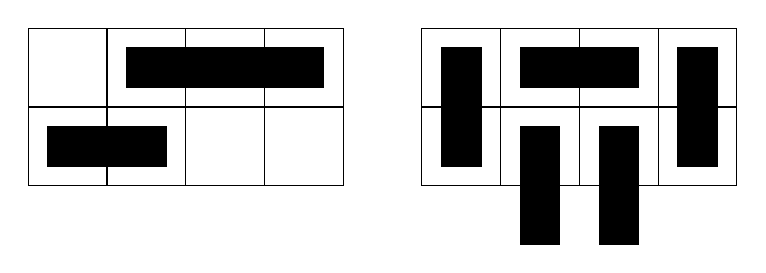
\begin{tikzpicture}[x=1.0cm, y=1.0cm]
        \foreach \y in {0,1} {
            \foreach \x in {0,...,3} {
                \draw (0+\x ,0+\y) rectangle ++ (1,1);
            }
        }

        \draw[fill, black] (0.25 ,0.25) rectangle ++ (1.5,0.5);
        \draw[fill, black] (1.25 ,1.25) rectangle ++ (1.5,0.5);
        \draw[fill, black] (2.25 ,1.25) rectangle ++ (1.5,0.5);

        \foreach \y in {0,1} {
            \foreach \x in {0,...,3} {
                \draw (5+\x ,0+\y) rectangle ++ (1,1);
            }
        }

        \draw[fill, black] (5+1.25 ,1.25) rectangle ++ (1.5,0.5);
        \draw[fill, black] (5+1.25 ,-0.75) rectangle ++ (0.5,1.5);
        \draw[fill, black] (5+2.25 ,-0.75) rectangle ++ (0.5,1.5);
        \draw[fill, black] (5+0.25 ,0.25) rectangle ++ (0.5,1.5);
        \draw[fill, black] (5+3.25 ,0.25) rectangle ++ (0.5,1.5);
    \end{tikzpicture}
\end{center}

与之前一样,先观察前几种情形($n = 1, 2, 3$ 等),尝试寻找规律。在继续阅读之前,建议先自行思考!

当 $n = 1$ 时,棋盘形状恰好与一块多米诺骨牌相同,因此仅有一种密铺方式。用 $T(n)$ 表示 $2 \times n$ 棋盘的密铺数,故 $T(1) = 1$。

\begin{center}
    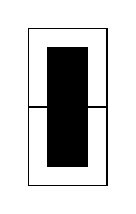
\begin{tikzpicture}[x=1.0cm, y=1.0cm]
        \draw (0,0) rectangle ++ (1,1);
        \draw (0,1) rectangle ++ (1,1);
        \draw[fill, black] (0.25 ,0.25) rectangle ++ (0.5,1.5);
    \end{tikzpicture}
\end{center}

当 $n = 2$ 时,$2 \times 2$ 棋盘有两种不同的密铺方式,此时棋盘的方向很重要,因此 $T(2) = 2$。

\begin{center}
    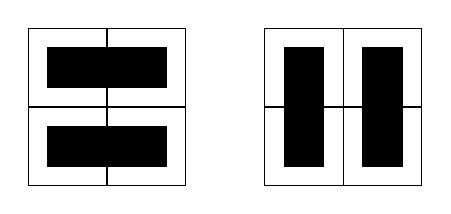
\begin{tikzpicture}[x=1.0cm, y=1.0cm]
        \foreach \y in {0,1} {
            \foreach \x in {0,1} {
                \draw (0+\x ,0+\y) rectangle ++ (1,1);
            }
        }

        \draw[fill, black] (0.25 ,0.25) rectangle ++ (1.5,0.5);
        \draw[fill, black] (0.25 ,1.25) rectangle ++ (1.5,0.5);

        \foreach \y in {0,1} {
            \foreach \x in {0,1} {
                \draw (3+\x ,0+\y) rectangle ++ (1,1);
            }
        }

        \draw[fill, black] (3+0.25 ,0.25) rectangle ++ (0.5,1.5);
        \draw[fill, black] (3+1.25 ,0.25) rectangle ++ (0.5,1.5);
    \end{tikzpicture}
\end{center}

当 $n = 3$ 时,通过枚举可得 $T(3) = 3$。

\begin{center}
    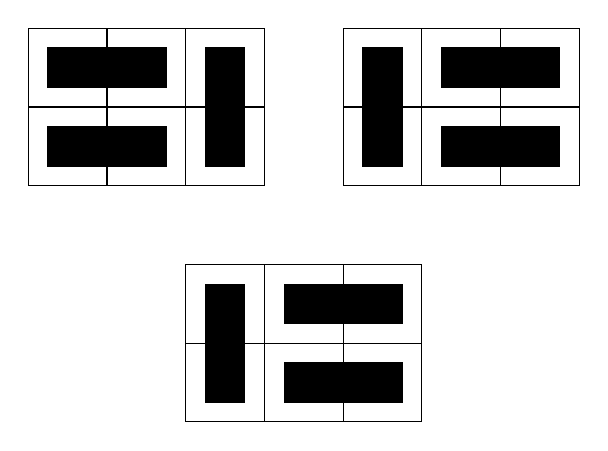
\begin{tikzpicture}[x=1.0cm, y=1.0cm]
        \foreach \y in {0,1} {
            \foreach \x in {0,1,2} {
                \draw (0+\x ,0+\y) rectangle ++ (1,1);
            }
        }

        \draw[fill, black] (0.25 ,0.25) rectangle ++ (1.5,0.5);
        \draw[fill, black] (0.25 ,1.25) rectangle ++ (1.5,0.5);
        \draw[fill, black] (2.25 ,0.25) rectangle ++ (0.5,1.5);

        \foreach \y in {0,1} {
            \foreach \x in {0,1,2} {
                \draw (4+\x ,0+\y) rectangle ++ (1,1);
            }
        }

        \draw[fill, black] (4+1.25 ,0.25) rectangle ++ (1.5,0.5);
        \draw[fill, black] (4+1.25 ,1.25) rectangle ++ (1.5,0.5);
        \draw[fill, black] (4+0.25 ,0.25) rectangle ++ (0.5,1.5);

        \foreach \y in {0,1} {
            \foreach \x in {0,1,2} {
                \draw (2+\x ,-3+\y) rectangle ++ (1,1);
            }
        }

        \draw[fill, black] (2+1.25 ,-3+0.25) rectangle ++ (1.5,0.5);
        \draw[fill, black] (2+1.25 ,-3+1.25) rectangle ++ (1.5,0.5);
        \draw[fill, black] (2+0.25 ,-3+0.25) rectangle ++ (0.5,1.5);
    \end{tikzpicture}
\end{center}

再看 $n=4$ 的情形,可验证 $T(4)=5$。

\begin{center}
    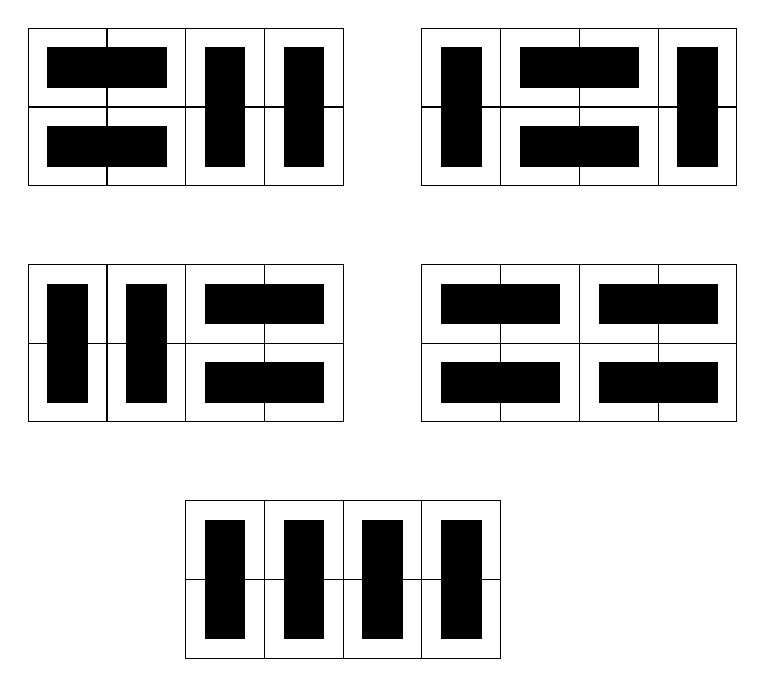
\begin{tikzpicture}[x=1.0cm, y=1.0cm]
        \foreach \y in {0,1} {
            \foreach \x in {0,...,3} {
                \draw (0+\x ,0+\y) rectangle ++ (1,1);
            }
        }

        \draw[fill, black] (0.25 ,0.25) rectangle ++ (1.5,0.5);
        \draw[fill, black] (0.25 ,1.25) rectangle ++ (1.5,0.5);
        \draw[fill, black] (2.25 ,0.25) rectangle ++ (0.5,1.5);
        \draw[fill, black] (3.25 ,0.25) rectangle ++ (0.5,1.5);

        \foreach \y in {0,1} {
            \foreach \x in {0,...,3} {
                \draw (5+\x ,0+\y) rectangle ++ (1,1);
            }
        }

        \draw[fill, black] (5+1.25 ,0.25) rectangle ++ (1.5,0.5);
        \draw[fill, black] (5+1.25 ,1.25) rectangle ++ (1.5,0.5);
        \draw[fill, black] (5+0.25 ,0.25) rectangle ++ (0.5,1.5);
        \draw[fill, black] (5+3.25 ,0.25) rectangle ++ (0.5,1.5);

        \foreach \y in {0,1} {
            \foreach \x in {0,...,3} {
                \draw (0+\x ,-3+\y) rectangle ++ (1,1);
            }
        }

        \draw[fill, black] (2.25 ,-3+0.25) rectangle ++ (1.5,0.5);
        \draw[fill, black] (2.25 ,-3+1.25) rectangle ++ (1.5,0.5);
        \draw[fill, black] (0.25 ,-3+0.25) rectangle ++ (0.5,1.5);
        \draw[fill, black] (1.25 ,-3+0.25) rectangle ++ (0.5,1.5);

        \foreach \y in {0,1} {
            \foreach \x in {0,...,3} {
                \draw (5+\x ,-3+\y) rectangle ++ (1,1);
            }
        }

        \draw[fill, black] (5+2.25 ,-3+0.25) rectangle ++ (1.5,0.5);
        \draw[fill, black] (5+2.25 ,-3+1.25) rectangle ++ (1.5,0.5);
        \draw[fill, black] (5+0.25 ,-3+0.25) rectangle ++ (1.5,0.5);
        \draw[fill, black] (5+0.25 ,-3+1.25) rectangle ++ (1.5,0.5);

        \foreach \y in {0,1} {
            \foreach \x in {0,...,3} {
                \draw (2+\x ,-6+\y) rectangle ++ (1,1);
            }
        }

        \draw[fill, black] (2+0.25 ,-6+0.25) rectangle ++ (0.5,1.5);
        \draw[fill, black] (2+1.25 ,-6+0.25) rectangle ++ (0.5,1.5);
        \draw[fill, black] (2+2.25 ,-6+0.25) rectangle ++ (0.5,1.5);
        \draw[fill, black] (2+3.25 ,-6+0.25) rectangle ++ (0.5,1.5);
    \end{tikzpicture}
\end{center}

现在能否寻找规律?手工计算更大棋盘的密铺数过于繁琐。尝试利用 $T(1) = 1$ 推导 $T(2)$……但无法实现,因为两情形本质不同:多米诺骨牌尺寸为 $2 \times 1$,仅添加一行不足以建立联系。

那么考虑 $n = 3$。能否利用 $T(2) = 2$?答案是肯定的!已知 $2 \times 2$ 棋盘有两种密铺,可直接将其扩展:在每种密铺右侧\emph{添加竖直多米诺骨牌},得到两种 $2 \times 3$ 密铺。但实际上 $T(3) = 3$,第三种密铺从何而来?观察发现,第三种密铺右侧为两块水平放置的多米诺骨牌。若移去这两块骨牌,剩余部分即 $n=1$ 的情形。换言之,第三种密铺是通过在 $2 \times 1$ 棋盘右侧\emph{添加两块水平骨牌}构成的。综上,$2 \times 3$ 棋盘的所有密铺均可由较小尺寸($2 \times 2$ 和 $2 \times 1$)导出:

\begin{center}
    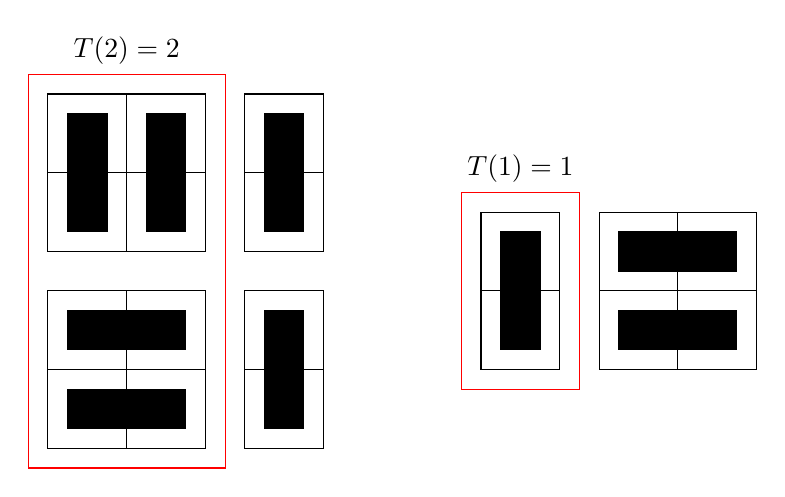
\begin{tikzpicture}[x=1.0cm, y=1.0cm]
        \foreach \g in {0, 2.5} {
            \foreach \y in {0,1} {
                \foreach \x in {0,1} {
                    \draw (0+\x ,0+\y+\g) rectangle ++ (1,1);
                }
            }
            \draw (2.5,0+\g) rectangle ++ (1,1);
            \draw (2.5,1+\g) rectangle ++ (1,1);
            \draw[fill, black] (2.75 ,0.25+\g) rectangle ++ (0.5,1.5);
        }

        \draw[fill, black] (0.25 ,0.25) rectangle ++ (1.5,0.5);
        \draw[fill, black] (0.25 ,1.25) rectangle ++ (1.5,0.5);

        \draw[fill, black] (0.25 ,2.5+0.25) rectangle ++ (0.5,1.5);
        \draw[fill, black] (1.25 ,2.5+0.25) rectangle ++ (0.5,1.5);

        \draw[red] (-0.25, -0.25) rectangle ++(2.5, 5);
        \path (-0.25,4.75) --  (2.25,4.75) node[midway,above,black] {$T(2)=2$};

        \draw (5.5,1) rectangle ++ (1,1);
        \draw (5.5,2) rectangle ++ (1,1);
        \draw[fill, black] (5.75 ,1.25) rectangle ++ (0.5,1.5);
        \draw[red] (5.25, 0.75) rectangle ++(1.5, 2.5);
        \path (5.25,3.25) --  (6.75,3.25) node[midway,above,black] {$T(1)=1$};

        \foreach \y in {0,1} {
            \foreach \x in {0,1} {
                \draw (7+\x ,1+\y) rectangle ++ (1,1);
            }
        }
        \draw[fill, black] (7.25 ,1.25) rectangle ++ (1.5,0.5);
        \draw[fill, black] (7.25 ,2.25) rectangle ++ (1.5,0.5);

    \end{tikzpicture}
\end{center}
\[T(3) = 3 = 2 + 1 = T(2) + T(1)\]

规律初现!再验证 $n = 4$:向 $T(3)$ 的每种密铺添加竖直骨牌,或向 $T(2)$ 的每种密铺添加两块水平骨牌,即可得到 $T(4)$ 的\emph{所有}密铺:

\begin{center}
    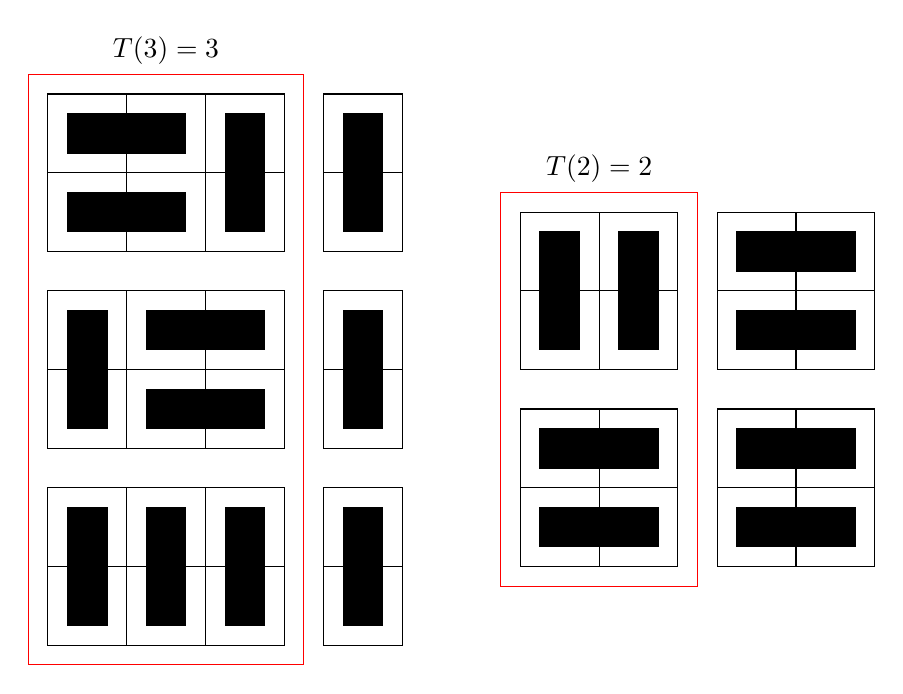
\begin{tikzpicture}[x=1.0cm, y=1.0cm]
        \foreach \g in {0, 2.5, 5} {
            \foreach \y in {0,1} {
                \foreach \x in {0,1,2} {
                    \draw (0+\x ,0+\y+\g) rectangle ++ (1,1);
                }
            }

            \draw (3.5,\g+0) rectangle ++ (1,1);
            \draw (3.5,\g+1) rectangle ++ (1,1);
            \draw[fill, black] (3.75 ,\g+0.25) rectangle ++ (0.5,1.5);
        }
        \draw[fill, black] (0.25 ,0.25) rectangle ++ (0.5,1.5);
        \draw[fill, black] (1.25 ,0.25) rectangle ++ (0.5,1.5);
        \draw[fill, black] (2.25 ,0.25) rectangle ++ (0.5,1.5);

        \draw[fill, black] (0.25 ,2.75) rectangle ++ (0.5,1.5);
        \draw[fill, black] (1.25 ,2.75) rectangle ++ (1.5,0.5);
        \draw[fill, black] (1.25 ,3.75) rectangle ++ (1.5,0.5);

        \draw[fill, black] (2.25 ,5.25) rectangle ++ (0.5,1.5);
        \draw[fill, black] (0.25 ,5.25) rectangle ++ (1.5,0.5);
        \draw[fill, black] (0.25 ,6.25) rectangle ++ (1.5,0.5);

        \draw[red] (-0.25, -0.25) rectangle ++(3.5, 7.5);
        \path (-0.25,7.25) --  (3.25,7.25) node[midway,above,black] {$T(3)=3$};


        \foreach \g in {0, 2.5} {
            \foreach \y in {0,1} {
                \foreach \x in {0,1} {
                    \draw (6+\x ,1+\y+\g) rectangle ++ (1,1);
                }
            }
            \foreach \y in {0,1} {
                \foreach \x in {0,1} {
                    \draw (8.5+\x ,1+\y+\g) rectangle ++ (1,1);
                }
                \draw[fill, black] (8.75 ,1.25+\g+\y) rectangle ++ (1.5,0.5);
            }
           
        }

        \draw[fill, black] (6.25 ,1.25) rectangle ++ (1.5,0.5);
        \draw[fill, black] (6.25 ,2.25) rectangle ++ (1.5,0.5);

        \draw[fill, black] (6.25 ,3.5+0.25) rectangle ++ (0.5,1.5);
        \draw[fill, black] (7.25 ,3.5+0.25) rectangle ++ (0.5,1.5);

        \draw[red] (5.75, 0.75) rectangle ++(2.5, 5);
        \path (5.75,5.75) --  (8.25,5.75) node[midway,above,black] {$T(2)=2$};
        
    \end{tikzpicture}
\end{center}
\[T(4) = 5 = 3 + 2 = T(3) + T(2)\]

需要注意的是,此方式不会产生重复密铺。(仔细思考为何能保证唯一性?)由此可直接推出 $T(4) = T(3) + T(2)$。

此外,上述论证具有普适性。对于任意 $n$,观察棋盘最右侧:若为竖直骨牌,则密铺源于 $2 \times (n - 1)$ 棋盘;若为水平骨牌对,则源于 $2 \times (n-2)$ 棋盘。因此对所有满足条件的 $n$ 有:
\[T(n) = T(n - 1) + T(n - 2)\]
哪些 $n$ 值适用?请记住,我们必须单独分析 $T(1)$ 和 $T(2)$;因此上述公式不适用于 $n=1$ 和 $n=2$,我们必须添加限制条件 $n \ge 3$ 才能使上面公式成立。

据此可轻松计算任意 $n$ 对应的 $T(n)$,甚至可编程实现。但正是\emph{归纳}论证——对模式的细致观察及其成因的透彻分析——使我们得出最终结论。本例中,$T(n)$ 的值依赖于前两项 $T(n-1)$ 和 $T(n-2)$,这在前文示例中\emph{未曾}出现,这暗示了更深层的机制。是否察觉此前的归纳定义与多米诺骨牌类比在此失效?如何修正类比以解释此情况?思考一下这些问题,然后再继续阅读。我们将在下一个示例之后深入讨论它们。

顺便一提,你是否注意到此数列的特别之处?你还知道其他类似的数列吗?思考一下吧……


% !TeX root = ../../../book.tex
\subsection{制胜策略}

这个例子将是我们第一个\emph{无需}证明数值公式的归纳问题!这似乎很奇怪,但正如即将看到的那样,这却是一个事实。实际上在数学中,这比你想象的更常见:一个问题或数学对象可能存在某些潜在的归纳结构,但却不依赖代数或算术的内容。

事实上,我们将讨论一个\emph{游戏}。就是通常意义上的游戏——有两个玩家必须遵守的规则,并且有明显的赢家和输家——同时也是数学意义上的游戏,我们可以使用数学符号来制定规则和游戏情境,并以抽象的方式讨论\emph{策略}。我们甚至可以\emph{解}这个游戏。这与棒球比赛非常不同。

现在让我们讨论一下这个游戏的规则,我们暂时将其称为``取石子''。有两个玩家,称为 $P_1$ 和 $P_2$。玩家 $P_1$ 先行。玩家面前的桌子上有两堆石子,每堆正好有 $n$ 个石子,其中 $n$ 是某个自然数。(为了区分游戏的不同版本,当每堆石子有 $n$ 个石子时,我们会说玩家正在``玩 $T_n$''。)在每个玩家的回合中,他们可以从\emph{任意}一堆中取走\emph{任意}数量的石子。但不能同时从两堆石子中取石子。取走\emph{最后}一颗石子的玩家\emph{获胜}。

试着跟朋友玩一下这个游戏。使用硬币或糖果当石子。再试着切换一下角色,你先作为 $P_1$,然后再作为 $P_2$。尝试制定一个获胜\emph{策略},一种最大化获胜机会的游戏方法。尝试猜测不同的 $n$ 值下会发生什么。谁``应该''获胜?你能\emph{证明}吗?说真的,在继续阅读我们的分析之前,先玩玩这个游戏并尝试证明一些结论。你可能会对自己所取得的成就感到惊讶!

与其他示例一样,让我们使用 $n$ 的一些较小值来弄清楚到底发生了什么,然后再尝试进行泛化。当 $n = 1$ 时,这个游戏相当愚蠢。$P_1$ 必须取走其中一堆中唯一的石子,然后 $P_2$ 取走另一堆中唯一剩余的石子。因此,$P_2$ 胜。(请注意,无论 $P_1$ 选择两堆中的哪一堆,$P_2$ 总是会得到另一堆。我们可以说``不失一般性'', $P_1$ 选择左边这堆,因为无论选择哪一堆都无关紧要;情况是等价的,所以为了方便具体讨论,我们不妨说是左边这堆。后面讨论数理逻辑时,我们也会深入探讨``不失一般性''这一思想。)


\begin{center}
    \begin{tikzpicture}[line width=0.5mm]
        \foreach \n in {0, 1}{
            \node at (\n, 0)[circle,fill,inner sep=8pt, anchor=west]{};
            \draw (\n, -1) -- +(0.8, 0);
        }
        \draw[-latex] (2.5, -0.4) -- +(2, 0) node[midway,above]{$P_1$ 回合};
        \draw (5, -1) -- +(0.8, 0);
        \node at (6, 0)[circle,fill,inner sep=8pt, anchor=west]{};
        \draw (6, -1) -- +(0.8, 0);
        \draw[-latex] (7.5, -0.4) -- +(2, 0) node[midway,above]{$P_2$ 回合};
        \draw (10, -1) -- +(0.8, 0);
        \draw (11, -1) -- +(0.8, 0);
        \path (10, -0.4) -- +(2, 0) node[midway,above]{$P_2$ 胜!};
    \end{tikzpicture}
\end{center}

当 $n = 2$ 时,可能会出现几种情况。思考 $P_1$ 可能采取的行动。同样地,$P_1$ 可能选择左堆也可能选择右堆,但因为最终结果是相同的,并且我们可以交换这两堆,所以我们可以说(不失一般性)$P_1$ 从左堆取走若干石子。具体是多少?可能是一颗石子也可能是两颗石子。让我们分别检验每种情况。

\begin{center}
    \begin{tikzpicture}[line width=0.5mm]
        \foreach \x in {0, 1}{
            \node at (\x, 0)[circle,fill,inner sep=8pt, anchor=west]{};
            \node at (\x, 1)[circle,fill,inner sep=8pt, anchor=west]{};
            \draw (\x, -1) -- +(0.8, 0);
        }
        \draw[-latex] (2.5, -0.4) -- +(2, -0.6);
        \draw[-latex] (2.5, 0.6) -- +(2, 0.6);
        \node[anchor=west] at(2.5,0) {$P_1$ 回合};
        \foreach \delta in {1, -2}{
            \foreach \n in {0, 1}{
                \draw (5+\n, \delta) -- +(0.8, 0);
                \node at (6, \delta+1+\n)[circle,fill,inner sep=8pt, anchor=west]{};
            }
        }
        \node at (5, -1)[circle,fill,inner sep=8pt, anchor=west]{};
        \draw[-latex] (7.5, 2) -- +(2, 0) node[midway,above]{$P_2$ 回合};
        \draw[-latex] (7.5, -1) -- +(2, 0) node[midway,above]{$P_2$ 回合};
        \draw (10, 1) -- +(0.8, 0);
        \draw (11, 1) -- +(0.8, 0);
        \path (10, 1.6) -- +(2, 0) node[midway,above]{$P_2$ 胜!};
        \path (10, -1.4) -- +(2, 0) node[midway,above]{???};
    \end{tikzpicture}
\end{center}

如果 $P_1$ 取走两颗石子,$P_2$ 应该如何应对呢?$P_2$ 可以取走另一堆从而获胜,所以 $P_1$ 一开始就不应该采取这一行动。不过,可能 $P_1$ 脑子不清什么的,而且我们需要考虑所有可能的情况来全面分析这场比赛。因此,在这种情况下(上图中的上半行)$P_2$ 获胜。好吧,这就是简单的情况。

如果 $P_1$ 只从左边一堆石子(上图中的下半行)中取走一颗石子怎么办?$P_2$ 应该如何应对?我们现在有几种选择:

\begin{itemize}
    \item 如果 $P_2$ 从左边一堆石子中取走另一颗石子……那么,$P_2$ 取走另一堆全部石子,$P_1$ 获胜。
    \item 如果 $P_2$ 从右边一堆石子中取走全部两颗石子……那么,$P_1$ 取走左边一堆中的最后一颗石子,$P_1$ 获胜。
    \item 然而,如果 $P_2$ 只从右边一堆石子中取走一颗石子……
\end{itemize}

\begin{center}
    \begin{tikzpicture}[line width=0.5mm]
        \foreach \g in {0, 5, 10} {
            \foreach \x in {0, 1} {
                \node at (\x+\g, 0)[circle,fill,inner sep=8pt, anchor=west]{};
                \draw (\x+\g, -1) -- +(0.8, 0);
            }
        }
        \node at (0, 1)[circle,fill,inner sep=8pt, anchor=west]{};
        \node at (1, 1)[circle,fill,inner sep=8pt, anchor=west]{};
        \draw[-latex] (2.5, -0.4) -- +(2, 0) node[midway,above]{$P_1$ 回合};

        \node at (6, 1)[circle,fill,inner sep=8pt, anchor=west]{};
        \draw[-latex] (7.5, -0.4) -- +(2, 0) node[midway,above]{$P_2$ 回合};
    \end{tikzpicture}
\end{center}
现在我们遇到了与 $T_1$ 完全相同的情况,我们已经对此进行了分析!这次又是 $P_1$ 先走的,所以我们知道会发生什么:无论如何 $P_2$ 都会获胜。如果你是玩家 $P_2$,这显然是最好的应对:\emph{无论} $P_1$ \emph{如何行动},你都会赢!

退一步,让我们思考一下这表明了什么:无论 $P_1$ 首先采取什么行动(从任一堆中取走一个或两个石子),$P_2$ 都可以做出\emph{某个可能的回应,保证} $P_2$ 总会获胜,无论 $P_1$ 随后采取什么回应。哇,$P_2$ 稳坐钓鱼台!让我们看看其他 $n$ 值的情况下是否会发生同样的事情。

当 $n = 3$ 时,我们将再次假设(不失一般性)玩家 $P_1$ 从左边石子堆上取石子。他可以取走一颗、两颗或三颗石子:

\begin{itemize}
    \item 如果 $P_1$ 取走全部三颗,那么 $P_2$ 就会完全拿走另一堆并获胜。
    \item 如果 $P_1$ 取走两颗石子……那么 $P_2$ 应该做什么呢?
\end{itemize}
取完左边一堆是愚蠢的(因为 $P_1$ 可以取走整个右边一堆从而获胜),而取走整个右边一堆也同样愚蠢(因为 $P_1$ 可以取走整个左边一堆从而获胜),所以需要介于两者之间。现在,如果 $P_2$ 仅从右侧一堆石子中取走一颗石子,请注意 $P_1$ 可以采用相同的动作做出回应;从而使得两堆石子都只剩下一颗,但先手互换了。在这种情况下,$P_2$ 先行,根据我们之前的分析,$P_2$ 肯定会输。因此这是糟糕的策略!

\begin{center}
    \begin{tikzpicture}[line width=0.5mm]
        \foreach \g in {0, 5, 10, 15}{
            \foreach \x in {0, 1}{
                \node at (\x+\g, 0)[circle,fill,inner sep=8pt, anchor=west]{};
                \draw (\x+\g, -1) -- +(0.8, 0);
            }
        }
        \foreach \x in {0, 1, 6}{
            \foreach \y in {0, 1}{
                \node at (\x, \y)[circle,fill,inner sep=8pt, anchor=west]{};
                \node at (\x, \y+1)[circle,fill,inner sep=8pt, anchor=west]{};
            }
        }

        \node at (11, 1)[circle,fill,inner sep=8pt, anchor=west]{};

        \draw[-latex] (2.5, -0.4) -- +(2, 0) node[midway,above]{$P_1$ 回合};
        \draw[-latex] (7.5, -0.4) -- +(2, 0) node[midway,above]{$P_2$ 回合};
        \draw[-latex] (12.5, -0.4) -- +(2, 0) node[midway,above]{$P_1$ 回合};
        \path (15, 0.6) -- +(2, 0) node[midway,above]{$P_1$ 胜!};
    \end{tikzpicture}
\end{center}

让我们再试一次。如果 $P_2$ 从右边一堆石子中取走两颗石子……瞧!现在,我们每堆中只有一颗石子,$P_1$ 先行,所以我们知道  $P_1$ 一定会输。$P_2$ 再次完胜!

\begin{center}
    \begin{tikzpicture}[line width=0.5mm]
        \foreach \g in {0, 5, 10}{
            \foreach \x in {0, 1}{
                \node at (\x+\g, 0)[circle,fill,inner sep=8pt, anchor=west]{};
                \draw (\x+\g, -1) -- +(0.8, 0);
            }
        }
        \foreach \x in {0, 1, 6}{
            \foreach \y in {0, 1}{
                \node at (\x, \y)[circle,fill,inner sep=8pt, anchor=west]{};
            }
        }
        \draw[-latex] (2.5, -0.4) -- +(2, 0) node[midway,above]{$P_1$ 回合};
        \draw[-latex] (7.5, -0.4) -- +(2, 0) node[midway,above]{$P_2$ 回合};
        \path (10, 0.6) -- +(2, 0) node[midway,above]{$P_2$ 胜!};
    \end{tikzpicture}
\end{center}

思考一下 $n = 4$ 的情况,你会发现完全相同的分析再次出现。你会考虑另一种可能性:玩家 $P_1$ 可以从左边一堆石子中取走一颗、两颗、三颗或四颗。不过,无论 $P_1$ 怎么做,你都会发现 $P_2$ 可以在另一堆上\emph{模仿}相同的动作,将整个游戏简化为之前的\emph{较小}版本,从而保证 $P_2$ 一定获胜!看起来 $P_2$ 一直处于主导地位,因为他可以对 $P_1$ 的任何行为做出回应,在另一堆上做出相同的动作。无论 $P_1$ 做什么,$P_2$ 总会做出回应,这意味着 $P_2$ 一定获胜,无论 $P_1$ 随后的动作是什么。从这个意义上讲,我们说``$P_2$ 有制胜策略''。$P_2$ 有一个清晰且可描述的方法来评估比赛局势并选择特定的行动来\emph{保证获胜}。

我们要如何证明这一点?如何应用本章的归纳法?目前可能很难看出来。我们在这里到底要证明什么?对这个问题的类比中,多米诺骨牌或阶梯是什么?在你开动脑筋思考这个例子时,你应该意识到以下几点:归纳法并不总是与代数式有关;归纳法代表某种``构建''结构,较大的情况依赖于较小的情况;我们必须证明一些初始事实,然后论证如何化简任意更大事实,使其依赖于先前的事实。这才是多米诺骨牌类比的真正目的。碰巧的是,这个类比可以很好地解释某些归纳问题(但不是全部),并且是可视化的,令人印象深刻。但它并不完全适用于\emph{所有}情况。

回顾本章的四个例子,思考它们有何相似之处和不同之处。 尝试使用一些更好的术语(也许是你自己发明的)对数学归纳法进行更精确的数学描述。(这里的意思是比直观的类比更好。你会惊讶地发现,在不真正知道自己``应该''说什么的情况下,你竟然能够很好地描述归纳法,并且在这个过程中你会学到很多东西!)在适当的时候,我们会对数学归纳法及其各种形式进行严格的陈述和证明。与此同时,我们需要探索数学的一些其他领域,以建立必要的语言、符号和知识,以便回过头解决这个问题。不过,在开始之前,我们应该了解一下数学归纳法的一些有用的应用。


% !TeX root = ../../../book.tex
\subsection{习题}

\subsubsection*{温故知新}

以口头或书面的形式简要回答以下问题。这些问题全都基于你刚刚阅读的内容,如果忘记了具体定义、概念或示例,可以回顾相关内容。确保在继续学习之前能够自信地作答这些问题,这将有助于你的理解和记忆!

\begin{enumerate}[label=(\arabic*)]
    \item 如何\emph{归纳}这两个例子?它们与立方体、直线的例子在哪些方面相似?在哪些方面不同?
    \item 对于多米诺骨牌密铺问题,计算 $T(n)$ 需要知道前几项值?
    \item $T(n) = T(n - 1) + T(n - 2)$ 与 $T(n + 2) = T(n + 1) + T(n)$ 有什么区别?
    \item 取石子游戏的必胜策略是什么?请与不了解策略的朋友试玩,并采用玩家 $P_2$ 的必胜策略。观察你每次获胜时对方的反应如何?对方是否开始察觉这一策略?
\end{enumerate}

\subsubsection*{小试牛刀}

尝试解答以下问题。这些题目需动笔书写或口头阐述答案,旨在帮助你熟练运用新概念、定义及符号。题目难度适中,确保掌握它们将大有裨益!

\begin{enumerate}[label=(\arabic*)]
    \item $T(5)$ 的值是多少?能否画出所有密铺方案?
    \item 分析两堆各 $4$ 颗石子的取石子游戏:玩家 $P_2$ 是否总有必胜策略?
    \item \textbf{挑战题:}若使用\emph{三堆}等量石子进行游戏,会如何发展?能否为任意一方找到必胜策略?不妨与朋友实际对弈,观察结果!
    \item 探索\emph{斐波那契数列}:它与多米诺骨牌密铺问题中的数列 $T(n)$ 有何关联?
\end{enumerate}

\newpage
% !TeX root = ../../../book.tex
\section{应用}

% !TeX root = ../../../book.tex
\subsection{递归程序}\label{sec:section2.5.1}

数学归纳法背后的概念在计算机科学中有着广泛应用。回想我们推导 $\sum_{k=1}^{n}k^2$ 公式的过程:一旦找到用较小立方和及剩余项表示立方数的方法,就会反复进行替换,直到抵达最初观察到的``最简''情况——即计算起点 $2^3=1+3+3+1$。递归编程正是运用了这一思想:通过确定``大''问题如何依赖``小''案例来简化问题,直至达到已知的简单案例。

此类技术的经典示例是计算\emph{阶乘} $n!$ 的代码,其定义为前 $n$ 个自然数的乘积:
\[n! = 1 \cdot 2 \cdot 3 \dots (n - 1) \cdot n\]
这个定义对人类而言直观易懂,但指导计算机执行该乘积却并非易事(尝试思考:如何在代码中表达``持续执行直至达到 $n$''?)。实际上,更有效的函数编程方法以及对数学归纳定义的建模,是让程序\emph{递归调用自身}直至``最简''情况。对于阶乘而言,该情况即 $1! = 1$。对于任意其他 $n$ 值,可反复应用关系:
\[n! = (n - 1)! \cdot n\]
来计算 $n!$。以下\emph{伪代码}体现了这一思想:

\begin{verbatim}
    factorial(n):
        if n = 1
            return 1
        else
            return n * factorial(n-1)
    end
\end{verbatim}

我们已知 $1! = 1$,若需计算此值,将直接返回正确结果。对于任意 $n > 1$,程序会调用\emph{自身}:``请计算 $(n-1)!$,然后乘以 $n$ 得到答案。''为计算 $(n-1)!$,程序再次检查输入是否为 $1$;若不为 $1$,则继续调用自身:``请计算 $(n-2)!$,然后乘以 $(n-1)$。''此过程持续至程序返回 $1! = 1$。随后,程序便能计算 $2! = 1 \times 2$,进而 $3! = 2! \times 3$,依此类推,最终得到 $n! = (n - 1)! \times n$。

\clearpage

递归编程的另一个经典例子是\emph{斐波那契数列}。你可能在数学课上见过这个数列(事实上,我们在上一节讨论多米诺骨牌密铺时提到过它),或者听说过它以有趣而奇妙的方式出现在自然界中——该数列最早由意大利比萨数学家莱昂纳多·斐波那契 (Leonardo Fibonacci) 在研究兔子种群增长时``发现''。斐波那契数列的前两项均为 $1$,后续每一项都定义为前两项之和。若用 $F(n)$ 表示第 $n$ 个斐波那契数,则有:
\[F(1) = 1 \text{\ 且\ }F(2) = 1, \text{ 对于任意\ } n \ge 3, F(n) = F(n - 1) + F(n - 2)\]
那么,$F(5)$ 等于多少?$F(100)$ 或 $F(10000)$ 呢?递归程序可以轻松解决这个问题。思路一致:当函数遇到基本情况 $F(1)$ 或 $F(2)$ 时,直接返回 $1$;否则,递归调用自身计算前两项并求和。阅读以下伪代码并思考其工作原理:若用此程序计算 $F(10)$,过程会如何展开?

\begin{verbatim}
    Fibonacci(n):
        if n = 1 or n = 2
            return 1
        else
            return Fibonacci(n-1) + Fibonacci(n-2)
    end
\end{verbatim}

该程序与 \verb|factorial| 函数思路相似(通过递归调用计算更小规模的问题直至达到已知解),但蕴含更深层的机制。若输入 $n = 10$,程序发现结果未知,将调用自身计算 \verb|Fibonacci(9)| 和 \verb|Fibonacci(8)|。每次调用遇到未知值时,又会触发新的递归计算——例如为求 $F(9)$ 需计算 $F(8)$ 和 $F(7)$,而为求 $F(8)$ 又需计算 $F(7)$ 和 $F(6)$。这导致相同输入值被多次重复计算。

请比较 \verb|Fibonacci| 与 \verb|factorial| 程序,思考它们如何体现归纳过程的核心思想。两者是否采用类似策略?与介绍数学归纳法时用到的``多米诺骨牌''类比有何关联?不妨将骨牌 $n$ 的``事实''视为 $n!$ 的正确计算或 $F(n)$ 的值,这个类比在两种情况下如何成立?所有骨牌是否必然倒下?在继续阅读之前,请带着这些问题深入思考——其背后蕴藏着强大的数学基础。

\clearpage


% !TeX root = ../../../book.tex
\subsection{汉诺塔}

我们休息一下,玩个游戏吧。其实不完全是休息,因为从某种意义上来说,这是一个\emph{归纳}游戏,所以是完全相关的。但好歹是个游戏!\emph{汉诺塔}是一个非常受欢迎的智力游戏,部分原因在于它的规则和设备都很简单。不过解决这个问题却一点也不简单!

想象一下,我们有三个垂直的杆和三个不同尺寸(\textcolor{blue}{蓝色}、\textcolor{olivegreen}{绿色}和\textcolor{red}{红色})的圆盘,彼此叠放在一起,如下所示:

\begin{center}
    \begin{tikzpicture}[line width=4mm,line cap=round,xscale=3,brown!30]
        \def\sequence{3/1,2/1,1/1}
        % init colors
        \foreach[count=\j] \c in {red,olivegreen,blue}
            \gset col[\j]={\c};
        \edef\numdisks{\j}
        % init positions and draw support
        \foreach \j in {1,2,3}{
            \gset pos[\j]=0
            \draw (\j,-.4) -- +(0,3);
        }
        \draw (.5,-.4) -- +(3,0);

        % draw
        \foreach[count=\k] \i/\j in \sequence{
            \edef\delta{\i*0.4/3}
            \draw[draw={\get col[\i]}](\j-\delta,\get pos[\j]) -- (\j+\delta,\get pos[\j]);
            \ginc pos[\j]+={.4}
        }
    \end{tikzpicture}
\end{center}
目标是通过遵循以下规则将所有三个圆盘移动到另一根杆上(无论是中间的还是右边的,都没关系):

\begin{enumerate}
    \item 每次移动只能将一根杆子顶部的一个(且\emph{仅有}一个)圆盘,移动到另一根杆子的顶部,
    \item 任何圆盘不能放置在比它小的圆盘之上。
\end{enumerate}
就这些!两条简单的规则,但却是一个很难的游戏。尝试用一些硬币或扑克牌或任何你手边的东西来模拟这个游戏。(你甚至可以在一些游戏商店购买汉诺塔套装。)你能解决这个问题吗? 你花了多少步?你的解决方案是``最好''的吗?为什么是或者为什么不是呢?

我们提到过这是一个归纳游戏,所以让我们探讨一下这个想法。我们想要解决这个难题需要多少步(其中一步表示一个圆盘从一根杆移动到另一根杆),更具体地说,确定解决这个难题所需的\emph{最小可能步数}。对于三个圆盘的问题,如果我们愿意的话,完全可以不断地在两根杆之间来回移动最小圆盘并产生 $100$ 次移动,然后再解决它,但这肯定不是最好的方法,对吗?假设我们找到了一种在一定步数内解决问题的方法;我们如何证明我们使用的步数是最小可能步数?

为了解决这个问题,我们想\emph{递归地}分解解题方法。在此过程中,我们实际上要回答一个更普遍的问题:解决 $3$ 根杆上 $n$ 个圆盘的汉诺塔问题需要的最小移动步数是多少?我们仅用 $3$ 个圆盘提出了问题,是为了便于为你提供一个具体的版本供你思考和使用,但我们可以通过深入思考来回答这个更普遍的问题。为了确保我们理解一致,我们将向你展示如何解决具有 $3$ 个圆盘的问题:

\begin{center}
    \begin{tikzpicture}[line width=2.6mm,line cap=round,xscale=1.5,yscale=0.5,brown!30]
        \def\sequencelist{{3/1,2/1,1/1}, {3/1,2/1,1/3}, {3/1,2/2,1/3}, {3/1,2/2,1/2}, {3/3,2/2,1/2}, {3/3,2/2,1/1}, {3/3,2/3,1/1}, {3/3,2/3,1/3}}
        % init colors
        \foreach[count=\j] \c in {red,olivegreen,blue}
            \gset col[\j]={\c};
        \edef\numdisks{\j}
        \foreach[count=\n] \sequence in \sequencelist {
            % init positions and draw support
            \foreach \j in {1,2,3}{
                \gset pos[\j]=0
                \draw (\j,-0.4-5*\n) -- +(0, 3);
            }
            \draw (0.5,-0.52-5*\n) -- +(3,0);
            % draw
            \foreach[count=\k] \i/\j in \sequence{
                \edef\delta{\i*0.4/3}
                \draw[draw={\get col[\i]}](\j-\delta,\get pos[\j]-5*\n) -- (\j+\delta,\get pos[\j]-5*\n);
                \ginc pos[\j]+={0.52}
            }
        }
        \node[black,left] at (0,-5.52){开始};
        \foreach \m in {1, ..., 7} {
            \node[black,left] at (0,-5.52-5*\m){第 \m 步};
        }   
    \end{tikzpicture}
\end{center}

请注意,最大的圆盘对于大多数解决方案来说基本上是``无关''的。由于我们可以在其上面放置任何其他圆盘,因此我们需要做的就是通过将其他圆盘移动到不同的杆上来``露出''该圆盘,将最大的圆盘移动到唯一的空杆上,然后再将其他圆盘移到大圆盘上。本质上,我们执行相同的过程(将两个较小的圆盘从一根杆移动到另一根杆)两次,在两次之间,我们将大圆盘从一根杆移动到另一根杆。如果最大的圆盘根本不存在,那么我们实际做的就是 $2$ 个圆盘的题目,只是做了两次!(仔细思考这一点,确保你理解了上面这段话。假装大的\textcolor{blue}{蓝色}圆盘不存在,操作一遍上图中步骤。)

这表明解决 $3$ 盘问题的方法涉及解决 $2$ 盘问题的两次迭代,中间有一次额外的移动(移动最大的圆盘)。一般来说,这表明了解决该问题的\emph{递归}过程。为了最优地解决 $n$ 盘问题,我们只需遵循解决 $(n - 1)$ 盘问题的最优过程,用一步移动最大的第 $n$ 个圆盘,然后再次求解 $(n - 1)$ 盘问题。

现在我们对如何最优地解决这个问题有了一些了解,让我们确定该过程需要几步。认识到解决这个问题需要使用\emph{递归}算法,我们意识到\emph{证明}有关最佳解决方案的任何内容都需要\emph{归纳法}。因此,我们需要为我们的多米诺骨牌线确定一个``起点'',它应该对应于问题的``最小''或``最简单''版本。对于汉诺塔问题来说,最简问题就是 $1$ 个圆盘问题。当然,这几乎不是一个``问题'',因为我们可以一步解决它,只需将唯一的圆盘从一根杆移动到另一根杆即可。如果我们令 $M(n)$ 表示解决 $n$ 盘问题所需的最少移动次数,那么我们就确定了 $M(1) = 1$。为了确定 $M(2)$,我们可以使用上面的观察结果并得到
\[\underbrace{M(2)}_{2 \text{盘问题}}= \underbrace{M(1)}_{1 \text{盘问题}}+ \underbrace{1}_{\text{移动最大盘}}+ \underbrace{M(1)}_{1 \text{盘问题}}= 1 + 1 + 1 = 3\]
接下来一定是
\[M(3) = M(2) + 1 + M(2) = 3 + 1 + 3 = 7\]
和
\[M(4) = M(3) + 1 + M(3) = 7 + 1 + 7 = 15\]
以此类推。你注意到其中的规律了吗?这些数字中的每一个都比 $2$ 的幂小 $1$,具体来说,我们注意到对于迄今为止我们所考察的每种情况,$M(n) = 2^n - 1$。需要指出的是,观察到这种规律并不等于证明了这种规律;因为它仅仅适用于前 $4$ 种情况,并不意味着这种规律会一直持续下去,而这正是归纳证明所要解决的问题。此外,认识到这种规律并``观察''到 $M(n) = 2^n - 1$ 本身就是一件了不起的事情。我们碰巧知道答案,并且可以直接找出公式。你可以尝试自己``解决''以下关系
\[M(n) = 2M(n - 1) + 1 \text{ 且 } M(1) = 1\]
看看能否推导出公式 $M(n) = 2^n -1$。这种公式比上面的关系式更好的原因在于,$M(n)$ 仅取决于 $n$,而\emph{不再}取决于之前的项(例如 $M(n-1)$)。这种关系和其他类似关系被称为\emph{递归关系},一般来说,它们可能很难解决!

我们知道如何解决这个问题,并得出 $M(n) = 2^n - 1$。不过,相关的验证工作就留给你独立完成。你可以通过检查上面等式中的一些值来做到这一点,但我们都知道这并不构成\emph{证明}。尝试通过归纳步骤来实际证明这一点!我们已经完成了大部分工作,但还需你仔细、清晰地将一切串联在一起。请记住,你应该确定每张多米诺骨牌上的``事实''是什么,确保多米诺骨牌 $1$ 会倒下,然后对多米诺骨牌 $n$ 倒下会引起多米诺骨牌 $(n+1)$ 倒下进行一般论证。试着写出这个证明。这些细节对你来说有意义吗?向朋友展示你的证明,看看他们是否理解。你还需要告诉他们其他事情或指导他们完成证明阅读?考虑解释你的方法和步骤的最佳方式,以便书面版本就足够了,而不必添加任何口头解释。思考\emph{解释}你的方法和步骤的最佳方式,确保书面版本足够清晰准确,而不必添加任何口头解释。 


% !TeX root = ../../../book.tex
\subsection{习题}

\subsubsection*{温故知新}

以口头或书面的形式简要回答以下问题。这些问题全都基于你刚刚阅读的内容,所以如果忘记了具体的定义、概念或示例,可以回去重读相关部分。确保在继续学习之前能够自信地回答这些问题,这将有助于你的理解和记忆!

\begin{enumerate}[label=(\arabic*)]
    \item 递归程序如何归纳?
    \item 汉诺塔的归纳结构是什么?在解决 $3$ 盘问题时,我们在哪里解决了 $2$ 盘问题?
\end{enumerate}

\subsubsection*{小试牛刀}

尝试回答以下问题。这些题目要求你实际动笔写下答案,或(对朋友/同学)口头陈述答案。目的是帮助你练习使用新的概念、定义和符号。题目都比较简单,确保能够解决这些问题将对你大有帮助!

\begin{enumerate}[label=(\arabic*)]
    \item 按照伪代码 \verb|factorial| 的步骤计算 $5!$。
    \item 按照伪代码 \verb|Fibonacci| 的步骤计算 $F(5)$。
    \item 解决 $4$ 盘汉诺塔问题。确保你能以\emph{最优}步数 $2^4 - 1 = 15$ 步完成。
\end{enumerate}

\newpage
% !TeX root = ../../../book.tex
\section{总结}

我们已经看到了一些\textbf{归纳证明}的例子。我们意识到我们正在解决的一些问题使用了类似的证明风格,并探索了几个例子来了解这些证明中可能出现的不同问题。具体来说,我们看到归纳证明\emph{并不}总是证明求和公式或方程:归纳证明适用于\emph{任何}依赖于该事实的``先前事实''的情况。这导致我们从数学角度对归纳法的工作原理进行了类比。目前,我们最喜欢用``多米诺骨牌类比''来思考归纳法,但我们接下来的主要目标之一是严格\emph{陈述}和\emph{证明}归纳法原理。现在,让我们对这种类型的证明进行大量练习。这就是本章习题的目的。稍后,一旦我们将归纳正式化,我们能会更好地使用归纳法,并且我们会对这一概念有更透彻的理解!

\newpage
% !TeX root = ../../../book.tex
\section{本章习题}

以下是一些问题,帮助你熟悉归纳式证明。我们不需要完全严格的证明,只要你能很好地描述过程并写下步骤即可。等我们掌握了数学归纳原理 (PMI) 和相应的证明策略后,再回头来严格证明这些问题。

\begin{exercise} \label{exc:exercises2.7.1}
    证明以下求和公式对于每个自然数都成立,对于 $n=0$ 也成立。
    \[\sum_{i=0}^{n}2^i=2^{n+1}-1\]
    后续问题:用这个结果来说明在 $2^n$ 支球队的单赛淘汰赛中需要进行多少场比赛才能确定获胜者。(例如,NCAA 疯狂三月锦标赛就使用这种赛制,其中 $n = 6$。)
\end{exercise}

\begin{exercise}
    证明对于每个大于等于 $2$ 的自然数 $n$, $3^n \ge 2^{n+1}$。
\end{exercise}

\begin{exercise}
    对于哪些自然数 $n$,下列不等式成立?先陈述结论,然后再证明它。
    \begin{enumerate}
        \item $2^n \ge (n + 1)^2$
        \item $2^n \ge n!$
        \item $3^{n+1} > n^4$
        \item $n^3 + (n + 1)^3 > (n + 2)^3$
    \end{enumerate}
\end{exercise}

\begin{exercise}
    \textbf{末日游戏}:两名玩家轮流从日历中命名日期。每一回合中,玩家可以增加月份或日期,但不能同时增加。起始位置为 1 月 1 日,说出 12 月 31 日的人获胜。确定第一个玩家的必胜策略。
    例如,玩家 1 获胜的一系列动作如下:
    \begin{itemize}
        \item 玩家 1: 1 月 10 日;
        \item 玩家 2: 3 月 10 日;
        \item 玩家 1: 8 月 10 日;
        \item 玩家 2: 8 月 25 日;
        \item 玩家 1: 8 月 28 日;
        \item 玩家 2: 11 月 28 日;
        \item 玩家 1: 11 月 30 日;
        \item 玩家 2: 12 月 30 日;
        \item 玩家 1: 12 月 31 日。
    \end{itemize}
    我们所说的\emph{必胜}策略是指玩家 1 遵循的一种游戏方法,无论玩家 2 做什么,都可以\emph{保证}获胜。
\end{exercise}

\begin{exercise}
    找到并证明\emph{几何级数}求和公式,几何级数定义如下:
    \[\sum_{i=0}^{n-1}q^i\]
    其中 $q$ 为实数,$n$ 为自然数。(提示:留意 $q = 1$ 的情况。)
\end{exercise}

\begin{exercise}
    写一个依赖于 $n$ 的句子,使得该句子对于从 $1$ 到 $99$(含)的所有 $n$ 值都为真,但当 $n = 100$ 时该句子为假。
\end{exercise}

\begin{exercise}
    下面``错误证明''证明了对于所有 $n$, $a^n=1$。请指出问题在哪里?
    \begin{spoof}
        设 $a$ 为非零实数。请注意 $a^0 = 1$。另请注意我们可以归纳地写出
        \[a^{n+1} = a^n \cdot a = a^n \cdot \frac{a^n}{a^{n-1}} = 1 \cdot \frac{1}{1} = 1\]
    \end{spoof}
\end{exercise}

\begin{exercise}
    未来社会中,只有两种面额的货币:一种价值 $3$ Brendan 的硬币,一种价值 $8$ Brendan 的硬币。还有一项全国性法令,店主只能收取可以使用这两种硬币\textbf{精确支付}的价格。

    店主可能向你收取的一杯咖啡的法定价格是多少?
    
    \textbf{提示:}尝试一些较小的值,看看会发生什么。
\end{exercise}

\begin{exercise}
    对于某个任意自然数 $n$,考虑大小为 $2^n \times 2^n$ 的棋盘。从棋盘上移除\textbf{任意}一个方格。 是否可以用 L 形三联骨牌来密铺剩余的方格?

    如果你的答案是肯定的,请证明这一点。

    如果您的答案是否定的,请提供反例论证。(也就是说,找到一个 $n$ 使得任何方法都无法密铺棋盘,并说明为什么会出现这种情况。)
\end{exercise}

\begin{exercise}
    考虑一个 $n \times n$ 的正方形网格。该网格内存在多少个任意大小的子方格?例如,当 $n = 2$ 时,答案为 $5$:有 $4$ 个$1 \times 1$ 方格和 $1$ 个 $2 \times 2$ 方格。找到你的答案的公式并尝试证明它是正确的。
\end{exercise}

\begin{exercise}
    证明,在至少有 $2$ 人的队列中,如果第一个人是女性,最后一个人是男性,那么在队列的某个位置一定存在一个男性紧邻女性身后。
\end{exercise}

\begin{exercise}
    对于每个自然数 $n$,证明 $n^3 - n$ 是 3 的倍数。
\end{exercise}

\begin{exercise}
    \textbf{二进制 $n$ 元组}是由 \verb|0| 和 \verb|1| 组成的有序字符串,字符串中共有 $n$ 个数字。提供一个\emph{归纳论证}来解释为什么有 $2^n$ 个可能的二进制 $n$ 元组。
\end{exercise}

\begin{exercise}
    回想一下,\textbf{斐波那契数}是通过设 $f_0 = 0$ 和 $f_1 = 1$,然后对于每个 $n \ge 2$,设 $f_n = f_{n-1} + f_{n-2}$ 来定义的。这会产生序列 $0, 1, 1, 2, 3, 5, 8, 13, 21, 34, \dots$

    你可能不知道,斐波那契数列也有\emph{封闭形式};也就是说,除了上面给出的常规递归定义外,还有一个特定\emph{公式}来定义它。那就是:
    \[f_n = \frac{1}{\sqrt 5}\Bigg[\Bigg(\frac{1+\sqrt 5}{2}\Bigg)^n - \Bigg(\frac{1-\sqrt 5}{2}\Bigg)^n\Bigg]\]
    证明该公式对于所有 $n \ge 0$ 都正确。
\end{exercise}

\begin{exercise}
    再次考虑斐波那契数 $f_n$,证明以下内容:
    \begin{enumerate}
        \item $\displaystyle{\sum_{i=0}^{n}f_i = f_{n+2} - 1}$
        \item $\displaystyle{\sum_{i=0}^{n}f_i^2 = f_n \cdot f_{n+1}}$
        \item $\displaystyle{f_{n-1} \cdot f_{n+1} - f_n^2 = (-1)^n}$
        \item $\displaystyle{f_{m+n} = f_n \cdot f_{n+1} + f_{m-1} \cdot f_n}$
        \item $\displaystyle{f_n^2 + f_{n+1}^2 = f_{2n+1}}$
    \end{enumerate}
\end{exercise}

\begin{exercise}
    尝试提供一个归纳论证来解释为什么每个 $n ≥ 2$ 的自然数都可以写成质数的乘积。你能证明该乘积的\emph{唯一性}吗?也就是说,你能解释为什么\emph{只有唯一一种方法}可以将自然数分解为质数吗?
\end{exercise}

\begin{exercise}
    证明
    \[\sum_{k=1}^{n} k \cdot k! = 1 \cdot 1! + 2 \cdot 2! + 3 \cdot 3! + \dots + n \cdot n! = (n+1)!-1\]
\end{exercise}

\clearpage

\begin{exercise}
    下面的``错误证明''得出所有的笔颜色都一样,问题出在哪儿?
    \begin{spoof}
        考虑一组数量为 $1$ 的笔。由于只有 $1$ 支笔,所以它的颜色肯定与自身相同。

        假设任意一组 $n$ 支笔在组内只有一种颜色。(注意:我们已经解释了为什么这个假设对于 $n = 1$ 是有效的,所以我们可以做出这个假设。)取任意一组 $n + 1$ 支笔。将它们排列在桌子上,从左到右用 $1$ 到 $n + 1$ 编号。查看其中的前 $n$ 个,即查看笔 $1,2,3, \dots , n$。这是一组 $n$ 支笔,因此根据假设,该组只有一种颜色。(我们还不知道是什么颜色。)然后,查看最后 $n$ 支笔;即查看笔 $2,3, \dots ,n+1$。这也是一组 $n$ 支笔,因此根据假设,该组也只有一种颜色。而 $2$ 号笔恰好属于这两个组。因此,无论 $2$ 号笔的颜色是什么,这也是\dotuline{两组}中每支笔的颜色。因此,所有 $n+1$ 支笔具有相同的颜色。

        根据归纳法,这表明任何一组笔,无论多少,都只有一种颜色。那么,纵观世界上有限的钢笔,我们应该只能找到一种颜色。
    \end{spoof}
\end{exercise}

\begin{exercise}
    $\star$ 这题\emph{极其难解},摘自著名数学家陶哲轩(Terence Tao)的博客(\href{https://terrytao.wordpress.com/2011/04/07/the-blue-eyed-islanders-puzzle-repost/}{详见链接})

    有一座岛屿,岛上居住着一个部落。这个部落有 $1000$ 人,有着不同颜色的眼睛。然而,他们的宗教信仰禁止他们知道自己眼睛的颜色,甚至禁止讨论这个话题;因此,每个居民都可以(并且确实可以)看到所有其他居民眼睛的颜色,但无法知道自己眼睛的颜色(不考虑反射表面)。如果部落成员确实发现了自己眼睛的颜色,那么他们的宗教信仰就会迫使他们第二天中午在村庄广场举行自杀仪式,让所有人围观。所有的部落成员都是高度逻辑和虔诚的,他们都知道其他人也是高度逻辑和虔诚的(并且他们都知道他们都知道其他人是高度逻辑和虔诚的,等等)。

    (就这个逻辑谜题而言,``高度逻辑的''意味着能够从岛民可用的信息和观察中逻辑推断出的任何结论,该岛民将自动知晓。)

    事实证明,在这 $1000$ 名岛民中,有 $100$ 人是蓝眼睛,$900$ 人是棕眼睛,尽管岛民最初并没有意识到这些统计数据(当然,他们每个人只能看到 $1000$ 名部落居民中的 $999$ 人)。

    一天,一名蓝眼睛的外国人来到岛上,并赢得了部落的完全信任。

    一天晚上,他向整个部落发表讲话,感谢他们的热情款待。

    然而,由于不了解当地习俗,这名外国人在称呼中错误地提及了眼睛的颜色,并表示\emph{在世界的其他角落看到另一个像我这样的蓝眼睛的人是多么不同寻常}。

    这种失礼(如果有的话)会对部落带来什么影响?
\end{exercise}

\newpage
% !TeX root = ../../../book.tex
\section{展望}

在本章中,我们向你介绍了\textbf{数学归纳法}的概念。我们看了一些示例,其中归纳过程指导了我们的解题思路,然后我们描述了如何通过\emph{归纳证明}来\emph{严格验证}该解题思路。凭借迄今为止我们掌握的数学技术和概念,我们必须依靠非技术性的类比来向你描述这个过程。某种程度上,这就像让朋友向你描述如何挥高尔夫球杆,即使你以前从未打过高尔夫球。当然,它们可以为你提供一些关于挥杆``感受就像是什么''的心理想象,但如果不亲自练习,你如何真正理解高尔夫挥杆的机制呢?如何学习怎样调整你的挥杆动作,或辨别一号木杆、五号铁杆和沙坑挖起杆之间的区别呢?通过研究底层机制并刻意练习,我们希望更好地理解数学归纳法,以便将来我们可以适当地使用它,识别它适用的情况,并最终学习如何使其\emph{适应}其他情况。当然,记住多米诺骨牌的类比会有助于引导我们的直觉,但我们也应该记住,这不是严格的数学。它也不能完美地描述我们讨论的其中几个例子,在这些例子中,倒下的多米诺骨牌不仅取决于紧随其后的多米诺骨牌,还取决于它之前的其他几张多米诺骨牌。

在下一章中,我们将探讨严格陈述和证明数学归纳法作为证明技术所需的一些相关概念。具体来说,我们将研究\emph{数理逻辑}的一些思想,研究如何将复杂的数学陈述和定理分解为更小的组成部分,以及如何从基本构建模块中构建起有趣且复杂的陈述。在此过程中,我们将引入一些新的符号和速记符,使我们能够将一些冗长的陈述压缩成简洁(且精确)的数学语言。有了这些之后,我们将探索一些更基本的证明策略,然后将其应用于本课程中\emph{所做的所有其他事情},包括归纳技术本身!我们还将研究\emph{集合论}的一些思想,集合论是数学的一个分支,构成了所有其他分支的基础。这对于将来组织我们的想法非常有用,而它也将帮助我们以严格的方式定义\emph{自然数}。有了这两个数学分支的一些概念和知识,我们就可以在坚实的基础上建立数学归纳法,并继续正确地使用它。
% !TeX root = ../../book.tex
\chapter[集合]{集合:数学的基石}\label{ch:chapter03}

% !TeX root = ../../../book.tex
\section{引言}

现在是时候学习集合了!这部分内容出现在上一章之后,似乎是一个奇怪的跳跃。请详细我们,这是自然且必要的。我们在数学中所做的一切都建立在集合的基础上,所以我们最好现在就开始学习集合并习惯使用集合。

% !TeX root = ../../../book.tex
\subsection{目标}

以下简短内容将向你展示本章如何融入本书的体系。这部分内容会描述我们之前的工作将如何发挥作用,还会激发我们为什么要研究本章出现的主题,并告诉你我们的目标,以及你在阅读时应该记住什么来实现这些目标。现在,我们将通过一系列陈述为你总结本章的主要目标,以及本章结束时你应该获得的技能和知识。以下各节将更详细地重申这些想法,但这里将为你提供一个简短的列表以供将来参考。当学完本章后,请返回此列表,看看你是否理解所有这些目标。你明白为什么我们在这里概述它们很重要吗?你能定义我们使用的所有术语吗?你能应用我们描述的技术吗?

\textbf{学完本章后,你应该能够……}

\begin{itemize}
    \item 定义什么是集合,并给出几个常见的例子。
    \item 使用正确的符号来定义集合并引用其元素。
    \item 定义并描述常见集合操作;即用两个或多个集合创建新集合的方法。
    \item 描述如何比较两组两个集合,并应用恰当的技术来证明此类观点。
    \item 解释自然数与集合的关系,并将其与数学归纳法联系起来。
\end{itemize}


% !TeX root = ../../../book.tex
\subsection{承上}

我们正在构建数学归纳法的正式表述,并将其证明为\emph{定理}。为了实现这一目标,我们需要一些基本对象以便于逻辑严谨地处理和讨论。集合就是那些对象!从历史上看,数学是在二十世纪初才建立在\emph{集合论}的基础之上。在那之前,数学家们倾向于对他们工作背后真正发生的事情``撒手不管''。他们做出了很多``直觉上的''假设,但从未尝试严格且\emph{公理化地}描述他们所做的一切。数学家\textbf{乔治·康托尔(Georg Cantor)}的工作向大家展示了一些令人惊讶且反直觉的结果,这些结果完全正确且与我们的假设一致……于是,我们意识到我们有必要确定我们一直谈论的内容。当然,这并不是要抹黑 1900 年之前的数学家的工作!我们只是说他们一直在玩一个游戏,但并没有真正就一套规则达成一致。这就是集合论\textbf{公理体系}。


% !TeX root = ../../../book.tex
\subsection{启下}

我们的核心动机是不断学习\textbf{证明},理解其本质与运作方式,特别是严谨的数学归纳法。更广泛地说,我们对数学家的实际工作充满兴趣。我们确信,任何数学家都会强调\textbf{集合}在其研究中的重要性。他们或许会表示自己不愿从事纯\emph{集合论}工作,但无人能否认集合的基础地位。

后续所有讨论都将涉及对特定对象集合的陈述。我们将尝试断言(并证明)某些对象具有特定性质。定义这些对象需要集合语言,而表述这些断言则需要数学逻辑——这是我们即将学习的内容。当前首要任务是掌握各类数学对象的表达方式,方能对其进行准确描述。


% !TeX root = ../../../book.tex
\subsection{忠告}

本章将引入若干新颖的数学概念,不同于前两章专注于数字、代数、算术及批判性思维的谜题。这些新思想需要专注阅读并积极思考。学习概念与结论时,请仔细研读并深入反思。数学文本比报刊文章对读者要求更高:它期待你\emph{全神贯注},斟酌每句话的含义,必要时暂停数分钟以确保真正理解。请谨记:阅读数学虽有挑战,但这很正常!不必气馁,将每句话视为整体拼图的关键部分。

若本章的研读时间(含课堂学习时间)等同甚至超过前两章的总和,这不足为奇。根据我们长期以来的观察,最具挑战的往往是集合的\textbf{表示法}。这可能是你首次被要求如此\textbf{精确}而\textbf{严谨}地书写。仅``思路正确''是不够的;我们必须确保文字准确反映思想。完成问题或作业后,请反复检查并自问:``此表述是否合理?是否准确传达了我的本意?读者能否据此理解我的思想?''

此外,本章涉及比常规数学课程更\textbf{抽象}的思维。无论你是否感到吃力,都不可能速读求成。此时更需投入时间消化:精读几页后,在用餐、散步等日常活动中反复思考;寻找现实中的实例;与同伴探讨集合概念。这或许看似多余,但终将使你获益匪浅。请相信我们的经验。


\newpage
% !TeX root = ../../book.tex
\section{``集合''思想}

\subsubsection*{``物以类聚''}

集合的直观概念对你来说可能并不陌生。如果你奥特曼卡收藏者\footnote{原作这里用的是``棒球明星卡'',考虑到中国读者对棒球运动的陌生,译者将其改成风靡中国(青少年界)的奥特曼卡。--- 译者注},拥有``全套''卡片意味着拥有发行商发行的某个系列的每一张卡。如果你和朋友一起玩桌游,你们会在玩之前商定一套``规则'',这样以后就不会出现未解决的争议。如果你在生物、化学或物理课上进行了实验室实验,你会将数据收集到``数据集''中并分析这些结果以检验假设。

这是三种不同情况,每种情况都涉及单词``集或套''(\textbf{set}),那么该单词是如何关联上下文并赋予正确含义的呢?本质上,集合是指基于某些共同属性而组织在一起的对象的全体。在第一个示例中,稀有度为 UR 的每一张卡都属于该特定集合。在第二个示例中,任何商定好的规则都将属于规则集合。在第三个示例中,实验中收集的任何数据都属于该数据集。在每种情况下,都有一个共同的属性,让我们可以将特定对象彼此关联起来,并将它们作为一个集合来引用。

\subsubsection*{数学中的集合}

集合在数学中非常常见、非常流行、同时也非常有用、非常基础。因为数学家研究的是抽象对象以及这些对象之间的关系,因此如果无法引用一组数学对象,就很难准确描述所思考的内容。事实上,我们已经不自觉地用到了集合!

例如,在研究多项式和二次函数求根公式时,我们提到具有负判别式(当 $\frac{b^2}{4a} - c < 0$ 时)的二次多项式 $p(x) = ax^2 + bx + c$ \emph{在实数集中}没有根。我们想表达什么?你理解这句话吗?我们试图传达这样的想法:无论我们从所有实数的集合中选择哪个实数 $x$,都可以保证 $p(x) \ne 0$。但是实数地集合到底是什么?它是如何定义的?我们怎么能确定它存在呢?实际上这是相当难回答的问题,尝试解答这些问题会让我们远离集合论的世界。

在数学的语言中,我们的目标是使我们的句子和陈述\emph{准确无误},并寻求基于某些基本假设来建立真理。我们需要以这些假设为起点,否则我们就没有任何真理为基础。这些假设,就像每个人在``玩数学游戏''之前都同意其成为``规则集合''的一部分,被称为\textbf{公理}。

如果你学过一些几何或者读过希腊数学家欧几里得(Euclid)和他的名著《\emph{几何原本}》,那么你可能对``公理''一词不陌生。欧几里得\emph{证明}的所有基本几何结论都建立在几个基本假设之上:任意两点都可以用线段连接,必须存在给定中心点和半径的圆,非平行线相交,等等。这些陈述一开始就被认为是真的。

\textbf{集合论}作为一个重要的数学分支也构建在公理之上。集合论的公理体系为所有涉及集合的结论打下了坚实的基础,利用这些公理和由公理推导出来的结果,我们可以继续发现数学宇宙中新的真理。不过,研究这些公理及其推论更适合专门讨论集合论的课程,我们这里把集合论公理的许多推论视为理所当然,而无需严格证明它们。这并不是因为不能证明,而仅仅是因为这些证明需要占用本书太多时间和篇幅来完成。

我们\emph{要}做的是提供一个``集合''的定义,满足我们在本书中使用集合的上下文需求。我们还将定义集合的一些基本属性,分享一些说明性示例,并讨论集合上创建新集合的不同操作。



\newpage
% !TeX root = ../../../book.tex
\section{定义与示例}

% !TeX root = ../../../book.tex
\subsection{``集合''的定义}

让我们从定义开始。正如前文解释的那样,集合的特征在于其包含的对象分组以及定义该集合的属性。以下定义旨在精确化这一概念,同时引入相关符号与术语。

\begin{definition}
     \textbf{集合}是具有共同明确定义属性的所有对象组成的全体。集合中的对象称为集合的\textbf{元素}。数学符号 ``$\in$'' 表示``是……的元素''(``$\notin$'' 表示``不是……的元素'')。
\end{definition}


% !TeX root = ../../../book.tex
\subsection{示例}

我们通过具体示例(包括集合与非集合)来阐释集合的定义。数学中通常用大写字母表示集合,小写字母表示元素,我们遵循这一惯例(但非绝对)。定义集合需要明确其元素的共同属性。例如,定义 $B$ 为 NBA(美国职业篮球联赛)\footnote{原作这里用的是``MLB 美国职业棒球大联盟'',考虑到中国读者对棒球运动的陌生,译者将其改成了 NBA。—— 译者注}所有球队的集合。这是明确定义的属性吗?给定任意对象,能否明确判断其是否具有该属性?答案是肯定的,因此这构成一个合法集合。(为避免混淆,特指 2023 赛季的 NBA 球队。)数学表达为:
\[B = \{\text{2023\ 赛季所有\ NBA\ 球队}\}\]
``花括号'' \{ 和 \} 表示它们之间的描述构成一个集合。此时可表述为 $\text{洛杉矶湖人队} \in B$ 而 $\text{多伦多哈士奇} \notin B$。

符号 $\in$ 在汉语中常读作``是……的元素''、``是……的成员''、``属于……''或``在……中''。我们首选``是……的元素'',因为它足够明确,并且恰当地使用了数学术语``\textbf{元素}''。根据上下文的不同,可以适当使用其他等效说法,但不推荐。(尤其避免使用``在……中'',以防与其他集合关系混淆)。

以下为常见数集示例(你或许曾经使用过这些数字但从未以集合视角看待它们):
\begin{align*}
    \mathbb{N} &= \{ \text{自然数集} \} = \{1, 2, 3, \dots\}\\
    \mathbb{Z} &= \{ \text{整数集} \} = \{\dots , -2, -1, 0, 1, 2, \dots\}\\
    \mathbb{Q} &= \{ \text{有理数集} \} = \{ \text{能够写成\ } \frac{a}{b} \text{\ 形式的数,其中\ } a, b \in Z \text{\ 且\ } b \ne 0 \}\\
    \mathbb{R} &= \{ \text{实数集}\}
\end{align*}
思考 $\mathbb{Q}$ 的第二种定义为何合理。后文将展示更简洁的集合表示法。值得注意的是,$\mathbb{R}$ 的定义在此未具体展开——你能尝试定义实数吗?


% !TeX root = ../../../book.tex
\subsection{如何定义集合}

定义或描述集合的另一种方法是直接列出其所有元素。当集合元素数量较少时,这种方法十分简便。例如,集合 $V$ 的以下定义都是等价的:
\begin{align*}
    V &= \{A,E,I,O,U\}\\
    V &= \{\text{英语中的元音}\}\\
    V &= \{U,E,I,A,O\}
\end{align*}
``等价''意味着虽然上述定义使用了不同表述,但都确定了\emph{相同的}集合 $V$。(注意:我们约定 $y$ 为辅音,故 $y \notin V$。)元素 $A, E, I, O, U$ 的共同属性在于它们都是元音(如第二个定义所示)。由于仅有五个元素,完整列举既简单又便捷(如第一个定义所示)。

\subsubsection*{顺序和重复无关紧要}

第三个定义为何与其他定义等价?因为它指代相同的元素整体——集合完全由其元素决定,因此元素的\emph{顺序无关紧要}。$U \in V$ 是否成立?答案是``肯定的'',无论 $U$ 位于列表的位置。

不仅元素顺序无关,元素的\emph{重复}也不影响集合的性质!集合 $A=\{a,a,a\}$ 与 $A=\{a\}$ 完全相同。集合的本质仅取决于其元素内容(我们将在 \ref{sec:section3.4.4} 节``口袋类比''中再次讨论)。$A = \{a, a, a\}$ 仅表示 $a \in A$ 重复三次,而 $A$ 实际仅含唯一元素 $a$。因此 $A = \{a\}$ 是最简洁的表述方式。

\subsubsection*{元素自身可构成共同属性}

延续通过列举元素定义集合的思路,考虑集合 $A$:
\[A=\{2, 7, 12, 888\}\]
这显然是一个集合。但元素间的共同属性是什么?元音集合 $V$ 可辅以语言描述,而 $A$ 似乎仅能罗列元素。数学上,$2,7,12,888$ 的共同属性恰恰是它们都属于集合 $A$!在抽象领域中,仅通过定义集合 $A$ 本身便赋予其元素共同属性。这合理吗?你能否找到\emph{另一个}明确定义的共同属性来精确生成 $A$ 的元素?(提示:构造多项式 $p(x)$ 使其根恰好为 $2,7,12,888$。)若元素具有多重关联属性,你认为选择哪一属性定义集合重要吗?如何理解集合 $S := \{2, 7, \text{M}, \text{波士顿凯尔特人队}\}$?除``同属此集合''外,它们是否存在其他共同属性?

\subsubsection*{省略号可用但非正式方法}

当集合定义无歧义或已通过其他方式明确定义时,可以列举示例元素并用省略号压缩元素列表。例如:
\[E = \{\text{所有偶数}\} = \{2, 4, 6, 8, 10, \dots\}\]
事实上,此集合为\emph{无限集},无法穷举所有元素,但前几项已清晰表明指代偶数集,且主定义 $E$ 为``所有偶数的集合''已明确其含义。需要强调的是,此方法并非精确的数学定义,仅适用于非正式场合。下一小节讨论集合的正规定义方法时,我们将进一步阐明这一点。

\subsubsection*{集合建构式符号}

定义或描述集合的最佳方法是将其元素限定为具有特定属性的另一个集合的元素。例如,若希望表示 $1$ 到 $100$(含)之间所有自然数的集合 $S$,虽可列出所有元素,但这过于冗长。也可使用省略号法 $S = \{1, 2, 3, \dots , 100\}$,但此方式缺乏正式定义,仍不够精确(不同读者可能对省略号有不同理解)。更精确且简洁的写法是:
\[S = \{x \in \mathbb{N} \mid 1 \le x \le 100\}\]
我们将此式理解为``$S$ 是自然数集 $\mathbb{N}$ 中所有满足 $1 \le x \le 100$ 的元素 $x$ 构成的集合''。

竖线符号 $\mid$ 表示``\textbf{满足}'',其左侧指定对象来自哪个``更大集合'',右侧描述对象应满足的属性。

(\textcolor{red}{注意}:\emph{请勿}在其他场景下用 $\mid$ 表示``满足''。该符号仅在定义集合时作为分隔符使用,用以区分左侧的元素来源集与右侧的属性描述。)

这是广泛使用的\textbf{集合建构式符号}示例。其核心在于从``更大''集合中\emph{筛选}具有特定属性的元素来\emph{构建}新集合,为此需要明确:
\begin{enumerate}[label=(\arabic*)]
    \item 更大集合是什么;
    \item 共同属性是什么。
\end{enumerate}

让我们用几个例子进一步说明:
\begin{align*}
    S &= \{x \in \mathbb{N} \mid 1 \le x \le 100\} = \{1, 2, 3, \dots , 100\} \\
    T &= \{z \in \mathbb{Z} \mid \text{存在某\ } k \in \mathbb{Z} \text{\ 使得\ } z = 2k\} = \{\dots , -4, -2, 0, 2, 4, \dots\} \\
    U &= \{x \in \mathbb{R} \mid x^2 - 2 = 0\} = \{-\sqrt{2}, \sqrt{2}\}\\
    V &= \{x \in \mathbb{N} \mid x^2 - 2 = 0\}= \{ \}
\end{align*}

最后两个例子凸显出上下文的重要性:当改变元素来源的\emph{更大集合}时,相同的属性条件($x^2 -2 = 0$)会产生不同的集合。该条件在实数范围内有两个解,但在自然数范围内无解!是否存在满足该条件的有理数?请思考。

这就解释了为何必须明确指定更大集合。类似``$U = \{x \mid x^2 - 2 = 0\}$''的定义\emph{没有意义},因其存在歧义,可能导致完全不同的解释。

\subsubsection*{朗读建构式符号}

我们正在学习一门新的\textbf{语言},前述内容涵盖基本词汇与语法规则。需要通过练习将这些数学表达式转化为汉语(在脑海中大声朗读),反之亦然。例如,可将集合 $S$ 合理定义为以下任一形式:
\begin{itemize}
    \item $S$ 是所有满足 $1 \leq x \leq 100$ 的自然数 $x$ 的集合。
    \item $S$ 是介于 $1$ 到 $100$(含端点)之间的全体自然数的集合。
    \item $S$ 是满足不等式 $1 \leq x \leq 100$ 的自然数 $x$ 的集合。
    \item $S$ 是满足 $1 \le x \le 100$ 属性的自然数 $x$ 的集合。
\end{itemize}
请注意,这些定义均通过指定更大集合与共同性质来限定元素;其差异仅在语言表述层面,数学本质完全一致。

请尝试为其他集合撰写类似定义。可收集他人对集合的口头描述,并将其转化为数学符号。

回顾有理数集 $\mathbb{Q}$ 的定义,可将其重写为:
\begin{align*}
    \mathbb{Q} &= \Big\{\frac{a}{b}, \text{其中\ } a,b \in \mathbb{Z} \text{\ 且\ } b \ne 0\Big\}\\
               &= \Big\{x \in \mathbb{R} \mid \text{存在\ } a, b \in \mathbb{Z} \text{\ 使得\ } \frac{a}{b}= x \text{\ 且\ } b \ne 0\Big\}
\end{align*}
请注意这两个定义的细微差别:前者强调有理数呈现 $\frac{a}{b}$ 的\textbf{形式}并限定参数条件;后者则表明有理数是满足特定性质的实数,可以表示为整数之比。后者更受青睐,因为它提供了更丰富的信息。

一般来说,若 $P(x)$ 表示明确定义的性质(自然语言或数学语言),$X$ 为给定集合,则符号
\[S = \{x \in X \mid P(x)\}\]
读作
\begin{center}``$S$ 是集合 $X$ 中所有满足性质 $P(x)$ 的元素 $x$ 的集合''。\end{center}
在符号 $P(x)$ 中,字母 $x$ 表示变量对象,根据我们输入 $x$ 的特定对象,属性 $P(x)$ 可能成立(即 $P(x)$ 为真)也可能不成立(即 $P (x)$ 为假)。若性质成立,则我们将 $x$ 包含在 $S$ 中(因此 $x \in S$);若不成立,则我们将 $x$ 排除在 $S$ 外(因此 $x \notin S$)。

以偶数集 $E$ 为例,其精确定义为:
\begin{align*}
    E &= \{\text{偶数}\} \\
      &= \{x \in \mathbb{N} \mid \text{存在自然数\ } n \text{\ 使得\ } x = 2n\}
\end{align*}
请注意,此处存在两层性质判定:自然数 $x$ 属于 $E$ 当且仅当存在另一自然数 $n$ 满足 $x = 2n$。请尝试为奇数集、平方数集、质数集、回文数集、完美数集等构造类似定义。你能否运用集合构造器为这些集合建立精确的数学表达?


% !TeX root = ../../../book.tex
\subsection{空集}

如果没有元素满足性质 $P(x)$,会发生什么?例如,考虑定义
\[S = \{x \in \mathbb{N} \mid x^2 - 2 = 0\}\]
我们知道满足该性质的数 $x$ 是 $\sqrt{2}$ 和 $-\sqrt{2}$,但 $\sqrt{2} \notin \mathbb{N}$。因此,无论取 $\mathbb{N}$ 中的哪个元素 $x$,性质 $P(x)$(即 $x^2 - 2 = 0$)都不成立。这表明该集合不包含任何元素。这样的对象是否构成集合?

集合完全由其元素决定,没有元素的集合则通过``无元素''这一特性定义。若尝试列出其元素,可写作 $\{\}$。这个特殊的集合被称为空集:

\begin{definition}
    空集是没有元素的集合,记作 $\varnothing$。
\end{definition}

尽管用集合建构式符号定义空集的方式多种多样,但它们本质相同(注意:空集唯一存在!)。上文已展示一例,以下是其他例子:

\begin{align*}
    &\{a \in \mathbb{N} \mid a < 0\} \\
    &\{r \in \mathbb{R} \mid r^2 < 0\} \\
    &\{q \in \mathbb{Q} \mid q^2 \notin \mathbb{Q}\}
\end{align*}
你能理解为何这些定义均对应同一个空集吗?

\subsubsection*{上下文相关}

在集合建构式符号定义中,明确限定元素来源的集合 $X$ 至关重要。例如:
\begin{align*}
    S_1 &= \{x \in \mathbb{N} \mid |x| = 5\} = \{5\}\\
    S_2 &= \{x \in \mathbb{R} \mid |x| = 5\} = \{-5, 5\}
\end{align*}

(注意:使用下标区分同名集合是常见做法。)

此处限定范围直接影响结果,导致两个完全不同的集合。因此定义集合时必须精确清晰。类似 $S = \{x \mid |x| = 5\}$ 的表述因缺乏上下文而不严谨。


% !TeX root = ../../../book.tex
\subsection{罗素悖论}\label{sec:section3.3.5}

也许本节的内容看上去有点鸡蛋里挑骨头,但我们这样做背后的原因植根于集合论的一些基本思想。我们希望避免在没有这项规则的情况下可能出现的一些复杂问题和悖论。有一个十分著名的集合论悖论说明了为什么我们会有此需求,问题出在当我们使用集合构建符时,我们必须指定一个更大的集合。这个悖论被称为\emph{罗素悖论}(以英国数学家伯特兰·罗素(Bertrand Russell)命名),我们将在本节中介绍和讨论它。

\subsubsection*{集合的集合}

首先,我们需要指出,本节讨论将引入集合也可以是其他集合的元素的概念。这貌似是一个怪异且牵强的抽象想法,但它是数学中的一个基本概念。
举个具体的例子,回想一下所有 NBA 球队的集合 $B$。我们也可以将每个球队视为一个集合,其中的元素是球队中的球员。因此,可以说
\[\text{勒布朗·詹姆斯} \in \text{洛杉矶湖人队} \in B\]
因为 $\text{勒布朗·詹姆斯}$ 是集合 $\text{洛杉矶湖人队}$ 的元素,而 $\text{洛杉矶湖人队}$ 本身又是集合 $B$ 的元素。(但是请注意,$\text{勒布朗·詹姆斯} \notin B$。``$\in$'' 所表示的关系不具有\textbf{传递性}。我们将在后面定义这些术语。现在,我们说 ``$\le$'' 在实数集上表示的关系具有传递性。如果我们知道 $x \le y \le z$,那么我们可以推导出 $x \le z$。 但 ``$\in$'' 关系并非如此。)

另一个例子是 $S = \{1, 2, 3, \{10\}, \varnothing \}$。是的,空集本身可以是另一个集合的元素,集合 $\{10\}$ 也可以。为什么他们可以呢?作为思维训练,我们建议你思考一下 $\varnothing, \{\varnothing\}, \{\{\varnothing\}\}$ 之间的区别。为什么它们是不同的集合?

最后一个例子涉及自然数 $\mathbb{N}$。我们用 $\mathbb{O}$ 和 $\mathbb{E}$ 分别表示\emph{奇数}和\emph{偶数}。那么,集合 $S = \{\mathbb{O}, \mathbb{E}\}$ 是什么?它与 $\mathbb{N}$ 有何不同(如果有的话)?这是一个微妙的问题,所以要仔细思考哦。

\subsubsection*{矛盾的``集合''}

集合的集合这一概念值得花点时间仔细思考。不过,现在让我们继续讨论罗素悖论。考虑以下``集合''的定义。这里的``集合''加了引号是因为它实际上不是一个正确定义的集合,至于为什么会这样还有待考察。当我们理解它为什么不是集合后,在我们使用集合构建符时,这将成为需要指定更大集合的论据;这是因为下面的定义没有指定更大的集合。
\[\mathcal{R} = \{x \mid x \notin x\}\]
这是一个集合吗?$\mathcal{R}$ 的元素是什么?想想上面的定义所说的:$\mathcal{R}$ 的元素是恰巧不以自身为元素的集合。你能找出 $\mathcal{R}$ 的任何元素吗?你能找出不是 $\mathcal{R}$ 中元素的对象吗?

第一个问题更容易回答:到目前为止我们讨论的任何集合都是 $\mathcal{R}$ 的元素。例如,空集 $\varnothing$ 不包含任何元素,因此它本身肯定不具有元素。所以,$\varnothing \in \mathcal{R}$。另外,请注意 $\mathbb{N} \notin \mathbb{N}$(因为自然数集合本身不是自然数),所以 $\mathbb{N} \in \mathcal{R}$。

找出不是 $\mathcal{R}$ 中元素的对象是一件非常棘手的事情,我们通过提出以下问题来帮助你思考:$\mathcal{R}$ 本身是一个元素吗? $\mathcal{R} \in \mathcal{R}$ 是真是假?在继续阅读之前请先仔细思考这一点。我们将引领你如何正确的思考。

\begin{itemize}
    \item 假设 $\mathcal{R} \in \mathcal{R}$ 为真 \\
    $\mathcal{R}$ 的定义属性告诉我们,它的任何元素都是一个不以自身为元素的集合。由此,我们可以推导出 $\mathcal{R} \notin \mathcal{R}$。\\
    等一下!知道 $\mathcal{R} \in \mathcal{R}$ 使我们推导出 $\mathcal{R} \notin \mathcal{R}$。当然,这两个矛盾的事实不能同时成立。因此,一定是我们原来的假设有问题,所以一定是 $\mathcal{R} \notin \mathcal{R}$。
    \item 假设 $\mathcal{R} \notin \mathcal{R}$ 为真 \\
    $\mathcal{R}$ 的定义属性告诉我们,任何不是 $\mathcal{R}$ 元素的对象都必须是其自身的元素。(否则,它会被包含为 $\mathcal{R}$ 的元素。)因此,我们可以推导出 $\mathcal{R} \in \mathcal{R}$。\\
    等一下!知道 $\mathcal{R} \notin \mathcal{R}$ 使我们推导出 $\mathcal{R} \in \mathcal{R}$。这也是矛盾的。
\end{itemize}
无论我们选择哪一个—— $\mathcal{R} \in \mathcal{R}$ 还是 $\mathcal{R} \notin \mathcal{R}$——我们都会发现另一个也一定为真,然而这些相互矛盾的事实不可能同时为真。

这就是\textbf{悖论}。$\mathcal{R}$ 不是一个正确定义的集合。如果 $\mathcal{R}$ 是集合,我们就会发现自己陷入刚刚看到的两难境地,而这两种情况都不为真。而 $\mathcal{R}$ 也不只是空集 $\varnothing$;所以唯一的可能是 $\mathcal{R}$ 不是集合。

\subsubsection*{``所有集合的集合''\emph{不是}集合}

我们能否以某种方式修改 $\mathcal{R}$ 的定义,以产生该定义试图描述的``集合''?我们应该从哪个``更大的集合''中提取对象 $x$ ,以确保定义有意义并正确定义集合?

回顾一下我们对 $\mathcal{R}$ 定义的中文解释:``$\mathcal{R}$ 的元素是恰巧不以自身作为元素的集合。''我们需要检验所需属性 ($x \notin x$) 的对象 $x$ 实际上都是集合。那么,也许我们应该将 $X$ 定义为所有集合的集合,并使用短语 ``$x \in X$'' 作为 $\mathcal{R}$ 定义的一部分。这样不就解决了吗?
\[\mathcal{R} = \{x \in X \mid x \notin x\}\]

不,完全不是这样!\textbf{``所有集合的集合''本身并不是一个集合}。如果是的话,这将导致我们陷入与之前完全相同的悖论!唯一的区别在于我们会明确指出``更大的集合'',从中我们可以得到之前隐式指定的对象 $x$。

主要问题是,不指定从中提取对象的``更大的集合'',或者隐式引用``所有集合的集合'',会导致这种令人讨厌的悖论。因此,我们决不能允许这样的定义。任何试图从``所有集合的集合''中提取对象 $x$ 来定义一个集合,无论是隐式的还是显式的,都不是集合的正确定义。

\subsubsection*{进一步探讨}

不过,``$x \notin x$'' 给出的属性 $P(x)$ 并没有本质上的错误。问题在于我们使用的``更大的集合''。例如,拿下面这个集合来说,
\[S = \Bigg\{x \in \bigg\{\frac{1}{2}, \frac{3}{4}, \frac{5}{2}\bigg\} \mid x \notin x \Bigg\}\]
它的元素是什么?唯一的可能性是从更大的集合 $\{\frac{1}{2}, \frac{3}{4}, \frac{5}{2}\}$ 中提取的元素。请注意,这些数字都不是包含自身作为元素的集合。因此,这是集合 $\{\frac{1}{2}, \frac{3}{4}, \frac{5}{2}\}$ 本身的正确定义!根据前面 $\mathcal{R}$ 的定义,我们试图定义的对象在其自己的定义中被允许作为变量对象 $x$ 之一,这就是问题产生的地方。

可能我们稍稍偏离了最初讨论的主题,但我们认为重要的是要指出,有可能构建不明确定义的``集合'',而这些集合不是数学意义上的集合。在大多数情况下,我们在本书中使用的集合不会遇到此类问题,但掩盖这些问题或根本置之不理对作为学生的你来说不公平。如果你发现自己对这些问题感兴趣,可以找一本关于集合论的入门书来阅读。

``集合''的定义也有其他形式的错误,但接下来的例子来源于语言问题,而非数学基础出了问题,如罗素悖论。例如,我们可以说``设 $N$ 为 20 世纪所有经典小说的集合''。``经典小说''并不是一个明确定义的属性,无法用来确定集合中的元素。``经典''的概念是主观的,并不是严格精确的。此外,我们还可以说``设 $B$ 为明天出生的人的集合'',但定义中的这种时间依赖性使我们永远无法真正知道 $B$ 的元素是什么。当明天到来时,明天指的将是第二天,依此类推。你能举出其他形式不正确的元素``集合''的例子吗?你能想出像上面那样的悖论吗?

总的来说,以下陈述是从罗素悖论的讨论中得出的最重要的思想:

\begin{center}根据约定的集合规则(集合论公理),\textbf{不存在}所有集合的集合。\end{center}


% !TeX root = ../../../book.tex
\subsection{标准集及其符号}

我们已经介绍并使用了一些常见的数集,现在列出这些数集及其标准符号:

\begin{center}
\begin{itemize}
    \item \emph{自然数}:$\mathbb{N} = \{1, 2, 3, 4, \dots \}$
    \item \emph{前 $n$ 个自然数}:$[n] := \{1, 2, 3, \dots , n-1, n \}$
    \item \emph{整数}:$\mathbb{Z} = \{\dots, -3, -2, -1, 0, 1, 2, 3, \dots \}$
    \item \emph{有理数}:$\mathbb{Q} = \{\frac{m}{n} \mid m,n \in \mathbb{Z} \;\text{且}\; b \ne 0 \}$
    \item \emph{实数}:$\mathbb{R}$
    \item \emph{复数}:$\mathbb{C}$
\end{itemize}
\end{center}

我们已经多次使用过 $\mathbb{N}$ 和 $\mathbb{Z}$。有理数 $\mathbb{Q}$(选用 $\mathbb{Q}$ 是因为 $\mathbb{R}$ 已被实数占用,而有理数对应商 (Quotient) 的概念,因此取其首字母)是所有分数形式,即两个整数之比,包括正数和负数。实数则更难描述:为什么不能像列举 $\mathbb{N}$ 和 $\mathbb{Z}$ 的元素那样列出所有实数?为什么 $\mathbb{R} \ne \mathbb{Q}$?目前我们暂且假设读者对这些数集已有基本了解,但仍请思考这些问题。(我们提及复数 $\mathbb{C}$ 是因为你可能熟悉它们,但本书不会涉及复数。)

如何证明像 $\mathbb{N}$ 这样的集合存在?为什么将 $\mathbb{R}$ 视为数轴?与 $\mathbb{N}$ 相比,$\mathbb{Z}$ ``多出''多少元素?与 $\mathbb{Q}$ 相比,$\mathbb{R}$ ``多出''多少元素?我们能否回答这些问题?后续章节将严格构造自然数集 $\mathbb{N}$,并证明它是唯一满足特定性质的集合。这在讨论数学归纳法时至关重要。(还记得那一章的目标吗?)


% !TeX root = ../../../book.tex
\subsection{习题}

\subsubsection*{温故知新}

以口头或书面的形式简要回答以下问题。这些问题全都基于你刚刚阅读的内容,如果忘记了具体定义、概念或示例,可以回顾相关内容。确保在继续学习之前能够自信地作答这些问题,这将有助于你的理解和记忆!

\begin{enumerate}[label=(\arabic*)]
    \item 符号 ``$\in$'' 表示什么意思?
    \item 如何读出 ``$x \in S$'' 这句话?
    \item  一个集合可以作为另一个集合的元素吗?如果能,请举例说明。\\一个集合可以是自身的元素吗?
    \item 如何读出 ``$\{x \in N \mid x \le 5\}$''?你能列举其元素吗?
    \item 集合 $\{z \in \mathbb{Z} \mid z \in \mathbb{N}\}$ 表示什么?
    \item 集合 $\{x \in [10] \mid x \ge 7\}$ 表示什么?
    \item 对于以下集合,请说明其元素数量:
        \begin{tasks}(2)
            \task $\varnothing$
            \task $\{1, 2, 10\}$
            \task $\{1, \varnothing\}$
            \task $\{\varnothing\}$
        \end{tasks}
    \item $x \in \big\{ 1, 2, \{x\} \big\}$ 成立吗?$\{x\} \in \big\{ 1, 2, \{x\} \big\}$ 成立吗?
    \item 设 $A = \{a, b, c\}, B = \{b, c, a\}, C = \{a, a, b, c, a, b\}$,这些集合是否相等?
    \item $\mathbb{Z} = \mathbb{Q}$ 是否成立?为什么?
\end{enumerate}

\subsubsection*{小试牛刀}

尝试解答以下问题。这些题目需动笔书写或口头阐述答案,旨在帮助你熟练运用新概念、定义及符号。题目难度适中,确保掌握它们将大有裨益!

\begin{enumerate}[label=(\arabic*)]
    \item 用集合构造式符号写出自然数中 $4$ 的倍数集合的定义。
    \item 考虑集合 $S = \{3, 4, 5, 6\}$。用集合构造式符号以两种不同方式定义 $S$。
    \item 给出一个满足 $\mathbb{N} \in \mathbb{X}$ 但 $\mathbb{Z} \notin \mathbb{X}$ 的集合 $X$ 的示例。
    \item 给出一个包含 $100$ 个元素的集合的示例。
    \item 给出集合 $A, B, C$ 的示例,使得 $A \in B$ 且 $B \in C$ 但 $A \notin C$。
    \item 用集合构造式符号定义奇数集合。
    \item 用集合构造式符号定义非自然数整数的集合。
    \item 考虑以下集合:
        \begin{align*}
            A &= \{x \in \mathbb{R} \mid x^2 - 3x + 2 \ge 0\} \\
            B &= \{y \in \mathbb{R} \mid y \le 1 \text{\ 或\ } y \ge 2\}
        \end{align*}
        解释为什么 $A=B$。
    \item 考虑以下集合:
        \begin{align*}
            C &= \{x \in \mathbb{R} \mid x^2 - 4 \ge 0\} \\
            D &= \{y \in \mathbb{R} \mid y \ge 2\}
        \end{align*}
        $C = D$ 吗?为什么相等或为什么不等?使用 $\in$ 和 $\notin$ 结合数学符号说明理由。
    \item 尝试向不熟悉数学的朋友解释罗素悖论。他们对此有何理解?会提出什么反驳?这些想法合理吗?请与朋友深入讨论!
\end{enumerate}

\newpage
% !TeX root = ../../../book.tex
\section{子集}\label{sec:section3.4}

% !TeX root = ../../../book.tex
\subsection{定义与示例}

现在让我们探讨一个已接触过其基本思想的主题——\emph{子集}。

\begin{definition}
    给定集合 $A$ 和 $B$,若 $A$ 中所有元素也是 $B$ 的元素,则称 $A$ 是 $B$ 的\dotuline{子集}。

    子集的数学符号为 $\subset$,记作 $A \subseteq B$。

    若 $A$ 是 $B$ 的子集且 $A \neq B$,则记作 $A \subset B$,并称 $A$ 是 $B$ 的\dotuline{真子集}。

    相应的关系也可表示为 $B \supseteq A$ 或 $B \supset A$,并称 $B$ 是 $A$ 的\dotuline{超集} 或 $B$ 是 $A$ 的\dotuline{真超集}。
\end{definition}

这些符号与实数比较中的不等式符号具有相似性。正如我们通过符号指向和等号存在性理解 $x \le 2$ 或 $5 > z > 0$ 的含义,符号 $\subseteq, \subset, \supseteq, \supset$ 同样依据指向和横线表示``元素包含''关系,而非``数值大小''关系。

\subsubsection*{标准数集}

上一节提及的标准数集存在明确的子集关系链:
\[\mathbb{N} \subset \mathbb{Z} \subset \mathbb{Q} \subset \mathbb{R} \subset \mathbb{C}\]
我们通常默认对这些数集的理解支持上述论断。然而,严格证明 $\mathbb{R}$ 存在且是 $\mathbb{Q}$ 的真超集涉及深刻的数学理论。此处我们主要用此关系链说明\textbf{子集}关系。

由于已知上述均为真子集关系,故使用``$\subset$''符号。数学写作中,即使明确是真子集关系,也常统一使用``$\subseteq$''符号。通常仅当强调集合不等时,才会使用``$\subset$''符号;若该信息不影响上下文,则优先采用``$\subseteq$''。

\subsubsection*{集合构建符创建子集}

我们已在集合构建式符号中提及子集的概念,即通过定义``更大''集合中满足特定属性的元素来构造集合。给定属性 $P(x)$,我们从集合 $X$ 中选取变量 $x$,并收集所有满足 $P(x)$ 的元素 $x$。根据定义,新集合的每个元素必然属于 $X$,因此恒有:
\[\{x \in X \mid P(x)\} \subseteq X\]
无论集合 $X$ 和属性 $P(x)$ 如何选择。依据 $X$ 和 $P(x)$ 的具体情况,真子集关系 $\subset$ 可能成立,但一般情形下 $\subseteq$ 必然成立。

请尝试为 $\subseteq$ 关系构造示例,再为 $\subset$ 关系构造示例。进一步,尝试寻找集合 $X$ 及两个不同属性 $P_1(x)$ 和 $P_2(x)$,使得 $\{x \in X \mid P_1(x)\} \subset X$ 而 $\{x \in X \mid P_2(x)\} \subseteq X$。最后,尝试寻找不同集合 $X_1, X_2$ 及不同属性 $P_1(x), P_2(x)$,使得 $\{x \in X_1 \mid P_1(x)\} = \{x \in X_2 \mid P_2(x)\}$。你能做到吗?

\subsubsection*{举例}

集合 $A$ 是 $B$ 的子集当且仅当 $A$ 的每个元素都是 $B$ 的元素。例如下列关系均成立:
\begin{align*}
    \{142, 857\} &\subseteq \mathbb{N} \\
    \{\sqrt{3}, -\pi, 8.2\} &\subseteq \mathbb{R} \\
    \{x \in \mathbb{R} \mid x^2 = 1\} &\subseteq \mathbb{Z}
\end{align*}
你明白为什么这些关系都成立吗?

反之,若存在属于 $A$ 但不属于 $B$ 的元素,则子集关系不成立。例如下列关系均成立:
\begin{align*}
    \{142, -857\} &\nsubseteq \mathbb{N} \\
    \{\sqrt{3}, -\pi, 8.2\} &\nsubseteq \mathbb{Q} \\
    \{x \in \mathbb{R} \mid x^2 = 5\} &\nsubseteq \mathbb{Z}
\end{align*}

\subsubsection*{集合的所有子集}

取特定集合 $A = \{1, 2, 3\}$,能否列出其\emph{所有}子集?答案是肯定的:
\begin{align*}
    \{1\} &\subseteq A  & \{2\} &\subseteq A & \{3\} &\subseteq A\\
    \{1,2\} &\subseteq A & \{1,3\} &\subseteq A & \{2,3\} &\subseteq A \\
    A = \{1, 2,3\} &\subseteq A & \varnothing &\subseteq A 
\end{align*}
前 6 个子集较易得出,但需牢记 $A$ 自身与空集 $\varnothing$ 也是子集。(注:对任意集合 $S$,恒有 $S \subseteq S$ 和 $\varnothing \subseteq S$,请思考原因。)

考虑集合 $B$,其元素为上述所有子集:
\[B = \big\{\{1\}, \{2\}, \{3\}, \{1, 2\}, \{1, 3\}, \{2, 3\}, A, \varnothing \big\}\]
对任意 $X \in B$,均有 $X \subseteq A$。是否理解其内在逻辑?


% !TeX root = ../../../book.tex
\subsection{幂集}

寻找给定集合所有子集的过程既常见又实用,因此我们赋予结果集一个特定名称。

\begin{definition}
    给定集合 $A, A$ 的\dotuline{幂集}定义为 $A$ 的所有子集构成的集合,记作 $\mathcal{P}(A)$。
\end{definition}

根据上一小节末尾的观察,对任意集合 $S$,均有 $S \in \mathcal{P}(S)$ 且 $\varnothing \in \mathcal{P}(S)$。

回顾示例集合 $A = \{1, 2, 3\}$。$\mathcal{P}(A)$ 的元素个数有何特点?它与 $A$ 的元素数量存在何种关联?对任意集合 $S$,你认为 $S$ 与 $\mathcal{P}(S)$ 的元素个数之间是否存在普遍关系?

\begin{example}
    试求 $\mathcal{P}(\varnothing)$。空集的唯一子集是其自身(即 $\varnothing \subseteq \varnothing$ 成立,且无其他子集)。因此其幂集为仅含空集的集合:
    \[\mathcal{P}(\varnothing) = \{ \varnothing \}\]
    注意该幂集与空集不同:
    \[\varnothing \ne \{ \varnothing \}\]
    原因在于元素差异:空集无元素,而右侧集合含一个元素。(此法常用于集合比较。)请朗读下列表述以加深理解:
    \begin{center}
        ``空集与包含空集的集合是两个不同的集合。''
    \end{center}
\end{example}

\begin{example}
    再以集合 $A = \{\varnothing, \{1, \varnothing\}\}$ 为例。其幂集 $\mathcal{P}(A)$ 的元素可列举如下:
    \[\mathcal{P}(A) = \Big\{\{\varnothing\}, \big\{\{1, \varnothing\}\big\}, \big\{\varnothing, \{1, \varnothing\}\big\}, \varnothing \Big\}\]
    此形式虽因嵌套结构显得复杂,但必须严格保持子集关系。在此例中,
    \[\varnothing \in A, \quad \{\varnothing\} \subseteq A, \quad \{\varnothing\} \in \mathcal{P}(A), \quad \{\varnothing\} \subseteq \mathcal{P}(A)\]
    请思考这些关系的合理性,并尝试自行推导更多结论。请务必厘清``$\in$''与``$\subseteq$''的本质区别!
\end{example}


% !TeX root = ../../../book.tex
\subsection{集合相等}

什么情况下两个集合相等?一般思路是,如果两个集合包含``相同的元素'',则它们相等,但这并不是相等的精确定义。我们如何才能更明确、更严格地描述该属性?说两个集合 $A$ 和 $B$ 具有``相同的元素''意味着 $A$ 的每个元素也是 $B$ 的元素,$B$ 的每个元素也是 $A$ 的元素。如果这两个属性同时成立,那么我们可以保证这两个集合包含完全相同的元素,所以相等。如果你仔细一想,就会发现我们可以用\textbf{子集}来表达它。多么方便啊!

\begin{definition}
    我们说两个集合 $A$ 和 $B$ \dotuline{相等},当且仅当 $A \subseteq B$ 且 $B \subseteq A$,并写为 $A = B$。
\end{definition}
(如果我们在定义中使用 $\subset$ 符号而不是 $\subseteq$ 会发生什么?这与集合相等的概念相同吗?为什么相同或为什么不同?)

当我们需要如何证明两个集合相等,但又不能简单地列出每个集合的元素并比较时,这个定义将非常有用。通过构造两个论证证明``两个方向''的子集关系,我们可以证明两个集合是相等的。现在,让我们看一个该定义的简单应用。\\

\begin{example}
    如何使用集合相等的定义得到以下等式成立?
    \[\{x \in \mathbb{Z} \mid x \ge 1\} = \mathbb{N}\]
    我们只需得到 $\subseteq$ 和 $\supseteq$ 关系适用于等式两端即可。首先,每个至少为 $1$ 的整数都是自然数吗?当然是的!这解释了为什么
    \[\{x \in \mathbb{Z} \mid x \ge 1\} \subseteq \mathbb{N}\]
    其次,是否每个自然数都是至少为 $1$ 的正整数?当然是的!这解释了为什么
    \[\{x \in \mathbb{Z} \mid x \ge 1\} \supseteq \mathbb{N}\]
    综上,这表明题目等式是成立的。
\end{example}


% !TeX root = ../../../book.tex
\subsection{``口袋''类比}\label{sec:section3.4.4}

根据我们的经验,集合在引入时是一个很难理解的概念。具体来说,与集合相关的\textbf{符号}会让学生陷入困境,他们最终会写下毫无意义的东西!因此必须区分符号 $\in$ 和 $\subseteq$ 之间的差异。

请记住下面这个有用的类比:集合就像一个里面装着东西的\emph{口袋}。口袋本身无关紧要;我们只关心里面有什么\emph{样}的东西(即元素是什么)。甚至可以把这个口袋想象成你在杂货店买到的一个不起眼的塑料袋。所有这些口袋都是一样的;为了区分任意两个口袋,我们需要知道\emph{里面}装的是什么东西。

如果我将一个苹果和一个橙子放入口袋中,放置它们的顺序并不重要。你只需要知道我有苹果和橙子即可。我袋子里有多少苹果或橙子并不重要,因为我们只关心里面装着什么样的东西。将其视为回答``口袋里有 $\underline{\qquad}$ 吗?有还是没有?''形式的问题。无论口袋里是有两个苹果、七个苹果还是一个苹果,都没关系;如果你问我有没有苹果,我都会说``有''。这与集合中元素的顺序和重复无关紧要这个概念有关。集合完全由其元素来表征。

当我们将集合视为其他集合的元素时,这个类比也很有帮助。我们当然可以将整个袋子放入另一个袋子里。看看我们在上面的例子中定义的集合 $A$:
\[A = \{\varnothing, \{1, \varnothing\}\}\]
集合 $A$ 是一个口袋。口袋里有什么?口袋里有两个物体(即 $A$ 有两个元素)。它们本身恰好也都是口袋!其中一个是一个普通的空口袋,里面什么也没有。(那就是空集。) 好吧,那很酷。另一个里面有两个物体。其中一个对象是数字 $1$。酷。另一个物体又是一个空口袋。

\subsubsection*{区分 ``$\in$'' 和 ``$\subseteq$''}

口袋类比也有助于理解 ``$\in$'' 和 ``$\subseteq$'' 之间的区别。继续使用集合 $A$ 来做示例。当我们写 $x \in A$ 时,我们的意思是 $x$ 是口袋 $A$ 内的一个物体。如果我们打开 $A$ 去查看,我们会看到一个 $x$ 位于口袋 $A$ 的底部。让我们用这个思路来比较两个例子。

\begin{itemize}
    \item 我们看到 $\varnothing \in A$ 在这里是正确的。如果我们看一下口袋 $A$ 的内部,我们会在里面的东西(元素)中看到一个空袋子。
    \item 我们还看到 $\{\varnothing\} \notin A$ 在这里也是正确的。如果我们看一下口袋 $A$ 的内部,我们不会看到只装着另一个空袋子的袋子。(请注意,这就是 $\{\varnothing\}$:一个空袋子装在另一个袋子里。)\\
    你看到了这样的物体吗?在哪里?我不敢让你给我看,在口袋 $A$ 里面的东西中,有一个袋子只装着一个空袋子。\\
    我在口袋 $A$ 里看到了什么?好吧,我看到两样东西:一个空袋子,和一个里面有两个物体的袋子(一个空袋子和数字 $1$)。这些物体都不是我们要找的!
\end{itemize}

当我们写 $X \subseteq A$ 时,我们的意思是 $X$ 和 $A$ 这两个口袋在某种程度上是可以比较的。具体来讲,我们是说 $X$ 内部的所有内容也是 $A$ 内部的内容。我们实际上是在遍历 $X$ 内部的所有对象,将它们一一取出,并确保我们也能在 $A$ 内部找到该对象。让我们用这个思路来比较两个例子。

\begin{itemize}
    \item 我们看到 ${\varnothing} \subseteq A$ 是正确的。我们\emph{比较}左边的口袋和右边的口袋。左边的口袋里装着是什么?里面只有一个物体,这个物体本身就是一个空袋子。现在,我们看一下 $A$ 内部。看是否从里面能找到一个空袋子?没错,可以找到!因此,``$\nsubseteq$'' 符号适用于此。
    \item 我们还看到 $\{1\} \nsubseteq A$ 也是正确的。为了比较这两个口袋,我们从左边的口袋里拿出一个物体,看看它是否也在口袋 $A$ 中。这里,我们只有一个物体要拿出来:数字 $1$。现在,让我们看看口袋 $A$ 内部。我们看到里面有一个 $1$ 吗? 不,我们没有找到!\\
    我们必须进到口袋 $A$ 内部的口袋才能找到数字 $1$;这个数字不在我们直接视线内。因此 $\{1\} \nsubseteq A$。
\end{itemize}

回顾一下我们已经讨论过的一些例子,记住这个新的类比。它有助于你理解定义和示例吗?它是否有助于你理解 ``$\in$'',$\subseteq$''和 ``$\supseteq$'' 之间的区别?如果没有,你能想出其他对你有帮助的类比吗?


% !TeX root = ../../../book.tex
\subsection{习题}

\subsubsection*{温故知新}

以口头或书面的形式简要回答以下问题。这些问题全都基于你刚刚阅读的内容,所以如果忘记了具体的定义、概念或示例,可以回去重读相关部分。确保在继续学习之前能够自信地回答这些问题,这将有助于你的理解和记忆!

\begin{enumerate}[label=(\arabic*)]
    \item $\mathbb{N} \subseteq \mathbb{R}$ 吗? $\mathbb{R} \subseteq \mathbb{N}$ 吗? $\mathbb{Q} \subseteq \mathbb{Z}$ 吗?为什么是或者为什么不是?
    \item $\subset$ 和 $\subseteq$ 有什么不同?给出集合 $A, B$ 的示例,使得 $A \subseteq B$ 为真,但 $A \subset B$ 为假。
    \item $\in$ 和 $\subseteq$ 有什么区别?给出集合 $C, D$ 的示例,使得 $C \subseteq D$ 但 $C \notin D$。
    \item 设 $S$ 为任意集合。$S$ 的幂集是什么?它是什么类型的数学对象?它应该如何定义?
    \item 假设 $S \subseteq T$。这是否意味着 $S = T$?为什么相等或者为什么不等?
    \item 解释为什么对于任意集合 $S$ 都有 $\varnothing \subseteq S$ 且 $\varnothing \in \mathcal{P}(S)$。
    \item 假设 $X \in \mathcal{P}(A)$。那么 $X$ 和 $A$ 有什么关系?
    \item $A = P(A)$ 可能为真吗?(这个问题比较棘手,请好好思考一下!)
\end{enumerate}

\subsubsection*{小试牛刀}

尝试回答以下问题。这些题目要求你实际动笔写下答案,或(对朋友/同学)口头陈述答案。目的是帮助你练习使用新的概念、定义和符号。题目都比较简单,确保能够解决这些问题将对你大有帮助!

\begin{enumerate}[label=(\arabic*)]
    \item 写出集合 $\mathcal{P}(\mathcal{P}(\varnothing))$ 的元素。
    \item 写出集合 $\mathcal{P}([1]), \mathcal{P}([2]), \mathcal{P}([3])$ 的元素。你能猜想 $\mathcal{P}([n])$ 有多少个元素吗?(你能证明这一点吗?我们不指望你现在就能证明出来,但很快就能了;好好想一想!)
    \item 设 $A = \{x, \heartsuit, \{4\} , \varnothing\}$。对于以下陈述,判断它是对是错,并简要解释原因。
        \begin{enumerate}[label=(\alph*)]
            \item $x \in A$
            \item $x \subseteq A$
            \item $\{x, \heartsuit\} \subseteq A$
            \item $\{x, \varnothing\} \subset A$
            \item $\{x, \heartsuit, z, 7\} \supseteq A$
            \item $\{x\} \in \mathcal{P}(A)$
            \item $\{x\} \subseteq \mathcal{P}(A)$
            \item $\{\heartsuit, x\} \in \mathcal{P}(A)$
            \item $\{4\} \in \mathcal{P}(A)$
            \item $\{\varnothing\} \in \mathcal{P}(A)$
            \item $\{\varnothing\} \subseteq \mathcal{P}(A)$
        \end{enumerate}
        \textbf{提示:}$7$ 个为真,$4$ 个为假。
    \item 举一个集合 $A, B$ 的例子,使得 $A \in B$ 且 $A \subseteq B$ 都为真。
    \item $\{1, 2, 12\} \subseteq \mathbb{R}$ 吗?
    \item $\{-5, 8, 12\} \subseteq \mathbb{N}$ 吗?
    \item $\{1, 3, 7\} \in \mathcal{P}(\mathbb{N})$ 吗?
    \item $\mathbb{N} \in \mathcal{P}(\mathbb{Z})$ 吗?
    \item $\mathcal{P}(\mathbb{N}) \subseteq \mathcal{P}(\mathbb{Z})$ 吗?它们是相等的集合吗?为什么是或者为什么不是?
    \item 给出一个无限集合 $T$ 的例子,使得 $T \in \mathcal{P}(\mathbb{Z})$ 但 $T \notin \mathcal{P}(\mathbb{N})$。
    \item 假设 $G, H$ 是集合并且它们满足 $\mathcal{P}(G) = \mathcal{P}(H)$。我们能得出 $G = H$ 的结论吗?为什么能或者为什么不能?(不要试图正式证明这一点;只需思考并尝试说出来。)
    \item 给出一个集合 $W$ 的例子,使得 $W \subseteq \mathcal{P}(\mathbb{N})$ 但 $W \notin \mathcal{P}(\mathbb{N})$。
\end{enumerate}


\newpage
% !TeX root = ../../../book.tex
\section{集合运算}\label{sec:section3.5}

当我们初次学习数字时,自然会学习如何\emph{组合}它们:乘法、加法等等。因此,接下来自然要研究如何将两个集合通过\emph{运算}生成其他集合。我们将介绍几种以特定方式组合集合的标准运算及其符号。

本节中,假设给定两个集合 $A$ 和 $B$,它们都是\emph{全集} $U$ 的子集,即 $A \subseteq U$ 且 $B \subseteq U$。这一假设的原因是,每个运算都涉及从包含所有元素的较大集合 $U$ 中识别具有特定属性的元素来定义新集合。因此,必须存在一个保证包含 $A$ 和 $B$ 所有元素的集合 $U$,以便我们能够使用这些元素。(重申这一点看似苛刻,但可避免出现先前研究的悖论问题。)在此前提下,我们才可以继续定义相关运算。

% !TeX root = ../../../book.tex
\subsection{交集}

此运算提取两个集合共有的元素并将它们包含在一个新集合中,称为\textbf{交集}。

\begin{definition}
    设 $A, B$ 为任意集合。$A$ 和 $B$ 的\dotuline{交集}是同时属于 $A$ 和 $B$ 的元素的集合,用 $A \cap B$ 表示。用数学符号表达如下:
    \[A \cap B = \{x \in U \mid x \in A \;\text{且}\; x \in B\}\]
\end{definition}

\begin{example}\label{ex:example3.5.1}
    定义如下集合:
    \begin{align*}
        S_1 &= \{1, 2, 3, 4, 5\}\\
        S_2 &= \{1, 3, 7\}\\
        S_3 &= \{2, 4, 7\}\\
        U &= \mathbb{N}
    \end{align*}
    那么,我们可得
    \begin{align*}
        S_1 \cap S_2 &= \{1, 3\} \\
        S_1 \cap S_3 &= \{2, 4\} \\
        S_2 \cap S_3 &= \{7\}
    \end{align*}
    此外,由于交集本身也是一个集合,因此可以与其他集合再次进行交集运算,比如 $(S_1 \cap S_2) \cap S_3$ 是有意义的。然而,这两个集合没有共同元素,所以我们可以写做
    \[(S_1 \cap S_2) \cap S_3 = \varnothing\]
\end{example}

如上例所示,两个集合没有共同元素的情况很常见,因此我们有一个特定的术语来描述此类集合:

\begin{definition}
    如果 $A \cap B = \varnothing$,则我们说 $A$ 和 $B$ \dotuline{不相交}。
\end{definition}

\subsubsection*{交集与子集}

你可能已经观察到,无论 $A$ 和 $B$ 是什么,我们都有 $A \cap B \subseteq A$ 且 $A \cap B \subseteq B$。让我们证明这一事实!

\begin{proposition}
    设 $A, B$ 为任意集合。则 $A \cap B \subseteq A$ 且 $A \cap B \subseteq B$。
\end{proposition}

顺带一提,\textbf{命题}只是``微小的结果''。它并不困难或重要到足以被称为定理,但它确实需要一点证明。

\begin{proof}
    假设我们有两个集合,$A$ 和 $B$。为了证明子集关系,例如 $A \cap B \subseteq A$,我们需要证明左边集合 $(A \cap B)$ 的每个\dotuline{元素}也是右边集合 $(A)$ 的元素。

    让我们考虑任意元素 $x \in A \cap B$。根据 $A \cap B$ 的定义,我们知道 $x \in A$ 和 $x \in B$。因此,我们知道 $x \in A$。这就是我们要证明的目标,所以我们证明了 $A \cap B \subseteq A$。

    同理,我们也知道 $x \in B$,因此我们也证明了 $A \cap B \subseteq B$。
\end{proof}

这看起来像是单纯的观察和简单的证明,但我们仍然需要通过这些逻辑步骤来严格解释为什么这些子集关系成立。另外,请注意我们此处使用的\textbf{证明结构}。为了证明子集关系成立,我们需要考虑集合的\textbf{任意元素}并推断它也是另一个集合的元素。这将是我们证明有关子集的任何命题的方法。

如果 $A \subseteq B$ 呢?$A \cap B$ 与 $A$ 和 $B$ 有什么关系?尝试证明这一点!


% !TeX root = ../../../book.tex
\subsection{并集}

并集运算将两个集合的元素组合到一个新集合中,称为\textbf{并集}。

\begin{definition}
    设 $A, B$ 为任意集合。$A$ 和 $B$ 的\dotuline{并集}是由所有属于 $A$ 或 $B$ 的元素组成的集合,记作 $A \cup B$。用数学符号表示为:
    \[A \cup B = \{x \in U \mid x \in A \text{\ 或\ } x \in B\}\]
\end{definition}

请注意,定义中的``或''是\emph{兼}``或'',即 $A \cup B$ 包含所有属于 $A$ 或 $B$ 或可能同时属于这两个集合的元素。

\begin{example}
    考虑例 \ref{ex:example3.5.1} 中定义的集合 $S_1, S_2, S_3$,我们有:
    \begin{align*}
        S_1 \cup S_2 &= \{1, 2, 3, 4, 5, 7\} \\
        S_1 \cup S_3 &= \{1, 2, 3, 4, 5, 7\} \\
        S_2 \cup S_3 &= \{1, 2, 3, 4, 7\}
    \end{align*}
    此外,由于并集本身也是一个集合,因此可以与其他集合再次进行并集运算,例如
    \[(S_1 \cup S_2) \cup S_3 = \{1, 2, 3, 4, 5, 7\} \cup  \{2, 4, 7\} =  \{1, 2, 3, 4, 5, 7\}\]
\end{example}

\subsubsection*{并集与子集}

请注意,对任意集合 $A$ 和 $B$,恒有 $A \subseteq (A \cup B)$ 和 $B \subseteq (A \cup B)$。我们来证明它!

\begin{proposition}
    设 $A, B$ 为任意集合,则 $A \subseteq (A \cup B)$ 且 $B \subseteq (A \cup B)$。
\end{proposition}

\begin{proof}
    设 $A$ 和 $B$ 为任意集合。为证 $A \subseteq(A \cup B)$,需证 $A$ 的每个元素也是 $A \cup B$ 的元素。

    任取 $x \in A$。由 $x \in A$ 可知 $x \in A$ 或 $x \in B$,故 $x \in A \cup B$。由于 $x$ 是任意的,故 $A \subseteq A \cup B$。

    同理,任取 $y \in B$,由 $y \in B$ 可知 $y \in A$ 或 $y \in B$,故 $y \in A \cup B$。由于 $y$ 是任意的,故 $B \subseteq A \cup B$。
\end{proof}

请思考:$A \cap B$ 与 $A \cup B$ 有何关系?若 $A \subseteq B$,则 $B$ 与 $A \cup B$ 有何关联?尝试证明你的结论!

需特别强调:诸如``对任意集合 $A, B$ 有 $A \subseteq A \cup B$''这样的命题——尽管直观——\textbf{仍需严格证明},因其并非\textbf{根据定义}直接可得。并集定义仅说明 $A \cup B$ 的构成,未直接揭示 $A$ 与 $A \cup B$ 的包含关系。引用定义时务必严谨推演,并对非显然结论给出解释。如今我们已证明此结论,后续可直接引用;否则每次使用均需重新论证!


% !TeX root = ../../../book.tex
\subsection{差集}

差集运算从一个集合中提取元素,并移除同时属于另一个集合的元素。

\begin{definition}
    $A$ 和 $B$ 的差集记为 $A - B$,即 $A$ 中所有不属于 $B$ 的元素构成的集合。用数学符号表示为:
    \[A - B := \{x \in U \mid x \in A \text{\ 且\ } x \notin B\}\]
\end{definition}

\begin{example}
    沿用例 \ref{ex:example3.5.1} 中定义的集合 $S_1, S_2, S_3$,可得:
    \begin{align*}
        S_1 - S_2 &= \{2, 4, 5\} \\
        S_1 - S_3 &= \{7\} \\
        S_2 - S_3 &= \{1,3\}
    \end{align*}
\end{example}

\subsubsection*{差集的不对称性}

请注意,上例中 $S_1 - S_2 \ne S_2 - S_1$。一般而言,差集运算不具有对称性。能否找到两个集合 $A$ 和 $B$ 满足 $A - B = B - A$?又能否找到 $A$ 和 $B$ 使得 $A - B = B - A = \varnothing$?

此前定义的其他运算均具有对称性,即 $A \cap B = B \cap A$ 且 $A \cup B = B \cup A$。请回顾其定义,思考对称性成立的原因,并分析定义中的\emph{表述}如何体现这一性质。

\subsubsection*{注释}

差集符号 ``$-$'' 需特别注意:尽管与算术减法符号相同,但二者含义毫不相关。这是数学符号的普遍特性——同一符号在不同\emph{上下文}中可能具有不同含义。

例如,$7 - 5$ 表示数字减法,结果为 $2$;而若 $A$ 为集合,$A - A$ 表示差集运算,结果为 $\varnothing$。理解符号时,务必结合上下文以确认其确切含义!


% !TeX root = ../../../book.tex
\subsection{补集}

补集运算识别位于集合``外部''的所有元素,其具体结果依赖于全集 $U$ 的上下文,这一点在定义和后续示例中均有体现。

\begin{definition}
    $A$ 的\dotuline{补集}是所有不属于 $A$ 的元素的集合,记为 $\overline{A}$。用数学符号表示为:
    \[\overline{A} = \{x \in U \mid x \notin A\}\]
\end{definition}

此处假设 $A, B, U$ 均为给定集合,且满足 $A \subseteq U$ 与 $B \subseteq U$。此时 $\overline{A}$ 的定义是明确的,但该集合完全依赖于 $A$ 和 $U$ 的选择。

\begin{example}
    考虑例 \ref{ex:example3.5.1} 中定义的集合 $S_1, S_2, S_3$。当 $U = \mathbb{Z}$ 时,
    \[\overline{S_1} = \{6, 7, 8, 9, \dots \}\]
    若取 $U = \{1, 2, 3, 4, 5, 6, 7\}$,则
    \[\overline{S_1} = \{6, 7\}\]
\end{example}

由于符号 $\overline{A}$ 未显式指明其依赖的全集 $U$ \footnote{补集的另一个常见符号是 $\complement_U A$。该符号显式指明了全集 $U$。当上下文不明确时,显式指明全集是更理想的符号。——译者注},明确上下文至关重要。试构造集合 $A, U_1, U_2$,使得 $\overline{A}$ 在 $U_1$ 和 $U_2$ 下不同;再构造一组集合,使得 $\overline{A}$ 在两种上下文下相同。


% !TeX root = ../../../book.tex
\subsection{习题}

\subsubsection*{温故知新}

以口头或书面的形式简要回答以下问题。这些问题全都基于你刚刚阅读的内容,如果忘记了具体定义、概念或示例,可以回顾相关内容。确保在继续学习之前能够自信地作答这些问题,这将有助于你的理解和记忆!

\begin{enumerate}[label=(\arabic*)]
    \item 两个集合的并集和交集有何区别?
    \item 两个集合不相交意味着什么?
    \item $\mathbb{Z} \cap \mathbb{N}$ 是什么? $\mathbb{Z} \cup \mathbb{N}$ 是什么? $\mathbb{Z}-\mathbb{N}$ 是什么?
    \item $A - B = B - A$ 可能成立吗?在什么情况下成立?
    \item $\mathbb{N}$ 下的 $\overline{[3]}$ 是什么?若上下文改为 $\mathbb{Z}$ 或 $\mathbb{R}$ 呢?尝试使用恰当的数学符号和集合构建符给出你的答案。
    \item $(A \cap B) \cap C = A \cap (B \cap C)$ 恒成立吗?请说明理由。若将 $\cap$ 代替为 $\cup$ 结果如何?
    \item ``$7-5$'' 与 ``$[7]-[5]$'' 有何区别?
    \item 假设 $x \in A$。表达式 $A - x$ 有意义吗?如何修改才能使其有意义?
    \item $(\mathbb{Z} - \mathbb{N}) \cup \mathbb{R}$ 是什么?
\end{enumerate}

\subsubsection*{小试牛刀}

尝试解答以下问题。这些题目需动笔书写或口头阐述答案,旨在帮助你熟练运用新概念、定义及符号。题目难度适中,确保掌握它们将大有裨益!

\begin{enumerate}[label=(\arabic*)]
    \item 列出下列集合的元素:
        \begin{enumerate}[label=(\alph*)]
            \item $[7] \cup [10]$
            \item $[10] \cap [7]$
            \item $[10] - [7]$
            \item $([12] - [3]) \cap [8]$
            \item $(\mathbb{N} - [3]) \cap [7]$
            \item $(\mathbb{Z}-\mathbb{N}) \cap N$
            \item $\mathbb{Z}$ 下 $\overline{\mathbb{N}} \cap \{0\}$
        \end{enumerate}
    \item 构造集合 $A,B,C$ 的示例,使得 $(A - B) - C = A - (B - C)$ 成立。再构造一个使该等式不成立的例子。
    \item 陈述并证明 $\overline{A}$ 与 $U - A$ 之间的关系。
    \item 设 $A = [12]$, $E$ 为偶数集,$P$ 为质数集。求 $A \cap E$, $A \cap P$ 以及 $(A \cap E) \cap P$。$(A \cap E) \cap P$ 是否等于 $A \cap (E \cap P)$?\\
    设全集 $U = \mathbb{N}$。求 $\overline{A \cap E}$ 和 $\overline{A} \cap \overline{E}$ 是什么?
    \item $ \{1\} \cap \mathcal{P}(\{1\})$ 是什么?
    \item 考虑集合 $\{1\}$ 和 $\{2, 3\}$。比较集合 $\mathcal{P}(\{1\} \cup \{2, 3\})$ 和 $\mathcal{P}(\{1\}) \cup \mathcal{P}(\{2, 3\})$。你注意到了什么?\\
    若将 $\cup$ 替换为 $\cap$,重复上述比较,结果有何不同?\label{exc:exercises3.5.6}
    \item 设 $A, U$ 为集合,并假设 $A \subseteq U$。在全集 $U$ 下,设 $B = \overline{A}$。你认为 $\overline{B}$ 是什么?请解释原因。
\end{enumerate}


\newpage
% !TeX root = ../../../book.tex
\section{索引集}

% !TeX root = ../../../book.tex
\subsection{引言}

本节讨论一个先前提及并已使用的概念:集合的\textbf{索引}表示法。当需要定义或引用大量集合而不显式列举时,这种表示法十分便捷。借鉴已知的集合运算符号,我们将能``一次性''组合和操作多个集合。虽然本节不涉及新的数学内容,但其符号体系初期可能令人困惑,因此我们将逐步引导理解其核心思想。

\subsubsection*{与求和符号的类比}

首先回顾一个相似概念。第一章讨论自然数求和时,曾引入 $\sum$ 符号将冗长的加法表达式简化为紧凑形式。例如,非正式求和(``非正式''意味着``不严格'',因为使用了省略号)可表示为:
\[1 + 2 + 3 + 4 + \dots + (n - 1) + n = \sum_{i=1}^{n} i\]

该符号的有效性源于\textbf{索引变量} $i$。$\sum$ 符号下方的``$i = 1$''表示 $i$ 从 $1$ 开始逐次递增,直至达到上方的终值 $n$。对于该范围内每个 $i$ 值,将 $\sum$ 右侧的表达式 $i$ 作为求和项,从而得到 $1, 2, 3,\dots, n$ 的连加式。

这里需要指出,索引 $i = 1$ 和上界 $n$ 共同限定了 $i$ 的取值范围——$1$ 到 $n$ 之间的全体自然数。

\subsubsection*{示例}

下面通过实例演示索引集的定义过程,并展示如何将集合运算应用于索引集合族。

\begin{example}\label{ex:example3.6.8}
    集合运算符可以进行类似简化。定义集合族 $A_1, A_2, A_3, \dots, A_{10}$
    
    \begin{align*}
        A_1 &= \{1, 2\} \\
        A_2 &= \{2, 4\} \\
        A_3 &= \{3, 6\} \\
        &\vdots \\
        A_i &= \{i, 2i\} \\
        &\vdots \\
        A_{10} &= \{10, 20\}
    \end{align*}

    此处明确定义 $A_i$ 对\emph{任意} $i$ 的取值,为集合族提供严谨定义。若未给出通项定义,读者需自行推测 $A_1,A_2,\dots,A_{10}$ 的模式,可能导致歧义。通过精确定义 $A_i$,这 $10$ 个集合的含义得以明确。

    进一步可简洁表达所有集合的并集。回顾定义:两个集合的并集包含二者所有元素(元素属于第一或第二集合,或同时属于二者)。多个集合的并集遵循相同原则:元素只要属于被并的\emph{任意}集合,即被包含。

    如何简洁准确地书写此并集?参照 $\sum$ 表示法:索引 $i$ 从 $1$ 至 $10$,故在``$\cup$''下方写 $i=1$,上方写 $10$。因被并项为$\{i, 2i\}$,需使用更大的``$\bigcup$''符号表示索引并集:
    \[A_1 \cup A_2 \cup A_3 \cup \dots \cup A_{10} = \bigcup_{i=1}^{10}A_i=\bigcup_{i=1}^{10}\{i, 2i\}\]
    相较于显式列出 $10$ 个集合,该表示法极为简洁,凸显其\emph{实用性}。需注意左侧使用省略号的表达式存在不精确性,而右侧才是严谨的数学表述——左侧仅为直观描述并集的启发式表达。
\end{example}

\subsubsection*{当索引集不是数字范围时}

让我们看一个更复杂的例子,进一步拓展这种表示方法。如何用求和符号表示所有质数的平方倒数之和?注意我们的目标是用符号表达求和项而非计算结果(精确求和本身是另一项挑战)。

此时不能沿用之前的表示法,因为求和对象并非自然数序列,而是特定的质数项。解决方法是通过定义\textbf{索引集} $I$ 来描述允许的索引值,并将其``代入''求和表达式。

本例中,我们希望为每个质数 $i$ 包含 $\frac{1}{i^2}$。因此索引集 $I$ 应包含所有质数,表达式可写作:
\[\sum_{i \in i}\frac{1}{i^2}, \text{其中\ } I = \{i \in \mathbb{N} \mid i \text{\ 为质数}\}\]

这种表示法不仅将无穷多项浓缩为简洁表达式,还精确限定了索引范围——不同于 $\sum_{i=1}^{n}i$ 这类连续自然数索引。

\begin{example}
    \emph{索引集}的概念具有广泛适用性,可拓展至任意集合甚至非数学对象。例如前文讨论集合时提到的 NBA 球队集合 $B$,如何用其表示所有球员集合 $P$?每支球队本质是球员集合,因此 $B$ 中所有球队集合的并集恰好构成全体球员集合:
    \[P = \bigcup_{b \in B} b\]

    参与并集的元素不依赖自然数索引,此类表达必须通过索引集实现。需注意:并集运算要求集合的元素本身也是集合,因此 $B$ 的元素(球队)必须是集合才能进行并集操作。这种``集合的元素仍是集合''的概念需仔细体会。
\end{example}

\subsubsection*{索引表达式的朗读方法}

为帮助理解,以下提供索引表达式的朗读方法。质数求和可读作:
\begin{quotation}
    ``对 $\frac{1}{i^2}$ 求和,其中 $i$ 为全体质数。'' 

    或

    ``对所有质数 $i$,求 $\frac{1}{i^2}$ 之和。'' 
\end{quotation}

同样地,NBA 球队的并集可读作:
\begin{quotation}
    ``对所有集合 $b$ 取并集,其中 $b$ 为 2023 赛季 NBA 球队。'' 

    或
    
    ``对所有 2023 赛季 NBA 球队取并集。'' 
\end{quotation}

\clearpage


% !TeX root = ../../../book.tex
\subsection{索引并集和交集}\label{sec:section3.6.2}

让我们给出多个集合并集运算的精确定义,因为之前我们只是严格定义了两个集合的并集。

\begin{definition}\label{def:definition3.6.1}
    由集合 $I$ 索引的一组集合 $A_i$ 的并集为
    \[\bigcup_{i \in I} A_i = \{x \in U \mid \text{对于某个(至少一个)} i \in I, x \in A_i \}\]
    其中我们假设存在全集 $U$, 且对于所有 $i \in I$, $A_i \subseteq U$。
\end{definition}

在数学语言中,短语``对于某些 $i \in I$''意味着我们想要至少一个具有指定属性的 $i \in I$。如果一个元素 $x$ 对于每个 $i \in I$ 都满足 $x \notin A_i$,那么这表示 $x$ 不属于我们集合中的任何集合,因此它不应该包含在并集中。

遵循这个思路,我们可以对集合交集做出类似的定义。

\begin{definition}\label{def:definition3.6.2}
    由集合 $I$ 索引的一组集合 $A_i$ 的交集为
    \[\bigcap_{i \in I} A_i = \{x \in U \mid \text{对于每个} i \in I, x \in A_i \}\]
    其中我们假设存在全集 $U$, 且对于所有 $i \in I$, $A_i \subseteq U$。
\end{definition}


% !TeX root = ../../../book.tex
\subsection{示例}

让我们回到前面的例子,使这些概念更加清晰。

\begin{example}
    在例 \ref{ex:example3.6.8} 中,我们曾对 $1$ 到 $10$ 之间的每个自然数 $i$ 定义:
    \[A_i = \{i, 2i\}\]
    另一种定义方式是使用索引集 $I = [10]$(回顾符号 $[n] = \{i \in \mathbb{N} \mid 1 \le i \le n\}$),并将 $A$ 定义为集合族:
    \[A = \{A_i \mid i \in I\}, \text{其中对于所有\ } i \in I, A_i = \{i, 2i\}\]
    这定义了依赖于索引 $i \in I$ 的集合 $A_i$,并将它们汇集为集合 $A$。基于 $I$ 和 $A_i$ 的定义,我们可用另一种形式表示并集:
    \[\bigcup_{i \in I} A_i\]
    (思考:此并集与集合 $A$ 有何区别?此并集的具体形式是什么?如何简洁描述其元素?需逐一列举吗?若将索引集 $I$ 改为 $\mathbb{N}$,此并集会如何变化?)
\end{example}

\begin{example}
    设 $I = \{1, 2, 3\}$,对于所有 $i \in I$ 定义:
    \[A_i = \{i - 2, i - 1, i, i + 1, i + 2\}\]
    请写出以下集合的元素:
    \[\bigcup_{i \in I} A_i \qquad\text{和}\qquad \bigcap_{i \in I} A_i\]
    请注意,各 $A_i$ 的元素为:
    \begin{align*}
        A_1 &= \{-1, 0, 1, 2, 3\} \\
        A_2 &= \{0, 1, 2, 3, 4\} \\
        A_3 &= \{1, 2, 3, 4, 5\}
    \end{align*}
    因此
    \begin{align*}
        \bigcup_{i \in I} A_i &= A_1 \cup A_2 \cup A_3 = \{-1, 0, 1, 2, 3, 4, 5\} \\
        \bigcap_{i \in I} A_i &= A_1 \cap A_2 \cap A_3 = \{1, 2, 3\}
    \end{align*}
    现取 $J = \{-1, 0, 1\}$,按相同方式定义 $A_j$。请写出以下集合的元素:
    \[\bigcup_{j \in J} A_j \qquad\text{和}\qquad \bigcap_{j \in J} A_j\]
    通过列出元素可得:
    \begin{align*}
        \bigcup_{j \in J} A_j &= A_{-1} \cup A_0 \cup A_1 = \{-3, -2, -1, 0, 1, 2, 3\} \\
        \bigcap_{j \in J} A_j &= A_{-1} \cap A_0 \cap A_1 = \{-1, 0, 1\}
    \end{align*}
    尝试对不同的索引集求解相同的问题。
    例如,$K = \{1, 2, 3, 4, 5\}$ 或 $L = \{-3, -2, -1, 0, 1, 2, 3\}$。
\end{example}

\begin{example}
    定义索引集 $I = \mathbb{N}$。对于所有 $i \in I$ 定义集合:
    \[C_i = \Bigg\{x \in \mathbb{R} \mid 1 \le x \le \frac{i + 1}{i}\Bigg\}\]
    则有:
    \begin{align*}
        \bigcup_{i \in I} C_i &= \{y \in \mathbb{R} \mid 1 \le y \le 2\} \\
        \bigcap_{i \in I} C_i &= \{1\}
    \end{align*}
    你理解上述结论为何成立吗?后续我们将讨论证明此类等式的方法。现在请思考其正确性:能否向他人解释?你会采用何种技术证明这些结论?
\end{example}

\begin{example}
    设 $S$ 为本课程全体学生的集合。对于每个 $s \in S$,令 $C_s$ 表示学生 $s$ 本学期选修的课程集合。下列表达式分别代表什么?
    \[\bigcup_{s \in S} C_s \qquad\text{和}\qquad \bigcap_{s \in S} C_s\]
    相信你至少能找出右侧集合中的一个元素!
\end{example}


% !TeX root = ../../../book.tex
\subsection{划分}

通过引入表示并集的方法,我们可以定义一个重要的概念:\textbf{划分}。直观上,划分是一种``将整体分解为若干部分''的方式,其数学定义精确地体现了这一思想。

具体而言,集合的划分是其子集构成的集合,这些子集互不相交且覆盖整个集合。下面给出正式定义,并辅以示例与反例说明。该定义在后续讨论集合及索引并集时将被频繁使用。

\begin{definition}\label{def:definition3.6.9}
    设 $A$ 为集合。$A$ 的\dotuline{划分}为互不相交且并集为 $A$ 的集合所组成的集合。

    也就是说,划分由满足以下条件的索引集 $I$ 和非空集 $S_i$(定义在每个 $i \in I$ 上)构成:
    \begin{enumerate}[label=(\arabic*)]
        \item 对于所有 $i \in I, S_i \subseteq A$。
        \item 对于所有 $i, j \in I \text{\ 且\ } i \ne j, S_i \cap S_j = \varnothing$。
        \item $\displaystyle \bigcup_{i \in I} S_i = A$
    \end{enumerate}
    集合 $S_i$ 称为划分的\dotuline{部分}。
\end{definition}

此定义的核心在于:子集族 $\{S_i\}$ 将 $A$ 不重不漏地``分割''为若干部分。

\begin{example}
    考察以下示例:
    \begin{enumerate}[label=(\arabic*)]
        \item 考虑自然数集 $\mathbb{N}$。设 $O$ 为奇数集,$E$ 为偶数集。则 $\{O, E\}$ 构成 $\mathbb{N}$ 的划分。因为:
        \begin{itemize}
            \item $E, O \ne \varnothing$,
            \item $E, O \subseteq N$,
            \item $E \cap O = \varnothing$,
            \item $E \cup O = \mathbb{N}$ 
        \end{itemize}
        \item 考虑实数集 $\mathbb{R}$。对每个整数 $z \in \mathbb{Z}$,定义集合
        \[S_z = \{r \in \mathbb{R} \mid z \le r \le z + 1\}\]
        则 $\{\dots, S_{-2}, S_{-1}, S_0, S_1, S_2, \dots \}$ 构成 $\mathbb{R}$ 的划分。请思考其成立的条件:首先需满足集合两两不相交(即任意两个集合交集为空),这与整体交集为空不同。例如集合族
        \[\big\{\{1, 2\}, \{2, 3\}, \{3, 4\}\big\}\]
        该集合虽满足 $\{1, 2\} \cap \{2, 3\} \cap \{3, 4\} = \varnothing$,但因为
        \[\{1, 2\} \cap \{2, 3\} = \{2\} \ne \varnothing\]
        所以不满足两两不相交。
    \end{enumerate}
\end{example}

\begin{example}
    接着让我们看几个反例:
    \begin{enumerate}[label=(\arabic*)]
        \item 考虑实数集 $\mathbb{R}$。设 $P$ 为正实数集,$N$ 为负实数集。则 $\{N, P\}$ 不构成划分,因为 $0 \notin N \cup P$。
        你能否换一种方式,将 $\mathbb{R}$ 划分成两个部分?
        \item 考虑整数集 $\mathbb{Z}$。设 $A_2$ 为 $2$ 的倍数集,$A_3$ 为 $3$ 的倍数集,$A_5$ 为 $5$ 的倍数集。集合 $\{A_2, A_3, A_5\}$ 不构成划分,原因有二:
        \begin{itemize}
            \item 首先,集合非两两不相交:比如 $6=2 \cdot 3$,所以 $6 \in A_2$ 且 $6 \in A_3$。
            \item 其次,这些集合并未``覆盖''所有 $\mathbb{Z}$。比如 $7 \in \mathbb{Z}$ 但 $7 \notin A_2 \cup A_3 \cup A_5$。
        \end{itemize}
    \end{enumerate}
\end{example}

划分的定义后续将频繁使用,请务必掌握。


% !TeX root = ../../../book.tex
\subsection{习题}

\subsubsection*{温故知新}

以口头或书面的形式简要回答以下问题。这些问题全都基于你刚刚阅读的内容,如果忘记了具体定义、概念或示例,可以回顾相关内容。确保在继续学习之前能够自信地作答这些问题,这将有助于你的理解和记忆!

\begin{enumerate}[label=(\arabic*)]
    \item 什么是索引集?
    \item 令 $I = \mathbb{N}$,对于每个 $i \in I$,令 $A_i = \{i, -i\}$。为什么下列集合是同一个集合?
    \[\bigcup_{i \in I} A_i \qquad\qquad \bigcup_{x \in \mathbb{N}} A_x \qquad\qquad \bigcup_{j \in I} A_j\]
    请问这个集合的元素是什么?
    \item 列出下列集合的元素:
    \begin{multicols*}{3}
        \begin{enumerate}[label=(\alph*)]
            \item $\displaystyle{\bigcup_{x \in \mathbb{N}}\{x\}}$
            \item $\displaystyle{\bigcap_{x \in \mathbb{N}}\{x\}}$
            \item $\displaystyle{\bigcup_{x \in \mathbb{N}}\{x,0,-x\}}$
        \end{enumerate}
    \end{multicols*}
    \item 为什么我们通常只讨论索引并集和索引交集,而不讨论``索引差集''或``索引补集''?
    \item 什么是划分?一个集合族需满足哪些条件才能构成某个集合的划分?
\end{enumerate}

\subsubsection*{小试牛刀}

尝试解答以下问题。这些题目需动笔书写或口头阐述答案,旨在帮助你熟练运用新概念、定义及符号。题目难度适中,确保掌握它们将大有裨益!

\begin{enumerate}[label=(\arabic*)]
    \item 设集合 $A = \{-2, -1, 0, 1, 2\}$,集合 $B = \{1, 3, 5\}$。对于所有 $i \in \mathbb{Z}$,令 $S_i = \{i - 2, i, i + 2, i + 4\}$。求:
    \[\bigcup_{i \in A}S_i \quad \text{和} \quad \bigcap_{x \in B}S_x\]
    \item 对于所有 $n \in \mathbb{N}$,令 $A_n = [n]$。求:
    \[\bigcap_{x \in \mathbb{N}}A_n \quad \text{和} \quad \bigcup_{x \in \mathbb{N}}A_n\]
    \item 用集合构建符写出闭区间 $[-10, 10]$ 内所有整数构成的集合。然后,使用索引并集定义相同的集合。能否使并集中的集合两两不相交(即任意两个集合无共同元素)?\\(提示:可以。)
    \item 对于每个 $n \in \mathbb{N}$,令 $M_n$ 表示 $n$ 的所有倍数集(例如,$M_3 = \{3, 6, 9,\dots\}$)。使用集合构建符表示 $M_n$,并用这些集合的并集表示 $\mathbb{N}$。\\
    (\textbf{挑战:}能否用这些集合构造 $\mathbb{N}$ 的一个划分?)
    \item 设 $X$ 为任意集合。求:
    \[\bigcup_{S \in \mathcal{P}(X)}S \quad \text{和} \quad \bigcap_{S \in \mathcal{P}(X)}S\] 
    (建议先取具体集合,例如 $X = \{1, 2\}$,尝试计算以辅助理解。)
    \item 将 $\mathbb{Q}$ 表示为索引并集。\\
    能否使用无限索引集实现?\\
    (\textbf{挑战:}能否使该并集构成 $\mathbb{Q}$ 的一个划分?)
\end{enumerate}


\newpage
% !TeX root = ../../../book.tex
\section{笛卡尔积}

还有另一种方法可以``组合''集合来生成我们想要研究的其他集合。该方法基于\textbf{顺序}的思想。当我们通过列出元素来定义集合时,顺序是无关紧要的;也就是说,集合 $\{1, 2, 3\}$ 和 $\{3, 1, 2\}$ 还有 $\{2, 1, 3\}$ 是相等的,因为它们包含相同的元素。(更具体地说,它们在两个方向上都是彼此的子集)。然而,观察与顺序相关的数学对象,可以让我们以新的方式组合集合并产生新的集合。

你可能已经熟悉实平面 $\mathbb{R}^2$ 的概念(也称为\textbf{笛卡尔平面},以法国数学家勒内·笛卡尔命名)。平面上的每个``点''都由两个值描述,一个 $x$ 坐标和一个 $y$ 坐标,并且这些坐标的顺序很重要。我们通常认为 $x$ 坐标在前,$y$ 坐标在后,这有助于根据此顺序区分两个点。例如,点 $(1, 0)$ 位于 $x$ 轴上,而点 $(0, 1)$ 位于 $y$ 轴上。它们不是同一点。

笛卡尔平面背后有着更深邃的数学思想。给定任意两个集合 $A$ 和 $B$,我们可以查看 $A$ 和 $B$ 中所有\textbf{有序元素对}的集合。所谓\textbf{对},指的是表达式 $(a, b)$,其中 $a$ 和 $b$ 分别是 $A$ 和 $B$ 的元素。所谓\textbf{有序},指的是先写 $a$,再写 $b$,这很重要。在实平面中,这一点尤其重要,因为任何实数都可以显示为点的 $x$ 坐标或 $y$ 坐标,但点 $(x, y)$ 通常不同于点 $(y, x)$。(什么时候它们相等?仔细思考一下。)

% !TeX root = ../../../book.tex
\subsection{定义}

在研究一些例子之前,我们先给出这个新集合的明确定义。

\begin{definition}
    给定两个集合 $A$ 和 $B$,则 $A$ 和 $B$ 的\dotuline{笛卡尔积}写做 $A \times B$,并定义为
    \[A \times B = \{(a, b) \mid a \in A \text{\ 且\ } b \in B\}\]
\end{definition}

该定义表明,笛卡尔积 $A \times B$ 是由所有有序对 $(a, b)$ 构成的集合,其中 $a$ 是 $A$ 中的任意元素,$b$ 是 $B$ 中的任意元素。

\subsubsection*{技术细节}

请注意,我们不再假设全集 $U$ 的存在。此前已讨论过不指定全集时可能出现的问题,但从现在起,我们将使用的集合能避免这些问题。因此,仅当不指定全集可能引发歧义时,我们才会明确指定全集。

在此定义中,可通过将有序对 $(a, b)$ 定义为一个集合来指定全集。具体来说,我们定义
\[(a, b) = \big\{ \{a\}, \{a, b\} \big\}\]
这个定义体现了有序对的性质,从某种意义上说
\[(a, b) = (c, d) \text{\ 当且仅当\ } a = c \text{\ 且\ } b = d\]
通过分析集合中的单个元素,可确定第一个坐标;通过分析包含两个元素的集合元素,可确定第二个坐标。对于有序对 $(a, a)$,该集合简化为 $\big\{\{a\}\big\}$,表明 $a$ 同时出现在两个坐标中。

基于此,全集可取为 $U = \mathcal{P}\big(\mathcal{P}(A \cup B)\big)$。我们不会深入探讨这些技术细节,但有必要指出这类定义的存在。本节的核心要点是:
\begin{center}
    两个有序对相等当且仅当它们的对应坐标相等。
\end{center}
这正是我们称之为\textbf{有序对}的原因。


% !TeX root = ../../../book.tex
\subsection{示例}

笛卡尔平面是 $\mathbb{R} \times \mathbb{R}$,因此我们有时也将其记为 $\mathbb{R}^2$。当 $A = B$ 且不会引起混淆(即 $A$ 作为集合的性质明确)时,我们有时也将笛卡尔积 $A \times A$ 简写为 $A^2$。

\begin{example}
    定义集合 $A = \{a, b, c\}$、$B = \{6, 7\}$ 和 $C = \{b, c, d\}$。我们可以列出以下笛卡尔积的元素:
    \begin{align*}
        A \times B &= \{(a, 6),(a, 7),(b, 6),(b, 7),(c, 6),(c, 7)\} \\
        B \times C &= \{(6, b),(6, c),(6, d),(7, b),(7, c),(7, d)\} \\
        A \times C &= \{(a, b),(a, c),(a, d),(b, b),(b, c),(b, d),(c, b),(c, c),(c, d)\} \\
        C \times B &= \{(b, 6),(b, 7),(c, 6),(c, 7),(d, 6),(d, 7)\}
    \end{align*}
    请注意,一般而言 $B \times C \ne C \times B$,本例即说明了这一点。(能否找到 $A \times B = B \times A$ 的情形?要使此等式成立,需对集合 $A$ 和 $B$ 施加什么条件?)
\end{example}

\subsubsection*{有序三元组及有序多元组}

类似地可以推广到三个或更多集合的笛卡尔积。对于三个集合的笛卡尔积,我们使用有序\emph{三元组};对于 $n$ 个集合的笛卡尔积,则使用有序 $n$ 元组。(需注意,存在定义有序 $n$ 元组的集合论方法,但本文不涉及这些细节。)

\begin{example}
    笛卡尔积 $\mathbb{N} \times \mathbb{N} \times \mathbb{N}$(常简写为 $\mathbb{N}^3$)是所有自然数三元组的集合。例如:$(1, 2, 3) \in \mathbb{N}^3$, $(7, 7, 100) \in \mathbb{N}^3$;但 $(0, 1, 2) \notin \mathbb{N}^3$, $(1, 2, 3, 4) \notin \mathbb{N}^3$。
\end{example}

请注意 $\mathbb{N}^3$ 与 $(\mathbb{N} \times \mathbb{N}) \times \mathbb{N}$ 的微妙区别:$\mathbb{N}^3$ 的元素是自然数构成的有序三元组,而 $(\mathbb{N} \times \mathbb{N}) \times \mathbb{N}$ 的元素是有序对,其首个分量为自然数的有序对,第二个分量为自然数。例如 $\big((1, 2), 3\big) \in (\mathbb{N} \times \mathbb{N}) \times \mathbb{N}$,但 $\big((1, 2), 3\big) \notin \mathbb{N}^3$。这表明它们是\emph{不同的集合}。

然而,存在自然的关联方式——通过``去除括号''将首个分量(有序对)映射为三元组的前两个分量。在研究函数与\emph{双射}时将进一步探讨此问题。现在只需注意二者的细微差异,并牢记:两个集合的笛卡尔积由\emph{有序对}组成,其中每个分量均来自对应的集合。

\begin{example}
    若 $B = \varnothing$ 会怎样?根据定义,$A \times B$ 的元素需以 $B$ 的元素作为第二个分量。由于 $B$ 无元素,故不存在满足条件的有序对。因此对任意集合 $A$:
    \[A \times \varnothing = \varnothing\]
    同理,对于任意集合 $B, \varnothing \times B = \varnothing$。
\end{example}


% !TeX root = ../../../book.tex
\subsection{习题}

\subsubsection*{温故知新}

以口头或书面的形式简要回答以下问题。这些问题全都基于你刚刚阅读的内容,所以如果忘记了具体的定义、概念或示例,可以回去重读相关部分。确保在继续学习之前能够自信地回答这些问题,这将有助于你的理解和记忆!

\begin{enumerate}[label=(\arabic*)]
    \item $\mathbb{R} \times \mathbb{N}$ 和 $\mathbb{N} \times \mathbb{R}$ 有什么区别?给出一个有序对的示例,该有序对是其中一个集合的元素,但不是另一个集合的元素。然后,再给出一个有序对的示例,该有序对\emph{同时}是两个集合的元素。
    \item $\varnothing \times \mathbb{Z}$ 是什么?
    \item 写出集合 $\{\heartsuit, \diamondsuit\} \times \{\smiley{}, \square, \heartsuit\}$ 的所有元素。
    \item $(\mathbb{N} \times \mathbb{N}) \times \mathbb{N}$ 和 $\mathbb{N} \times (\mathbb{N} \times \mathbb{N})$ 有什么区别? 为什么它们在技术上不是同一集合?你能解释一下为什么它们``本质上''是同一集合吗?
    \item 设 $A,B,C$ 为集合。假设 $A \subseteq B$。你认为 $A \times C \subseteq B \times C$ 成立吗?为什么成立或为什么不成立?
    \item 给出集合 $S$ 的一个例子,使得 $(\frac{1}{2}, -1) \in S$。
\end{enumerate}

\subsubsection*{小试牛刀}

尝试回答以下问题。这些题目要求你实际动笔写下答案,或(对朋友/同学)口头陈述答案。目的是帮助你练习使用新的概念、定义和符号。题目都比较简单,确保能够解决这些问题将对你大有帮助!

\begin{enumerate}[label=(\arabic*)]
    \item 写出 $[3] \times [3]$ 的元素  \\
    你能猜想一下,对于任意 $m, n \in \mathbb{N}, [m] \times [n]$ 有多少个元素吗?(你会如何证明你的猜想?)
    \item 给出集合 $\mathbb{N} \times \mathcal{P}(\mathbb{Z})$ 中的一个元素的示例。
    \item 给出集合 $\big((\mathbb{R} \times \mathbb{N}) \times \mathbb{Q}\big) \cup \big((\mathbb{Q} \times \mathbb{Z}) \times \mathbb{N}\big)$ 中的一个元素的示例。
    \item 给出集合 $C, D$ 的示例,使得 $C \times D = D \times C$。\\
    后续挑战:你能描述出像这样的所有可能情况吗?关于 $C$ 和 $D$ 的哪些事实一定是正确的?你能给出证明吗?
    \item 写出 $\mathcal{P}([1] \times [2])$ 的元素。
    \item 对于每个 $n \in \mathbb{N}$,令 $A_n = [n] \times [n]$。考虑集合
    \[B = \bigcup_{n \in \mathbb{N}} A_n\]
    $B = \mathbb{N} \times \mathbb{N}$ 吗?解释原因并举例说明。
    \item 如果你了解一些简单的计算机编程,请尝试编写代码(用你喜欢的语言)来输入 $m, n \in N$ 并打印出 $[m] \times [n]$ 的所有元素。(如果你不太熟悉编程,可以使用伪代码。)根据 $m$ 和 $n$,你认为程序需要运行多长时间?
\end{enumerate}

\newpage
% !TeX root = ../../../book.tex
\section[定义自然数集]{[选学]定义自然数集}\label{sec:section3.8}

本节的目标是将自然数 $\mathbb{N}$ 置于严格的数学基础之上。具体而言,我们将通过集合论的公理和原理定义并推导自然数,从而证明其存在性,进而讨论自然数的基本性质。在阐述数理逻辑的基本原理与结论后,我们将在第 \ref{ch:chapter05} 章运用这些性质定义并证明数学归纳原理。

% !TeX root = ../../../book.tex
\subsection{定义}

如何用集合\emph{定义}自然数?直观上我们理解其概念:从 $1$ 起始,不断加 $1$ 即可得到所有自然数。因此,必须从集合角度明确``$1$''与``加 $1$''的含义。为此,先引入 $0$。尽管我们约定 $\mathbb{N}$ 不含 $0$(部分学者包含),但眼下用它来推导 $\mathbb{N}$ 更为方便。已知空集是不含元素的唯一集合,因此将 $0$ 与空集\emph{关联}是合理的;我们直接\emph{定义} $0 = \varnothing$。

接下来定义 $1$。仿照 $0$ 的定义,可用仅含一个元素的集合(称为\textbf{单例集})表示。这里有几个候选:
\[\{\varnothing\}, \{\{\varnothing\}\} , \{\{\varnothing, \{\varnothing\}\}\}\]
如何选择表示 $1$ 的单例集?考虑到后续需基于已有数字定义 $2$、$3$ 等,而当前唯一可用对象是 $0$,故合理定义为:
\[1 = \{0\} = \{\varnothing\}\]
这确保了 $0 \ne 1$。

对于 $2$,需选用包含两个元素的集合,例如:
\[\{\varnothing, \{\varnothing\}\}, \{\varnothing, \{\{\varnothing\}\}\}, \{\{\varnothing\}, \{\{\varnothing\}\}\}\]
等等。在众多可能中,我们注意到第一个集合恰好包含已定义对象 $0$ 与 $1$!因此,定义 $2 = \{0, 1\}$ 是自然的选择,且满足 $2 \ne 0$ 与 $2 \ne 1$。

\subsubsection*{后继}

后继概念提供了如何继续这一过程并定义任意自然数的直观想法:对于任意 $n \in \mathbb{N}$,我们定义
\[n = \{0, 1, 2, \dots , n - 2, n - 1\}\]
然而,给定一个集合,用这个定义检验它是否代表自然数会相当困难。我们希望为 $\mathbb{N}$ 的元素提供\emph{更好的}定义;给定任意集合,我们想知道它是否属于 $\mathbb{N}$。回顾元素 $n$ 的定义,我们可以写
\[n = \{0, 1, 2, \dots , n - 2, n - 1\} = \{0, 1, 2, \dots , n - 2\} \cup \{n-1\} = (n-1) \cup \{n-1\}\]
这样,我们就得到一种通过前一个元素和集合运算来定义 $\mathbb{N}$ 中任意元素的自然方法。这引出了以下定义。

\begin{definition}
    给定任意集合 $X$, $X$ 的后继记为 $S(X)$,定义为 $S(X) = X \cup \{X\}$。
\end{definition}

这个定义适用于所有集合,但在自然数的背景下,它意味着 $n$ 的后继正是我们直观``所知''的更大自然数,即 $n + 1$。

\subsubsection*{归纳集}

这使我们更接近 $\mathbb{N}$ 的定义。我们自然要求 $1 \in \mathbb{N}$,并且对于任意 $n \in \mathbb{N}$,有 $S(n) \in \mathbb{N}$。为了形式化这一点,我们给出以下定义:

\begin{definition}
    $I$ 为\dotuline{归纳集},当且仅当:
    \begin{enumerate}
        \item $1 \in I$
        \item 若 $n \in I$,则 $S(n) \in I$
    \end{enumerate}
\end{definition}

显然,$\mathbb{N}$ 本身是一个归纳集。还有其他归纳集吗?考虑这个问题:它们会有什么性质?会包含非自然数的元素吗?我们不想深入讨论这些问题,但这里我们指出,确实存在其他归纳集。我们不希望这些集合中的任何一个等于 $\mathbb{N}$,因此我们给出以下定义:

\begin{definition}
    所有\dotuline{自然数}的集合定义为
    \[\mathbb{N} := \{x \mid \text{对于任意归纳集\ } I, x \in I\}\]
    换句话说,$\mathbb{N}$ 是最小归纳集,在集合包含的意义下:
    \[\mathbb{N} = \bigcap_{I \in \{S \mid S \text{为归纳集}\}} I\]
    这表明 $\mathbb{N}$ 是所有归纳集的子集。
\end{definition}

这提供了我们想要的``检验属性''。任意集合 $x$ 是自然数(即 $x \in \mathbb{N}$)当且仅当它属于每个归纳集,也就是说,对于每个归纳集 $I$,有 $x \in I$。这也表明,对于每个归纳集 $I$, $\mathbb{N} \subseteq I$。

这里可以进一步讨论其他集合论问题:我们如何知道这样一个无限集存在?(实际上,我们需要将其作为集合论的\emph{公理}!)假设这类集合存在,我们如何表征那些不同于 $\mathbb{N}$ 的归纳集?解决这些问题超出了本课程的范围和目标,因此不作讨论。不过,我们现在会介绍 $\mathbb{N}$ 的一些性质,特别是那些对严格构建数学归纳法有用的性质。(若想探索,可考虑整数集 $\mathbb{Z}$,尝试解释其归纳性;$\mathbb{R}$ 呢?$\mathbb{Z} \setminus \mathbb{N}$ 呢?)

\subsubsection*{$\mathbb{N}$ 的性质}

在定义归纳原理之前,先考虑自然数的常见性质与用途:排序与算术。给定任意两个自然数,可比较并确定其大小关系(或相等性),通常用 $1 < 3$、$1 \le 5$、$4 \nless 2$、$3 = 3$ 等符号表示。

既然已将 $\mathbb{N}$ 的元素定义为集合,能否用集合表达这些比较?可以!回顾后继的定义,其本身包含 $X \in S(X)$ 这一事实。由此得到以下定义:

\begin{definition}
    给定两个自然数 $m, n \in \mathbb{N}$,当且仅当 $m \in n$ 时,记 $m < n$。
\end{definition}

这定义了 $\mathbb{N}$ 上的序关系,我们将在第 \ref{sec:section6.3} 节详细讨论关系和序的概念。

至于算术:对于集合 $m$ 和 $n$,$m + n$ 是什么?如何定义该运算及其输出?如何确保 $m + n$ 仍是自然数?能否确定 $m + n = n + m$?这些问题将在后续讨论函数和关系时解决。


% !TeX root = ../../../book.tex
\subsection{数学归纳原理}\label{sec:section3.8.2}

现在,让我们提出一个更严格的归纳法版本:

\begin{theorem}[数学归纳原理]\label{theorem3.8}
    设 $P(n)$ 为某个依赖于自然数 $n$ 的``事实''或``观察''。假设
    \begin{itemize}
        \item $P(1)$ 为\verb|真|。
        \item 给定任意 $k \in \mathbb{N}$,如果 $P(k)$ 为\verb|真|,必然可以得出 $P(k+1)$ 为\verb|真|。
    \end{itemize}
    那么,陈述 $P(n)$ 对于每个自然数 $n \in \mathbb{N}$ 都必然成立。
\end{theorem}

在详细讨论其假设和结论之前,让我们先证明该定理。

\begin{proof}
    将集合 $S$ 定义为陈述 $P$ 为真的自然数。即定义 $S = \{n \in \mathbb{N} \mid P(n) \text{为真}\}$。根据定义,$S \subseteq N$。

    此外,该定理的假设保证 $1 \in S$,并且每当 $k \in S$ 时,我们也知道 $k + 1 \in S$。这意味着 $S$ 是\dotuline{归纳集}。通过定义 $\mathbb{N}$ 后的观察,我们知道 $\mathbb{N} \subseteq S$。

    因此 $S = \mathbb{N}$,因此命题 $P(n)$ 对于每个自然数 $n$ 都成立。
\end{proof}

这很顺滑,对吧?似乎所有想要的结论都“超出”了我们的定义!从这个意义上说,定义和公理是\emph{自然的}选择,因为它们完成了我们\emph{直觉}中已经``知道''的有关集合 $\mathbb{N}$ 及其属性的事情。

还有一些小问题我们没有讨论。具体来说,\emph{依赖于}自然数 $n$ 的``事实''或``观察''是什么意思?当 $P(k)$ 为真时\emph{必然得出} $P(k + 1)$ 为真意味着什么?我们所说的``\emph{为真}''是什么意思?这些都是高深的数学问题,涉及对逻辑的深入研究,我们将在下一章讨论这些问题!继续向前!加油!


% !TeX root = ../../../book.tex
\subsection{习题}

\subsubsection*{温故知新}

以口头或书面的形式简要回答以下问题。这些问题全都基于你刚刚阅读的内容,如果忘记了具体定义、概念或示例,可以回顾相关内容。确保在继续学习之前能够自信地作答这些问题,这将有助于你的理解和记忆!

\begin{enumerate}[label=(\arabic*)]
    \item 什么是归纳集?举一个既不是 $\mathbb{N}$ 也不是 $\mathbb{Z}$ 的例子。
    \item 在数学归纳原理的证明中,定义 $S = \{n \in \mathbb{N} \mid P(n) \text{\ 为真}\}$ 的含义是什么?用文字描述这个集合。
    \item 对于归纳法的工作原理,提出你自己的类比。
\end{enumerate}

\subsubsection*{小试牛刀}

尝试解答以下问题。这些题目需动笔书写或口头阐述答案,旨在帮助你熟练运用新概念、定义及符号。题目难度适中,确保掌握它们将大有裨益!

\begin{enumerate}[label=(\arabic*)]
    \item 如果我们将后继的定义更改为 $S(X) = \{X\}$ 会怎样?设 $0 = \varnothing$,则集合中的 $1, 2, 3, 4$ 分别代表什么?它们是否仍满足等式 $n = {0, 1, \dots, n-1}$?若不满足,它们是否满足其他关系?探索这一问题。
    \item 与朋友讨论一下无限集是否存在。为什么需要\emph{假设}存在归纳集来定义 $\mathbb{N}$?这对你来说是否合理?从物理角度看,这有意义吗?从数学角度看呢?
    \item 考虑一个简单的算术陈述,例如 $1 + 2 = 3$。以集合形式写出数字 $1, 2, 3$,并分析该等式的意义。此时,``$+$''的含义是什么?
    \item 研究如何用 $\mathbb{N}$ 定义 $\mathbb{Z}$。在网上或书中查阅资料,或自行提出一个想法。
\end{enumerate}

\newpage
% !TeX root = ../../../book.tex
\section{涉及集合的证明}\label{sec:section3.9}

现在我们已经学习了许多定义和示例,为了介绍集合的基本概念及其操作方法,让我们实际撰写一些关于集合的严谨、数学上正确且表述清晰的\textbf{证明}。本节包含的所有命题/引理都是实用结论,可供后续引用,并希望你能够独立完成这些证明。(注:引理是指需要证明的小型结论,通常用于辅助证明更重要的定理。)此外,这些证明均体现了未来要求你达到的质量与严谨性——你可以将其视为范本!

% !TeX root = ../../../book.tex
\subsection{逻辑且严谨:使用定义}

这里要强调的一点是,当我们从描述性的、``冗长的''和直观的证明过渡到更严格的、数学上正确的和正式撰写的证明时,\textbf{正规定义非常重要}。从根本上讲,它们是必不可少的,因为当我们说``$A \cup B$''时,我们需要知道你确切地知道该符号的含义以及它如何在集合 $A$ 和 $B$ 上运行。

另一个例子,当我们说``证明 $A = B$''时,我们心中有一个非常具体的目标,并且你需要跟我们保持一致。对主要概念有直观理解总是有帮助的---``哦,陈述 $A = B$ 只是意味着 $A$ 和 $B$ 具有相同的元素''---但这\emph{不是}我们想要在严格证明中使用的语言/想法。为了证明 $A = B$ 这样的命题,我们需要\textbf{诉诸}集合上下文中``$=$''的\textbf{定义}:$A = B$ 当且仅当 $A \subseteq B$ 且 $B \subseteq A$。

这就是我们说的``满足定义"或``诉诸定义"的含义:要证明某个数学对象具有某种属性,你必须证明该对象满足该属性的正式定义。如果你不熟悉该定义,或者忘记了如何准确地表述它……无论如何,都应该去了解它!我们知道到需要吸收大量新信息,并且当你对某事还不熟悉时,忘记某些地方也在所难免。通过这样做,你将开始更快、更牢固地消化吸收这些想法。

在下面的示例中,你将看到我们如何使用 ``$\subseteq$''、``$=$'' 和 ``$\cap$'' 等定义。对于每个命题/引理,我们最终都会撰写一个正式的证明,但我们也会写出如何\emph{提出这样一个证明}的内容。通常这才是困难的部分!我们认为你会注意到,其中许多解释只是回忆相关定义并思考它的含义以及它在给定情况下应该如何应用。某种程度上,这就是数学。我们只是让我们使用的定义变得越来越复杂。


% !TeX root = ../../../book.tex
\subsection{证明``$\subseteq$''}

回顾子集的定义,后续讨论中将频繁使用:

\begin{definition}
    给定集合 $A$ 和 $B$,若 $A$ 的每个元素也是 $B$ 的元素,则称 $A$ 是 $B$ 的\dotuline{子集}。
\end{definition}

\clearpage

假设需要证明如下命题:
\begin{center}
    设 $A$ 为集合……,$B$ 为集合……,证明 $A \subseteq B$。
\end{center}
如何利用子集的定义进行证明?直观理解是验证``$A$ 的每个元素也是 $B$ 的元素'',但不可仅凭此断言作为结论。关键在于严格证明 $A$ 的任意元素必然属于 $B$。此时``\textbf{任意固定}''这一表述将发挥重要作用。

\subsubsection*{``任意固定''}

如何同时处理 $A$ 的\emph{所有元素}?若 $A$ 仅有有限个元素(如 $3$ 个),或可逐项验证;但当 $A$ 含 $100$ 个、$100$ 万个乃至\emph{无穷}多个元素时,如何系统性地完成证明?

解决方案是引入 $A$ 的一个\textbf{任意固定}元素。其\textbf{任意性}体现在:除属于 $A$ 外,不附加任何特殊假设;其\textbf{固定性}表现为:赋予该元素特定名称(如 $a$, $x$, $t$),并在后续证明中始终指向同一对象。若能证明此元素属于 $B$,即同时证得 $A$ 的\emph{所有}元素均属于 $B$。

\subsubsection*{示例}

让我们通过具体案例理解上述过程。以下展示命题陈述、证明思路分析及正式证明。

\begin{lemma}\label{lemma3.9.1}
    设 $A,B,X$ 为任意集合。若 $X \subseteq A$ 且 $X \subseteq B$,则 $X \subseteq A \cap B$。
\end{lemma}

\emph{直观理解}:通过维恩 (Venn) 图分析。$X \subseteq A$ 与 $X \subseteq B$ 同时成立时,$X$ 必然完全位于 $A$ 与 $B$ 的重叠区域内,即 $A \cap B$ 所表示的区域。这佐证了命题的正确性,但并非严格证明!
\begin{center}
    \begin{tikzpicture}[thick, set/.style = {circle, minimum size = 3cm, fill=blue!20}]

        % Set A
        \node[set,label={135:$A$}] (A) at (0,0) {};

        % Set B
        \node[set,label={45:$B$}] (B) at (1.8,0) {};

        % Intersection
        \begin{scope}
            \clip (0,0) circle(1.5cm);
            \clip (1.8,0) circle(1.5cm);
            \fill[yellow!50](0,0) circle(1.5cm);
        \end{scope}

        % Circles outline
        \draw (0,0) circle(1.5cm);
        \draw (1.8,0) circle(1.5cm);

        % Set intersection label
        \node at (0.9,0) {$X$};
    \end{tikzpicture} 
\end{center}

为了证明这个命题,我们引入任意固定元素 $x \in X$。关于它我们知道什么?假设 $X \subseteq A$。符号``$\subseteq$''的定义表明 $X$ 的所有元素都属于 $A$。既然 $x$ 是 $X$ 的元素,那么 $x$ 也属于 $A$。这很方便!类似地,由 $X \subseteq B$ 可得 $x \in B$。综上,我们利用``$\cap$''的定义推知 $x \in A \cap B$。很好!现在将其形式化。

\begin{proof}
    设 $x \in X$ 为任意固定元素。

    假设 $X \subseteq A$,根据 $\subseteq$ 的定义,可得 $x \in A$。

    同理,由 $X \subseteq B$,可得 $x \in B$。

    因为 $x \in A$ 且 $x \in B$,根据 $\cap$ 的定义,这意味着 $x \in A \cap B$。

    综上,对任意 $x \in X$ 均有 $x \in A \cap B$。由于 $x \in X$ 是任意的,因此 $X \subseteq A \cap B$。
\end{proof}

下面看一个稍复杂的例子。

\begin{proposition}
    设 $A$ 和 $B$ 为任意集合。则 $\mathcal{P}(A) \cap \mathcal{P}(B) \subseteq \mathcal{P}(A \cap B)$。
\end{proposition}

这成立吗?回顾 \ref{sec:section3.5} 节习题 \ref{exc:exercises3.5.6} 中的具体示例可知,该命题具有一般性。下面证明其正确性。

\emph{直观理解}:此命题涉及多层次的定义,尤其需注意幂集运算。关键点在于理解 $\mathcal{P}(A)$ 是 $A$ 的所有子集的集合。待证子集关系表明:无论 $\mathcal{P}(A) \cap \mathcal{P}(B)$ 的具体形式如何(稍后分析,但眼下你需要意识到它是一个集合),它都是 $\mathcal{P}(A \cap B)$ 的子集。这一观察将引导后续证明的框架。

无需显式计算 $\mathcal{P}(A) \cap \mathcal{P}(B)$,证明可从``设 $X \in \mathcal{P}(A) \cap \mathcal{P}(B)$ 为任意集合''开始。因为根据``$\subseteq$''的定义,需要证明该集合的任意元素也属于 $\mathcal{P}(A \cap B)$。这确定了证明的\textbf{结构}。

元素 $X \in \mathcal{P}(A) \cap \mathcal{P}(B)$ 是什么?它是集合,且同时属于 $\mathcal{P}(A)$ 和 $\mathcal{P}(B)$。下面直接给出正式证明,但建议你先尝试自行证明。完成后可与下文比较,检验步骤的完整性和表述的清晰性。

\begin{proof}
    设 $X \in \mathcal{P}(A) \cap \mathcal{P}(B)$ 为任意固定集合。

    根据 $\cap$ 的定义,有 $X \in \mathcal{P}(A)$ 且 $X \in \mathcal{P}(B)$。

    因为 $X \in \mathcal{P}(A)$,根据幂集的定义,可知 $X \subseteq A$。

    同理,因为 $X \in \mathcal{P}(B)$ 可知 $X \subseteq B$。

    因为 $X \subseteq A$ 且 $X \subseteq B$,由引理 \ref{lemma3.9.1} 可得 $X \subseteq A \cap B$。

    因为 $X \subseteq A \cap B$,根据幂集的定义,可得 $X \in \mathcal{P}(A \cap B)$。

    由于 $X$ 是任意固定集合,因此可得 $\mathcal{P}(A) \cap \mathcal{P}(B) \subseteq \mathcal{P}(A \cap B)$。
\end{proof}

你的证明与上述一致吗?是否引用了前述引理?或无意中复证了已有结论?请记住:证明的重要价值在于结论的可复用性!虽在证明中复证先前结论无技术错误,但直接引用可节省精力。若解题时产生``似曾相识''的感觉,不妨回溯相关定理或引理,利用已有结论提升效率。


% !TeX root = ../../../book.tex
\subsection{证明``$=$''}

\subsubsection*{双重包含证明}

我们需要再次回顾在集合上下文中``$=$''的定义,因为后续会频繁使用它。

\begin{definition}
    集合 $A$ 和 $B$ 相等,记作 $A = B$,当且仅当 $A \subseteq B$ 且 $B \subseteq A$。
\end{definition}

这一定义完全基于先前定义的``$\subseteq$''(因为``$\supseteq$''的定义等价)。因此,它并非新技术,而是先前技术的重复应用。具体而言,要证明 $A = B$,只需使用上一小节的技术证明 $A \subseteq B$,再证明 $B \subseteq A$。

事实上,这项技术非常常见,因此有专门的名称:\textbf{双重包含}。当证明两个集合彼此是子集并由此得出它们相等时,称为\textbf{双重包含证明}。

\subsubsection*{示例}

让我们看一下双重包含技术的实际应用案例。

\begin{lemma}
    设 $A$ 和 $B$ 为任意集合,则 $A - (A \cap B) = A - B$。
\end{lemma}

\emph{直观理解}:虽然维恩图可以帮助理解这一事实,但它不能替代证明。我们将采用双重包含证明。取元素 $x \in A - (A \cap B)$ 时,可依次应用``$-$''和``$\cap$''的定义,推导出 $x \in A - B$。类似地,取 $y \in A - B$ 时,应用定义可得出 $y \in A - (A \cap B)$。建议读者先尝试自行证明,再参考以下证明过程。

\begin{proof}
    通过双重包含证明 $A - (A \cap B) = A - B$。

    (``$\subseteq$'')设 $x \in A - (A \cap B)$ 为任意固定元素。根据差集定义,$x \in A$ 且 $x \notin A \cap B$。这意味着 $x$ 不可能同时属于 $A$ 和 $B$。已知 $x \in A$,故 $x \notin B$。因此,$x \in A$ 且 $x \notin B$,由差集定义得 $x \in A-B$。这表明 $A - (A \cap B) \subseteq A - B$。

    (``$\supseteq$'')设 $y \in A - B$ 为任意固定元素。根据差集定义,$y \in A$ 且 $y \notin B$。由于 $y \notin B$,$y$ 不可能同时属于 $A$ 和 $B$。由交集定义,$y \notin A \cap B$。结合 $y \in A$ 和 $y \notin A \cap B$,得 $y \in A - (A \cap B)$。这表明 $A - B \subseteq A - (A \cap B)$。

    综上,利用双重包含证明,$A - (A \cap B) = A - B$ 得证。
\end{proof}

纵观上述证明的整体结构,我们看到它分为两部分,因为它是一个双重包含证明。我们\emph{友好地提前}向读者指出了这一点,并将这两个部分明确分开。从技术上讲,忽略这一提示直接深入证明是可行的,但这可能会令读者感到困惑。证明的全部意义在于\emph{使他人信服}你所理解的事实,因此应尽可能让读者轻松理解你的思路。

现在看另一个证明集合相等的例子。这个例子有所不同,因为双重包含的一部分利用了补集操作。作为预习,请思考为何命题 $A \subseteq B$ 与 $\overline{B} \subseteq \overline{A}$ 是\emph{等价的}(假设存在全集 $U$ 满足 $A, B \subseteq U$)。尝试绘制维恩图、举例或直接证明。

\begin{proposition}
    \[\Big\{x \in \mathbb{N} \mid x + \frac{8}{x} \le 6\Big\} = \{2, 3, 4\}\]
\end{proposition}

\begin{proof}
    设 $A = \Big\{x \in \mathbb{N} \mid x + \frac{8}{x} \le 6\Big\}$, $B = \{2, 3, 4\}$。要证明 $A = B$,需要证明 $A \subseteq B$ 且 $B \subseteq A$。

    首先证明 $B \subseteq A$。逐一验证 $B$ 的元素是否满足 $A$ 的不等式:
    \begin{align*}
        2 + \frac{8}{2} &= 6 \le 6 \\
        3 + \frac{8}{3} &= \frac{17}{3} \le 6 \\
        4 + \frac{8}{4} &= 6 \le 6
    \end{align*}
    因为 $2,3,4 \in \mathbb{N}$,我们推导出 $2,3,4 \in A$,从而 $B \subseteq A$。

    接着证明 $A \subseteq B$。我们将证明 $\overline{B} \subseteq \overline{A}$,其中补集以 $\mathbb{N}$ 为全集。也就是说,我们要证明自然数 $1,5,6,7,\dots$ \dotuline{不}属于 $A$。

    为此,验证这些元素均\dotuline{不}满足 $A$ 的不等式定义:

    前两种情况很容易验证:
    \begin{align*}
        1 + \frac{8}{1} &= 9 \nleq 6 \\
        5 + \frac{8}{5} &= \frac{33}{5} \nleq 6
    \end{align*}

    对于其他情况,取任意固定元素 $x \in \mathbb{N}$ 且 $x \ge 6$,有 $x + \frac{8}{x} \ge 6 + \frac{8}{x}$。由于 $\frac{8}{x} > 0$,故 $x + \frac{8}{x} > 6$。

    这表明只有 $2,3,4$ 满足 $A$ 的不等式定义。

    综上,利用双重包含证明,$A = B$ 得证。
\end{proof}

思考为何证明后半部分的方法有效。(这是条件命题的\textbf{逆否}形式,后续章节讨论逻辑时将详细说明。)

让我们来看另一个证明集合相等的例子。这个例子略有不同,因为我们要证明某个集合是空集,为此需要证明它不包含任何元素。

\begin{proposition}
    对于每个 $n \in \mathbb{N}$,定义 $S_n = \mathbb{N}-[n]$。则
    \[\bigcap_{n \in \mathbb{N}}S_n = \varnothing\]
\end{proposition}

如果不理解上面等式的含义,建议尝试几个例子。例如,查看集合 $S_1$、$S_1 \cap S_2$、$S_1 \cap S_2 \cap S_3$ 的元素等等。可以先找出 $\bigcap_{n \in \mathbb{N}}S_n$ 的候选元素,再解释为什么它不属于该集合。之后尝试写出一个正式的证明;可以参考下面的证明过程!

\begin{proof}
    设 $T = \bigcap_{n \in \mathbb{N}}S_n$ 以便后续引用。

    要证明 $T = \varnothing$,需要证明 $T$ 不包含任何元素。注意 $T$ 是多个自然数集合的交集,因此其元素只能是自然数。

    考虑任意固定元素 $x \in \mathbb{N}$,我们需要证明 $x \notin T$。

    已知 $x \in [x] = \{1,2,\dots, X\}$,因此根据``$-$''的定义,$x \notin \mathbb{N}-[x]$。

    根据定义,$T$ 的元素必须属于每个 $\mathbb{N} - [n]$ 形式的集合。我们已经(至少)确定了交集中的一个集合 $\mathbb{N} - [x]$,使得 $x$ 不属于该集合。因此,$x$ 不可能是 $T$ 的元素,因为它不属于所有此类集合,所以 $x \notin T$。

    因为 $x \in \mathbb{N}$ 是任意的,我们证明了 $T$ 的元素中不包含自然数,故 $T$ 为空集。
\end{proof}

\emph{总结}:让我们再解释一下这个证明方法为何有效。我们证明了 $T$ 中没有元素,即 $T \subseteq \varnothing$。这就完成了论证,因为 $\varnothing \subseteq T$ 对任何集合恒成立。因此双重包含论证的条件已满足,可以得出 $T = \varnothing$ 的结论。

让我们再举一个例子。这个例子为我们提供了练习索引集操作的机会,本节习题中还有许多类似问题,我们鼓励你尽可能多尝试解答!

\begin{proposition}
    对于每个 $n \in \mathbb{N}$,定义 $A_n = \{x \in \mathbb{R} \mid 0 \le x < \frac{1}{n}\}$。则
    \[\bigcap_{n \in \mathbb{N}}A_n = \{0\}\]
\end{proposition}

思考上述命题的含义:在数轴上画出 $A_n$ 的图示,交集符号``$\cap$''表示什么?为什么 $0$ 属于该交集?为什么它是\emph{唯一}的元素?

证明的关键在于``$\cap$''的定义,请特别注意\emph{对于每个}这一条件:

\begin{definition}
    由集合 $I$ 索引的一系列集合 $A_i$ 的交集为
    \[\bigcap_{i \in I} A_i = \{x \in U \mid x \in A_i \text{\ 对于每个\ } i \in I\}\]
    其中我们假设存在集合 $U$ 满足对于每个 $i \in I, A_i \subseteq U$。
\end{definition}

请牢记:索引交集由属于所有成分集合的元素构成。因此在证明中,我们需要说明:
\begin{enumerate}[label=(\arabic*)]
    \item $0$ 确实是所有 $A_n$ 集合的元素。
    \item 不存在其他实数满足此性质,即对于任意非零实数,总存在某个 $A_n$ 不包含该数。
\end{enumerate} 

\begin{proof}
    首先,我们来证明
    \[\{0\} \subseteq \bigcap_{n \in \mathbb{N}}A_n\]

    这需要证明对于每个 $n \in \mathbb{N}, 0 \in A_n$。

    设 $n \in \mathbb{N}$ 为任意固定元素。注意,不等式 $0 \le 0 \le \frac{1}{n}$ 必然成立。

    (注:可能有人会担忧,因为``在极限内'' $0$ 是否``同时''小于每个分数 $\frac{1}{n}$,但这不是重点!正确的思路是:$0 \in A_1$ 吗?是的,因为 $0 \le 0 < 1$。$0 \in A_2$ 吗?是的,因为 $0 \le 0 < \frac{1}{2}$。$0 \in A_3$ 吗?是的,因为 $0 \le 0 < \frac{1}{3}$。依此类推。该不等式对于每个 $n \in N$ 均成立,所以 $0$ 是每个此类集合的元素。如果你不担心这一点,可跳过此备注,继续前进!)

    因此,对于每个 $n \in \mathbb{N}, 0 \in A_n$,所以根据 ``$\cap$'' 的定义,$\displaystyle{0 \in \bigcap_{n \in \mathbb{N}} A_n}$。这就证明了 $\displaystyle{\{0\} \subseteq \bigcap_{n \in \mathbb{N}} A_n}$。

    接着,我们来证明
    \[\bigcap_{n \in \mathbb{N}}A_n \subseteq \{0\}\]

    考虑在全集 $\mathbb{R}$ 下这些集合的\dotuline{补集}。具体来说,我们将证明
    \[\overline{\{0\}} \subseteq \overline{\bigcap_{n \in \mathbb{N}}A_n}\]

    这意味着我们要证明每个非零实数\dotuline{不属于}某个 $A_n$。

    设 $x \in \mathbb{R}$ 为任意固定元素,且 $x \ne 0$。也就是说,要么 $x > 0$ 要么 $x < 0$。接下来分两种情况讨论:

    \begin{itemize}
        \item 情况 1:假设 $x > 0$。考虑实数 $\frac{1}{x} \in \mathbb{R}$。由于 $\mathbb{R}$ 中的自然数集无上界,因此存在 $M \in \mathbb{N}$ 满足 $M > \frac{1}{x}$。
        
        (注意:思考为什么会这样。我们尚未\dotuline{证明} $\mathbb{N}$ 是无限的,即数字沿着实数轴``永远延续下去'',但我们希望这些想法对你来说直观且合理。)

        取 $M \in \mathbb{N}$ 且 $M > \frac{1}{x}$。由于 $x > 0$,不等式两边同时乘以 $x$;由于 $M > 0$(因此 $\frac{1}{M} > 0$),不等式两边再次乘以 $\frac{1}{M}$。由此可得 $x > \frac{1}{M}$。由于 $A_M$ 要求 $-\frac{1}{M} < x < \frac{1}{M}$,因此 $x \ne A_M$。

        由于 $x \notin A_M$,所以 $x$ 肯定不是所有此类集合的元素。因此
        \[x \notin \bigcap_{n \in \mathbb{N}} A_n\]

        \item 情况 2:假设 $x < 0$。考虑 $-x > 0$。采用与上面相同的逻辑,必然存在 $M \in \mathbb{N}$ 满足 $M > \frac{1}{-x} = -\frac{1}{x}$。整理不等式可得 $x < -\frac{1}{M}$。所以 $x \notin A_M$,因此 
        \[x \notin \bigcap_{n \in \mathbb{N}} A_n\]
    \end{itemize}

    综上,我们已经证明,任意 $x \in \mathbb{R}$ 且 $x \ne 0$ 不属于至少一个 $A_n$,因此任何这样的 $x$ 都不是它们交集的元素。因此,由双重包含论证可得:
    \[\{0\} = \bigcap_{n \in \mathbb{N}} A_n\]
\end{proof}

该证明具有一定难度,建议反复阅读确保理解每个步骤。特别留意选择 $M \in \mathbb{N}$ 且满足 $M > \frac{1}{x}$ 的动机:这并凭借直觉神奇偶得,而是从目标 $x > \frac{1}{M}$ 反推不等式得到的。


% !TeX root = ../../../book.tex
\subsection{证伪}

\subsubsection*{举个例子}

考虑如下命题:
\begin{center}
    对于任意集合 $F, G, H$,如果 $F \subseteq G \cup H$,则要么 $F \subseteq G$ 要么 $F \subseteq H$。
\end{center}

这种说法成立吗?如果成立,我们该如何证明呢?我们取任意固定元素 $x \in F$。由于 $F \subseteq G \cup H$,这告诉我们 $x \in G \cup H$。 相应地,$x \in G$ 或 $x \in H$。这都没错吧?我们的证明完成了吗?

我们希望你能看出来这是行不通的!特别是,我们最后还没有满足 ``$\subseteq$'' 的定义。如果我们的目标是证明 ``$F \subseteq G$ 或 $F \subseteq H$'',那么我们应该得出结论,其中一个或另一个成立:即 $F$ 的\emph{每个}元素都是 $G$ 的元素,或者 $F$ 的\emph{每个}元素都是 $H$ 的元素。

我们发现 $F$ 的每个元素本身要么是 $G$ 的元素,要么是 $H$ 的元素,但我们不能确定 $F$ 的所有元素都是 $G$ 的元素或都是 $H$ 的元素。再次通读最后两段,以确保你跟上了逻辑。可能很容易为这个命题写出一个``证据'',却没有意识到你迈出了错误的一步!

\subsubsection*{定位错误}

这种对错误的识别是我们要发展的技能之一,它将在多个方面提供帮助。你会注意到,许多练习(到目前为止有一些,但随着我们继续深入,会有更多)要求你找出某些主张``证明''中的缺陷。通过指出存在缺陷,从而帮助你获得正确的证明(或多个证明,视情况而定)。阅读在逻辑、事实和清晰度上有误的证明是一项基本技能。更重要的是,仔细阅读别人的成果必然会让你成为一个对自己的成果更加挑剔的读者,并且会帮助你发现像前面段落中那样的潜在错误。如果你没有抓住它,请不要担心;既然你已经看到了它,你将来就会留意类似的错误!正如我们所说,这项技能是不断发展起来的,到读完本书时,你将成为数学证明的出色读者和作者。

\subsubsection*{反例}

那么,现在我们该怎么办?我们刚刚意识到我们上面的``证明''不起作用。这是否意味着该说法实际上是错误的?实际上,这一切意味着(到目前为止)我们的证明尝试失败了。也许其他一些逻辑路线会神奇地把我们带到难以捉摸的结论。

或者,也许这个说法确实是错误的。我们怎样才能证明这一点?考虑一下该命题的逻辑形式:它说某些陈述对于任意集合 $F,G,H$ 都成立。它说假设 $F \subseteq G \cup H$ 总是必然意味着 $F \subseteq G$ 或 $F \subseteq H$。要证明这并不总是成立,我们只需要找到所谓的\textbf{反例}即可。

我们将在下一章形式化逻辑时再次讨论所有这些想法,但现在你需要知道的是:\textbf{反例}是一个具体的、详细的、描述性的例子,它说明了关于``每个……''或``任意……''或``皆可能……''实际上并\emph{不}适用于所有情况。反例相当于通过展示该类中\emph{不具有}该属性的一个对象来\textbf{反驳}整个类对象具有某种属性的陈述。

\subsubsection*{示例}

让我们看一下寻找和陈述反例的过程如何解决我们上面的例子。\\

\begin{example}
    对于任意集合 $F, G, H$,如果 $F \subseteq G \cup H$,则要么 $F \subseteq G$ 要么 $F \subseteq H$。
\end{example}

这个命题应该适用于任意集合 $F,G,H$,因此当我们描述反例时,我们最好\emph{准确地}描述这三个集合是什么。我们不能只是解释解决这个问题的方法并讨论如何可能存在具有特定属性的三个集合。我们必须通过明确定义它们来告诉读者它们到底是什么。这就是我们反驳这一主张的第一行,但我们不能直接跳到这一点,因为我们还不知道如何定义它们!

这就是工作或乐趣所在:我们需要尝试这些集合所需的属性来帮助我们想出一个例子。回想一下,我们希望这些集合满足某些属性:我们应该确保假设 $F \subseteq G \cup H$ 成立,但我们希望结论 --- $F \subseteq G$ 或 $F \subseteq H$ --- 为假。

这是意味着什么呢?好吧,我们认为你会同意,从逻辑上讲,该陈述的``相反''或``否定''是 ``$F \nsubseteq G$'' 和 ``$F \nsubseteq H$''。(\textbf{逻辑否定}的概念将在下一章中再次出现;目前,我们认为你可以通过应用指导日常生活的逻辑原则来理解它。很快,我们将正式化这一想法。)

我们现在有一个具体的目标:找到满足以下所有三个条件的三个集合 $F,G,H$:

\begin{align*}
    F &\subseteq G \cup H \\
    F &\nsubseteq G \\
    F &\nsubseteq H \\
\end{align*}

接下来需要考虑的一件事是 ``$\nsubseteq$'' 的含义。我们有 ``$\subseteq$'' 的定义,那么它的``相反''或``否定''是什么?为了使 $F \subseteq G$ 成立,我们要求 $F$ 的每个元素也是 $G$ 的元素;因此,如果不成立,那么 $F$ 中至少有一个元素不是 $G$ 的元素。同理也适用于 $F \nsubseteq H$。现在,我们可以通过应用定义以一种有用的方式重申我们的目标:

\begin{align*}
    &F \text{的每个元素都是} G \text{的元素或} H \text{的元素} \\
    &F \text{中至少有一个元素不是} G \text{的元素} \\
    &F \text{中至少有一个元素不是} H \text{的元素} \\
\end{align*}
这对于最终找到我们的反例非常有帮助!我们总结了声明的所有基本部分,并以更直观的方式重述了这些属性。剩下的工作就是在草稿纸上写写画画,看看我们能想出什么。一种方法是为 $F, G$ 和 $H$ 及其潜在的``重叠''绘制一种``空''维恩图,然后填充足够的元素以满足上述三个属性。

第一个条件要求集合 $F$ 完全``位于'' $G$ 和 $H$ 之内;但是,第二个和第三个条件要求存在 $F$ 的两个元素,其中一个不是 $G$ 的元素,另一个不是 $H$ 的元素。这就是我们要做的!你可能会说这是一个简单的例子,但我们说这是一个\emph{有效的}例子。现在让我们开始写下我们的反驳:

\begin{proof}
    下面声明为假:
    \begin{center}
        对于任意集合 $F, G, H$,如果 $F \subseteq G \cup H$,则要么 $F \subseteq G$ 要么 $F \subseteq H$。
    \end{center}
    我们将用反例来反驳该观点。

    定义 $F = \{1, 2\}, G = \{1\}, H = \{2\}$。

    请注意 $G \cup H = \{1, 2\}$。由于 $F = G \cup H$,那么当然 $F \subseteq G \cup H$。因此,该主张的假设成立。

    然而,请注意 $2 \in F$ 但 $2 \notin G$。因此,$F \nsubseteq G$。

    同样,请注意 $1 \in F$ 但 $1 \notin H$。因此,$F \nsubseteq H$。

    因此,该主张为假。
\end{proof}

该示例的一个重要教训如下:

\begin{center}
    寻找反例不一定是最有趣或最复杂的,你也不需要以某种方式描述所有可能的反例。我们只需要找到一个反例,我们需要看看它是如何运作的。
\end{center}

就是这样!这正是我们在上面的证明中所做的:我们定义了所有重要的对象(三个集合 $F,G,H$),然后指出并描述了它们具有的所有相关属性。我们并没有让读者检查反例是否有效;我们向他们展示了细节。我们并没有争论宇宙中某个地方存在这样的集合;我们只是认为宇宙中存在这样的集合。我们明确地定义了它们。

这很重要,我们希望你的反例具有与我们上面类似的证明结构。当你尝试给出反例时,大部分工作将在证明开始之前``在幕后''进行。不过,一旦你找到了反例,就像我们一样把它写出来。


% !TeX root = ../../../book.tex
\subsection{习题}

\subsubsection*{温故知新}

以口头或书面的形式简要回答以下问题。这些问题全都基于你刚刚阅读的内容,所以如果忘记了具体的定义、概念或示例,可以回去重读相关部分。确保在继续学习之前能够自信地回答这些问题,这将有助于你的理解和记忆!

\begin{enumerate}[label=(\arabic*)]
    \item $\subseteq$ 的定义是什么?我们如何用它来证明 $A \subseteq B$?
    \item 两个集合相等意味着什么?
    \item 什么是\emph{双重包含}证明?
    \item 什么是反例?
    \item 假设 $A,B,U$ 是集合,且 $A,B \subseteq U$。为什么我们可以通过证明 $\overline{B} \subseteq \overline{A}$ 来证明 $A \subseteq B$ 呢?尝试说服朋友相信这是一种有效的技术。
\end{enumerate}

\subsubsection*{小试牛刀}

尝试回答以下问题。这些题目要求你实际动笔写下答案,或(对朋友/同学)口头陈述答案。目的是帮助你练习使用新的概念、定义和符号。题目都比较简单,确保能够解决这些问题将对你大有帮助!

\begin{enumerate}[label=(\arabic*)]
    \item 首先,\textbf{证明}如下声明:
        \begin{center}
            对于任意集合 $A,B,C$,子集关系 $A - (B - C) \subseteq (A - B) \cup C$ 成立。
        \end{center}
        接着,找到这些集合实际上总是\emph{相等}这一主张的\emph{反例}。
    \item 假设 $A,B,C$ 是集合并且 $A \subseteq B$。证明 $A \times C \subseteq B \times C$。
    \item 假设 $A \subseteq C$ 且 $B \subseteq D$。证明 $A \times C \subseteq B \times C$。
    \item 设 $A = \{x \in \mathbb{R} \mid x^2 > 2x + 8\}$ 且 $B = \{x \in \mathbb{R} \mid x > 4\}$。对于以下每个主张,要么证明它是正确的,要么提供反例来证明它是错误的。
        \begin{enumerate}[label=(\alph*)]
            \item $A \subseteq B$
            \item $B \subseteq A$
        \end{enumerate}
    \item 设 $A, B, U$ 为集合,且 $A, B \subseteq U$。通过\emph{双包含论证}证明 $A - B = A \cap \overline{B}$。
    \item 令 $S = \{x \in \mathbb{R} \mid -2 < x < 5\}$ 且 $T = \{x \in \mathbb{R} \mid -4 \le x \le 3\}$。在 $\mathbb{R}$ 作为全集的情况下,$S \cap \overline{T}$ 是什么?找到一个集合,然后使用双包含论证证明它是正确的。
    \item \textbf{证明}以下断言:如果 $A \subseteq B$,则 $\mathcal{P}(A) \subseteq \mathcal{P}(B)$。\label{exc:exercises3.9.7}
    \item 对于每个 $n \in \mathbb{N}$ 令 $S_n = \{x \in \mathbb{R} \mid -\frac{1}{n} < x < \frac{1}{n}\}$。证明
        \[\bigcap_{n \in \mathbb{N}}S_n = \{0\}\]
    \item 设 $I = \{x \in \mathbb{R} \mid 0 < x < 1\}$。对于每个 $x \in I$,定义 $S_x = \{y \in \mathbb{R} \mid x < y < x + 1\}$。 证明
        \[\bigcup_{x \in I}S_x = \{z \in \mathbb{R} \mid 0 < z < 2\}\]
    \item 对于每个 $n \in \mathbb{N}$,定义集合 $A_n$ 和 $B_n$
        \begin{align*}
            A_n &= \Big\{x \in \mathbb{R} \mid 0 ≤ x < \frac{n - 1}{n}\Big\} \\
            B_n &= \Big\{y \in \mathbb{R} \mid -\frac{1}{n} < y < 1\Big\}
        \end{align*}
        通过双重包含论证\textbf{证明}以下集合相等:
        \[\bigcup_{n \in \mathbb{N}}A_n = \bigcap_{n \in \mathbb{N}}B_n\]
\end{enumerate}


\newpage
% !TeX root = ../../../book.tex
\section{总结}

本章初步探索了抽象概念与结果。我们引入了\textbf{集合}的概念,并通过实例帮助读者建立理解。重点讨论了\textbf{元素}与\textbf{子集}的核心关系,并强调区分二者至关重要(``口袋类比''可辅助记忆)。同时介绍了包括集合构造符在内的符号体系。随着数学抽象程度的加深,规范使用形式化符号对准确表达思想将变得至关重要。核心概念\emph{幂集}将\emph{元素}与\emph{子集}关系紧密联系。

关于集合运算的讨论揭示了组合集合生成新集合的方法,这些操作贯穿全书。我们还演示了如何通过\emph{索引}处理多个集合,这让我们能够仅用基础定义与符号简洁地写出多个集合的并集。这些思想将在后续内容中反复出现,因此设置了大量相关练习,建议读者尽可能尝试解决!

我们还介绍了集合论的核心证明技术——\textbf{双向包含论证}。这一基础方法将频繁出现于本课程及其他研究领域。

本章还探讨了抽象集合论中的若干深刻洞见。\emph{罗素悖论}揭示了``所有集合的集合''不存在;而自然数的集合论定义虽具理论价值,实践中我们仍将沿用对 $\mathbb{N}$ 的直观理解。希望这些讨论兼具趣味性与启发性。


\newpage
% !TeX root = ../../../book.tex
\section{本章习题}

本节习题涵盖本章全部内容,并涉及先前知识点及部分数学假设。我们不要求你解答\textbf{所有}题目,但解决得越多,收获越大!请牢记:真正\emph{掌握}数学必须亲自\emph{实践}。尝试动手解题,仔细阅读并思考题意。撰写证明并与朋友讨论,检验其说服力。持续练习如何清晰、准确、有条理地\emph{书写}思路。完成证明后要反复修改以臻完善。最重要的是,坚持\emph{钻研}数学!

标有 $\blacktriangleright$ 的简答题只需解释或陈述答案,无需严格证明。

特别具有挑战性的问题标记为 $\bigstar$。

\begin{exercise}
    $\blacktriangleright$ 请判断以下关于元素和子集的陈述是是否成立,并准备好向持怀疑态度的朋友解释你的结论!
    本题中统一使用如下定义:
    \begin{align*}
        A &= \{x \in \mathbb{Z} \mid -3 \le x \le 3\} \\
        B &= \{y \in \mathbb{Z} \mid -5 < y < 6\} \\
        C &= \{x \in \mathbb{R} \mid x^2 \ge 9\} \\
	    D &= \{x \in \mathbb{R} \mid x < -3\} \\
        E &= \{n \in \mathbb{N} \mid n \text{\ 为偶数} \}
    \end{align*}
    \begin{tasks}(2)
        \task $A \subseteq B$
        \task $C \cap D = \varnothing$
        \task $4 \in E \cap B$
        \task $\{4\} \subseteq A \cap E$
        \task $10 \in C - D$
        \task $A \cup B \supseteq C$
        \task $3 \in A \cap C$
        \task $0 \in (A - B) \cup D$
        \task $E \cap C \subseteq \mathbb{Z}$
        \task $0 \notin B - C$
    \end{tasks}
\end{exercise}

\begin{exercise}
    $\blacktriangleright$ 设 $m, n \in \mathbb{N}$,且 $m \le n$。请解释为什么 $\mathcal{P}([m]) \subseteq \mathcal{P}([n])$。
\end{exercise}

\begin{exercise}
    回顾 \ref{sec:section3.9} 节的问题 \ref{exc:exercises3.9.7}。我们已证明,若 $A \subseteq B$,则必有 $\mathcal{P}(A) \subseteq \mathcal{P}(B)$。请仔细阅读该证明并理解其细节。

    这种说法``反过来''是否成立?即假设 $\mathcal{P}(A) \subseteq \mathcal{P}(B)$,能否证明 $A \subseteq B$ 也成立?若不能,请构造反例。
\end{exercise}

\begin{exercise}
    用``集合构建符''重写以下定义。如果可能的话,直接列举集合元素;否则说明原因并给出三个示例元素。
    \begin{enumerate}[label=(\alph*)]
        \item 设 $A$ 为平方小于 $39$ 的所有自然数的集合。
        \item 设 $B$ 为方程 $x^2 - 3x - 10 = 0$ 所有实根的集合。
        \item 设 $C$ 为和为非负数的整数对的集合。
        \item 设 $D$ 为实数对的集合,其中第一个坐标为正,第二个坐标为负,且两个坐标和为正。
    \end{enumerate}
\end{exercise}

\begin{exercise}
    定义如下集合:
    \begin{align*}
        A &= \{x \in \mathbb{R} \mid x^2 - x - 12 < 0 \} \\
        B &= \{y \in \mathbb{R} \mid -3 < y < 4\}
    \end{align*}
    证明 $A = B$。
\end{exercise}

\begin{exercise}
    设 $X$ 为某学校全体学生的集合。
    \begin{itemize}
        \item 定义属性 $P(x)$,使得 $A := \{x \in X \mid P(x)\}$ 是 $X$ 的非空真子集。
        \item 定义属性 $Q(x)$,使得 $B := \{x \in X \mid Q(x)\}$ 是 $A$ 的非空真子集。
    \end{itemize}
\end{exercise}

\begin{exercise}
    设 $A, B, C$ 为集合,且 $A \subseteq C$, $B \subseteq C$。
    \begin{enumerate}[label=(\alph*)]
        \item 绘制集合 $\overline{A} \cap \overline{B}$ 和 $\overline{(A \cap B)}$ 的维恩图。
        \item 证明 $\overline{A} \cap \overline{B} \subseteq \overline{(A \cap B)}$。
        \item 构造集合 $A,B,C$,使得 $\overline{A} \cap \overline{B} \subset \overline{(A \cap B)}$。
        \item 构造集合 $A,B,C$,使得 $\overline{A} \cap \overline{B} = \overline{(A \cap B)}$。
    \end{enumerate}
\end{exercise}

\begin{exercise}
    令 $S = \{(m, n) \in \mathbb{Z} \times \mathbb{Z} \mid m = n^2\}$。$S$ 与集合 $T = \{(m, n) \in \mathbb{Z} \times \mathbb{Z} \mid n = m^2\}$ 的关系如何?如果一个是另一个的子集,请给出证明。如果不是,请给出反例。
\end{exercise}

\begin{exercise}
    令 $(a,b)$ 为笛卡尔平面上的一点,即 $(a,b) \in \mathbb{R} \times \mathbb{R}$。设 $\varepsilon$(希腊字母 \emph{epsilon})为非负实数,即 $\varepsilon \in \mathbb{R}$ 且 $\varepsilon \ge 0$。\\
    设 $C_{(a,b),\varepsilon}$ 为``接近'' $(a, b)$ 的点集,定义如下:
    \[C_{(a,b),\varepsilon} = \Big\{(x, y) \in \mathbb{R} \times \mathbb{R} \mid \sqrt{(x - a)^2 + (y - b)^2} < \varepsilon\Big\}\]
    \begin{enumerate}
        \item 给出集合 $C_{(a,b),\varepsilon}$ 的几何描述。
        \begin{itemize}
            \item 当我们改变 $a$ 和 $b$ 时,集合会如何变化?
            \item 当我们改变 $\varepsilon$ 时,集合会如何变化?
        \end{itemize}
        \item $C_{(0,0),1} \cap C_{(0,0),2}$ 是什么?
        \item $C_{(0,0),1} \cup C_{(0,0),2}$ 是什么?
        \item $C_{(0,0),1} \cap C_{(2,2),1}$ 是什么?
    \end{enumerate}
\end{exercise}

\begin{exercise}
    考虑如下(错误)命题:
    \[\bigcup_{n \in \mathbb{N}}\mathcal{P}([n]) = \mathcal{P}(\mathbb{N})\]
    \begin{enumerate}[label=(\alph*)]
        \item 下面的``证明''有什么问题?指出错误并解释其如何破坏了``证明''。
            \begin{spoof}
                首先证明 $\displaystyle{\bigcup_{n \in \mathbb{N}}\mathcal{P}([n]) \subseteq \mathcal{P}(\mathbb{N})}$。

                考虑左侧并集的任意元素 $X$。

                根据索引并集的定义,我们知道存在 $k \in \mathbb{N}$ 使得 $X \subseteq [k]$。

                由于 $[k] \subseteq \mathbb{N}$ 且 $X \subseteq [k]$,我们可以推断出 $X \subseteq \mathbb{N}$。

                因此 $X \in \mathcal{P}(\mathbb{N})$。

                接着证明 $\displaystyle{\bigcup_{n \in \mathbb{N}}\mathcal{P}([n]) \supseteq \mathcal{P}(\mathbb{N})}$。

                考虑任意元素 $Y \subseteq \mathcal{P}(\mathbb{N})$。

                由于 $Y$ 是自然数的子集,我们知道存在 $\ell \in \mathbb{N}$ 使得 $Y \subseteq [\ell]$。

                根据索引并集的定义,可得 $\displaystyle{Y \in \bigcup_{n \in \mathbb{N}}\mathcal{P}([n])}$。

                由于我们已经证明了 $\subseteq$ 和 $\supseteq$,因此两个集合相等。
            \end{spoof}
            $\quad$
        \item 通过构造集合 $S$ 的\textbf{具体}示例反驳该结论,使得
            \[S \in \mathcal{P}(\mathbb{N}) \qquad \text{且} \qquad S \notin \bigcup_{n \in \mathbb{N}}\mathcal{P}([n])\]
    \end{enumerate}
\end{exercise}

\begin{exercise}
    设 $A = [3] \times [4]$。(注意 $[n] = \{1, 2, 3, \dots , n\}$。)\\
    设 $B = \{(x, y) \in \mathbb{Z} \times \mathbb{Z} \mid 0 \le 3x - y + 1 \le 9\}$。
    \begin{enumerate}[label=(\alph*)]
        \item \textbf{证明} $A \subseteq B$。
        \item $A = B$ 吗?\textbf{证明}你的结论并说明原因。
    \end{enumerate}
\end{exercise}

\begin{exercise}
    令 $n \in \mathbb{N}$ 为固定自然数。设 $S = [n] \times [n]$。设 $T$ 为集合
    \[T =\Big\{(x, y) \in \mathbb{Z} \times \mathbb{Z} \mid 0 \le nx + y - (n + 1) \le n^2 - 1\Big\}\]
    证明 $S \subseteq T$ 但 $S \ne T$。
\end{exercise}

\begin{exercise}
    设 $A$ 和 $B$ 为集合。
    \begin{enumerate}[label=(\alph*)]
        \item \textbf{证明} 
        \[\mathcal{P}(A) \cup \mathcal{P}(B) \subseteq \mathcal{P}(A \cup B)\]
        \item 给出 $A$ 和 $B$ 的\textbf{明确}示例,使得 (a) 中的包含是\textbf{严格包含}。
    \end{enumerate}
\end{exercise}

\begin{exercise}
    设 $S$ 和 $T$ 为集合,且它们的本身也是集合。假设 $S \subseteq T$,\textbf{证明} 
    \[\bigcup_{X \in S} X \subseteq \bigcup_{Y \in T} Y\]
\end{exercise}

\begin{exercise}
    设 $A, B, C, D$ 为集合。
    \begin{enumerate}[label=(\alph*)]
        \item \textbf{证明} 
        \[(A \times B) \cup (C \times D) \subseteq (A \cup C) \times (B \cup D)\]
        \item 给出 $A,B,C,D$ 的\textbf{明确}示例,使得 (a) 中的包含是\textbf{严格包含}。
    \end{enumerate}
\end{exercise}

\begin{exercise}
    设 $A, B, C$ 为集合。证明
    \begin{align*}
        A \times (B \cap C) &= (A \times B) \cap (A \times C) \\
        A \times (B - C) &= (A \times B) - (A \times C)
    \end{align*}
\end{exercise}

\begin{exercise}\label{exc:exercises3.11.17} 
    设 $X,Y,Z$ 为集合。证明 $(X \cup Y ) - Z \subseteq X \cup (Y - Z)$,但两者\emph{不一定}相等。
\end{exercise}

\begin{exercise}
    找出集合 $S$ 的示例,使得 $S \in \mathcal{P}(\mathbb{N})$ 且 $S$ 恰好拥有 $4$ 个元素。
    接着找出集合 $T$ 的示例,使得 $T \subseteq \mathcal{P}(\mathbb{N})$ 且 $T$ 恰好拥有 $4$ 个元素。
\end{exercise}

\begin{exercise}
    给出集合 $R,S,T$ 的示例,使得 $R \in S$,$S \in T$,$R \subseteq T$,$R \notin T$。
\end{exercise}

\begin{exercise}
    确定下列集合是什么,并证明你的结论。
    \[\bigcap_{n \in \mathbb{N}}[n] \qquad \text{和} \qquad \bigcup_{n \in \mathbb{N}}[n]\]
\end{exercise}

\begin{exercise}
    设 $I = \{-1, 0, 1\}$。对于每个 $i \in I$,定义 $A_i = \{i - 2, i - 1, i, i + 1, i + 2\}$ 和 $B_i = \{-2i, -i, i, 2i\}$。
    \begin{enumerate}[label=(\alph*)]
        \item 写出 $\displaystyle{\bigcup_{i \in I}A_i}$ 的元素。
        \item 写出 $\displaystyle{\bigcap_{i \in I}A_i}$ 的元素。
        \item 写出 $\displaystyle{\bigcup_{i \in I}B_i}$ 的元素。
        \item 写出 $\displaystyle{\bigcap_{i \in I}B_i}$ 的元素。
        \item 利用上述答案,写出 $\displaystyle{\Big(\bigcup_{i \in I}A_i\Big) - \Big(\bigcup_{i \in I}B_i\Big)}$ 的元素。
        \item 利用上述答案,写出 $\displaystyle{\Big(\bigcap_{i \in I}A_i\Big) - \Big(\bigcap_{i \in I}B_i\Big)}$ 的元素。
        \item 写出 $\displaystyle{\bigcup_{i \in I}(A_i - B_i)}$ 的元素。与 (e) 的答案有何不同?
        \item 写出 $\displaystyle{\bigcap_{i \in I}(A_i - B_i)}$ 的元素。与 (f) 的答案有何不同?
    \end{enumerate}
\end{exercise}

\begin{exercise}\label{exc:exercises3.11.22} 
    在这道题中,我们要``证明''负整数的存在性!我们说``证明''是因为需要完成后续学习才会完全理解这一点,但请相信,这就是我们正在做的事。因此,不能\textbf{假设}存在任何严格小于 $0$ 的整数,故代数步骤(尤其是 (d) 部分)不应涉及可能为负的项。也就是说,若考虑方程
    \[x + y = x + z\]
    我们\textbf{可以}通过两边同时减去 $x$ 推导出 $y = z$,因为 $x - x = 0$。但若考虑方程
    \[x + y = z + w\]
    我们\textbf{不能}推导出 $x - z = w - y$。因为若 $y > w$,则 $w - y$ 在上下文中可能不存在……\\
    \\
    设 $P = \mathbb{N} \times \mathbb{N}$。定义集合 $R$ 为
    \[R = \big\{\big((a, b),(c, d)\big) \in P \times P \mid a + d = b + c \big\}\]
    \begin{enumerate}[label=(\alph*)]
        \item 找出三个不同的 $(c, d)$ 对,使得 $\big((1, 4),(c, d)\big) \in R$。
        \item 设 $(a, b) \in P$。证明 $\big((a, b),(a, b)\big) \in R$。
        \item 设 $\big((a, b),(c, d)\big) \in R$。证明 $\big((c, d),(a, b)\big) \in R$。
        \item 假设 $\big((a, b),(c, d)\big) \in R$ 且 $\big((c, d),(e, f)\big) \in R$。证明 $\big((a, b),(e, f)\big) \in R$。
    \end{enumerate}
\end{exercise}

\newpage
% !TeX root = ../../../book.tex
\section{展望}

现在我们已经介绍了集合,定义了它们,看过了许多示例,并讨论了集合运算以及如何操作集合,现在是时候转向逻辑了。我们已经预览了一些重要的逻辑思想,特别是在第 \ref{sec:section3.9} 节中关于如何撰写集合\textbf{证明}的内容。在下一章中,我们将使所有这些逻辑思想更加正式、明确和严格。我们将开发一些符号和语法,帮助我们更准确、更简洁地表达逻辑思想。我们将使用这些符号和语法以通用语言的形式表达我们的数学思想,并与他人交流我们的想法。简而言之,我们将能够自信地谈论和书写数学!
% !TeX root = ../../book.tex
\chapter[逻辑]{逻辑:数学的语言}\label{ch:chapter04}

% !TeX root = ../../book.tex
\section{导论}

我们继续学习数学的语言!我们将学习如何正式、准确、简洁地表达我们的想法。这需要学习一些新的术语和符号,同时以更正式的方式思考和书写。最终,这将使我们能够更好地解决问题并写出良好、清晰且正确的数学\textbf{证明}。

\subsection{目标}

以下简短内容将向你展示本章如何融入本书的体系。这部分内容会描述我们之前的工作将如何发挥作用,还会激发我们为什么要研究本章出现的主题,并告诉你我们的目标,以及你在阅读时应该记住什么来实现这些目标。现在,我们将通过一系列陈述为你总结本章的主要目标,以及本章结束时你应该获得的技能和知识。以下各节将更详细地重申这些想法,但这里将为你提供一个简短的列表以供将来参考。当学完本章后,请返回此列表,看看你是否理解所有这些目标。你明白为什么我们在这里概述它们很重要吗?你能定义我们使用的所有术语吗?你能应用我们描述的技术吗?

\textbf{学完本章后,你应该能够……}

\begin{itemize}
    \item 使用恰当的符号定义变量命题。
    \item 使用量词及其他恰当的符号定义数学陈述,并识别不是适当数学陈述的句子。
    \item 理解并解释两种类型量词之间的区别以及它们的使用方式。
    \item 定义和理解逻辑连词的含义,并使用它们来定义更复杂的数学语句。
    \item 运用证明技术创建证明数学陈述真实性的正式论证。
    \item 比较和对比不同类型的证明技术,并根据情况了解何时以及如何使用它们。
\end{itemize}

\subsection{承上}

我们引入了集合来处理标准的、基本的数学对象。不过,你可能也注意到了,我们使用了很多诸如``如果……那么……''、``对于每个''、``存在''、``至少一个''、``和''、``或''、``为真''或``为假''等等之类的短语。我们依赖于你对这些概念的直观理解和先验知识。作为一个与他人交谈的活生生的人,你对\textbf{逻辑}是什么有一定程度的理解。我们现在的目标是建立在这些直觉的基础之上,帮助你学习读、写和说数学语言。

\subsection{动机}

在数学中,我们感兴趣的是识别真实的主张,然后向他人解释我们如何以及为什么知道这些主张为真。到目前为止,我们假设你对逻辑术语和真理有一定程度的了解。例如,回顾一下 PMI 的假设(数学归纳原理,定理 \ref{theorem3.8})。我们需要知道,如果 $P(k)$ 为真,则 $P(k+1)$ 为真。这是什么意思?这说明语句 $P(k)$ 和 $P(k + 1)$ 是如何连接的?某事为真到底意味着什么?

我们本节的目标有很多,但主要重点是定义和识别数学中哪些类型的陈述是有意义的和我们感兴趣的。一旦做到了这一点,我们就能弄清楚如何用简洁而精确的术语表达这些陈述。最终,我们将学习如何应用通用技术来\textbf{证明}这些陈述是正确的(或错误的,视情况而定)。

\subsection{忠告}

贯穿本章请牢记一点:

\begin{center}
    你在学习一门\textbf{语言}。
\end{center}

这些材料有些看起来很困难,有些看起来很无聊,有些可能兼而有之!但这都是必要的。

你学过另一种语言吗?回想一下你在学校上过的外语课。你是怎么开始的?我敢打赌你不会立即上手并尝试写出美丽的诗歌。你要学习基本语法、句法和词汇。你还要学习重要的冠词,例如 ``the'' 和 ``an''。你要学习 ``to be'' 和 ``to have'' 等基本动词以及如何连结它们。你还要学习一些常见的名词,比如 ``apple''、``dog'' 和 ``friend''。从那时起,你开始将短语拼凑在一起,随着时间的推移,你学会了使用你发展起来的所有工具创建更复杂的句子。一直以来,你心里可能都有一些关于精彩句子的好主意,但在你学会必要的单词和语法之前,你只是不知道如何用新语言表达它们。

我们在本章中正是这样做的,但这里我们的语言是\textbf{数学}。你可能对美妙的数学句子有一些好主意,但你只是不确定如何表达它们。同样有趣的是,我们已经互相``谈论''了很多数学!我们解决了很多难题,引入了证明技术(归纳),并且使用了一些数学对象(集合);一直以来,为了确保彼此理解,我们尽可能详细撰写步骤,并解释很多细节。某种程度上,我们一直在没有建立共同语言的情况下进行交流。这很像你在语言不同的情况下在异国他乡生存的方式:你会使用大量的手势和字谜,你会尝试听别人说话并挑选一些关键词,你会 画图、模仿声音等等。假如你只是在那里度一周的假期,这样做没什么问题,但如果你要住在那里,你就要更进一步。

这正是我们现在面临的情况。我们想生活在数学世界里,所以我们需要安顿下来,真正学习数学世界的语言。一旦我们克服了这一点,我们就会感觉更加自在,就像母语人士一样。然后,我们也许可以对我们的单词和语法不那么小心谨慎,使用一些俚语、缩写或惯用语。(想一些英语中的短语和句子作为例子,这些短语和句子在技术上、语法上或词汇上没有任何意义,但仍然可以被听众理解。)但只有这样我们才算真正掌握了。

与此同时,我们的语言将更加正式和迂腐。\emph{如果我们现在不强迫自己这样做,我们就不会真正讲相同的数学语言}。

\newpage
% !TeX root = ../../book.tex
\section{数学陈述}

我们首先要做的是讨论哪些类型的句子可以合理地视为需要证明或证伪的数学真理。完成这一步其实是相当困难的!许多作者倾向于忽略这个主题或仅提供一个简单的定义,而忽略了数学语言和逻辑的许多微妙之处。我们也感到束手无策,因为本书/课程提供的时间和空间不足以正确研究抽象逻辑理论领域。我们鼓励你阅读一些包含相关信息的书籍或网站。就目前的情况而言,我们必须隐藏许多细节。不过,换句话说,数学研究有一个非常深入、丰富和富有成果的领域,这正是我们将在本章以更具启发性的方式讨论的内容。

请记住,我们提到过我们必须假设实数 $\mathbb{R}$ 存在及其常规算术属性。同样,我们会假设数理逻辑的许多结果和概念,这些你通常甚至都没有意识到(直到我们给你指出)。这些细节可以在你以后的数学生涯中更深入地研究。

\subsection{定义}

现在,让我们讨论一下\textbf{数学陈述}的含义。我们希望这个术语能够概括我们可以证明或证伪的``事物''类型。

数学在科学中是独一无二的,因为该领域的结果经过严格\textbf{证明},而不是先做出假设然后通过实验室实验或现实世界观察来``证实''。在数学中,我们假设一组常见的\textbf{公理},然后遵循严格的逻辑推理,从这些公理(以及迄今为止我们已经证明的其他真理)中推导出真理。如果我们遇到虚假信息,我们就必须证明或揭示它确实为假。

基于上述想法,我们来看几个\textbf{数学陈述}或\textbf{命题}可能是什么的例子。(我们甚至已经证明了其中一些!)例如,这句话:
\begin{center}
    \textcolor{olivegreen}{对于任意实数 $x, y \in \mathbb{R}$,不等式 $2xy \le x^2 + y^2$ 成立。}
\end{center}
是一个有效的数学陈述。事实上,它是真的,我们将在稍后的 \ref{sec:section4.9.2} 节中证明这一点。(它有时被称为 AGM 不等式,是\emph{算术几何平均不等式(Arithmetic-Geometric Mean Inequality)}的缩写。)这里需要指出,``成立''一词在数学中经常用于表示``为真''或``是一个真实的陈述''。

下面是另一个数学陈述的例子:
\begin{center}
    \textcolor{olivegreen}{对于任意集合 $S, T, U$,如果 $S \cap T \subseteq U$ 则 $S \subseteq U$ 或 $T \subseteq U$。}
\end{center}

然而,上面这种说法是错误的,如以下反例所示:
\begin{center}
    \textcolor{blue}{设 $S = \{1, 2, 3\}$, $T = \{2, 3, 4\}$, $U = \{2, 3, 5\}$。\\ 很明显 $S \cap T = \{2, 3\} \subseteq U$ 但 $S \nsubseteq U$ 且 $T \nsubseteq U$。}
\end{center}
为什么这个例子证伪了上面的说法?你弄明白了吗?你能解释一下吗?我们将在本章后面更详细地讨论这一点,但我们希望现在我们都认识到这个例子确实实现了这一点。

我们也都认同像这样的句子
\begin{center}
    \textcolor{red}{为什么我们早上 9:00 还要上课?!}
\end{center}
绝对\textcolor{red}{\emph{不是}}数学陈述。这是一个完全有效的句子,但从数学上来讲它没有意义:我们无法\emph{证明}或\emph{证伪}它。

同理,这句话
\begin{center}
    \textcolor{red}{$x^2 - 1 = 0$}
\end{center}
尽管完全由数学符号组成,但它也\textcolor{red}{\emph{不是}}数学陈述。问题是我们无法纯粹从公理和逻辑推论来验证它为真还是为假。该陈述\emph{取决于} $x$,无论该值是什么(即 $x$ 是一个\textbf{变量}),并且在不对其施加额外假设的情况下,我们无法断言该句子为真还是为假。这种类型的句子稍后将被称为\textbf{变量命题}:其真实性取决于句子中的变量。

所有这些观察结果和示例/伪例引出了以下定义:

\begin{definition}
    \dotuline{数学陈述}(或\dotuline{命题}或\dotuline{逻辑陈述})是语法正确的句子(或句子串),由单词/标点符号和数学符号组成,并具有唯一一个真值(真或假)。
\end{definition}

\subsection{示例和伪例}

``语法正确''是指句子中的单词和符号被正确使用和组合并且有意义。这消除了放在一起无意义的符号/单词串,例如:
\begin{center}
    \textcolor{red}{$1+ = 2$, $\text{于儿}^2 = 1$, $\{\{\varnothing\}\} - 7 > 5\pi$, $\text{You am smart}$}
\end{center}
比如,上面的第三个不是数学陈述,因为 $\{\{\varnothing\}\}$ 不是数字,所以我们不知道如何解释从该集合中``减去 $7$''。

而``\emph{唯一}一个真值''说的是该陈述应该要么为\verb|真|要么为\verb|假|,但肯定不能两者兼而有之,或者两者都不是或介于两者之间。这排除了上面``\textcolor{red}{$x^2 - 1 = 0$}''这样的陈述,因为它没有真值。(如果没有声明 $x$ 是什么,我们就无法决定真值是什么。)

\subsubsection*{真值未知}

我们给出的定义中一个奇怪/有趣/复杂的方面是,我们可能不知道给定陈述的真值,即使我们可以确定只有一个这样的值。作为说明,请考虑以下陈述:
\begin{center}
    \textcolor{olivegreen}{任何大于或等于 $4$ 的偶自然数都可以写成两个质数之和。}
\end{center}

这个说法是真是假?如果你能证明或证伪,那么数学界会很乐意看到它!上面的陈述被称为\href{https://baike.baidu.com/item/哥德巴赫猜想/72364}{哥德巴赫猜想},它是数学中一个非常著名的未解难题(我们希望只是暂时的!)。目前还没有人知道这一说法是对是错,但可以肯定的是,\emph{只有其中一个}真值适用。也就是说,这个陈述不可能既是\verb|真|又是\verb|假|,也不可能介于两者之间。要么所有大于或等于 $4$ 的偶自然数都具有该性质,要么至少有一个不具有该性质。即使还不知道两种可能性中哪一种是正确的,我们也可以陈述这种``非此即彼''的性质。因此,这句话实际上满足了我们对\emph{数学陈述}的定义。

(术语说明:一般来说,\textbf{猜想}是某人认为正确但尚未被证明/证伪的断言。)

\subsubsection*{悖论语句}

使句子没有真值的一种方法是创造\textbf{悖论}。考虑下面这句话:
\begin{center}
    \textcolor{red}{这句话是假的。}
\end{center}
很怪异,对吧?这句话本身就断言了它自己的真值。我们来尝试分析一下它的真值:
\begin{itemize}
    \item 假设这句话为\verb|真|。那么,这个句话本身告诉我们,它实际上为\verb|假|。
    \item 假设这句话为\verb|假|。那么同理,这句话告诉我们,它实际上为\verb|真|。
\end{itemize}
这是不可能的!这句话在某种程度上既\verb|真|又\verb|假|,或者两者都不是,或者……无论是什么,都不是个好主意。我们不想在数学中处理这种奇怪现象,所以我们的定义不允许这类语句作为数学陈述。

(\emph{问题}:如果允许这样的句子成为正确的数学陈述,会发生什么?如果你不遵守我们强调的每个句子必须为\verb|真|或为\verb|假|的原则怎么办?想一想!是不是哪里会出问题,或者这只是一个不同的数学宇宙?……)

通常来说,像上面这样的\textbf{自指}句子(即指代自己的句子)是相当奇怪的,并且可能会产生一些我们想要禁止的悖论。

上述自相矛盾的说法有一个变体,通过下面这幅卡通漫画中给出,其中皮诺曹说:``我的鼻子现在要变长!'' 那么它会变长吗?如果他说真话,那么它就会变长,但只有当他说谎时才它的鼻子才会变长!如果他说谎,那么他的鼻子就会变长(根据定义),但他的说法实际上又是真的!哎呀,纠缠不清!
\begin{center}
    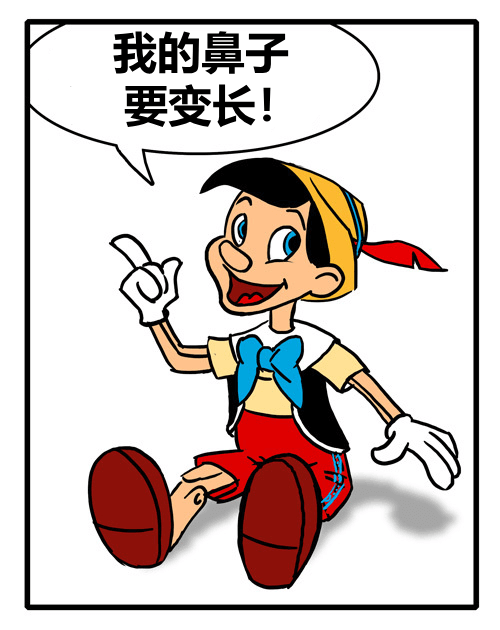
\includegraphics[scale=0.4]{figure/pinocchio.png}
\end{center}

这种现象的一个更奇怪的例子是\emph{奎因悖论(Quine's Paradox)}:
\begin{center}
    \textcolor{red}{``Yields falsehood when preceded by its quotation'' \\yields falsehood when preceded by its quotation.}
\end{center}
这个问题留给你自己思考。我只想说,像这样自相矛盾的说法实在是太病态了,以至于我们不必考虑它们。这就是为什么我们的定义禁止了它们。

\subsection{变量命题}

另一类非数学陈述涉及\textbf{未量化变量}。例如,拿这句话来说:
\begin{center}
    ``\textcolor{red}{$x^2 - 1 = 0$}''
\end{center}
这在语法上当然是正确的,我们也能理解它,但它的真值是什么呢?我们不知道!如果 $x = 1$,则该句话为\verb|真|,但如果 $x = 8$,则为\verb|假|,如果 $x = \mathbb{N}$ 或 $x = \text{于儿}$,则该句话没有意义!因此,我们也希望禁止这样的语句。不过,这些类型的语句非常有用且常见。我们将它们称为\textbf{变量命题},因为它们提出的主张\emph{依赖于}某些变量。

对于上面的语句,我们可以将 $P(x)$ 定义为变量命题 ``$x^2 - 1 = 0$''。我们通常会将此声明写为
\begin{center}
    \textcolor{olivegreen}{令 $P(x)$ 为陈述 ``$x^2 - 1 = 0$''。}
\end{center}
通常用大写字母表示变量命题和数学陈述,用小写字母表示其中包含的变量。(但这不是一个要求,只是一种常见的约定。)

现在定义了这个变量命题,我们可以通过将特定值\emph{分配}给表达式中的变量 $x$ 来创建正确的数学陈述。我们可以说 $P(1)$ 为\verb|真|而 $P(0)$ 为\verb|假|。我们还可以对 $P(x)$ 进行\textbf{量化}。例如,下面语句是一个为\verb|真|的数学陈述:
\begin{center}
    存在 $x \in \mathbb{R}$ 使得命题 $P(x)$ 为\verb|真|。
\end{center}
而下面语句是一个为\verb|假|的数学陈述:
\begin{center}
    对于每个 $x \in \mathbb{R}$,命题 $P(x)$ 为\verb|真|。
\end{center}
想想为什么这些陈述具有我们所说的真值。你能明白为什么它们是数学陈述吗?你将如何证明这些说法?

\subsubsection*{定义变量命题}

请注意我们用来定义变量命题的格式,如上面的格式:
\begin{enumerate}[label=(\arabic*)]
    \item 我们给命题起一个字母名称(如 $P$);
    \item 我们表明它对一些变量的依赖性,每个变量都有一个字母名称(如 $x$ 和 $y$);
    \item 我们在实际命题本身周围加上引号;
    \item 我们不包含任何在命题上下文中没有意义的新字母。
\end{enumerate}

这种格式经过精心选择,因为它精确且明确。它为命题中的每个字母赋予含义,并清楚地区分命题中的内容和不包含的内容。

例如,以下是变量命题的\textcolor{red}{\textbf{糟糕}}``定义''。我们会指出为什么它们不好的理由,并给出进行适当修正的建议。
\begin{itemize}
    \item \textcolor{red}{令 $Q(y)$ 为命题``$x < 0$''。}\\
        \textbf{原因}:$x$ 是什么?$y$ 在哪里?我们不知道命题上下文中的 $x$ 是什么,所以这是一个糟糕的定义。\\
        修改为:
        \begin{center}
            \textcolor{olivegreen}{令 $Q(x)$ 为陈述 ``$x<0$''。}
        \end{center}
        就完美了。括号内的变量是后面引号中陈述使用的变量。太棒了。
    \item \textcolor{red}{对于每个 $x \in \mathbb{R}$,令 $P(x)$ 为命题 $x^2 \ge 0$。}\\
        \textbf{原因}:这句话的作者是否想断言无论 $x \in \mathbb{R}$ 是什么 $x^2 \ge 0$? ``对于每个 $x \in \mathbb{R}$'' 这句话是否意味着是命题的一部分?\\
        如果我们将其解释为 $P(x)$ 被定义为 ``$x^2 \ge 0$'',并且这个定义是针对每个 $x \in \mathbb{R}$ 进行的,那么……好吧,这可能是合理的。\\
        然而,如果我们将其解释为 $P(x)$ 被定义为 ``对于每个 $x \in \mathbb{R}$, $x^2 \ge 0$'',那么……嗯,这肯定是不同的。事实上,这甚至不是一个正确定义的命题!命题 $P(x)$ 应取决于输入值 $x$,但不应允许更改或进一步量化命题内的变量!\\
        这个命题最初的写法有两种可能的解释,而且它们非常不同。因此,这是一个糟糕的定义。\\
        如果我们修改为:
        \begin{center}
            \textcolor{olivegreen}{对于每一个 $x \in \mathbb{R}$,定义 $P(x)$ 为陈述 ``$x^2 \ge 0$''。}
        \end{center}
        就会好很多。正如我们下面提到的,从技术上讲,我们不必告诉读者我们想要定义命题的 $x$ 值。不过,也许这只是一些有用的信息,所以写出来并没有什么坏处。
    \item \textcolor{red}{令 $T(x, y)$ = ``$x^2 - 7 = y$''。}\\
        \textbf{原因}:在这种情况下 ``$=$'' 是什么意思?当我们希望比较两个数字并说它们的值相等(或两个集合并说它们的元素相等)时,该符号才适用。对象 $T(x, y)$ 是一个数学陈述,要么为\verb|真|,要么为\verb|假|。因此,它没有数值可以与其他任何东西进行比较。\\
        同理,给定 $x$ 和 $y$ 的值,语句 ``$x2 - 7 = y$'' 要么为\verb|真|,要么为\verb|假|,因此说该方程``等于''其他值是没有意义的。它具有真值,而不是数值。\\
        如果我们改为:
        \begin{center}
            \textcolor{olivegreen}{令 $T(x, y)$ 为 ``$x^2 - 7 = y$''。}
        \end{center}
        那就完美了。
\end{itemize}

我们已经做了足够多的错误示范了,不想把任何不好的想法灌输给你,真的!然而,根据过去的经验,我们知道这些是学生书写命题时常犯的错误(要么是无意的,要么没有意识到为什么他们是错的),所以我们觉得有必要分享出来。

关于变量命题最后有一点说明。定义命题时不必说明变量从何而来。可以稍后在调用命题时或者使用变量的特定值时填写。也就是说,我们可以定义
\begin{center}
    令 $T(x, y)$ 为 ``$x^2 - 7 = y$''。
\end{center}
而无需指定 $x$ 和 $y$ 到底是自然数、整数、复数还是其他类似数字。稍后,我们可以说 $T(3, 2)$ 为\verb|真|,$T(\pi, -1)$ 为\verb|假|,并且 $T(\varnothing, \mathbb{N})$ 没有意义,但在定义 $T(x, y)$ 时,我们不需要以某种方式预期任何这些解释。

\subsection{词序至关重要!}\label{sec:section4.2.4}

我们将在下一节中详细讨论\textbf{量化}变量的概念。现在,我们想考虑一个更加引人注目的数学陈述示例,它说明了语句中词序的重要性。分析如下语句的结构也将是下一节的主要目标。
\begin{center}
    存在一个实数 $y$,使得对于每个实数 $x$, $y = x^3$。
\end{center}
这个句话说了什么?它说的是无论 $x \in \mathbb{R}$ 是什么,我们都可以找到一个数字 $y \in \mathbb{R}$ 使得 $y = x^3$ 为\verb|真|。这是荒唐的!怎么可能有一个数字是所有数字的立方呢?这句话确实是一个数学陈述,但它绝对为\verb|假|。但下面的说法又如何呢?
\begin{center}
    对于每个实数 $x$,存在一个实数 $y$,使得 $y = x^3$。
\end{center}
上面这句话为\verb|真|!你看出两个句子之间的区别了吗?它们包含完全相同的单词和符号,但顺序不同。前一句断言存在某个数字是每个实数的立方(此为\verb|假|),而后一句断言每个实数都有一个立方根,此为\verb|真|。这个例子强调了词序的重要性。

\subsection{习题}

\subsubsection*{温故知新}

以口头或书面的形式简要回答以下问题。这些问题全都基于你刚刚阅读的内容,所以如果忘记了具体的定义、概念或示例,可以回去重读相关部分。确保在继续学习之前能够自信地回答这些问题,这将有助于你的理解和记忆!

\begin{enumerate}[label=(\arabic*)]
    \item 数学陈述的重要定义属性是什么?
    \item 数学陈述和变量命题有什么区别?
    \item 为什么哥德巴赫猜想是一个数学陈述?
    \item 以下定义变量命题的尝试有什么问题?
        \begin{center}
            \textcolor{red}{令 $Q(x, y, z)$ 为 $7x - 5y + z$}
        \end{center}
\end{enumerate}

\subsubsection*{小试牛刀}

尝试回答以下问题。这些题目要求你实际动笔写下答案,或(对朋友/同学)口头陈述答案。目的是帮助你练习使用新的概念、定义和符号。题目都比较简单,确保能够解决这些问题将对你大有帮助!

\begin{enumerate}[label=(\arabic*)]
    \item 对于以下每个语句,判断它是否是数学陈述。如果是,请判断它为\verb|真|还是为\verb|假|。如果不是,请解释原因。
        \begin{enumerate}[label=(\alph*)]
            \item $142857 \cdot 5 = 714285$
            \item 对于每个 $n \in \mathbb{N}$, $\displaystyle{\sum_{k \in [n]}k=\frac{n(n+1)}{2}}$。
            \item 对于任何集合 $A$ 和 $B$,如果 $A \subseteq B$,则 $B \subseteq A$。
            \item 对于任何集合 $A$ 和 $B$,如果 $A \subseteq B$,则 $\mathcal{P}(A) \subseteq \mathcal{P}(B)$。
            \item 数学就是酷。
            \item $1 + 2 = 0$
            \item 对于任意 $x, y \in \mathbb{Z}$,如果 $x \cdot y$ 为偶数,则 $x$ 和 $y$ 都为偶数。
            \item 对于任何 $x, y \in \mathbb{Z}$,如果 $x$ 和 $y$ 都为偶数,则 $x \cdot y$ 也为偶数。
            \item $1+ = 2$
            \item $-5 + \mathbb{Z} \ge \pi$
            \item $x = 7$
            \item 这句话不正确。
        \end{enumerate}
    \item 回顾前三章,找出数学陈述的一些例子和伪例。\\
    你能找到变量命题吗?它们是按照我们在本节中指定的方式编写的吗?你能修改它们使得它们正确书写吗?
    \item 写出一个变量命题的正确定义,当两个输入值具有非负和时,该命题为真。\\
    然后,找到命题为\verb|真|和为\verb|假|时的两个实例。
    \item 令 $S$ 为集合 $\{1, 2, 3, 6, 8, 10\}$。
        \begin{enumerate}[label=(\alph*)]
            \item 编写一个变量命题的正确定义,输入两个变量并判断它们的差的绝对值是否是 $S$ 的元素。然后,分别找到命题为\verb|真|和为\verb|假|时的两个实例。
            \item 编写一个变量命题的正确定义,输入两个集合并确定它们的交集是否是 $S$ 的子集。然后,分别找到命题为\verb|真|和为\verb|假|时的两个实例。
        \end{enumerate}
        (注意:给定任意集合 $X$ 和任意对象 $x$,它必须是 $x \in X$ 或 $x \notin X$。)
    \item 想出另一个数学命题,它为\verb|真|,但当我们交换一些单词的顺序时,它就变为\verb|假|。(请参阅最后一小节中的示例以获得一些灵感。)
    \item 对于以下定义变量命题,请确定它们是否正确。注意:这并不意味着判断它为\verb|真|还是为\verb|假|;相反,我们想知道该声明是否写得好且合理。\\
    如果由于某种原因写得不正确,请解释错误原因并编写一条新陈述来修复该错误。
    \begin{enumerate}[label=(\alph*)]
        \item 令 $P(x)$ 为 ``$x > 1$''。
        \item 令 $Q(x)$ 为命题 ``$x^2 - 1 > 0$''。
        \item 对于每个 $a,b \in \mathbb{R}$,令 $R(a, b)$ 为 ``$a^3 = b$''。
        \item 令 $P(x)$ 为 $x > 1$。
        \item 令 $T(z) = $ ``$z$ 为质数''。
        \item 对于每个 $x \in \mathbb{R}$,令 $Q(x)$ 为命题 ``$x^2 - 1 > 0$''。
        \item 对于每个 $x \in \mathbb{R}$,令 $Q(x)$ 为 ``$x^2 - 1 > 0$''。
        \item 令 $S(a)$ 为 ``$b^2 > 4$''。
        \item 对于每个 $x \in \mathbb{R}$,令 $Q(x)$ 为 $x^2 - 1 > 0$。
    \end{enumerate}
\end{enumerate}

\newpage
% !TeX root = ../../book.tex
\section{量词:存在量词和全称量词}

现在,我们将介绍一些方便的符号,使我们能够缩短迄今为止看到的一些语句,并用数学符号表达冗长的、基于语言的短语。这些符号的另一个好处是我们能够更轻松地表达和分析数学陈述。具体来说,我们现在介绍符号 ``$\forall$'' 和 ``$\exists$''。

\begin{definition}
    符号 ``$\forall$'' 代表短语 ``\dotuline{对于所有}''。

    符号 ``$\exists$'' 代表短语 ``\dotuline{存在}''。

    我们称 ``$\forall$'' 为全称量词,称 ``$\exists$'' 为存在量词。

    以 ``$\forall$'' 开头的数学陈述被称为``全称量化'',以 ``$\exists$'' 开头的数学陈述被称为``存在量化''。
\end{definition}

\subsection{用法和符号}

可以用 ``$\forall$'' 替换的其他常见短语还有``对于每个''、``对于任意''、``每当''、``给定任何''甚至``如果''。

可以用 ``$\exists$'' 替换的其他常见短语还有``对于某个''、``至少有一个''、``有''甚至``某个''。\\

\begin{example}
    让我们先来看几个简单的例子,以开始我们的实践。以下每种情况,我们都希望使用这些符号来表达数学思想,或者尝试以更``罗嗦''的方式解释量化陈述。
    \begin{itemize}
        \item ``每个实数的平方都是非负数。''
            这是一个简单直白的陈述,事实上,这个陈述为\verb|真|。我们可以将其写为:
            \[\forall x \in \mathbb{R} \centerdot x^2 \ge 0\]
            ``大点'' 将陈述的量化部分与关于变量 $x$ 的声明(在量化中引入)分开。\\
            另一种写法是:
            \begin{center}
                定义 $S(x)$ 为 ``$x^2 \ge 0$''。那么命题就是:$\forall x \in \mathbb{R} \centerdot S(x)$。
            \end{center}
        \item ``存在 $\mathbb{N}$ 的一个子集以 $7$ 作为元素。''
            这是一个\emph{存在}声明。它断言我们可以找到具有特定属性的对象。我们将其写为:
            \[\exists S \in \mathcal{P}(\mathbb{N}) \centerdot 7 \in S\]
            请记住,$\mathcal{P}(\mathbb{N})$ 是 $\mathbb{N}$ 的\emph{幂集},即 $\mathbb{N}$ 的所有子集的集合;因此,根据要求,$S \in \mathcal{P}(\mathbb{N})$ 意味着 $S \subseteq \mathbb{N}$。
        \item ``每个整数都有一个\emph{加法逆元}(即,当与原始数字相加时,结果为 $0$)。''
            ``加法逆元''的概念是一个通用概念,适用于一些称为\emph{环}和\emph{域}的数学对象。我们不会在本书中讨论这些对象,但你会在抽象代数课程中接触它们。\\
            我们可以将此声明写为:
            \[\forall a \in \mathbb{Z} \centerdot \exists b \in \mathbb{Z} \centerdot a + b = 0\]
            读作:
            \begin{center}
                对于任意整数 $a$,都存在一个整数 $b$,使得 $a + b = 0$。
            \end{center}
            或
            \begin{center}
                无论给定什么整数 $a$,我们都可以找到一个具有 $a + b = 0$ 性质的整数 $b$。
            \end{center}
            同样,我们可以通过将 $I(a, b)$ 定义为 ``$a + b = 0$'' 来稍微缩短符号,然后将声明写为:
            \[\forall \in \mathbb{Z} \centerdot \exists b \in \mathbb{Z} \centerdot I(a, b)\]
    \end{itemize}
\end{example}

\begin{example}
    以下是正确使用 ``$\forall$'' 的一些示例,以及如何使用该符号的一些等效表述。
    \begin{itemize}
        \item $\forall x \in \mathbb{R} \centerdot x^2 \ge 0$
        \item 对于所有实数 $x$,我们有 $x^2 \ge 0$。
        \item 每个实数 $x$ 都满足 $x^2 \ge 0$。
        \item 当 $x$ 为实数时,我们知道 $x^2 \ge 0$。
    \end{itemize}
    同样,下面是符号 ``$\exists$'' 的正确用法和等效表述的示例。
    \begin{itemize}
        \item $\exists x \in \mathbb{R} \centerdot x^2 - 4x + 4 = 0$
        \item 存在实数 $x$ 使得 $x^2 - 4x + 4 = 0$。
        \item 存在实数 $x$ 满足 $x^2 - 4x + 4 = 0$。
        \item 某个实数 $x$ 具有 $x^2 - 4x + 4 = 0$ 的性质。
    \end{itemize}
\end{example}

\subsubsection*{朗读量化陈述}

\begin{example}
    现在来看一些更难的例子。让我们回顾一下我们在上一节末尾写的短语,并使用这个新的符号来表达它们。考虑一下这个陈述:
    \begin{center}
        对于每个实数 $x$,存在一个实数 $y$,使得 $y = x^3$。
    \end{center}
    为了以符号形式表达这一点,我们将 $P(x, y)$ 定义为命题 ``$y = x^3$'',然后将该陈述写为:
    \[\exists y \in \mathbb{R} \centerdot \forall x \in \mathbb{R} \centerdot P(x, y)\]
    从逻辑上讲,这是正确的,并且相当简洁。目前,我们有时会使用一些``辅助短语''来重写该陈述,以帮助我们更好地阅读出来。特别是,我们在朗读时会使用这些``辅助短语'',因此我们将它们写下来,为你提供一些口头解释逻辑符号的额外练习。我们将上面的陈述朗读为
    \begin{center}
        存在一个实数 $y$,使得对于每个实数 $x$,陈述 $P(x, y)$ 成立。
    \end{center}
    短语``使得''就是一个``辅助短语'',它将存在量化与短语的其余部分联系起来。下一小节包含有关何时以及如何使用此辅助短语的一些重要信息!
\end{example}

上述陈述的量化部分之间的``大点''只是用于分隔陈述的各个部分,使其更易于阅读。它对应于说话中的停顿或休止,就像逗号一样,但有时它具有语音含义(例如 ``$\exists y \in \mathbb{R}$'' 部分后面的``使得'')。

不过,我们不想使用逗号,因为我们已经将它们用于其他含义。例如,
\[x, y \in S\]
表示 ``$x$ 和 $y$ 都是集合 $S$ 的元素''。``大点''是不同的符号。

相对而言,由于我们的数学生涯还很年轻,因此我们鼓励你尽量写下``使得''和``为\verb|真|''等辅助短语来指导你的理解。这会提醒你句子的含义,并帮助你练习以简洁的形式阅读和书写此类陈述。请记住,你在学习一门语言,你需要练习将句子从你知道的一种语言(汉语)\emph{翻译}成另一种语言(数学)。例如,你可能想将上面例子写为(或者,至少在你的脑海里读作):
\[\exists y \in \mathbb{R} \;\text{使得}\; \forall x \in \mathbb{R} \centerdot P(x, y) \;\text{为}\verb|真|\]
(顺带一提,当在白板/黑板或纸上书写时,通常会用 ``s.t.'' 代替 ``such that'' 或``使得'',以节省书写时间。这只是表明 ``such that'' 或``使得''这个短语在数学写作中是多么普遍;我们已经有了一个约定的缩写了!)

\subsection{短语``使得''以及量词的顺序}

请注意,辅助短语``使得''总是跟在\emph{存在}量化之后,并且\emph{只能}跟在存在量化之后。这是因为带有 ``$\exists$'' 的声明断言了具有某种属性的对象的存在,而陈述的其余部分是对该特殊属性的描述。因此,这里用``使得''是有合理的,可以帮助我们正确阅读句子。考虑下面这个数学陈述:
\[\exists y \in \mathbb{R} \centerdot \forall x \in \mathbb{R} \centerdot P(x, y)\]
如果我们朗读上面的陈述,但把``使得''这个短语放错了地方,把它放在 ``$\forall$'' 后面而不是 ``$\exists$'' 后面,会发生什么?这会产生这样一句话:
\begin{center}
    \textcolor{red}{$\exists y \in \mathbb{R} \quad \forall x \in \mathbb{R}$ 使得 $P(x, y)$ 为真}
\end{center}
我们前面分析过这可以用两种方式解释,但这两种方式\emph{都不是}真正正确的含义,这就是我们用\textcolor{red}{红色}书写的原因!

一方面,有人可能会说这样的句子根本不符合语法,也没有任何意义,因为 ``使得'' 不属于\emph{全称}量化。这相当于举手说:``我不知道你的意思!''

另一方面,人们可能会稍微解读一下这句话,并认为作者真正的意思是
\[\exists y \in \mathbb{R}, \forall x \in \mathbb{R}, \;\text{使得}\; P(x, y) \;\text{为}\verb|真|\]
或用语言表达
\begin{center}
    对于每个 $y \in \mathbb{R}$,存在 $x \in \mathbb{R}$,使得 $P(x, y)$ 为\verb|真|。
\end{center}
这里,逗号表示短语顺序的倒置,这在英语中很常见。(例如,考虑以下句子:``我笑了 \emph{30 Rock} 的每一集,全心全意地。''这与说``我全心全意地笑了 \emph{30 Rock} 的每一集。'')这句话是等效的,那么, 写作
\[\exists y \in \mathbb{R} \centerdot \forall x \in \mathbb{R}, \;\text{使得}\; P(x, y) \;\text{为}\verb|真|\]
这与我们考虑的原始数学陈述不同,事实上,它实际上是我们在上一节中看到的另一个陈述(参见第 \ref{sec:section4.2.4} 节),它是错误的!回想一下 \ref{sec:section4.2.4} 节中的类似陈述,只是语序颠倒了:
\begin{center}
    存在一个实数 $x$,对于每个实数 $y$,我们有 $y = x^3$。
\end{center}
我们可以用符号将其表示为
\[\exists x \in \mathbb{R} \centerdot \forall y \in \mathbb{R} \;\text{使得}\; P(x, y) \;\text{为}\verb|真|\]
看呐!短语``使得''放置错位置导致对句子的合理语言解释与最初的含义完全相反。哎呀!这就是为什么我们必须\emph{始终且仅在}\textbf{存在量化}之后小心使用``使得''。请记住,我们不会总是写出辅助短语,因此当你在脑海中朗读陈述或读给他人听时,必须谨记正确使用它,以确保获得正确的、预期的解释。

上一节中这个例子的目的是指出词序的重要性。现在我们有了符号来代替这些单词和短语,我们想强调这些符号的顺序也十分重要。我们上面看到的两个数学陈述包含完全相同的单词和符号,但顺序不同,一个为\verb|假|,另一个为\verb|真|。可见,顺序是极其重要的!

\subsection{``固定''变量和依赖}\label{sec:section4.3.3}

当我们讨论量词顺序的主题时,我们还要提到以下示例来强调量词的顺序决定何时将变量视为表达式中的\textbf{固定变量}。

考虑一下这句话:``任何大于或等于 $4$ 的偶数都可以写成两个质数之和。''(回想一下,这是我们上一节中讨论过的著名的\textbf{哥德巴赫猜想}。)为了从逻辑上和符号上表达这个陈述,我们可以写成
\begin{align*}
    &\text{令} X \text{为除} 2 \text{以外的偶数的集合。}\\
    &\text{设} P \text{为质数集。}\\
    &\text{定义} Q(n, a, b) \text{为``}n = a + b\text{''。}\\
    &\text{那么声明就是:}
\end{align*}
\[\forall n \in X \centerdot \exists a, b \in P \centerdot Q(n, a, b)\]

请注意,我们在这里使用了一些简写。像``$\exists a, b \in P$'' 这样的短语完全可以表达上述陈述,而不必写成
\[\forall n \in X \centerdot \exists a \in P \centerdot \exists b \in P \centerdot Q(n, a, b)\]
当两个变量被量化为同一集合中的元素,并且两个紧挨着时,将它们组合成一个量化是很常见的。我们甚至可能会看到这样的数学陈述,
\[\forall x, y \in \mathbb{Z} \centerdot \exists a, b, c, d \in \mathbb{Z} \centerdot a + b + c + d = x + y \;\text{且}\; a + b \ne x \;\text{且}\; c + d \ne y\]
(顺便问一下,这个陈述断言了什么?它为\verb|真|还是为\verb|假|?它取决于 $\mathbb{Z}$ 的上下文吗?如果我们将两处都换成 $\mathbb{N}$ 或 $\mathbb{R}$ 会怎样?)

\subsubsection*{量化``固定''变量}

回顾上面的例子,我们定义了 $Q(n, a, b)$。我们提出这个例子的原因是为了指出初始量化 ``$\forall n \in X$'' 用于\emph{固定} $n$ 的特定值,该值将用于陈述的其余部分。之后,断言 ``$\exists a, b \in P$'' 及其后续属性 $Q(n, a, b)$ 取决于 $n$ 的\emph{固定}但\emph{任意}值。

整个陈述说的是,无论选择什么样的 $n$,我们都可以找到满足属性 $Q$ 的值 $a, b$。(当然,请注意,$a, b$ 的这些值可能\emph{取决于} $n$。)但是,量化顺序告诉我们这些值 $a, b$ 可能\emph{取决于}所选的 $n$。这就是我们要强调的。

作为示例,考虑语句中变量 $n$ 的特定值。我们知道 $8 \in X$ 因为 $8$ 是偶数且 $8 \ge 4$。当 $n = 8$ 时会发生什么?你能找到 $a, b \in P$ 使得 $a + b = 8$ 吗?当然可以,我们可以让 $a = 3$ 且 $b = 5$。那么当 $n = 14$ 时呢?你能找到满足 $a+b = 14$ 的 $a, b \in P$ 吗?当然可以,你现在的选择必然与以前的\emph{不同}。这就是我们所说的 $a$ 和 $b$ \emph{依赖于} $n$ 的意思。(顺便问一下,在 $n = 14$ 时,你能找到 $a$ 和 $b$ 吗?我们可以想出几个可行的选择!)

为了确保你充分理解这部分讨论的内容,请考虑以下问题并回答:上面的陈述和下面的陈述有何区别?
\[\exists n \in X \centerdot \exists a, b \in P \centerdot Q(n, a, b)\]
这个陈述为\verb|真|还是为\verb|假|?为什么?

\subsection{指定量化集}

关于量词还有一点我们需要强调,每当使用量词时,我们都必须指定一个集合。下面这句话
\[\forall x \centerdot x^2 \ge 0\]
可能``看上去为\verb|真|'',但实际上\textbf{毫无意义}。$x$ 是什么?它从何而来?``对于每一个 $x$ …… ''从哪里获取?如果 $x$ 不是数字怎么办?

我们需要指定对象 $x$ ``来自''哪里,以便我们知道 $x^2 \ge 0$ 是否是一个明确定义、符合语法的短语,更不用说它是否为\verb|真|。如果我们将句子修改为
\[\forall x \in \mathbb{R} \centerdot x^2 \ge 0\]
那么这就是一个定义明确、符合语法(并且正确!)的数学陈述。但是,如果我们将句子修改为
\[\forall x \in \mathbb{C} \centerdot x^2 \ge 0\]
那么这就是一个定义明确但错误的数学陈述!这是因为 $i \in \mathbb{C}$ 但 $i^2 = -1 < 0$。(请记住,本书中我们不会大量使用复数 $\mathbb{C}$ 的集合,但它提供了一些有趣且具有启发性的示例,就像上面这个。)

这里的主要教训是\textbf{上下文}确实很重要。它可以改变陈述的含义及其真值。因此,我们必须始终确保指定一个从中提取变量值的集合。

\subsubsection*{一个例外}

打脸来得好快,我们不得不承认``永远指定量化集''这一规则有一个例外,但这个例外是有充分理由的。考虑以下声明:
\begin{center}
    对于任意集合 $A, B,C$,等式 $(A \cup B) \cap C = (A \cap C) \cup (A \cap B)$ 成立。
\end{center}
这个数学陈述为\verb|真|。(你能证明这一点吗?尝试使用双重包含论证!)

我们如何以符号形式写出这个陈述呢?这是一个\emph{全称}量化(``对于任意……''),因此我们需要使用 ``$\forall$'' 符号。这里的变量(用 $A,B,C$ 表示)是\emph{集合}。他们来自哪里?我们将从什么集合中提取它们?

我们非常确定你想说``所有集合的集合''。但这存在一个大问题!还记得我们在上一章讨论的罗素悖论吗?(请参阅第 \ref{sec:section3.3.5} 节。)所有可能集合的集合本身并\emph{不是}一个集合!因此,我们不能将这个陈述符号化地写成
\[\forall A, B,C \in \underline{\qquad} \centerdot (A \cup B) \cap C = (A \cap C) \cup (A \cap B)\]
因为我们不知道如何用\emph{集合}来填补空白。

由于这个问题,我们将继续使用``对于任意集合 $A,B,C$ ……''之类的短语,而不是用符号形式表达。当我们自己做笔记或在草稿纸上解题时,可以随意写下 ``$\forall A,B,C$'',并且知道它其实代表了集合的量化。然而,当更正式地书写时(例如,书面作业),你应该坚持使用上面的措辞。

\subsection{习题}

\subsubsection*{温故知新}

以口头或书面的形式简要回答以下问题。这些问题全都基于你刚刚阅读的内容,所以如果忘记了具体的定义、概念或示例,可以回去重读相关部分。确保在继续学习之前能够自信地回答这些问题,这将有助于你的理解和记忆!

\begin{enumerate}[label=(\arabic*)]
    \item $\forall$ 和 $\exists$ 和有什么不一样?
    \item 如何朗读下面的陈述?
        \[\forall x \in \mathbb{R} \centerdot \exists y \in \mathbb{R} \centerdot x = y^3\]
    \item 下面的语句为什么不是正确的数学陈述?
        \[\exists y \centerdot y + 3 > 10\]
        以下两个陈述之间有何区别(如果有的话)?
        \[\exists x \in \mathbb{N} \centerdot ∃y \in \mathbb{N} \centerdot x + y = 5\]
        \[\exists x, y \in \mathbb{N} \centerdot x + y = 5\]
        它们为\verb|真|还是为\verb|假|?
    \item 以下两个陈述之间有何区别(如果有的话)?
        \[\exists a, b \in \mathbb{Z} \centerdot a \cdot b = -3\]
        \[\exists \heartsuit, \diamondsuit \in \mathbb{Z} \centerdot \heartsuit \cdot \diamondsuit = -3\]
        它们为\verb|真|还是为\verb|假|?
    \item 为什么下列语句不是正确的量化陈述?
        \textcolor{red}{\begin{itemize}
            \item $\exists x \centerdot x > 7$
            \item $\forall y \in \mathbb{Z}$
            \item $\forall z > 2 \centerdot z^2 > 4$
            \item $\forall w \in \mathbb{Z} \centerdot w^2 = t \centerdot \exists t \in \mathbb{N}$
        \end{itemize}}
\end{enumerate}

\subsubsection*{小试牛刀}

尝试回答以下问题。这些题目要求你实际动笔写下答案,或(对朋友/同学)口头陈述答案。目的是帮助你练习使用新的概念、定义和符号。题目都比较简单,确保能够解决这些问题将对你大有帮助!

\begin{enumerate}[label=(\arabic*)]
    \item 回顾 \ref{sec:section4.3.3} 节,我们用符号表示法表达了哥德巴赫猜想。我们将 $X$ 定义为除 $2$ 之外的所有偶数的集合。用符号、量词和集合构建符(也许还有集合运算,具体取决于你的操作方式)编写 $X$ 的定义。
    \item 写一个以量词开头的数学陈述的示例,如果该量词是 ``$\exists$'',则该陈述为\verb|真|,但如果该量词为  ``$\forall$'',则该陈述为\verb|假|。
    \item 写一个变量命题 $P(x)$ 的例子,使得
        \[\forall x \in \mathbb{N} \centerdot P(x)\]
        为\verb|真|,但
        \[\forall x \in \mathbb{Z} \centerdot P(x)\]
        为\verb|假|。
    \item 对于以下每个数学陈述,使用量词将其写成符号形式。(首先确保正确定义可能需要的任何变量命题!)然后,确定该陈述为\verb|真|还是为\verb|假|。
        \begin{enumerate}[label=(\alph*)]
            \item 存在一个严格大于每个整数的实数。
            \item 每个整数都具有其平方小于或等于其立方的性质。
            \item 每个自然数的平方根都是实数。
            \item $\mathbb{N}$ 的每个子集都以数字 $3$ 作为元素。
        \end{enumerate} 
    \item 阅读以下每个量化陈述的符号表示并朗读出来。然后,确定该陈述为\verb|真|还是为\verb|假|。
        \begin{enumerate}[label=(\alph*)]
            \item $\forall x \in \mathbb{N} \centerdot \exists y \in \mathbb{Z} \centerdot x + y < 0$
            \item $\exists x \in \mathbb{N} \centerdot \forall y \in \mathbb{Z} \centerdot x + y < 0$
            \item $\exists A \in \mathcal{P}(\mathbb{Z}) \centerdot \mathbb{N} \subset A \subset \mathbb{Z}$\\(回想一下,$⊂$ 的意思是``是……的真子集''。)
            \item 设 $P$ 为素数集。\\
                    $\forall x \in P \centerdot \exists t \in \mathbb{Z} \centerdot x = 2t + 1$
            \item $\forall a \in \mathbb{N} \centerdot \exists b \in \mathbb{Z} \centerdot \forall c \in \mathbb{N} \centerdot a + b < c$
            \item $\exists b \in \mathbb{Z} \centerdot \forall a, c \in \mathbb{N} \centerdot a + b < c$
        \end{enumerate} 
\end{enumerate}   

\newpage
% !TeX root = ../../book.tex
\section{量化陈述的逻辑否定}\label{sec:section4.4}

让我们回到之前使用过的示例陈述。定义 $P(x, y)$ 为 ``$y = x^3$'',然后定义 $Q_1$ 为陈述
\[\text{``}\exists y \in \mathbb{R} \centerdot \forall x \in \mathbb{R} \centerdot P(x, y)\text{''}\]
定义 $Q_2$ 为陈述
\[\text{``}\forall x \in \mathbb{R} \centerdot \exists y \in \mathbb{R} \centerdot P(x, y)\text{''}\]
请记住,$Q_1$ 为\verb|假|,$Q_2$ 为\verb|真|。

我们怎么知道 $Q_1$ 为\verb|假|?它表示存在某个具有特定属性的实数。要声明整个语句为\verb|假|,我们可能必须验证该属性并\emph{不}适用于\emph{每个}实数 $y$,但这需要很长时间!集合 $\mathbb{R}$ 无穷大!一种更有效的方法是证明该陈述的\textbf{否定}形式为\verb|真|。

我们所说的``否定''指的是\textbf{逻辑否},即在逻辑意义上与原始陈述``相反''的陈述。数学陈述的逻辑否具有与原始陈述相反的真值,因此,如果我们得到 $Q_1$ 的否定形式并证明它为\verb|真|,那么我们就证明了 $Q_1$ 本身为\verb|假|。

但是我们如何否定一个陈述呢?当我们注意到我们必须以某种方式证明关于\emph{每个}实数 $y$ 的某些事情时,我们已经有了正确的想法,因为原始陈述声称\emph{存在}。在本节中,我们将探讨如何正确地否定此类陈述。

我们应该注意到,到目前为止我们所讨论的内容背后有一些微妙但深刻的数学概念。为什么一个数学命题要么为\verb|真|,要么为\verb|假|呢?一个厚颜无耻(但完全正确)的回答是,``因为你把`\textbf{数学陈述}'定义为那样,傻逼!''是的,我们确实是这么做的,但我们\emph{为什么}要这么做呢?\verb|真|/\verb|假|二元性对数学为什么是\emph{有益的},或\emph{必要的}?这些都是有意义又难以回答的问题,绝对值得思考。对这些主题的讨论必然会深入研究数学哲学和人类思想,这当然是有趣且有价值的追求,但超出了本书/课程的范畴和目标。我们将依靠我们对真理的共同的、直觉的理解。

\subsection{否定全称量化}

全称声明(即 ``$\forall$'')的否定通常是一个存在声明(即``$\exists$''),反之亦然。在我们解决更大的否定任意量化陈述的问题之前,让我们看一个简单的例子。

假设 $S$ 为集合,$R(x)$ 是定义在每个 $x \in S$ 上的数学陈述。该陈述
\[\forall x \in S \centerdot R(x)\]
对集合 $S$ 中变量 $x$ 的每个可能值断言变量命题的真值。它表示,无论我们引用集合 $S$ 的哪个元素 $x$,我们都可以\emph{必然}得出命题 $R(x)$ 为\verb|真|。现在,如果这个陈述为\verb|假|,我们该如何\emph{证明}这一点呢?

如果每个元素 $x \in S$ 都满足某个属性为\verb|假|,则必定\emph{至少}有一个元素\emph{不}满足该属性。为了证明这一点,我们需要找到这样的元素;我们必须定义(或找到)一个元素 $x$ 并解释为什么 $R(x)$ 对于该特定元素不成立。(想想我们如何在语言上理解这个否定。我们在日常语言中一直这样做,甚至没有思考它。)那么,结论是,原始陈述的否定是
\[\exists x \in S \;\text{使得}\; R(x) \;\text{为假}\]

我们引入符号 $\neg$ 表示``\textbf{逻辑否}''或``\textbf{不}''。有了这个符号,我们就可以重写否定陈述
\[\neg\big(\forall x \in S \centerdot R(x)\big)\]
为
\[\exists x \in S \centerdot \neg R(x)\]
上面陈述的结论短语 $\neg R(x)$ 可以简化,具体取决于 $R(x)$ 是什么。例如,如果 $S = \mathbb{R}$ 且 $R(x)$ 为 ``$x^2 \ge 0$'',则否定陈述为
\[\text{``}\exists x \in \mathbb{R} \;\text{使得}\; x^2 < 0 \text{''}\]
因为 ``$x^2 < 0$'' 在逻辑上等价于 ``$\neg(x^2 \ge 0)$''。

但一般来说,我们必须将其保留为 ``$\neg R(x)$'',而不进一步深入命题 $R$。我们还将指出,一般来说,短语 ``$R(x)$ 为\verb|假|'' 和 ``$\neg R(x)$ 为\verb|真|'' 在逻辑上是等价的;他们都断言命题 $R(x)$ 不正确。

我们现在正在发展的这个概念就是\emph{反例}的含义,你以前可能听说过这个术语。为了\emph{反驳}全称量化陈述,我们必须证明存在量化陈述;该证明涉及显式定义集合中不满足指定属性的元素,这就是\textbf{反例}一词的由来。

\subsection{否定存在量化}

类似 
\[\exists x \in S \centerdot R(x)\] 
这样的陈述提出了存在性声明。它表示必须存在某个元素 $x$ 满足属性 $R(x)$。为了反驳这一主张,我们需要证明 $x$ 的任何值实际上都无法满足属性 $R$。因此,我们可以说陈述
\[\neg\big(\exists x \in S \centerdot R(x)\big)\]
在逻辑上等价于陈述 
\[\forall x \in S \centerdot \neg R(x)\]

如果我们考虑如何反驳这种存在性声明,就会发现这是合理的。假设你正在与某位朋友进行辩论,他告诉你某些 kwyjibo 具有它是 Zooqa 的属性。你会如何反驳他/她?你可能会说,``不对!给我任意你想要的 kwyjibo。我知道这不可能是 zooqa,原因如下……''然后你会解释为什么该属性无论如何都不成立。

现在,当你说``给我任意''时,你实际上是在执行全称量化!你是说,\emph{无论}你考虑哪种 kwyjibo,有些事情都是真的;也就是说,对于\emph{每个} kwyjibo,或 $\forall x \in K$(其中 $K$ 是所有 kwyjibo 的集合),某些事情为\verb|真|。

想一想并思考以下为什么我们发现/定义的逻辑否定是合理的。在本章后面,当我们考虑证明技术时,我们将解释考虑\emph{任意} kwyjibo 的策略以及为什么这实际上证明了我们上面刚刚写出的逻辑否定。眼下,我们希望你了解
\[\forall x \in S \centerdot \neg R(x)\] 
和
\[\exists x \in S \centerdot R(x)\]
具有相反的真值。

\subsection{一般量化陈述的否定}

到目前为止,我们所做的观察引出了否定量化陈述的一般方法。我们在第 \pageref{sec:section4.4} 页定义的陈述 $Q_1$ 的形式为
\[\exists y \in \mathbb{R} \centerdot C(y)\]
其中 $C(y)$ 是陈述的其余部分(当然,这\emph{取决于} $y$ 的值)。我们将 $C(y)$ 视为量化变量 $y$ 的某些\emph{属性};该属性内部可能有其他量词和变量,但从根本上讲,它只是断言 $y$ 的一些事实。

为了否定这一说法,我们按照上面讨论的方法写做
\[\forall y \in \mathbb{R} \centerdot \neg C(y)\]
现在,我们知道 $C(y)$ 本身就是一个全称量化陈述:
\[\forall x \in \mathbb{R} \centerdot y = x^3\]
我们也知道如何否定这种类型的陈述!其否定形式 $\neg C(y)$ 为
\[\exists x \in \mathbb{R} \centerdot y = x^3\]
这一步仅使用了我们上面看到的另一个否定方法。然后,把它们放在一起,我们可以说 $\neg Q_1$ 为陈述
\[\forall y \in \mathbb{R} \centerdot \exists x \in \mathbb{R} \centerdot y \ne x^3\]
我们可以\emph{证明}这个说法是正确的,从而证明原始陈述一定为\verb|假|。

(我们将此证明留作练习。提示:给定任意 $y \in \mathbb{R}$,定义一个 $x$ 值,该值将迫使 $y \ne x^3$ 为真。请注意,你对 $x$ 的选择取决于 $y$ 的值;它们是如何依赖的?)

看看这个否定是如何产生的:我们认识到原始陈述是一个\textbf{嵌套量词}序列(即连续几个量化变量的序列),末尾有一个变量命题,并且我们看到我们可以将量词序列的一部分视为它自身的陈述。然后,我们将否定从外部量词 ``传递到内部量词'',并将这些否定拼凑在一起。

遵循同样的想法,我们可以弄清楚如何识别具有较长量词序列的陈述。例如,看看下面这个陈述
\[\forall a \in A \centerdot \exists b \in B \centerdot \exists c \in C \centerdot \forall d, e \in D \centerdot Q(a, b, c, d, e)\]
要开始否定它,我们先从第一个量化处断开,并将其余部分视为其自身的命题 $R(a)$,并且它仅依赖于 $a$:
\[\forall a \in A \centerdot \big(\underbrace{\exists b \in B \centerdot \exists c \in C \centerdot \forall d, e \in D \centerdot Q(a, b, c, d, e)}_{R(a)}\big)\]
因此否定可以写成
\[\exists a \in A \centerdot \neg R(a)\]
但我们必须找出 $\neg R(a)$ 的另一种写法。我们需要重复上面的做法!只需将 ``$\exists b \in B$'' 与其余部分分开……接着你就知道是怎么回事了。尝试自己完成这些步骤,并确保最终得到以下结果,这就是原始陈述的逻辑否定:
\[\exists a \in A \centerdot \forall b \in B \centerdot \forall c \in C \centerdot \exists d, e \in D \centerdot \neg Q(a, b, c, d, e)\]

一般来说,我们可以这样说:要否定仅由量词和变量命题组成的命题,只需将每个 ``$\forall$'' 切换为 ``$\exists$'',反之亦然,即可否定命题。不要改变我们量化的任何集合,只改变量词本身和随后的命题;改变讨论范围是没有意义的。稍后,我们将了解如何否定其他类型的陈述,即由其他连词构建的更复杂的陈述。在此之前,我们需要继续定义和讨论其他连词。

\subsection{方法总结}

让我们总结一下本节的内容。
\begin{itemize}
    \item \textbf{否定全称量化:} \\
        设 $X$ 为集合,$P(x)$ 为命题。则全称量化的否定,
        \[\neg \big(\forall x \in X \centerdot P(x)\big)\]
        写为
        \[\exists x \in X \centerdot \neg P(x)\]
        用语言表达,我们已经证明了
        \begin{center}
            对于每个 $x \in X, P(x)$ 不都成立。
        \end{center}
        等价于
        \begin{center}
            存在元素 $x \in X$ 使得 $P(x)$ 不成立。
        \end{center}
    \item \textbf{否定存在量化:} \\
        设 $X$ 为集合,$Q(x)$ 为命题。则存在量化的否定,
        \[\neg \big(\exists x \in X \centerdot Q(x)\big)\]
        写为
        \[\forall x \in X \centerdot \neg Q(x)\]
        用语言表达,我们已经证明了
        \begin{center}
            不存在 $x \in X$ 使得 $Q(x)$ 成立。
        \end{center}
        等价于
        \begin{center}
            对于每个元素 $x \in X, Q(x)$ 都不成立。
        \end{center}
\end{itemize}

\subsubsection*{不要更改量化集!}

我们上面提到过,当否定一个陈述时,改变讨论范围是没有意义的。要思考为什么这是合理的,可以举一个现实生活中的例子。

假设我们说``这个书架上的每一本书都是用英语写的''。你如何证明我们在撒谎,我们的陈述实际上为\verb|假|?你必须在\emph{这个书架}上找出一本不是用英文编写的书。你不能从走廊那头的房间里拿一本法国小说说:``瞧,你错了!''这并不能证明我们的主张;因为讨论的领域不同,我们没有对其他房间书架上发生的事情做出任何声明。我们只是对这个\emph{特定}书架做出了断言。

同理,当否定陈述
\[\forall b \in T \centerdot P(b)\]
时,我们在不改变讨论领域(集合 $T$)的情况下得到
\[\exists b \in T \centerdot \neg P(b)\]
最初的声明仅断言了 $T$ 中元素的某些性质,因此它的否定也应仅断言这一点。

\subsection{排中律}

你知道吗?让我们实际讨论一下为什么我们可以谈论陈述及其\textbf{逻辑否定}。我们对\textbf{数学/逻辑陈述}的定义中包含这样一个想法:陈述的句子必须仅有一个真值,要么为\verb|真|,要么为\verb|假|。为什么我们可以这样做?在这里我们需要对定义负责!数学家必须为他们的系统设定基本规则 --- \textbf{公理},而我们希望我们的逻辑系统能够确保我们提出的每一个主张都是正确的或错误的,而不是两者兼有或二者皆无。

这种二元性确实是我们系统的\textbf{公理}。它在大多数数学中被广泛采用,被称为``\textbf{排中律}''。这个名字来源于这样一个想法,即每一个主张都要么为\verb|真|要么为\verb|假|,所以这两者之间没有\emph{中间立场};中间的部分被排除在外。

从本质上讲,这使得我们在数学方面的工作卓有成效:每个主张都有一个真值,而我们的目标就是找到该真值。有时,我们必须依靠这个公理,即我们商定的定律,来\emph{确保}某些主张要么为\verb|真|要么为\verb|假|,但不知道具体是哪个真值。下面是一个有趣且颇具代表性的例子。

\begin{proposition}
    存在实数 $a$ 和 $b$ 都为无理数,而 $a^b$ 为有理数。
\end{proposition}

(请记住,有理数是可以表示为整数相除形式的数,无理数是非有理数的实数。你能想到有理数和无理数的一些例子吗?)

\begin{proof}
    我们知道 $\sqrt{2}$ 为无理数。(问题:为什么?你能证明这一点吗?现在就试试。我们也将很快证明这一点!)

    $\sqrt{2}^{\sqrt{2}}$ 要么是有理数,要么是无理数。(这里使用了排中律。)让我们分别考虑这两种情况。
    \begin{itemize}
        \item 假设 $\sqrt{2}^{\sqrt{2}}$ 为有理数。那么令 $a=\sqrt{2}, b=\sqrt{2}$,$a, b$ 都是无理数,而 $a^b$ 为有理数。
        \item 假设 $\sqrt{2}^{\sqrt{2}}$ 为无理数。那么令 $a=\sqrt{2}^{\sqrt{2}}, b=\sqrt{2}$,$a, b$ 都是无理数,而
        \[a^b = \big(\sqrt{2}^{\sqrt{2}}\big)^{\sqrt{2}} = \sqrt{2}^{\sqrt{2} \cdot \sqrt{2}} = (\sqrt{2})^2 = 2\]
        为有理数。
    \end{itemize}
    无论哪种情况,我们都找到了实数 $a, b \in \mathbb{R}$,其中 $a$ 和 $b$ 都为无理数,而 $a^b$ 为有理数。这证明改命题为\verb|真|。
\end{proof}

这是一个\textbf{非构造性}证明的例子。它告诉我们某些东西存在(甚至将其缩小到两种可能性),但实际上并没有\emph{确切}告诉我们哪种可能性是我们要寻找的可能性。正是对排中律的直接运用才构成了这种情况。

(问题:你能证明 $\sqrt{2}^{\sqrt{2}}$ 是无理数吗?这是真的,但没有已知的``简单''方法来证明这一事实。也许你可以找到一个!)

本书中大多数证明都是\textbf{构造性}的(但不是全部)。也许你觉得这样很好,我们也倾向于觉得这样不错。如果我们声称某事物存在,我们应该能够向你\emph{展示}它,对吗?如果我们只是谈论\emph{为什么}某些这样的事物存在于某个地方,而无法指明它,你可能会相信我们,但你一定对此感觉不佳。因此,构造性证明\emph{在主观上会更好一些},我们将尽可能地采用构造性证明。但有时,构造性证明并不显而易见,我们不得不采用非构造性证明,就像我们在上面所做的那样。

\subsection{回顾:索引集运算与量词}

回顾一下第 \ref{sec:section3.6.2} 节,我们分别在定义 \ref{def:definition3.6.1} 和 \ref{def:definition3.6.2} 中定义了对索引集执行的集合操作(并集和交集)。主要思想是我们可以使用速记符一次性表达整个集合类的并集/交集。

仔细看看这些定义。例如,一个对象是否是索引并集的元素的特征是什么?该对象必须至少是并集中一个组成集合的元素。也就是说,需要存在某个以该对象为元素的集合。这听起来像是\emph{存在量化},不是吗?

同理,一个对象是否是索引交集的元素的特征是什么?该对象需要是所有组成集合的元素。也就是说,对于所有这些集合,该对象必须是其中的元素。这是一个\emph{全称量化}。

通过这些观察,我们可以使用新的量词符号重写索引集运算的定义:

\clearpage 

\begin{definition}
    假设 $I$ 为索引集,且对于某全集 $U$, $\forall i \in I, A_i \subseteq U$。则
    \[\bigcup_{i \in I} A_i = \{x \in U \mid \exists k \in I \centerdot x \in A_k\}\]
    \[\bigcap_{i \in I} A_i = \{x \in U \mid \forall i \in I \centerdot x \in A_i\}\]
\end{definition}

再次尝试做一下第 \ref{sec:section3.6.2} 节中的一些示例和练习。现在这些定义更有意义了吗?

\subsection{习题}

\subsubsection*{温故知新}

以口头或书面的形式简要回答以下问题。这些问题全都基于你刚刚阅读的内容,所以如果忘记了具体的定义、概念或示例,可以回去重读相关部分。确保在继续学习之前能够自信地回答这些问题,这将有助于你的理解和记忆!

\begin{enumerate}[label=(\arabic*)]
    \item 数学命题的\emph{否定}是什么?陈述及其否定是如何相关的?
    \item 为什么 $\forall$ 命题的否定是 $\exists$ 命题?\\
        为什么 $\exists$ 命题的否定是 $\forall$ 命题?
    \item 什么是非构造性证明?该术语适用于什么类型的主张($\exists$ 或 $\forall$)?
    \item 考虑声明
        \[\forall x \in S \centerdot P(x)\]
        为什么它的否定不是下面这两个?
        \textcolor{red}{
            \[\forall x \notin S \centerdot P(x)\]
            \[\exists x \notin S \centerdot \neg P(x)\]
        }
\end{enumerate}

\subsubsection*{小试牛刀}

尝试回答以下问题。这些题目要求你实际动笔写下答案,或(对朋友/同学)口头陈述答案。目的是帮助你练习使用新的概念、定义和符号。题目都比较简单,确保能够解决这些问题将对你大有帮助!

\begin{enumerate}[label=(\arabic*)]
    \item 对于以下每个陈述,写出其否定形式。哪一个 --- 原式形式还是否定形式 --- 为\verb|真|?
        \begin{enumerate}[label=(\alph*)]
            \item $\forall x \in \mathbb{R} \centerdot \exists n \in \mathbb{N} \centerdot n > x$
            \item $\exists n \in \mathbb{N} \centerdot \forall x \in \mathbb{R} \centerdot n > x$
            \item $\forall x \in \mathbb{R} \centerdot \exists y \in \mathbb{R} \centerdot y = x^3$
            \item $\exists y \in \mathbb{R} \centerdot \forall x \in \mathbb{R} \centerdot y = x^3$
        \end{enumerate}
    \item 对于以下每个陈述,写出其否定形式。哪一个 --- 原式形式还是否定形式 --- 为\verb|真|?
        \begin{enumerate}[label=(\alph*)]
            \item $\exists S \in \mathcal{P}(\mathbb{N}) \centerdot \forall x \in \mathbb{N} \centerdot x \in S$
            \item $\forall S \in \mathcal{P}(\mathbb{N}) \centerdot \exists x \in \mathbb{N} \centerdot x \in S$
            \item $\forall x \in \mathbb{N} \centerdot \exists S \in \mathcal{P}(\mathbb{N}) \centerdot x \in S$
            \item $\exists x \in \mathbb{N} \centerdot \forall S \in \mathcal{P}(\mathbb{N}) \centerdot x \in S$
        \end{enumerate}
    \item 设 $I = \{x \in \mathbb{R} \mid 0 < x < 1\}$。\\
        对于以下每个定义的集合,用量词写出确定数字 $y \in \mathbb{R}$ 是否为集合元素的定义条件。\\
        然后,确定集合是什么,并使用集合构建符写出答案。\\
        (并尝试使用双重包含论证来证明你的主张!)
        \begin{enumerate}[label=(\alph*)]
            \item $\displaystyle{S =\bigcup_{x \in I}\{y \in \mathbb{R} \mid x < y < 2\}}$
            \item $\displaystyle{T =\bigcap_{x \in I}\{y \in \mathbb{R} \mid -x < y < x\}}$
            \item $\displaystyle{V =\bigcup_{x \in I}\{y \in \mathbb{R} \mid -3x < y < 4x\}}$
        \end{enumerate}
    \item 令 $P = \{y \in \mathbb{R} \mid y > 0\}$。考虑下面这个声明:
        \[\forall \varepsilon \in P \centerdot \exists \delta \in P \centerdot \forall x \in \{y \in \mathbb{R} \mid -\delta < y < \delta\} \centerdot |x^3| < \varepsilon\]
        写出该命题的逻辑否定形式。\\
        这个陈述表达了什么?它的否定形式表达了什么?\\
        哪一个为\verb|真|?你能证明这一点吗?
    \item 设 $A,B,C,D$ 为任意集合。\\
        设 $P(x),Q(x, y),R(x, y, z)$ 为任意变量命题。\\
        写出下列各命题的否定形式。
        \begin{enumerate}[label=(\alph*)]
            \item $\forall a \in A \centerdot \exists b \in B \centerdot Q(a, b)$
            \item $\forall a \in A \centerdot \neg P(a)$
            \item $\forall c \in C \centerdot \forall d \in D \centerdot \neg Q(c, d)$
            \item $\forall a_1, a_2 \in A \centerdot \forall d \in D \centerdot R(a_1, a_2, d)$
            \item $\forall b_1, b_2, b_3 \in B \centerdot \neg R(b_1, b_2, b_3)$
            \item $\exists b \in B \centerdot \forall c \in C \centerdot \forall d \in D \centerdot R(d, b, c)$
        \end{enumerate}
\end{enumerate}

\newpage
% !TeX root = ../../book.tex
\section{逻辑连词}

为了从简单陈述(即仅由量词和命题组成的数学数学)构建复杂数学陈述,我们可以将多个陈述用某些单词和短语(例如``与''、``或''和``蕴涵'')连接起来,以创建更复杂的陈述并断言进一步的主张和真理。我们将这些单词和短语称为\textbf{逻辑连词},每个词和短语都有自己相应的数学符号和含义。基于我们对语言和理性思维的直觉掌握,这些含义对你来说是直观合理的,但我们强调,引入数理逻辑及其相应符号的主要目标之一是将这些直觉构建为严格且明确的概念。

在本节中,我们假设 $P$ 和 $Q$ 是任意数学陈述。这些陈述本身可以由量词和其他连词以及各种数学概念组合组成。关键是我们将 $P$ 和 $Q$ 组成更大陈述的方式独立于它们各自的组成。之前,我们看到 ``$\neg(\forall x \in X \centerdot R(x))$'' 等价于 ``$\exists x \in X \centerdot \neg R(x)$'',无论陈述 $R(x)$ 是什么以及它有多复杂。这里延续了这一思想。我们可以讨论如何组合两个陈述,而无需单独了解它们是什么。

我们还应该指出,这些成分陈述 $P$ 和 $Q$ 实际上可能是变量命题。例如,我们将研究如何连接两个变量命题 $P(x)$ 和 $Q(x)$,每个命题都依赖于某个变量 $x$。我们在本节中发展的定义和方法适用于这些变量命题,即使这些命题本身在不知道变量 $x$ 的值是什么的情况下没有真值。

当我们想要有意义地、数学地讨论这些命题时,我们必须\textbf{量化}变量 $x$。因此,如果我们有变量命题 $P(x)$ 和 $Q(x)$,我们仍然可以有意义地定义 $P(x) \land Q(x)$(其中 $\land$ 表示``逻辑与'',正如你将在下一节中看到的)。然后,我们可以在一个例子或一个问题中讨论以下形式的声明
\[\exists x \in X \centerdot P(x) \land Q(x)\]
这是一个数学\textbf{陈述}。

本质上,我们想要表达的观点是,这些连词仍然适用于变量命题,但必须在整体陈述中的\emph{某处}对相关变量进行量化,以使变量命题成为正确的\textbf{数学陈述}。

\subsection{与}

说
\begin{center}
    ``$P$ 和 $Q$'' 为\verb|真|
\end{center} 
意味着这两个陈述都具有真值:\verb|真|。如果陈述 $P$ 或 $Q$ 之一为\verb|假|,则陈述 ``$P$ 和 $Q$'' 也为假。下面的定义概括了这个想法:

\begin{definition}
    我们在两个数学陈述之间使用符号 ``$\land$'' 来表示``和''。 例如,我们将 ``$P \land Q$'' 读作 ``$P$ 和 $Q$''。

    这称为 $P$ 和 $Q$ 的合取。

    当 $P$ 和 $Q$ 都为真时,``$P \land Q$'' 的真值为\verb|真|,否则真值为\verb|假|。
\end{definition}

以下是此定义的一些示例:\\

\begin{example}
    \begin{align*}
        (1 + 3 = 4) \land (\forall x \in \mathbb{R} \centerdot x^2 \ge 0) \qquad &\text{真} \\
        (1 + 3 = 5) \land (\forall x \in \mathbb{R} \centerdot x^2 \ge 0) \qquad &\text{假} \\
        (1 + 3 = 5) \land (\exists x \in \mathbb{Q} \centerdot x^2 = 2)   \qquad &\text{假}
    \end{align*}
\end{example}

\subsubsection*{符号:括号}

有时删除我们在上面示例中使用的括号是很常见的。例如,上例中的第一行可以等效地写为
\[1 + 3 = 4 \land \forall x \in \mathbb{R} \centerdot x^2 \ge 0\]
使用括号往往会使陈述更具可读性。如果没有括号,我们必须花一些额外的时间思考语句的一部分在哪里结束以及下一部分从哪里开始,但我们最终仍然可以理解它。当括号使陈述更容易理解时,我们都应当使用括号。

\subsubsection*{符号:集合和逻辑}

你可能会注意到逻辑连词 ``$\land$'' 和集合运算符 ``$\cap$'' 之间的相似性。这不是巧合!

正如我们将在 \ref{sec:section4.5.4} 节中讨论的那样,根据 ``$\cap$'' 集合运算符的底层逻辑,我们可以使用连词 ``$\land$'' 来编写 ``$\cap$'' 的定义。现在就尝试一下,然后如果你愿意的话,可以简单浏览一下该部分内容。但一般来说,请小心区分这两个符号!如果 $A$ 和 $B$ 为集合,则 ``$A \land B$'' 没有明确定义;正确含义应该是 ``$A \cap B$''。

\subsection{或}

说
\begin{center}
    ``$P$ 或 $Q$'' 为\verb|真|
\end{center}

表示 ``$P$ 为\verb|真|,或 $Q$ 为\verb|真|''。我们需要知道其中一个陈述为\verb|真|才能声明整个陈述的真值为\verb|真|。我们不关心 $P$ 和 $Q$ 是否\emph{都}为\verb|真|,只关心其中\emph{至少一个}为\verb|真|。

这与计算机科学中所谓的 ``异或''(也称为 \verb|XOR|)不同,当 $P$ 和 $Q$ 都为\verb|真| 时,``$P$ \verb|XOR| $Q$'' 为\verb|假|。在数学中,我们使用\textbf{同``或''}。我们只关心其中至少一项陈述是否成立。

\begin{definition}
    我们在两个数学陈述之间使用符号 ``$\lor$'' 来表示 ``或''。例如,我们将 ``$P \lor Q$'' 读作 ``$P$ 或 $Q$''。

    这称为 $P$ 和 $Q$ 的析取。

    当 $P$ 和 $Q$ 中至少一个为\verb|真|时(即使两者都为\verb|真|),``$P \lor Q$'' 的真值为\verb|真|,否则真值为\verb|假|。
\end{definition}

\begin{example}
    \begin{align*}
        (1 + 3 = 4) \lor (\forall x \in \mathbb{R} \centerdot x^2 \ge 0) \qquad &\text{真} \\
        (1 + 3 = 5) \lor (\forall x \in \mathbb{R} \centerdot x^2 \ge 0) \qquad &\text{真} \\
        (1 + 3 = 5) \lor (\exists x \in \mathbb{R} \centerdot x^2 < 0)   \qquad &\text{假}
    \end{align*}
\end{example}

\subsubsection*{符号}

我们在上一小节中提到的有关符号的注释同样也适用于此。首先,使用括号(如上面的示例所示)很有帮助,但在技术上不是必需的。不过,只要有帮助,我们就应当使用它们。

其次,你可能会注意到逻辑连词 ``$\lor$'' 和集合运算符 ``$\cup$'' 之间的相似性。再次强调,这不是巧合!尝试使用 ``$\lor$'' 重写 ``$\cup$'' 的定义,并简要浏览一下第 \ref{sec:section4.5.4} 节。但一般来说,请小心区分这两个符号!如果 $A$ 和 $B$ 为集合,则 ``$A \lor B$'' 没有明确定义;正确含义应该是 ``$A \cup B$''。

\subsection{条件陈述}\label{sec:section4.5.3}

这是最难使用的逻辑连词,始终问题不断,因此我们要对此格外小心和明确。当 $Q$ 的真值\emph{必然}从 $P$ 的真值推导出来时,我们希望陈述``\textbf{如果} $P$,\textbf{则} $Q$''(有时写为``$P$ 蕴含 $Q$'')的真值为\verb|真|。也就是说,我们希望该陈述为\verb|真|如果以下成立:

\begin{center}
    每当 $P$ 为\verb|真|时,$Q$ 也为\verb|真|。
\end{center}

\subsubsection*{真值表和定义}

由于这是语义上最难弄清楚的连词,我们引入\textbf{真值表}的概念,让概念更容易理解:
\begin{center}
    \begin{tabular}{c|c|c|c|c|c|c}
          $P$      & $Q$      & $\neg P$ & $P \land Q$ &  $P \lor Q$ & $P \implies Q$ & $Q \implies P$\\
          \hline
          \verb|T| & \verb|T| & \verb|F| &   \verb|T|  &  \verb|T|   &    \verb|T|    & \verb|T|\\
          \verb|T| & \verb|F| & \verb|F| &   \verb|F|  &  \verb|T|   &    \verb|F|    & \verb|T|\\
          \verb|F| & \verb|T| & \verb|T| &   \verb|F|  &  \verb|T|   &    \verb|T|    & \verb|F|\\
          \verb|F| & \verb|F| & \verb|T| &   \verb|F|  &  \verb|F|   &    \verb|T|    & \verb|T|\\
    \end{tabular}
\end{center}
你以前可能在其他数学课程中见过真值表,但即使没有见过,也不必担心!其主要思想如下:每一列对应一个特定数学陈述及其相应的真值。每行对应\emph{分配}给成分陈述 $P$ 和 $Q$ 的特定真值。

请注意,上面真值表有 $4$ 行,因为 $P$ 和 $Q$ 可以分别具有两个真值中任意一个,因此这些选择有 $4$ 种可能的组合。读取特定行时,我们根据前两列中 $P$ 和 $Q$ 为 \verb|T| 或为 \verb|F| 得到其他陈述的相应真值。

请注意,$P \land Q$ 和 $P \lor Q$ 列遵循上面给出的定义。$P \land Q$ 列只有一个 \verb|T|,它对应于 $P$ 和 $Q$ \emph{都}为\verb|真|的情况。所有其他情况都令 $P \land Q$ 为\verb|假|。同样,$P \land Q$ 列只有一个 \verb|F|,它对应于 $P$ 和 $Q$ \emph{都}为\verb|假|的情况。所有其他情况都令 $P \lor Q$ 为\verb|真|。

为什么最后两列的真值是这样的?假设我声称``如果你努力学习,那么你将在这门课程中获得 A''。这里,$P$ 是``你努力学习'',$Q$ 是``你会得到 A''。你什么时候会大骂我是\emph{骗子}?你什么时候会宣布我说的是实话?当然,如果你努力学习并获得了 A,我说的就是实话。反之,如果你努力学习却没有得到 A,那么我就是骗了你。不过,如果你没努力学习,那么无论发生什么,你都\emph{不能说我是骗子}!我的声明不包括不努力学习这种情况;我的前提是你会努力学习!因此,我没有说谎,所以根据排中律,我\emph{确实}说的是实话。非谎言即真理。

这种情况($P \implies Q$ 列的第三行和第四行为\verb|真|)被称为\textbf{错误假设}。当 ``$\implies$'' 左边的陈述不成立时,我们不在该主张的讨论范围内,因此我们不能断言该主张为\verb|假|。因此,该主张必然为\verb|真|(同样,根据排中间律)。

让我们对该符号进行恰当的定义,然后考虑更多的例子来说明这个定义。

\begin{definition}
    我们在数学陈述之间使用符号 ``$\implies$'' 来表示``如果……那么''或``蕴涵''。例如,我们将 ``$P \implies Q$'' 读作``如果 $P$,则 $Q$''或``$P$ 意味着 $Q$''。

    这称为\dotuline{条件语句}。

    假设每当 $P$ 成立时 $Q$ 也成立,``$P \implies Q$'' 的真值为\verb|真|。

    仅当 $P$ 为\verb|真| 而 $Q$ 为\verb|假| 时,真值才为\verb|假|。

    我们将 $P$ 称为条件陈述的\dotuline{假设},将 $Q$ 称为\dotuline{结论}。
\end{definition}

定义中关键词``每当''揭示了为什么\emph{错误假设}案例有意义。当我们知道 $P$ 为真并且可以推断出 $Q$ 也为真时,我们就可以声明 $P \implies Q$ 为\verb|真|。如果 $P$ 一开始就不为真,我们就不能声明 $P \implies Q$ 为假。只有当 $Q$ 不一定从 $P$ 得出时,即存在假设 $P$ 为\verb|真|但结论 $Q$ 为\verb|假|的情况时,我们才能说 $P \implies Q$ 为假。

\subsubsection*{示例}

这里有几个例子可以帮助你理解这个想法:
\begin{align*}
    (1 + 3 = 4) \implies (\forall x \in \mathbb{R} \centerdot x^2 \ge 0)  \qquad &\text{真} \\
    (1 + 3 = 5) \implies (\forall x \in \mathbb{R} \centerdot x^2 \ge 0)  \qquad &\text{真} \\
    (1 + 3 = 5) \implies (\text{亚伯拉罕·林肯还活着})  \qquad &\text{真} \\
    (1 + 1 = 2) \implies (0 = 1)  \qquad &\text{假} \\
    (0 = 0) \implies (\exists x \in \mathbb{R} \centerdot x^2 < 0)  \qquad &\text{假} \\
    (\text{毕达哥拉斯定理}) \implies (1 = 1)  \qquad &\text{真} \\
    (0 = 1) \implies (1 = 1)  \qquad &\text{真}
\end{align*}
请注意,第二个和第三个示例为\verb|真|,因为它们的假设 ``$1 + 3 = 5$'' 为\verb|假|。无论结论如何,整个条件陈述都必然为 \verb|真|。``$\forall x \in \mathbb{R} \centerdot x^2 \ge 0$''碰巧为\verb|真|或者``亚伯拉罕·林肯还活着''碰巧为 \verb|假|并不重要;错误的假设决定了陈述的真值必然为\verb|真|。

另外,请注意,倒数第二个例子为\verb|真|,但它并不能帮助我们确定毕达哥拉斯定理本身是否为\verb|真|!这就是我们在第 1 章中对该定理的错误``证明''所做的事情。回顾第 \ref{sec:section1.1.1} 节,特别是``证明 2''。我们假设毕达哥拉斯定理为\verb|真|,然后从该假设逻辑上导出一个为\verb|真|的陈述。这仅仅意味着我们得出了有效的结论,并不意味着假设同样有效!

这一思想非常重要,我们甚至可以马上向你展示另一个荒谬的例子。请注意,它的逻辑形式与其他错误证明完全相同:

\begin{spoof}
    假设 $1 = 0$。那么,根据 $=$ 的对称性,$0 = 1$ 同样成立。将这两个方程相加可知 $1 = 1$,为\verb|真|。因此,$0 = 1$。
\end{spoof}

这里的要点是:
\begin{center}
    总体而言,知道条件陈述为\verb|真|,并不能告诉我们有关成分命题真值的\emph{任何}信息。
\end{center}
上面第三和第七个陈述也清楚地说明了这一点;两个条件声明都为\verb|真|,但我们当然不能得出亚伯拉罕·林肯还活着或 $0 = 1$ 的结论。

\subsubsection*{``蕴涵''与``可以推导出''不同}

使用``蕴涵''一词来表示``如果……那么……''这样的条件陈述常常会引起一些混淆。我们相信这是由于``蕴涵''一词的某些含义带来的;具体来说,它似乎传达了某种\emph{因果关系}。例如,考虑以下陈述:
\[1 + 3 = 4 \implies 2 + 3 = 5\]
这是一个为\verb|真|的条件陈述,我们的大脑可能会意识到这一点,因为我们可以将假设,即 $1 + 3 = 4$,两边加 $1$,得出结论中的等式。从这个意义上说,假设的真实性似乎对结论的真实性有一定影响:我们可以\emph{直接}从一个推导出另一个。一般来说,情况不一定如此!

回顾上面给出的第一个例子:
\[(1 + 3 = 4) \implies (\forall x \in \mathbb{R} \centerdot x^2 \ge 0)\]
$1+ 3 = 4$ 这个事实与任何实数的平方都是非负数这一事实有什么关系?甚至有什么联系吗?我们其实并不关心!无论我们是否能找到一种方法直接从假设中推导出结论(以及这种推论是否存在),我们仍然可以将这个条件语句识别为\verb|真|。只有成分陈述的真值才重要。

诚然,当我们致力于证明条件陈述时,我们可能会尝试直接从一个陈述推导出另一个陈述。但请务必记住,这是我们证明策略的结果,而不是条件陈述定义方式的基本部分。由于这些原因,我们倾向于使用``如果……那么……''的形式而不是``蕴涵''来编写条件陈述。我们有时可能会使用它,并且我们确信你会在其他数学著作中看到它。但目前,在我们仍在学习逻辑陈述和逻辑连词时,我们将尽力避免它。

\subsubsection*{量化变量:同样很重要!}

在数学中,我们经常想要证明涉及变量的条件陈述。例如,我们可能想证明,在实数 $\mathbb{R}$ 的背景下,以下条件声明成立:
\[x > 1 \implies x^2 - 1 > 0\]
上面一行所写的这句话本身就是一个\textbf{变量命题},符号 ``$\implies$'' 的定义适用于它。

如果我们知道 $x > 1$ 并且 $x2 - 1 > 0$,那么我们可以声明该条件陈述为\verb|真|。如果我们知道 $x \le 1$,那么我们甚至不会关心 $x^2 - 1 > 0$ 是否为\verb|真|;就可以声明条件陈述为\verb|真|。这就是 ``$\implies$'' 的定义在这里的应用方式。

但请记住,如上所述的条件声明在技术上并不是数学陈述。我们是在实数的背景下做出的这一声明,所以如下写法才有意义
\[\forall x \in \mathbb{R} \centerdot (x > 1 \implies x^2 - 1 > 0)\]
这就是笔者最终想要表达的。这些逻辑连词---$\land , \lor$ 和 $\implies$---有意义并且可以应用于变量命题。在该范围之外,在你要组合的语句中的其他位置,必须对这些变量进行某种量化。只有这样,我们才能确信该语句是一个具有唯一真值的数学陈述。

\subsubsection*{用 ``$\lor$'' 重写 ``$\implies$''}

有一个有用且重要的想法值得一提。部分原因是我们稍后会使用它,部分原因是它可以帮助你理解条件陈述并学习如何使用它。

这个想法取决于错误假设的概念。考虑条件陈述,$P \implies Q$。如果 $P$ 不成立,则整个陈述为\verb|真|,无论 $Q$ 的真值如何。然而,如果 $P$ 成立,那么我们肯定需要 $Q$ 也成立,才能说整个陈述为\verb|真|。

这些观察使我们能够得到条件陈述得以成立的两种方式,并将这两种方式写在``或''陈述中。要么 $\neg P$ 成立(即错误假设),要么 $Q$ 成立。在任何一种情况下,条件陈述 $P \implies Q$ 都必然成立!让我们将这一观点写下来:

\begin{center}
    条件陈述 ``$P \implies Q$'' 和陈述 ``$\neg P \lor Q$'' 具有相同的真值。
\end{center}

这是\textbf{逻辑等价}的一个很好的例子,我们将在下一节中讨论这一主题。现在,我们将给出上述两种说法的真值表。请注意,无论成分陈述 $P$ 和 $Q$ 的真值如何,两种说法都具有相同的真值。除了我们上面提供的描述之外,还可以进一步验证这些陈述是等价的。

\begin{center}
    \begin{tabular}{c|c|c|c|c}
          $P$      & $Q$      & $\neg P$ & $\neg P \lor Q$ & $P \implies Q$ \\
          \hline
          \verb|T| & \verb|T| & \verb|F| &     \verb|T|    &  \verb|T|   \\
          \verb|T| & \verb|F| & \verb|F| &     \verb|F|    &  \verb|F|   \\
          \verb|F| & \verb|T| & \verb|T| &     \verb|T|    &  \verb|T|   \\
          \verb|F| & \verb|F| & \verb|T| &     \verb|T|    &  \verb|T|   \\
    \end{tabular}
\end{center}

\subsubsection*{更多示例}

让我们看更多条件声明的例子,并判断它们是对还是错。这样做有助于你更好地理解 $\implies$ 的工作原理。

然后,我们将转向证明\emph{策略},并讨论如何使用逻辑连词和量词正式且严格地证明此类主张。\\

\begin{example}
    我们将从一个``现实世界''中的例子开始,以习惯所涉及的逻辑。在这个例子中,假设我们所在的班级只在周一、周三和周五安排正式讲座。你会注意到,我们将采用两个陈述 $P$ 和 $Q$,并考虑这些陈述及其否定形式的所有四种可能组合,以构成条件陈述。
    \begin{itemize}
        \item ``如果今天有讲座,那么今天就是工作日。''\\
        (注:这句话中有一些\emph{隐性量化}。我们实际上是在说``对于周历中的所有自然日 $d$,如果我们在 $d$ 天有讲座,那么 $d$ 就是工作日。''我们认为上面这句话更能简洁地表达主要思想,所以将使用了更简明的版本。请记住,这是该句子的含义,在下面的讨论中,我们将考虑该量化的不同情况。)\\
        这可以通过定义 $P$ 为``今天有讲座'',$Q$ 为``今天是工作日''来将该该声明逻辑地写做 $P \implies Q$。\\
        这个声明为\verb|真|吗?请注意,陈述 $P$ 和 $Q$ 并未指定具体日期,因此,如果我们断言此声明为\verb|真|,则该事实应该独立于当前日期。也就是说,无论今天是哪一天,我们都必须证明 $P \implies Q$ 成立。让我们考虑一些情况来做到这一点:
        \begin{itemize}[label=--]
            \item 假设今天是星期六或星期天。由于这些天没有讲课,所以这个条件陈述为\verb|真|。
            \item 假设今天是星期一、星期三或星期五。今天确实有讲座,那么今天肯定是工作日,所以这个说法为\verb|真|。
            \item 假设今天是星期二或星期四。今天通常没有讲座,但即使在特殊情况下(由于某些重新安排的原因)今天有讲座,今天仍然是工作日,所以该说法依然为\verb|真|。
        \end{itemize}
        在任何可能的情况下,该声明均成立。因此,$P \implies Q$ 为真。\\
        你可能会反驳说:``为什么要费心去处理所有这些情况呢?难道我们不能说,不管今天是哪一天,假设我们有讲座,那么我们就可以断定今天一定是工作日吗?''嗯,是的,我们的确可以!你可能会说,这实际上是一个更好的策略,一条更\emph{直接}的路线。\\
        这暗示了我们未来如何证明条件声明。事实上,由于我们并不关心没有讲座的情况(\emph{错误假设}),因此我们只需要\emph{假设}我们在 $X$ 天有讲座,并\emph{推断}出 $X$ 是工作日即可。这是我们用与\textbf{直接证明}条件声明的方法。
        \item ``如果今天是工作日,那么今天有讲座。''\\
            这在逻辑上可以写做 $Q \implies P$,使用与上例相同的 $P$ 和 $Q$ 定义。\\
            这个声明为\verb|真|吗?答案当然是否定的!学期的第一个星期二没有讲座,但那天是工作日。因此,原声明在这种情况下为假!因为是星期二,所以 $Q$ 为真,但 $P$ 为假。因此,$Q \implies P$ 为\verb|假|。
        \item ``如果今天不是工作日,那么今天就没有讲座。''
            这在逻辑上可以写做 $\neg Q \implies \neg P$,使用与上例相同的 $P$ 和 $Q$ 定义。\\
            这个声明为\verb|真|吗?是的!我们可以直接证明。假设今天不是工作日;也就是说,今天是星期六或星期天。显然,大学不会变态到在周末安排讲座,所以我们有理由声明周末没有讲座,即 $\neg P$ 成立。这表明 $\neg Q \implies \neg P$ 是一个\verb|真|命题。\\
            (问题:为什么我们不需要考虑今天是工作日的情况?)
        \item ``如果今天没有讲座,那么今天就不是工作日。''
            这在逻辑上可以写做 $\neg P \implies \neg Q$,使用与上例相同的 $P$ 和 $Q$ 定义。\\
            这个声明为\verb|真|吗?让我们思考一下。如果我们假设今天没有讲座会怎样?我们能得到什么结论呢?这一定不是工作日吗?我不这么认为!也许今天是星期二,我们只是没有安排讲座而已。这表明该说法是错误的;我们有一个反例,假设 $(\neg P)$ 成立,但结论 $(\neg Q)$ 不成立。\\
            请注意,在某些情况下,$P$ 成立,$Q$ 也成立。例如,如果今天是星期六,那么我们当然没有讲座,而这又不是工作日。不过,这个\emph{具体实例}并不意味着该主张是正确的!我们需要验证\emph{所有实例}的真实性。
    \end{itemize}
\end{example}

\begin{example}
    让我们用一个更``数学''的例子来做同样的分析。在整个示例中,令 $A$ 和 $B$ 为任意集合。另外,令 $P$ 为 ``$A \subseteq B$'',令 $Q$ 为 ``$A - B = \varnothing$”。\\
    我们将像前面示例中所做的那样,考虑 $P$ 和 $Q$ 及其否定形式组合出的所有四种可能的条件陈述。
    \begin{itemize}
        \item $P \implies Q$ 为\verb|真|吗?\\
            答案是肯定的!让我们假设 $A$ 和 $B$ 满足关系 $A \subseteq B$。这意味着 $A$ 的每个元素也是 $B$ 的元素。因此,不存在 $A$ 的元素不属于 $B$ 的情况。由于 $A - B$ 是属于 $A$ 而不属于 $B$ 的元素集合,因此我们得出结论:不存在这样的元素,因此 $A - B = \varnothing$。
        \item $Q \implies P$ 为\verb|真|吗?\\
            答案是肯定的!假设 $A - B = \varnothing$。这意味着 $A$ 中没有元素不是 $B$ 的元素。(仔细思考一下。)换句话说,任意元素 $x \in A$ 都不具有 $x \notin B$ 的属性(或者 $x \in A - B$ 而 $A - B = \varnothing$); 因此,必然有 $x \in B$。而这正是 $A \subseteq B$ 的定义!每当 $x \in A$ 时,我们也得出 $x \in B$ 的结论。这就证明了 $Q \implies P$ 成立。
        \item $\neg Q \implies \neg P$ 为\verb|真|吗?\\
            这个比较难搞清楚。让我们假设 $\neg Q$ 成立;这意味着 $A - B \ne \varnothing$。也就是说,存在某个元素 $x$ 满足 $x \in A$ 且 $x \notin B$。那么自然 $A \nsubseteq B$,因为我们已经确定了 $A$ 中的一个元素不是 $B$ 的元素(而 $\subseteq$ 关系表明:$A$ 的每个元素都是 $B$ 的元素)。因此,$\neg Q \implies \neg P$ 为\verb|真|。
        \item $\neg P \implies \neg Q$ 为\verb|真|吗?\\
            同理,让我们写下 $\neg P$ 的含义。说 $A \nsubseteq B$ 意味着存在某些元素 $x \in A$ 同时满足 $x \notin B$。(这也是我们在前面的情况中使用的。)好吧,这告诉我们什么?考虑集合 $A - B$。它有元素吗?是的,它至少有元素 $x$!由于 $x \in A \land x \notin B$,我们可以说 $x \in A - B$。因此,$A - B \ne \varnothing$,所以我们得出 $\neg P \implies \neg Q$ 为\verb|真|。
    \end{itemize}
\end{example}

\subsubsection*{关于 ``$\implies$'' 的观察和事实}

上面我们看了一些判断条件陈述真值的练习。从我们讨论的例子中你应该注意到,知道 $P \implies Q$ 成立并\textbf{不能}告诉我们任何关于 $Q \implies P$ 的信息。在上面的两个例子中,$P\implies Q$ 为\verb|真|;然而,$Q \implies P$ 在一个示例中为 \verb|真|,而在另一个示例中为\verb|假|。即使我们知道 $P \implies Q$ 的真值,我们也无法肯定地得出 $Q \implies P$ 的真值。这个想法非常重要,我们将在下一小节中讨论它。

现在,让我们对 ``$\implies$'' 连词再做一些评论。

\begin{itemize}
    \item 请记住,给定数学陈述 $P$ 和 $Q$,语句 ``$P \implies Q$'' 本身就是另一个数学陈述。它具有真值。该真值取决于 $P$ 和 $Q$(按照我们上面定义的方式),但它没有告诉我们有关 $P$ 和 $Q$ 的真值的任何信息。因此,如果你只写下如下声明
    \[\text{Blah blah} \implies \text{Yada yada}\]
    我们不知道你是否想断言``Blah blah''或``Yada yada''是真是假!对于数学家而言,这只是在说:
    \begin{center}
        条件陈述```Blah blah'蕴涵`Yada yada'''为\verb|真|。
    \end{center}
    如果你想做出某种推论或演绎,需要使用某些辅助性的单词和句子来表明这一点。比如:
    \begin{center}
        $P \implies Q$ 因为 ……

        此外, $P$ 成立,因为 ……

        因此 $Q$ 成立。
    \end{center}
    如果你以前学过形式逻辑,或者在哲学课上见过这种类型的论证,那么你知道这叫\textbf{分离规则}。\label{sec:section4.5.6}
    \item \textbf{错误假设}带来为\verb|真|的条件陈述这一想法有点怪异。我们意识到了这一点。这是排中率的直接后果。在错误假设下,我们不能说整个陈述为\verb|假|,所以它一定为\verb|真|,因为真值必须是其中之一。
    \item 请记住,我们始终可以通过将其转换为``或''陈述来编写不带 ``$\implies$'' 符号的条件陈述。
        \begin{center}
            陈述 ``$P \implies Q$'' 与 ``$\neg P \lor Q$'' 始终具有相同的真值。
        \end{center}
\end{itemize}

\subsubsection*{逆命题与逆否命题}

让我们为与给定条件陈述相关的不同类型的条件陈述起一些名称。后面我们会经常用到它们。

\begin{definition}
    令 $P$ 和 $Q$ 为数学陈述。考虑``原''命题 $P \implies Q$。

    我们将 $Q \implies P$ 称为原始命题的\dotuline{逆命题}。

    我们将 $\neg Q \implies \neg P$ 称为原始命题的\dotuline{逆否命题}。
\end{definition}

通过我们在上一小节中的观察,我们知道\textbf{逆命题}\emph{不一定}具有与原命题相同的真值。我们将在下一节中看到(并证明)的是,\textbf{逆否命题}总是与原命题具有\emph{相同的}真值。(这就是\textbf{逻辑等价}的概念,我们将在下一节中详细讨论。)

你可能想知道为什么我们需要这些术语。原因在于,由于可以证明逆否命题与原命题\emph{逻辑等价},因此当我们证明条件陈述时,这就产生了一种有效的证明方法。我们很快就会学习到它。这就是我们使用逆否命题的原因。

逆命题很有趣,因为它的真值不一定与原命题的真值相关:即使知道原命题为\verb|真|,逆命题可能为\verb|真|,也可能为\verb|假|。因此,每当我们证明命题 $P \implies Q$ 为\verb|真|时,数学家(可能)会立即想知道,``反过来也成立吗?'' 这是一个很自然的问题,每当你面对条件陈述时这个问题都值得思考。(事实上,如果你在一个数学家聚会上,听到有人谈论``如果……那么……''这样的陈述,你都应该问一句:``反过来也成立吗?''这样会给大家留下深刻印象。)

逆命题也是日常生活中常见的一类逻辑谬误。也许你正在与朋友的论证 $A \implies B$。结果他们反驳道:``好吧,$B$ 并不一定意味着 $A$!你的说法是错误的!'' 你是否曾因这种情况而感到沮丧?你可能会忍不住大喊:``那又怎样?我并不是想说 $B \implies A$ 是否成i。我要谈论的是 $A \implies B$。你……''(我们会在变得刻薄之前打断自己的话。)无论你的朋友是否正确,知道逆命题的真值并不能告诉你任何有关原命题真值的信息。你应该让他们明白这一点!下次遇到这种情况,你只需说:``你说的是逆命题的情况,这与我的主张在逻辑上没有必然联系。''

现在我们已经定义了所有必需的逻辑符号并看过了一些示例,是时候更进一步在证明中使用它们了!但首先,简要介绍一下集合运算,然后是一些练习问题。

\subsection{回顾:集合运算与逻辑连词}\label{sec:section4.5.4}

回顾一下 \ref{sec:section3.4} 和 \ref{sec:section3.5} 节,我们定义了子集和集合运算。所有这些定义都使用了一些逻辑思想,但当时我们是用自然语言书写的,依靠的是我们的集合直觉和逻辑知识。我们现在可以使用量词和连词重写它们!

首先,回顾一下\textbf{子集}的定义。如果以下条件成立,我们就写做 $A \subseteq B$:每当 $x \in A$ 时,我们也可以说 $x \in B$。注意关键词``每当'',它既表示\emph{全称量化}又表示\emph{条件陈述}。想想如何使用这些概念重写 $A \subseteq B$ 的定义,然后继续阅读我们的版本……

\begin{definition}
    设 $A, B, U$ 为集合,其中 $A, B \subseteq U$(即 $U$ 为全集)。我们说 $A$ 是 $B$ 的\dotuline{子集},并写作 $A \subseteq B$,当且仅当
    \[\forall x \in U \centerdot x \in A \implies x \in B \]
\end{definition}

这是合理的,因为它断言了我们在上一段中写的``每当''陈述:每当 $x \in A$ 时,我们也必然能够得出 $x \in B$ 的结论;``如果 $x \in A$,则 $x \in B$'' 必然成立。

再回顾一下我们给出的集合运算的定义。尝试使用逻辑符号为这些定义编写你自己版本的定义,然后在再阅读我们的版本。想想它们为什么合理,如何表达相同的基本想法。

\begin{definition}
    设 $A, B, U$ 为集合,其中 $A, B \subseteq U$(即 $U$ 为全集)。则
    \begin{align*}
        A \cap B &= \{x \in U \mid x \in A \land x \in B\} \\
        A \cup B &= \{x \in U \mid x \in A \lor x \in B\} \\
        A - B &= \{x \in U \mid x \in A \land \neg (x \in B)\} = \{x\in U \mid x \in A \land x \notin B\} \\
        \overline{A} &= \{x \in U \mid \neg (x \in A)\} = \{x \in U \mid x \notin A\}
    \end{align*}
\end{definition}

我们还可以重新定义集合的划分。这将用到逻辑连词,也会涉及索引集以及如何用量词定义它们。我们所学到的一切都在这里汇集!

\begin{definition}
    设 $A$ 为集合。 $A$ 的\dotuline{划分}是两两不相交且并集为 $A$ 的集合的集合。

    也就是说,分区由满足以下条件的索引集 $I$ 和非空集 $S_i$(定义在每一个 $i \in I$ 上)构成:
    \begin{enumerate}[label=(\arabic*)]
        \item $\forall i \in I \centerdot S_i \subseteq A$
        \item $\forall i, j \in I \centerdot i \ne j \implies S_i \cap S_j = \varnothing$
        \item $\displaystyle{\bigcup_{i \in I} S_i = A}$
    \end{enumerate}
\end{definition}

回顾一下定义 \ref{def:definition3.6.9},看看我们最初是如何定义划分的。你看到我们在这里如何只使用逻辑符号来表达同样的事情了吗?

\clearpage

\subsection{问题与练习}

口头或书面简要回答以下问题。这些题目全都基于你刚刚阅读的部分,因此如果你无法想起特定的定义、概念或示例,请返回重新阅读相应部分。确保自己在继续之前可以自信地回答这些问题,这将有助于你的理解和记忆!

\begin{enumerate}[label=(\arabic*)]
    \item $\land$ 和 $\lor$ 有什么区别?
    \item $\land$ 和 $\cap$ 有什么区别?\\
        $\lor$ 和 $\cup$ 有什么区别?
    \item 写出陈述 $P \implies Q$ 的真值表。
    \item 为什么 $P \implies Q$ 和 $\neg P \lor Q$ 是逻辑等价的?
    \item 条件陈述的逆命题是什么?\\
        条件陈述的逆否命题是什么?
    \item 条件陈述的真值与其逆命题是否相关?
\end{enumerate}

\subsubsection*{试一试}

尝试回答以下简答题。这些题目要求你实际动笔写一写,或(对朋友/同学)口头描述一些东西。目的是让你练习使用新概念、定义和符号。别担心,这些题本来就很简单。确保能够解决这些问题将对你有所帮助!

\begin{enumerate}[label=(\arabic*)]
    \item 对于以下每个句子,使用逻辑符号重写并确定其为\verb|真|还是\verb|假|。
        \begin{enumerate}[label=(\alph*)]
            \item 每个整数要么严格为正,要么严格为负。
            \item 对于任意给定的实数,都存在一个严格大于它的自然数。
            \item 对于每个实数,如果它是负数,那么它的立方也是负数。
            \item $\mathbb{Z}$ 的一个子集具有以下性质:每当一个数字是该集合的元素时,它的平方也是该集合的元素。
            \item 存在一个既是偶数又是奇数的自然数。
        \end{enumerate}
    \item 将以下每个 $\forall$ 命题重写为条件陈述,并确定它为\verb|真|还是\verb|假|。
        \begin{enumerate}[label=(\alph*)]
            \item $\forall x \in \{y \in \mathbb{N} \mid \exists k \in \mathbb{Z} \centerdot y = 2k\} \centerdot x^2 \in \{y \in \mathbb{N} \mid \exists k \in \mathbb{Z} \centerdot y = 2k\}$
            \item $\forall x \in \{y \in \mathbb{N} \mid \exists k \in \mathbb{Z} \centerdot y = 2k + 1\} \centerdot x^2 \in \{y \in \mathbb{N} \mid \exists k \in \mathbb{Z} \centerdot y = 2k + 1\}$
            \item $\forall t \in \{z \in \mathbb{R} \mid z^2 > 4\} \centerdot t > 2$
        \end{enumerate}
    \item 使用集合构建符将以下每个条件陈述重写为 $\forall$ 声明,并确定其为\verb|真|还是\verb|假|。
        \begin{enumerate}[label=(\alph*)]
            \item $\forall x \in \mathbb{R} \centerdot x > 3 \implies x^2 < 9$
            \item $\forall x \in \mathbb{R} \centerdot x < 3 \implies x^2 < 9$
            \item $\forall t \in \mathbb{R} \centerdot t^2 - 6t + 9 \ge 0 \implies t \ge 3$
        \end{enumerate}
    \item 们定义以下变量命题:
        \begin{align*}
            P(x) &= \frac{1}{2} < x \\
            Q(x) &= x < \frac{3}{2} \\
            R(x) &= x^2 = 4 \\
            S(x) &= x + 1 \in \mathbb{N} 
        \end{align*}
        对于以下每个陈述,确定它为\verb|真|还是\verb|假|。
        \begin{enumerate}[label=(\alph*)]
            \item $\forall x \in \mathbb{N} \centerdot P(x)$
            \item $\forall x \in \mathbb{N} \centerdot Q(x) \implies P(x)$
            \item $\forall x \in \mathbb{Z} \centerdot Q(x) \implies P(x)$
            \item $\exists x \in \mathbb{N} \centerdot \neg S(x) \lor R(x)$
            \item $\exists x \in \mathbb{Z} \centerdot R(x) \land \neg S(x)$
            \item $\forall x \in \mathbb{R} \centerdot R(x) \implies S(x)$
            \item $\exists x \in \mathbb{R} \centerdot P(x) \land S(x)$
            \item $\forall x \in \mathbb{Z} \centerdot R(x) \implies \big(P(x) \lor Q(x)\big)$
        \end{enumerate}
    \item 对于以下每个条件陈述,用逻辑符号重写它,并写出它的逆命题和逆否命题;然后,确定所有三个命题的真值:原命题、逆命题和逆否命题。
        \begin{enumerate}[label=(\alph*)]
            \item 如果一个实数严格介于 $0$ 和 $1$ 之间,那么它的平方也是如此。
            \item 如果一个自然数是偶数,那么它的立方也是偶数。
            \item 每当一个整数是 $10$ 的倍数时,它也是 $5$ 的倍数。
        \end{enumerate}
\end{enumerate}

\newpage
% !TeX root = ../../book.tex
\section{逻辑等价}

本节的主要目标是介绍\textbf{逻辑等价}的概念并证明一些基本命题。本质上,我们想要确定复杂的逻辑陈述实际上是否具有``相同的''真值。由于数学陈述可能依赖于某些命题变量,因此我们可能无法对其真值做出具体结论。然而,我们有时可以证明两个数学陈述对于它们所包含的变量的所有可能值都具有\emph{相同的真值}。这是一个非常好的结论!我们可以说它们具有相同的真值,无论它是什么。从这个意义上讲,我们正在证明这两个陈述在逻辑上是\textbf{等价的}。

\subsection{定义与使用}\label{sec:section4.6.1}

以下定义为上一段中描述的逻辑等价概念引入了一个方便的符号:

\begin{definition}
    令 $P$ 和 $Q$ 为数学陈述。我们使用符号 ``$\iff$'' 表示``\dotuline{逻辑等价}于'',或``具有相同的真值''。

    也就是说,当 $P$ 和 $Q$ 始终具有相同的真值时,无论为\verb|真|还为\verb|假|,我们都写为 ``$P \iff Q$''。

    ``$P \iff Q$'' 读作,``$P$ 逻辑等价于 $Q$'' 或 ``$P$ \dotuline{当且仅当} $Q$''。

    这种类型的陈述称为\dotuline{双向条件关系}(或\dotuline{双向蕴含})。
\end{definition}

让我们复用上一节中的真值表,并为 $\iff$ 符号添加一列新列:

\begin{center}
    \begin{tabular}{c|c|c|c|c|c|c}
          $P$      & $Q$      & $\neg P$ &  $\neg P \lor Q$ & $P \implies Q$ & $Q \implies P$ & $P \iff Q$ \\
          \hline
          \verb|T| & \verb|T| & \verb|F| &      \verb|T|    &    \verb|T|    &    \verb|T|    & \verb|T|\\
          \verb|T| & \verb|F| & \verb|F| &      \verb|F|    &    \verb|F|    &    \verb|T|    & \verb|F|\\
          \verb|F| & \verb|T| & \verb|T| &      \verb|T|    &    \verb|T|    &    \verb|F|    & \verb|F|\\
          \verb|F| & \verb|F| & \verb|T| &      \verb|T|    &    \verb|T|    &    \verb|T|    & \verb|T|\\
    \end{tabular}
\end{center}
在 $P \iff Q$ 列中,当(且仅当)$P$ 和 $Q$ 具有相同真值时,该项具有真值 \verb|T|。这种情况发生在第 $1$ 行(两者都为 \verb|T|)和第 $4$ 行(两者都为 \verb|F|)。请注意,$P \iff Q$ 具有真值 \verb|T| 当且仅当
\[(P \implies Q) \land (Q \implies P)\]
是一个真命题。这就是\textbf{逻辑等价}的概念:$P \iff Q$ 意味着 $P \implies Q$ 和 $Q \implies P$ 同时成立。无论 $P$ 的真值如何,$Q$ 都保证具有相同的真值,反之亦然:
\begin{itemize}
    \item 假设 $P$ 为\verb|真|,则 $P \implies Q$ 告诉我们 $Q$ 也必须为\verb|真|。
    \item 假设 $P$ 为\verb|假|,则 $Q \implies P$ 告诉我们 $Q$ 不可能为\verb|真|(因为在这种情况下 $Q \implies P$ 将为\verb|假|),因此 $Q$ 也必须为\verb|假|。
\end{itemize}
无论哪种情况,$P$ 和 $Q$ 都具有相同的真值。

\subsubsection*{示例}

\begin{example}
    回看上面真值表中的第三列和第四列。他们证明了以下逻辑等价关系:
    \[(P \implies Q) \iff (\neg P \lor Q)\]
    无论 $P \implies Q$ 的真值是什么(当然,取决于 $P$ 和 $Q$),它都必然与 $\neg P \lor Q$ 具有相同的真值。我们之前已经提到过这种等价关系,将来我们会经常用到它。
\end{example}

\begin{example}
    请看下面的真值表:
    \begin{center}
        \begin{tabular}{c|c|c|c|c|c}
              $P$      & $Q$      & $\neg P$ &  $\neg Q$  & $P \implies Q$ & $\neg Q \implies \neg P$ \\
              \hline
              \verb|T| & \verb|T| & \verb|F| &  \verb|F|  &    \verb|T|    &    \verb|T|    \\
              \verb|T| & \verb|F| & \verb|F| &  \verb|T|  &    \verb|F|    &    \verb|F|    \\
              \verb|F| & \verb|T| & \verb|T| &  \verb|F|  &    \verb|T|    &    \verb|T|    \\
              \verb|F| & \verb|F| & \verb|T| &  \verb|T|  &    \verb|T|    &    \verb|T|    \\
        \end{tabular}
    \end{center}
    无论 $P$ 和 $Q$ 的真值如何,我们发现 $P \implies Q$ 和 $\neg Q \implies \neg P$ 具有相同的真值。因此,它们是\emph{逻辑等价}的,我们可以写做:
    \[(P \implies Q) \iff (\neg Q \implies \neg P)\]
    这是我们上一节中陈述(但没有证明)的事实:
    \begin{center}
        条件陈述的逆否命题与原陈述逻辑等价。
    \end{center}

    这一事实的另一种证明方法利用了将条件陈述改写为析取的方式。回忆一下上一个示例中提到的逻辑等价关系
    \[(P \implies Q) \iff (\neg P \lor Q)\]
    现在,考虑原始条件陈述的逆否形式:
    \[\neg Q \implies \neg P\]
    将相同的析取形式应用于该陈述会产生以下等价关系:
    \[(\neg Q \implies \neg P) \iff \big(\neg(\neg Q) \lor \neg P\big)\]
    而 $\neg(\neg Q)$ 等价于 $Q$,并且析取的顺序是无关的(即 $P \lor Q$ 和 $Q \lor P$ 具有相同的真值),因此我们得到
    \[(\neg Q \implies \neg P) \iff (\neg P \lor Q) \iff (P \implies Q)\]
    这从另一个角度证明了,条件陈述与其逆否形式具有相同的真值!
\end{example}

\begin{example}
    在本节后面部分,我们将证明以下逻辑等价,无论命题 $P$、$Q$ 和 $R$ 是什么,它们都成立:
    \begin{align*}
        \neg(P \land Q) &\iff \neg P \lor \neg Q \\
        (P \land Q) \land R &\iff P \land (Q \land R) \\
        P \lor (Q \land R) &\iff (P \lor Q) \land (P \lor R) \\
        \neg (P \implies Q) &\iff P \land \neg Q
    \end{align*}
    其中每一个都断言 $\iff$ 符号两边的表达式具有相同的真值。你能弄明白为什么这些说法是正确的吗?你能想到如何证明它们吗?
\end{example}

\subsubsection*{当且仅当}

逻辑等价与短语``当且仅当''具有良好的关系。说 ``$P$ 当且仅当 $Q$'' 意味着我们断言 ``$P$ 当 $Q$'' 且 ``$P$ 仅当 $Q$'' 都成立。其中一个对应于 $P \implies Q$,另一个对应于 $Q \implies P$,因此断言两者都为\verb|真|意味着正如我们所描述的:
\begin{center}
    $P \iff Q$ 与 $(P \implies Q) \land (Q \implies P)$ 含义相同。
\end{center}

那么,哪一个对应哪一个呢?当我们说 ``$P$ 当 $Q$'' 时,这意味着 ``如果 $Q$,则 $P$''。即,
\begin{center}
    $P$ 当 $Q$ 与 $Q \implies P$ 含义相同。
\end{center}

要弄清楚另一个方向有点困难!``$P$ 仅当 $Q$'' 的真正含义是什么?这句话断言,在 $P$ 成立的情况下,$Q$ 也一定成立。也就是说,知道 $P$ 成立意味着我们也立即知道 $Q$ 成立。换句话说,只要 $P$ 为真,我们就必然知道 $Q$ 为真。这相当于 $P \implies Q$ 成立!

另一种思考方式是这样的。说 ``仅当 $Q$ 时 $P$'' 与说 ``不可能 $P$ 成立而 $Q$ 不成立'' 相同。该陈述的逻辑表达式为
\[\neg(P \land \neg Q)\]
在本节后面部分,我们将讲解并证明\textbf{德摩根逻辑定律}。其中一条定律告诉我们如何否定括号内的陈述。(事实上,你可能已经知道这些逻辑定律。如果不知道,你可以先预览一下 \ref{sec:section4.6.5} 和 \ref{sec:section4.6.6} 节。)结论是:
\[\neg P \lor Q\]
正如我们已将发现的,这逻辑等价于 $P \implies Q$!酷。再一次证实 ``P 仅当 Q'' 意味着 $P \implies Q$。

\subsubsection*{在定义中使用 $\iff$}

我们会经常在\textbf{定义}中使用 ``$\iff$'' 符号来指示所定义的术语是定义中所用属性的等效术语。
例如:
\begin{center}
    我们说 $x \in \mathbb{Z}$ 为\textbf{偶数} $\iff \exists k \in \mathbb{Z} \centerdot x = 2k$
\end{center}
也就是说,整数为偶数的概念相当于知道该数字是某整数的两倍。类似地,我们可以定义\textbf{奇数}:
\begin{center}
    我们说 $x \in \mathbb{Z}$ 为\textbf{奇数} $\iff \exists k \in \mathbb{Z} \centerdot x = 2k+1$
\end{center}
请注意,以上是正式定义,并且是保证整数为偶数(或奇数)的唯一方法。我们很快就会使用这些定义来严格证明有关整数和算术的一些事实。每次我们想要断言一个特定的整数(称之为 $x$)是偶数时,我们需要证明存在一个满足 $x = 2k$ 的整数 $k$。也就是说,我们必须通过诉诸定义中给出的逻辑等价来\emph{满足定义}。

\subsubsection*{双向条件陈述:技术上的区别}

我们还可以使用 ``$\iff$'' 符号同时表达两个条件陈述。从技术上讲,这与断言逻辑等价并\emph{不完全}相同,但它传达了类似的思想,因此我们允许以两种方式使用该符号。

逻辑等价涉及一些未定义的命题,它断言两个命题将具有相同的真值,而不管这些命题的真值如何。例如,
\[(P \implies Q) \iff (\neg P \lor Q)\]
是逻辑等价的良好例子。如果不告诉你 $P$ 和 $Q$ 是什么,我们就无法确定 $P \implies Q$ 和 $\neg P \land Q$ 到底是什么意思。然而,我们不需要知道 $P$ 和 $Q$ 具体是什么就可以知道这两个陈述肯定具有相同的真值。

当 ``$\iff$'' 两侧的陈述实际上是正确的数学陈述,没有未定义的命题时,情况则略有不同。例如,考虑以下陈述:
\[\forall x \in \mathbb{R} \centerdot (x > 0) \iff \Big(\frac{1}{x}>0\Big)\]
这是一个逻辑断言,它断言,只要 $x$ 为实数,知道这两个事实之一($x > 0$ 或 $\frac{1}{x} > 0$)成立就必然保证另一个事实成立。也就是说,如果我告诉你我心里有一个实数并且它为正数,你就会得出结论,它的倒数也为正数。反过来,如果我告诉你我心里有一个实数,其倒数为正数,你就会得出结论,这个数本身也为正数。这是\emph{双向的}。(问题:如果我告诉你我心里有一个\emph{负}实数会怎样?你能得出关于其倒数的任何结论吗?为什么能或为什么不能?)

你看出这有什么区别了吗?给定任意 $x \in \mathbb{R}$,陈述 ``$x > 0$'' 肯定为\verb|真|或为\verb|假|。它的真值并非悬而未决。这与上面给出的例子不同,在上面给出的例子中,各个陈述的真值是未知的,但我们仍然可以声明两个陈述的真值必然是相同的。

由于缺乏更好、更广泛的术语来描述此类陈述,我们将它们称为\textbf{双向条件陈述}。这是因为它们实际上代表了两个``方向相反''的条件陈述:
\[\forall x \in \mathbb{R} \centerdot \Bigg[\Bigg((x > 0) \implies \Big(\frac{1}{x}>0\Big)\Bigg) \land \Bigg(\Big(\frac{1}{x}>0\Big) \implies (x > 0)\Bigg)\Bigg]\]
这就是上面陈述所说的:陈述的每一部分都蕴涵着另一部分。

该术语在其他数学著作中不一定是标准术语,但我们想指出这种技术差异,以便你了解它。你可能会在数学逻辑学家或集合论学家面前使用``逻辑等价''这个短语,他们可能会感到困惑或对你使用它的方式感到冒犯。请注意,这并不是一个大问题!由于我们现在是初次学习这些基本思想,因此我们不一定要记住这些概念背后的所有技术细节。此外,在本书的其余部分中,我们可以互换使用``逻辑等价''和``双x向条件''。目前这么做没什么问题,是可以接受的。

使用 ``$\iff$'' 符号的主要目的是断言两个陈述\emph{具有相同的真值}。``逻辑等价''和``双向条件''之间唯一的区别在于其中包含的陈述是否具有任意未定义的命题。从总体上看,这是一个很小的区别,所以我们在这里简单粗暴地将它们合在一起。

\subsection{必要条件和充分条件}

数学中偶尔会使用两个术语来表达双向条件陈述的两个方向:\textbf{充分条件}和\textbf{必要条件}。它们与双向条件的``当''和``如果''完全对应。这些术语是由数学家所提问题的自然类型带来的。

\subsubsection*{充分条件:$P$ 当 $Q$}

如果我们发现了一个数学对象的一些有趣的事实或属性(称之为 $P$),我们可能会想,``我们什么时候才能\emph{保证}这样的属性成立?我们是否可以检验某些条件,以便立即给出`肯定'的答案?'' 这就是\textbf{充分条件},能够保证 $P$ 成立的属性。它是``充分''的,因为它``足以''得出 $P$ 的结论;我们不需要任何其他额外信息。

假设我们已经将命题 $Q$ 确定为 $P$ 的充分条件。我们如何逻辑地表达这一点呢?好吧,知道 $Q$ 就足以得出 $P$ 的结论,所以我们可以轻松地将其写为条件陈述:
\begin{center}
    $Q \implies P \qquad$ 意味着 $Q$ 是 $P$ 的充分条件
\end{center}
换句话说,这个条件陈述表达的是:``$P$ 当 $Q$''。

\subsubsection*{必要条件:$P$ 仅当 $Q$}

我们也可能想知道,``我们如何保证 $P$ 为假?我们是否可以检验某些条件从而立即得知这一点?''这就是\textbf{必要条件},即属性 $P$ 成立所必需或必要的属性。这个条件不一定足以得出 $P$ 成立的结论,但为了让 $P$ 有可能成立,这个条件最好也成立。

思考一下这里的逻辑联系。假设我们已知属性 $Q$ 是 $P$ 的必要条件。我们如何符号化地表达 $P$ 和 $Q$ 之间的关系?没错,我们可以使用条件陈述。知道 $P$ 成立就告诉我们 $Q$ 肯定成立;$P$ 必然为真。这可以表示为
\begin{center}
    $P \implies Q \qquad$ 意味着 $Q$ 是 $P$ 的必要条件
\end{center}
换句话说,这个条件陈述表达的是:``$P$ 仅当 $Q$''。

我们也可以从逆否的角度来思考这一点。如果 $Q$ 不成立,则 $P$ 也不成立。即,
\[\neg Q \implies \neg P\]
这是上面条件陈述 $P \implies Q$ 的逆否形式。我们知道这是原陈述的逻辑等价形式。

\subsubsection*{示例}

\begin{example}
    令 $P(x)$ 表示命题 ``$x$ 为能被 $6$ 整除的整数''。对于以下每个条件,确定其是否是 $P(x)$ 成立的\textbf{必要}条件或\textbf{充分}条件(或可能两者都是!)。
    \begin{enumerate}[label=(\arabic*)]
        \item 令 $Q(x)$ 为 ``$x$ 为可被 $3$ 整除的整数''。
            \begin{itemize}
                \item 为了确定 $Q(x)$ 是否是必要条件,我们假设 $P(x)$ 成立。我们也能推导出 $Q(x)$ 成立吗?是的!说一个整数 $x$ 能被 $6$ 整除,意味着它能被 $2$ 和 $3$ 整除。因此,它肯定能被 $3$ 整除,所以 $Q(x)$成立。
                \item 为了确定 $Q(x)$ 是否是充分条件,我们假设 $Q(x)$ 成立。我们也能推导出 $P(x)$ 成立吗?知道 $x$ 是一个能被 $3$ 整除的整数,那么它是否也\emph{一定}能被 $2$ 整除,从而得出它能被 $6$ 整除的结论?我们认为不是!举个反例 $x = 3$;注意 $Q(3)$ 成立,但 $P(3)$ 不成立。
            \end{itemize}
            这说明 $Q(x)$ 只是必要条件,不是充分条件。
        \item 令 $R(x)$ 为 ``$x$ 为可被 $12$ 整除的整数''。\\
            按照与上例类似的推理,我们可以得出结论,$R(x)$ 是 $P(x)$ 的充分条件,但不是必要条件(因为我们可以举出反例 $x = 6$,其中 $P(6)$ 成立,但 $R(6)$ 不成立)。
        \item 令 $S(x)$ 为 ``$x$ 为 $x^2$ 可被 $6$ 整除的整数''。\\
            这个问题留给你来完成……$S(x)$ 是 $P(x)$ 的必要条件吗?是充分条件吗?\\
            请注意我们给定 $x$ 本身是一个整数……
    \end{enumerate}
\end{example}

\subsection{证明逻辑等价:结合律}

现在,让我们实际\textbf{证明}一些逻辑等价!在此过程中,我们将努力提高使用量词和连词来阅读、理解和编写逻辑陈述的能力。我们还将推导出一些基本的逻辑结论,让我们可以在不久的将来应用这些结论来发展证明技术。这些技术将成为我们其他工作的基础,我们所做的其他一切都将涉及这些证明策略和逻辑概念的某种组合。

让我们从一些较简单的符号逻辑定律开始。某些事物满足\emph{结合律}本质上意味着我们可以随意地``绕过括号''并最终得到相同的结果。你经常使用加法满足结合律这一事实!要将 $x$ 与 $y + z$ 相加,只需将 $z$ 与 $x+y$ 相加即可,我们知道会得到相同的答案。也就是说,我们可以放心地说
\[x + (y + z) = (x + y) + z\]
我们可以将括号移动到任何我们想要的地方,所以最终我们可以省略它们,然后写做
\[x+y+z\]
因为加法的顺序是无关紧要的。同样的结论也适用于逻辑陈述的合取和析取,这就是我们现在要证明的。

\begin{theorem}
    设 $P, Q, R$ 为逻辑陈述。则
    \[P \land (Q \land R) \iff (P \land Q) \land R\]
    且
    \[P \lor (Q \lor R) \iff (P \lor Q) \lor R\]
\end{theorem}

实际上,我们将通过两种不同的方式证明此命题:
\begin{enumerate}[label=(\arabic*)]
    \item 通过真值表
    \item 通过语义(即单词)
\end{enumerate}
它们都是有效的证明,但我们想向你展示它们,以便你决定更喜欢哪种风格。

\begin{proofs}{证明 1. }
    首先,我们通过真值表证明该命题。观察合取的真值表:
    \begin{center}
        \begin{tabular}{c|c|c|c|c|c|c}
              $P$    & $Q$   & $R$ & $P \land Q$ &  $Q \land R$  & $P \land (Q \land R)$ & $(P \land Q) \land R$ \\
              \hline
              \verb|T| & \verb|T| & \verb|T| &  \verb|T|  &    \verb|T|    &\verb|T| &    \verb|T|    \\
              \verb|T| & \verb|T| & \verb|F| &  \verb|T|  &    \verb|F|    &\verb|F| &    \verb|F|    \\
              \verb|T| & \verb|F| & \verb|T| &  \verb|F|  &    \verb|F|    &\verb|F| &    \verb|F|    \\
              \verb|T| & \verb|F| & \verb|F| &  \verb|F|  &    \verb|F|    &\verb|F| &    \verb|F|    \\
              \verb|F| & \verb|T| & \verb|T| &  \verb|F|  &    \verb|T|    &\verb|F| &    \verb|F|    \\
              \verb|F| & \verb|T| & \verb|F| &  \verb|F|  &    \verb|F|    &\verb|F| &    \verb|F|    \\
              \verb|F| & \verb|F| & \verb|T| &  \verb|F|  &    \verb|F|    &\verb|F| &    \verb|F|    \\
              \verb|F| & \verb|F| & \verb|F| &  \verb|F|  &    \verb|F|    &\verb|F| &    \verb|F|    \\
        \end{tabular}
    \end{center}

    因为 $P \land (Q \land R)$ 和 $(P \land Q) \land R$ 在每种情况下都具有相同的真值,因此 $P \land (Q \land R) \iff (P \land Q) \land R$。\\

    接着观察析取的真值表:
    \begin{center}
        \begin{tabular}{c|c|c|c|c|c|c}
              $P$    & $Q$   & $R$ & $P \lor Q$ &  $Q \lor R$  & $P \lor (Q \lor R)$ & $(P \lor Q) \lor R$ \\
              \hline
              \verb|T| & \verb|T| & \verb|T| &  \verb|T|  &    \verb|T|    &\verb|T| &    \verb|T|    \\
              \verb|T| & \verb|T| & \verb|F| &  \verb|T|  &    \verb|T|    &\verb|T| &    \verb|T|    \\
              \verb|T| & \verb|F| & \verb|T| &  \verb|T|  &    \verb|T|    &\verb|T| &    \verb|T|    \\
              \verb|T| & \verb|F| & \verb|F| &  \verb|T|  &    \verb|F|    &\verb|T| &    \verb|T|    \\
              \verb|F| & \verb|T| & \verb|T| &  \verb|T|  &    \verb|T|    &\verb|T| &    \verb|T|    \\
              \verb|F| & \verb|T| & \verb|F| &  \verb|T|  &    \verb|T|    &\verb|T| &    \verb|T|    \\
              \verb|F| & \verb|F| & \verb|T| &  \verb|F|  &    \verb|T|    &\verb|T| &    \verb|T|    \\
              \verb|F| & \verb|F| & \verb|F| &  \verb|F|  &    \verb|F|    &\verb|F| &    \verb|F|    \\
        \end{tabular}
    \end{center}

    因为 $P \lor (Q \lor R)$ 和 $(P \lor Q) \lor R$ 在每种情况下都具有相同的真值,因此 $P \lor (Q \lor R) \iff (P \lor Q) \lor R$。
\end{proofs}

\begin{proofs}{证明 2. }
    接着,让我们通过语义分析来证明该命题。考虑第一个命题,
    \[P \land (Q \land R) \iff (P \land Q) \land R\]
    为了证明符号两侧是\emph{逻辑等价}的,我们需要证明以下两个条件陈述都为\verb|真|:
    \[P \land (Q \land R) \implies (P \land Q) \land R\]
    \[(P \land Q) \land R \implies P \land (Q \land R)\]
    \begin{itemize}
        \item[($\implies$)] 首先,我们来证明第一个条件陈述。假设 $P \land (Q \land R)$ 为\verb|真|。这意味着 $P$ 为\verb|真|且 $Q \land R$ 为\verb|真|。根据定义,这意味着 $P$ 为\verb|真|,$Q$ 为\verb|真|,$R$ 为\verb|真|。当然,根据定义,$P \land Q$ 为\verb|真|,$R$ 为\verb|真|。因此,$(P \land Q) \land R$ 也为\verb|真|。 
        \item[($\impliedby$)] 接着,我们来证明第二个条件陈述。假设 $(P \land Q) \land R$ 为\verb|真|。这意味着 $P \land Q$ 为\verb|真|且 $R$ 为\verb|真|。根据定义,这意味着 $P$ 为\verb|真|,$Q$ 为\verb|真|,$R$ 为\verb|真|。当然,根据定义,$P$ 为\verb|真|,$Q \land R$ 为\verb|真|。因此,$P \land (Q \land R)$ 也为\verb|真|。
    \end{itemize}
    由于我们已经证明了上述两个条件陈述成立,因此我们可以得出结论,二者确实是逻辑等价的。\\

    接下来,考虑该定理的第二个命题,
    \[P \lor (Q \lor R) \iff (P \lor Q) \lor R\]
    为了证明符号两侧是\emph{逻辑等价}的,我们需要证明以下两个条件陈述都为\verb|真|:
    \[P \lor (Q \lor R) \implies (P \lor Q) \lor R\]
    \[(P \lor Q) \lor R \implies P \lor (Q \lor R)\]
    \begin{itemize}
        \item[($\implies$)] 我们先来证明第一个条件陈述。假设 $P \lor (Q \lor R)$ 为\verb|真|。这意味着 $P$ 为\verb|真|或 $Q \lor R$ 为\verb|真|。这里有两种情况。
        \begin{enumerate}
            \item 假设 $P$ 为\verb|真|。根据定义,这意味着 $P \lor Q$ 为\verb|真|。因此,根据定义 $(P \lor Q) \lor R$ 也为\verb|真|。
            \item 假设 $Q \lor R$ 为\verb|真|。 这意味着 $Q$ 为\verb|真|或 $R$ 为\verb|真|。同样地,这里又有两种情况。
            \begin{enumerate}[label=(\alph*)]
                \item 假设 $Q$ 为\verb|真|。根据定义,这意味着 $P \lor Q$ 为\verb|真|。因此,根据定义 $(P \lor Q) \lor R$ 也为\verb|真|。
                \item 假设 $R$ 为\verb|真|。根据定义,这意味着 $(P \lor Q) \lor R$ 为\verb|真|。
            \end{enumerate}
        \end{enumerate} 
        无论何种情况,我们都得到 $(P \lor Q) \lor R$ 为\verb|真|。因此,该条件陈述为\verb|真|。
        \item[($\impliedby$)] 我们再来证明第二个条件陈述。假设 $(P \lor Q) \lor R$ 为\verb|真|。这意味着 $P \lor Q$ 为\verb|真|或 $R$ 为\verb|真|。这里有两种情况。
        \begin{enumerate}
            \item 假设 $P \lor Q$ 为\verb|真|。这意味着 $P$ 为\verb|真|或 $Q$ 为\verb|真|。这里又有两种情况。
            \begin{enumerate}[label=(\alph*)]
                \item 假设 $P$ 为\verb|真|。根据定义,这意味着 $P \lor (Q \lor R)$ 为\verb|真|。
                \item 假设 $Q$ 为\verb|真|。根据定义,这意味着 $Q \lor R$ 为\verb|真|。因此,根据定义,$P \lor (Q \lor R)$ 为\verb|真|。
            \end{enumerate}
            \item 假设 $R$ 为\verb|真|。根据定义,这意味着 $Q \lor R$ 为\verb|真|。因此,根据定义,$P \lor (Q \lor R)$ 为\verb|真|。
        \end{enumerate}   
        无论何种情况,我们都得到 $P \lor (Q \lor R)$ 为\verb|真|。因此,该条件陈述为\verb|真|。 
    \end{itemize}
    由于我们已经证明了上述两个条件陈述成立,因此我们可以得出结论,二者确实是逻辑等价的。
\end{proofs}

仔细理解上述证明,我们通过这些证明完成了什么?我们已经证明了什么,如何证明?为什么它有效?

在继续讨论和比较这两种证明方法之前,让我们先提一下这些证明的结论。我们证明了逻辑连词 ``$\land$'' 和 ``$\lor$'' 满足结合律,因此我们在处理仅涉及一个此类连词的陈述时,括号的顺序并不重要。例如,我们知道 ``$P \land (Q \land R)$'' 与 ``$(P \land Q) \land R$'' 具有相同的含义。因此,以后我们会省略括号,只写做:`$P \land Q \land R$''。

\subsubsection*{反思:真值表与语义证明}

我们先来谈谈真值表。由于 $P,Q,R$ 为逻辑陈述,因此它们各自的真值要么为\verb|真|要么为\verb|假|。真值表的八行考虑了这三个成分陈述所有可能的真值组合。前三列告诉我们 $P,Q,R$ 为真还是为假。接下来的两列对应于命题中逻辑陈述的更复杂的组成部分,最后两列对应于定理中的两个实际命题。通过比较最后两列,我们可以确定这两个陈述在逻辑上是否等价。(请记住,``逻辑等价''的意思是``无论给 $P, Q, R$ 分配什么真值,都具有相同的真值''。因此,观察到最后两列逐行具有相同的真值,就足以表明这两个陈述是逻辑等价的。)

接下来,我们来谈谈语义证明。你对这种证明方式感觉如何?你一定会觉得这种证明方法很冗长,对吧?不过,抛开这一点,这种证明方法是良好的证明吗?整个证明过程清楚吗?逻辑是正确的吗?重读上面的证明并思考这些问题。需要强调的是这里的证明是完全正确的。当试图证明析取(``或''陈述)成立时,分情况讨论至关重要。当我们假设某件事为\verb|真|并推断其他事为\verb|真|时,这就是我们证明条件陈述为\verb|真|的方式。我们很快就会进一步分析这些技术,但我们希望为你提供这个示例对你以后有所帮助。

在本节的其余部分,我们将使用真值表来验证此类简单的命题。这种证明方式要短得多!我们认为,如果你需要更加令人信服的证明或额外练习将符号逻辑命题解释为自然语言句子,你可以详细了解语义证明,就像我们上面给出的那样。

\subsection{证明逻辑等价:分配律}

算术中,你一定知道乘法分配率。也就是说,我们知道
\[\forall x, y, z \in \mathbb{R} \centerdot x \cdot (y + z) = x \cdot y + x \cdot z\]
我们用符号表示法写了出来!你明白为什么它表达了你所知的乘法分配律规则吗?

在这里我们将研究并证明两个类似的定律。他们会告诉我们逻辑连词 ``$\land$'' 和 ``$\lor$'' 也满足分配。

\begin{theorem}
    设 $P, Q, R$ 为逻辑陈述。则
    \[P \land (Q \lor R) \iff (P \land Q) \lor (P \land R)\]
    且
    \[P \lor (Q \land R) \iff (P \lor Q) \land (P \lor R)\]
\end{theorem}

\begin{proof}
    我们使用真值表来验证这两个命题。对于第一个命题,请看下面的真值表:
    \begin{center}
        \begin{tabular}{c|c|c|c|c|c|c|c}
              $P$ & $Q$ & $R$ & $Q \lor R$ & $P \land Q$  & $P \land R$ & $P \land (Q \lor R)$ & $(P \land Q) \lor (P \land R)$ \\
              \hline
              \verb|T| & \verb|T| & \verb|T| &  \verb|T|  &   \verb|T|   &\verb|T| &\verb|T| &   \verb|T|   \\
              \verb|T| & \verb|T| & \verb|F| &  \verb|T|  &   \verb|T|   &\verb|F| &\verb|T| &   \verb|T|   \\
              \verb|T| & \verb|F| & \verb|T| &  \verb|T|  &   \verb|F|   &\verb|T| &\verb|T| &   \verb|T|   \\
              \verb|T| & \verb|F| & \verb|F| &  \verb|F|  &   \verb|F|   &\verb|F| &\verb|F| &   \verb|F|   \\
              \verb|F| & \verb|T| & \verb|T| &  \verb|T|  &   \verb|F|   &\verb|F| &\verb|F| &   \verb|F|   \\
              \verb|F| & \verb|T| & \verb|F| &  \verb|T|  &   \verb|F|   &\verb|F| &\verb|F| &   \verb|F|   \\
              \verb|F| & \verb|F| & \verb|T| &  \verb|T|  &   \verb|F|   &\verb|F| &\verb|F| &   \verb|F|   \\
              \verb|F| & \verb|F| & \verb|F| &  \verb|F|  &   \verb|F|   &\verb|F| &\verb|F| &   \verb|F|   \\
        \end{tabular}
    \end{center}

    请注意,最后两列的真值是相同的,从而证明了要求的逻辑等价。\\

    对于第二个命题,请看下面的真值表:
    \begin{center}
        \begin{tabular}{c|c|c|c|c|c|c|c}
              $P$ & $Q$ & $R$ & $Q \land R$ & $P \lor Q$  & $P \lor R$ & $P \lor (Q \land R)$ & $(P \lor Q) \land (P \lor R)$ \\
              \hline
              \verb|T| & \verb|T| & \verb|T| &  \verb|T|  &   \verb|T|   &\verb|T| &\verb|T| &   \verb|T|   \\
              \verb|T| & \verb|T| & \verb|F| &  \verb|F|  &   \verb|T|   &\verb|T| &\verb|T| &   \verb|T|   \\
              \verb|T| & \verb|F| & \verb|T| &  \verb|F|  &   \verb|T|   &\verb|T| &\verb|T| &   \verb|T|   \\
              \verb|T| & \verb|F| & \verb|F| &  \verb|F|  &   \verb|T|   &\verb|T| &\verb|T| &   \verb|T|   \\
              \verb|F| & \verb|T| & \verb|T| &  \verb|T|  &   \verb|T|   &\verb|T| &\verb|T| &   \verb|T|   \\
              \verb|F| & \verb|T| & \verb|F| &  \verb|F|  &   \verb|T|   &\verb|F| &\verb|F| &   \verb|F|   \\
              \verb|F| & \verb|F| & \verb|T| &  \verb|F|  &   \verb|F|   &\verb|T| &\verb|F| &   \verb|F|   \\
              \verb|F| & \verb|F| & \verb|F| &  \verb|F|  &   \verb|F|   &\verb|F| &\verb|F| &   \verb|F|   \\
        \end{tabular}
    \end{center}

    同理,最后两列的真值是相同的,从而证明了要求的逻辑等价。
\end{proof}

\subsection{证明逻辑等价:德摩根定律(逻辑)}\label{sec:section4.6.5}

接下来我们会证明一些涉及否定的逻辑等价。以下两条定律以英国数学家\textbf{奥古斯塔斯·德·摩根(Augustus De Morgan)}的名字命名。他因建立这些逻辑定律以及引入\textbf{数学归纳法}这一术语而广受赞誉!我们深深感激他在数学方面的工作。

德摩根逻辑定律陈述了一些关于否定合取和析取的逻辑等价。

\begin{theorem}
    设 $P$ 和 $Q$ 为逻辑陈述。则
    \[\neg (P \land Q) \iff \neg P \lor \neg Q\]
    且
    \[\neg (P \lor Q) \iff \neg P \land \neg Q\]
\end{theorem}

\begin{proof}
    我们通过真值表证明第一个命题:
    \begin{center}
        \begin{tabular}{c|c|c|c|c|c|c}
              $P$      & $\neg P$ &   $Q$   &  $\neg Q$  & $P \land Q$ & $\neg (P \land Q)$ & $\neg P \lor \neg Q$ \\
              \hline
              \verb|T| & \verb|F| & \verb|T| &  \verb|F|  &    \verb|T|    &    \verb|F|   & \verb|F| \\
              \verb|T| & \verb|F| & \verb|F| &  \verb|T|  &    \verb|F|    &    \verb|T|   & \verb|T| \\
              \verb|F| & \verb|T| & \verb|T| &  \verb|F|  &    \verb|F|    &    \verb|T|   & \verb|T| \\
              \verb|F| & \verb|T| & \verb|F| &  \verb|T|  &    \verb|F|    &    \verb|T|   & \verb|T| \\
        \end{tabular}
    \end{center}
    
    然后用真值表证明第二个命题:
    \begin{center}
        \begin{tabular}{c|c|c|c|c|c|c}
              $P$      & $\neg P$ &   $Q$    &  $\neg Q$  & $P \lor Q$ & $\neg (P \lor Q)$ & $\neg P \land \neg Q$ \\
              \hline
              \verb|T| & \verb|F| & \verb|T| &  \verb|F|  &    \verb|T|    &    \verb|F|   & \verb|F| \\
              \verb|T| & \verb|F| & \verb|F| &  \verb|T|  &    \verb|T|    &    \verb|F|   & \verb|F| \\
              \verb|F| & \verb|T| & \verb|T| &  \verb|F|  &    \verb|T|    &    \verb|F|   & \verb|F| \\
              \verb|F| & \verb|T| & \verb|F| &  \verb|T|  &    \verb|F|    &    \verb|T|   & \verb|T| \\
        \end{tabular}
    \end{center}
\end{proof}

这两条定律非常有用!事实上,我们可以用它们来证明关于集合的类似陈述。

\subsection{使用逻辑等价:德摩根定律(集合)}\label{sec:section4.6.6}

以下陈述 ``看起来很像'' 我们上面看到的德摩根逻辑定律中的陈述。当我们看过证明后,就会明白为什么它们看起来如此相似!

\begin{theorem}
    设 $A, B$ 为任意集合,并假设 $A, B \subseteq U$,因此补集运算是在全集 $U$ 上定义的。那么,
    \[\overline{A \cup B} = \overline{A} \cap \overline{B}\]
    且
    \[\overline{A \cap B} = \overline{A} \cup \overline{B}\]
\end{theorem}

我们将使用逻辑等价和德摩根逻辑定律来证明这一定理。我们的方法将证明,在任何一种情况下,等式左侧集合元素的属性在逻辑上等价于右侧集合元素的属性。这同时证明了双重包含论证法的两个部分。

\begin{proof}
    我们先来证明第一个集合相等关系。设 $x \in U$ 是任意固定元素。则,
    \begin{align*}
        x \in \overline{A \cup B} &\iff x \notin A \cup B &\quad \text{补集的定义}\\
        &\iff \neg(x \in A \cup B) &\quad \notin \text{的定义}\\
        &\iff \neg[(x \in A) \lor (x \in B)] &\quad \cup \;\text{和} \lor \text{的定义}\\
        &\iff \neg(x \in A) \land \neg(x \in B) &\quad \text{德摩根逻辑定律}\\
        &\iff (x \notin A) \land (x \notin B) &\quad \notin \text{的定义}\\
        &\iff x \in \overline{A} \land x \in \overline{B} &\quad \text{补集的定义}\\
        &\iff x \in \overline{A} \cap \overline{B} &\quad \land \;\text{和} \cap \text{的定义}
    \end{align*}
    请记住,``$\land$'' 是逻辑运算,而 ``$\cap$'' 是集合运算。我们必须小心我们写的每句话中用哪个运算才有意义。另外,请注意,我们在证明中间使用了德摩根逻辑定律,将析取的否定转换为两个否定的合取。

    这个逻辑等价链表明
    \[x \in \overline{A \cup B} \iff x \in \overline{A} \cap \overline{B}\]
    因此,在全集 $U$ 上,$\overline{A \cup B}$ 中元素的属性在逻辑上等价于 $\overline{A} \cap \overline{B}$ 中元素的属性。因此,
    \[\overline{A \cup B} = \overline{A} \cap \overline{B}\]

    接着我们用类似的方法来证明第二个等式。设 $x \in U$ 是任意固定元素。则,
    \begin{align*}
        x \in \overline{A \cap B} &\iff x \notin A \cap B &\quad \text{补集的定义}\\
        &\iff \neg(x \in A \cap B) &\quad \notin \text{的定义}\\
        &\iff \neg[(x \in A) \land (x \in B)] &\quad \cap \;\text{和} \land \text{的定义}\\
        &\iff \neg(x \in A) \lor \neg(x \in B) &\quad \text{德摩根逻辑定律}\\
        &\iff (x \notin A) \lor (x \notin B) &\quad \notin \text{的定义}\\
        &\iff x \in \overline{A} \lor x \in \overline{B} &\quad \text{补集的定义}\\
        &\iff x \in \overline{A} \cup \overline{B} &\quad \lor \;\text{和} \cup \text{的定义}
    \end{align*}

    这个逻辑等价链表明
    \[x \in \overline{A \cap B} \iff x \in \overline{A} \cup \overline{B}\]
    因此,在全集 $U$ 上,$\overline{A \cap B}$ 中元素的属性在逻辑上等价于 $\overline{A} \cup \overline{B}$ 中元素的属性。因此,
    \[\overline{A \cap B} = \overline{A} \cup \overline{B}\]

    综上,我们证明了定理中所述的两个等式。
\end{proof}

请注意这两个证明之间惊人的相似之处。他们使用完全相同的方法,唯一的区别是将 ``$\cap$'' 翻转为 ``$\cup$'',反之亦然。因为我们已经证明了如何做到这一点(德摩根逻辑定律),所以我们可以引用该结果并使这个证明简短而有趣。你是否同意这比用双重包含论证法证明两个集合相等要容易得多、简洁得多?(尝试一下!)

\subsection{通过条件陈述证明集合包含}

只要有可能,就多使用我们在上一节中使用的方法,以及德摩根逻辑和集合定律;也就是说,可以随意通过条件陈述和逻辑等价证明集合关系。一般来说,当你证明相等时,你需要确保你的所有主张确实都是 ``$\iff$'' 主张。在上一节中,我们只应用了关于逻辑等价的定义和定理,因此我们肯定证明中 ``$\iff$'' 箭头的所有方向都是成立的。每当你写出这样的证明时,完成后回过头再读一遍,并在每一行问自己:``这真的正确吗?这里的含义是双向的吗?''

让我们看看该技术的另一个实际例子。它会稍微复杂一些,因为给出的主张与德摩根逻辑定律本质上并不相同,因此我们必须定义一些变量命题。不过,我们会引用我们刚刚证明的逻辑定律,并用它来建立集合定律。

\begin{proposition}
    设 $A, B, C$ 为任意集合,且 $A, B, C \subseteq U$,其中 $U$ 为全集。则,
    \[A \cap (B - C) = (A \cap B) - C\]
\end{proposition}

与前面的例子(德摩根集合定律)非常相似,我们将在左侧元素和右侧元素之间建立逻辑等价关系。(同样地,这就像同时证明双重包含证明的两面。)为此,我们只需建立一些变量命题,分别指代 $A, B, C$ 元素的属性。接下来,结果将遵循逻辑法则。

\begin{proof}
    设 $A, B, C$ 为任意集合,且 $A, B, C \subseteq U$,其中 $U$ 为全集。我们定义以下变量命题:
    \begin{center}
        设 $P(x)$ 为 ``$x \in A$'' \\
        设 $Q(x)$ 为 ``$x \in B$'' \\
        设 $R(x)$ 为 ``$x \in C$'' \\
    \end{center}
    设 $x \in U$ 是任意固定元素。有了这些定义,我们可以编写以下逻辑等价链:
    \begin{align*}
        x \in A \cap (B - C) &\iff x \in A \land (x \in B - C) &\quad \cap \text{的定义} \\
        &\iff x \in A \land (x \in B \land x \notin C) &\quad - \text{的定义}\\
        &\iff P(x) \land (Q(x) \land \neg R(x)) &\quad P(x), Q(x), R(x), \notin \text{的定义} \\
        &\iff (P(x) \land Q(x)) \land \neg R(x) &\quad \land \text{分配律} \\
        &\iff (x \in A \land x \in B) \land x \notin C &\quad P(x), Q(x), R(x) \text{的定义}\\
        &\iff (x \in A \cap B \land x \notin C) &\quad \cap \text{的定义} \\
        &\iff x \in (A \cap B) - C &\quad - \text{的定义}
    \end{align*}
    这表明
    \[x \in A \cap (B - C) \iff x \in (A \cap B) - C\]
    对于全集 $U$ 中的任何元素 $x$ 都成立。因此,
    \[A \cap (B - C) = (A \cap B) - C\]
\end{proof}

想想为什么我们需要确保所有这些声明都是正确的\emph{当且仅当}陈述。我们确保等式一侧集合中元素的任意元素 $x$ 也必然是另一侧集合的元素;但是,此外,我们还确保任何不是集合元素的元素 $x$ 也不是另一个集合的元素。双向条件陈述``两个方向都成立'',因此我们同时证明了主张的``是……的元素''和``不是……的元素''。

为了说明我们之前的警告,请考虑以下声明的示例证明,其中 $\iff$ 声明在一个``方向''上不成立。

\begin{proposition}\label{prop:proposition4.6.11}
    设 $X, Y, Z$ 为任意集合,且 $X, Y, Z \subseteq U$,其中 $U$ 为全集。则,以下包含关系成立:
    \[(X \cup Y ) - Z \subseteq X \cup (Y - Z)\]
\end{proposition}

你可能发现了这个命题就是练习 \ref{exc:exercises3.11.17}!在练习中,我们要求你使用包含论证来证明这个主张,取任意 $x \in U$ 并假设它是左侧集合的元素,然后推论它一定也是右侧集合的元素。我们将在这里做(本质上)相同的事情,但论证将用逻辑术语和符号重新表达。我们这样做是为了
\begin{enumerate}
    \item 让我们更多地练习这种类型的论证;
    \item 准确地识别论证中``反''方向不成立的地方。 
\end{enumerate}
请记住,在练习 \ref{exc:exercises3.11.17} 中,我们还要求你找到一个示例来表明 $\supseteq$ 方向\emph{不一定}为\verb|真|。这意味着朝这个方向进行的逻辑论证会在某个地方失败。我们将准确地看到它在哪里失败,并且我们可以用它来帮助我们提出所需的反例。

\begin{proof}
    设 $X,Y,Z$ 为任何集合,且 $X,Y,Z \subseteq U$,其中 $U$ 为全集。设 $x \in U$ 是任意固定元素。我们可以写出以下逻辑等价链:
    \begin{align*}
        x \in (X \cup Y ) - Z &\iff x \in X \cup Y \land x \notin Z &\quad - \text{的定义}\\
        &\iff (x \in X \lor x \in Y ) \land x \notin Z &\quad \cup \text{的定义} \\
        &\iff (x \in X \land x \notin Z) \lor (x \in Y \land x \notin Z) &\quad \text{德摩根逻辑定律} 
    \end{align*}
    
    \setlength{\fboxrule}{2pt}
    \setlength\fboxsep{5mm}
    \begin{center}
    \fcolorbox{red}{white}{%
        \parbox{0.85\textwidth}{%
            \textcolor{red}{\textbf{草稿:}}

            从这里开始,我们可以进一步断言哪些逻辑等价?我们可以化简右侧并将其表示为
            \[x \in X - Z \lor x \in X - Z\]
            因此
            \[x \in (X - Z) \cup (Y - Z)\]
            这不是我们要证明的原始命题,但到目前为止,这个过程有效证明了另一个命题,即
            \[(X \cup Y ) - Z = (X - Z) \cup (Y - Z)\]
            然而,我们要证明命题右边是
            \[X \cup (Y - Z)\]
            但我们并不是要证明相等,而是证明\emph{包含关系}。因此,我们其余证明的目标是证明下面条件声明:
            \[\big((x \in X \land x \notin Z) \lor (x \in Y \land x \notin Z)\big) \implies x \in X \cup (Y - Z)\]
            为了帮助我们弄清楚如何得到上面的公式,让我们在这里做一些临时工作,重写右侧的陈述;然后,我们就可以看到为什么上面公式成立:
            \begin{align*}
                x \in X \cup (Y - Z) &\iff x \in X \lor x \in Y - Z &\quad \cup \text{的定义} \\
                &\iff x \in X \lor (x \in Y \land x \notin Z) &\quad - \text{的定义}
            \end{align*}
            这与我们上面推导的最后一个逻辑等价类似,但这里与左边的项不同。你能看出上面的蕴涵关系吗?想一想,然后继续阅读剩下的证明。
        }
    }
    \end{center}
    现在,我们想证明
    \[\big((x \in X \land x \notin Z) \lor (x \in Y \land x \notin Z)\big) \implies x \in X \cup (Y - Z)\]
    为此,我们假设左侧表达式为\verb|真|。这意味着
    \[x \in X \land x \notin Z\]
    或
    \[x \in Y \land x \notin Z\]
    (或者两者都为\verb|真|)。因此,我们有两种情况:
    \begin{enumerate}
        \item 假设第一个表达式\verb|真|,则 $x \in X \land x \notin Z$。这当然意味着 $x \in X$,因此 $x \in X \lor x \in Y - Z$ 成立。
        \item 假设第二个表达式\verb|真|,则 $x \in Y \land x \notin Z$。这意味着 $x \in Y - Z$,因此 $x \in X \lor x ∈ Y - Z$ 成立。
    \end{enumerate}
    无论哪种情况,我们都会有 $x \in X \lor x \in Y - Z$ 成立,因此,无论哪种情况,根据 $\cup$ 的定义
    \[x \in X \cup (Y - Z)\]
    都成立。

    综上,这表明对于每个元素 $x \in U$ 
    \[x \in (X \cup Y ) - Z \implies x \in X \cup (Y - Z)\]
    都成立。因此,根据 $\subseteq$ 的定义,我们有
    \[(X \cup Y ) - Z \subseteq X \cup (Y - Z)\]
\end{proof}

认清我们在哪里以及我们想去哪里,帮助我们完成了这个证明。我们没有希望仅使用逻辑等价来完成证明,因为事实上,声明中给出的集合并不总是相等!回顾证明,我们能否识别出逻辑等价无效的步骤,并且我们能否使用它来构建反驳这些集合始终相等这一(错误)主张的反例?

我们已经得到下面这个有效陈述
\[(x \in X \land x \notin Z) \lor (x \in Y \land x \notin Z)\]
并且我们用它推导出下面陈述
\[x \in X \lor (x \in Y \land x \notin Z)\]
从我们证明采用的论证来看,很明显,第一个陈述确实蕴涵了第二个陈述;也就是说,如果我们假设第一个陈述成立,我们可以得出第二个陈述也成立。它们之间唯一的区别在于第一项,并且知道 ``$\land$'' 陈述的两个部分都成立肯定可以让我们得出其中特定的一个成立的结论。

这种推论在另一个方向上不起作用。假设第二个陈述成立。如果正确的项是有效的 --- $x \in Y \land x \notin Z$ --- 那么这也使得第一个陈述成立。然而,由于我们有一个 ``$\lor$'' 陈述,我们必须考虑左边项成立的情况。在这种情况下,仅知道 $x \in X$ 并不能让我们推出 $x \in X \land x \notin Z$ 成立。假设 ``$\land$'' 成立,我们可以推断出其任一部分都成立,但仅知道其中一部分成立并不能告诉我们两者都成立!

我们可以用它来构造一个反例。我们看到,只需保证有某个特定元素 $x \in U$ 满足第二个陈述的左项,即 $x \in X$,但不满足第一个陈述的左项,即 $x \in X \land x \notin Z$。换句话说,我们只需保证有一个元素 $x \in X \cap Z$ 即可。下面的示例恰恰实现了这一点。

\begin{example}
    我们声称
    \[(X \cup Y ) - Z \subseteq X \cup (Y - Z)\]
    对于任意集合 $X,Y,Z$ 都成立,但不一定相等。请参阅命题 \ref{prop:proposition4.6.11} 的证明,了解为什么上述包含关系确实成立。
\end{example}

现在,考虑以下示例。我们定义
\begin{align*}
    X &= \{1\} \\
    Y &= \{2\} \\
    Z &= \{1, 2\}
\end{align*}
注意到
\[(X \cup Y ) - Z = (\{1\} \cup \{2\}) - \{1, 2\} = \{1, 2\} - \{1, 2\} = \varnothing\]
且
\[X \cup (Y - Z) = \{1\} \cup (\{2\} - \{1, 2\}) = \{1\} \cup \{\varnothing\} = \{1\}\]
由于 $\varnothing \subset \{1\}$ (真)子集,在这种情况下,我们得出结论:
\[(X \cup Y ) - Z \ne X \cup (Y - Z)\]
这表明上述命题中的相等不一定成立。

这个策略让我们能够以更高效、更严格的方式完成许多涉及集合的证明!我们可以使用我们已经\emph{证明}的逻辑符号和定律,而不是凭直觉使用``与''和``或''的语言学定义。正式出于这个原因,本节中的许多练习都涉及集合。建议你需要回看第 \ref{ch:chapter03} 章以记起相关定义!

\subsection{问题与练习}

口头或书面简要回答以下问题。这些题目全都基于你刚刚阅读的部分,因此如果你无法想起特定的定义、概念或示例,请返回重新阅读相应部分。确保自己在继续之前可以自信地回答这些问题,这将有助于你的理解和记忆!

\begin{enumerate}[label=(\arabic*)]
    \item 什么是逻辑结合律?
    \item 什么是逻辑分配律?
    \item 什么是德摩根逻辑定律?什么是德摩根集合定律?它们之间有什么关系?
    \item 充分条件和必要条件有什么区别?
    \item 当一个条件既是充分条件又是必要条件会发生什么?
\end{enumerate}

\subsubsection*{试一试}

尝试回答以下简答题。这些题目要求你实际动笔写一写,或(对朋友/同学)口头描述一些东西。目的是让你练习使用新概念、定义和符号。别担心,这些题本来就很简单。确保能够解决这些问题将对你有所帮助!

\begin{enumerate}[label=(\arabic*)]
    \item 上文中,我们使用真值表来证明德摩根逻辑定律。你能给出德摩根逻辑定律的语义证明吗?你能向非数学家朋友解释德摩根定律并让他们相信这些定律是有效的吗?
    \item 设 $P(x)$ 为变量命题 ``$x$ 是能被 $10$ 整除的整数''。为这个陈述提出两个必要条件和两个充分条件。
    \item 设 $A,B,C$ 为任意集合,且 $A,B,C \subseteq U$,其中 $U$ 为全集。使用逻辑等价和逻辑定律来证明以下主张。
        \begin{enumerate}[label=(\alph*)]
            \item $A \cap (B \cup C) = (A \cap B) \cup (A \cap C)$
            \item $(A \cup B) \cap \overline{A} = B - A$
            \item $\overline{\overline{A} \cup B} = A \cap \overline{B}$
            \item $(A - B) \cap \overline{C} = A - (B \cup C)$
        \end{enumerate}
    \item 使用条件陈述和逻辑等价证明包含关系
        \[A - (B \cup C) \subseteq A \cap \overline{B \cap C}\]
        对于任意集合 $A,B,C$ 成立。\\
        然后,找到一个反例证明相等关系不一定成立。\\
        (\textbf{提示:}一般来说,构建集合严格包含的一个有用的思路是,看是否可以将一侧设为空集。)
    \item 设 $D,E,F$ 为任意集合。考虑集合
        \[D - (E - F)\]
        和
        \[(D - E) - F\]
        上面两个集合的关系如何?它们总是相等吗?还是一个总是另一个的子集?\\
        清楚地陈述你的主张,然后证明它们或提供相关的反例。
\end{enumerate}

\newpage
% !TeX root = ../../book.tex
\section{数学陈述的否定}\label{sec:section4.7}

我们已经看到过如何否定量化陈述。有了德摩根定律,我们现在知道如何否定 $\land$ 和 $\lor$ 陈述。那么剩下的就只有条件陈述了!

\subsection{否定条件陈述}

考虑 $P \implies Q$ 形式的声明。它表示只要 $P$ 为真,$Q$ 也为真。我们如何否定这样的陈述呢?逻辑否定究竟意味着什么?回想一下我们如何将 ``$\implies$'' 定义为逻辑连词。在哪些情况下我们可以认定条件陈述的声明者为骗子。在这些情况下,我们可以说逻辑否定为\verb|真|。唯一的情况是假设 $P$ 为\verb|真|但结论 $Q$ 为\verb|假|。

为了证明这种等价关系,我们需要用到 $P \implies Q$ 写成 ``$\lor$'' 陈述的方法:
\[(P \implies Q) \iff (\neg P \lor Q)\]
这将有助于我们证明以下主张。

\begin{lemma}
    条件陈述的逻辑否定由下式给出
    \[\neg (P \implies Q) \iff P \land \neg Q\]
\end{lemma}

\begin{proof}
    \begin{align*}
        \neg (P \implies Q) &\iff \neg (\neg P \lor Q) &\quad \text{已经证明的逻辑等价} \\
        &\iff \neg (\neg P) \land \neg Q &\quad \text{德摩根逻辑定律} \\
        &\iff P \land \neg Q &\quad \text{因为} \neg (\neg P) \iff P
    \end{align*}
\end{proof}

这具有直观意义:为了证明条件主张为\verb|假|,我们需要找到假设成立但结论不成立的情况。

尽管存在教坏小孩子的风险,但我们还是要指出一些逻辑上\textbf{不}等价于 $\neg (P \implies Q)$ 的陈述。这些是我们看到学生经常犯的错误。让我们检视一下它们,看看为什么它们实际上不正确的。对于它们中的每一个,请记住,我们希望保证逻辑否定 $\neg (P \implies Q)$ 具有与原始陈述 $P \implies Q$ \emph{完全相反的真值}。在每种情况下,我们都可以看到这种关系不成立。

\begin{itemize}
    \item \textcolor{red}{$\neg P \implies Q$} \\
        该条件陈述与原始陈述 $P \implies Q$ 没有逻辑联系。请记住,陈述 $P \implies Q$ \emph{并未声明}在 $P$ 为\verb|假|的情况下 $Q$ 是否为\verb|真|。(不如``如果下雨,那么我就带伞''这个例子。如果不下雨,谁知道我带的是什么!)为什么我们要期望 $Q$ 像陈述中说的那样,在 $P$ 不成立的情况下\emph{一定为}\verb|真|?
    \item \textcolor{red}{$P \implies \neg Q$} \\
        同理,这个条件陈述与原始陈述没有逻辑联系。还是雨伞的例子。这个陈述说的是``如果下雨,那么我就\textbf{不}带伞。'' 这是否意味着最初的声明是错误的?当然不是!
    \item \textcolor{red}{$P \notimplies Q$} \\
        这种情况就比较微妙了。数学家会将 ``$P \notimplies Q$'' 解读为 ``$P$ \emph{不一定}意味着 $Q$''。也就是说,存在 $P \implies Q$ 为真的情况,也存在 $P \implies Q$ 为假的情况;具体是哪种情况取决于 $P$ 和 $Q$ 各自的陈述是什么。根据具体情况,这个主张有不同的含义,但严格来说,这并不是对原始声明的\textbf{逻辑否定}。\\
        \newline
        特别是,当我们尝试对该陈述进行逻辑否定时,我们会遇到问题。``$P$ 并非不一定意味着 $Q$'' 这句话是什么意思?这是否意味着存在 $P$ 不意味着 $Q$ 的情况,但也存在 $P$ 意味着 $Q$ 的情况?这听起来非常像声明 $P \notimplies Q$ 本身…… \\
        \newline
        出于这些原因,我们希望避免使用 $\notimplies$ 这种表示法。它在数学上确实存在某种意义,但在符号逻辑意义上并没有真正明确的定义。无论如何,它绝对不是 $\implies$ 的逻辑否定。
\end{itemize}
现在我们已经解决了这些常见错误,让我们强调一下 $P \implies Q$ 的正确否定。我们发现记住条件陈述的 ``$\lor$'' 版本非常有帮助;基于 ``$\lor$'' 版本,可以很容易地应用德摩根定律得到该陈述的否定:

\setlength{\fboxrule}{2pt}
\begin{center}
\fcolorbox{olivegreen}{white}{%
    \parbox{0.8\textwidth}{%
        \[\neg (P \implies Q) \iff \neg (\neg P \lor Q) \iff P \land \neg Q\]
    }
}
\end{center}

\subsubsection*{否定 $\iff$}

要否定双向条件陈述,我们只需将其写为两个条件陈述的合取:
\[\neg (P \iff Q) \iff [\neg (P \implies Q) \lor \neg (Q \implies P)] \iff (P \land \neg Q) \lor (Q \land \neg P)\]
如果你熟悉计算机编程,你可能会认出右侧的陈述其实是 \verb|XOR| 运算符!它表示只有一个陈述为\verb|真|,$P$ 或 $Q$ 二者之一,但二者不能\emph{同时}为\verb|真|。

\subsection{否定任意陈述}

目前,我们已经讨论了如何否定基本数学声明:$\exists, \forall, \land , \lor$ 和 $\implies$。我们编写的其他所有内容都将是这些基本声明的组合,因此我们应该能够反复应用这些技术,从而否定任意陈述。从本质上讲,我们只需从左到右阅读陈述,然后依次否定每一部分。遇到 ``$\exists$'',只需将其转换为 ``$\forall$'',然后否定后面的属性!遇到 ``$\lor$'',只需否定连词前后的两部分并将逻辑连词变为 ``$\land$''!遇到条件陈述,只需应用我们上面展示的技术!

让我们通过几个示例来具体看一下上述方法的用法。\\

\begin{example}
    给出下面陈述的逻辑否定
    \[\forall x \in \mathbb{R} \centerdot x < 0 \lor x > 0\]
    该陈述说的是:``每个实数 $x$ 都满足 $x < 0$ 或 $x > 0$。''

    它的逻辑否定为
    \[\neg (\forall x \in \mathbb{R} \centerdot x < 0 \lor x > 0) \iff \exists x \in \mathbb{R} \centerdot x \ge 0 \land x \le 0\]
    请注意,我们应用了德摩根逻辑定律来否定右侧的 $\lor$ 声明,并且我们使用了 $X \ngtr 0$ 在逻辑上等价于 $x \le 0$ 这一事实。

    我们发现这里的否定陈述为\verb|真|,因为 $0 \in \mathbb{R}$ 并且 $0$ 满足 $0≤ \le 0$ 且 $0 \ge 0$。因此,原始陈述为\verb|假|。
\end{example}

\begin{example}
    给出下面陈述的逻辑否定
    \[\exists n \in \mathbb{N} \centerdot n \ge 10 \land \sqrt{n} \le 3\]
    该陈述说的是:``存在某个自然数 $n$,同时满足 $n \ge 10$ 且 $\sqrt{n} \le 3$。''

    它的逻辑否定为
    \[\forall n \in \mathbb{N} \centerdot n < 10 \lor sqrt{n} > 3\]
    原始陈述的逻辑否定说的是:``每个自然数 $n$ 都满足 $n < 10$ 或 $sqrt{n} > 3$''。
\end{example}

\begin{example}
    给出下面陈述的逻辑否定
    \[\exists x \in \mathbb{R} \centerdot \forall y \in \mathbb{R} \centerdot x \ge y \implies x^2 \ge y^2\]
    该陈述说的是:``存在某个实数 $x$,对于所有实数 $y$,每当满足 $x \ge y$ 时,我们都有 $x^2 \ge y^2$。''

    它的逻辑否定为
    \[\forall x \in \mathbb{R} \centerdot \exists y \in \mathbb{R} \centerdot x \ge y \land x^2 < y^2\]
    你能否证明原始陈述的逻辑否定实际上为\verb|真|的陈述?尝试一下!
\end{example}

\begin{example}
    给出下面陈述的逻辑否定
    \[\forall X \in \mathcal{P}(\mathbb{Z}) \centerdot (\forall x \in X \centerdot x \ge 1) \implies X \subseteq \mathbb{N}\]
    该陈述说的是:``对于整数集 $\mathbb{Z}$ 的每个子集 $X$,如果集合 $X$ 的每个元素 $x$ 都满足 $x \ge 1$,则 $X$ 是自然数集 $\mathbb{N}$ 的子集。''

    它的逻辑否定为
    \[\exists X \in \mathcal{P}(\mathbb{Z}) \centerdot (\forall x \in X \centerdot x \ge 1) \land X \nsubseteq \mathbb{N}\]
    原始陈述的逻辑否定说的是:``存在子集 $X \subseteq \mathbb{Z}$ 满足每个元素 $x \in X$ 都 $x \ge 1$ 且 $X \nsubseteq \mathbb{N}$。''我们甚至可以通过
    \[X \nsubseteq \mathbb{N} \iff \exists y \in X \centerdot y \notin \mathbb{N} \]
    进一步重写最后一部分,尽管这样做并不是必须的。

    哪个陈述(原始陈述还是否定陈述)为\verb|真|?你能给出证明吗?
\end{example}
\setlength{\fboxrule}{0.8pt}
\setlength\fboxsep{5mm}
\begin{center}
\fcolorbox{black}{white}{%
    \parbox{0.85\textwidth}{%
        将上面示例中的陈述与以下陈述进行对比:
        \[\forall X \in \mathcal{P}(\mathbb{Z}) \centerdot \forall x \in X \centerdot (x \ge 1 \implies X \subseteq \mathbb{N})\]
        二者唯一的区别是括号的位置不同,但这完全改变了陈述的含义!

        示例中陈述断言的是整数集的\emph{每个}子集。也就是说,无论引入哪个子集 $X \subset Z$,该陈述说的都是,如果集合 $X$ 的所有元素都大于等于 $1$,那么该集合 $X$ 实际上也是 $\mathbb{N}$ 的子集。

        而框中给出的新陈述却有不同含义:无论引入哪个子集 $X \subseteq Z$,而且,无论引入该集合 $X$ 中的哪个元素  $x$。该陈述说,如果该元素 $x$ 大于等于 $1$,则集合 $X$ 也是 $\mathbb{N}$ 的子集。

        你看出区别了吗?区别在于``如果''发生在哪里:量化在哪里结束,条件陈述从哪里开始?上面示例中的陈述将 $X$ 元素的量化放在条件陈述的``如果''部分之内。而此框中的陈述将量化完全放在条件陈述之前。

        此框中的陈述为假,我们鼓励你自己找出原因。
    }
}
\end{center}

\begin{example}
    设 $O(x)$ 为命题 ``$x$ 为奇数'',设 $E(x)$ 为命题 ``$x$ 为偶数''。给出下面陈述的逻辑否定
    \[\forall x, y \in \mathbb{Z} \centerdot O(x \cdot y) \iff \big(O(x) \land O(y)\big)\]
    该陈述说的是:``对于两个整数 $x$ 和 $y$,它们的乘积为奇数当且仅当它们本身都是奇数。''

    在进行逻辑否定之前,请记住 $\iff$ 意味着 ``$\implies$'' 和 ``$\impliedby$''。让我们首先以这种方式重写该声明,以便我们可以正确地否定它:
    \[\forall x, y \in \mathbb{Z} \centerdot \Big[O(x \cdot y) \implies \big(O(x) \land O(y)\big)\Big] \land \Big[\big(O(x) \land O(y)\big) \implies O(x \cdot y)\Big]\]
    上面陈述的逻辑否定为
    \[\neg \bigg(\forall x, y \in \mathbb{Z} \centerdot \Big[O(x \cdot y) \implies \big(O(x) \land O(y)\big)\Big] \land \Big[\big(O(x) \land O(y)\big) \implies O(x \cdot y)\Big]\bigg) \]
    \begin{align*}
        \iff \exists x, y \in \mathbb{Z} \centerdot & \neg \Big[O(x \cdot y) \implies \big(O(x) \land O(y)\big)\Big] \lor \neg \Big[\big(O(x) \land O(y)\big) \implies O(x \cdot y)\Big] \\
        \iff \exists x, y \in \mathbb{Z} \centerdot & \Big[O(x \cdot y) \land \neg \big(O(x) \land O(y)\big)\Big] \lor \Big[\big(O(x) \land O(y)\big) \land \neg O(x \cdot y)\Big] \\
        \iff \exists x, y \in \mathbb{Z} \centerdot & \Big[O(x \cdot y) \land \big(E(x) \lor E(y)\big)\Big] \lor \Big[\big(O(x) \land O(y)\big) \land E(x \cdot y)\Big] 
    \end{align*}
    也就是说,逻辑否定表示``存在整数 $x$ 和 $y$,使得它们的乘积要么是奇数,但 $x$ 和 $y$ 其中(至少)一个是偶数;要么 它们的乘积为偶数,但 $x$ 和 $y$ 都是奇数。''

    你能证明哪个说法是正确的吗?
\end{example}

\subsection{习题}

\subsubsection*{温故知新}

以口头或书面的形式简要回答以下问题。这些问题全都基于你刚刚阅读的内容,所以如果忘记了具体的定义、概念或示例,可以回去重读相关部分。确保在继续学习之前能够自信地回答这些问题,这将有助于你的理解和记忆!

\begin{enumerate}[label=(\arabic*)]
    \item 数学陈述与其逻辑否定有何关系?
    \item 条件陈述的逻辑否定是什么?
    \item 考虑命题 $P \implies Q$。它的逆否形式是什么?该逆否形式的逻辑否定是什么?你能看出它一定与原始陈述的逻辑否定具有\emph{相同的}真值吗?
    \item \emph{当且仅当}形式的陈述 $P \iff Q$ 的逻辑否定是什么?为什么这是合理的?
\end{enumerate}

\subsubsection*{小试牛刀}

尝试回答以下问题。这些题目要求你实际动笔写下答案,或(对朋友/同学)口头陈述答案。目的是帮助你练习使用新的概念、定义和符号。题目都比较简单,确保能够解决这些问题将对你大有帮助!

\begin{enumerate}[label=(\arabic*)]
    \item 写出以下每个数学陈述的逻辑否定。然后,确定每个陈述的真值。(如果你觉得自己牛逼,请正式证明/证伪每个陈述!)
    \begin{enumerate}[label=(\alph*)]
        \item $\exists x \in \mathbb{N} \centerdot \forall y \in \mathbb{N} \centerdot y - x^2 \ge 0$
        \item $\exists x \in \mathbb{Z} \centerdot \forall y \in \mathbb{R} \centerdot xy = 0$
        \item $\exists x \in \mathbb{Z} \centerdot \forall y \in \mathbb{Z} \centerdot (y \ne 0 \implies xy > 0)$
        \item $\forall a, b \in \mathbb{Q} \centerdot ab \in \mathbb{Z} \implies (a \in \mathbb{Z} \lor b \in \mathbb{Z})$
        \item $\forall x \in \mathbb{R} \centerdot x > 0 \implies (\exists y \in \mathbb{R} \centerdot y < 0 \land xy > 0)$
        \item $\forall x \in \mathbb{R} \centerdot |x + \frac{1}{x}| = 2 \iff x = 1$
    \end{enumerate}
    \item 设 $A = \{1, 2, 3, 4\}, B = \{2, 3\}$。下面两个陈述
        \begin{enumerate}[label=(\alph*)]
            \item $\forall x \in A \centerdot \forall y \in B \centerdot (x \ge y \implies x^2 \ge 4)$
            \item $\forall x \in A \centerdot (\forall y \in B \centerdot x \ge y) \implies x^2 \ge 4$
        \end{enumerate}
        有什么区别?确定每个陈述的真值。然后,给出上面两个陈述的逻辑否定,并解释这些否定陈述有何不同。他们的真值是什么?
    \item 设 $P = \{x \in \mathbb{R} \mid x > 0\}$。写出下列各陈述的逻辑否定,并确定其真值。
        \begin{enumerate}[label=(\alph*)]
            \item $\forall \varepsilon \in P \centerdot \forall x \in P \centerdot \exists \delta \in P \centerdot \forall y \in \mathbb{R} \centerdot \Big(|x-y|<\delta \implies |\frac{1}{x} - \frac{1}{y}| < \varepsilon \Big)$
            \item $\forall \varepsilon \in P \centerdot \exists \delta \in P \centerdot \forall x \in P \centerdot \forall y \in \mathbb{R} \centerdot \Big(|x-y|<\delta \implies |\frac{1}{x} - \frac{1}{y}| < \varepsilon \Big)$
        \end{enumerate}
        \textbf{提示/建议}:像 $|a| < b$ 这样的陈述可以写成 $-b < a < b$。此外,像 $a < b < c$ 这样的陈述可以写成 $(a < b) \land (b < c)$。这有助于在确定陈述真值时重写陈述。
    \item 令 $P(n)$ 为命题 ``$n$ 为奇数'',令 $Q(n)$ 为命题 ``$n^2 - 1$ 能被 $8$ 整除''。写出下面陈述的逻辑否定
        \[\forall n \in \mathbb{N} \centerdot P(n) \iff Q(n)\]
        并且确定其真值。
    \item 令 $P = \{x \in \mathbb{R} \mid x > 0\}$。写出下列各陈述的逻辑否定,并确定其真值。
        \begin{enumerate}[label=(\alph*)]
            \item $\forall \varepsilon \in P \centerdot \exists \delta \in P \centerdot \forall x \in \mathbb{R} \centerdot 0 < x < \delta \implies \frac{1}{x} > \frac{10}{\varepsilon}$
            \item $\forall \varepsilon \in P \centerdot \exists x \in \mathbb{R} \centerdot \forall n \in \mathbb{N} \centerdot (n > x \implies \frac{(-1)^n}{n} < \varepsilon)$
            \item $\forall \varepsilon \in P \centerdot \exists x \in \mathbb{R} \centerdot \forall n \in \mathbb{N} \centerdot (n > x \iff\frac{(-1)^n}{n} < \varepsilon)$
        \end{enumerate}
\end{enumerate}

\newpage
% !TeX root = ../../book.tex
\section[真值与集合]{[选学]真值与集合}

集合(及其对应关系和运算)和逻辑真值(及其对应关系和连词)之间存在着方便且有趣的关系。我们将在这一节给出这种关系并演示一些示例,如果你愿意,可以进一步研究它。在本书后面的学习中,不需要这些知识和概念,但我们相信,思考这些知识并在头脑中理清它们将有助于你真正理解逻辑和集合的基础知识。

假设我们有两个变量命题,$P(x)$ 和 $Q(x)$。并且,假设这些命题对于来自某个全集 $U$ 的任意输入 $x$ 都有意义。(当然,这个集合 $U$ 取决于 $P(x)$ 和 $Q(x)$ 中的具体陈述,但对于一般性讨论,我们并不真正关心它们是什么。)对于这些命题中的每一个,我们都可以定义一个\textbf{真值集};也就是说,我们可以考虑全集 $U$ 中令这些命题为\verb|真|的所有 $x$ 的集合。我们定义
\begin{align*}
    T_P &= \{x \in U \mid P(x) \text{为真}\} \\
    T_Q &= \{x \in U \mid Q(x) \text{为真}\}
\end{align*}

也许命题 $P(x)$ 和 $Q(x)$ 会以某种方式关联。我们假设
\[\forall x \in U \centerdot P(x) \implies Q(x)\]
成立。这对\textbf{真值集}来说意味着什么?该条件陈述表示任何满足 $P(x)$(即 $P(x)$ 为\verb|真|)的 $x$ 也必须满足 $Q(x)$。换句话说,换成真值集,我们有
\[\forall x \in U \centerdot x \in T_P \implies x \in T_Q\]
而这正是``子集''的定义。因此我们得到,当上面的条件陈述成立时,
\[T_P \subseteq T_Q\]

我们进一步假设
\[\forall x \in U \centerdot P(x) \iff Q(x)\]
成立。应用与我们刚刚推导 $T_P \subseteq T_Q$ 相同的推理方式来推导 $\iff$ 的``另一个方向''(即 $Q(x) \implies P(x)$ 部分),可以得到 $T_Q \subseteq T_P$。根据集合相等的定义,这意味着当上面的双向条件陈述成立时,
\[T_P = T_Q\]

我们还可以组合命题 $P(x)$ 和 $Q(x)$。让我们考虑命题 $P(x) \land Q(x)$。使该合取为\verb|真|的 $x$ 有哪些?我们如何根据我们定义的真值集来描述这些 $x$ 的实例?想一想,你会发现所有这些 $x$ 的实例的特征都是真值集的交集;我们需要 $P(x)$ 和 $Q(x)$ 同时成立,因此 $x$ 的实例需要在两个真值集中都存在。

类似地,我们可以考虑析取 $P(x) \lor Q(x)$。当 $x$ 的实例令\emph{至少一个}命题为\verb|真|时,该 $x$ 的实例令该陈述为\verb|真|。因此,$x$ 必须至少来自其中一个真值集,因此它必然来自真值集的\emph{并集}。

让我们总结一下我们发现的这些关系:
\begin{align*}
    \forall x \in U & \centerdot \big(P(x) \implies Q(x)\big) \iff \big(T_P \subseteq T_Q \big) \\
    \forall x \in U & \centerdot \big(P(x) \iff Q(x)\big) \iff \big(T_P = T_Q \big) \\
    \forall x \in U & \centerdot \big(P(x) \land Q(x)\big) \iff \big(T_P \cap T_Q \big) \\
    \forall x \in U & \centerdot \big(P(x) \lor Q(x)\big) \iff \big(T_P \cup T_Q \big) 
\end{align*}

你能使用真值集描述以下陈述的特征吗?请将你的答案填在空白处!
\begin{align*}
    \forall x \in U \centerdot \big(P(x) \land \neg Q(x)\big) & \iff \underline{\qquad\qquad\qquad} \\
    \big(\exists x \in U \centerdot P(x)\big) & \iff \underline{\qquad\qquad\qquad} \\
    \forall x \in U \centerdot \big(\neg P(x) & \iff \underline{\qquad\qquad\qquad}\big) \\
    \big(\forall x \in U \centerdot \neg P(x)\big) & \iff \underline{\qquad\qquad\qquad}
\end{align*}

(注意:最后两个陈述有什么不同?)


\newpage
% !TeX root = ../../book.tex
\section{撰写证明:策略与案例}

激动人心的时刻到了,接下来我们要实现我们一直以来的目标:撰写\textbf{证明}!

本节中,我们将应用本章学到的所有基本逻辑原则。具体来说,我们将学习如何使用这些基本逻辑原则来撰写能够证明数学陈述真实性(或虚假性)的形式论证。一般来说,很难描述如何得出哪些数学陈述为\verb|真|,哪些为\verb|假|。但在某种程度上,我们在这里制定的策略会帮助我们发现真相。但更重要的是,它们给我们提供了模板和指南,指导我们如何向他人呈现真理并阐述\emph{为什么}它确实是正确的。

正如我们所讨论的,仅仅是找出某些有趣的事实并希望他人这些事实是不够的。我们需要能够解释这些事实;我们需要提出一个论点,让别人相信它的真实性。我们不一定要解释它来自哪里,或者为什么我们需要研究它(尽管有时你可能会回答这些隐含的问题,如果你认为这对潜在读者有所帮助的会话)。一般来说,我们只需要确保其他人 --- 同伴、同学或数学家同行 --- 可以拿起我们的书面证明,阅读它,并完全信服我们声称为\verb|真|的东西确实为\verb|真|。

\subsubsection*{本节概要}

大多数情况下,我们希望你能够看到随后的策略如何直接来自与命题、量词、连词和否定相关的基本逻辑原理。我们将本节分为若干小节,每个小节对应一个特定的量词或连词。

当你面对一个数学陈述并且需要证明它时,只需从左到右阅读该命题。你首先读到了什么?如果是 ``$\exists$'' 量词,请参阅第 \ref{sec:section4.9.1} 节。如果是 ``$\forall$'' 量词,请参阅第 \ref{sec:section4.9.2} 节。之后,你面临什么类型的声明?随后的变量命题是什么形式?如果 ``$\lor$'' 陈述,请参阅第 \ref{sec:section4.9.3} 节。如果是条件陈述,请参阅第 \ref{sec:section4.9.5} 节。如果是假设为 ``$\lor$'' 陈述、结论为 ``$\land$'' 陈述的条件陈述,请参阅所有三个章节 --- \ref{sec:section4.9.3}、\ref{sec:section4.9.4} 和 \ref{sec:section4.9.5} --- 并将它们适当地组合起来!一般来说,我们从现在开始编写的每个证明(除了归纳证明,我们将在下一章中讨论)都将是这些策略的组合。你使用哪些策略以及如何组合它们取决于你想要证明的陈述以及你决定如何处理这个问题。

在每个小节中,我们提供了一些模板和示例。你可能会发觉模板限制太多,甚至可能太正式;我们理解,但我们认为,从长远来看,目前尽可能严格地遵循我们的格式是有益的。这些模板以及所相应的使用示例旨在强调这些证明策略背后的逻辑原则。频繁使用会让你对这些逻辑概念进行额外的练习,并且我们坚信,这将有助于你在未来将它们融会贯通,用起来得心应手。

对于提供的每个示例,我们将\setlength\fboxsep{1pt}\fcolorbox{blue}{white}{证明策略用蓝色框}框起来,将\fcolorbox{olivegreen}{white}{示例实现用绿色框}框起来,将\fcolorbox{red}{white}{必要的临时工作用红色框}框起来。对策略或实现的任何其他讨论都写在在这些框之外。

此外,我们在本节(以及下一节)中讨论的几个示例本身就是有趣且实用的结论。你会注意到其中一些有名称或描述性标题,表明这一结论的重要性或常用性。虽然本节的核心要点是\textbf{证明策略}(明确证明策略并了解如何使用这些策略),但我们鼓励你也将这些示例本身视为有趣的事实。当有必要时,我们会再次提出这一想法,但我们会保持这些讨论尽可能简短,以免分散对本节整体结构的注意力。

\subsubsection*{直接证法 vs. 间接证法}

你还会注意到,每个小节都包含直接证法和间接证法的策略。你可能还不熟悉这些术语。它们指的是我们是否试图
\begin{enumerate}[label=(\arabic*)]
    \item 通过证明命题为\verb|真|来直接证明一个命题;
    \item 通过排中律间接证明命题的逻辑否定为\verb|假|。
\end{enumerate}

一般来说,这两种形式的证明策略同样有效,但许多读者通常认为\textbf{直接}证明在主观上更好。(有时,你可能会撰写一个实际上内藏直接证明的间接证明!)当我们讨论示例并要求你在练习中自己撰写证明时,将评估和讨论这些主观想法。

你会注意到,我们所有的间接证明都以短语 ``为了引出矛盾而假设'' 开头,通常缩写为 ``AFSOC''。这是一个重要且有用的短语。它向读者发出信号,表明我们将做出假设,但我们并不真正认为该假设是有效的。相反,我们将使用这个假设来推导出一些为\verb|假|的结论,一个\textbf{矛盾}。这将使我们得出最初的假设是无效的,因此它的逻辑否定(即我们希望证明的原始陈述)实际上为\verb|真|。你会看到我们使用符号 ``$\hashx$'' 来表示矛盾,而我们也一定会指出\emph{为什么}我们发现了矛盾。我们不会让读者自己去弄清楚!

好了,序言就这么多。让我们直接进入\textbf{证明的世界}!

\subsection{证明 $\exists$ 声明}\label{sec:section4.9.1}

``$\exists$'' 声明是一种\emph{存在性声明}。它断言某个特定对象是某个集合的元素,并且具有特定的属性。为了证明这种说法,我们需要找到一个这样的对象,并为读者验证
\begin{enumerate}[label=(\arabic*)]
    \item 该对象是正确集合的元素;
    \item 该对象具有正确的属性。
\end{enumerate}

\subsubsection*{直接证法}

\setlength{\fboxrule}{2pt}
\setlength\fboxsep{5mm}
\begin{center}
\noindent \fcolorbox{blue}{white}{%
    \parbox{0.85\textwidth}{%
        \linespread{1.5}\selectfont
        \textcolor{blue}{\textbf{策略:}}\\
        声明:$\exists x \in S \centerdot P(x)$ \\
        \emph{直接证明策略:} \\
        \hspace*{1cm} 定义一个具体的例子,$y = \underline{\qquad\qquad}$。\\
        \hspace*{1cm} 证明 $y \in S$。\\
        \hspace*{1cm} 证明 $P(y)$ 成立。
    }
}
\end{center}

\newpage

\begin{example}[求解线性方程组]
    
    \begin{center}
        陈述:给定 $a, b, c, d, e, f \in \mathbb{R}$,且 $ad - bc \ne 0$。
    \end{center}
    我们声称,存在某个 $x, y \in \mathbb{R}$,使得以下线性方程组成立
    \begin{align}
        ax + by &= e \label{eq:4.1}\\
        cx + dy &= f \label{eq:4.2}
    \end{align}
    将 $S(x, y)$ 定义为 ``$x$ 和 $y$ 同时满足上述两个方程 (\ref{eq:4.1}) 和 (\ref{eq:4.2})''。则我们声称
    \[\exists x, y \in \mathbb{R} \centerdot S(x, y)\]
    首先,我们必须做一些初步工作来构建解决方案。然后,我们才可以撰写证明来定义对象 $x$ 和 $y$ 并说明它们成立的原因。
    \begin{center}
    \noindent \fcolorbox{red}{white}{%
    \parbox{0.85\textwidth}{%
        \linespread{1.5}\selectfont
        \textcolor{red}{\textbf{草稿:}}

        我们需要 $ax + by = e$ 和 $cx + dy = f$ 同时成立,并且我们想知道哪个 $x$ 和 $y$ 可以实现这一点。

        让我们将第一个和第二个方程乘以正确的系数(分别是 $d$ 和 $-b$),这样我们就可以通过将两个方程相加来消掉 $y$ 项:
        \begin{center}
            \begin{tabular}{r@{\,}c@{\,}c@{\,}c@{\,}c@{\,}l}
                    & $adx$ & $+$ & $bdy$  & $=$ & $de$ \\
            $+(-$   & $bcx$ & $-$ & $bdy$  & $=$ & $-bf)$\\
            \hline
                    & $(ad$ & $-$ & $bc)x$ & $=$ & $de - bf$ \\
            \end{tabular}
        \end{center}
        然后除以 $x$ 的系数可得 $x = \frac{de-bf}{ad-bc}$。这是一个有效解,因为 $ad - bc \ne 0$。\\

        同理我们可以消掉 $x$ 项,求得 $y$:
        \begin{center}
            \begin{tabular}{r@{\,}c@{\,}c@{\,}c@{\,}c@{\,}l}
                    & $acx$ & $+$ & $bcy$  & $=$ & $ce$ \\
            $+(-$   & $acx$ & $-$ & $ady$  & $=$ & $-af)$\\
            \hline
                    & $(bc$ & $-$ & $ad)y$ & $=$ & $ce - af$ \\
            \end{tabular}
        \end{center}
        除以 $y$ 的系数可得 $y = \frac{af-ce}{ad-bc}$。
    }
    }
    \end{center}
    这里的主要经验是,我们不需要在下面的证明中展示草稿中的工作!我们不认为读者愿意费力翻阅我们杂乱的笔记,去了解我们是如何得出线性方程组的解的。相反,我们假设读者只关心解是什么以及为什么它是正确的解。这使得证明更加简洁,因此可以更容易、更快速地阅读。

    \begin{center}
        \noindent \fcolorbox{olivegreen}{white}{%
            \parbox{0.85\textwidth}{%
                \linespread{1.5}\selectfont
                \textcolor{olivegreen}{\textbf{实现:}}
                \begin{proof}
                    由于 $ad - bc \ne 0$ (根据假设),我们可以定义
                    \[x = \frac{de - bf}{ad - bc} \qquad \text{和} \qquad y = \frac{af - ce}{ad - bc}\]
                    并知道 $x, y \in \mathbb{R}$。则,
                    \begin{align*}
                        ax + by &= \frac{(ade - abf) + (abf - bce)}{ad - bc} = \frac{ade - bce}{ad - bc} = \frac{e(ad - bc)}{ad - bc} = e \\
                        cx + dy &= \frac{(cde - bcf) + (adf - cde)}{ad - bc} = \frac{adf - bcd}{ad - bc} = \frac{f(ad - bc)}{ad - bc} = f
                    \end{align*}
                    所以 $S(x, y)$ 成立。
                \end{proof}
            }
        }
    \end{center}

    如果你学过线性代数,你会发现 $ad-bc$ 项是矩阵 $\begin{bmatrix}
        a & b \\
        c & d 
        \end{bmatrix}$ 的\textbf{行列式}。$ad - bc \ne 0$ 这个前提条件意味着该系数矩阵\emph{存在逆矩阵},即它是``非奇异''的。在这种情况下,对于任意 $e, f \in \mathbb{R}$ 线性方程组都有解。
\end{example}

\subsubsection*{间接证法(反证法)}

该策略依赖于 $\exists$ 声明的逻辑否定:
\[\neg \big(\exists x \in S \centerdot P(x)\big) \iff \forall x \in S \centerdot \neg P(x)\]

我们先假设否命题成立然后从中推导出一系列矛盾,这意味着否命题为\verb|假|,所以原命题\verb|真|。

\begin{center}
    \noindent \fcolorbox{blue}{white}{%
        \parbox{0.85\textwidth}{%
            \linespread{1.5}\selectfont
            \textcolor{blue}{\textbf{策略:}}\\
            声明:$\exists x \in S \centerdot P(x)$ \\
            \emph{间接证明策略:} \\
            \hspace*{1cm} 为了引出矛盾而假设,对于每个 $y \in S, \neg P(y)$ 成立。 \\
            \hspace*{1cm} 推导得出矛盾。
        }
    }
\end{center}

\begin{example}[鸽笼原理的一个实例]

    \begin{center}
        陈述:假设 $n \in \mathbb{N}$ 且我们有 $n$ 个实数 $a_1, a_2, \dots, a_n \in \mathbb{R}$。\\
        我们声称其中一个数字至少与数列的平均值一样大。即,
        \[\exists B \in [n] \centerdot a_B \ge \frac{1}{n}\sum_{i=1}^{n}a_i\]
    \end{center}

    \begin{center}
        \noindent \fcolorbox{olivegreen}{white}{%
            \parbox{0.85\textwidth}{%
                \linespread{1.5}\selectfont
                \textcolor{olivegreen}{\textbf{实现:}}
                \begin{proof}
                    为了引出矛盾而假设,所有数字都小于数列平均值,即
                    \[\forall i \in [n] \centerdot a_i < \frac{1}{n}\sum_{i=1}^{n}a_i\]
                    定义常数 $S = \sum_{i=1}^{n}a_i$,则 $a_i < \frac{S}{n}$。\\
                    然后我们可以对所有 $a_i$ 求和并发现
                    \[S = \sum_{i=1}^{n}a_i < \sum_{i=1}^{n}\frac{S}{n} = n \cdot \frac{S}{n} = S\]
                    这说明实数 $S$ 严格小于它本身:$S < S$。这里存在矛盾。$\hashx$

                    因此,最初的假设是错误的,原命题成立。
                \end{proof}
            }
        }
    \end{center}

    如前所述,这是\textbf{鸽笼原理}的一个实例。当我们学习\textbf{组合学}时,将在 \ref{sec:section8.6} 节再次研究和使用这个原理。
\end{example}

\subsection{证明 $\forall$ 声明}\label{sec:section4.9.2}

``$\forall$'' 声明一种\emph{全称性声明}。它断言集合中的\emph{所有}元素都具有某些共同的属性。为了证明这种说法,我们需要证明集合中的\emph{每个}元素都具有该属性。为了``一次性''完成证明,我们需要考虑集合中任意固定元素,并证明它具有所需的属性。因为这个对象是任意的,所以我们的论证适用于集合中的每个元素。因为这个对象是固定的,所以我们可以在整个证明中通过名称来引用它。

\subsubsection*{直接证法}

\begin{center}
\noindent \fcolorbox{blue}{white}{%
    \parbox{0.85\textwidth}{%
        \linespread{1.5}\selectfont
        \textcolor{blue}{\textbf{策略:}}\\
        声明:$\forall x \in S \centerdot P(x)$ \\
        \emph{直接证明策略:} \\
        \hspace*{1cm} 设 $y \in S$ 是任意固定元素。\\
        \hspace*{1cm} 证明 $P(y)$ 成立。
    }
}
\end{center}

\newpage

\begin{example}[算术几何平均值不等式的一个实例]

    \begin{center}
        陈述:$\forall x, y \in \mathbb{R} \centerdot xy \le (\frac{x+y}{2})^2$。
    \end{center}
    \begin{center}
        \noindent \fcolorbox{olivegreen}{white}{%
            \parbox{0.85\textwidth}{%
                \linespread{1.5}\selectfont
                \textcolor{olivegreen}{\textbf{实现:}}
                \begin{proof}
                    设 $x, y \in \mathbb{R}$ 是任意固定元素。\\
                    我们知道 $0 \le (x-y)^2$。\\
                    展开整理得 $2xy \le x^2+y^2$。\\
                    两边同时加上 $2xy$,可得 $2xy \le x^2 + 2xy + y^2$。\\
                    因式分解可得 $4xy \le (x+y)^2$。\\
                    两边同时除以 $4$ 可得
                    \[xy \le (\frac{x+y}{2})^2\] 
                \end{proof}
            }
        }
    \end{center}
    这个结论被称为\textbf{算术几何平均值不等式(Arithmetic-Geometric Mean Inequality)},因为它涉及两个实数的算术平均值(Arithmetic Mean)和几何平均值(Geometric Mean)。

    $x$ 和 $y$ 的算术平均值为 $\frac{a+b}{2}$。

    $x$ 和 $y$ 的几何平均值为 $\sqrt{xy}$(请注意,这只适用于 $xy \ge 0$ 时,即 $x$ 和 $y$ 具有相同的符号(无论是正数、负数或是零)。

    算术几何平均值不等式(简称 AGM)断言算术平均值(AM)始终大于等于几何平均值(GM)。一个有用的助记符是将 ``\textbf{AGM}'' 读作 ``算术平均值大于几何平均值(\textbf{A}rithmetic Mean \textbf{G}reater than \textbf{G}eometric Mean)''。

    我们上面证明的是一个更为通用的版本,因为它适用于所有实数 $x$ 和 $y$,而不仅仅是那些具有相同符号的实数。然而,假设 $xy \ge 0$,我们可以简单地两边取平方根,即可得到算术几何平均值不等式的``常规''形式:$\sqrt{xy} \le \frac{x+y}{2}$。
\end{example}

\subsubsection*{间接证法(反证法)}

\begin{center}
    \noindent \fcolorbox{blue}{white}{%
        \parbox{0.85\textwidth}{%
            \linespread{1.5}\selectfont
            \textcolor{blue}{\textbf{策略:}}\\
            声明:$\forall x \in S \centerdot P(x)$ \\
            \emph{间接证明策略:} \\
            \hspace*{1cm} 为了引出矛盾而假设,$\exists y \in S$ 使得 $\neg P(y)$ 成立。 \\
            \hspace*{1cm} 推导得出矛盾。
        }
    }
\end{center}

\begin{example}[$\sqrt{2} $ 为无理数]

    陈述:$ \forall a, b \in \mathbb{Z} \centerdot \frac{a}{b} \ne \sqrt{2}$。

    (注:该声明直接诉诸有理数 $\mathbb{Q}$ 的定义。它说 $\sqrt{2} \notin \mathbb{Q}$ 因为该数无法表示为整数之比。)
\end{example}

\begin{center}
    \noindent \fcolorbox{olivegreen}{white}{%
        \parbox{0.85\textwidth}{%
            \linespread{1.5}\selectfont
            \textcolor{olivegreen}{\textbf{实现:}}
            \begin{proof}
                为了引出矛盾而假设 $\exists a, b \in \mathbb{Z} \centerdot \frac{a}{b} = \sqrt{2}$。

                我们可以假设 $\frac{a}{b}$ 已经化简到最简形式,因此 $a$ 和 $b$ 没有公因数。(如果不是这种情况,我们可分子分母同时以除以公因数并获得最简形式。)

                给定这样的 $a,b \in \mathbb{Z}$。

                (注:我们将在第 \ref{sec:section4.9.8} 节讨论短语``给定这样的$\underline{\qquad}$''。它不仅意味着断言这样的 $a, b \in \mathbb{Z}$ \emph{存在},而且我们想要这些变量具有一些\emph{特定}实例,以便我们可以使用它们来完成余下的证明。)

                这意味着 $\frac{a}{b} = \sqrt{2}$,所以 $\frac{a^2}{b^2} = 2$。

                因此 $2b^2 = a^2$,所以根据定义 $a^2$ 为偶数。

                因为 $a^2$ 为偶数,则 $a$ 也为偶数。

                (注意:这一点需要证明。我们将在第 \ref{sec:section4.9.6} 节证明这一点,你也可以自己尝试证明一下。)

                因此,$\exists k \in \mathbb{Z} \centerdot a = 2k$。给定这样的 $k$,使得 $a^2 = 4k^2$。

                则 $2b^2 = 4k^2$,所以 $b^2 = 2k^2$。

                因此,根据定义,$b^2$ 为偶数。同理,我们可以推导出 $b$ 为偶数。

                这说明 $a$ 和 $b$ 都为偶数,它们有公因数 $2$。

                这与我们假设 $a$ 和 $b$ 没有公因数相矛盾。$\hashx$

                因此,假设必定有误,所以该声明为真。
            \end{proof}
        }
    }
\end{center}

\subsection{证明 $\lor$ 声明}\label{sec:section4.9.3}

``$\lor$'' 声明断言两个陈述中至少有一个为\verb|真|。如果碰巧这两个陈述之一显然为\verb|假|,那么就尝试证明另一个为\verb|真|。这就是这里的直接证法;它很简单,因此我们不会提供实现示例。

\subsubsection*{直接证法}

\begin{center}
\noindent \fcolorbox{blue}{white}{%
    \parbox{0.85\textwidth}{%
        \linespread{1.5}\selectfont
        \textcolor{blue}{\textbf{策略:}}\\
        声明:$P \lor Q$ \\
        \emph{直接证明策略:} \\
        \hspace*{1cm} 证明 $P$ 成立,否则证明 $Q$ 成立。
    }
}
\end{center}

当然,直接证法依赖于你能够提前获知哪一个陈述($P$ 还是 $Q$)为\verb|真|。如果你能做到这一点,那么这甚至不是一个真正的``策略''。只需实施适用于 $P$(或 $Q$,视情况而定)的任何策略。

\subsubsection*{间接证法(证明``另一种情况'')}

这种方法比直接证法有趣得多。一般来说,当陈述 $P$ 和 $Q$ 实际上是变量命题,并且对于某些实例 $P$ 为\verb|真|,而对于其他实例 $Q$ 为\verb|真|时,这种证法非常有用。在这种情况下,我们可以直接说:``如果 $P$ 为\verb|真|,那么我们的证明就已经完成了,而不是准确地描述哪些实例满足 $P$,哪些实例满足 $Q$。因此,我们需要担心的是 $P$ 为\verb|假|的情况;对于这些情况,我们需要证明 $Q$ 仍然为\verb|真|。''

\begin{center}
    \noindent \fcolorbox{blue}{white}{%
        \parbox{0.85\textwidth}{%
            \linespread{1.5}\selectfont
            \textcolor{blue}{\textbf{策略:}}\\
            声明:$P \lor Q$ \\
            \emph{间接证明策略 1:} \\
            \hspace*{1cm} 假设 $\neg P$ 成立,证明 $Q$ 成立。
        }
    }
\end{center}

\begin{example}
    当一个实数小于它的平方时,
  
    陈述:假设 $ x \in \mathbb{R}$ 且 $x^2 \ge x$。

    我们声明 $x \ge 1$ 或 $x \le 0$。
\end{example}

\begin{center}
    \noindent \fcolorbox{olivegreen}{white}{%
        \parbox{0.85\textwidth}{%
            \linespread{1.5}\selectfont
            \textcolor{olivegreen}{\textbf{实现:}}
            \begin{proof}
                设 $x \in \mathbb{R}$ 是任意固定的,并假设 $x^2 > x$。
                
                如果 $x \le 0, x^2 \ge x$ 显然成立。于是我们假设另一种情况,即 $x>0$。

                根据条件,$x^ \ge x$,因为 $x > 0$,我们可以不等式两边同时除以 $x$,得 $x \ge 1$。
            \end{proof}
        }
    }
\end{center}

这证明了实数小于(或等于)其平方的必要条件。这个条件(即 $x \ge 1 \lor x \le 0$)也是充分条件吗?请你证明一下!其实很简单,一旦你证出来了,将二者合在一起就可以证明这个双条件陈述:
\[\forall x \in \mathbb{R} \centerdot x^2 \ge x \iff (x \ge 1 \lor x \le 0)\]


\subsubsection*{间接证法(反证法)}

这种证法与上面的间接证法很像,我们都会假设逻辑否定成立,然后推断出一些荒谬的东西。我们通过将其应用于前一个示例的相同声明来说明该策略。

\begin{center}
    \noindent \fcolorbox{blue}{white}{%
        \parbox{0.85\textwidth}{%
            \linespread{1.5}\selectfont
            \textcolor{blue}{\textbf{策略:}}\\
            声明:$\forall x \in S \centerdot P(x)$ \\
            \emph{间接证明策略 2:} \\
            \hspace*{1cm} 为了引出矛盾而假设,$\neg P \land \neg Q$ 成立。推导得出矛盾。
        }
    }
\end{center}

\begin{center}
    \noindent \fcolorbox{olivegreen}{white}{%
        \parbox{0.85\textwidth}{%
            \linespread{1.5}\selectfont
            \textcolor{olivegreen}{\textbf{实现:}}
            \begin{proof}
                设 $x \in \mathbb{R}$ 是任意固定的,并假设 $x^2 > x$。
                
                为了引出矛盾而假设,$0 < x$ 且 $x < 1$。

                因为 $x>0$,我们可以在不等式两边同时乘以 $x$ 并保持符号不变。

                $x<1$ 两边同时乘以 $x$,那么我们得到 $x^2<x$。

                这与我们假设 $x^2 > x$ 矛盾。$\hashx$

                因此我们的假设不成立。该声明为真。
            \end{proof}
        }
    }
\end{center}

这种证法与之前的证法相比如何?我们证明的是完全相同的主张,但证法略有不同。你认为哪个更好?哪个更容易书写?此外,你能回过头用量词和``$\implies$''重写原来的声明吗?完成之后,你明白这两个证明完成了什么吗?尝试一下!

\subsection{证明 $\land$ 声明}\label{sec:section4.9.4}

``$\land$'' 声明断言两个陈述都为\verb|真|。有一种明显而直接的方法可以做到这一点:只需证明一个陈述,然后再证明另一个陈述!

我们将向你展示此方法的实现示例,因为我们示例中的 $\land$ 语句位于 $\exists$ 声明\emph{之后}。因此,实际上需要做一些临时工作来弄清楚如何定义一个确实满足这两个所需属性的对象。这将是我们的第一个说明性示例,说明如何组合这些证明策略来证明同时使用量词和连词的陈述。

\subsubsection*{直接证法}

\begin{center}
    \noindent \fcolorbox{blue}{white}{%
        \parbox{0.85\textwidth}{%
            \linespread{1.5}\selectfont
            \textcolor{blue}{\textbf{策略:}}\\
            声明:$P \land Q$ \\
            \emph{直接证明策略:} \\
            \hspace*{1cm} 证明 $P$ 成立。证明 $Q$ 成立。
        }
    }
\end{center}

\begin{example}[两数中较小数的平方可能更大]

    陈述:$ \forall x \in \mathbb{R} \centerdot \exists y \in \mathbb{R} \centerdot (x \ge y \land x^2 < y^2)$。
\end{example}

\begin{center}
    \noindent \fcolorbox{red}{white}{%
    \parbox{0.85\textwidth}{%
        \linespread{1.5}\selectfont
        \textcolor{red}{\textbf{草稿:}}\\
        让我们取一个特定的 $x$,比如 $x = 4$。我们需要找到一个平方大于 $x^2 = 16$ 的更小的实数。

        关键是 $y \in \mathbb{R}$,所以我们可以使用负数。在这种情况下,选择一个较大的负数,例如 $y = -5$,就会使上面声明成立。

        让我们再取一个不同的 $x$,比如 $x = -2$。这个数字已经是负数了,所以只要选择任意更小的数字,比如 $y = -3$,就可以了。

        我们下面的证明就根据 $x$ 是正数还是非正数分为两种情况。
    }
    }
\end{center}

现在我们可以开始证明了

\begin{center}
    \noindent \fcolorbox{olivegreen}{white}{%
        \parbox{0.85\textwidth}{%
            \linespread{1.5}\selectfont
            \textcolor{olivegreen}{\textbf{实现:}}
            \begin{proofs}{证明 1}
                设 $x \in \mathbb{R}$ 是任意固定的。我们考虑两种情况。
                
                \begin{itemize}
                    \item 假设 $x \le 0$。
                    
                        定义 $y = x - 1$。注意,此时 $y \in \mathbb{R}$ 且 $y < x$。

                        由此可得
                        \[y^2 = (x-1)^2 = x^2-2x+1 = x^2-(2x-1)\]
                        因为 $x \le 0$,所以 $2x \le 0$,因此 $2x-1 \le -1$,由此可得
                        \[x^2-(2x-1) \ge x^2+1 > x^2\]
                        因此 $y^2 > x^2$。
                    \item 假设 $x > 0$。
                        定义 $y = -x - 1$。注意,此时 $y \in \mathbb{R}$ 且 $y < 0, x>0$,所以 $y \le x$(其实 $y < x$)。

                        由此可得
                        \[y^2 = (-x-1)^2 = x^2+2x+1 = x^2+(2x+1)\]
                        因为 $x > 0$,所以 $2x+1 > 0$,由此可得
                        \[x^2+(2x+1) > x^2\]
                        因此 $y^2 > x^2$。
                \end{itemize}
                无论哪种情况,我们都找到了满足条件的 $y$,即 $y \in \mathbb{R}$ 且 $y \le x$ 使得 $x^2 < y^2$。 因此,该声明为真。
            \end{proofs}
        }
    }
\end{center}

为什么我们称其为``证明 1''?根据我们在临时工作中的观察,我们将证明分为两种情况。具体来说,我们认识到我们将根据 $x$ 的符号不同以不同的方式定义 $y$(用 $x$ 表示)。其实我们可以不用分情况讨论的方式来重写这个证明。这就是``证明 2'',我们希望你来完成它!重申一下这里的目标,我们希望你以一种通用的方式用 $x$ 定义 $y$ 并重写上述证明,无论 $x$ 的符号如何,该证明都有效。

(提示:当 $x < 0$ 时 $-x$ 是什么?这是我们之前见过的函数吗?)

\subsubsection*{间接证法(反证法)}

该方法与其他间接证法一样。我们只是对一个声明进行逻辑否定,假设它成立,然后推断出一些荒谬的东西。这意味着该假设无效,因此原始陈述为\verb|真|。

我们希望你尝试用此方法证明上一个示例中的声明。(注意:你可以在完成上面要求的``证明 2''后再做这件事。)然后,比较一下这两种方法的效果,并在这种情况下你更喜欢哪一种。

\begin{center}
    \noindent \fcolorbox{blue}{white}{%
        \parbox{0.85\textwidth}{%
            \linespread{1.5}\selectfont
            \textcolor{blue}{\textbf{策略:}}\\
            声明:$P \land Q$ \\
            \emph{间接证明策略:} \\
            \hspace*{1cm} 为了引出矛盾而假设,$\neg P \lor \neg Q$ 成立。\\
            \hspace*{1cm} 考虑第一种情况,即 $\neg P$ 成立,找出矛盾。\\
            \hspace*{1cm} 考虑第二种情况,即 $\neg Q$ 成立,找出矛盾。
        }
    }
\end{center}

\subsection{证明 $\implies$}\label{sec:section4.9.5}

回顾一下 \ref{sec:section4.5.3} 节可能会对你有所帮助,我们该节引入了连词``$\implies$''。具体来说,我们希望你记住 $P \implies Q$ 意味着\emph{只要} $P$ 成立,$Q$ 也\emph{必然}成立。当 $P$ 本身(\textbf{假设})为\verb|假|时,该条件陈述为\verb|真|。因此,我们的证明策略不需要考虑这种情况。我们需要做的就是\emph{假设} $P$ 成立,并推断 $Q$ 也成立。我们只需要考虑``只要 $P$ 成立,$Q$ 也成立''这种情况。

\subsubsection*{直接证法}

\begin{center}
    \noindent \fcolorbox{blue}{white}{%
        \parbox{0.85\textwidth}{%
            \linespread{1.5}\selectfont
            \textcolor{blue}{\textbf{策略:}}\\
            声明:$P \implies Q$ \\
            \emph{直接证明策略:} \\
            \hspace*{1cm} 假设 $P$ 成立,证明 $Q$ 成立。
        }
    }
\end{center}

\begin{example}[平方的单调性]

    陈述:$\forall y \in \mathbb{R} \centerdot y>1 \implies y^2-1>0$
\end{example}

\begin{center}
    \noindent \fcolorbox{olivegreen}{white}{%
        \parbox{0.85\textwidth}{%
            \linespread{1.5}\selectfont
            \textcolor{olivegreen}{\textbf{实现:}}
            \begin{proof}
                设 $y \in \mathbb{R}$ 是任意固定的,且 $y > 1$。
                
                不等式两边同时乘以 $y$(因为 $y>0$),可得 $y^2>y$。

                因为 $y>1$,我们可以得到 $y^2>y>1$,所以 $y^2>1$。

                两边同时减 $1$ 得 $y^2-1>0$。
            \end{proof}
        }
    }
\end{center}

我们将其称为``平方的单调性'',因为它说明了实数的某种特定属性是单调的。这是一个用来表示某种不等式在运算下保持不变的术语。在这个案例中,某个数大于 $1$ 的事实通过``平方运算''得以保持。也就是说,我们证明了如果 $y > 1$,那么 $y^2 > 1^2$ 也成立。

上面的例子相当简单,但我们之所以把他包括进来是为了强调条件陈述的证明策略。现在,让我们来看一个更难的例子。

(你可能会注意到,练习 \ref{ex:exercises4.11.22} 有一个看起来类似的问题陈述。也许看了本例之后,你会想要如何解决另一个。)\\

\begin{example}[解决不等式问题]\label{ex:example4.9.8}

    声明:我们定义以下变量命题:

    \begin{align*}
        P(x) \;\text{为}\; \frac{x-3}{x+2}>1-\frac{1}{x} \\
        Q(x) \;\text{为}\; \frac{x+3}{x+2}<1+\frac{1}{x}
    \end{align*}

    定义 $S = \{x \in \mathbb{R} \mid x > 0\}$。

    我们声明
    \[\forall x \in S \centerdot P(x) \implies Q(x)\]
\end{example}

\begin{center}
    \noindent \fcolorbox{red}{white}{%
    \parbox{0.85\textwidth}{%
        \linespread{1.5}\selectfont
        \textcolor{red}{\textbf{草稿:}}\\
        我们猜测直接证法能够证明出来,所以我们尝试整理 $P(x)$ 内的不等式,使其``看起来像'' $Q(x)$ 内的不等式。

        所以我们从这个不等式开始
        \[\frac{x-3}{x+2}>1-\frac{1}{x}\]
        不等式两边同时乘以 $x+2$。我们能这么做吗?当然可以,因为 $x>0$ 所以 $x+2>0$。由此可得
        \[x-3>(x+2)-\frac{x+2}{x} = x+2-1-\frac{2}{x} = x+1-\frac{2}{x}\]
        我们需要在某处构造出 $x+3$,所以两边同时加上 $2+\frac{2}{x}$ 可得
        \[x-1+\frac{2}{x} > x+3\]
        我们可不可以两边同时除以 $x+2$ 让右边变成分数形式呢?等一下!我们已经化简了分数 $\frac{x+2}{x}$ 并将其移到了一边。也许我们不该一上来就化简它,所以我们试着还原回来:
        \[x+3<x-1+\frac{2}{x} = (x+2)+\frac{x+2}{x}-4=(x+2)\Big(1+\frac{1}{x}\Big)-4\]
        这样看起来好多了!我们甚至还有一些负 $4$ 形式的``回旋余地''。我们知道右侧小于我们想要的值,所以结果成立。
    }
    }
\end{center}

让我们将上面的代数步骤重新整理并解释一下,使其成为一个正式的证明。

\begin{center}
    \noindent \fcolorbox{olivegreen}{white}{%
        \parbox{0.85\textwidth}{%
            \linespread{1.5}\selectfont
            \textcolor{olivegreen}{\textbf{实现:}}
            \begin{proof}
                设 $x \in S$ 是任意固定的。
                
                假设 $P(x)$ 成立;这意味着
                \[\frac{x-3}{x+2}>1-\frac{1}{x}\]
                我们将证明不等式
                \[\frac{x+3}{x+2}<1+\frac{1}{x}\]
                也必然成立。
                
                因为 $x \in S$,我们可知 $x>0$ 并且 $x+2>0$ 也必然成立。因此我们可以在不等式两边同时乘以 $x+2$,得
                \[x-3 > (x+2)\Big(1-\frac{1}{x}\Big)=x+2-\frac{x+2}{x}\]
                两边同时加上 $3+\frac{x+2}{x}$ 再同时减去 $2$,交换不等号方向(为了更易读)可得
                \[x+3<x-2+\frac{x+2}{x}\]
                因为 $x-2<x+2$,可得
                \[x+3<x+2+\frac{x+2}{x}\]
                提取公因式得
                \[x+3<(x+2)\Big(1+\frac{1}{x}\Big)\]
                又因为 $x+2>0$,不等式两边同时除以 $x+2$ 得
                \[\frac{x+3}{x+2}<1+\frac{1}{x}\]
                而这正是我们要证明的不等式。以上证明了 $P(x) \implies Q(x)$,又因为 $x$ 是任意的,因此我们证明了声明的结论。
            \end{proof}
        }
    }
\end{center}

这里的关键教训在于我们如何进行临时性工作并在证明中以不同的方式呈现它。我们删除了不必要的化简和重构步骤,但我们也注意到为什么每个步骤在我们执行时都是有效的。经验丰富的数学家可能会跳过其中几个步骤,并将其留给读者来验证,但由于我们还处于数学职业生涯的早期,因此我们认为展示尽可能丰富的细节是谨慎的做法。

\subsubsection*{逆否证法}

回顾 \ref{sec:section4.6.1} 节。在那里,我们证明了条件陈述与它的逆否命题逻辑等价。也就是说,条件陈述
\[P \implies Q\]
必然与
\[\neg Q \implies \neg P\]
具有相同的真值。

因此,当我们试图证明 $P \implies Q$ 成立时,我们可以直接证明 $\neg Q \implies \neg P$ 成立!根据 $P$ 和 $Q$ 的含义,有时候其逆否形式更容易理解,或者我们可以更快地找到证明。事实上,当 $P$(或 $Q$,或二者兼而有之)在某个地方存在``不''时,逆否策略特别有用;通过考虑它的否定,我们可以用``肯定''的断言来代替否定。

\begin{center}
    \noindent \fcolorbox{blue}{white}{%
        \parbox{0.85\textwidth}{%
            \linespread{1.5}\selectfont
            \textcolor{blue}{\textbf{策略:}}\\
            声明:$P \implies Q$ \\
            \emph{逆否策略:} \\
            \hspace*{1cm} 假设 $\neg Q$ 成立,证明 $\neg P$ 成立。

            (注意,这是 $\neg Q \implies \neg P$ 的直接证明策略。)
        }
    }
\end{center}

\begin{example}[偶数的乘积]

    陈述:令 $E(x)$ 为命题``$x$ 为偶数''。

    我们声明
    \[\forall m,n \in \mathbb{Z} \centerdot E(m \cdot n) \implies \big(E(m) \lor E(n)\big)\]

    换句话说,只要两个整数的乘积是偶数,就必然意味着至少有一个整数是偶数。
\end{example}

\begin{center}
    \noindent \fcolorbox{olivegreen}{white}{%
        \parbox{0.85\textwidth}{%
            \linespread{1.5}\selectfont
            \textcolor{olivegreen}{\textbf{实现:}}
            \begin{proof}
                我们用逆否证法证明这一点
                
                令 $m,n \in \mathbb{Z}$ 为任意固定的。
                
                假设 $\neg E(m) \land \neg E(n)$。
                
                也就是说 $m$ 为奇数且 $n$ 也为奇数。

                这意味着 $\exists k,l \in \mathbb{Z} \centerdot m=2k+1 \land n=2l+1$。

                给定这样的 $k,l$,那么
                \[m \cdot n = (2k+1)(2l+1) = 4kl+2k+2l+1 = 2(2kl+k+l)+1\]
                因为 $2kl+k+l \in \mathbb{Z}$,这表明 $m \cdot n$ 为奇数。

                因此 $\neg E(m \cdot n)$ 成立,所以我们证明了
                \[\big(\neg E(m) \land \neg E(n)\big) \implies \neg E(m \cdot n)\]
                其逆否形式就是我们要证明的声明。
            \end{proof}
        }
    }
\end{center}

请注意,我们在证明的开头向读者指出,我们将使用逆否证法。如果我们不这样做,读者可能会感到困惑!我们的读者可能会想:``为什么我们假设 $\neg E(m)$ 成立?这有什么好处?!''。通过事先透露我们的策略,确保读者能够跟上思路,避免不必要的困惑。

\subsubsection*{间接证法(反证法)}

该方法依赖于条件陈述的逻辑否定。重读 ref{sec:section4.7} 节,看看我们在哪里证明了
\[\neg (P \implies Q) \iff (P \land \neg Q)\]
这里的证明技术利用了这种等价性。

\begin{center}
    \noindent \fcolorbox{blue}{white}{%
        \parbox{0.85\textwidth}{%
            \linespread{1.5}\selectfont
            \textcolor{blue}{\textbf{策略:}}\\
            声明:$P \implies Q$ \\
            \emph{间接证明策略:} \\
            \hspace*{1cm} 为了引出矛盾而假设 $P$ 成立而 $Q$ 不成立。得出矛盾。
        }
    }
\end{center}

\begin{example}[令人惊讶的算术几何平均不等式]

    陈述:$\forall x \in \mathbb{R} \centerdot x > 0 \implies x + \frac{1}{x} \ge 2$
\end{example}

让我们直接进入证明,不做任何临时性工作,因为我们认为这个证明读起来相当简单。后面,我们将讨论其他替代策略。

\begin{center}
    \noindent \fcolorbox{olivegreen}{white}{%
        \parbox{0.85\textwidth}{%
            \linespread{1.5}\selectfont
            \textcolor{olivegreen}{\textbf{实现:}}
            \begin{proof}
                令 $x \in \mathbb{R}$ 为任意固定的。

                假设 $x>0$。

                为了引出矛盾而假设 $x+\frac{1}{x} < 2$。

                因为 $x>0$,我们可以在不等式两边同时乘以 $x$ 得
                \[x^2 + 1 < 2x\]
                整理并配方后,我们可以
                \[(x-1)^2 < 0\]
                这与 $(x-1)^2 \ge 0$ 矛盾。$\hashx$
                
                因此我们得原假设不成立,由此可得声明成立。
            \end{proof}
        }
    }
\end{center}

现在,你可能对这个例子的标题感到好奇。这与算术几何平均不等式有什么关系呢?(回想一下,我们在 \ref{sec:section4.9.2} 节证明了这一事实。)精明的读者可能会意识到,这一事实不仅是一个不等式(就像算术几何平均不等式一样),而且这个证明中的几个步骤与我们证明算术几何平均不等式时所做的相似。具体来说,为了证明算术几何平均不等式,我们首先使用了特定平方表达式非负的这一事实。同样,在这个证明中,我们也利用了平方表达式\emph{应该}非负这一事实。这两个证明之间的相似性表明了一些潜在的内在关系。实际上,我们可以直接\emph{应用}算术几何平均不等式(请注意,以一种巧妙的方式!)以不同的方式证明上述事实。

花几分钟时间思考一下,在查看我们给出的证明之前,看看你是否能想出接下来如何证明。应用算术几何平均等式意味着什么?那个结果适用于任何 $x$ 和 $y$,但在这里我们只有一个 $x$。我们能否巧妙地选择 $y$ 应该是什么,以便这里的结果立刻``呼之欲出''吗?试试看!然后,继续阅读……

\begin{proof}
    令 $x \in \mathbb{R}$ 是任意固定的。假设 $x>0$。

    定义 $y = \frac{1}{x}$,所以 $y \in \mathbb{R}$。

    接着对 $x$ 和 $y$ 应用算术几何平均不等式(因为其对\emph{任意} $x,y \in \mathbb{R}$ 一定成立)。可得
    \[x \cdot \frac{1}{x} \le \Big(\frac{x+\frac{1}{x}}{2}\Big)^2\]

    两边稍微化简一下得
    \[1 \le \frac{1}{4}\Big(x+\frac{1}{x}\Big)^2\]

    然后左右两边同时乘以 $4$ 得
    \[4 \le \Big(x+\frac{1}{x}\Big)^2\]

    不等式两边都非负,我们可以两边同时开平方得
    \[2 \le x+\frac{1}{x}\]

    这就是要证明的声明。
\end{proof}

这里有一个宝贵的经验:

\begin{center}
    始终关注论证与证明之间的相似之处,而不仅仅是已证明的结果。
\end{center}

通过应用另一个已被证明的结果,往往可以节省一些工作!(在这种情况下,我们并没有节省太多的写作时间;但是,如果我们没有注意到反证法有效的话,我们可能会节省一些时间。特别是,我们可能没有想到第一个证明中出现的因式分解技巧。)

\subsection{证明 $\iff$}\label{sec:section4.9.6}

回想一下,``$\iff$'' 连词完全是根据 ``$\implies$'' 连词定义的。也就是说,
\[P \iff Q\]
逻辑等价于两个条件陈述:
\[(p \implies Q) \land (Q \implies P)\]
这就产生了一个明显的策略:证明一个条件陈述,然后证明另一个!这里最常见的错误是仅仅证明了其中一个陈述,而不是同时证明两者。永远记住这一点!

\subsubsection*{直接证法}

\begin{center}
    \noindent \fcolorbox{blue}{white}{%
        \parbox{0.85\textwidth}{%
            \linespread{1.5}\selectfont
            \textcolor{blue}{\textbf{策略:}}\\
            声明:$P \iff Q$ \\
            \emph{直接证明策略:} \\
            \hspace*{1cm} 证明 $P \implies Q$ (使用上一小节介绍的任意一种策略)。

            \hspace*{1cm} 证明 $Q \implies P$ (使用上一小节介绍的任意一种策略)。
        }
    }
\end{center}

\newpage

\begin{example}[偶数的平方为偶数]

    陈述:一个整数是偶数当且仅当它的平方是偶数。

    让我们用逻辑符号符号重写这个声明。
    
    设 $E(z)$ 为命题``$z$ 为偶数''。 那么我们声称
    \[\forall z \in \mathbb{Z} \centerdot \Big(E(z) \iff E(z^2)\Big)\]
\end{example}

\begin{center}
    \noindent \fcolorbox{olivegreen}{white}{%
        \parbox{0.85\textwidth}{%
            \linespread{1.5}\selectfont
            \textcolor{olivegreen}{\textbf{实现:}}
            \begin{proof}
                ($\implies$)首先,假设 $z$ 为偶数,因此 $\exists k \in \mathbb{Z} \centerdot z = 2k$。给定这样一个 $k$。由于 $z = 2k$,我们可以将两边平方并得到
                \[z^2=(2k)^2=4k^2=2(2k^2)\]
                
                定义 $l=2k^2$。注意 $l \in \mathbb{Z}$ 且 $z^2=2l$。

                这证明了 $z^2$ 为偶数。

                因此 $E(z) \implies E(z^2)$

                ($\implies$)接着,我们用反证法证明 $E(z^2) \implies E(z)$。

                假设 $z$ 为奇数,因此 $\exists m ∈ \in \mathbb{Z} \centerdot z = 2m + 1$。给定这样一个 $m$。

                由于 $z = 2m + 1$,我们可以将两边平方并得到
                \[z^2=(2m+1)^2=4m^2+4m+1=2(2m^2+2m)+1\]

                定义 $n=2m^2+2m$。注意 $n \in \mathbb{Z}$ 且 $z^2=2n+1$。

                这证明了 $z^2$ 为奇数。

                因此,$\neg E(z) \implies \neg E(z^2)$;根据逆否策略,可得 $E(z^2) \implies E(z)$。

                综上,
                \[E(z) \iff E(z^2)\]

                由于 $z$ 是任意的,因此上面的证明对所有整数 $z$ 都成立。
            \end{proof}
        }
    }
\end{center}

\subsubsection*{间接证法(反证法)}

\begin{center}
    \noindent \fcolorbox{blue}{white}{%
        \parbox{0.85\textwidth}{%
            \linespread{1.5}\selectfont
            \textcolor{blue}{\textbf{策略:}}\\
            声明:$P \iff Q$ \\
            \emph{间接证明策略:} \\
            \hspace*{1cm} 为了引出矛盾而假设 $\neg (P \implies Q) \lor \neg (Q \implies P)$。

            \hspace*{1cm} 考虑第一种情况,即 $P \land \neg Q$ 成立。找出矛盾点。

            \hspace*{1cm} 考虑第二种情况,即 $Q \land \neg P$ 成立。找出矛盾点。
        }
    }
\end{center}

使用这一策略——尤其是何时使用这一策略——取决于实际的陈述 $P$ 和 $Q$。一般来说,直接证法可能会更好(并非总是如此),但如果你发现自己陷入困境,可以考虑尝试一下原命题的否定形式—— $P \land \neg Q$ 和 $Q \land \neg P$ ——看一下能否帮你解决问题。有时这种策略非常值得一试!

\subsubsection*{中介证法(TFAE)}

由于缺乏更好的术语,我们将这种策略称为\textbf{中介证法}。正如你将看到的那样,这并不完全是直接证法,也不是间接证法。在使用这一策略时,我们不必考虑任何逻辑否定,但我们也没有直接将陈述 $P$ 和 $Q$ 链接起来。

相反,该方法要求我们找到某个\emph{中间}陈述 $R$ 并证明两个双条件陈述:即 $P \iff R$ 和 $R \iff Q$。这会产生以下条件陈述链
\[P \iff R \iff Q\]
它告诉我们所有三个陈述都具有相同的真值。特别是,$P$ 和 $Q$ 必然始终具有相同的真值,因此我们得出 $P \iff Q$ 的结论。

\textbf{TFAE} 是 ``the following are equivalent'' 的缩写,意思是``以下是等效的''。我们选择用这个缩写来命名该策略是因为它是数学中的一个常见短语;它用在提出一系列``相互暗示''的条件/属性的定理中。也就是说,一些定理列出了几个属性并断言它们在逻辑上都是等价的,因此``以下是等价的''。为了证明这样的定理,我们需要一遍又一遍地使用上述策略,并证明这些陈述确实是等价的。这里唯一的区别是我们必须构造出要使用的中间陈述。(但是,无论是谁提出并证明了 TFAE 式的定理,也必须首先给出所有这些陈述!)

\begin{center}
    \noindent \fcolorbox{blue}{white}{%
        \parbox{0.85\textwidth}{%
            \linespread{1.5}\selectfont
            \textcolor{blue}{\textbf{策略:}}\\
            声明:$P \iff Q$ \\
            \emph{中介策略:} \\
            \hspace*{1cm} 定义陈述 $R$。

            \hspace*{1cm} 证明 $P \iff R$(使用上面介绍的任意一种策略)。

            \hspace*{1cm} 证明 $R \iff Q$(使用上面介绍的任意一种策略)。
        }
    }
\end{center}

\subsection{反驳主张}\label{sec:section4.9.7}

我们现在已经讨论(并且在许多例子中看到)了如何\textbf{证明}任意类型的数学陈述。棒极了!但你可能会说,``呃……如果我想\textbf{反驳}某个陈述怎么办?''我们对这个问题的回答简短而贴心:\emph{没有区别}。 

反驳一个陈述意味着你想证明它的真值为\verb|假|。根据逻辑否定的定义,这意味着你想要证明陈述的否定为\verb|真|。因此,你可以使用我们在本节中探讨的任意策略得到并写出该逻辑否定并证明该陈述为\verb|真|。

为了便于说明,让我们看个实际例子。具体来说,我们想要反驳 ``$\forall$'' 主张,这意味着我们想要证明 ``$\exists$''主张。这就是\textbf{反例}概念发挥作用的地方。

\subsubsection*{反例}

一般来说,\textbf{反例}是反驳全称量化陈述的实例。因为它可以证明 ``$\exists$'' 声明,并且得到\emph{相反}的结论,因此它表明这个特定的例子不具有所声明的属性。\\

\begin{example}
    回顾例 \ref{ex:example4.9.8}。其中,我们定义了集合
    \[S = {x \in \mathbb{R} \mid x > 0}\]

    然后定义了两个变量命题:
    \begin{align*}
        P(x) \;\text{为}\; \frac{x-3}{x+2}>1-\frac{1}{x} \\
        Q(x) \;\text{为}\; \frac{x+3}{x+2}<1+\frac{1}{x}
    \end{align*}

    接着我们证明
    \[\forall x \in S \centerdot P(x) \implies Q(x)\]

    本例中,我们考虑如下命题
    \[\forall x \in S \centerdot Q(x) \implies S(x)\]
\end{example}

具体来说,我们要反驳它。不过,在我们开始之前,请你自行研究一下该声明。试着证明一下它,尽管我们已经告诉你它为\verb|假|!你是否发现你的``证据''在某个地方失效了?为什么会发生这种情况?你能通过你的观察来帮助你找到该主张的反例吗?看看你能找到什么,然后继续阅读。

\begin{center}
    \noindent \fcolorbox{red}{white}{%
    \parbox{0.85\textwidth}{%
        \linespread{1.5}\selectfont
        \textcolor{red}{\textbf{草稿:}}\\
        首先,我们需要对我们所反驳的主张进行逻辑否定:
        \[\exists x \in S \centerdot Q(x) \land \neg P(x)\]

        这意味着我们需要找到一个满足三个条件的特定实数 $x$:
        \begin{enumerate}[label=(\arabic*)]
            \item 不等式 $x > 0$
            \item 不等式 
                \[\frac{x+3}{x+2}<1+\frac{1}{x}\]
            \item 不等式
                \[\frac{x-3}{x+2} \le 1-\frac{1}{x}\]
        \end{enumerate}

        我们有几个策略可以选择,就像我们上面提到的那样,我们可以尝试(当然是错误的)证明第一个不等式蕴含第二个不等式,并确定它在哪里失效。或者,我们可以使用``有根据的猜测''法``尝试一些值''。

        无论如何,知道 $x \in \mathbb{R}$ 且 $x > 0$ 表明我们可以尝试 $x$ 的``极端''值。这意味着``极小'' $x$(即 $x$ 接近 $0$)或``极大'' $x$(即不断增加的 $x$ 值,直到我们找到一个有效值为止)。

        首先使用一些``较小''值似乎更容易,所以让我们尝试 $x = 1$。我们看到 (1) 成立,因为 $1 > 0$,(2) 也成立,因为 $\frac{4}{3} < 2$,(3) 也成立,因为 $-\frac{2}{3} < 0 \le 0$。酷,就是这样!
    }
    }
\end{center}

\begin{proof}
    这里,我们将反驳 $\forall x \in \mathbb{R} \centerdot Q(x) \implies P(x)$ 这一主张。

    考虑 $x = 1$。注意 $x \in \mathbb{R}$ 并且 $x > 0$。

    另外,请注意 $Q(1)$ 成立,因为
    \[\frac{1+3}{1+2} = \frac{4}{3} < 2=1+\frac{1}{1}\]

    并且,请注意 $P(1)$ 不成立,因为
    \[\frac{1-3}{1+2} = -\frac{2}{3} \not{>} 0=1-\frac{1}{1}\]

    因此,我们证明
    \[\exists x \in S \centerdot Q(x) \land \neg P(x)\]

    这反驳了主张。
\end{proof}

\subsection{在证明中使用假设}\label{sec:section4.9.8}

创建和编写正式证明的另一个重要方面是,我们有时会得到要使用的\textbf{假设}。当我们陈述一个定理时,通常会涉及一些\textbf{假设}和一个\textbf{结论}。我们可以暂时将这些假设添加到我们的数学工具包中;我们可以利用它们得出期望的结论。同样地,在此过程中,我们可能会发现一些进一步的事实和观察,并且我们可以保留这些事实和观察,并用它们来证明结论。在这一小节中,我们想指出在证明中使用假设时可能出现的三个观察结果和问题。

\subsubsection*{``$P \lor Q$'' 意味着分情况讨论}

如果在证明中的某个时刻,你假设或推论 $P \lor Q$ 成立,那该如何继续呢?知道这个析取成立意味着至少一个成分陈述——$P$ 或 $Q$——成立。因此,你可以分别考虑这两种情况。例如,证明中可能包含如下部分:
\begin{quote}
    因为 $P \lor Q$,我们有两种情况。

    \qquad 情况 1:假设 $P$ 成立。则……

    \qquad 情况 2:假设 $Q$ 成立。则……
\end{quote}
只要你在这两种情况下都能达到你想要的目标,你就可以得出推论。

请注意,无需考虑 $P$ 和 $Q$ 都成立的情况。其一,这可能不一定会发生。而且,如果你最终仅使用其中一个陈述来推断出您想要的结论,那么就没有必要暂时假设两个陈述。

我们在某些证明中一直使用分情况讨论。现在,我们确切了解了它们为何有效!当存在潜在的析取陈述时,我们使用分情况讨论。

\subsubsection*{``存在'' vs. ``给定''}

这是一个微妙但重要的区别。如果你在证明中写下类似
\[\exists x \in S \centerdot P(x)\]
这样的声明,你声明了什么呢?从技术上讲,你实际上只是声明上面的陈述是一个为\verb|真|的声明;你断言\emph{确实}存在某些 $x \in S$ 具有 $P(x)$ 属性。但是,如果你随后开始引用 $x$ …… 那么这是无效的!在\emph{存在}断言中,你没有引入该断言的\emph{特定实例}。可能存在多个这样的 $x$ 元素。你是想讨论所有这些元素吗?或者只是一个特定元素?不要让读者凭直觉准确地理解你要做什么!

如果你知道或假设某些存在声明(如上面的声明),并且你想实际引入一个满足该存在声明的变量,请使用下面这个美妙的短语:
\begin{quote}
    ``给定这样一个 $x$。''
\end{quote}
这向读者发出信号,表明你不仅在说这样的 $x$ 存在,而且还将在证明中将其发挥作用。对于书面论证的其余部分,你希望字母 $x$ 代表具有该属性的元素。此后,你可以通过名称引用该对象 $x$。

如果你断言多个变量存在并想要引入它们,只需使用类似的短语和稍微不同的动词即可。例如,你可能会写这样的内容:
\begin{quote}
    …… 因此我们推论 $\exists x, y, z \in \mathbb{Z}$ 使得 $P(x, y, z)$ 成立。给定这样的 $x、y、z$。考察 ……
\end{quote}

\subsubsection*{``$P \implies Q$'' vs. ``$P$, 所以 $Q$''}

这种区别与我们上面提到的例子类似。具体来说,编写声明来断言其有效性与编写声明向读者表明你正在从中得出结论之间存在区别。在最后一个例子中,这就是声明某物存在与引入这样一个对象之间的区别。

这里的区别在于,断言条件陈述(如 $P \implies Q$)表示此条件关系存在与使用该陈述来推断 $Q$ 成立。从技术上讲,在论文中仅仅写下``$P \implies Q$'' 并不能断言 $Q$ 成立。你必须让你的读者非常清楚你也知道 $P$ 并且正在使用条件陈述来推导 $Q$。

回顾一下我们在 \ref{sec:section4.5.6} 节中的讨论。在那里,我们描述了这一重要区别,并提到了 ``分离规则'' 的方法。正如我们提到的,如果你想实际推导 $Q$,你应该编写如下内容:
\begin{quote}
    $P \implies Q$ 因为 ……

    另外,$P$ 成立,因为 ……

    因此,$Q$ 成立。
\end{quote}

\subsection{习题}\label{sec:section4.9.9}

\subsubsection*{温故知新}

以口头或书面的形式简要回答以下问题。这些问题全都基于你刚刚阅读的内容,所以如果忘记了具体的定义、概念或示例,可以回去重读相关部分。确保在继续学习之前能够自信地回答这些问题,这将有助于你的理解和记忆!

\begin{enumerate}[label=(\arabic*)]
    \item $\exists$ 声明的直接证法是什么?证明对象存在的重要步骤是什么?
    \item $\implies$ 声明的直接证法是什么?如何通过反证法证明 $\implies$ 声明?这些方法有何不同?
    \item 如何证明 $\iff$ 声明?
    \item 什么是算数几何平均不等式?该缩写从何而来?
    \item 逆否策略适用于哪种类型的声明?为什么它有效?
    \item 什么是反例
    \item ``$\exists a \in A \centerdot P(a)$'' 和 ``$\exists a \in A \centerdot P(a)$, 给定这样一个 $a$'' 有什么区别?
\end{enumerate}

\subsubsection*{小试牛刀}

尝试回答以下问题。这些题目要求你实际动笔写下答案,或(对朋友/同学)口头陈述答案。目的是帮助你练习使用新的概念、定义和符号。题目都比较简单,确保能够解决这些问题将对你大有帮助!

\begin{enumerate}[label=(\arabic*)]
    \item 证明 $\forall x \in \mathbb{R} \centerdot x^2 \ne 1 \implies x \ne 1$。
    \item 证明 $\forall n \in \mathbb{N} \centerdot n \ge 5 \implies 2n^2 > (n+1)^2$ \label{ex:exercises4.9.2}
    \item 用逻辑符号表达下列命题,然后证明。
        \begin{quote}
            存在一个偶自然数,可以用两种不同的方式写成两个素数之和。
        \end{quote}
    \item 证明每个自然数要么小于 $\sqrt{10}$ 要么大于 $3$。即,证明
        \[\forall n \in \mathbb{N} \centerdot n<\sqrt{10} \lor x>3\]
    \item 设 $A,B,C,D$ 为集合。证明,如果 $A \cup B \subset C \cup D$ 且 $C \subset A$ 且 $A \cap B = \varnothing$,则 $B \subset D$。
    \item 定义 $P = \{y \in \mathbb{R} \mid y > 0\}$。证明
        \[\forall \varepsilon \in P \centerdot \forall x, y \in \mathbb{R} \centerdot \exists \delta \in P \centerdot |x - y| < \delta \implies |(3x - 4) - (3y - 4)| < \varepsilon\]
        你还能证明以下声明吗?和上面的声明有什么不同呢?
        \[\forall \varepsilon \in P \centerdot \exists \delta \in P \centerdot \forall x, y \in \mathbb{R} \centerdot  |x - y| < \delta \implies |(3x - 4) - (3y - 4)| < \varepsilon\]
    \item 设 $E(x)$ 为命题 ``$x$ 为偶数''。证明
        \[\forall a, b \in \mathbb{Z} \centerdot E(a) \land E(b) \iff E(a + b) \land E(a \cdot b)\]
    \item 回顾一下 $\sqrt{2}$ 是无理数的证明。修改它以证明 $\sqrt{3}$ 也是无理数。\\
        尝试用相同的思路证明 $\sqrt{6}$ 是无理数。\\
        \textbf{挑战}:你能证明 $\sqrt{p}$ 对于每个素数 $p$ 都是无理数吗?
    \item 证明有无限多个有理数。\\
        \textbf{提示}:用反证法来证明。(假设有有限多个有理数……)
\end{enumerate}

\newpage
% !TeX root = ../../book.tex
\section{总结}

现在,我们拥有了一个巨大的数学证明策略工具包!我们开发了必要的术语和符号来正确表达数学声明。然后,我们使用这些概念背后的概念来开发证明策略,并看到了许多如何使用它们的示例。

首先,撰写证明中较为困难的一个方面是要弄清楚证明本身!这不仅涉及到判断一个命题是\verb|真|是\verb|假|,还要最终决定采用何种证明策略。我们意识到这是具有挑战性的,因为它确实如此……此外,准确地描述何时使用某种策略也是困难的。我们可以提供指导和建议(并且尽可能地这样做了),但从长远来看,提高应用证明策略能力并决定使用哪种策略的最佳方式就是去实践。尝试解决一个练习问题。尝试玩转这个命题,并看看为什么它为\verb|真|(或者为\verb|假|,视情况而定)。尝试对它使用一个证明策略。它有效吗?为什么有效?如果无效,为什么无效,哪里出了问题?你能否使用这些观察来决定对问题采取不同的方法?最终,你能写下一个好的、正式的论证吗?通过尽可能多的问题实践这些步骤确实是最好的练习方式。对于简单地\textbf{做数学}来说,没有任何替代品。

\newpage
% !TeX root = ../../book.tex
\section{本章习题}

这些问题涵盖了本章的所有内容以及之前学过的知识,甚至可能涉及一些假设的数学知识。我们并不期望你解决所有问题,但你做得越多,学到的也会越多!记住,只有亲自动手\emph{做}数学,才能真正掌握它。试着亲自动手解决一个问题,阅读并思考其中的陈述。尝试写出证明并展示给朋友,看看他们是否能被说服。不断练习将你的思考清晰、准确、合乎逻辑地\emph{写}出来的能力。写完证明后再进行修改,使之更加完美。最重要的是,坚持不断\emph{做}数学!

标有 $\blacktriangleright$ 号的简答题只需解释或陈述答案,无需严格证明。

特别具有挑战性的问题带有 $\bigstar$。

\begin{exercise}
    $\blacktriangleright$ 考虑全集 $U=\mathbb{Z}$。

    令 $P(x)$ 表示命题 ``$1 \le x \le 3$''。

    令 $Q(x)$ 表示命题 ``$\exists k \in \mathbb{Z} \centerdot x=2k$''。

    令 $R(x)$ 表示命题 ``$x^2=4$''。

    令 $S(x)$ 表示命题 ``$x=1$''。

    对于以下每个陈述,用自然语言描述该陈述的含义,然后写出其逻辑否定,并判断其为\verb|真|还是为\verb|假|,以及为什么。

    \begin{enumerate}[label=(\alph*)]
        \item $\forall x \in \mathbb{Z} \centerdot P(x) \implies Q(x)$
        \item $\exists x \in \mathbb{Z} \centerdot R(x) \land P(x)$
        \item $\forall x \in \mathbb{Z} \centerdot R(x) \implies P(x)$
        \item $\forall x \in \mathbb{Z} \centerdot \exists y \in \mathbb{Z} \centerdot x \ne y \land P(x) \land R(y)$
        \item $\forall x \in \mathbb{Z} \centerdot \exists y \in \mathbb{Z} \centerdot (S(x) \lor Q(x)) \land P(y) \land \neg Q(y)$
        \item $\exists x \in \mathbb{Z} \centerdot S(x) \iff P(x) \land \neg Q(x)$
        \item $\exists x \in \mathbb{Z} \centerdot S(x) \iff \neg P(x) \land Q(x)$
    \end{enumerate}
\end{exercise}

\begin{exercise}
    对于以下每个声明,定义一些集合和变量命题,用简洁的符号、逻辑符号表达该声明。然后,写出其逻辑否定。请注意哪个为\verb|真|哪个为\verb|假|。

    \begin{enumerate}[label=(\alph*)]
        \item 每个奇数自然数都是质数。
        \item 存在一个严格大于任意整数平方的实数。
        \item $-1$ 到 $1$ 之间的某个实数具有等于 $-1$ 到 $1$ 之间的某个不同实数的立方的性质。
        \item 质数倍数集合的并集就是自然数集本身。
    \end{enumerate}  
\end{exercise}

\begin{exercise}
    考虑下面定义的集合以及有关这些集合的问题。对于每个问题,如果您的答案是\verb|否|,请提供一个示例来证明这一点。

    \begin{enumerate}[label=(\alph*)]
        \item 设 $S = \{1, 2, 3, 4\}$ 且 $T = \{3, 4, 5, 6, 7, 8\}$。\\
            $\forall s \in S \centerdot \exists t \in T \centerdot s + t = 7$ 为\verb|真|吗?
        \item 设 $S = \{2, 3, 4, 5, 6\}$ 且 $T = \{3, 4, 5, 6\}$。\\
            $\forall s \in S \centerdot \exists t \in T \centerdot s + t = 7$ 为\verb|真|吗?
        \item 设 $S = \mathbb{N}$ 且 $T = \mathbb{Z}$。\\
            $\forall s \in S \centerdot \exists t \in T \centerdot s + t = 7$ 为\verb|真|吗?
        \item 设 $S = \mathbb{Z}$ 且 $T = \mathbb{N}$。\\
            $\forall s \in S \centerdot \exists t \in T \centerdot s + t = 7$ 为\verb|真|吗?
    \end{enumerate}  
\end{exercise}

\begin{exercise}
    考虑下面定义的集合以及有关这些集合的问题。对于每个问题,如果您的答案是\verb|否|,请提供一个示例来证明这一点。

    \begin{enumerate}[label=(\alph*)]
        \item 设 $S = \{1, 2, 3\}, T = \{6, 7, 8, 9\}, V = \{7, 8, 9, 10\}$。\\
            $\exists s \in S \centerdot \forall t \in T \centerdot \exists v \in V \centerdot s + t = v$ 为\verb|真|吗?
        \item 设 $S = \{1, 2, 3\}, T = \{4, 5, 6, 7\}, V = \{5, 6, 7, 9, 10, 11\}$。\\
            $\exists s \in S \centerdot \forall t \in T \centerdot \exists v \in V \centerdot s + t = v$ 为\verb|真|吗?
        \item 设 $S = T = V = \mathbb{N}$。\\
            $\exists s \in S \centerdot \forall t \in T \centerdot \exists v \in V \centerdot s + t = v$ 为\verb|真|吗?
        \item 设 $S = \mathbb{N}, T = \mathbb{Z}$, $V = \mathbb{N}$。\\
            $\exists s \in S \centerdot \forall t \in T \centerdot \exists v \in V \centerdot s + t = v$ 为\verb|真|吗?
    \end{enumerate}  
\end{exercise}

\begin{exercise}
    严格证明或反驳下列声明:
    \[\exists x \in \mathbb{R} \centerdot \forall y \in \mathbb{R} \centerdot x^2 - y^2 \ge 0\]
\end{exercise}

\begin{exercise}
    严格证明或反驳下列声明:
    \[\forall x, y \in \mathbb{Z} \centerdot \exists z \in \mathbb{N} \cup \{0\} \centerdot ((x - y) = z) \lor ((y - x) = z)\]
\end{exercise}

\begin{exercise}
    证明方程 $x^2-y^2=14$ 无整数解(即 $x, y \in \mathbb{Z}$)。
\end{exercise}

\begin{exercise}
    使用\emph{逻辑等价}证明:

    \begin{enumerate}[label=(\alph*)]
        \item $(A \cup B) \cap \bar{A} = B - A$
        \item $A \cap (B - C) = (A \cap B) - (A \cap C)$
    \end{enumerate}  
\end{exercise}

\begin{exercise}
    定义集合
    \[A = \Big\{(x, y) \in \mathbb{R} \times \mathbb{R} \mid \frac{x}{y}+\frac{y}{x} \ge 2\Big\}\]
    \[B = \{(x, y) \in \mathbb{R} \times \mathbb{R} \mid (x>0 \land y>0) \lor (x<0 \lor y<0)\}\]
    是不是 $A \subseteq B$ 呢?如果是,请证明它。如果不是,请举出反例。\\
    是不是 $B \subseteq A$ 呢?如果是,请证明它。如果不是,请举出反例。
\end{exercise}

\begin{exercise}
    设 $P = \{y \in \mathbb{R} \mid y > 0\}$ 为正实数集合,证明如下声明:
    \[\forall \varepsilon \in P \centerdot \exists \delta \in P \centerdot \forall x \in \mathbb{R} \centerdot |x| < \delta \implies|x^2| < \varepsilon\]
\end{exercise}

\begin{exercise}
    下面对 $\mathcal{P}(C \cup D) = \mathcal{P}(C) \cup \mathcal{P}(D)$ 声明的``证明''有什么问题?
    \begin{quote}
        令 $X \in \mathcal{P}(C \cup D)$ 是任意固定的。

        这意味着 $X \subseteq C \cup D$。

        于是,$X \subseteq C \lor X \subseteq D$。

        那么,$X \in \mathcal{P}(C) \lor X \in \mathcal{P}(D)$。
        
        那么,$X \in \mathcal{P}(C) \cup \mathcal{P}(D)$。

        所以,$\mathcal{P}(C \cup D) = \mathcal{P}(C) \cup \mathcal{P}(D)$。
    \end{quote}
\end{exercise}

\begin{exercise}
    假设 $x \in \mathbb{Z}$ 且 $x^2$ 是 $8$ 的倍数。证明 $x$ 是偶数。该命题的逆命题为\verb|真|吗?如果是,请证明;如果不是,请举出反例。
\end{exercise}

\begin{exercise} \label{ex:exercises4.11.13}
    定义命题 $E(z)$ 为``$z$ 为偶数。证明
    \[\forall z \in \mathbb{Z} \centerdot E(z) \iff E(z^3)\]
\end{exercise}

\begin{exercise}
    利用习题 \ref{exc:exercises4.11.13} 的结论证明 $\sqrt[3]{2}$ 为无理数。
\end{exercise}

\begin{exercise}
    设 $P = \{y \in \mathbb{R} \mid y > 0\}$。证明
    \[\bigcap_{x \in P} \Big\{y \in \mathbb{R} \mid 1-\frac{1}{x} < y < 2\Big\} = \{z \in \mathbb{R} \mid 1 < z <2\}\]
\end{exercise}

\begin{exercise}
    定义集合 $A, B, C \subseteq U$。定义
    \[S = \big((A \cap \bar{B}) \cup C \big)-A\]
    \[T = C-(A \cup B)\]
    是不是 $S \subseteq T$ 呢?如果是,请证明它。如果不是,请举出反例。\\
    是不是 $T \subseteq S$ 呢?如果是,请证明它。如果不是,请举出反例。
\end{exercise}

\begin{exercise}
    对于任意 $x \in \mathbb{R}$,定义集合
    \[S_x = \{y \in \mathbb{R} \mid -x \le y \le x\}\]
    \[P = \{y \in \mathbb{R} \mid y > 0\}\]
    证明下列声明:
    \begin{align*}
        &\bigcap_{x \in P} S_x = \{0\} \\
        &\bigcap_{x \in \mathbb{N}} S_x = \{y \in \mathbb{R} \mid -1 \le y \le 1\}
    \end{align*}
\end{exercise}

\begin{exercise} \label{ex:exercises4.11.22}
    设 $P$ 为变量命题
    \[\frac{x^2+4}{x^2+1} < 1+\frac{1}{x}\]
    设 $Q$ 为变量命题
    \[\frac{x^2-4}{x^2+1} > 1-\frac{1}{x}\]
    设 $S = \{x \in \mathbb{R} \mid x > 0\}$ 为正实数集合。

    对于以下每个陈述,确定其为\verb|真|(在这种情况下,提供证明)还是为\verb|假|(在这种情况下,提供反例并证明其有效的原因)。

    \begin{enumerate}[label=(\alph*)]
        \item $\forall x \in S \centerdot P(x) \implies Q(x)$
        \item $\forall x \in S \centerdot Q(x) \implies P(x)$
    \end{enumerate}  
\end{exercise}

\begin{exercise}
    设 $A, B$ 为两个任意集合。证明
    \[A \times B = B \times A \iff (A = B \lor A = \varnothing \lor B = \varnothing)\]
    (不要忘记这里需要证明的是\emph{当且仅当}声明!)
\end{exercise}

\begin{exercise}
    设 $A, B, C, D$ 为任意集合。证明
    \[(A \times B) \cap (C \times D) = \varnothing \iff (A \times B = \varnothing \lor C \times D = \varnothing) \]
\end{exercise}

\begin{exercise}
    设 $B$ 为任意集合。设 $I$ 为索引集,设 $A_i$ 为对于每个 $i \in I$ 的集合。证明以下集合等式:

    \begin{enumerate}[label=(\alph*)]
        \item $\displaystyle \Bigg(\bigcap_{i \in I} A_i \Bigg) - B = \bigcap_{i \in I} (A_i - B)$
        \item $\displaystyle \Bigg(\bigcup_{i \in I} A_i \Bigg) - B = \bigcup_{i \in I} (A_i - B)$
        \item $\displaystyle \Bigg(\bigcap_{i \in I} A_i \Bigg) \times B = \bigcap_{i \in I} (A_i \times B)$
        \item $\displaystyle \Bigg(\bigcup_{i \in I} A_i \Bigg) \times B = \bigcup_{i \in I} (A_i \times B)$
        \item $\displaystyle B - \Bigg(\bigcap_{i \in I} A_i \Bigg) = \bigcup_{i \in I} (B - A_i)$
        \item $\displaystyle B - \Bigg(\bigcup_{i \in I} A_i \Bigg) = \bigcap_{i \in I} (B - A_i)$
    \end{enumerate}  
\end{exercise}

\begin{exercise}
    在本题中,你将证明有理数 $\mathbb{Q}$ 是\textbf{稠密的}。也就是说,我们希望你考虑如下命题:

    \begin{quote}
        \emph{命题:在任何两个不同的有理数之间严格存在另一个有理数。}
    \end{quote}
    用逻辑符号重述这个声明,然后\textbf{证明}它。
\end{exercise}

\begin{exercise}
    这个问题的目的是引入\textbf{唯一性}的概念。如果一个对象具有某种其他对象都不具有的特定属性,则我们说该对象是\textbf{唯一的}。

    也就是说,我们可以说 $x$ 是 $S$ 中具有属性 $P(x)$ 的唯一元素当且仅当
    \[\exists x \in S \centerdot P(x) \land (\forall y \in S \centerdot y \ne x \implies \neg P(y))\]
    请注意,这在逻辑上等价于
    \[\exists x \in S \centerdot P(x) \land (\forall y \in S - \{x\} \centerdot \neg P(y))\]
    此外,我们也可以写出其逆否命题:
    \[\exists x \in S \centerdot P(x) \land (\forall y \in S \centerdot P(y) \implies x = y)\]
    根据以上信息用逻辑符号重述以下声明。然后给出证明。

    \textbf{声明}:方程 $n^3 - n - 6 = 0$ 具有唯一的自然数根。
\end{exercise}

\begin{exercise}
    这个问题提供了新的集合运算的定义(基于其他运算定义),并要求你使用此运算证明若干集合包含和相等性。

    \textbf{定义}:设 $A,B$ 为集合。$A$ 和 $B$ 的\textbf{对称差}用 $A \Delta B$ 表示,定义为
    \[A \Delta B = (A - B) \cup (B - A)\]
    现在,设 $A,B,C$ 为任意集合。证明如下命题:

    \begin{enumerate}[label=(\alph*)]
        \item $A \Delta A = \varnothing$
        \item $A \Delta B = B \Delta A$
        \item $A \Delta \varnothing = \varnothing$
        \item $A \subseteq B \implies A \Delta B = B - A$
        \item $A \Delta (B \Delta C) = (A \Delta B) \Delta C$
        \item $\bar{A} \Delta \bar{B} = A \Delta B$(假设 $A, B \subseteq U$)
        \item $ (A \Delta B) \cap C = (A \cap C) \Delta (B \cap C) = (A \Delta B) - C$
    \end{enumerate} 
\end{exercise}

\begin{exercise}
    在这个问题中,你将证明有关\textbf{素性测试}的有用结论。许多现代密码学都基于将大合数分解为其质因数。下面的命题表明对于 $p$ 的因数,我们只需要检查到 $\sqrt{p}$ 即可判断 $p$ 是否是质数。

    \begin{quote}
        \emph{命题:设 $p$ 为大于等于 $2$ 的自然数。如果 $2$ 和 $\sqrt{p}$(含)之间的自然数都不能整除 $p$,则 $p$ 为质数。}
    \end{quote}
    回想一下:``$\mid$'' 的正式定义为
    \begin{center}
        给定 $a, b \in \mathbb{Z}$,我们写 $a \mid b$ 当且仅当 $\exists k \in \mathbb{Z} \centerdot b = ak$。
    \end{center}
    用逻辑符号重述上述命题。然后证明它。\\
    (提示:思考该命题的逆否形式……)
\end{exercise}

\begin{exercise}
    设 $S, T$ 为集合,其元素也是集合。对于以下陈述,\textbf{证明}其成立,或给出反例:

    \begin{enumerate}[label=(\alph*)]
        \item $\displaystyle \bigcup_{X \in S \cup T} X \subseteq \Bigg(\bigcup_{Y \in S} Y\Bigg) \cup \Bigg(\bigcup_{Z \in T} Z\Bigg)$
        \item $\displaystyle \bigcup_{X \in S \cup T} X \supseteq \Bigg(\bigcup_{Y \in S} Y\Bigg) \cup \Bigg(\bigcup_{Z \in T} Z\Bigg)$
        \item $\displaystyle \bigcap_{X \in S \cup T} X \subseteq \Bigg(\bigcap_{Y \in S} Y\Bigg) \cap \Bigg(\bigcap_{Z \in T} Z\Bigg)$
        \item $\displaystyle \bigcap_{X \in S \cup T} X \supseteq \Bigg(\bigcap_{Y \in S} Y\Bigg) \cap \Bigg(\bigcap_{Z \in T} Z\Bigg)$
    \end{enumerate} 
\end{exercise}

\newpage
% !TeX root = ../../book.tex
\section{展望}

现在我们已经拥有所有这些数学工具——并且我们已经充分利用它们,通过大量的练习磨练我们的技能——我们更有能力踏入数学的荒野。我们将探索数学的各个分支,学习一些基本概念和符号,并将我们的证明策略应用于新的、奇妙的结果中。

不过,在此之前,我们需要解决一个挥之不去的问题:我们想要将归纳法\emph{形式化}。之前,我们对归纳法到底是什么以及它是如何工作的做了一些``粗浅''解释。我们给出了``多米诺骨牌类比''并在一些例子上使用了它。但现在我们拥有了恰当描述数学归纳法并研究其各种形式所需的术语和知识。再次翻阅第二章可能是个好主意,以提醒自己一些我们使用归纳论证的说明性示例。你还记得多米诺骨牌类比吗?你能预见我们如何将数学归纳法原理形式化吗?你能向朋友解释这个定理并说服他们吗?尝试一下!然后,继续阅读!
% !TeX root = ../../book.tex
\chapter[严格的数学归纳法]{严格的数学归纳法:形式化重述}\label{ch:chapter05}

% !TeX root = ../../../book.tex
\section{引言}

尽管此前已经讨论过数学归纳法,此时再加入本章似乎略显多余。然而,本章的安排仍具深意。后续内容将阐明我们为何需要重新审视这一主题。

首先,此前对归纳法的处理在数学严谨性上尚有不足。其次,第 \ref{ch:chapter02} 章遗留了若干有待解决的问题——例如取物游戏与汉诺塔问题中,其归纳论证似乎比求和公式 $\sum_{k \in [n]} k=\frac{n(n+1)}{2}$ 等例证使用了更强的假设。我们将在此探讨这些差异的本质。再者,许多重要而有趣的实例亟待考察,它们既能深化对数学语言的理解,本身也是值得掌握的结论。最后,本章将与你共同证明的定理(见 \ref{sec:section4.9.6} 节)完美呈现了等价性的证明范式:通过双向蕴涵关系串联三个定理,这将是我们首次实践 \ref{sec:section4.9.6} 节指出的``以下等价……''风格定理的经典证明策略。

% !TeX root = ../../../book.tex
\subsection{目标}

鉴于我们之前已经探讨过归纳法,现在再次回到这一主题上,本章将不再赘述常规的引言部分。我们将通过几个要点来概述本章的核心目标。

\textbf{学完本章后,你应该能够……}

\begin{itemize}
    \item 阐述数学归纳法原理,解释其证明过程与自然数集的联系。
    \item 阐述强数学归纳法原理,对比其与标准归纳法的异同并阐述证明方法。
    \item 应用归纳法证明各种命题,并能判别何时需采用强归纳法。
    \item 理解多种归纳法变体,并阐释其适用场景。
    \item 阐述良序原理,解释其与数学归纳法之间的联系
\end{itemize}


\newpage
% !TeX root = ../../../book.tex
\section{常规归纳法}

这一部分讨论了我们之前见过的归纳论证方法。在接下来的部分中,你将了解为什么我们把这种方法称为``常规''归纳法。

% !TeX root = ../../../book.tex
\subsection{定理的陈述与证明}

在这里,我们回顾一下第 \ref{ch:chapter03} 章中提到的\textbf{数学归纳原理}。思考一下这个原理是如何类比于\textbf{多米诺骨牌}的,或者任何其他能帮助你理解归纳过程的比喻。如果你没有阅读 \ref{sec:section3.8 } 节关于如何定义 $\mathbb{N}$ 的可选内容,你可能错过了这个定理的陈述。不过不用担心,相信你仍然能够理解并以符合归纳过程的方式来阐述它。

\begin{theorem}[数学归纳原理]
    设 $P(n)$ 为某个依赖于自然数 $n$ 的``事实''或``观察''。假设
    \begin{enumerate}
        \item $P(1)$ 为\verb|真|。
        \item 给定任意 $k \in \mathbb{N}$,如果 $P(k)$ 为\verb|真|,必然可以得出 $P(k+1)$ 为\verb|真|。
    \end{enumerate}
    那么,陈述 $P(n)$ 对于每个自然数 $n \in \mathbb{N}$ 都必然成立。
\end{theorem}

看看这些冗长的句子、短语和模糊的术语。一个依赖于自然数的``事实''?这听起来像是一个\textbf{变量命题},对吧?``如果……那么必然可得……''这听起来像是一个\textbf{条件陈述},不是吗?这些表达都是为了阐明一些逻辑基础,我们现在可以利用上一章学到的概念和符号重新表述整个定理。在查看我们的版本之前,你可以先尝试自己给出新的表述。同时,回忆一下我们是如何\emph{证明}该定理的。(如果你跳过了这部分可选阅读也没关系。)回头看看 \ref{sec:section3.8.2} 节并唤醒记忆,因为我们将遵循相同的证明方法,但这次我们将使用已有的逻辑符号和工具。准备好了吗?那我们开始吧!

\begin{theorem}[数学归纳原理]\label{theorem5.2.2}
    设 $P(n)$ 为变量命题。假设
    \begin{enumerate}[label=(\arabic*)]
        \item $P(1)$ 为\verb|真|。
        \item $\forall k \in \mathbb{N} \centerdot P(k) \implies P(k+1)$ 为\verb|真|。
    \end{enumerate}
    那么,$\forall n \in \mathbb{N} \centerdot P(n)$ 为\verb|真|。
\end{theorem}

这就是全部内容了!这段话包含了所有相同的理念---某个初始事实成立,并且每一个事实都能推导出下一个事实,从而让所有事实都成立---但它是通过逻辑符号和语言来表述的。你能看出它们传达的是同一个意思吗?确保你理解了再继续阅读!

现在,我们的目标是要\emph{证明}这个定理。没错,我们要证明数学归纳法是一个有效的证明方法!我们已经通过真值表证明了条件陈述与其逆否命题逻辑等价,这为我们提供了一种证明策略。

不过,展开证明之前,我们希望你阅读关于如何定义自然数的章节,即 \ref{sec:section3.8} 节。这一节包含了一些关键定义,我们将在接下来的证明中使用这些定义。在那里,我们定义了什么是\textbf{归纳集},并证明了 $\mathbb{N}$ 是``最小''的归纳集,这意味着 $\mathbb{N}$ 是宇宙中所有归纳集的子集。这正是我们希望 $\mathbb{N}$ 具备的特性,而这些定义正是为了实现这一点。我们将在这里提供这些重要的定义---稍微用逻辑符号改写一下,并略去一些集合论的概念---但我们还是建议你阅读一下 \ref{sec:section3.8} 节,以充分理解讨论的全部内容。

\begin{definition}
    设 $I$ 为集合。如果 $I$ 满足如下条件:
    \begin{enumerate}
        \item $1 \in I$
        \item 对于任意元素 $k$,蕴涵 $k \in I \implies k + 1 \in I$ 成立
    \end{enumerate}
    则 $I$ 称为\dotuline{归纳集}。
\end{definition}

\begin{definition}
    所有\dotuline{自然数}的集合是集合
    \[\mathbb{N}:=\{x \mid \text{对于每个归纳集 }I, x \in I\}\]
    换句话说,$\mathbb{N}$ 是最小的归纳集:
    \[\mathbb{N} = \bigcap_{I \in \{S \mid S \text{ 为归纳集}\}} I\] 
\end{definition}

我们来证明一下!

\begin{proof}
    设 $P(n)$ 为定义在每个自然数上的变量命题。假设定理中给出的两个条件成立,即
    \begin{enumerate}[label=(\arabic*)]
        \item $P(1)$ 为\verb|真|
        \item $\forall k \in \mathbb{N} \centerdot P(k) \implies P(k+1)$ 为\verb|真|。
    \end{enumerate}

    设 $S$ 为 $P(n)$ 为\verb|真|的实例的集合。也就是说,定义
    \[S = \{n \in \mathbb{N} \mid P(n) \text{ 为真}\}\]

    根据定义(使用集合构建符),$S \subseteq \mathbb{N}$。

    条件 (1) 确保 $1 \in S$。

    条件 (2) 确保 $\forall k \in \mathbb{N} \centerdot k \in S \implies k+1 \in S$。

    这两个条件共同保证 $S$ 是\emph{归纳集}。根据上面 $\mathbb{N}$ 的定义,我们知道 $\mathbb{N} \subseteq S$。

    因此,通过双包含论证可得 $S = \mathbb{N}$。这意味着陈述 $P(n)$ 对于\emph{每个}自然数 $n$ 都成立,即 $\forall n \in \mathbb{N} \centerdot P(n)$ 为\verb|真|!
\end{proof}

虽然理解该证明背后的集合论原理不是使用归纳法或编写归纳证明的必要条件,但我们认为,深入探讨这些逻辑基础会增进你的理解,或者至少能激发你对数学逻辑和集合论的兴趣。

通过重新表述数学归纳原理(PMI),我们实现了一个重要目标:现在我们可以清楚地判断一个归纳论证是否成功。在进行``归纳证明''时,核心任务就是根据定理的表述来验证条件 (1) 和 (2)(即验证命题 $P(n)$ 的``真值集合''是一个归纳集)。


% !TeX root = ../../../book.tex
\subsection{使用归纳法:证明模板}

根据前文的考察,我们设计了一个标准的``\textbf{归纳证明}''模板。(该模板也可以并入上一章的证明策略中,进一步丰富我们的数学工具箱!)该模板确保证明过程条理清晰、逻辑严密、易于理解:

\begin{itemize}
    \item 首先,定义一个命题 $P(n)$,明确告诉读者我们的证明目标。
    \item 然后,验证\textbf{基本情况 (BC)},确保其满足数学归纳原理 (PMI) 的第一个条件。
    \item 接下来,验证条件陈述 $\forall k \in \mathbb{N} \centerdot P(k) \implies P(k+1)$,从而证明归纳原理的第二个条件。为此,我们将采用直接证明策略,分为以下两个步骤:
        \begin{itemize}
            \item 首先,提出\textbf{归纳假设 (IH)},假设存在任意固定自然数 $k$ 使得 $P(k)$ 成立。
            \item 然后,执行\textbf{归纳步骤 (IS)},基于这个假设推导出 $P(k+1)$ 也成立。
        \end{itemize} 
    \item 通过上述步骤——\textbf{基本情况 (BC)、归纳假设 (IH) 和归纳步骤 (IS)},我们验证了数学归纳原理的所有条件,并可以得出结论:$\forall n \in \mathbb{N} \centerdot P(n)$。
    \\
    最后,总结结论,明确告知读者我们已经完成了证明。
\end{itemize}

\subsubsection*{\textcolor{blue}{``归纳证明''模板}}

\setlength{\fboxrule}{2pt}
\setlength\fboxsep{5mm}
\begin{center}
\noindent \fcolorbox{blue}{white}{%
    \parbox{0.85\textwidth}{%
        \linespread{1.5}\selectfont
        \textbf{目标:} 证明 $\forall n \in \mathbb{N} \centerdot P(n)$
        \begin{proof}\\
            设 $P(n)$ 为命题``$\underline{\qquad\qquad\qquad}$''。

            我们对 $n$ 采用归纳法证明 $\forall n \in \mathbb{N} \centerdot P(n)$。

            \textbf{基本情况}:$P(1)$ 成立,因为 $\underline{\qquad\qquad\qquad}$。

            \textbf{归纳假设}:设 $k \in \mathbb{N}$ 为任意固定自然数,假设 $P(k)$ 成立。

            \textbf{归纳步骤}:推导出 $P(k+1)$ 也成立。

            根据数学归纳原理可得 $\forall n \in \mathbb{N} \centerdot P(n)$。
        \end{proof}
    }
}
\end{center}

\subsubsection*{常见问题及说明}

以下是一些忠告和建议。这些建议基于我们对优秀归纳论证应具备特质的理解,并结合了多年来观察到的学生常见错误。

\begin{itemize}
    \item \textbf{务必明确定义命题。}
    
    问题描述有时会直接给出命题定义,但并非所有情况都会明确以 $P(n)$ 的形式呈现。若后续需要引用该命题却未显式定义,则引用 $P(n)$ 将失去意义。因此,若计划引用某个命题,请确保先行定义。

    为求简洁,可采用表述:``设 $P(n)$ 为前文所定义的命题。''(但需确保变量 $n$ 与原始命题一致!

    \item \textbf{明确声明使用数学归纳法并指明归纳变量。}
    
    未来可能遇到涉及多个变量的归纳证明。即便证明整体遵循归纳结构,读者也可能未能察觉。因此,建议开宗明义地声明使用归纳法,避免误解。

    \item \textbf{基本情况尽可能详细清晰。}
    
    切勿仅仅陈述 $P(1)$ 的内容,并期待读者自行理解其为何成立。证明责任在证明者,而非读者!

    同样,避免仅仅写出 $P(1)$ 并标注 $\checkmark$,这并未完成任何证明!

    如果命题 $P(1)$ 是一个方程(这是常见情形),必须展示等式两边的推导过程,而非简单列出等式让读者自定理解。

    \item \textbf{归纳假设和归纳步骤共同运用直接证明策略证明 $\implies$ 关系。}
    
    归纳假设引入任意固定自然数 $k$,并假设 $P(k)$ 成立。以此为基础推导 $P(k+1)$,从而证明归纳法条件 (2) 的条件命题。

    此处必须明确变量 $k$ 的范围!仅声明``假设 $P(k)$''并不充分。这里 $k$ 是什么?是自然数吗?应表述为:``设 $k \in \mathbb{N}$ 并假设 $P(k)$ 成立''。对数学读者而言,``设 $k \in \mathbb{N}$''已隐含``任意固定''之意。

    \item \textbf{在归纳假设中明确写出 $P(k)$ 的含义大有帮助。}
    
    首先,这有助于读者理解假设内容,更好地跟进后续证明。

    其次,这能明确归纳步骤的目标——证明 $P(k+1)$。若在此步骤遇到困难(如考试或作业中),可尝试在纸上分别写下 $P(k)$ 和 $P(k+1)$ 的完整形式。分析二者之间的关联:从 $P(k)$ 向下演绎,从 $P(k+1)$ 向上分析,寻找衔接点。

    \item \textbf{归纳步骤中必须应用归纳假设!}
    
    若未使用归纳假设,则无需采用归纳法。

    应用归纳假设时必须明确指出,不要指望读者自行识别。

    \item \textbf{最后,明确陈述结论}
    
    明确告知读者所完成的证明。\\
\end{itemize}

以上探讨了如何撰写严谨的归纳证明,接下来让我们实践应用。


% !TeX root = ../../../book.tex
\subsection{示例}

\begin{example}[奇数之和是平方数]

    \textbf{声明}:前 $n$ 个奇数之和为 $n^2$。

    (注意:我们曾在 \ref{sec:section1.4.3} 节中讨论过此问题,并在 \ref{sec:section2.3.4} 节中引导你使用归纳法进行了详细分析。下文将给出该命题的完整证明。)

    \begin{proof}
        设 $P(n)$ 为命题
        \[1+3+5+ \dots +2n-1 = \sum_{i=1}^n (2i-1) = n^2\]

        我们通过对 $n$ 应用归纳法证明 $\forall n \in \mathbb{N} \centerdot P(n)$。

        \textbf{基本情况}:考虑 $n=1$,不难发现
        \[\sum_{i=1}^1 (2i-1) = 1 \quad \text{且} \quad 1=1^2\]

        故
        \[\sum_{i=1}^1 (2i-1) = 1^2\]

        因此 $P(1)$ 成立。

        \textbf{归纳假设}:设 $k \in \mathbb{N}$ 为任意固定自然数。假设 $P(k)$ 成立,这意味着
        \[\sum_{i=1}^k (2i-1) = k^2\]

        \textbf{归纳步骤}:考虑 $k+1$,通过分离出第 $k+1$ 项可得
        \[\sum_{i=1}^{k+1} (2i-1) = 2(k + 1) - 1 + \sum_{i=1}^k (2i-1) = 2k + 1 + \sum_{i=1}^k (2i-1)\]

        利用归纳假设,替换上面等式右侧的求和,将其化简为
        \[\sum_{i=1}^{k+1} (2i-1) = 2k+1+k^2\]

        因式分解后得
        \[\sum_{i=1}^{k+1} (2i-1) = (k+1)^2\]
        
        因此 $P(k+1)$ 成立。

        根据数学归纳原理,我们可以得出结论 $\forall n \in \mathbb{N} \centerdot P(n)$。
    \end{proof}
\end{example}

\begin{example}[几何级数求和公式]
    
    \textbf{声明}:对于所有 $q \in \mathbb{R}-\{0,1\}$ 和 $n \in \mathbb{N}$,下列公式成立:
    \[\sum_{i=0}^{n-1}q^i = 1+q+q^2+\dots+q^{n-1} = \frac{q^n-1}{q-1}\]

    \begin{proof}
        设 $q \in \mathbb{R}-\{0,1\}$ 为任意固定元素。定义 $P(n)$ 为命题
        \[\sum_{i=0}^{n-1}q^i = \frac{q^n-1}{q-1}\]
        我们通过对 $n$ 应用归纳法证明 $\forall n \in \mathbb{N} \centerdot P(n)$。

        \textbf{基本情况}:考虑 $n=1$,不难发现
        \[\sum_{i=0}^{n-1}q^i = \sum_{i=0}^{0}q^i = q^0\]
        因为 $q \neq 0$,所以 $q^0=1$,因此
        \[\sum_{i=0}^{n-1}q^i = \sum_{i=0}^{0}q^i = q^0 = 1\]
        同时
        \[\frac{q^n-1}{q-1} = \frac{q-1}{q-1}\]
        因为 $q \neq 1$,所以
        \[\frac{q^n-1}{q-1} = \frac{q-1}{q-1} = 1\]
        因此 $P(1)$ 成立。

        \textbf{归纳假设}:设 $k \in \mathbb{N}$ 为任意固定自然数。假设 $P(k)$ 成立,这意味着
        \[\sum_{i=0}^{k-1}q^i = \frac{q^k-1}{q-1}\]

        \textbf{归纳步骤}:我们要证明 $P(k+1)$ 成立,即
        \[\sum_{i=0}^{k}q^i = \frac{q^{k+1}-1}{q-1}\]
        \begin{align*}
            \sum_{i=0}^{k}q^i &= \Bigg(\sum_{i=0}^{k-1}q^i\Bigg)+q^k &\qquad \text{求和运算符的定义}\\
            &= \frac{q^k-1}{q-1} + q^k &\qquad \text{代入归纳假设}\\
            &= \frac{q^k-1+q^k(q-1)}{q-1} &\qquad \text{通分}\\
            &= \frac{q^k-1+q^{k+1}-q^k}{q-1} &\qquad \text{展开}\\ 
            &= \frac{q^{k+1}-1}{q-1} &\qquad \text{合并同类项}
        \end{align*}
        故 $P(k+1)$ 成立。

        根据数学归纳原理,我们可以得出结论 $\forall n \in \mathbb{N} \centerdot P(n)$。
    \end{proof}
\end{example}

\emph{扩展问题}:为什么上例中需要声明 $q \notin \{0, 1\}$?

$q=0$ 会发生什么?我们的证明会在哪一步出现问题?该求和公式还成立吗?如果成立,请证明;如果不成立,请尝试修正。

同理,请尝试回答 $q=1$ 的情况。


% !TeX root = ../../../book.tex
\subsection{习题}

\subsubsection*{温故知新}

以口头或书面的形式简要回答以下问题。这些问题全都基于你刚刚阅读的内容,如果忘记了具体定义、概念或示例,可以回顾相关内容。确保在继续学习之前能够自信地作答这些问题,这将有助于你的理解和记忆!

\begin{enumerate}[label=(\arabic*)]
    \item 数学归纳原理是什么?它是如何被证明的?
    \item 什么是数学归纳法的基本情况?它与数学归纳原理有什么关系?
    \item 归纳假设和归纳步骤有什么关系?它们与数学归纳原理又有什么关系?
    \item 为什么在归纳步骤中使用归纳假设很重要?
\end{enumerate}

\subsubsection*{小试牛刀}

尝试解答以下问题。这些题目需动笔书写或口头阐述答案,旨在帮助你熟练运用新概念、定义及符号。题目难度适中,确保掌握它们将大有裨益!

\begin{enumerate}[label=(\arabic*)]
    \item 证明,对于所有 $n \in \mathbb{N}$
        \[\sum_{i=1}^{n} i^3 = \bigg[\frac{n(n+1)}{2}\bigg]^2\]
    \item 证明奇数的平方都比 $8$ 的倍数多 $1$。也就是说证明,对于所有 $n \in \mathbb{N}$
        \[(2n+1)^2-1 \text{\ 是\ } 8 {\ 的整数倍}\]
    \item 考虑命题:对于所有 $n \in \mathbb{N}, 7^n-4^n$ 是 $3$ 的整数倍。
    
    用逻辑符号重写该命题,然后用归纳法证明它。
    \item 斐波那契数列定义为
    \[f_0=1, \quad f_1=1, \quad \forall n=\mathbb{N}-\{1\} \centerdot f_n=f_{n-1}+f_{n-2}\]
    用归纳法证明对于所有 $n \in \mathbb{N}$ 下列命题成立:
    \begin{enumerate}[label=(\alph*)]
        \item $\displaystyle\sum_{i=1}^{n} f_i = f_{n+2}-1$
        \item $\displaystyle\sum_{i=1}^{n} f_{2i-1} = f_{2n}$
        \item $f_{4n}$ 是 $3$ 的整数倍
        \item \textbf{挑战 1}:($n$ 是 $3$ 的整数倍) $\implies$ ($f_n$ 为偶数)
        \item \textbf{挑战 2}:($n$ 非 $3$ 的整数倍) $\implies$ ($f_n$ 为奇数)
    \end{enumerate}
\end{enumerate}

\newpage
% !TeX root = ../../../book.tex
\section{归纳法的其他变体}

现在我们已经熟练掌握了归纳法,并通过多个例子感受到了其用途。接下来,我们将介绍这种方法的两种变体。首先要明确的是,使用归纳法证明命题对所有自然数 $n \in \mathbb{N}$ 成立并无特殊之处——尽管自然数集 $\mathbb{N}$ 本身具有特殊性。这里我们想强调的是,归纳法同样适用于证明命题对某一不同类型集合 $S$ 中的每个元素 $n$ 成立。后续的讨论和示例将详细介绍这些集合。

% !TeX root = ../../../book.tex
\subsection{$n = 1$ 以外的基本情况}\label{sec:section5.3.1}

归纳法证明需要一个基本情况,但起点不一定非得是 $n = 1$。例如,若命题 $P(n)$ 在 $n = 1$ 和 $n = 2$ 时为\verb|真|,在 $n = 3$ 和 $n = 4$ 时为\verb|假|,而从 $n = 5$ 开始又全为\verb|真|,该如何证明?我们可以分别验证 $n = 1, 2, 3, 4$ 的情况,再用归纳法证明 $n \ge 5$ 的所有情形。这种方法之所以可行,是因为集合 $\mathbb{N} - \{1, 2, 3, 4\}$ 同样是一个\emph{归纳集}。就像多米诺骨牌一样,跳过前几个,从 $n = 5$ 推倒第一块,后续骨牌便会按预期依次倒下。

实际上,这种思路甚至可扩展到\emph{负数}。想象在数轴上向左滑动:若有一排从 $-3$ 开始编号的多米诺骨牌,从 $n = -3$ 推倒后,骨牌会以相同方式依次倒下。

这里的核心思想是:存在一排向右无限延伸且无间隙的多米诺骨牌。第一个骨牌的具体编号无关紧要——无论起始数字如何,骨牌终将依次倒下。这正是下面定理的核心理念。

\begin{theorem}[任意基本情况的归纳]\label{theorem5.3.1}
    设 $P(n)$ 为变量命题。令 $M \in \mathbb{Z}$ 为任意固定整数。

    设 $S = \{z \in \mathbb{Z} \mid z \ge M\}$。

    假设
    \begin{enumerate}[label=(\arabic*)]
        \item $P(M)$ 成立
        \item $\forall k \in S \centerdot P(k) \implies P(k + 1)$ 成立
    \end{enumerate}

    则 $\forall n \in S \centerdot P(n)$ 成立。
\end{theorem}

该定理表明:若要证明命题对所有大于等于某特定值 $M$ 的整数成立,可从 $M$ 开始应用归纳法。我们将 $M$ 称为\textbf{基本情况 (BC)},再对 $\ge M$ 的整数实施\textbf{归纳假设 (IH)}和\textbf{归纳步骤 (IS)}。其余步骤与常规归纳法完全一致。

\subsubsection*{严格证明}

为了更清晰地阐述并确保理解的完整性,我们将严格地\emph{证明}这个定理。希望之前的讨论——尤其是多米诺骨牌的比喻——能帮助你直观理解这一过程。虽然掌握证明不会立即提升你运用归纳法的能力,但我们相信,阅读并理解这一过程将助你更深入地掌握归纳法与证明技巧,同时深化对相关数学的理解。具体地,我们将使用数学归纳原理 (PMI) 来证明这种归纳法的变体!

\begin{proof}
    令 $P(n)$ 为变量命题。设 $M \in \mathbb{Z}$ 为任意固定整数。

    设 $S = \{z \in \mathbb{Z} \mid z \ge M\}$。

    假设
    \begin{enumerate}[label=(\arabic*)]
        \item $P(M)$ 成立
        \item $\forall k \in S \centerdot P(k) \implies P(k + 1)$ 成立
    \end{enumerate}

    我们的目标是证明 $\forall n \in S \centerdot P(n)$ 成立。

    定义命题 $Q(n)$ 为
    \[Q(n) \iff P(n+M-1)\]

    请注意,通过代数运算,我们可以得到如下不等式
    \[n \ge 1 \iff n+M-1 \ge M\]
    
    这意味着我们将目标转换为证明 $\forall n \in \mathbb{N} \centerdot Q(n)$ 成立。(这样做将证明 $\forall n \in S \centerdot P(n)$。)
    
    我们通过对 $n$ 采用归纳法来证明该结论。

    \textbf{基本情况}:由假设可知 $P(M)$ 成立。注意到 $n + M - 1 = M \iff n = 1$。这意味着 $Q(1)$ 成立。

    \textbf{归纳假设}:设 $k \in \mathbb{N}$ 为任意固定自然数,并假设 $Q(k)$ 成立。

    \textbf{归纳步骤}:由 $Q(k)$ 成立可知 $P(k + M - 1)$ 成立。

    由于 $k \in \mathbb{N}$,可知 $k \ge 1$。因此,$k + M - 1 \ge M$。

    因此,根据假设条件 (2),可以推导出 $P((k+M-1)+1)$ 成立,即 $P(k + M)$ 成立。

    因此 $Q(k + 1)$ 成立。

    根据数学归纳原理,我们推导出 $\forall n \in \mathbb{N} \centerdot Q(n)$ 成立。

    因此,根据 $Q(n)$ 的定义,我们得到 $\forall n \in S \centerdot P(n)$ 成立。
\end{proof}

建议尽量理解该证明的细节,但总体只需记住一个直观概念:我们只是在``移动''基本情况的起点,而归纳过程的原理保持不变。

\subsubsection*{示例}

让我们来看看这种改进证法的实际应用。事实上,接下来的例子正是引言中提及的情形:某命题在某些较小数值上成立,在另一些较小数值上不成立,但从某个特定点开始对所有数值均成立。

\begin{example}[比较 $2^n$ 与 $n^2$ 的大小]

    \textbf{声明}:
    \[2^n > n^2 \iff n \in \{0,1\} \cup \{z \in \mathbb{N} \mid z \ge 5\}\]

    也就是说,仅当整数 $z=0,1,5,6,7,\dots$ 时 $2^n > n^2$。

    (命题的构思过程留待读者探索。通常情况下,正如本节练习所示,此类不等式问题会直接询问``命题对哪些 $n$ 成立'',在这种情况下,需要先通过初步推理确定命题,再运用归纳法证明。)

    \begin{proof}
        设 $P(n)$ 为命题 $2^n > n^2$。

        首先,考察如下情况:
        \begin{align*}
            & 2^0 > 0^2 \iff \enspace 1>0 \enspace \qquad \text{所以\ } P(0) \text{\ 为真}\\
            & 2^1 > 1^2 \iff \enspace 2>1 \enspace \qquad \text{所以\ } P(1) \text{\ 为真}\\
            & 2^2 > 2^2 \iff \enspace 4>4 \enspace \qquad \text{所以\ } P(2) \text{\ 为假}\\
            & 2^3 > 3^2 \iff \enspace 8>9 \enspace \qquad \text{所以\ } P(3) \text{\ 为假}\\
            & 2^4 > 4^2 \iff 16>16 \qquad \text{所以\ } P(4) \text{\ 为假}
        \end{align*}

        注意,当 $z \le -1$ 时,我们有 $2^z < 1$ 且 $z^2 \ge 1$,所以 $2^z \ngtr z^2$。因此对于所有 $n \le -1, P(n)$ 为\verb|假|。

        接下来,定义 $S$ 为集合 $S = \{z \in \mathbb{N} \mid z \ge 5\}$。

        我们在 $n$ 上应用归纳法证明 $\forall n \in S \centerdot P(n)$ 成立。

        \textbf{基本情况}:不难发现 $P(5)$ 成立,因为 $2^5=32$ 且 $5^2=25$,显然 $32 > 25$。

        \textbf{归纳假设}:设 $k \in \mathbb{N}$ 为任意固定自然数,假设 $P(k)$ 成立。

        \textbf{归纳步骤}:由 $k \in S$ 可知 $k \ge 5$ 或 $k > 4$。
        
        因此 $k-1>3$, $(k-1)^2>9$,显然 $(k-1)^2>2$。

        考察如下不等式处理:
        \begin{align*}
            (k-1)^2 > 2 &\implies (k-1)^2-2>0 \\
            &\implies k^2-2k-1>0 \\
            &\implies k^2>2k+1 \\
            &\implies 2k^2>k^2+2k+1 \\
            &\implies 2k^2>(k+1)^2 
        \end{align*}

        由于已知第一个不等式成立,故可以推导出上面最后一个不等式成立。

        (注:此推导实为 \ref{sec:section4.9.9} 节习题 \ref{exc:exercises4.9.2} 的解,通过逆向操作从目标不等式回溯至已知条件。)

        由归纳假设 $P(k)$ 可知 $k^2 < 2^k$,由此可得
        \[2k^2 < 2 \cdot 2^k = 2^{k+1}\]

        应用不等式的传递性可得
        \[(k + 1)^2 < 2k^2 < 2^{k+1}\]

        因此 $P(k+1)$ 成立。

        根据数学归纳原理,$\forall n \in S \centerdot P(n)$ 成立。

        综上,我们考虑了每个 $z \in \mathbb{Z}$。$P(z)$ 在 $z \le -1$ 时为\verb|假|,在 $z = 0, 1$ 时为\verb|真|,在 $z = 2, 3, 4$ 时为\verb|假|,在 $z \ge 5$ 时为\verb|真|。上述结果共同证明了该命题。
    \end{proof}
\end{example}

此证明具有一定挑战性——命题采用``当且仅当''形式,需要验证所有整数情形,但最终我们完成了证明。

\clearpage

% !TeX root = ../../../book.tex
\subsection{反向归纳}

这种归纳法的变体特别适用于命题 $P(n)$ 在某个特定值之前的所有 $n$ 都成立的情况。用多米诺骨牌来比喻,这就像想象无限长的多米诺骨牌向左延伸,而非向右延伸。正如前一节所讨论的,多米诺骨牌的编号方式无关紧要。现在,我们还将看到它们倒下的方向也无关紧要;它们都遵循相同的原理!下面的定理总结了这一观察。

\begin{theorem}[反向归纳]\label{theorem5.3.3}
    设 $P(n)$ 为变量命题。令 $M \in \mathbb{Z}$ 为任意固定整数。

    设 $S = {z \in \mathbb{Z} \mid z \le M}$。

    假设
    \begin{enumerate}[label=(\arabic*)]
        \item $P(M)$ 成立
        \item $\forall k \in S \centerdot P(k) \implies P(k - 1)$ 成立
    \end{enumerate}

    则 $\forall n \in S \centerdot P(n)$ 成立。
\end{theorem}

请注意该定理与定理 \ref{theorem5.3.1} 的区别。

\subsubsection*{严格证明}

在目前的进展中,我们有足够的信心让你证明一些重要定理。具体来说,我们希望你自己证明上述改进版的数学归纳原理(定理 \ref{theorem5.3.3})。亲自处理这些细节而非单纯观看演示,对你的长期发展更有益。此外,该证明的细节与我们之前展示的定理 \ref{theorem5.3.1}(见第 \ref{sec:section5.3.1} 节)非常相似。

数学书中常将证明留作``读者练习''。我们采纳这一做法是为了帮助你逐渐熟悉此类形式!$\smiley{}$

\begin{proof}
    留给读者作为 \ref{sec:section5.3.4} 节的习题 \ref{exc:exercises5.3.1}。
\end{proof}

我们不会展示这种方法的实际示例,因为它与我们见过的标准归纳法没有本质区别。事实上,如果你仔细分析上述证明细节,可以看出如何通过稍作修改已有例子来为本节构思示例!(例如反转一个不等式……)


% !TeX root = ../../../book.tex
\subsection{奇偶归纳}

让我们从一个观察开始,引入这一节的主题,并进入这种方法的第一个应用示例。考虑以下完全平方数序列:
\[1, 4, 9, 16, 25, 36, 49, 64, 81, 100, 121, 144, \dots\]
观察当这些数除以 $8$ 时的余数;在以下分数中,分子表示余数:
\[0+\frac{1}{8}, 0+\frac{4}{8}, 1+\frac{1}{8}, 2+\frac{0}{8}, 3+\frac{1}{8}, 4+\frac{2}{8}, 6+\frac{1}{8},  \dots\]
注意我们保留了未简化的分数,如 $\frac{4}{8}$ 和 $\frac{2}{8}$,以保持分母为 $8$,从而明确余数。这些余数遵循以下模式:
\[1, 4, 1, 0, 1, 2, 1, \dots\]
似乎每隔一个余数就是 $1$。实际上,当奇数的平方除以 $8$ 时,余数总是 $1$。这很有趣!你可能会好奇这种模式是否永远成立。探索这个想法的合理方式是直接通过归纳法证明该命题,并观察结果。如果证明成功,我们就证明了这一事实;如果失败,我们或许可以找出失败的原因。这是数学发现的一个实用建议:如果你想验证某事是否为\verb|真|,不妨尝试证明它,并观察结果!

\subsubsection*{示例}

在继续阅读之前,建议你自己先仔细研究一下这个问题的细节。你需要弄清楚如何仅对奇数进行归纳,而不是对所有自然数归纳。我们将展示这个命题的证明,并在之后讨论这种方法的工作原理,但你应当先自己尝试解决这个问题!……

\begin{example}[奇数平方除以 $8$ 的余数]

   \textbf{声明}:设 $O$ 为奇数集,即
   \[O = \{n \in \mathbb{N} \mid \exists m \in \mathbb{N} \cup \{0\} \centerdot n = 2m+1\}\]

   设 $P(n)$ 为命题``$n^2$ 比 $8$ 的倍数大 $1$'',则
   \[\forall n \in O \centerdot P(n)\]

    \begin{proof}
        设 $P(n)$ 如上定义,我们通过对 $n$ 应用归纳法证明 $\forall n \in O \centerdot P(n)$。

        \textbf{基本情况}:不难发现 $1^2=1$ 且 $1=0 \cdot 8 + 1$ (即 $1$ 比 $8$ 的倍数大 $1$) ,因此 $P(1)$ 成立。

        \textbf{归纳假设}:设 $k \in O$ 为任意固定奇数,假设 $P(k)$ 成立。

        \textbf{归纳步骤}:我们的目标是推导出 $P(k+2)$ 成立(这是因为 $k+2$ 是 $k$ 之后的下一个奇数)。

        因为 $k+2$ 为奇数,根据假设,我们知道 $\exists m \in \mathbb{N} \cup \{0\} \centerdot k = 2m+1$。给定此 $m$。

        根据归纳假设,我们知道 $\exists \ell \in N \centerdot l^2=8\ell+1$。给定此 $\ell$。

        利用上述条件可得
        \begin{align*}
            (k + 2)^2 &= k^2 + 4k + 4 \\
            &= (8\ell + 1) + 4(2m + 1) + 4 \\
            &= 8\ell + 8m + 8 + 1 \\
            &= 8(\ell + m + 1) + 1 
        \end{align*}

        因为 $\ell, m \in \mathbb{Z}$,可得 $\ell+m \in \mathbb{Z}$。因此 $(k+2)^2$ 比 $8$ 的倍数大 $1$。故 $P(k + 2)$ 成立。

        根据归纳法,$P(n)$ 对于所有 $n \in O$ 成立。
    \end{proof}
\end{example}

\emph{后续问题}:你能否证明当偶数的平方除以 $8$ 时,其余数不为 $1$?(这将使该命题成为一个\emph{当且仅当}型命题。)你能发现这些偶数平方的余数规律吗?能否证明你的观察?

(提示:你可能不需要使用归纳法来证明这些命题!)

\subsubsection*{方法讨论}

让我们探讨一下为什么这种方法有效。其基本原理与我们之前看到的其他归纳法完全一致,唯一的不同在于归纳步骤。由于奇数``间隔为 2'',我们的目标是证明:
\[\forall k \in O \centerdot P(k) \implies P(k + 2)\]
这体现了与标准归纳法相同的核心思想:利用命题的一个实例推导``下一个''实例成立。区别仅仅在于``下一个''的定义。为严谨起见,我们给出描述这种方法的定理。证明过程留给你来完成。

\begin{theorem}[奇数上的归纳]\label{theorem5.3.5}
    设 $O$ 为奇数集,$P(n)$ 为变量命题。假设

    \begin{enumerate}[label=(\arabic*)]
        \item $P(1)$ 成立
        \item $\forall k \in O \centerdot P(k) \implies P(k + 2)$ 成立
    \end{enumerate}

    则 $\forall n \in O \centerdot P(n)$ 成立。
\end{theorem}

\begin{proof}
    留给读者作为 \ref{sec:section5.3.4} 节的习题 \ref{exc:exercises5.3.2}。
\end{proof}

同理,对偶数进行归纳同样有效。以下定理阐述偶数归纳法,证明过程仍留给你来完成。

\begin{theorem}[偶数上的归纳]\label{theorem5.3.6}
    设 $E$ 为偶数集,$P(n)$ 为变量命题。假设

    \begin{enumerate}[label=(\arabic*)]
        \item $P(2)$ 成立
        \item $\forall k \in O \centerdot P(k) \implies P(k + 2)$ 成立
    \end{enumerate}

    则 $\forall n \in E \centerdot P(n)$ 成立。
\end{theorem}

\begin{proof}
    留给读者作为 \ref{sec:section5.3.4} 节的习题 \ref{exc:exercises5.3.2}。
\end{proof}

\subsubsection*{组合和修改这些方法}

假设我们有一个命题 $P(n)$,并希望证明它对所有自然数 $n$ 成立。该命题及其理论背景可能较为复杂,导致无法用传统归纳法直接证明。这可能源于需要特定代数技巧、缺乏高效证明方法,或存在某些深层原因。无论何种情况,我们可以采用新型归纳法,将证明分为若干部分,从而验证 $P(n)$ 对所有 $n \in \mathbb{N}$ 成立。

这些新型方法可视为``跳跃式''归纳法。例如,证明命题对每个奇数成立时,其本质与传统归纳法相同,仅在归纳步骤中跳过偶数。类似方法也适用于偶数(需调整基本情况,因为第一个偶数是 $2$ 而非 $1$)。若先用``奇数''方法证明,再用``偶数''方法证明,即可覆盖所有自然数。

以下例子正是采用此思路,但你会注意到其跳跃步长为 $3$(而非奇偶归纳法中的 $2$)。此处我们暂不具体陈述或证明相关定理,而是基于对归纳法工作原理的直观理解推进。这些定理和证明与先前内容高度相似。若你希望练习或完善笔记,请自行陈述并证明即将使用的方法!

\begin{example}[$2$ 的幂与 $7$ 的倍数]
    
    \textbf{声明}:对于所有自然数 $n \in \mathbb{N}, 2^n+1$ \emph{不是} $7$ 的倍数。

    (建议先通过探索性计算观察 $2^n + 1$ 除以 $7$ 的余数规律。你会发现余数呈现长度为 $3$ 的循环。这正是本证明的核心内容,但需重新整理命题并设计证明方法。)

    \begin{proof}
        定义集合 $A_1, A_2, A_3$ 为:
        \begin{align*}
            A_1 &= \{n \in \mathbb{N} \mid \exists m \in \mathbb{N} \cup \{0\} \centerdot n = 3m + 1\} = \{1, 4, 7, 10, \dots \} \\
            A_2 &= \{n \in \mathbb{N} \mid \exists m \in \mathbb{N} \cup \{0\} \centerdot n = 3m + 2\} = \{2, 5, 8, 11, \dots \} \\
            A_3 &= \{n \in \mathbb{N} \mid \exists m \in \mathbb{N} \cup \{0\} \centerdot n = 3m \quad\:\:\:\} = \{3, 6, 9, 12, \dots \} 
        \end{align*}

        (也就是说,这三个集合按除以 $3$ 的余数对 $\mathbb{N}$ 进行划分。)

        设 $P(n)$ 为命题``$2^n+1$ 不能被 $3$ 整除''。我们要通过归纳法证明 $\forall n \in \mathbb{N} \centerdot P(n)$ 成立。

        定义命题 $Q(n), R(n), S(n)$ 如下:
        \begin{align*}
            Q(n) \text{\ 为\ } \exists \ell \in \mathbb{N} \cup \{0\} \centerdot 2^n + 1 = 7\ell + 3 \\
            R(n) \text{\ 为\ } \exists \ell \in \mathbb{N} \cup \{0\} \centerdot 2^n + 1 = 7\ell + 5 \\
            S(n) \text{\ 为\ } \exists \ell \in \mathbb{N} \cup \{0\} \centerdot 2^n + 1 = 7\ell + 2 
        \end{align*}

        不难发现
        \[\forall n \in \mathbb{N} \centerdot \big(Q(n) \lor R(n) \lor S(n)\big) \implies P(n)\]

        这是因为 $7$ 的倍数加 $2, 3, 5$ 都不是 $7$ 的倍数。\\
        
        首先,我们通过对 $n$ 应用归纳法来证明 $\forall n \in A_1 \centerdot Q(n)$ 成立。

        \textbf{基本情况}:不难发现 $2^1+1=3 = 0 \cdot 7 + 3$,因此 $Q(1)$ 成立。

        \textbf{归纳假设}:设 $k \in A_1$ 为任意固定元素,假设 $Q(k)$ 成立。

        \textbf{归纳步骤}:我们的目标是推导出 $Q(k+3)$ 成立。

        由 $k \in A_1$ 可知 $\exists m \in \mathbb{N} \centerdot k = 3m + 1$。给定这样的 $m$。

        根据归纳假设,可得 $\exists \ell \in \mathbb{N} \centerdot 2^k + 1 = 7\ell + 3$。给定这样的 $\ell$,这意味着 $2^k = 7\ell + 2$。

        推导可得
        \[2^{k+3} = 2^3 \cdot 2^k = 8 \cdot (7\ell + 2) = 56\ell + 16\]
        \[2^{k+3} + 1 = 56\ell + 17 = 7(8\ell) + 14 + 3 = 7(8\ell + 2) + 3\]

        故 $Q(k + 3)$ 也成立。因此 $\forall n \in A_1 \centerdot Q(n)$。\\

        接着,我们通过对 $n$ 应用归纳法来证明 $\forall n \in A_2 \centerdot R(n)$ 成立。

        \textbf{基本情况}:不难发现 $2^2+1=5 = 0 \cdot 7 + 5$,因此 $R(2)$ 成立。

        \textbf{归纳假设}:设 $k \in A_2$ 为任意固定元素,假设 $R(k)$ 成立。

        \textbf{归纳步骤}:我们的目标是推导出 $R(k+3)$ 成立。

        根据归纳假设,可得 $\exists \ell \in \mathbb{N} \centerdot 2^k + 1 = 7\ell + 5$。给定这样的 $\ell$,这意味着 $2^k = 7\ell + 4$。

        推导可得
        \[2^{k+3} = 2^3 \cdot 2^k = 8 \cdot (7\ell + 4) = 56\ell + 32\]
        \[2^{k+3} + 1 = 56\ell + 33 = 7(8\ell) + 28 + 5 = 7(8\ell + 4) + 5\]

        故 $R(k + 3)$ 也成立。因此 $\forall n \in A_2 \centerdot R(n)$。\\

        最后,我们通过对 $n$ 应用归纳法来证明 $\forall n \in A_3 \centerdot S(n)$ 成立。

        \textbf{基本情况}:不难发现 $2^3+1=9 = 1 \cdot 7 + 2$,因此 $S(3)$ 成立。

        \textbf{归纳假设}:设 $k \in A_3$ 为任意固定元素,假设 $S(k)$ 成立。

        \textbf{归纳步骤}:我们的目标是推导出 $S(k+3)$ 成立。

        根据归纳假设,可得 $\exists \ell \in \mathbb{N} \centerdot 2^k + 1 = 7\ell + 2$。给定这样的 $\ell$,这意味着 $2^k = 7\ell + 1$。

        推导可得
        \[2^{k+3} = 2^3 \cdot 2^k = 8 \cdot (7\ell + 1) = 56\ell + 8\]
        \[2^{k+3} + 1 = 56\ell + 9 = 7(8\ell) + 7 + 2 = 7(8\ell + 1) + 2\]

        故 $S(k + 3)$ 也成立。因此 $\forall n \in A_3 \centerdot S(n)$。\\

        综上,我们证明了对于每个自然数,$Q(n), R(n), S(n)$ 三者中必有一个成立(取决于数字除以 $3$ 的余数)。因此,对于所有自然数 $n$, $2^n + 1$ 都不是 $7$ 的倍数。
    \end{proof}
\end{example}

实际上,我们的证明得出了比原声明\emph{更强}的结论。我们不仅证明了形如 $2^n + 1$ 的数都不是 $7$ 的倍数,还精确解释了其原因。

在本节的练习中,我们安排了一些题目,引导你通过识别``跳跃''和命题来进行类似的证明。在 \ref{sec:section5.7} 节的习题中,我们还包含了一些可能需要此类论证的问题(但不会像这里那样提示整体结构)。

值得注意的是,只要你想实施的``跳跃''遵循某种易于识别的模式,这些方法就能方便地应用于各种情形。之前的例子采用了步长为 $3$ 的跳跃,因此将自然数划分为三个集合并进行归纳。其核心在于拥有一个获取命题``下一个''实例的``公式'':从 $P(k)$ 出发,尝试推导 $P(k + 3)$。类似地,你可以设想步长为 $4$ 或为 $10$ 的归纳,甚至是指数增长的归纳——例如证明命题 $P(n)$ 对所有 $2$ 的 $n$ 次幂成立:
\[P(1) \text{\ 成立,且\ } \forall n \in \mathbb{N} \centerdot P(n) \implies P(2^n)\]

再次强调,这一切都依赖于某种指明\emph{下一个}实例的``公式''或``规则''。因此,\emph{我们无法直接在全体质数集上进行归纳}。若想证明某个命题对所有质数成立,别指望使用归纳法!除非你有某种``规则''指明``若 $k$ 是质数,则下一个质数是……''。倘若知晓这样的规则,数学界必将洗耳恭听!这将解答众多关于质数的未解之谜,使你跻身史上最著名数学家之列——绝非戏言!


% !TeX root = ../../../book.tex
\subsection{习题}\label{sec:section5.3.4}

\subsubsection*{温故知新}

以口头或书面的形式简要回答以下问题。这些问题全都基于你刚刚阅读的内容,如果忘记了具体定义、概念或示例,可以回顾相关内容。确保在继续学习之前能够自信地作答这些问题,这将有助于你的理解和记忆!

\begin{enumerate}[label=(\arabic*)]
    \item 多米诺骨牌类比如何描述一个基本情况不是 $1$ 的归纳证明?
    \item 提供一个证明模板,用于证明命题 $P(n)$ 对所有大于或等于 $7$ 的奇数都成立。
    \item 为什么我们不能``对质数进行归纳''?
\end{enumerate}

\subsubsection*{小试牛刀}

尝试解答以下问题。这些题目需动笔书写或口头阐述答案,旨在帮助你熟练运用新概念、定义及符号。题目难度适中,确保掌握它们将大有裨益!

\begin{enumerate}[label=(\arabic*)]
    \item 证明定理 \ref{theorem5.3.3}。 \label{exc:exercises5.3.1}
    \item 证明定理 \ref{theorem5.3.5} 和定理 \ref{theorem5.3.6}。 \label{exc:exercises5.3.2}
    \item 提出一个定理,描述如何对所有 $5$ 的倍数进行归纳推理,并证明这个定理。
    \item 考虑不等式 $n^3 < 3^{n-1}$。
        \begin{enumerate}[label=(\alph*)]
            \item 证明对于所有 $n \ge 6$,该不等式成立。
            \item 证明对于所有 $\{1,2,3,4,5\}$,该不等式不成立。(这一问很简单)
            \item 证明对于所有 $n \le 0$,该不等式成立。
        \end{enumerate}
    \item 定义数列
        \[x_1 = 2, x_2 = 2, \forall n \in \mathbb{N} - \{1, 2\} \centerdot x_n = x_{n-2} + 1\]
        设 $P(n)$ 为命题
        \[x_n = \frac{1}{2}(n+1)+\frac{1}{4}(1+(-1)^n)\]
        \begin{enumerate}[label=(\alph*)]
            \item 设 $O$ 为奇数集。用归纳法证明 $\forall n \in O \centerdot P(n)$。
            \item 设 $E$ 为偶数集。用归纳法证明 $\forall n \in E \centerdot P(n)$。
        \end{enumerate}
    \item 考虑下列命题
        \[\sum_{k=1}^{n} (-1)^{k-1}k^2 = (-1)^{k-1}\sum_{k=1}^{n} k\]
        也就是说,我们声明
        \[1^2 - 2^2 + 3^2 - 4^2 + \dots + (1)^{n-1}n^2 = (-1)^{n-1}(1 + 2 + 3 + \dots + n)\]
        对于所有 $n \in \mathbb{N}$ 成立。
        \begin{enumerate}[label=(\alph*)]
            \item 证明上述公式对于 $n=1$ 和 $n=2$ 成立。
            \item 证明上述公式如果对于某个 $k$ 成立,则对于 $k+2$ 也成立。
            \item 直观地解释为什么 (a) 和 (b) 证明了该命题。
        \end{enumerate}
\end{enumerate}


\newpage
% !TeX root = ../../../book.tex
\section{强归纳法}

现在,我们将解释为何先前使用的归纳法被称为``常规''归纳法,并引入一种称为\textbf{强归纳法}的技术。你将理解这一术语的由来:在强归纳法中,我们会对归纳假设做出\emph{更强}的设定——即在证明过程中假设``更多内容'',从而更易(有时甚至是必需)得出结论。本节的核心目标是通过示例掌握这一改进技术,并实际\emph{证明}其有效性,而证明本身将基于数学归纳法!

% !TeX root = ../../../book.tex
\subsection{引言}

回顾第 \ref{sec:section2.4} 节的例子。我们曾探讨用多米诺骨牌铺满 $2 \times n$ 矩形棋盘的方法数量,并分析了取走游戏。在归纳论证中,这些案例与先前有所不同。例如,证明
\[\sum_{k=1}^{n} \frac{n(n+1)}{2}\]
对于每个 $n \in \mathbb{N}$ 都成立,我们可在归纳步骤中引用前一情形并应用归纳假设:
\[\sum_{k=1}^{n+1} k=(n+1)+\sum_{k=1}^{n}k = n+1+\frac{n(n+1)}{2} = \frac{(n+1)(n+2)}{2} \]
尽管当时并未明确标注``\textbf{归纳假设 (IH)}''或``\textbf{归纳步骤 (IS)}'',但这正是我们接下里要做的事情。

然而,在多米诺密铺的例子中,我们需要引用前两个实例:计算 $2 \times n$ 棋盘的密铺方案数时,不仅依赖 $2 \times (n-1)$ 棋盘的密铺方案数,还需要 $2 \times (n-2)$ 棋盘的密铺方案数。这与常规归纳法存在本质差异!归纳论证的何种特性允许我们这样做?它如何契合``多米诺类比''或``猴子 Mojo 类比''类比?是否真正符合?

在取走游戏中,差异更为显著。设计玩家 $2$ 的必胜策略时,玩家 $2$ 需要在另一堆上模仿玩家 $1$ 的操作:若玩家 $1$ 从左堆取走 $3$ 块石头,玩家 $2$ 则从右堆取走 $3$ 块石头以确保胜利。无论玩家 $1$ 取走多少石头,此策略均成立。因此,要证明玩家 $2$ 在大小为 $n + 1$ 的堆上必胜,需要假设其对任意大小不超过 $n$ 的堆均有必胜策略。这要求归纳假设覆盖多种情形——我们如何确认其合理性?


% !TeX root = ../../../book.tex
\subsection{定理陈述与证明}\label{sec:section5.4.2}

我们的目标是陈述并证明一个改进版的数学归纳原理,能够反映多米诺骨牌覆盖和取走游戏这类例子。它们代表了一种归纳论证,其中我们可能需要
\begin{enumerate}[label=(\arabic*)]
    \item 引用多个先前实例来证明声明的后续实例;
    \item 引用某个未知的先前实例来证明后续实例。
\end{enumerate}
这个定理将涵盖这两种风格的论证。首先让我们看看定理的陈述,然后讨论它的含义。

\begin{theorem}[强数学归纳原理(Strong PMI)]\label{theorem5.4.1}
    设 $P(n)$ 为变量命题,假设
    \begin{enumerate}[label=(\arabic*)]
        \item $P(1)$ 成立
        \item $\forall k \in \mathbb{N} \centerdot \big(\forall i \in [k] \centerdot P(i)\big) \implies P(k+1)$ 成立
    \end{enumerate}
    则 $\forall n \in \mathbb{N} \centerdot P(n)$ 成立。
\end{theorem}

哇哦,这是什么意思?我们在这里以逻辑符号的形式呈现定理,然后再以更详细的方式讨论,这样做可能会给你增加了一些额外工作,但我们认为你应该可以应付过来。尽管条件 (2) 显然比较难一些,但请试着解析这两个条件。它说了什么?大声读出来,用一句话写下来,思考一下。将它与我们在上一节中陈述和证明的常规数学归纳原理比较一下。为什么我们称此为`'`强归纳法''?这些定理有何不同?它们的假设不同吗?它们的结论呢?花几分钟时间思考这些问题。然后再继续阅读……

好的,让我们来解释一下这个定理。请注意,\textbf{强归纳法}(定理 \ref{theorem5.4.1})和\textbf{常规归纳法}(定理 \ref{theorem5.2.2})之间的\emph{唯一}区别在于条件 (2),它决定了我们在证明的归纳假设部分要做什么。设定(我们有一个变量命题)和条件 (1)(基本情况)以及结论(对于每个 $n \in \mathbb{N}, P(n)$ 都成立)是相同的。现在让我们比较一下条件 (2)。

常规归纳法要求对于每个 $k \in \mathbb{N}, P(k)$ 足以让我们推导出 $P(k+1)$。如果我们能做到这一点(多米诺骨牌效应),并且我们有一个基本情况,那么 $P(n)$ 对于每个 $n \in \mathbb{N}, P(n)$ 都成立。这就是我们在归纳假设和归纳步骤中所做的:假设 $P(k)$ 成立,并使用它推导出 $P(k + 1)$ 必然成立。

让我们重写强归纳法的条件 (2) 来看看它说了什么:
\[\forall k \in \mathbb{N} \centerdot \big(P(1) \land P(2) \land P(3) \land \dots \land P(k)) \implies P(k+1)\]
也就是说,强归纳法要求所有之前的命题实例($P(1), P(2), (3), \dots$ 一直到 $P(k)$)一起才足以让我们推导出 $P(k+1)$。这个定理似乎在说,``嘿,不用担心只能通过 $P(k)$ 来得到 $P(k+1)$; 实际上你可以使用从 $P(1)$ 到 $P(k)$ 的所有陈述来得到 $P(k+1)$ 成立!所需的结论 --- $\forall n \in \mathbb{N} \centerdot P(n)$ --- 仍然成立!'''是不是很棒?

现在有三方面需要讨论:
\begin{enumerate}[label=(\arabic*)]
    \item 为什么这种方法是有效的;
    \item 什么时候需要使用它;
    \item 如何使用它。
\end{enumerate}
我们先快速解决问题 (3),然后再给你展示一些例子。强归纳法证明和常规归纳法证明之间的唯一区别将在于\textbf{归纳假设}和\textbf{归纳步骤}。当使用强归纳法时,在归纳假设中我们假设 $P(1), P(2), \dots$ 直到 $P(k)$ 都成立,然后使用它们来推导出 $P(k+1)$ 必然成立。在归纳步骤中,我们只需要小心指出我们使用了归纳假设的哪些假设。

为了解决问题 (2) --- 何时使用强归纳法 --- 我们将展示几个例子。在处理这些例子时,我们将准确指出为什么常规归纳法证明会失效。通过研究这些实例,我们希望能培养出在未来识别这些情况的直觉。也就是说,我们将学习到哪些类型的声明在其证明中需要强归纳假设。

再来看问题 (1),因为这是最紧迫的。在我们快速上手并开始使用某个证明技术之前,我们要确保它在数学上是有效的!如果你像我们一样,你会想,``这个定理怎么可能是真的?它说我们需要知道更多 $P(n)$ 实例之间的关系。为什么我们允许在归纳假设中做出这么多假设并能够在以后使用它们?''

\subsubsection*{改良版多米诺骨牌类比与启发图}

我们先从改进第 \ref{ch:chapter02} 章中的多米诺骨牌类比开始,然后展示一个关于强归纳法如何工作的\textbf{启发图},以便你能够更好地理解。之后,我们将严格证明上述定理。

回想一下常规归纳法是如何遵循多米诺骨牌类比的。我们只需要知道多米诺骨牌 $n$ 会倒向多米诺骨牌 $n+1$,就能保证整个队列会倒下。而在强归纳法中,我们需要知道包括多米诺骨牌 $n$ 在内的所有多米诺骨牌都已经倒下,并且撞向多米诺骨牌 $n+1$,将其撞倒,这样才能保证整个队列倒下。这就好像随着队列的延续,多米诺骨牌变得越来越重,因此需要一连串的多米诺骨牌相互撞击才能够产生足够的动量,推倒下一个更重的多米诺骨牌。

换一种方式来解释。想象一下连接我们所有命题的推理链。\textbf{基本情况(BC)}会告诉我们 $P(1)$ 为\verb|真|。这就意味着 $P(2)$ 成立。(在强数学归纳原理的条件 (2) 中应用 $n = 1$。)知道这两个命题成立意味着 $P(3)$ 成立。(在强数学归纳原理的条件 (2) 中应用 $n=2$。)知道这三个命题成立将意味着 $P(4)$ 成立。依此类推:
\[\underbrace{\underbrace{\overbrace{\Big(P(1)\Big)}^{\text{基本情况为真}} \overbrace{\implies}^{\text{应用归纳步骤}} \overbrace{\Big(P(2)\Big)}^{\text{为真}}}_{\text{已知 } P(1) \land P(2)} \underbrace{\implies}_{\text{应用归纳步骤}} \underbrace{\Big(P(3)\Big)}_{\text{为真}}}_{\text{已知 } P(1) \land P(2) \land P(3)} \implies\Big(P(4)\Big) \implies \Big(P(5)\Big)\]
在某种程度上,这说明了为什么这种方法总体上是有效的。我们证明了 $P(1)$ 成立,就像常规归纳法一样。但随后,为了``得出'' $P(2)$ 的真值,第一步--- $P(1) \implies P(2)$ ---在强归纳法和常规归纳法中是一样的。(在强数学归纳原理和数学归纳原理的条件 (2) 中应用 $n = 1$。这种情况下二者是相同的。)从此刻开始,当我们使用强归纳法时,我们只是利用了所有先前命题都成立的事实;我们不妨利用它们来继续推导下一个命题的真值!常规归纳法不关注这一点。它说,``好吧,很好,所有先前的实例都成立。我们实际上不需要它们来证明下一个实例;我们只需要紧接着的前一个实例。''

这里有另一种稍微不同的方式来解释这种``推理链''。这实际上也直接暗示了我们很快将看到的证明!假设我们正在进行强归纳过程,并且我们已经证明了直到 $P(n)$ 的所有内容;也就是说,$P(1), P(2),\dots$ 直到 $P(n)$ 都是为\verb|真|。让我们把这些实例打包在一起,并将它们标记为一个大命题 $Q(n)$。(换一种方式思考,我们将所有这些多米诺骨牌绑定在一起,变成一个巨大的多米诺骨牌。)下一步是使用此实例来证明下一个实例,这听起来更像是我们熟悉的常规归纳法。这基本上就是我们要在证明中做的事情!我们将重新构建整个强归纳法过程,使其表述为一个常规归纳法过程。

\subsubsection*{严格证明}

正如前文所提到的,接下来的证明将运用数学归纳原理(PMI)。 (事实上,我们还会使用上一节中讲解的归纳证明模板!)从这个角度来看,我们实际上是在证明这个命题:
\[\text{PMI} \implies \text{SPMI}\]
让我们开始吧!

\begin{proof}
    设 $P(n)$ 为变量命题,假设
    \begin{enumerate}[label=(\arabic*)]
        \item $P(1)$ 成立
        \item $\forall k \in \mathbb{N} \centerdot \big(\forall i \in [k] \centerdot P(i)\big) \implies P(k+1)$ 成立
    \end{enumerate}
    我们的目标是证明 $\forall n \in \mathbb{N} \centerdot P(n)$。

    定义命题 $Q(n)$ 为
    \[Q(n) \iff \forall i \in [n] \centerdot P(i)\]
    (也就是说,$Q(n)$ 表示所有命题 $P(1), P(2), \dots$ 直到 $P(n)$ 都为\verb|真|。)

    我们通过对 $n$ 应用归纳法来证明 $\forall n \in \mathbb{N} \centerdot Q(n)$。

    \textbf{基本情况}:根据命题 $Q(n)$ 的定义,我们有 $Q(1) \iff P(1)$。条件 (1) 告诉我们 $P(1)$ 成立,那么 $Q(1)$ 也一定成立。

    \textbf{归纳假设}:设 $k \in \mathbb{N}$ 是任意固定的,假设 $Q(k)$ 成立。

    \textbf{归纳步骤}:根据 $Q(n)$ 的定义,我们有
    \[Q(n) \iff \forall i \in [k] \centerdot P(i)\]
    (再次强调,这说明 $P(1), P(2), \dots$ 直到 $P(k)$ 都成立。)

    根据条件 (2) 我们可以推导出 $P(k+1)$ 成立。

    这意味着 $\forall i \in [k+1] \centerdot P(i)$(也就是说我们以前知道 $P(1), P(2), \dots$ 直到 $P(k)$ 都成立,现在我们得到 $P(k+1) 也成立$)。

    根据 $Q(k+1)$ 的定义,这意味着 $Q(k+1)$ 成立。而这正是归纳步骤的目标。

    因此,根据数学归纳原理(PMI),我们推导出 $\forall n \in \mathbb{N} \centerdot Q(n)$ 成立。

    根据 $Q(n)$ 的定义,我们有
    \[\forall n \in \mathbb{N} \centerdot Q(n) \implies P(n)\]
    (也就是说,$Q(n)$ 表示 $P(1), \dots$ 到 $P(n)$ 的所有实例都成立,那么最后一个实例 $P(n)$ 显然成立。)

    由于我们刚刚证明了 $Q(n)$ 对于每个 $n \in \mathbb{N}$ 都成立,因此我们可以推断 $P(n)$ 对于每个 $n \in \mathbb{N}$ 也成立,即
    \[\forall n \in \mathbb{N} \centerdot P(n)\]
    这就是我们要证的目标,所以证明完毕。
\end{proof}

\subsubsection*{证明总结和惊人的等价性}

看看我们完成了什么:我们用常规归纳法证明了强归纳法是有效的。这表明数学归纳原理(PMI)定理\emph{蕴含}强数学归纳原理(SPMI)定理:
\[\text{PMI} \implies \text{SPMI}\]

当然,这也可以反过来!如果我们已经通过其他方法证明了强归纳法的有效性,那么普通归纳法也必然是有效的。也就是说,我们还知道:
\[\text{SPMI} \implies \text{PMI}\]
换句话说:如果我们已经掌握了强归纳法作为一种有效的证明技术,那么每当我们想用常规归纳法证明某事时,我们只需使用强归纳法来实现我们的目标。从这个意义上讲,强归纳法``包含''了常规归纳法。

这两个观察结果共同告诉我们关于数学归纳原理(PMI)和强数学归纳原理(SPMI)在数学世界中的一个重要事实。我们现在已经证明它们是等价的:
\[\text{PMI} \iff \text{SPMI}\]
每个定理都蕴含着另一个定理。

现在,出于将这些技术应用于证明的实际目的,这种等价性可能看起来不太重要,但它确实告诉我们一些有用的信息,即:
\begin{quotation}
    \emph{每当我们需要通过归纳法来证明某个命题时,我们最好总是使用强归纳法。}
\end{quotation}

思考几分钟。阅读定理陈述及其证明并考虑一下。在接下来的例子中牢记这一点。等你你学习了下面的证明模板,请回到前一节关于常规归纳法的例子并尝试应用强归纳法。它有效吗?看起来有什么不同吗?试试看!我们将在下面的例子中讨论常规/强归纳法的比较,所以让我们继续看看如何使用强归纳法。


% !TeX root = ../../../book.tex
\subsection{使用强归纳法:证明模板}

该模板与常规归纳法高度相似,二者的核心差异仅在于归纳假设 (IH) 的表述形式。

\subsubsection*{\textcolor{blue}{``强归纳证明''模板}}

\setlength{\fboxrule}{2pt}
\setlength\fboxsep{5mm}
\begin{center}
\noindent \fcolorbox{blue}{white}{%
    \parbox{0.85\textwidth}{%
        \linespread{1.5}\selectfont
        \textbf{目标:} 证明 $\forall n \in \mathbb{N} \centerdot P(n)$
        \begin{proof}\\
            设 $P(n)$ 为命题``$\underline{\qquad\qquad\qquad}$''。\\
            我们对 $n$ 采用归纳法证明 $\forall n \in \mathbb{N} \centerdot P(n)$。\\
            \textbf{基本情况}:$P(1)$ 成立,因为 $\underline{\qquad\qquad\qquad}$。\\
            \textbf{归纳假设}:设 $k \in \mathbb{N}$ 为任意固定自然数,假设 $\forall i \in [k] \centerdot P(k)$ 成立。\\
            \textbf{归纳步骤}:推导出 $P(k+1)$ 也成立。\\
            根据数学归纳原理可得 $\forall n \in \mathbb{N} \centerdot P(n)$。
        \end{proof}
    }
}
\end{center}

常规归纳法的重要注意事项在此同样适用:必须明确定义命题,指明归纳变量,清晰标注证明步骤并给出结论。

需要特别强调的是归纳假设的使用规范。常规归纳法要求在使用归纳假设 (IH) 时显式引用,而强归纳法的归纳假设包含多个命题实例,因此必须明确指出证明中所引用的具体实例。下面的示例将展示这一要点。


% !TeX root = ../../../book.tex
\subsection{示例}

我们将在这里看到三种不同``类型''的例子。尽管它们都使用我们刚刚介绍的强归纳法模板,但它们在引用归纳假设(IH)中的假设时有所不同。第一个例子是强归纳法的直接应用,所以让我们先来看看它,然后讨论其他例子有什么不同。\\

\begin{example}[递归定义数列的公式]
    
    \textbf{声明}:序列 $S_n$ 定义为
    \[s_0 = 1 \;\text{ 且 }\; \forall n \in \mathbb{N} \centerdot s_n = 1 + \sum_{i=0}^{n-1} s_i\]
    对于每个 $n \in \mathbb{N} \cup \{0\}$,找到并证明 $s_n$ 的封闭公式。
\end{example}

\begin{proof}
    令 $P(n)$ 为 ``$s_n = 2^n$''。我们通过对 $n$ 应用归纳法来证明 $n \in \mathbb{N} \cup \{0\} \centerdot P(n)$。

    \textbf{基本情况}:当 $n=0$ 时,不难得到 $s_0=1$ 且 $2^0=1$,所以 $s_0=2^0$,因此 $P(0)$ 成立。

    \textbf{归纳假设}:设 $k \in \mathbb{N} \cup \{0\}$ 是任意固定的,假设 $P(0) \land P(1) \land \dots \land P(k)$ 成立。

    \textbf{归纳步骤}:不难得到

    \begin{align*}
        s_{k+1} &= 1+\sum_{i=0}^{k} s_i & s_{k+1}\text{ 的定义}\\
        &= 1+\sum_{i=0}^{k} 2^i & \text{利用归纳假设:}P(0) \land P(1) \land \dots \land P(k)\\
        &= 1 + (2^{k+1}-1) & \text{标准答案(见练习 } \ref{exc:exercises2.7.1} \text{)}\\
        &= 2^{k+1}
    \end{align*}

    因此 $P(k+1)$ 成立。所以,根据归纳法 $\forall n \in \mathbb{N} \cup \{0\} \centerdot P(n)$ 成立。
\end{proof}

请注意,这个例子要求我们使用归纳假设(IH)中的所有实例。是不是很惊人?确实,我们在这里需要强归纳法。如果不知道之前的所有实例是否成立,我们就无法推导出下一个实例!

与下一个例子不同的是,在这个例子中,我们确切知道使用了归纳假设(IH)的哪些实例(即全部实例)。而在下一个例子中,我们将也会使用归纳假设(IH),但无法确切地指出使用了哪个实例。你会明白我们的意思的!\\

\begin{example}\label{ex:example5.4.3}
    首先,我们需要向你介绍(或者提醒你)一些关于质数和自然数的概念。

    \textbf{质数}:\textbf{质数}是下面集合的元素
    \[P = \{n \in \mathbb{N} \mid n > 1 \land (n = ab) \implies (a = 1 \lor a = n)\}\]
    也就是说,质数的因子只有 $1$ 和它本身。

    \textbf{质因数分解}:给定 $x \in \mathbb{N}$,$x$ 的\textbf{质因数分解}为一组质数的乘积,可以重复,乘积的结果等于 $x$。

    例如,$6$ 的质因数分解为 $2 \cdot 3$,$252$ 的质因数分解为 $2 \cdot 2 \cdot 3 \cdot 3 \cdot 7$。

    我们接下来将陈述并证明每个自然数都有一个质因数分解。

    \textbf{声明}:令 $F(n)$ 为命题 ``$n$ 由质因数分解''。我们声明 $\forall n \in \mathbb{N} - \{1\} \centerdot F(n)$。
\end{example}

\begin{proof}
    我们通过对 $n$ 应用归纳法来证明 $\forall n \in \mathbb{N} - \{1\} \centerdot F(n)$。

    \textbf{基本情况}:$F(2)$ 成立,因为 $2 = 2$ 是自然数 $2$ 的质因数分解。

    \textbf{归纳假设}:设 $k \in \mathbb{N} - \{1\}$ 是任意固定的,假设 $\forall i \in [k]-\{1\} \centerdot F(i)$ 成立。(也就是说,假设 $F(2) \land F(3) \land \dots \land F(k)$ 成立。)

    \textbf{归纳步骤}:考虑 $k+1$。我们想要找到 $k+1$ 的质因数分解。根据 $k+1$ 本身是否为质数,有两种情况:

    \textbf{情况 1}:如果 $k+1$ 本身是一个质数,则 $k+1$ 是 $k+1$ 的质因数分解,从而证明 $F(k+1)$ 成立。

    \textbf{情况 2}:如果 $k+1$ 不是质数,则存在 $a, b \in \mathbb{N} - \{1\}$ 使得 $k+1 = a \cdot b$。由于 $a, b \neq 1$,所以必定有 $1 < a < k+1$ 且 $1 < b < k+1$。即 $2 \le a \le k$ 且 $2 \le b \le k$。

    因此,根据归纳假设,$F(a)$ 和 $F(b)$ 成立。也就是说 $a$ 和 $b$ 都存在质因数分解。将这两个质因数分解相乘就得到 $a \cdot b = k+1$ 的质因数分解。这表明 $F(k+1)$ 成立。

    无论是上面哪种情况,我们都推导出 $F(k+1)$ 成立。

    根据归纳法,我们得到 $\forall n \in \mathbb{N} - \{1\} \centerdot F(n)$。
\end{proof}

注意,在这个证明中我们应用了归纳假设(IH),但我们并不知道具体引用的是哪个``之前的实例''。我们只能依赖某个具有特定属性的 $a$ 和 $b$。这与之前的例子不同,但清楚表明我们这里需要使用强归纳法。关于 $k$ 的质因数分解无法帮助我们找到 $k+1$ 的质因数分解。想一想:知道 $14 = 2 \cdot 7$ 能帮助我们得到 $15 = 3 \cdot 5$ 吗?知道 $16 = 2^4$ 能帮助我们得到 $17$ 是质数吗?

我们刚刚证明的这个结果非常重要:它表明每个自然数都有一个质因数分解。质因数分解的\textbf{唯一性}也成立,即每个自然数都\emph{有且只有}一个质因数分解。当然,因数分解与``因数的顺序''无关。也就是说,$6 = 2 \cdot 3$ 和 $6 = 3 \cdot 2$ 实际上是相同的因数分解。同样地,$252 = 2 \cdot 2 \cdot 3 \cdot 3 \cdot 7$ 是 $252$ 的唯一分解;这与写作 $252 = 7 \cdot 3^2 \cdot 2^2$ 没有区别。

然而,上述证明中没有涉及这一事实!我们只是利用了某个 $a$ 和 $b$ 的存在来推导出一些结论。谁能说我们不能用具有相同属性的其他 $c$ 和 $d$ 呢?想一想。你能证明质因数分解的唯一性吗?你会使用什么方法?

下一个例子将涉及\textbf{斐波那契数列},这是我们之前讨论过的数列。具体来说,我们将陈述并证明该数列的\textbf{封闭形式},斐波那契数列通常是递归定义的。所谓``封闭形式'',指的是可以直接代入并计算的表达式。例如,要找到 $f_100$,使用递归定义的数列,我们必须计算到那一点为止的所有数列:我们需要 $f_99$ 和 $f_98$,这意味着我们需要 $f_97$,这意味着……然而,通过封闭形式,我们只需``代入 $n$''从而直接计算出 $f_100$。\\

\begin{example}[斐波那契数列的封闭形式]

    \textbf{声明}:斐波那契数列的标准定义如下:
    \[f_0 = 0 \;\text{ 且 }\; f_1 = 1 \;\text{ 且 }\; \forall n \in \mathbb{N}-\{1\} \centerdot f_n = f_{n-1} + f_{n-2}\]
    定义 $\varphi = \frac{1+\sqrt{5}}{2}$。则下面等式对于所有 $n \in \mathbb{N}-\{1\}$ 都成立:
    \[f_n = \frac{1}{\sqrt{5}}\big(\varphi^n-(1-\varphi)^n\big)\]
\end{example}

\begin{proof}
    设 $f_n$ 和 $\varphi$ 如声明所定义。

    我们首先证明下面的等式成立:
    \[1+\varphi=\varphi^2 \tag{*1}\]
    不难发现
    \begin{align*}
        \varphi^2 &= \Big(\frac{1+\sqrt{5}}{2}\Big)^2 = \frac{1+2\sqrt{5}+5}{4} = \frac{6+2\sqrt{5}}{4} \\
        &= \frac{3+\sqrt{5}}{2} = 1+\frac{1+\sqrt{5}}{2} = 1+\varphi \\
    \end{align*}
    接着,我们利用这个等式证明下面的等式:
    \[2-\varphi=(1-\varphi)^2 \tag{*2}\]
    利用 (*1) 的结论,很容易推出
    \[(1-\varphi)^2 = 1-2\varphi+\varphi^2 = 1-2\varphi+(\varphi+1) = 2-\varphi\]

    令 $P(n)$ 为命题
    \[f_n = \frac{1}{\sqrt{5}}\big(\varphi^n-(1-\varphi)^n\big)\]
    我们通过对 $n$ 应用归纳法来证明 $\forall n \in \mathbb{N} \cup \{0\} \centerdot P(n)$。

    \textbf{基本情况}:$f(0) = 0$ 且
    \[\frac{1}{\sqrt{5}}\big(\varphi^0-(1-\varphi)^0\big) = \frac{1}{\sqrt{5}} (1-1) = 0\]
    因此,$P(0)$ 成立。

    \textbf{归纳假设}:设 $k \in \mathbb{N} \cup \{0\}$ 是任意固定的,假设 $\forall i \in [k] \cup \{0\} \centerdot P(i)$ 成立。

    \textbf{归纳步骤}:我们的目标是推导出 $P(k+1)$ 成立。

    \textbf{情况 1}:假设 $k=0$,我们可以很容易推导出 $f_1=1$ 且
    \[\frac{1}{\sqrt{5}}\big(\varphi^1-(1-\varphi)^1\big) = \frac{1}{\sqrt{5}} (2\varphi-1) = \frac{1}{\sqrt{5}} (1+\sqrt{5}-1) = \frac{1}{\sqrt{5}} (\sqrt{5}) = 1\]
    这表明 $P(1)$ 成立。
    \textbf{情况 2}:假设 $k \ge 1$,则
    \begin{align*}
        f_{k+1} &= f_k+f_{k-1} & \text{因为 } k \ge 1, \textbf{ 根据定义} \\
        &= \frac{1}{\sqrt{5}}\big(\varphi^k-(1-\varphi)^k\big) + \frac{1}{\sqrt{5}}\big(\varphi^{k-1}-(1-\varphi)^{k-1}\big) & \text{归纳假设 } P(k), P(k-1)\\
        &= \frac{1}{\sqrt{5}}\big(\varphi^k+\varphi^{k-1}-(1-\varphi)^k-(1-\varphi)^{k-1}\big) & \textbf{化简}\\
        &= \frac{1}{\sqrt{5}}\big(\varphi^{k-1}(\varphi+1)-(1-\varphi)^{k-1}((1-\varphi)+1)\big) & \textbf{提取公因式}\\
        &= \frac{1}{\sqrt{5}}\big(\varphi^{k-1} \cdot \varphi^2-(1-\varphi)^{k-1}(2-\varphi)\big) & \textbf{根据(*1)}\\
        &= \frac{1}{\sqrt{5}}\big(\varphi^{k+1} -(1-\varphi)^{k-1}(1-\varphi)^2\big) & \textbf{根据(*2)}\\
        &= \frac{1}{\sqrt{5}}\big(\varphi^{k+1} -(1-\varphi)^{k+1}\big) & 
    \end{align*}
    因此, $P(k+1)$ 成立。

    根据归纳法,我们得出 $\forall n \in \mathbb{N} \cup \{0\} \centerdot P(n)$。
\end{proof}

\subsubsection*{多基本情况讨论}

注意,在前面的例子中,我们需要在归纳步骤(IS)中考虑两种情况。由于斐波那契数列是递归定义的,每一项都依赖于前两项,所以我们不能仅凭 $P(0)$ 成立来推导出 $P(1)$ 成立。我们必须单独证明 $P(1)$ 成立。(你可以回头试试,你会发现自己不得不引用 $f_{-1}$,这是一个未定义的项!)接下来,我们可以利用 $P(0)$ 和 $P(1)$ 成立来推导出 $P(2)$,然后再用 $P(1)$ 和 $P(2)$ 来推导出 $P(3)$ ……也就是说,我们确实需要在整个归纳法的推理开始之前,添加一个额外的基本情况。

处理这个问题有两种合法的方法,我们刚刚展示了其中一种。另一种方法是提前认识到这种情况,并在基本情况步骤中提出两个基本情况。为了说明这一点,让我们展示一下如果我们采用第二种方法,证明的相关部分会有什么不同:

\begin{proof}

    $\dots$

    $\dots$

    \textbf{基本情况}:$f(0) = 0$ 且
    \[\frac{1}{\sqrt{5}}\big(\varphi^0-(1-\varphi)^0\big) = \frac{1}{\sqrt{5}} (1-1) = 0\]
    因此,$P(0)$ 成立。

    并且 $f(1) = 1$ 且
    \[\frac{1}{\sqrt{5}}\big(\varphi^1-(1-\varphi)^1\big) = \frac{1}{\sqrt{5}} (2\varphi-1) = \frac{1}{\sqrt{5}} (1+\sqrt{5}-1) = \frac{1}{\sqrt{5}} (\sqrt{5}) = 1\]
    因此,$P(1)$ 成立。

    \textbf{归纳假设}:设 $k \in \mathbb{N}$ 是任意固定的,假设 $\forall i \in [k] \cup \{0\} \centerdot P(i)$ 成立。

    \textbf{归纳步骤}:我们的目标是推导出 $P(k+1)$ 成立。

    $\dots$

    $\dots$
\end{proof}

我们将特殊的 $P(1)$ 情况移到了基本情况(BC)部分。因此,我们必须修改归纳假设和归纳步骤中的量化过程。在随后的论证中,我们不再使用 $k = 0$,因此在归纳假设中,我们只取任意满足 $k \ge 1$ 的 $k$。然而,我们已经知道 $P(0)$ 成立,所以我们仍然可以在归纳假设中包含它。

就是这样!这两个证明在本质上是相同的。唯一的区别在于它们的呈现方式,即使如此,这些区别也很小。你可以自由决定在你的证明中更喜欢使用哪种风格(如果有的话)。不过,我们想提醒你,这些区别虽然很小,但也很微妙,有时容易被忽略!如果你发现自己包含了许多基本情况,请确保在开始你的归纳步骤时,寻求证明一个高于这些基本情况的值!你不希望无意中断言某些实际上并不成立的逻辑推论。(例如,回顾上面的第二个证明。如果我们允许 $k = 0$ 作为归纳步骤中的一个情况,我们将无意中引用 $f_{-1}$,而它并不存在。因此,我们会说一些不正确的话,证明将是有缺陷的,尽管不会完全失败。)

这种区别通常发生在你被要求证明某个递归定义数列的表达式时,其中序列中的每一项由几个前面的项定义。本节和本章末尾的练习中有许多这种类型的例子。在做这些练习时请牢记这一点!

\subsubsection*{需要证明 $n=2$ 的情况}

在强归纳法的证明中,常常需要先证明 $n = 1$ 和 $n = 2$ 的情况再进行归纳假设。特别是,当你需要证明某个不等式或等式对 $n$ 个变量成立时,$n = 1$ 的情况通常比较简单,而 $n = 2$ 的情况则更为复杂,需要更多的工作。然后,剩下的归纳证明则可以通过引用 $n = 2$ 的情况来完成。当然,这意味着在归纳假设中需要取 $k \ge 2$。

我们来看一个例子来说明这个问题。幸运的是,我们已经证明了这个命题在 $n = 2$ 的情况下成立;实际上,它就是集合的德摩根定律之一!\\

\begin{example}[集合的广义德摩根定律:]

    \textbf{声明}:设 $U$ 为全集。对于每个 $i \in \mathbb{N}$,设 $A_i \subseteq U$ 为集合。则下面等式等于所有 $n \in \mathbb{N}$ 成立:
    \[\overline{\bigcup_{i=1}^{n} A_i} = \bigcup_{i=1}^{n} \overline{A_i}\]
    换种写法,该声明说的是对于所有 $n \in \mathbb{N}$
    \[\overline{A_1 \cup A_2 \cup \dots \cup A_n} = \overline{A_1} \cap \overline{A_2} \cap \dots \cap \overline{A_n}\]
\end{example}

\begin{proof}
    设 $U$ 和 $A_1, A_2, \dots$ 如声明定义。

    设 $P(n)$ 为命题
    \[\overline{\bigcup_{i=1}^{n} A_i} = \bigcup_{i=1}^{n} \overline{A_i}\]
    我们通过对 $n$ 应用归纳法来证明 $\forall n \in \mathbb{N} \centerdot P(n)$。

    \textbf{基本情况}:显然 $\overline{A_1} = \overline{A_1}$,所以 $P(1)$ 成立。

    并且根据集合的德摩根定律(见定理 \ref{theorem4.6.9})我们有 $\overline{A_1 \cup A_2} = \overline{A_1} \cap \overline{A_2}$,所以 $P(2)$ 成立。

    \textbf{归纳假设}:设 $k \in \mathbb{N}-\{1\}$ 是任意固定的,假设 $\forall i \in [k] \centerdot P(i)$ 成立。

    \textbf{归纳步骤}:我们的目标是推导出 $P(k+1)$ 成立。

    首先,根据并集的定义,我们有
    \[\bigcup_{i=1}^{k+1} A_i = A_{k+1} \cup \bigcup_{i=1}^k A_i\]

    不妨设
    \[B_k = \bigcup_{i=1}^k A_i\]

    则
    \begin{align*}
        \overline{\bigcup_{i=1}^{k+1} A_i} &= \overline{A_{k+1} \cup B_k} & \text{根据 } B_k \text{ 的定义} \\
        &= \overline{A_{k+1}} \cap \overline{B_k} & \text{根据基本情况 } P(2) \text{(即德摩根定律)}\\
        &= \overline{A_{k+1}} \cap \overline{\bigcup_{i=1}^k A_i} & \text{根据 } B_k \text{ 的定义} \\
        &= \overline{A_{k+1}} \cap \bigcap_{i=1}^k \overline{A_i} & \text{根据归纳假设 } P(k) \\
        &= \bigcap_{i=1}^{k+1} \overline{A_i} & \text{化简}
    \end{align*}

    因此 $P(k+1)$ 成立。

    根据归纳法,$\forall n \in \mathbb{N} \centerdot P(n)$。
\end{proof}


% !TeX root = ../../../book.tex
\subsection{比较``常规''归纳法与强归纳法}

我们需要重申介绍强归纳法时强调的关键点,这个重要经验值得反复强调:

\begin{quotation}
    \emph{当需要通过归纳法证明命题时,应当优先选用强归纳法。}
\end{quotation}

原因在于常规归纳法与强归纳法本质等价:二者可以相互推导。使用强归纳假设并无不妥,因为它在逻辑上是成立的。在证明过程中,你往往无法预知归纳步骤需要引用\emph{哪些}或\emph{多少}先前的归纳假设。若采用较弱的假设,却发现依赖了未经证明的``事实'',将遗憾的造成缺陷!反之,采用最强的假设才能有备无患。尽管这看似有些小题大作(例如实际只需 $P(k)$ 推导 $P(k+1)$),但这无关紧要——证明命题才是最终目标。

随着数学能力的提升,你将更敏锐地区分常规归纳与强归纳的论证场景。特别当处理递归定义的数列时,往往需要强归纳法,但该方法的应用范围远不止于此。分析命题实例间的依赖关系至关重要:若发现某个实例依赖多个先前实例,则几乎可以肯定需要强归纳论证。

\clearpage

% !TeX root = ../../../book.tex
\subsection{习题}

\subsubsection*{温故知新}

以口头或书面的形式简要回答以下问题。这些问题全都基于你刚刚阅读的内容,所以如果忘记了具体的定义、概念或示例,可以回去重读相关部分。确保在继续学习之前能够自信地回答这些问题,这将有助于你的理解和记忆!

\begin{enumerate}[label=(\arabic*)]
    \item 强归纳法和普通归纳法的区别是什么?
    \item 你如何判断何时需要使用强归纳法?
    \item 为什么我们总是可以选择使用强归纳法,而不是在常规归纳法和强归纳法之间做选择?
    \item 在质因数分解的例子中,使用的归纳假设(IH)有什么特别之处?与我们在其他例子中证明递归定义的数列公式相比,有什么不同?
\end{enumerate}

\subsubsection*{小试牛刀}

尝试回答以下问题。这些题目要求你实际动笔写下答案,或(对朋友/同学)口头陈述答案。目的是帮助你练习使用新的概念、定义和符号。题目都比较简单,确保能够解决这些问题将对你大有帮助!

\begin{enumerate}[label=(\arabic*)]
    \item 定义数列
        \[x_1=2 \;\text{ 且 }\; x_2=3 \;\text{ 且 }\; \forall n \in \mathbb{N}-\{1,2\} \centerdot x_n=3x_{n-1}-2x_{n-2}\]
        证明
        \[\forall n \in \mathbb{N} \centerdot x_n = 2^{n-1} + 1\]
    \item 数列 $a_n$ 定义为 $a_0 = 0, a_1 = 1$ 且
        \[\forall n \in \mathbb{N}-\{1\} \centerdot a_n=5x_{n-1}-6x_{n-2}\]
        即 $\langle a_n \rangle = \langle 0, 1, 5, 19, 65, 211, \dots \rangle$。
        
        证明对于所有 $n \in \mathbb{N} \cup \{0\}, a_n = 3^n-2^n$。
    \item 设 $a_1 \in \mathbb{Z}$ 是任意且固定的。定义数列
        \[\forall n \in \mathbb{N} - \{1\} \centerdot a_n = \sum_{k=1}^{n-1}k^2a_k\]
        证明
        \[a_1 \text{ 为偶数} \implies \forall n \in \mathbb{N} \centerdot a_n \text{ 为偶数}\]
    \item 定义数列 $\langle t_n \rangle$
        \[t_1=t_2=2 \;\text{ 且 }\; \forall n \in \mathbb{N}-\{1,2\} \centerdot t_n=\frac{1}{2t_{n-2}}(t_{n-1}-4)(t_{n-1}-6)\]
        证明 $\forall n \in \mathbb{N} \centerdot t_n=2$。
    \item 你之前可能见过\textbf{三角不等式};它说的是
        \[\forall x,y \in \mathbb{R} \centerdot |x+y| \le |x| + |y|\]
        (其中 $|x|$ 表示 $x$ 的绝对值)。证明该不等式不仅仅对 $2$ 个变量成立,而是对 $n$ 个变量都成立;也就是说,证明如果我们有实数 $x_i$ 组成的数列,即 $\forall i \in \mathbb{N} \centerdot x_i \in \mathbb{R}$,那么
        \[\forall i \in \mathbb{N} \centerdot \vert \sum_{i=1}^{n} x_i \vert \le \sum_{i=1}^{n} |x_i|\]
        (注意:要证明 $n = 2$ 的情况。而不能仅仅只是假设!)
    \item 回想一下 \ref{sec:section2.4.1} 节,我们曾讨论过如何用多米诺骨牌密铺 $2 \times n$ 的矩形棋盘。现在,我们来研究一个类似的问题,如何用条状三连块(即 $3 \times 1$ 的矩形块)密铺 $3 \times n$ 矩形棋盘。试着找出其中的归纳关系,并定义一个数列来表示密铺 $3 \times n$ 棋盘的方法数。

    (注意:不要尝试找到一个封闭形式或者证明它!这需要的技术超出了我们目前的讨论范围。如果你感兴趣,可以查找\textbf{递推关系}。如果愿意,可以尝试根据你读到的内容为这个问题找到一个封闭形式。你能通过归纳法证明它吗?)
\end{enumerate}

\newpage
% !TeX root = ../../../book.tex
\section{强归纳法的变体}

就像常规归纳法有几种变体(例如用不同的基本情况、在不同的集合上进行归纳、倒序归纳等),强归纳法也有一种变体需要讨论。你会发现,``最小罪犯''论证本质上是用\emph{反证法}进行的强归纳证明。这种论证方法在归纳证明中时有出现,理解其工作原理非常有用!

此外,我们将陈述并证明自然数集的一个性质,那就是著名的\textbf{良序原理}。为什么要在本节中介绍它呢?你会看到这个原理与归纳法和强归纳法有着密切的联系!

% !TeX root = ../../../book.tex
\subsection{``最小罪犯''论证}\label{sec:section5.5.1}

\subsubsection*{利用逆否命题}

请记住,条件陈述逻辑等价于其逆否陈述。而且,关于归纳法的定理陈述中都包含有条件陈述。它们通常出现在条件 (2) 中,表示归纳假设 (IH) 和归纳步骤 (IS) 的作用。那么,如果我们考虑这些条件陈述的逆否形式,会发生什么呢?这不会改变定理的真实性,但确实会影响我们如何将归纳法用作证明技术。让我们来探讨一下!

以下是强归纳法的条件陈述:
\[\forall k \in \mathbb{N} \centerdot \big(\forall i \in [k] \centerdot P(i)\big) \implies P(k+1)\]
两边同时取否并调换方向,我们便得到了其逆否形式:
\[\forall k \in \mathbb{N} \centerdot \neg P(k+1) \implies \big(\exists i \in [k] \centerdot \neg P(i)\big)\]
在应用强归纳法时,我们要证明 $P(1) \dots$ 到 $P(k)$ 一起可以推出 $P(k+1)$。这个陈述的新版本采用了一种不同的方法:假设 $P(k+1)$ 为假,然后推导出之前的某个实例也为假。

\subsubsection*{工作机制}

从技术角度讲,这里并没有什么新内容!这种方法有效是因为条件陈述和它的逆否命题逻辑等价。然而,这种方法让人感觉有些不爽。倒着推论,假设我们的命题在某处失败,从而证明它在\emph{更早的}地方也失败,这种方法听起来很奇怪。这难道不是我们要做的事情的反面吗?这种方法的关键有两点:
\begin{enumerate}[label=(\arabic*)]
    \item 我们已经建立了一个基本情况;
    \item 这种``更早失败''的论证是针对\emph{任意} $k$ 提出的。
\end{enumerate}

我们的思路是这样的。假设我们有一个命题 $P(n)$,并且我们想要证明 $\forall n \in \mathbb{N} \centerdot P(n)$。首先,我们证明 $P(1)$ 成立。这很好。接下来,我们假设对于某个\emph{任意} $k \in \mathbb{N}, P(k+1)$ 失败。(注意 $k + 1 \ge 2$,所以我们并不是假设 $P(1)$ 失败,因为我们已经知道它成立。)通过一些推理,我们得出一个更早的实例也失败。假设对于某个满足 $1 \le \ell \le k$ 的 $\ell, P(\ell)$ 失败。

我们刚才提出的论点适用于\emph{任意} $k$,因此同样的论点也适用于我们生成的新值 $\ell$。这保证了在某些满足 $1 \le m \le \ell-1$ 的 $m$ 上,命题 $P(m)$ 会失败。然后,我们可以将同样的论点重新应用于 $m$ 的值,这样不断重复下去……你可能已经看出这个过程会如何发展下去了。最终,我们会``用完''命题可能失败的所有先前实例,最终必须回到 $P(1)$。而我们已经知道 $P(1)$ 是成立的!

这里的核心思想可以总结如下:如果我们有一个有效的基本情况,并且没有最小的失败实例,那么命题在所有情况下都成立。这就是``最小罪犯''(Minimal Criminal)这个短语的由来。(当然,这个名称既形象又有趣。) ``罪犯''(Criminal)指的是命题失败的实例,而证明以下推论
\[\forall k \in \mathbb{N} \centerdot \neg P(k+1) \implies \exists i \in [k] \centerdot \neg P(i)\]
相当于表明没有``最小''的这种实例。

另一个表达相同思想的短语是``无最小反例''(No Least Counterexample)。你可能在其他书中看到过这个短语,要知道它指的是同一个思想。它传达了一个观点,即没有一个反例使得所有之前的实例都成立。另外,这种方法的另一个术语是``无穷递降''(Infinite Descent)。虽然这个短语不那么直观,但它实际上描述了我们方法的工作机制。通过证明我们总能找到一个更小的反例,我们表明存在一个命题失败的``向后''实例序列。然而,这个序列不能是``无穷递降''的,因为我们最终会遇到 $P(1)$,而我们已经证明 $P(1)$ 是有效的。请注意,这两个术语都可以使用。我们选择``最小罪犯''是因为它更有趣。

\subsubsection*{证明模板}

我们先简要展示一下如何编写这样一个证明模板,然后直接给出一个有趣事实的示例证明。这里没有什么特别新颖的内容。我们只是将直接证明策略应用于 $\implies$ 陈述,只不过这个语句是我们之前见过的陈述的逆否命题。

\subsubsection*{\textcolor{blue}{``最小罪犯论证证明''模板}}

\setlength{\fboxrule}{2pt}
\setlength\fboxsep{5mm}
\begin{center}
\noindent \fcolorbox{blue}{white}{%
    \parbox{0.8\textwidth}{%
        \linespread{1.5}\selectfont
        \textbf{目标:} 证明 $\forall n \in \mathbb{N} \centerdot P(n)$
        \begin{proof}\\
            设 $P(n)$ 为命题 ``$\underline{\qquad\qquad\qquad}$''。\\
            我们对 $n$ 采用归纳法(``最小罪犯''论证)证明 $\forall n \in \mathbb{N} \centerdot P(n)$。\\
            \textbf{基本情况}:$P(1)$ 成立,因为 $\underline{\qquad\qquad\qquad}$。\\
            \textbf{归纳假设}:设 $k \in \mathbb{N}$ 是任意固定的,假设 $P(k)$ 不成立。\\
            \textbf{归纳步骤}:推导出 $\exists \ell \in \mathbb{N}$ 满足 $1 \le \ell \le k$ 使得 $P(\ell)$ 不成立。\\
            由此可得 $\forall n \in \mathbb{N} \centerdot P(n)$。
        \end{proof}
    }
}
\end{center}

如果你担心忘记这个模板的技术细节,只需记住核心思想:
\begin{quotation}
    所谓``最小罪犯''论证,是通过应用归纳证明中通常的归纳假设 (IH) 和归纳步骤 (IS) 的\textbf{逆否命题}来进行的。
\end{quotation}

\subsubsection*{示例}

以下结果本身就很值得关注。(事实上,我们将在 \ref{sec:section7.6.3} 节讨论无限集的``大小''时用到它,是不是很有趣?)我们鼓励你在开始证明之前先试着理解这个命题。试着理解它为什么是正确的以及它是如何运作的。用小的 $n$ 值来检验。然后,当你阅读证明时,看看你的草稿是否反映了你可能观察到的模式。\\

\begin{example}[将自然数唯一地表示为乘积]
    
    \textbf{声明:}每个 $n \in \mathbb{N}$ 都可以\emph{唯一地}表示为 $2$ 的幂乘以一个奇数。即
    \[\forall n \in \mathbb{N} \centerdot \exists m, \ell \in \mathbb{N} \cup \{0\} \centerdot n = 2^m \cdot (2\ell + 1)\]
    并且存在唯一的 $\ell, m$ 满足此等式。
\end{example}

\begin{proof}
    我们通过对 $n$ 应用归纳法来证明这个命题;具体来说,我们使用``最小罪犯''论证法。

    \textbf{基本情况}:不难发现 $n = 1$ 可以表示为 $1 = 2^0 \cdot (2 \cdot 0 + 1)$。此外,这是唯一的表示,因为任何其他 $2$ 的幂都会使乘积大于等于 $2$,而任何其他奇数都会使乘积至少为 $3$。

    \textbf{归纳假设}:设 $k \in \mathbb{N}$ 是任意固定的,假设 $P(k+1)$ 不成立,即 $k+1$ 没有这样的表示,或者有多个这样的表示。我们将根据 $k+1$ 的奇偶性分为两种情况。

    \textbf{情况 1}:假设 $k+1$ 为偶数。这意味着 $\frac{k+1}{2} \in \mathbb{N}$。

    首先,假设 $k+1$ \emph{没有}这样的表示,那么 $\frac{k+1}{2}$ 也没有。因为如果 $\frac{k+1}{2}$ 有这样的表示,我们可以乘以 $2$ (将 $2$ 的幂加 $1$)从而得到 $k+1$ 的表示。

    因此,在这种情况下 $P(\frac{k+1}{2})$ 不成立(因为没有这样的表示)。

    其次,假设 $k+1$ 有至少\emph{两种}这样的表示:
    \[k + 1 = 2^{m_1}(2\ell_1 + 1) \qquad k + 1 = 2^{m_2}(2\ell_2 + 1)\]
    假设上面两种表示是不同的,即 $(m_1, \ell_1) \ne (m_2, \ell_2)$。因为 $k+1$ 为偶数,我们知道 $m_1, m_2 > 1$,将 $2$ 的幂降 $1$ 得
    \[\frac{k+1}{2}=2^{m_1-1}(2\ell_1+1) \qquad \frac{k+1}{2}=2^{m_2-1}(2\ell_2+1)\]
    $\frac{k+1}{2}$ 的两种表示方式(注意 $m_1-1, m_2-1 \ge 0$)。这是两种\emph{不同}的表示方式,因为根据之前的假设 $(m_1-1, \ell_1) \ne (m_2-1, \ell_2)$。

    因此,在这种情况下 $P(\frac{k+1}{2})$ 不成立(因为不唯一)。

    \textbf{情况 2}:假设 $k+1$ 为奇数。这意味着 $\exists \ell \in \mathbb{N} \cup \{0\} \centerdot k+1 = 2\ell + 1$。我们当然可以将 $k+1$ 表示为:
    \[k+1 = 2^0 \cdot (2\ell + 1)\]
    同时,这是唯一的表示方法。采用 $2$ 的不同次幂会使乘积为偶数(但 $k+1$ 为奇数)。而采用不同奇数因子会改变乘积。因此,这种情况产生了矛盾。$\hashx$

    根据归纳法,$\forall n \in \mathbb{N} \centerdot P(n)$ 成立。
\end{proof}

有趣吧?实际上,这个证明比我们一开始提到的要复杂一些。具体来说,基于奇偶性的情况使得这个问题有点复杂。其中一个情况(偶数的情况)遵循``最小罪犯''论证法。另一个情况(奇数的情况)实际上可以真正证明出来。在这个证明中,我们假设 $P(k+1)$ 不成立,但后来发现当 $k+1$ 为奇数时实际上是成立的。这就是矛盾所在。回想起来,这似乎有点迂回,但它允许我们将整个证明作为``最小罪犯''论证来呈现,而不是分别进行两个独立的证明,一个针对奇数,一个针对偶数。

此外,我们不仅要证明这些表示的存在性,还要证明它们的\emph{唯一性}。这就是为什么在 $k+1$ 为偶数的情况下需要进行两方面的考虑。为了证明这些表示的存在性,我们必须证明 $k+1$ 不可能没有表示;为了证明唯一性,我们必须证明 $k+1$ 不可能有两个或以上表示。


% !TeX root = ../../../book.tex
\subsection{$\mathbb{N}$ 的良序原理} \label{sec:section5.5.2}

\subsubsection*{引言}

我们都知道自然数 $\mathbb{N}$ 上的关系``$\le$''。对于任意两个元素 $x, y \in \mathbb{N}$,总有以下两种情况之一:要么 $x \le y$,要么 $y \le x$(当且仅当 $x = y$ 时,两者皆满足)。我们还知道:
\[\forall x, y, z \in \mathbb{N} \centerdot (x \le y \land y \le z) \implies x \le z\]
且 $\forall x \in \mathbb{N}$,总有 $x \le x$。这使得 $\mathbb{N}$ 成为一个\textbf{有序}集,我们称``$\le$''是 $\mathbb{N}$ 上的一种\emph{顺序关系}。(详见 \ref{sec:section6.3} 节。)

此外,这种关系实际上是一种\textbf{良序关系}。我们不会正式定义这个术语,但良序关系的一个关键特点是不存在\emph{无穷递降链}。想象一下在 $\mathbb{N}$ 中是否存在一个无穷序列 $a_1, a_2, a_3, \dots$,使得 $a_1 > a_2 > a_3 > \dots$?这是不可能的!(注意这些不等式是严格的。)意思是说,从某个数字 $a_1 \in \mathbb{N}$ 开始,如果我们``递降'',最终会到达 $1$,我们不能再``递降''了。

我们不会全面讨论良序关系 --- 这可以在集合论或形式逻辑的课程中讨论 --- 而是专注于这一概念在 $\mathbb{N}$ 上的应用。这是一个很有用的性质,我们以后也会涉及到。在本节中,我们将阐述良序原理,并请你帮助我们证明它,然后展示它与数学归纳法之间的关系。

\subsubsection*{陈述与证明}

\begin{theorem}\label{theorem5.5.2}
    $\mathbb{N}$ 的所有非空子集都有一个最小元素。用逻辑形式表示为
    \[\forall S \in \mathcal{P}(\mathbb{N}) \centerdot [S \ne \varnothing \implies (\exists \ell \in S \centerdot (\forall x \in S \centerdot \ell \le x))]\]
\end{theorem}

想一想这与我们之前提到的自然数中不存在无穷递降链的关系。如果确实存在无穷递降链,我们可以定义 $S$ 为链中所有元素的集合。这个集合将\textbf{没有}最小元素。假设集合中有一个元素 $a_n$,那么 $a_{n+1}$ 也在集合中,且 $a_{n+1} < a_n$。因此,这个集合不会有最小元素。

我们希望你来证明这个定理,因为我们认为完成详细推理过程会大有裨益。证明分为几个步骤。一个关键点是,这个证明是通过\textbf{归纳法}完成的!也就是说,通过这种方式证明良序原理,我们可以展示数学归纳原理\emph{蕴含}了良序原理。

\begin{proof}
    用归纳法证明。留给读者作为习题 \ref{exc:exercises5.7.21}。
\end{proof}

一个简单的额外发现是,任何子集 $S \subseteq \mathbb{N}$ 的最小元素必须是\emph{唯一的}。也就是说,不可能存在两个(或更多)最小元素。假设集合 $S$ 中确实有两个最小元素,分别是 $\ell$ 和 $m$。根据最小元素的定义,我们知道 $\ell \le m$ 且 $m \le \ell$。这意味着 $\ell = m$,所以它们实际上是同一元素!

\subsubsection*{归纳法、强归纳法与良序原理}

如前所述,因为我们使用归纳法证明了良序原理,这说明数学归纳原理蕴含良序原理。接下来的定理实际上表明,这两个定理是\textbf{逻辑等价}的,它们互相蕴含。此外,它还表明强归纳原理也蕴含良序原理,反之亦然。事实上,这三个定理在逻辑上是等价的!

\begin{theorem}
    以下三个命题全都逻辑等价:
    \begin{itemize}
        \item 数学归纳原理
        \item 强归纳原理
        \item 良序原理
    \end{itemize}
\end{theorem}

\begin{proof}
    我们可以用以下简写来表示每个定理:
    \begin{itemize}
        \item \textbf{PMI}:数学归纳原理 (Principle of Mathematical Induction)
        \item \textbf{PSI}:强归纳原理 (Principle of Strong Induction)
        \item \textbf{WOP}:良序原理 (Well-Ordering Principle)
    \end{itemize}
    根据我们对 PSI 和 WOP 的证明,我们可以推断出
    \[\text{PMI} \implies \text{PSI} \quad\text{且}\quad \text{PMI} \implies \text{WOP}\]
    我们在 \ref{sec:section5.4.2} 节证明了
    \[\text{PSI} \implies \text{PMI}\]
    因此我们得到
    \[\text{PMI} \iff \text{PSI} \quad\text{且}\quad \text{PMI} \implies \text{WOP}\]
    要完成这个证明,我们需要证明 $\text{WOP} \implies \text{PMI}$。这样我们就证明了 $\text{WOP} \iff \text{PMI}$。通过上述等价性,我们可以推断出这三个定理在逻辑上是等价的。

    为了证明这一点,我们假设 WOP 是成立,并用它来证明 PMI。(可以回顾一下定理 \ref{theorem5.2.2} 中 PMI 的陈述,以理解我们这样做的原因。)

    假设有一个命题 $P(n)$,定义在 $n \in \mathbb{N}$ 上。假设 $P(1)$ 为\verb|真|,并且对于所有的 $k \in \mathbb{N} \centerdot P(k) \implies P(k+1)$。我们需要证明对于所有的 $n \in \mathbb{N} \centerdot P(n)$ 都成立。


    定义集合 $F$ 为 $P(n)$ 的``失败实例''集合。即定义:
    \[F = \{n \in \mathbb{N} \mid P(n) \text{ 为假}\}\]
    为了证明 $\forall n \in \mathbb{N} \centerdot P(n)$,我们将为了引出矛盾而假设 $F \ne \varnothing$。

    由于我们使用了集合构建符,所以 $F \subseteq \mathbb{N}$。根据之前的假设,$\exists f \in F$。给定该 $f$。

    基于这两个条件,WOP 适用于集合 $F$,这意味着 $F$ 有一个最小元素。设 $\ell$ 为这个最小元素。我们知道 $\ell \in F$,并且
    \[\forall x \in F \centerdot \ell \le x\]
    考虑 $\ell = 1$ 的情况。这是不可能的,因为我们上面的假设说 $P(1)$ 成立,所以 $1 \notin F$。

    考虑 $\ell \ge 2$ 的情况。我们上面的假设说
    \[\forall k \in \mathbb{N} \centerdot P(k) \implies P(k+1)\]
    这逻辑等价与其逆否命题
    \[\forall k \in \mathbb{N} - \{1\} \centerdot \neg P(k) \implies \neg P(k-1)\]
    将这一点应用到元素 $\ell \in \mathbb{N} - \{1\}$ 上,我们可以推断出 $\neg P(\ell - 1)$ 也成立。换句话说,$P(\ell-1)$ 为\verb|假|。

    这意味着 $\ell-1 \in F$。然而,这与 $\ell$ 是 $F$ 的最小元素相矛盾,因为 $\ell - 1 < \ell$。$\hashx$

    因此,必定是 $F = \varnothing$,而这意味着 $\forall n \in \mathbb{N} \centerdot P(n)$。

    这证明了 PMI 成立。
\end{proof}

让我们来看一下这个证明的核心部分。为了证明 $P(n)$ 对所有 $n$ 都成立,我们假设它对某个特定的 $n$ 会失败,即这个元素 $f \in F$。从这里开始,你可能会想,``如果 $P(f)$ 失败,那么 $P(f-1)$ 也会失败,接着 $P(f-2)$ 也会失败,……\textbf{依次类推},直到 $P(1)$,但是我们知道 $P(1)$ 为\verb|真|。''然而,这种``依次类推''的论证正是 PMI 和 WOP 所要解决的问题!你不能用一个含糊的``继续下去''来证明你可以这样做。这就是为什么我们要使用 WOP 来找出 $F$ 的最小元素。你可能会觉得我们引入 $f \in F$ 然后不再使用它很奇怪。其实,我们需要 $f$ 的存在来证明 $F \ne \varnothing$,从而能够应用 WOP。


% !TeX root = ../../../book.tex
\subsection{习题}

\subsubsection*{温故知新}

以口头或书面的形式简要回答以下问题。这些问题全都基于你刚刚阅读的内容,所以如果忘记了具体的定义、概念或示例,可以回去重读相关部分。确保在继续学习之前能够自信地回答这些问题,这将有助于你的理解和记忆!

\begin{enumerate}[label=(\arabic*)]
    \item ``最小罪犯 (Minimal Criminal)''论证和强归纳法 (Strong Induction) 证明之间有什么区别?
    \item 我们证明了每个自然数 $n \in \mathbb{N}$ 都可以写成 $2$ 的幂和一个奇数的乘积。这种表示法还有什么其他特性?
    \item 我们证明了自然数集 $\mathbb{N}$ 是良序的。你认为整数集 $\mathbb{Z}$ 也有此性质吗?有理数集 $\mathbb{Q}$ 呢?实数集 $\mathbb{R}$ 呢?
    \item 数学归纳法 (PMI)、强归纳法 (PSI) 和良序原理 (WOP) 在逻辑上是等价的,这是什么意思?
\end{enumerate}

\subsubsection*{小试牛刀}

尝试回答以下问题。这些题目要求你实际动笔写下答案,或(对朋友/同学)口头陈述答案。目的是帮助你练习使用新的概念、定义和符号。题目都比较简单,确保能够解决这些问题将对你大有帮助!

\begin{enumerate}[label=(\arabic*)]
    \item 请证明良序原理。这也是习题 \ref{exc:exercises5.7.21}。快来试试吧!
    \item 请证明 $\sqrt{3}$ 为无理数。\\
        (\textbf{提示}:为了得到矛盾而假设 $\sqrt{3} = \frac{a}{b}$,其中 $a, b \in \mathbb{N}$ 且分数是最简形式。使用递降法 (descent argument) 来反驳这里最简形式的假设。)
    \item 使用良序原理证明每个自然数(除了 $1$)都可以写成 $2$ 和 $3$ 的非负整数倍之和。\\
        例如:$2 = 2, 8 = 6 + 2, 101 = 3 \times 33 + 2$。
    \item 考虑以下方程:$4x^4 + 2y^4 = z^4$。在这个问题中,你将通过良序原理来论证此方程在 $(x, y, z) \in \mathbb{N}^3$ 时\textbf{无解}。
        \begin{enumerate}[label=(\alph*)]
            \item 为了得到矛盾而假设 $(x, y, z) \in \mathbb{N}^3$ 是一个解,并进一步假设在所有解中,这个解的 $x$ 值是最小的。也就是说,我们定义
            \[T = \{x \in \mathbb{N} \mid \exists y, z \in \mathbb{N} \centerdot 4x^4 + 2y^4 = z^4\}\]
            并预设这个集合是非空的(即方程有解),因此 $T$ 有一个最小元素。
            \item 推导出 $z$ 为偶数。\\
            \textbf{提示}:在本部分和接下来的两部分中,你可以使用以下事实:某个自然数 $m$ 的倍数和/差也是 $m$ 的倍数。
            \item 推导出 $y$ 为偶数。
            \item 推导出 $x$ 为偶数。
            \item 据此推导出存在另一个解 $(a, b, c)$,其第一个变量的值更小,即 $a < x$。
            \item 解释为什么这证明了无解。
        \end{enumerate}
\end{enumerate}

\newpage
% !TeX root = ../../../book.tex
\section{总结}

现在,我们终于将\textbf{归纳法}建立在了坚实的数学基础之上!我们已经为此努力了相当长一段时间,因此当我们最终达到这一点时,我们希望全面呈现它。我们仔细地正式阐述并证明了数学归纳原理,并考察了其在实际中的几个应用示例。接着,我们利用数学归纳原理证明了更加通用的\textbf{强}归纳法原理。在此过程中,我们指出任何归纳证明实际上都\emph{可以是}强归纳证明,因为一种技术``包含''了另一种技术。此外,我们后来在讨论 $\mathbb{N}$ 的良序原则时证明了这两种归纳原则是\emph{逻辑等价}的(也与良序原则等价)。

我们探索了几种归纳法的变体,并为每一种变体提供了一两个示例。稍后我们用到了一种非常有用的技术即``最小罪犯''论证,这是一种归纳证明,其中归纳步骤证明了所需条件陈述的\emph{逆否命题}。

对于所有这些归纳法的变体,我们提供了一些证明模板。未来请参考这些模板,使用它们来使你的证明结构清晰、条理分明且易于理解。这不仅会使读者更容易理解你的证明,还会强调这些证明技术背后的重要概念。这些模板并非无的放矢,而是坚实地基于基本原理!

下面的练习将带给你大量使用各种归纳论证的实践机会。我们设计了一些比第 \ref{ch:chapter02} 章中的问题更具挑战性的问题,因为我们现在已经深入研究了归纳原理,并对使用它解决问题充满信心。此外,你在这些问题中证明的一些结果是有趣且有用的知识,我们甚至可能在本书后续的内容中引用这些结果!

\newpage
% !TeX root = ../../../book.tex
\section{本章习题} \label{sec:section5.7}

这些问题涵盖了本章的所有内容,甚至包括之前学习的材料和一些假设的数学知识。我们并不要求你解决\textbf{所有}问题,但你做得越多,学到的也越多!记住,要想真正\emph{学会}数学,就必须亲自去\emph{做}。试着亲自动手解决问题,阅读并思考其中的陈述。尝试写出证明并展示给朋友,看看他们是否能被说服。不断练习将你的想法清晰、准确、合乎逻辑地\emph{写}。写完证明后再进行修改,使其更加完善。最重要的是,坚持不断\emph{做}数学!

标有 $\blacktriangleright$ 号的简答题只需解释或陈述答案,无需严格证明。

特别具有挑战性的问题带有 $\bigstar$。\\

\begin{exercise} \label{exc:exercises5.7.1}
    证明
    \[\forall n \in \mathbb{N} \centerdot \sum_{k=1}^{n} k^3 = \bigg(\sum_{k=1}^{n} k\bigg)^2\]
\end{exercise}

\begin{exercise}
    找出使下列不等式成立的\emph{自然数集}。先提出\textbf{声明},然后进行\textbf{证明}(如果需要,可以使用归纳法)。
    \begin{enumerate}[label=(\alph*)]
        \item $3^n > n^4$
        \item $(n-3)^2 > (n-2)^3$
        \item $3^n < n!$
        \item $4^n > n^4$
    \end{enumerate}
\end{exercise}

\begin{exercise}
    下面的``证明''有什么问题?

    \textbf{声明}:所有偶数都是 $2$ 的幂。

    \begin{center}
        \noindent
            \parbox{0.85\textwidth}{%
                \linespread{1.5}\selectfont
                通过对 $n$ 应用归纳法来证明。

                首先,$2=2^1$ 是 $2$ 的幂。

                接着,假设 $k \in \mathbb{N}$ 且 $k \ge 4$ 且 $k$ 为偶数。
                
                假设直到(但不含) $k$ 的所有偶数都是 $2$ 的幂。

                因为 $k$ 为偶数,我们考虑 $\frac{k}{2}$,根据假设,$\frac{k}{2}$ 是 $2$ 的幂,所以对于某 $j, \frac{k}{2}=2^j$。

                这表明 $k = 2^{j+1}$,所以 $k$ 是 $2$ 的幂。 
            }
    \end{center}
\end{exercise}

\begin{exercise}
    如果一个数 $n \in \mathbb{N}$ 满足可以表示为 $x$ 和 $y$ 的非负倍数之和,那么我们称它``在 $(x, y)$ 的土地上是特殊的''。

    例如,$11$ 在 $(3, 5)$ 的土地上是特殊的,因为 $11 = 5 + 2 \cdot 3$。同理,$15$ 也是特殊的,因为 $15 = 3 \cdot 5 + 0 \cdot 3$。然而,$7$ 则不是特殊的。

    对于以下每一组 $(x, y)$,提出并证明一个声明,确定在相应土地上所有特殊数的集合 $S_{x,y}$。

    \begin{enumerate}
        \item $(2, 3)$
        \item $(3, 5)$
        \item $(4, 9)$
        \item $(7, 6)$
    \end{enumerate}
\end{exercise}

\begin{exercise}
    证明,对于任意 $n \in \mathbb{N}$,对于任意实数 $x_1, x_2, \dots, x_n$ 满足 $\forall i \in [n] \centerdot 0 \le x_i \le 1$,下面不等式成立:
    \[\prod_{i=1}^{n} (1-x_i) \ge 1-\sum_{i=1}^{n}x_i\]
    这就是所谓的\textbf{伯努利不等式}。
\end{exercise}

\begin{exercise}
    设 $P(n)$ 是关于变量 $n$ 的命题,$n$ 可以取任意\textbf{整数}值。

    对于以下每种情况,给出某个``基本情况''和某个``归纳推论''。确定并解释在这些假设下你可以必然推导出的命题实例。

    例如,如果你得到 $P(3)$ 作为基本情况,并且 $\forall n \in \mathbb{N} \centerdot P(n) \implies P(n+1)$ 作为归纳推论,那么正确的答案是``我们知道 $P(n)$ 对于每个 $n \in \mathbb{N}$,且 $n \ge 3$ 成立。''

    \begin{enumerate}
        \item 基本情况:$P(-3)$。推论:$\forall n \in \mathbb{Z} \centerdot P(n) \implies P(n+1)$
        \item 基本情况:$P(1) \land P(2)$。推论:$\forall n \in \mathbb{N} \centerdot P(n) \implies P(2n)$
        \item 基本情况:$P(0)$。推论:$\forall n \in \mathbb{Z} \centerdot P(n) \implies \big(P(n-1) \land P(n+1)\big)$
        \item 基本情况:$P(-1) \land P(0)$。推论:$\forall n \in \mathbb{Z} \centerdot P(n) \implies P(n+2)$
    \end{enumerate}
\end{exercise}

\begin{exercise}
    证明,对于任意整数 $x,y \in \mathbb{Z}$($x \ne y$),$x^n-y^n$ 是 $x-y$ 的倍数,其中 $n \in \mathbb{N} \cup \{0\}$。
\end{exercise}

\begin{exercise}
    \begin{enumerate}[label=(\alph*)]
        \item 找出使不等式 $n! > 2^n$ 成立的自然数 $n$ 的集合。
        \item 找出使不等式 $n! > 3^n$ 成立的自然数 $n$ 的集合。
        \item 找出使不等式 $n! > 5^n$ 成立的自然数 $n$ 的集合。
    \end{enumerate}
\end{exercise}

\begin{exercise}
    $\bigstar$ 证明上一个问题的泛化命题:
    \[\forall m \in \mathbb{N} - \{1\} \centerdot \exists B_m \in \mathbb{N} \centerdot \forall n \in \mathbb{N} \centerdot n \ge B_m \implies n! > m^n\]
\end{exercise}

\begin{exercise}
    \textbf{斐波那契数列}定义为 $f_0=0, f_1=1$,对于所有 $n >2, f_n = f_{n-1}+f_{n-2}$。\\
    对于该数列,证明下列命题成立:
    \begin{enumerate}[label=(\alph*)]
        \item $\forall n \in \mathbb{N} \cup \{0\} \centerdot f_n < 2^n$
        \item $\forall n \in \mathbb{N} \centerdot f_{n-1}f_{n+1} = f_n^2+(-1)^n$
        \item $\forall n \in \mathbb{N} \centerdot 1 \le \frac{f_{n+1}}{f_n} \le 2$
        \item $\forall n \in \mathbb{N} \centerdot \sum_{k=1}^{n} f_{2k}= f_{2k+1}-1$
        \item $\forall n \in \mathbb{N} \centerdot \sum_{k=1}^{n} f_k^2= f_{n}f_{n+1}$
    \end{enumerate}
\end{exercise}

\begin{exercise}\label{exc:exercises5.7.15}
    在问题 \ref{exc:exercises5.7.1} 中,你证明了一个关于前 $n$ 个自然数的立方和公式。具体来说,你证明了它是这些数之和的平方。
    
    在这个问题中,我们希望你证明这个命题的逆命题,即具有这种性质的\emph{唯一}数列是 $\langle 1, 2, \dots, n \rangle$。我们将在下面重新表述这个命题,供你思考并证明。

    \textbf{声明}:假设 $\langle a_i \rangle$ 为实数数列,即 $\forall i \in \mathbb{N} \centerdot a_i \in \mathbb{R}$。假设该数列具有如下性质
    \[\forall n \in \mathbb{N} \centerdot \sum_{k=1}^{n} a_k^3 = \bigg(\sum_{k=1}^{n} a_k\bigg)^2\]
    通过对 $n$ 应用归纳法证明,$\forall n \in \mathbb{N} \centerdot a_n = n$。
\end{exercise}

\begin{exercise}
    \begin{enumerate}[label=(\alph*)]
        \item 证明 $\forall n \in \mathbb{N} \centerdot 7^n+7 < 7^{n+1}$。
        \item 证明 $\forall n \in \mathbb{N} \centerdot 3^n+3 < 3^{n+1}$。
        \item 找出满足 $\forall n \in \mathbb{N} \centerdot r^n+r < r^{n+1}$ 的实数 $r$ 的集合 $S$,并用归纳法证明你的声明。
    \end{enumerate}
\end{exercise}

\begin{exercise}
    证明,对于所有 $n \in \mathbb{N}, 2^{3^n}+1$ 是 $3^{n+1}$ 的倍数。
\end{exercise}

\begin{exercise}
    $\bigstar$ 假设 $x + \frac{1}{x}$ 为整数,证明对于所有 $n \in \mathbb{Z}, x^n + \frac{1}{x^n}$ 也为整数。\\
    (\textbf{注意}:这题要求的是对于所有 $n \in \mathbb{Z}$,而不仅仅是 $n \in \mathbb{N}$ !)
\end{exercise}

\begin{exercise}
    通过对 $n$ 应用归纳法证明,对于所有 $n \in \mathbb{N}, n^3+5n$ 是 $6$ 的倍数。
\end{exercise}

\begin{exercise}
    证明,下面等式对于所有 $n \in \mathbb{N}$ 成立:
    \[\sum_{k=n}^{2n-1} 2k+1=3n^2\]
\end{exercise}

\begin{exercise}
    对于所有 $n \in \mathbb{N} \cup \{0\}$ 定义:
    \[s_n=(3+\sqrt{5})^n+(3-\sqrt{5})^n\]
    证明所有 $s_n$ 都为整数,并证明 $s_n$ 实际上为 $2^n$ 的倍数。
\end{exercise}

\begin{exercise}
    $\blacktriangleright$ 在这个问题中,我们将证明我们熟悉的\textbf{调和级数},如下式所示:
    \[\sum_{k=1}^{\infty} \frac{1}{k} = 1+\frac{1}{2}+\frac{1}{3}+\frac{1}{4}+\dots\]
    是\textbf{发散的}。也就是说,我们要证明所有项之总和不趋近于某个有限极限。

    我们声称以下不等式对于所有自然数 $n$ 都成立:
    \[\sum_{k=1}^{2^n} \frac{1}{k} > \frac{n+1}{2} \tag{I}\]
    \begin{enumerate}[label=(\alph*)]
        \item 证明当 $n=1$ 时 $(I)$ 成立。
        \item 假设 $m \in \mathbb{N}$ 是任意且固定的,并假设当 $n=m$ 时 $(I)$ 成立 \\
            推导出对于 $n=m+1, (I)$ 也成立。请务必指出在什么地方引用了上面的 $n=m$ 是的假设。
        \item 回顾一下目前为止的成果。解释一下为什么调和级数不收敛。
    \end{enumerate}
\end{exercise}

\begin{exercise}
    证明下面不等式对于所有 $n \in \mathbb{N}$ 成立:
    \[\sum_{k=1}^{n} \frac{1}{\sqrt{k}} = 1+\frac{1}{\sqrt{2}}+\frac{1}{\sqrt{3}}+\dots+\frac{1}{\sqrt{n}} \ge \sqrt{n}\]
    据此推导出无穷级数 $\sum_{k=1}^{\infty} \frac{1}{\sqrt{k}}$ 不收敛。
\end{exercise}

\begin{exercise}
    证明下面不等式对于所有 $n \in \mathbb{N}$ 成立:
    \[\prod_{i=1}^{n} \Big(1+\frac{1}{i^2}\Big) = \Big(1+\frac{1}{1^2}\Big)\Big(1+\frac{1}{2^2}\Big) \dots \Big(1+\frac{1}{n^2}\Big) < 4-\frac{1}{n}\]
\end{exercise}

\begin{exercise}\label{exc:exercises5.7.21}
在这个问题中,你将证明自然数的\textbf{良序原理}。这在定理 \ref{theorem5.5.2} 中有所陈述,在此重申一下:
\[\forall S \in \mathcal{P}(\mathbb{N}) \centerdot [S \ne \varnothing \implies (\exists \ell \in S \centerdot (\forall x \in S \centerdot \ell \le x))]\]
也就是说,每个非空的自然数集都有一个\textbf{最小元素}。

你将通过归纳法证明给定集合 $S$ 是否包含 $n$ 这个元素。

我们会为你提供证明框架,并引导你完成剩下的部分:

设 $S \subseteq \mathbb{N}$ 是任意且固定的。对于任意 $n \in \mathbb{N}$,定义 $P(n)$ 为命题
\[n \in S \implies [\exists \ell \in S \centerdot (\forall x \in S \centerdot \ell le x)]\]
\begin{enumerate}[label=(\alph*)]
    \item 证明当 $P(1)$ 成立。(提示:最小的自然数是什么?)
    \item 设 $k \in \mathbb{N}$ 是任意且固定的。使用逻辑符号写下一个假设,该假设断言 $P(i)$ 对于 $1$ 到 $k$(含)之间的所有 $i$ 都成立。 \\
    (提示:这一步应该很容易;只需写一个``与''陈述。想想它的含义。)\\
    接下来假设 $k + 1 \in S$,定义 $T = S - {k + 1}$,会有三种情况:
    \item 考虑 $T = \varnothing$ 的情况。证明 $S$ 具有最小元素。
    \item 考虑 $T \ne \varnothing$ 且 $\forall x \in S \centerdot x \ge k + 1$ 的情况。证明 $S$ 具有最小元素。
    \item 考虑 $T \ne \varnothing$ 且 $\exists x \in S \centerdot x < k + 1$ 的情况。证明 $S$ 具有最小元素。\\
    (提示:这里你需要使用来自 (b) 的假设,即归纳假设之一!)\\
    由于 $S$ 在任何情况下都有最小元素,我们推断 $P(k + 1)$ 成立。通过归纳,$\forall n \in \mathbb{N} \centerdot P(n)$。
    \item 让我们来说明为什么这个证明确实有效!考虑任意 $S \subseteq N$,且 $S \ne \varnothing$。我们如何知道 $S$ 具有最小元素?也就是说,声明 $P(n)$ 的哪个实例保证成立?\\
    (提示:如果 $S = \varnothing$ ……,则此证明将失败)
    \item $[\text{附加题}]$ 为什么我们不直接对集合 $S$ 的大小进行归纳呢?为什么这不能证明 WOP?
\end{enumerate}
\end{exercise}

\begin{exercise}
    设 $W$ 是由括号组成的合法字符串的集合。集合 $W$ 中的任意元素 $w$ 满足以下条件之一:
    \begin{enumerate}[i]
        \item $w$ 为字符串 ``$()$''
        \item $\exists x \in W$,使得 $w$ 是字符串 ``$(x)$''(即 $w$ 是由字符串 $x$ 周围加括号组成的字符串)
        \item $\exists x, y \in W$,使得 $w$ 是字符串 ``$xy$''(即 $w$ 是将字符串 $y$ 附加在字符串 $x$ 后面而形成的字符串)
    \end{enumerate}
    例如,``$()()$'' 是 $W$ 中的合法字符串,因为它由有效字符串 ``$()$'' 在其后附加 ``$()$'' 而成。但是,``$(( )$'' 不是 $W$ 中的合法字符串,因为它不满足上述任何条件。

    (再看一个更复杂的例子,请你自己弄清楚为什么 ``$(()(()))$'' 是合法字符串。)

    证明关于此系统的以下陈述。
    \begin{enumerate}[label=(\alph*)]
        \item 证明每个元素 $w \in W$ 一共有\textbf{偶数}个括号。\\
        (提示:使用最小罪犯论证。假设 $w$ 是\emph{最小}奇数长度的字符串……)
        \item 对于 $w \in W$,令 $L(w)$ 为 $w$ 中出现的左括号的数量,令 $R(w)$ 为右括号的数量。\\
        证明 $\forall w \in W \centerdot L(w) = R(w)$。\\
        (提示:对字符串的长度进行归纳。)
    \end{enumerate}
\end{exercise}

\begin{exercise}
    下面的``错误证明''证明了所有笔都是同一种颜色。到底哪里出了问题?

    \begin{spoof}
        我们声称所有的笔都是同一种颜色。为了证明这一点,我们将证明任意大小的笔集合中只有一种颜色。我们将使用归纳法来证明这一点。

        首先,考虑一个只有一支笔的情况。由于只有一支笔,它当然和自己是同一种颜色。

        现在,假设任意 $n$ 支笔的集合中都只有一种颜色。

        接着,拿出任意 $n+1$ 支笔,将它们排成一排,并从左到右编号为 $1$ 到 $n + 1$。

        先看看前 $n$ 支笔,即编号为 $1,2,3, \dots ,n$ 的笔。根据假设,这组笔中只有一种颜色(尽管我们还不知道具体是什么颜色)。

        然后,再看看后 $n$ 支笔,即编号为 $2,3, \dots ,n+1$ 的笔。根据假设,这组笔中也只有一种颜色。

        由于编号为 $2$ 的笔同时属于这两组,因此,无论编号为 $2$ 的笔是什么颜色,那也是这两组笔的颜色。所以,所有 $n + 1$ 支笔都是同一种颜色。

        通过归纳法,这表明任意大小的笔集合中都只有一种颜色。由此,我们可以推断世界上所有的笔都是同一种颜色。
    \end{spoof}
\end{exercise}

\begin{exercise}
    $n$ 边形是指具有 $n$ 条边的凸多边形。例如,$3$ 边形是三角形,$4$ 边形是任意四边形,依此类推。(``凸''表示形状没有凹陷,或者说,如果从形状内部任意两点画线段,这条线段不会穿出形状外。)

    通过归纳法证明,在一个 $n$ 边形的顶点之间可以画出 $\frac{n(n-3)}{2}$ 条对角线。(注意,不包括多边形的\emph{边},只计算\emph{内部的}对角线。)
\end{exercise}

\newpage
% !TeX root = ../../../book.tex
\section{展望}

现在,我们已经掌握完备的证明技术与逻辑工具,足以探索数学的各个领域。接下来将聚焦若干特定领域,重点讨论函数的概念。虽然此前已提及函数,但尚未在数学框架下系统探讨。在后续两章中,我们将对此概念进行系统阐述与严格定义。


\part{学习数学专题}\label{part:Part Two}

% !TeX root = ../../book.tex

\chapter[关系与模算术]{关系与模算术:构造集合与整数性质的证明}\label{ch:chapter06}

% !TeX root = ../../../book.tex
\section{引言}

在我们建立起坚实的数学术语和概念基础之后,你可能会好奇接下来要讨论什么!就像我们之前严格化了数学归纳法的概念一样,在接下来的两章中,我们将进一步探讨一个你可能已经直观理解但还未精确定义的概念:\textbf{函数}。

为此,我们将从\textbf{关系}开始讨论,进而探讨\textbf{等价关系},这将有助于我们研究集合的一些性质。特别地,我们将利用集合 $\mathbb{Z}$ 上的等价关系来陈述并证明许多有趣的整数性质。这将让我们有机会一览\textbf{数论}这个丰富多彩的领域。我们将通过陈述和证明一些有用的定理,并用它们解决一些有趣的问题来初探数论的王国。然后,我们将继续下一章,回到讨论函数的目标上来。

% !TeX root = ../../../book.tex

\subsection{目标}

以下简要说明本章在本书中的定位。我们将阐释先前内容如何发挥作用,阐述研究本章主题的动机,明确学习目标,并提示阅读时的关注重点。我们会先列出本章的核心目标及学成后应掌握的技能,后续章节将详细展开。学完本章后,请返回此处核验:你是否理解所有目标?能否阐述其重要性?能否定义相关术语?能否运用相关技术?

\textbf{学完本章后,你应该能够……}

\begin{itemize}
    \item 定义关系并给出多个例子。
    \item 定义并理解关系的各种属性,举例说明哪些关系具备或不具备这些属性。
    \item 研究已定义的关系,发现并证明其属性。
    \item 定义等价关系和等价类,并解释其重要性与意义。
    \item 研究已定义的等价关系,并对等价类进行分类。
    \item 利用整数集上的特定等价关系,陈述并证明数论中的有趣结论。
    \item 定义乘法逆元的概念,理解其在模算术中的意义,并应用该概念证明或证伪特定方程的解。
    \item 陈述并理解数论中的各种定理,应用这些定理解决问题。
\end{itemize}

% !TeX root = ../../../book.tex

\subsection{承上}

本章内容不像之前章节那样紧密关联,而是开启了本书的\emph{新篇章}。从现在起,我们将运用先前学到的所有数学知识探索新领域。此前的学习都是为此刻做准备:我们将提出复杂命题并用证明技巧加以论证,提供定义和定理,并期望你用这些工具证明其他命题。可以说,本章是对之前\emph{所有}章节的综合应用,我们将充分利用之前积累的知识、术语和经验!

% !TeX root = ../../../book.tex

\subsection{启下}

你可能在微积分中处理过函数(如微分与积分),在高中代数课上绘制过函数图像或求根,甚至在计算机科学中编写过递归算法。但尝试\emph{定义}函数本身是另一码事——如何向从未接触数学的人解释?如何向超智能外星人说明?若以数学归纳法般的严谨性表述,该怎么做?这并非易事。

为了深入理解\emph{函数}概念,我们需要先探讨\emph{关系}——一种比较集合元素的方法。通过大量例子了解其性质后,下一章将揭示函数本质是关系的特殊类型!讨论过程中,我们将探究关系属性,发现特定属性组合形成的重要性质。尤其将看到\emph{等价关系}自然生成集合\emph{划分},反之亦然。这一洞见将助力我们陈述并证明关于整数的关键结论。

% !TeX root = ../../../book.tex

\subsection{忠告}

本章将继续探讨抽象概念与严谨数学内容。若你对此类日益抽象的内容和语言感到不适,切勿认为它们``无关紧要''或``毫无用处''——这些概念将贯穿全书乃至整个数学领域!注意力涣散时请谨记这一点。建议做些学习笔记,理解定理后在书页边缘写下摘要;绘制示意图辅助理解案例或定理核心;遇到定义时记录典型示例与反例;阅读证明后梳理论证步骤,将概念``模块化''以便记忆。若对定义、定理或证明心存疑惑,请务必记录下来!向同学、助教或教授寻求解答。最重要的是,消化吸收这些抽象概念与论证需要\emph{时间},通过案例验证理解程度依然至关重要。若能向他人清晰解释某个概念,那说明你已经真正掌握了它。

\newpage
% !TeX root = ../../book.tex
\section{抽象(二元)关系}

% !TeX root = ../../../book.tex

\subsection{定义}

让我们直入主题,开始讨论关系。我们会先给出定义,然后提供一系列例子。

\begin{definition}
    设 $A, B$ 为集合。$A$ 和 $B$ 之间的\dotuline{关系}是由\dotuline{有序对}组成的集合,$R \subseteq A \times B$。对于元素 $a \in A$ 和 $b \in B$,当且仅当 $(a, b) \in R$ 时,我们说 $a$ 和 $b$ 是\dotuline{相关的}。

    集合 $A$ 称为\dotuline{定义域},集合 $B$ 称为\dotuline{值域}。集合 $R$ 称为\dotuline{关系集}。
    
    如果 $A = B$,我们称 $R$ 为 $A$ 上的关系。
\end{definition}

另一种常见的写法是用 $x \;R\; y$ 来表示 $(x,y) \in R$。当我们通过这种方式定义关系时,会坚持使用 $(x, y) \in R$ 来表示其基础集合结构。之后,我们有时会用一些符号来定义关系,比如 $x < y$ 或 $x \;\bigstar\; y$ 等等。

\begin{remark}
    我们这里定义的关系有时也叫\emph{二元关系},因为它涉及两个``输入'';集合 $R$ 是由\emph{有序对}组成的。

    我们可以将这个概念推广到\emph{三元关系}。也就是说,给定集合 $A,B,C$,我们可以定义 $R \subseteq A \times B \times C$ 为三元关系,当且仅当 $(a, b, c) \in R$ 时,$a,b,c$ 是相关的。我们还可以进一步推广到具有 $n$ 个``输入''的关系。不过,在本书中,我们只考虑\emph{二元关系},因此``\emph{关系}''一词将专指\emph{二元关系}。
\end{remark}

\begin{remark}
    关系 $R$ 通常通过确定 $A$ 和 $B$ 元素的某个\emph{性质}来定义(用变量命题 $P(a,b)$ 表示),并设定
    \[(a,b) \in R \iff P(a,b)\]
\end{remark}

\subsubsection*{示例}

\begin{example}
    设 $W=\{\text{英文单词}\}, L=\{\text{英文字母}\}$,定义关系 $R$ 如下:
    \[(w, \ell) \in R \iff w \text{以 } \ell \text{ 开头}\]
    则 $(\text{mathematics},\text{m}) \in R$ 且 $(\text{golf},\text{g}) \in R$,因为这些都是有效的单词,我们已经确定了它们的首字母。再来看一些反例,比如 $(\text{knowledge},\text{n}) \notin R$ 且 $(\text{you},\text{u}) \notin R$。此外 $(\text{zyzyxyqy},\text{z}) \notin R$,因为 $\text{zyzyxyqy} \notin W$。
\end{example}

$A = B$ 的情况经常出现,所以 $R$ 定义了同一集合中元素对之间的关系。下一个例子就是针对这种情况的。\\

\begin{example} \label{ex:example6.2.5}
    设 $A=B=\mathbb{Z}$,定义 $\mathbb{Z}$ 上的关系 $R$ 如下:
    \[(x, y) \in R \iff x \text{ 和 } y \text{ 具有相同的奇偶性}\]
    则 $(2,8) \in R, (-3, 7) \in R, (-99, -99) \in R$,但 $(1,2) \notin R, (0, -3) \notin R$,且 $(\pi, 0) \notin R$(因为 $\pi \notin \mathbb{Z}$)。
\end{example}

\begin{example} \label{ex:example6.2.6}
    定义 $\mathbb{R}$ 上的关系 $L$ 如下:
    \[(x, y) \in L \iff x < y\]
    则 $(-1, \pi) \in L$ 且 $(0, 100) \in L$,但 $(2, 2) \notin L$ 且 $(\pi, -1) \notin L$。
\end{example}

请注意,这里的对都是\emph{有序对}(我们可能会忘记这一点,因为 $A = B = \mathbb{R}$),所以元素的顺序很重要。确实,知道 $(x, y) \in L$ 并不一定意味着 $(y, x) \in L$。在上面这个例子中,这种情况实际上总是错误的!

回想一下,我们有时用 $x \;L\; y$ 来表示 $(x, y) \in L$,所以我们可以说 $-1 \;L\; \pi$ 但 $\pi \;\cancel{L}\; -1$,并且 $2 \;\cancel{L}\; 2$。

\subsubsection*{空关系}

\begin{remark}
    到目前为止,我们看到的例子在某种程度上都是有趣的关系。对于任意 $x,y \in R$,我们可以通过比较来判断 $x$ 是否小于 $y$。换句话说,我们看到的每个例子都是通过这样的方式定义的:对某性质 $P(a, b), (a, b) \in R \iff P(a, b)$ 为真。
\end{remark}

不过,关系不一定要这样定义。举个例子,我们知道对于任何集合 $S$,都有 $\varnothing \subseteq S$。因此,给定两个集合,我们总是可以通过 $\varnothing \subseteq A \times B$ 这一事实来定义一个\emph{平凡关系}。也就是说,\emph{平凡关系}是指没有任何元素相关的关系。这虽然看起来``无趣'',但它仍然符合关系的定义,所以我们也接受这种关系。

\subsubsection*{任何有序对的集合都是一个关系}

\begin{remark}
    给定集合 $A$ 和 $B$,任何子集 $R \subseteq A \times B$ 都定义了一个关系。然而,要找到一个能够描述这种关系的性质可能会非常困难,甚至是不可能的。

    比如 $A=\{1,3,5\}$ 且 $B=\{\bigstar, \heartsuit\}$,则我们可以定义 $A, B$ 上的关系
    \[R=\{(1,\bigstar), (5, \heartsuit)\}\]
    为什么 $1$ 与 $\bigstar$ 有关系?为什么 $3$ 不与任何元素有关系?这谁也说不清楚。这只是一个有序对的集合!从数学角度讲,这完全没有问题。
\end{remark}

\subsubsection*{相等关系}

\begin{example} \label{ex:example6.2.9}
    另一种在任意集合 $X$ 上定义关系的方法是定义相等关系。也就是说,如果 $(x, y) \in R \iff x = y$。需要注意的是,这种定义与集合 $X$ 的具体内容无关,只要它是一个\emph{集合}即可。
\end{example}

\subsubsection*{关系之间的相似之处}

\begin{example}
    假设 $S$ 是你班上学生的集合。定义 $S$ 和 $\mathbb{N}$ 之间的关系 $R_1$,如果 $(s, n) \in R_1$,那么表示学生 $s \in S$ 的年龄是 $n$ 岁。写出这个关系集的一些元素。

    现在,在集合 $S$ 内定义关系 $R_2$,如果 $(s, t) \in R_2$,那么表示学生 $s$ 和 $t$ 的年龄相同(以年为单位)。写出这个关系集的一些元素。

    比较关系 $R_1$ 和 $R_2$,它们是否以某种方式传达了关于集合 $S$ 的相同信息?为什么是或为什么不是?是否可以通过 $R_1$ 确定 $R_2$?反过来是否也可以?仔细思考这些问题,并尝试总结你的想法。我们马上将在下一小节中讨论这些问题,但现在先花点时间自己思考一下吧!
\end{example}

\subsubsection*{关系``编码''信息}

前面的例子旨在说明抽象关系的实际用途,并解释我们为什么要讨论它们(除了我们想要严格定义函数这一目标之外)。从某种意义上说,关系是一种``保存''两个集合或一个集合中元素信息的方法,是比较两个元素并判断它们是否满足某性质的一种手段。而在更广泛的意义上,关系可以提供关于集合元素在特定性质下表征的信息。

例如,在前面的例子中,关系 $R_1$ 告诉了我们更多关于集合 $S$ 元素的信息。确切地说,$R_1$ 告诉我们哪些人年龄相同:我们可以找到像 $(s, n)$ 和 $(t, n)$ 这样的对,它们的第二个值相同。同时,$R_1$ 还告诉我们具体年龄是多少:只需要查看这些对的第二个值即可。而 $R_2$ 则不行。知道 $(s, t) \in R_2$ 只告诉我们学生 $s$ 和学生 $t$ 年龄相同,却没有具体的年龄信息!从这个角度讲,$R_1$ 是一个``更好''的关系,因为它提供了更多的信息。

不过,$R_2$ 也有其优点!例如,它有一个很好的性质:如果 $(x, y) \in R_2$,那么 $(y, x) \in R_2$ 也必然成立。这个性质在 $R_1$ 中显然不成立,因为当 $(s, n) \in R_1$ 时,说 $(n, s) \in R_1$ 是没有意义的,因为顺序不匹配定义域和值域!那么这个性质是否使 $R_2$ 成为一个``更好''的关系呢?嗯,这要看具体情况以及我们想要编码和检索的信息类型。在某些情况下,你可能会选择使用 $R_1$,而在其他情况下,你可能会选择使用 $R_2$。

不过我们这里有点超前了!我们还不能详细解释这些性质的含义及其优缺点。然而,总的来说,我们对这些性质及其在给定集合的所有元素对中何时(或何时不)成立感兴趣。在下一小节中,我们将定义和探索几种常见的抽象关系性质。虽然不能保证任何关系都具备这些性质,但它们在数学和实际应用中已被证明是有趣和有用的。之后,我们将看到更多关系的例子,并讨论如何证明这些性质成立。在这个过程中,我们将培养处理关系的直觉,甚至弄清楚我们首先要证明的那些声明的类型!

% !TeX root = ../../../book.tex

\subsection{关系的性质}

我们先来定义几个性质。对于这些性质,每个关系要么满足,要么不满足。建议你逐一阅读每个性质,并尝试构建满足该性质的关系,然后再构建不满足该性质的关系。这将有助于你深入理解性质的本质及关系的运作方式。(也可尝试定义同时具有多种性质的关系!)定义完性质后,我们会提供典型示例,但请先尝试自己构思并分享有趣例子!

\subsubsection*{定义:集合上关系的性质}

这些性质涉及元素对顺序的\emph{颠倒}。给定 $(x, y) \in R$,我们可能会考虑 $(y, x)$;但定义域与值域要求 $(y, x) \in A \times B$。因此需要满足 $A \times B = B \times A$,而这仅当 $A = \varnothing$、$B = \varnothing$ 或 $A = B$ 时成立。(参考第 \ref{ch:chapter03} 章集合论中的证明!)由于 $A = \varnothing$ 和 $B = \varnothing$ 的情形通常不考虑,我们讨论这些性质时假设 $A = B$ 且 $A \ne \varnothing$,即定义在非空集合上的关系。

\begin{definition}
    设 $A$ 为集合,$R$ 为 $A$ 上的关系,即 $R \subseteq A \times A$。
    \begin{itemize}
        \item 若
            \[\forall x \in A \centerdot (x, x) \in R\]
            则称 $R$ 具有\dotuline{自反性}。即每个元素都与其自身相关。
        \item 若
            \[\forall x,y \in A \centerdot (x, y) \in R \implies (y,x) \in R\]
            则称 $R$ 具有\dotuline{对称性}。即比较的顺序无关紧要。
        \item 若
            \[\forall x, y, z \in A \centerdot [(x, y) \in R \land (y, z) \in R] \implies (x, z) \in R\]
            则称 $R$ 具有\dotuline{传递性}。即关系可以通过中间元素传递。
        \item 若
            \[\forall x, y \in A \centerdot [(x, y) \in R \land (y, x) \in R] \implies x = y\]
            则称 $R$ 具有\dotuline{反对称性}。即两个不同元素最多只能有一种关系,或者根本没有关系。为了理解为什么这是等价的陈述,观察上述条件陈述的逆否命题:
            \[\forall x, y \in A \centerdot x \ne y \implies [(x, y) \notin R \lor (y, x) \notin R]\]
    \end{itemize}
\end{definition}

需要注意的是,\emph{反对称性 (anti-symmetric)} 与\emph{非对称性 (asymmetric)}并不相同。通过逻辑结构和量词可验证差异:例如 $\mathbb{R}$ 上的 $\le$ 关系满足反对称性但不满足对称性,请思考其中缘由。

尝试寻找既满足\emph{反对称性}又满足\emph{对称性}的关系(这并不困难,我们之前已经提及过此类基本关系)。

% !TeX root = ../../../book.tex

\subsection{示例}

请再次尝试找出一些符合或不符合我们刚刚定义的四个性质的关系。下面展示一些定义在 $\mathbb{N}$ 上的典型例子,以提供具体参考。你也可以添加一些简单例子,比如定义在 $\mathbb{Z}$ 或 $\mathbb{R}$ 上的关系。\\

\begin{example}
    本例中,所有关系均定义在集合 $\mathbb{N}$ 上。
    \begin{itemize}
        \item 定义 $\mathbb{N}$ 上的关系 $R_1$
        \[(x, y) \in R_1 \iff x \text{\ 整除\ } y\]
        (即 $y$ 能被 $x$ 整除,或 $\exists k \in \mathbb{N}$ 使得 $y=kx$。该定义的严格陈述见定义 \ref{def:definition6.2.15}。)

        则 $R_1$ 具有自反性,因为 $x \mid x$,即 $x=1 \cdot x$。

        \textbf{整除关系具有自反性。}
        \item 定义 $\mathbb{N}$ 上的关系 $R_2$
        \[(x, y) \in R_2 \iff x \text{\ 和\ } y \text{\ 具有相同的奇偶性}\]
        则 $R_2$ 具有对称性,因为若 $x$ 和 $y$ 具有相同的奇偶性,则 $y$ 和 $x$ 也具有相同的奇偶性。

        \textbf{``相同奇偶性''关系具有对称性。}
        \item 定义 $\mathbb{N}$ 上的关系 $R_3$
        \[(x, y) \in R_3 \iff x < y\]
        则 $R_3$ 具有传递性,因为若 $x<y$ 且 $y<z$ 则 $x<y<z$,所以 $x<z$。

        \textbf{``$<$''关系具有传递性。}
        \item 定义 $\mathbb{N}$ 上的关系 $R_4$
        \[(x, y) \in R_4 \iff x \le y\]
        则 $R_4$ 具有反对称性,因为若 $x \le y$ 且 $y \le x$ 则 $x \le y \le x$,所以 $x=y$。

        \textbf{``$\le$''关系具有反对称性。}
    \end{itemize}
\end{example}

\begin{example}
    始终牢记:关系本质是一组有序对,不必通过性质定义。考虑以下例子:\\
    定义集合 $S=\{a,b,c\}$ 上的关系 $R$
    \[R = \{(a, a),(a, c),(b, c),(c, b)\}\]
    该关系
    \begin{itemize}
        \item 不具有自反性:\quad 因为 $(c,c) \notin R$
        \item 不具有对称性:\quad 因为 $(a, c) \in R$ 但 $(c, a) \notin R$
        \item 不具有传递性:\quad 因为 $(a, c) \in R$ 且 $(c, b) \in R$ 但 $(a, b) \notin R$
        \item 不具有反对称性:因为 $(b, c) \in R$ 且 $(c, b) \in R$ 但 $b \ne c$
    \end{itemize}
\end{example}

\begin{example}
    让我们练习使用略微不同的关系符号。注意:$x \;R\; y$ 等价于 $(x, y) \in R$。\\
    在班级同学集合 $S$ 上定义关系 $\bigstar$,对于任意 $x,y \in S$
    \[x \;\bigstar\; y \iff x \text{\ 和\ } y \text{\ 同一个月出生}\]
    我们声称该关系具有自反性、对称性、传递性。原因如下:
    \begin{itemize}
        \item 该关系具有\emph{自反性}:因为每个人当然与其自己同月出生(即 $x \;\bigstar\; x$)。
        \item 该关系具有\emph{对称性}:因为若 $x$ 与 $y$ 同月出生(即 $x \;\bigstar\; y$),则 $y$ 与 $x$(只是顺序不同!)当然也是同月出生(即 $y \;\bigstar\; x$)。
        \item 该关系具有\emph{传递性}:因为若 $x$ 与 $y$ 同月出生,且 $y$ 与 $z$ 同月出生,则 $x$ 与 $z$ 同月出生。我们只是在不断强调``相同''这个词的概念!
    \end{itemize}
    关于\emph{反对称性},这要看具体情况!班上是否有两个人同月出生?如果有,这种关系就不具有反对称性。然而,如果班上每个人都在不同月份出生,那么这种关系就具有反对称性,因为没有人会与别人有此关系,除了他自己!好好琢磨一下……
\end{example}


% !TeX root = ../../../book.tex

\subsection{证明/证伪关系的性质}

当我们研究一个集合及其上的关系时,自然想要探究这些关系是否具有特定性质。通过选取集合中的特定元素进行测试,我们可以初步判断关系是否满足某个性质,进而尝试证明或证伪它。这一过程类似于``猜测和检验'',但最终要严格证明性质成立,必须证明一个形如``对于所有……都成立……''的全称命题(可回顾 \ref{sec:section4.9} 节的证明技巧)。因此,证明关系性质时,必须任意选取元素(或元素组)并分析其关系。要证伪性质,则需证明其否定命题,即``存在……使得……''(请回顾相应的证明技巧)。此时,证伪等价于找到一个\emph{反例}。下面将通过实例展示证明或证伪关系性质的方法,更多同类证明示例可见后续练习。

\subsubsection*{$\mathbb{Z}$ 上的``整除''关系}

首先明确整除关系的定义(或作必要回顾),因为它是后续示例的基础:

\begin{definition}\label{def:definition6.2.15}
    设 $a,b \in \mathbb{Z}$,称 \dotuline{$x$ 整除 $y$},记作 \dotuline{$x \mid y$},当且仅当
    \[\exists k \in \mathbb{Z} \centerdot y = kx\]
\end{definition}

\begin{example}\label{ex:example6.2.16}
    定义 $\mathbb{Z}$ 上的关系 $R$
    \[(x, y) \in R \iff x \mid y\]

    我们将系统判断 $R$ 是否满足关系的四个基本性质,并对每个结论给出严格证明或证伪。

    一般来说,根据具体集合与关系,可通过直觉初步判断性质是否成立。若直觉清晰,则事半功倍;若不确定(更常见的情形),可尝试先假设性质成立并着手证明。若证明成功,则性质得证;若证明受阻,则暗示性质可能不成立——此时证明中的难点往往提示了构造反例的方向。此策略虽然不是绝对有效(证明困难也可能源于复杂性),但极具实践价值。下文将实际应用这一策略。

    另一种思路是尝试用自然语言描述关系与性质。将抽象的符号表达转化为通俗的语句陈述,常能激发新的理解。我们同样会在后续分析中运用这一方法。

    \begin{itemize}
        \item 考虑 $R$ 的\textbf{自反性}。其含义是:任意整数均可被自身整除。这显然成立!现在用数学语言表述如下:
        \begin{proof}
            我们声称 $R$ 具有自反性。设 $x \in \mathbb{Z}$ 为任意固定整数。由于 $x = 1 \cdot x$ 且 $1 \in \mathbb{Z}$,所以 $x \mid x$。因此,$(x, x) \in R$。由此可见,$R$ 具有自反性。
        \end{proof}
        可见,厘清思路能帮助数学表达更严谨。\\

        \item 考虑 $R$ 的\textbf{对称性}。该性质由\emph{条件陈述}定义:若 $(x, y) \in R$,我们能否必然得到 $(y, x) \in R$ 呢?换句话说:
        \[\text{假设\ } x \text{\ 能整除} y, \text{我们能否说\ } y \text{\ 也能整除\ } x \text{?} \]
        这看起来不太可能!$x \mid y$ 意味着 $y = kx$,其中 $k \in \mathbb{Z}$,但这并不意味着 $x = \frac{1}{k}y$ 表示 $y$ 也能整除 $x$。万一 $\frac{1}{k} \notin \mathbb{Z}$ 怎么办?

        你可能会说:``$\frac{1}{k}$ 只有在 $k = 1$ 或 $k = -1$ 时才是整数,所以对称性不成立。''但这并不是完整的解释!要反驳一个``对于所有……''形式的命题,我们需要尽可能提供一个明确的反例。我们不需要全面描述该性质在所有情况下是否成立,只需一个反例来证明该性质不成立就够了。这比含糊其辞地说某处可能存在反例来得更加直接明了。下面明确给出一个反例:
        \begin{proof}
            考虑 $2,6 \in \mathbb{Z}$,因为 $6=3 \cdot 2$,所以我们有 $(2,6) \in R$。

            然而,使 $2 = \ell \cdot 6$ 成立的 $\ell = \frac{1}{3}$,而 $\frac{1}{3} \notin \mathbb{Z}$,因此 $(6,2) \notin R$。

            这证明了 $R$ 不具有\emph{对称性}。
        \end{proof}

        \item 考虑 $R$ 的\textbf{传递性}。传递性通常是最难理解的性质之一,这主要是因为它涉及两个条件和三个变量。

        在这个具体例子中,我们假设 $x \mid y$ 且 $y \mid z$,然后考虑是否必然有 $x \mid z$。
        
        通过朗读和观察发现传递性似乎是成立的。现在,用数学语言写下假设和结论,思考如何将它们结合起来?在继续阅读之前,试着写出你自己的证明。
        \begin{proof}
            设 $x, y, z \in \mathbb{Z}$ 为任意固定整数。假设 $(x, y) \in R$ 且 $(y, z) \in R$。这意味着 $x \mid y$ 且 $y \mid z$。所以 $\exists k, \ell \in \mathbb{Z}$ 使得 $y = kx$ 且 $z = \ell y$。给定这样的 $k, \ell$,将第一个等式代入第二个等式,可得
            \[z = \ell y = \ell (kx) = (k \ell)x\]
            因为 $k \ell \in \mathbb{Z}$,我们证明了 $x \mid z$,故 $(x, z) \in R$。

            因此,$R$ 具有传递性。
        \end{proof}

        \item 考虑 $R$ 的\textbf{反对称性}:这一性质同样涉及两个条件陈述,因此我们假设存在 $x$ 和 $y$ 满足 $x \mid y$ 且 $y \mid x$。此时能得出 $x = y$ 吗?这个问题让我们回想起之前证明 $R$ 不具有对称性的过程。记住,我们已经证明了 $x \mid y$ 并不一定意味着 $y \mid x$。实际上,如果稍加思考,就会发现 $x \mid y$ 和 $y \mid x$ 同时为成立是不可能的。请仔细思考,在阅读我们的证明之前尝试自己给出一个证明。
        \begin{proof}
            设 $x, y \in \mathbb{Z}$ 为任意固定整数。假设 $(x, y) \in R$ 且 $(y,x) \in R$。

            这意味着 $x \mid y$ 且 $y \mid x$,所以 $\exists k, \ell \in \mathbb{Z}$ 使得 $y = kx$ 且 $x = \ell y$。给定这样的 $k, \ell$,将第一个等式代入第二个等式,可得
            \[y = kx = k(\ell y) = (k \ell)y\]
            存在如下两种情况:
            \begin{itemize}
                \item \textbf{情况 1}:假设 $y=0$。此时 $x = \ell y = \ell \cdot 0 = 0$,因为 $x=0$,所以该情况下 $x=y$。
                \item \textbf{情况 2}:假设 $y \ne 0$,此时两边同时除以 $y$ 得 $k \ell = 1$。因为 $k, \ell \in \mathbb{Z}$ 这意味着要么 $k = \ell = 1$ 要么 $k = \ell = -1$。
                \begin{itemize}
                    \item 若 $k = \ell = 1$,\enspace 则 $x = \ell y = y$。
                    \item 若 $k = \ell = -1$,则 $x = \ell y = -y$。
                \end{itemize}
            \end{itemize}
            
            因此 $R$ 不具有反对称性。
        \end{proof}

        回顾上面的证明,在``大多数''情况下,我们确实得出了 $x = y$ 的结论,但关键在于存在 $x = -y$ 的情况。比如,当 $x = 3$ 而 $y = -3$ 时,显然 $x \mid y$ 且 $y \mid x$ 但 $x \ne y$。这就构造出了反例。或许你早已预见到这一情况,如果是这样,那真是太棒了!最后,我们通过展示这个反例来完成证明:
        \begin{proof}
            考虑 $x=3, y=-3$, 显然 $x, y \in \mathbb{Z}$。因为 $3 = (-1)(-3)$ 且 $-3 = (-1) \cdot 3$,并且 $1, -1 \in \mathbb{Z}$,所以 $x \mid y$ 且 $y \mid x$。

            然而,显然 $x \ne y$。这证明了 $R$ 不具有反对称性。
        \end{proof}
    \end{itemize}
\end{example}

作为延伸问题,请思考如果我们在自然数集 $\mathbb{N}$ 而非整数集 $\mathbb{Z}$ 上定义这个关系,会有什么变化?哪些性质成立?答案是否不同?请仔细思考这些问题,这些问题的答案将引导我们进入下一个小节。

\subsubsection*{构建具有特定性质的关系}

在继续之前,我们再来看另一个例子。这个有趣的练习是从集合中选取元素,并构造满足特定性质的关系 $R$。(注意:$4$ 个性质的组合共有 $16$ 种可能。)在习题中,我们将请你回答类似的问题,因此让我们通过一个例子给出演示。

\begin{example}\label{ex:example6.2.17}
    \textbf{目标}:设 $S$ 为班上同学的集合。定义一个关系 $R$,使其满足:
    \begin{enumerate}[label=(\arabic*)]
        \item 不具有自反性
        \item 不具有对称性
        \item 具有传递性
        \item 具有反对称性
    \end{enumerate}
    \begin{itemize}
        \item 为了确保 $R$ 不具有自反性,我们必须确保没有任何元素与其自身相关。
        \item 为了确保 $R$ 不具有对称性,我们必须确保当 $(x, y) \in R$ 时,$(y, x) \notin R$。
        \item 为了确保 $R$ 具有传递性,我们必须确保当 $(x, y) \in R$ 且 $(y, z) \in R$ 时,($x, z) \in R$。
        \item 为了确保 $R$ 具有反对称性,我们需要考虑该性质定义的逆否命题,这要求任意一对元素最多只能以一种方式相关。反对称性可能是最难理解的;它表示对于每个 $x, y \in S$,要么 $x$ 与 $y$ 相关但 $y$ 与 $x$ 不相关,要么 $y$ 与 $x$ 相关但 $x$ 与 $y$ 不相关,或者 $x$ 和 $y$ 根本不相关。也就是说,我们不允许任何 $(x, y) \in R$ 和 $(y, x) \in R$ \emph{同时}成立。(请再次阅读反对称性的定义,并写下其条件陈述的逆否命题,思考为什么这样做有效。)
    \end{itemize}
    
    现在尝试构造满足这些性质的 $R$。性质 (1) 要求定义不能包含``等于''形式,性质 (2) 要求关系方向必须``唯一''。因此我们猜测,类似整数集上``小于''关系的比较性质可能适用。让我们验证其可行性。

    定义 $S$ 上的关系 $R$
    \[x \;R\; y \iff x \text{\ 的年龄(岁)严格小于\ } y\]

    现在逐一验证性质是否符合预期。在阅读以下解答之前,建议自行尝试证明或证伪这些性质,或在 $S$ 上定义其他关系(如自创一个),观察性质变化。你能构造另一个满足相同性质的关系吗?

    \begin{itemize}
        \item $R$ \textbf{不具有自反性}。因为任何人 $x \in S$ 都跟自己同岁,因此 $x \;\cancel{R}\; x$。
        \item $R$ \textbf{不具有对称性}。因为如果 $x$ 的年龄严格小于 $y$,则 $y$ 的年龄就严格大于 $x$,因此 $y \;\cancel{R}\; x$。
        \item $R$ \textbf{具有传递性}。因为如果 $x$ 的年龄严格小于 $y$,且 $y$ 的年龄就严格小于 $z$,那么 $x$ 的年龄必然严格小于 $z$。
        \item $R$ \textbf{具有反对称性}。因为对于任意 $x, y \in S$,要么其中一人的年龄小于另一人,要么两人同岁,不可能两人同时小于对方的年龄。(本质上,我们通过确保该性质定义中条件陈述的假设永远不成立来保证反对称性不成立。)
    \end{itemize}

    因此该关系 $R$ 满足所有要求的性质。
\end{example}

你可能注意到上述论证并不严谨(例如未提供具体反例),这是因为我们并不知道班上具体有谁,因此我们只说明事物存在而不指定具体对象。

要指出的是,一般而言,形如
\[(x, y) \in R \iff x \text{\ 在某种意义上``小于''\ } y\]
的关系通常不具有自反性和对称性,但具有传递性和反对称性。实际上,即使将``小于''替换为``大于'',结论仍然成立。例如 $\mathbb{N}, \mathbb{Z}$ 或 $\mathbb{R}$ 上的 ``$<$'' 或 ``$>$'' 关系,或人群中的``比……年轻'',``比……高''或``有更多子女''关系。思考 $\mathbb{Z}$ 上的 ``$\le$'' 关系,它与 ``$<$'' 关系有何不同区别?哪些性质发生了变化?

(下一小节将进一步探讨此类问题,我们将研究一种行为类似于 ``$\le$'' 和 ``$\ge$'' 的关系,称为\textbf{顺序关系}。)


% !TeX root = ../../../book.tex

\subsection{习题}\label{sec:section6.2.5}

\subsubsection*{温故知新}

以口头或书面的形式简要回答以下问题。这些问题全都基于你刚刚阅读的内容,所以如果忘记了具体的定义、概念或示例,可以回去重读相关部分。确保在继续学习之前能够自信地回答这些问题,这将有助于你的理解和记忆!

\begin{enumerate}[label=(\arabic*)]
    \item 如何用集合来定义\emph{(二元)关系}?
    \item 假设我们有一个定义在集合 $A$ 和 $B$ 之间的关系 $R$。为了讨论 $R$ 是否具有\textbf{自反性},$A$ 和 $B$ 需要满足什么条件?
    \item 在什么情况下,一个关系具有\textbf{自反性}?请举一个集合和该集合上的自反关系的例子。
    \item 在什么情况下,一个关系具有\textbf{对称性}?请举一个集合和该集合上的对称关系的例子。
    \item 在什么情况下,一个关系具有\textbf{传递性}?请举一个集合和该集合上的传递关系的例子。
    \item 在什么情况下,一个关系具有\textbf{反对称性}?请举一个集合和该集合上的反对称关系的例子。
    \item \emph{非对称}和\emph{反对称}有什么区别?\\
        请举一个既具有对称性又具有反对称性的关系的例子。
\end{enumerate}

\subsubsection*{小试牛刀}

尝试回答以下问题。这些题目要求你实际动笔写下答案,或(对朋友/同学)口头陈述答案。目的是帮助你练习使用新的概念、定义和符号。题目都比较简单,确保能够解决这些问题将对你大有帮助!

\begin{enumerate}[label=(\arabic*)]
    \item 考虑集合 $A = \{1, 2, 3\}$。对于如下每个定义在 $A$ 或 $\mathcal{P}(A)$ 上的关系,判断是否具有
    \begin{enumerate}[i]
        \item 自反性
        \item 对称性
        \item 传递性
        \item 反对称性
    \end{enumerate}

    不需要详细解释,只需回答``\verb|是|''或``\verb|否|''并附上一两句说明即可。

    \begin{enumerate}[label=(\alph*)]
        \item 定义在 $A$ 上的关系 $R_a = \{(1, 1),(1, 2),(2, 1),(2, 2),(3, 3)\}$
        \item 定义在 $A$ 上的关系 $R_b = \{(1, 1),(1, 2),(2, 2),(2, 3),(3, 3)\}$
        \item 定义在 $\mathcal{P}(A)$ 上的关系 $R_c$,$\forall S, T \in \mathcal{P}(A) \centerdot (S, T) \in R_c \iff S \cap T = \varnothing$
        \item 定义在 $\mathcal{P}(A)$ 上的关系 $R_d$,$\forall S, T \in \mathcal{P}(A) \centerdot (S, T) \in R_d \iff S \cap T \ne \varnothing$
        \item 定义在 $\mathcal{P}(A)$ 上的关系 $R_e$,$\forall S, T \in \mathcal{P}(A) \centerdot (S, T) \in R_e \iff S \subseteq T$
    \end{enumerate}
    \item 定义 $\mathbb{Z}$ 上的关系 $\bigstar$ 为
    \[\forall x, y \in \mathbb{Z} \centerdot x \;\bigstar\; y \iff 3 \mid x - y\]
    \begin{enumerate}[label=(\alph*)]
        \item 证明 $\bigstar$ 具有自反性
        \item 证明 $\bigstar$ 具有对称性
        \item 证明 $\bigstar$ 具有传递性
    \end{enumerate}
    (请记住,``$\mid$'' 表示``整除''。请确保使用定义 \ref{def:definition6.2.15} 给出的正式定义。)\label{exc:exercises6.2.2}
    \item 定义 $\mathbb{Z}$ 上的关系 $\sim$ 为
    \[\forall x, y \in \mathbb{Z} \centerdot x \sim y \iff 3 \mid x + 2y\]
    \begin{enumerate}[label=(\alph*)]
        \item 证明 $\sim$ 具有自反性
        \item 证明 $\sim$ 具有对称性
        \item 证明 $\sim$ 具有传递性
    \end{enumerate} \label{exc:exercises6.2.3}
    \item 定义 $\mathbb{R}$ 上的关系 $T$ 为,对于任意 $x, y \in \mathbb{R}$
    \[(x, y) \in T \iff \Big(\frac{y}{x} \in \mathbb{R} \land \frac{y}{x} \ge 0\Big)\]
    \begin{enumerate}[label=(\alph*)]
        \item 找出 $x \in \mathbb{R}$ 使得 $(x,x) \notin T$。这是否意味着 $T$ 不具有自反性?为什么?
        \item 找出 $x,y \in \mathbb{R}$ 使得 $(x,y) \in T$ 且 $(y,x) \in T$。这是否意味着 $T$ 具有对称性?为什么?
        \item 找出 $x,y \in \mathbb{R}$ 使得 $(x,y) \in T$ 但 $(y,x) \notin T$。这是否意味着 $T$ 不具有对称性?为什么?
        \item 判断 $T$ 是否具有传递性,并证明你的声明。
    \end{enumerate}
    \item 定义 $\mathcal{P}(\mathbb{N})$ 上的关系 $\leftrightarrow$ 为,对于任意 $X, Y \in \mathbb{N}$
    \[X \leftrightarrow Y \iff \Big(X \subseteq Y \lor X \cap Y = \varnothing \Big)\]
    证明或证伪该关系上的四个基本性质(即自反性、对称性、传递性和反对称性)。
    \item 以下论证给出了对称性和传递性如何蕴含自反性。这个``证明''存在什么问题?
    \begin{center}
        \noindent
            \parbox{0.85\textwidth}{%
                \linespread{1.5}\selectfont
                设 $A$ 为非空集合。设 $R$ 为 $A$ 上的关系。

                假设 $R$ 具有对称性和传递性。我们将证明 $R$ 也具有自反性。

                设 $x \in A$ 是任意固定的。定义集合 $T$
                \[\{y \in A \mid (x, y) \in R\}\]
                给定 $y \in T$,则 $(x, y) \in R$。

                因为 $R$ 具有对称性,我们可以推导出 $(y,x) \in R$。

                因为 $R$ 具有传递性,根据 $(x, y) \in R$ 且 $(y, x) \in R$,我们可以推导出 $(x,x) \in R$。

                因为 $x$ 是任意的,我们证明了自反性成立。 
            }
    \end{center}
\end{enumerate}

\newpage
% !TeX root = ../../../book.tex
\section[顺序关系]{[选学]顺序关系}\label{sec:section6.3}

本节将探讨一类具有特定性质的关系,其性质类似于``$\le$''。这类关系在常见数集(如 $\mathbb{N}, \mathbb{Z}, \mathbb{Q}, \mathbb{R}$)中均有明确定义,且适用于其他一些出人意料的场景。我们将首先给出定义,随后通过实例阐释这些概念。基于这些例子,我们将引出顺序关系的重要性质,并进行严格表述与证明。

\begin{definition}
    设 $R$ 为定义在集合 $A$ 上的关系。

    \begin{itemize}
        \item 若 $R$ 具有自反性、传递性和反对称性,则称 $R$ 为集合 $A$ 上的\dotuline{偏序关系 (Partial Order)}。
        \item 若 $R$ 具有自反性、传递性和反对称性,同时还满足
        \[\forall x, y \in A \centerdot (x, y) \in R \lor (y, x) \in R\]
        则称 $R$ 为集合 $A$ 上的\dotuline{全序关系 (Total Order)}。(也就是说,全序关系是一种偏序关系,其中集合中的任意两个元素都可以相互比较。)
    \end{itemize}
\end{definition}

上述定义明确了偏序与全序的概念。下面的定义将引入描述偏序集与全序集的简写记号。

\begin{definition}
    当 $R$ 为集合 $A$ 上的偏序关系时,则称有序对 $(A, R)$ 为\dotuline{偏序集},有时简写为 \dotuline{poset}。

    当 $R$ 为集合 $A$ 上的全序关系时,则称有序对 $(A, R)$ 为\dotuline{全序集},有时简写为 \dotuline{toset}。
\end{definition}

我们将尝试通过几个相关例子来解释这些术语的含义。

\begin{example} \label{ex:example6.3.3}
    定义 $\mathbb{R}$ 上的如下四个关系:
    \begin{align*}
        (x, y) \in R_1 &\iff x \le y \\
        (x, y) \in R_2 &\iff x < y \\
        (x, y) \in R_3 &\iff x = y \\
        (x, y) \in R_4 &\iff \lfloor x \rfloor = \lfloor y \rfloor
    \end{align*}
    (请记住,$\lfloor x \rfloor = \max\{a \in \mathbb{Z} \mid a \le x\}$ 表示对实数``向下取整'';即不超过 $x$ 的最大整数。)

    这些关系中哪些是偏序关系?哪些是全序关系?抑或既不是偏序关系也不是全序关系?请花几分钟时间独立思考,并尝试勾勒证明思路,或向他人阐述观点。

    我们的结论如下:$R_1$ 与 $R_3$ 是偏序关系,但只有 $R_1$ 为全序关系;$R_2$ 和 $R_4$ 既不是偏序关系也不是全序关系(因为 $R_2$ 不满足自反性,$R_4$ 不满足反对称性)。序关系(无论偏序或全序)的核心在于提供集合元素的\emph{比较}与\emph{排序}机制。简而言之,偏序关系在集合中形成若干条可比较的``链''(类似数轴上的线段);而全序关系则构成贯穿所有元素的单一``链''。
\end{example}

你可能会认为 $R_2$ 仍然具有某种``顺序''特性,这种观点是有道理的。$R_2$ 和 $R_1$ 的唯一区别在于 $R_2$ 不允许元素相等;换句话说,``$\le$''的定义包含了``或等于'',而``$<$''的定义则没有。这使得 $R_2$ 不具有自反性,仅此而已。你可能还会注意到,关系 $R_4$ 与 $R_1$ 没有这种相似性,它似乎是不同的(我们将在后文详细讨论)。这引出了以下定义,其中偏序或全序关系可以``放宽''到严格顺序。

\begin{definition}
    设 $A$ 为集合,$R$ 为 $A$ 上的关系。我们称 $R$ 具有\dotuline{非自反性}当且仅当
    \[\forall x \in A \centerdot (x, x) \notin R\]
\end{definition}

请注意,这与单纯的``不具自反性''不同。考虑量词:自反性要求每个元素都与自身相关,因此其否定表示存在至少一个元素不与自身相关;而非自反性则要求每个元素都不与自身相关。

\begin{definition}
    设 $A$ 为集合,$R$ 为 $A$ 上的关系。
    
    若 $R$ 具有非自反性、传递性和反对称性,则称 $R$ 为\dotuline{严格偏序}。

    若 $R$ 具有非自反性、传递性和反对称性,同时还满足
    \[\forall x, y \in A \centerdot x \ne y \implies [(x, y) \in R \lor (y, x) \in R]\]
    则称 $R$ 为\dotuline{严格全序}。
\end{definition}

你可能会好奇这与非严格顺序的关系。事实上,我们有一种自然的方法在顺序关系和严格顺序关系间转换:通过添加或移除元素与自身的关系。下面的引理总结了这一转换,并证明严格顺序和非严格顺序的数量相同。

\begin{lemma}
    设 $(A, R_1)$ 为偏序集。关系 $S_1$ 定义为
    \[(x, y) \in S_1 \iff [(x, y) \in R_1 \land x \ne y]\]
    是 $A$ 上的严格偏序。
\end{lemma}
\begin{lemma}
    设 $(A, R_2)$ 为全序集。关系 $S_2$ 定义为
    \[(x, y) \in S_1 \iff [(x, y) \in R_2 \land x \ne y]\]
    是 $A$ 上的严格全序。
\end{lemma}
\begin{lemma}
    设 $(A, S_3)$ 为严格偏序集。关系 $R_3$ 定义为
    \[(x, y) \in R_3 \iff [(x, y) \in S_3 \lor x = y]\]
    是 $A$ 上的(不严格)偏序。
\end{lemma}
\begin{lemma}
    设 $(A, S_4)$ 为严格全序集。关系 $R_4$ 定义为
    \[(x, y) \in R_4 \iff [(x, y) \in S_4 \lor x = y]\]
    是 $A$ 上的(不严格)全序。
\end{lemma}

回想一下 $\mathbb{R}$ 上定义的关系 $R_1$ 和 $R_2$。将``少于''定义为``少于或等于且不等于''可能显得奇怪且啰嗦。然而,这只是我们描述``$\le$''的语言方式造成的。从数学角度看,先讨论自反关系、偏序与全序,再将其转化为严格序更为自然。稍后在讨论最小元素时我们会看到,自反性是一个良好性质,这解释了为何通常从偏序出发,再修改定义引入严格序,而非反之。现在只需注意,$R_2$ 是对应于全序 $R_1$ 的严格全序。

问题:是否存在对应于偏序 $R_3$ 的严格偏序?若存在,它是什么?若不存在,原因何在?

关系 $R_4$ 既非严格序也非其他序关系。但需注意,$R_4$ 将 $\mathbb{R}$ 的元素有效地``划分''为若干类。本质上,在此关系下,所有满足 $1 \le y < 2$ 的实数 $y$ 均被视为``等同的'',满足 $2 \le y < 3$ 的 $y$ 亦是如此,满足 $-5 \le y < -4$ 的 $y$ 亦然。完成划分后,我们可以为这些类赋予顺序,但 $R_4$ 本身并不包含顺序信息,需要额外施加顺序结构。正因如此,$R_4$ 不属于任何序关系。然而,凭借其将集合元素划分为等价类的特性,我们称之为``\emph{等价关系}''——这是下一节将探讨的概念。建立这些等价类后,便可比较并排序它们。

最后,让我们在 $\mathbb{R}$ 之外的语境中考察若干示例,其中一个是偏序的标准范例。

\begin{example}
    设 $S=[3]$,考虑幂集 $\mathcal{P}(S)$。(集合 $S$ 的幂集是 $S$ 所有子集的集合)在上 $\mathcal{P}(S)$ 定义如下关系,其中 $X, Y \subseteq S$:
    \begin{align*}
        (X, Y) \in R_1 &\iff X \subseteq Y \\
        (X, Y) \in R_2 &\iff X \subset Y \\
        (X, Y) \in R_3 &\iff X \cap Y = \varnothing \\
        (X, Y) \in R_4 &\iff X \Delta Y = S
    \end{align*}
    回忆一下,$X \Delta Y$ 是集合 $X$ 和 $Y$ 的\emph{对称差} (Symmetric Difference),其定义为
    \[X \Delta Y = (X - Y) \cup (Y - X) = (X \cup Y) - (X \cap Y)\]

    我们声称 $R_1$ 是偏序关系但不是全序关系。在证明该结论之前,先来思考一个更具挑战的问题:能否在 $\mathcal{P}(S)$ 上定义一个全序关系吗?能否以可推广到 $S = [n]$ 的方式来定义该全序关系,其中 $n$ 为任意自然数 $n \in \mathbb{N}$。

    现在,为了证明 $R_1$ 是偏序关系,我们必须证明它具备自反性、传递性和反对称性。为了证明它不是全序关系,我们还需证明它不满足所有元素都可比较这一附加条件。我们将完成其中的一些步骤,其余部分留作练习。

    \begin{itemize}
        \item 证明 $R_1$ 具有反对称性:设 $X, Y \in \mathcal{P}(S)$ 并假设 $(X,Y) \in R_1$ 且 $(Y,X) \in R_1$。这意味着 $X \subseteq Y$ 且 $Y \subseteq X$,因此,根据集合的基本性质可得 $X=Y$。
        \item 证明 $R_1$ 不是全序:考虑 $X = {1} \subseteq S$ 且 $Y = {2, 3} \subseteq S$。不难发现 $X \nsubseteq Y$ 且 $Y \nsubseteq X$。因此 $(X,Y) \notin R_1$ 且 $(Y,X) \notin R_1$。也就是说,在该关系下,$X$ 与 $Y$ \emph{不可比较}。
    \end{itemize}
\end{example}

这种关系将整个集合 $\mathcal{P}(S)$ 划分为若干个\emph{链},这些链在自身内部是有序的,但不同链之间的元素可能无法比较。例如,以下是 $\mathcal{P}(S)$ 的一些子集:
    \begin{align*}
        A_1 &= \big\{\varnothing, \{1\} , \{1, 2\} , \{1, 2, 3\}\big\} \\
        A_2 &= \big\{\varnothing, \{1\} , \{1, 3\} , \{1, 2, 3\}\big\} \\
	    A_3 &= \big\{\varnothing, \{2\} , \{1, 2\} , \{1, 2, 3\}\big\} \\
        A_4 &= \big\{\{3\} , \{2, 3\}\big\}
    \end{align*}
这些子集并非两两不相交,所以它们并不构成 $\mathcal{P}(S)$ 的\emph{划分}。不过要注意,$R_1$ 在每个子集内确实\emph{构成全序}。此处``构成''指沿用 $R_1$ 的定义,仅将其定义域限制在特定集合 $A_1$ 上,而非整个 $\mathcal{P}(S)$ 上。当然,我们还可以定义更多此类在 $R_1$ 下形成链的集合。

我们先将此概念形式化,再继续讨论。

\begin{definition}
    设 $(A, R)$ 为偏序集,且 $B \subseteq A$。设 $\hat{R}$ 表示关系 $R$ 在集合 $B$ 上构成的关系;也就是说,我们定义
    \[\forall x, y \in A \centerdot (x, y) \in \hat{R} \iff [x, y \in B \land (x, y) \in R]\]
    若 $(B, \hat{R})$ 为全序集,则称 $B$ 是($R$ 下)$A$ 的\dotuline{链}。
\end{definition}

由定义可知,$A_1, A_2, A_3, A_4$ 均为 $R_1$ 下 $\mathcal{P}(S)$ 的链。请尝试证明 $R_2$ 是严格偏序关系,并列举 $R_2$ 下 $\mathcal{P}(S)$ 的一些链,比较它们与 $R_1$ 下链的差异。

在下一小节中,我们将探讨链的重要性。具体来说,我们会研究偏序、链和全序的特殊性质,这些性质可以帮助我们找到子集中的``最小''和``最大''元素。

在继续之前,我们先来看两个有关偏序的例子。

\begin{example}
    考虑 $\mathbb{R} \times \mathbb{R}$ 集合。我们通过确立一组实数对与另一组实数对之间的关系,在 $\mathbb{R} \times \mathbb{R}$ 上的定义关系 $R$。具体来说,
    \[\big((u, v),(x, y)\big) \in R \iff [u \le x \land v \le y]\]
    可以证明 $R$ 是 $\mathbb{R} \times \mathbb{R}$ 上的偏序关系。我们将证明其传递性,其余部分留作练习。
    \begin{proof}
        设 $(u, v),(x, y),(z, w) \in \mathbb{R} \times \mathbb{R}$。假设 $\big((u, v),(x, y)\big) \in R$ 且 $\big((x, y),(z, w)\big) \in R$。这意味着 $u \le x$ 且 $x \le z$,所以 $u \le z$;同理,$v \le y$ 且 $y \le w$,所以 $v \le w$。因此 $\big((u, v),(z, w)\big) \in R$,这表明 $R$ 具有传递性。
    \end{proof}
    提示:要证明 $R$ 不是\emph{全序}关系,我们需要找到一个反例。也就是说,我们要找到一对 $(x, y)$ 和 $(u, v)$,使得它们既不满足 $\big((x, y),(u, v)\big) \in R$,也不满足 $\big((u, v),(x, y)\big) \in R$。可以通过几何方式来思考这个关系,找出这样的反例。

    请思考此关系下的链会是什么样子?试着用几何方法描述它们,并画出几个代表性图形。
\end{example}

\begin{example}
    设 $A$ 为 $26$ 个英文字母的集合,$W$ 为所有由 $A$ 中字母组成的\emph{有限}字符串的集合。也就是说,$W$ 是所有可能的``单词''的集合,我们允许任意字母组合出现在``字典''中。让我们尝试定义 $L$,即 $W$ 上的标准\emph{字典}顺序。将 $A$ 表示为集合 $[26]$ 会有所帮助,其中 $a = 1, b = 2$,依此类推,直到 $z = 26$。然后,单词 $w \in W$ 可表示为
    \[w = (w_1, w_2, \dots , w_n) \;\text{其中}\; n \in \mathbb{N} \;\text{且}\; \forall i \in [n] \centerdot w_i \in A\]
    注意,对于任意两个单词 $v, w \in W$,我们都可以从左到右逐个字母比较它们,直到找到第一个不同之处。无论差异出现在哪个位置,我们都根据该位置的两个字母的比较结果对单词进行排序。如果一个单词比另一个单词长,且较短单词的字母与较长单词的前半部分相同,那么将较短单词排在较长单词之前,就像字典中``there''排在``therefore''之前一样。
    \[(v, w) \in L \iff \text{\ 在\ } v_i \ne w_i \text{\ 的最小索引\ } i \text{\ 处,我们有\ } v_i < w_i \text{\ (且将空格视为\ } 27 \text{\ )}\]
    想一想为什么这对应于字典中单词的常规排序。(你能用更严格的数学符号定义这个关系吗?试试看!)
\end{example}

现在我们已经了解了几个顺序关系的例子,建议你尝试做一些习题来练习识别这些关系并证明它们的性质。之后,我们可以继续讨论顺序关系的其他有趣且有用的性质!

% !TeX root = ../../../book.tex

\subsection{习题}

\subsubsection*{温故知新}

以口头或书面的形式简要回答以下问题。这些问题全都基于你刚刚阅读的内容,如果忘记了具体定义、概念或示例,可以回顾相关内容。确保在继续学习之前能够自信地作答这些问题,这将有助于你的理解和记忆!

\begin{enumerate}[label=(\arabic*)]
    \item 偏序与全序之间有何区别?
    \item 给出一个不是全序的偏序例子,以及一个全序的例子。
\end{enumerate}

\subsubsection*{小试牛刀}

尝试解答以下问题。这些题目需动笔书写或口头阐述答案,旨在帮助你熟练运用新概念、定义及符号。题目难度适中,确保掌握它们将大有裨益!

\begin{enumerate}[label=(\arabic*)]
    \item 设 $S=[2]$,定义 $\mathcal{P}(S)$ 上的关系 $R$ 为 
    \[(x, y) \in R \iff |x| \ge |y|\]
    证明 $R$ 不是偏序关系。
    \item 设 $S=[3], T=[2]$,定义关系 $R \subseteq S \times T$ 为
    \[(x, y) \in R \iff x \supseteq y\]
    证明或证伪 $R$ 上的四个基本关系性质(即自反性、对称性、传递性和反对称性)。基于此判断 $R$ 是否是某种顺序关系。
\end{enumerate}

\newpage
% !TeX root = ../../../book.tex
\section{等价关系}

% !TeX root = ../../../book.tex

\subsection{定义与示例}

我们稍微转换一下话题,讨论一种满足关系四个标准性质中不同子集的关系。实际上,让我们回到之前提到的一个具体例子:定义集合 $\mathbb{R}$ 上的关系 $R$:
\[(x, y) \in R \iff \lfloor x \rfloor = \lfloor y \rfloor\]
(如果你跳过了选学部分,可以在示例 \ref{ex:example6.3.3} 中找到这个例子。)

注意,这个关系满足如下性质:
\begin{itemize}
    \item \emph{自反性}:因为 $\forall x \in \mathbb{R} \centerdot \lfloor x \rfloor = \lfloor x \rfloor$
    \item \emph{对称性}:因为 $\forall x, y \in \mathbb{R} \centerdot \lfloor x \rfloor = \lfloor y \rfloor \implies \lfloor y \rfloor = \lfloor x \rfloor$
    \item \emph{传递性}:因为 $\forall x, y, z \in \mathbb{R} \centerdot \big(\lfloor x \rfloor = \lfloor y \rfloor \land \lfloor y \rfloor = \lfloor z \rfloor \big) \implies \lfloor x \rfloor = \lfloor z \rfloor$
\end{itemize}
由于这组特定性质带来了许多有趣且有用的结果,因此我们为满足这三条性质的关系赋予一个专门的名字。

\begin{definition}
    设 $A$ 为集合,$R$ 是 $A$ 上的关系。如果 $R$ 具有自反性、对称性和传递性,则我们称 $R$ 为\dotuline{等价关系}。
\end{definition}

我们只需要在集合 $S$ 上的任意关系 $R$ 中验证这三条性质,就能确定 $R$ 是否为等价关系。接下来,我们回顾几个已经见过的关系示例,并根据已有的证明来判断它们是否是等价关系。\\

\begin{example}
    \begin{enumerate}[label=(\arabic*)]
        \item 回顾我们在示例 \ref{ex:example6.2.9} 中定义的任意集合 $X$ 上的相等关系。这是一种等价关系。显然,$(x, x) \in R$,因为 $x=x$。然而,对于任意 $x \ne y$ 的情况,假设 $x \;R\; y$ 不成立,这反而使条件陈述成立。因此,对称性中唯一``相关的情况''是 $x=y$,此时 $y=x$。同样地,在传递性中,如果 $x \ne y$ 或 $y \ne z$,定义条件陈述的假设不成立,所以陈述本身成立;而当 $x = y$ 且 $y = z$ 时,显然 $x = z$。这可能看起来并不是特别有启发性,但知道我们总是可以在任意集合上定义至少一个等价关系还是很有用的。
        \item $\mathbb{Z}$ 上的``整除''关系\textbf{不是}等价关系,因为它不满足对称性。(见示例 \ref{ex:example6.2.16})
        \item (非空)集合的``严格小于''关系\textbf{不是}等价关系,因为它不满足自反性。(见示例 \ref{ex:example6.2.17})
        \item 定义在 $\mathbb{Z}$ 上的关系 $R$
        \[\forall x, y \in \mathbb{Z} \centerdot x \;\bigstar\; y \iff 3 \mid x - y\]
        \textbf{是}等价关系,因为它满足自反性、对称性和传递性。(见 \ref{sec:section6.2.5} 节习题 \ref{exc:exercises6.2.2})这个等价关系示例将在本章后面进行详细讨论和泛化。你甚至可能已经看出它是``模 $3$ 等价''关系!
    \end{enumerate}
\end{example}

本章中的许多习题将会以``确定此定义是否构成等价关系''的形式出现。这些问题类似于我们之前见过的``证明或证伪以下声明''的问题。我们需要设法判断某个给定的关系是否是等价关系;如果是,我们需要证明它,如果不是,我们需要找出哪条性质不成立并提供一个反例。下面让我们通过一个例子来说明这个思路。\\

\begin{example}
    设 $S=\mathbb{N}-\{1\}$ 并定义 $(x, y) \in R \iff x \;\text{与}\; y \;\text{有公因子}$(公因子不包括 $1$,要严格大于 $1$)。我们可以通过尝试证明这个关系的性质来确定它是否是等价关系,并观察论证过程中是否会失败。如果不会失败,那么我们就证明成功了;如果失败了,我们可以利用这些信息来构建一个反例。

    首先,不难发现 $(x, x) \in R$,因为 $x$ 和 $x$ 有公因子 $x$,且根据 $S$ 的定义,我们知道 $x>1$,所以 $R$ 具有自反性。

    其次,不难发现,如果 $(x, y) \in R$,那么 $x$ 和 $y$ 必然存在某公因子 $k>1$。显然交换 $x$ 和 $y$ 不会改变这一事实:$y$ 和 $x$ 必然存在某公因子 $k>1$,即 $(y,x) \in R$。因此 $R$ 具有对称性。

    最后,我们假设 $(x, y) \in R$ 且 $ (y,z) \in R$。这意味着 $x$ 和 $y$ 存在公因子 $k>1$ 且 $y$ 和 $z$ 存在公因子 $\ell>1$。我们可以据此找到 $x$ 和 $z$ 的公因子吗?不一定。我们无法确定 $k$ 和 $\ell$ 存在公因子。比如,如果 $k=2, \ell=3$,我们能否找到 $x, y, z$ 的值满足该公因子,然后验证 $x$ 和 $z$ 是否存在公因子?当然可以。设 $x=2, y=6, z=9$,显然 $(2,6) \in R$ 且 $(6,9) \in R$,但 $(2,9) \notin R$。这个反例证明了该关系不具有传递性。因此它不是等价关系。
\end{example}

我们推荐使用这种方法来判断一个关系是否是等价关系或顺序关系。只需逐一检查每个相关属性 --- 如自反性、对称性、传递性等 --- 并\textbf{尝试证明}它们。如果你成功证明了所有属性,那就说明这个关系是等价关系或顺序关系。如果在证明某个属性时遇到了困难,可以通过分析问题所在,找出该属性失败的原因,并据此构建一个反例。

\subsubsection*{启下}

回想一下我们在本节提到的第一个例子,其中 $x \;R\; y \iff \lfloor x \rfloor = \lfloor y \rfloor$。注意,每个实数都对应一个整数,具体来说是\emph{向下取整}得到的整数。例如,$1.5 \;R\; 1, \pi \;R\; 3$ 和 $-1.5 \;R\; -2$。此外,任意两个对应同一整数的实数也彼此相关。例如,$3.5 \;R\; 3$ 和 $\pi \;R\; 3$,因此 $3.5 \;R\; \pi$。基于这些观察,我们认为可以将满足 $0 \le x < 1$ 的所有实数``打包''成一个``簇'',并用其中一个元素(如 $0$)来表示。同理,我们可以将满足 $1 \le x < 2$ 的所有实数打包成一个簇,用 $1$ 表示。依此类推。我们不一定要选择 $0$ 和 $1$ 作为代表元素,也可以选择 $\frac{1}{2}$ 和 $\frac{3}{2}$。关键在于,同一个簇内的所有实数\emph{彼此相关},我们可以用一个\textbf{代表}元素来表示每个簇。

这一观察将引导我们进入下一节,讨论如何正式描述这些``簇'',即\textbf{等价类}。我们将研究许多例子,并总结出一些一般性质。

在此之前,我们强烈建议你尝试一些我们已经讨论过的例子,寻找这些``簇''和``代表元素''。例如,考虑在 $\mathbb{Z}$ 上定义的关系 $R$:
\[\forall x, y \in \mathbb{Z} \centerdot x \;\bigstar\; y \iff 3 \mid x - y\]
这是一个等价关系。在这种情况下,这些``簇''是什么?你能识别出所有簇吗?每个簇中有多少元素?你能选择代表元素吗?

试着用另一个等价关系做同样的事情,比如``出生在同一个月份''的关系(在你的班级学生集合上)。经过思考,你会发现这是一个等价关系。

一个同样具有启发性的任务是考虑一个\textbf{非}等价关系,并试图弄清楚它\emph{为什么或如何}不具备这种``簇''性质。例如,考虑在 $\mathbb{Z}$ 上的``整除''关系。它在哪些方面不具备这种性质?它是否接近这种性质?

总之,做一些探索吧!这样做将有助于巩固你对关系性质的理解,并使下一节更容易理解。


% !TeX root = ../../../book.tex

\subsection{等价类}

\subsubsection*{定义}

设 $R$ 为集合 $A$ 上的等价关系。如前所述,等价关系的三个性质——自反性、对称性和传递性——将集合 $A$ 划分为若干互不相交的子集。这些子集形成``封闭组织''或``簇'',其中任意元素均可代表整个子集,无需枚举所有成员。此类子集称为\emph{等价类},其形式化定义如下:

\begin{definition}
    设 $R$ 为集合 $A$ 上的等价关系,$x \in A$。$x$ 在关系 $R$ 下的\dotuline{等价类}记为 $[x]_R$,定义为所有与 $x$ 相关的元素组成的集合。即
    \[[x]_R = \{y \in A \mid (x,y) \in R\}\]
\end{definition}

\subsubsection*{引言与示例}

等价类的核心思想在于:通过关系 $R$ 可将集合 $A$ \textbf{划分}为若干标准子集。回顾第 \ref{ch:chapter03} 章定义 \ref{def:definition3.6.9} 对集合\textbf{划分}的说明(亦可参考定义 \ref{def:definition4.5.11} 的符号化表述)。划分的本质是:一组非空子集互不相交,且其并集构成原集合。

\begin{example}
    让我们回到本节一开始的例子。我们定义了实数集 $\mathbb{R}$ 上的关系 $R$,如下所示:
    \[\forall x, y \in \mathbb{R} \centerdot (x, y) \in \mathbb{R} \iff \lfloor x \rfloor = \lfloor y \rfloor\]
    现在,利用定义来思考一个特定的等价类。具体来说,我们来看
    \[[0]_R = \{y \in \mathbb{R} \mid (0, y) \in \mathbb{R}\} = \{\in \mathbb{R} \mid \lfloor 0 \rfloor = \lfloor y \rfloor\} = \{y \in \mathbb{R} \mid \lfloor y \rfloor = 0\} = \{y \in \mathbb{R} \mid 0 \le y < 1\}\]
    由上述定义可知,$[0]_R$ 即区间 $[0, 1)$,如下图所示:

    \begin{center}
        {\begin{tikzpicture}[very thick,scale=2]
            \draw[latex-latex] (-2.5,0) -- (2.5,0); 
            \foreach \x in  {-2,-1,0,1,2}
            {
                \node at (\x, 0)[circle,fill,inner sep=3pt]{};
                \draw[shift={(\x+0.05,-0.1)}] node[below] {$\x$};
            }
            \draw[dashed] (1,-0.8) -- (1,0.8);
            \draw (1,0.8) -- (0,0.8) -- (0, -0.8) -- (1, -0.8);
        \end{tikzpicture}}
    \end{center}
    同理可得:
    \[[1]_R = \{y \in \mathbb{R} \mid (1, y) \in \mathbb{R}\} = \{y \in \mathbb{R} \mid 1 \le y < 2\}\]
    如下图所示:

    \begin{center}
        {\begin{tikzpicture}[very thick,scale=2]
            \draw[latex-latex] (-2.5,0) -- (2.5,0); 
            \foreach \x in  {-2,-1,0,1,2}
            {
                \node at (\x, 0)[circle,fill,inner sep=3pt]{};
                \draw[shift={(\x+0.05,-0.1)}] node[below] {$\x$};
            }
            \draw[dashed] (2,-0.8) -- (2,0.8);
            \draw (2,0.8) -- (1,0.8) -- (1, -0.8) -- (2, -0.8);
        \end{tikzpicture}}
    \end{center}
\end{example}

注意到 $[0]_R$ 与 $[1]_R$ 互不相交(因为 $1 \notin [0]_R$ 而 $1 \in [1]_R$),且\textbf{每个实数必属于唯一}区间。例如:
\[\pi \in [3]_R, e \in [2]_R, -1.5 \in [-2]_R,\frac{1}{2} \in [0]_R\]
请注意,\emph{等价类}的定义并没有要求我们必须用某个特定元素来\emph{表示}该类。例如,我们也可以说
\[[0]_R = \Big[\frac{1}{2}\Big]_R\]
因为这两个集合是相等的,它们包含相同的元素。任何``向下取整''为 $0$ 的实数在 $R$ 下都与 $0$ 相关,因此在 $R$ 下也与 $\frac{1}{2}$ 相关,因为它们的向下取整都是 $0$。

建议通过此例深入理解划分的性质。后续我们将严格证明该性质的普适性!由于接下来的论证较为抽象,请结合具体实例思考:尝试在其他集合上定义等价关系,观察其等价类,理解其构成划分的必然性。

\subsubsection*{集合的等价类划分}

我们已探讨过等价类对集合的\emph{划分}思想,现在正式定义这个概念。首先给出定义,随后证明一个本质为``当且仅当''的定理。我们将证明其中一个方向,另一方向留作练习。

\begin{definition}
    设 $R$ 为集合 $A$ 上的等价关系,关系 $R$ 下等价类的集合记作 $A / R$,即 $A$ \dotuline{模 (modulo)} $R$。也就是说
    \[A / R = \{[x]_R \mid x \in A\}\]
    换种写法是
    \[A / R = \{X \subseteq A \mid \exists x \in A \centerdot X = [x]_R\}\]
\end{definition}

在证明核心结论前,先通过实例理解概念。每个例子需验证等价关系存在性,检验等价类,并思考模运算的作用。

\begin{example}
    再次考察实数集 $\mathbb{R}$ 上的关系 $R$,其定义为 $(x, y) \in R \iff \lfloor x \rfloor = \lfloor y \rfloor$。此前已说明它是等价关系,现在研究其等价类。

    根据定义,任何两个相关的元素都有相同的等价类。例如,$[0]_R = [0.5]_R = [0.999]_R$。同样地,$[3.5]_R = [3.75]_R, [-\pi]_R = [-4]_R$,但 $[\pi]_R \ne [4]_R$。每个实数 $x \in \mathbb{R}$ 都有一个对应的等价类 $[x]_R$,而模运算的思想是通过只考虑必要的等价类来简化 $R$ 的表示。由于 $[0]_R = [0.5]_R = [0.333]_R$ 等等,我们可以用一个集合 $[0]_R$ 来代表所有这些相同的集合。故有
    \[\mathbb{R} / R = \{\dots, [-2]_R, [-1]_R, [0]_R, [1]_R, [2]_R, \dots \}\]
    实际上,$\mathbb{R} / R$ 可与整数集 $\mathbb{Z}$ 建立对应。然而,我们通常写作 $\mathbb{R} / R ``='' \mathbb{Z}$ 是因为这种等式并不严谨。特别是,我们尚未形式化定义实数或整数,仅仅严格定义了自然数 $\mathbb{N}$。此处仅仅观察到等价类集与整数集存在对应关系,二者可以相互映射,但技术上并非\emph{相等}。

    不过没关系!本例重在说明 $\mathbb{R} / R$ 是等价类的集合。需注意,集合论中元素的顺序和重复无关紧要。如 $\{1, 3, 5, 3, 1\}$ 与 $\{1, 3, 5\}$ 在集合意义上是\emph{同一集合},因为它们含有\emph{相同元素}。同理,$\mathbb{R} / R$ 无需同时包含 $[0]_R$ 和 $[0.5]_R$(二者为同一对象),重复列出无意义。

    通常,我们会关注等价类的表征形式与定性描述,例如:$A/R$ 中类的数量、类的规模(是否等势?是否存在有限类与无限类?)、类元素的描述模式是否一致?

    本例中,$\mathbb{R} / R$ 的所有等价类结构相同。存在可数无限多个等价类(与 $\mathbb{Z}$ 一一对应),每个类均为无穷集且形如实数区间。具体而言,对任意 $z \in \mathbb{Z}$,有 $[z]_R = \{y \in \mathbb{R} \mid z \le y < z + 1\}$。故这些等价类具有\emph{相同结构}。
\end{example}

\begin{example}
    在所有人的集合 $S$ 上定义关系 $B$ 为 $(x, y) \in B \iff x \text{\ 和\ } y \text{\ 同月出生}$。那么 $(\text{欧拉}, \text{庞加莱}) \in B$ 且 $(\text{Paul Erdős}, \text{Emmy Noether}) \in B$。$B$ 是等价关系吗?是的,因为:每个人都与自己的出生月份相同(自反性);若 $x$ 与 $y$ 同月出生,则 $y$ 与 $x$ 必然同月出生(对称性);若 $x$ 与 $y$ 同月出生,且 $y$ 与 $z$ 同月出生,则 $x$ 与 $z$ 同月出生(传递性)。

    (注意:通常由``具有相同……''或``是同一……''定义的关系是等价关系。)

    在此关系下,等价类对应出生月份。每个等价类由同月出生的人组成。例如,Paul Erdős 和 Emmy Noether 均生于三月,故 $\text{Emmy Noether} \in [\text{Paul Erdős}]_B$。该等价类\emph{对应于}三月,但请注意,它是基于集合 $S$(全体人)中的特定元素定义的。

    若定义 $M$ 为所有三月出生者的集合,则 $M = [\text{Paul Erdős}]_B$。综上,按出生月份划分的集合 $S/B$ 包含 $12$ 个子集,每个子集对应一个月份,包含该月出生的所有人。
\end{example}

\begin{example}
    考虑所有有序实数对的集合 $\mathbb{R} \times \mathbb{R}$。在其上定义关系 $R$:
    \[\big((x, y),(u, v)\big) \in R \iff x = u\]
    也就是说,当平面上两点的横坐标相同时,它们在关系 $R$ 下相关。几何上,此关系只关心点所在与 $y$ 轴平行的垂线。由此可以直观理解 $R$ 是等价关系,严格证明只需按定义逐项验证即可。(请尝试证明!)

    该关系下的等价类很容易描述:所有在同一垂线上的点都属于同一个等价类,这些类可用垂线与横轴的交点索引。例如 $(1, 3) \in [(1, 0)]_R$,因为点 $(1, 3)$ 与 $(1, 0)$ 位于同一条垂线上。每个等价类均可表示为 $[(x, 0)]_R$,其中 $x \in \mathbb{R}$。
\end{example}

\begin{center}
    {\begin{tikzpicture}[very thick,scale=1.6]
        \draw[latex-latex] (-1.5,0) -- (2.5,0); 
        \draw[latex-latex] (0,-1.5) -- (0,3.5); 
        \foreach \x in  {1,2}
        {
            \node at (\x, 0)[circle,fill,inner sep=3pt]{};
            \draw[shift={(\x+0.25,-0.1)}] node[below] {$(\x, 0)$};
        }
        \foreach \y in  {1,2,3}
        {
            \node at (0, \y)[circle,fill,inner sep=3pt]{};
            \draw[shift={(-0.15, \y)}] node[left] {$(0, \y)$};
        }
        \draw[dashed] (1,-1.5) -- (1,3.5);
        \node at (1, 3)[circle,fill,inner sep=3pt]{};
        \draw[shift={(1.15, 3)}] node[right] {$(1, 3)$};
        \draw[shift={(1.15, 1.5)}] node[right] {$[(1,0)]_R = \{(1, y)\}$};
    \end{tikzpicture}}
\end{center}

因此,在某种意义上,等价类的集合 $(\mathbb{R} \times \mathbb{R})/R$ 与实数轴 $\mathbb{R}$ ``等同''!通过忽略第纵坐标,我们可以将平面上的所有点投影到横轴上。从数学上讲,有一种更精确的方式表达这一观点,但这里不作正式讨论。简而言之,$\mathbb{R} \times \mathbb{R}$ 上的这一关系所生成的等价类对应于 $\mathbb{R}$,这带来了一些有趣的现象。

下面给出 $\mathbb{R} \times \mathbb{R}$ 上的另一个关系。定义 $S$ 为
\[\big((x, y),(u, v)\big) \in S \iff \sqrt{x^2+y^2} = \sqrt{u^2+v^2}\]
回顾基本几何与代数知识,不难发现 $\sqrt{x^2 + y^2}$ 表示点 $(x, y)$ 到原点 $(0, 0)$ 的距离。(在数学中,这类函数被称为\emph{度量 (metric)}。)因此,该关系表明,当两点到原点的距离相等时,它们是等价的。直观上,这解释了 $S$ 是等价关系,且等价类是以原点为中心的圆。于是,我们可以用这些圆的一个显著特征——它们的\emph{半径} $r \ge 0$,来描述集合 $(\mathbb{R} \times \mathbb{R})/S$ 的元素。因此,$S$ 下的等价类集合与非负实数集``等同''!

\begin{center}
    {\begin{tikzpicture}[very thick,scale=2]
        \draw[latex-latex] (-3,0) -- (3,0); 
        \draw[latex-latex] (0,-3) -- (0,3); 
        \foreach \x in  {-2,-1,0,1,2}
        {
            \node at (\x, 0)[circle,fill,inner sep=3pt]{};
            \node at (0, \x)[circle,fill,inner sep=3pt]{};
        }
        \draw[dashed] (0,0) circle (1);
        \draw[dashed] (0,0) circle (2);
        \draw[shift={(0.8, -0.7)}] node[right] {$[(1,0)]_S$};
        \draw[shift={(0.8, -0.9)}] node[right] {$r=1$};
        \draw[shift={(1.7, 1.5)}] node[right] {$[(2,0)]_S$};
        \draw[shift={(1.7, 1.3)}] node[right] {$r=2$};
    \end{tikzpicture}}
\end{center}

这听起来有点奇怪。我们从一个二维集合出发,关联点对并划分出等价类,最终却得到一个一维集合。(注意:我们尚未正式定义\emph{维度 (dimension)},但读者应该能够理解其含义。)回顾上文在 $\mathbb{R}^2$ 上定义的关系 $R$。如果我们将该关系限制在 $\mathbb{R}^2$ 的``右半部分'',即所有横坐标非负的点集上,那么等价类集合也与非负实数集``等同''。在何种意义上,此集合与 $(\mathbb{R} \times \mathbb{R})/S$ ``等同''?这个问题是否合理?我们又该如何\emph{证明}这一结论?这些都是值得思考的有趣问题!

不必过分纠结这些概念与问题。关键在于:等价类的集合构成了原集合的一个\textbf{划分}。

现在我们已经考察了若干例子,接下来我们将陈述(并证明!)等价关系的一些重要结论。核心在于,这些定理印证了我们反复强调的观点:等价关系将集合划分成相应的等价类。然而,有趣的是,我们还有一个逆向结论:给定任意划分,均可定义一个对应的等价关系!

\begin{theorem}\label{theorem6.4.10}
    设 $R$ 为集合 $A$ 上的等价关系。则 $A/R$ 中的集合构成 $A$ 的划分,即这些集合非空、互不相交,且其并集为 $A$。
\end{theorem}

\begin{proof}
    见习题 \ref{exc:exercises6.7.13}
\end{proof}

我们将在本章末尾的习题 \ref{exc:exercises6.7.13} 中引导你完成这一证明。此前讨论的例子有助于你直观理解该定理的正确性,而通过详细的证明推导,你将对其数学严谨性获得扎实的理解。

\subsubsection*{划分产生等价关系}

现在,我们考察一个类似但重要的结论,它实质上是前一个定理的逆命题。为了更好地理解这一定理,我们先分析一个例子,该例子也将提供定理证明的框架。

\begin{example}
    考虑集合 $S=[6]$。定义集合
    \[\mathcal{F} = \big\{ \{1, 4\}, \{2, 3, 5\} , \{6\} \big\}\]
    注意,$\mathcal{F}$ 构成 $S$ 的一个划分,因为这些集合是非空、互不相交,且并集为 $S$。是否存在等价关系 $R$ 使得 $S/R$ 恰好是这些集合?答案是肯定的!尽管难以用类似``$(x, y) \in R \iff x$ 与 $y$ 具有某种共同属性''这种优雅的形式定义,但可以利用划分本身构造关系。具体来说,划分集合就是等价类。划分本身建立了等价类的结构,我们只需通过 $(x, y) \in R \iff x \text{\ 与\ } y \text{\ 属于同一个划分集合}$ 来定义等价关系 $R$。

    本例中,设 $S_1 = \{1, 4\}, S_2 = \{2, 3, 5\}, S_3 = \{6\}$,则 $R$ 可以定义为
    \[(x, y) \in R \iff \exists i \in [3] \centerdot (x \in S_i \land y \in S_i)\]

    请思考为什么这种方法有效。它为何构成等价关系?其等价类是什么?
\end{example}

接下来正式陈述并证明该定理。

\begin{theorem}\label{theorem6.4.12}
    设 $S$ 为集合,$\mathcal{F}$ 为集合 $S$ 的划分。则存在等价关系 $R$ 使得 $S/R=\mathcal{F}$。
\end{theorem}

正如我们之前提到的,此结论的核心在于:划分的子集恰好可视为待定义的等价类。只需证明关系``$x$ 与 $y$ 相关当且仅当$x$ 和 $y$ 属于同一划分子集''是一个等价关系。这并不困难,建议在阅读证明前尝试自行推导!

\begin{proof}
    设 $\mathcal{F}$ 为集合 $S$ 的划分。这意味着存在索引集 $I$ 使得
    \[\mathcal{F} = {S_i \mid i \in I}\]
    其中集合 $S_i$ 满足 $S_i \subseteq S$ 且 $S_i \ne \varnothing$,并且
    \[\bigcup_{i \in I} S_i = S \quad \text{且} \quad \forall i, j \in I \centerdot i \ne j \implies S_i \cap S_j = \varnothing\]
    定义 $S$ 上的关系 $R$ 为
    \[(x, y) \in R \iff \exists i \in I \centerdot (x \in S_i \land y \in S_i)\]
    我们要证明 $R$ 为等价关系。

    \begin{itemize}
        \item \textbf{自反性}:设 $x \in S$ 为任意固定元素。由于 $S_i$ 覆盖 $S$,因此 $\exists i \in I \centerdot x \in S_i$。给定这样的 $i$,则必有 $x \in S_i$ 且 $x \in S_i$,因此 $(x,x) \in R$。故 $R$ 具有自反性。
        
        \item \textbf{对称性}:设 $x, y \in S$ 为任意固定元素。假设 $(x, y) \in R$,这意味着 $\exists i \in I \centerdot (x \in S_i \land y \in S_i)$。给定这样的 $i$,则必有 $y \in S_i \land x \in S_i$,因此 $(y,x) \in R$。故 $R$ 具有对称性。
        
        \item \textbf{传递性}:设 $x, y, z \in S$ 为任意固定元素。假设 $(x, y) \in R$ 且 $(y, z) \in R$,这意味着 $\exists i \in I \centerdot (x \in S_i \land y \in S_i)$ 且 $\exists j \in I \centerdot (y \in S_j \land z \in S_j)$。给定这样的 $i, j$,注意 $y \in S_i \land y \in S_j$,而对于任意不同的 $i,j, S_i \cap S_j = \varnothing$,因此 $i=j$(否则会出现 $y \in \varnothing$,而这是不可能的!)由于 $x \in S_i, y \in S_i, z \in S_i$,因此 $(x,z) \in R$。故 $R$ 具有传递性。
    \end{itemize}
    综上,$R$ 是一个等价关系!

    $S/R$ 的等价类写做 $[x]_R$,其中 $x \in S$。因为 $\mathcal{F}$ 是 $A$ 的划分,对于任意 $x \in S$,存在 $i$ 使得 $x \in S_i$。因此所有等价类均属于 $\mathcal{F}$。

    类似地,对于任意非空集合 $S_i \ne \varnothing$,都有 $\exists x \in S_i$,因此存在对应的等价类 $S_i=[x]_R$。故每个等价类都是形如 $S_i$ 的集合,反之亦然。
\end{proof}

这表明,任意划分都唯一对应一个等价关系及其等价类!


% !TeX root = ../../../book.tex

\subsection{更多示例}

现在我们已经掌握了这两个定理,让我们通过一些关系的例子来进一步理解它们。对于每个例子,我们将尝试判断它是否是等价关系。如果是,我们可以描述它的等价类。如果不是,我们可以参考其中一个定理,看看为什么它不是等价关系。\\

\begin{example}
    我们先从一个简单的例子开始。回顾一下我们在示例 \ref{ex:example6.2.9} 中定义的等式关系。我们已经解释过,``$=$'' 在任何集合上都是等价关系。具体来说,它将一个集合划分为等价类,而这些等价类正是集合的各个元素本身。例如,在集合 $\mathbb{N}$ 中,$[1]_{=} = \{1\}, [2]_{=} = \{2\}$,依此类推。所有的等价类都是\emph{单例的}(集合只有一个元素)。
\end{example}

\begin{example}
    我们再来看一个相对简单的例子。回顾一下我们在示例 \ref{ex:example6.2.5} 中定义的 $\mathbb{Z}$ 集合上的奇偶关系。这是一个等价关系,现在让我们来证明这一点。
    \begin{proof}
        设 $a, b, c \in \mathbb{Z}$ 是任意的。

        首先,不难发现 $(a,a) \in R$ 因为 $a$ 与其自身有相同的奇偶性。因此 $R$ 具有自反性。

        其次,假设 $(a,b) \in R$,所以 $a$ 和 $b$ 具有相同的奇偶性。那么显然 $b$ 和 $a$ 也具有相同的奇偶性,所以 $(b,a) \in R$。因此 $R$ 具有对称性。

        最后,假设 $(a,b) \in R$ 且 $(b,c) \in R$。如果 $a$ 是奇数,我们可以推导出 $b$ 为奇数且 $c$ 也为奇数;同理,如果 $a$ 为偶数,我们可以推导出 $b$ 为偶数且 $c$ 也为偶数。无论是哪种情况,$a$ 和 $c$ 都具有相同的奇偶性,所以必然有 $(a,c) \in R$。因此 $R$ 具有传递性。

        因为 $R$ 具有自反性、对称性和传递性,所以 $R$ 是一个等价关系。
    \end{proof}

    这意味着等价类集合 $\mathbb{Z}/R$ 构成 $\mathbb{Z}$ 的划分。现在让我们来确定该划分。

    考虑 $[0]_R$,这是所有与 $0$ 奇偶性相同的整数集合,即所有\emph{偶数}。因此,在这种情况下,
    \[\mathbb{Z}/R = \{O_{\mathbb{Z}}, E_{\mathbb{Z}}\}\]
    其中 $O_{\mathbb{Z}}$ 是奇数集,$E_{\mathbb{Z}}$ 是偶数集。这两个等价类都是无穷大的。
\end{example}

\begin{example}
    回顾我们在示例 \ref{ex:example6.2.6} 中定义的 $\mathbb{R}$ 上的顺序关系。这个关系是等价关系吗?我们可以通过检查定义中的每个属性来确定。要注意的是,无论 $x$ 是什么,只要 $x \in \mathbb{R}$,就有 $(x, x) \notin R$,因为 $x \nless x$。因此,$R$ 不具有自反性,所以它不是等价关系。(另外,$R$ 也不具有对称性,但它具有传递性。)

    为什么严格的顺序关系不会是等价关系呢?为什么我们希望等价关系是自反的?想想\emph{等价类}的概念;等价关系应该把整个集合的元素划分成几部分,我们可以通过属于某部分的一个元素来识别这部分。对于非自反的关系,有些元素不属于它们自己的``等价类'',这显然是不理想的!

    (后续问题:对于自反的顺序关系 $\le$,它是等价关系吗?为什么是或者为什么不是?)
    
    换句话说,$\mathbb{R}$ 上的 ``$<$'' 关系并没有把实数划分为几部分。基于这一点,并结合定理 \ref{theorem6.4.10} 的\emph{逆否}命题,我们可以得出 ``$<$'' \emph{不是}一个等价关系。
\end{example}

\begin{example}
    定义 $\mathbb{R} \times \mathbb{R}$ 上的关系 $\sim$ 为
    \[(x, y) \sim (u, v) \iff x \le u \land y \le v\]
    即使不检查其具体属性,我们也可以尝试判断它是否是等价关系。为此,我们选取集合中的一个特定元素,并查看与该特定元素相关的所有元素。在下图中,我们使用 $(1, 1)$ 作为这个特定元素。

    \begin{center}
        {\begin{tikzpicture}[very thick,scale=2]
            \draw[latex-latex] (-1.5,0) -- (2.5,0); 
            \draw[latex-latex] (0,-1.5) -- (0,3.5); 
            \foreach \x in  {1,2}
            {
                \node at (\x, 0)[circle,fill,inner sep=3pt]{};
                \draw[shift={(\x+0.25,-0.1)}] node[below] {$(\x, 0)$};
                
            }
            \foreach \y in  {1,2,3}
            {
                \node at (0, \y)[circle,fill,inner sep=3pt]{};
                \draw[shift={(-0.15, \y)}] node[left] {$(0, \y)$};
            }
    
            \draw[dashed,-latex] (1,1) -- (2.5,1); 
            \draw[dashed,-latex] (1,1) -- (1,3.5); 
            \foreach \y in  {1,3}
            {
                \node at (1, \y)[circle,fill,inner sep=3pt]{};
                \draw[shift={(0.85, \y)}] node[left] {$(1, \y)$};
            }
    
            \node[red] at (1, 2)[circle,fill,inner sep=3pt]{};
            \draw[color=red, shift={(0.85, 2)}] node[left] {$(1, 2)$};
            \node[red] at (2, 1)[circle,fill,inner sep=3pt]{};
            \draw[color=red, shift={(2.25, 0.9)}] node[below] {$(2, 1)$};
    
            \draw[color=red, font=\Large, shift={(1.5, 2.25)}] node[right] {$(1,2) \nsim (2,1)$};
        \end{tikzpicture}}
    \end{center}

    请注意,$\sim$ 的定义条件要求一个点必须位于另一个点的``右上方''才能使两者相关。同时,不等式是``$\le$'',因此第二个点不必\emph{严格}位于上方或右侧。

    因此,我们可以从上图看到,$(1, 2) \sim (1, 1)$(因为 $1 \le 1$ 且 $1 \le 2$)。同理,$(1, 1) \sim (2, 1)$。因此,点 $(1, 2)$ 和 $(2, 1)$ 都与 $(1, 1)$ 相关。为了使 $\sim$ 成为\emph{等价关系},我们需要 $(2, 1$) 和 $(1, 2)$ 也彼此相关。因为它们必须同属于 $(1, 1)$ 的``等价类''。然而,遗憾的是,$(1, 2) \nsim (2, 1)$。第二个点严格位于第一个点的``左下方'',因此不满足 $\sim$ 的定义条件。

    这意味着所有与 $(1, 1)$ 相关的元素的集合\textbf{不能}形成一个``封闭集合''。从数学上讲,这些元素的集合不是一个等价类。因此,$\sim$ \textbf{不是}一个等价关系。

    现在,试着识别 $\sim$ 具有哪些性质和不具备哪些性质。它具有自反性吗?具有对称性吗?具有传递性吗?为什么具有或者为什么不具有?通过这样做,你会再次证明 $\sim$ 不是一个等价关系。事先弄清楚这一点,是不是很有帮助呢?我们建议,当你遇到一个定义好的关系时,可以做类似的分析。你能找出``等价类''可能是什么吗?如果能,那么你对这个关系为何以及如何是等价关系有了一些直觉,这将帮助你描述等价类。如果不能,那么你也会对如何反驳这种说法有一些理解。
\end{example}

\subsubsection*{[选学] $\mathbb{Z}$ 是如何从 $\mathbb{N} \times \mathbb{N}$ 上的等价关系生成的}

还记得第 \ref{ch:chapter03} 章中的那个复杂习题吗?它要求你证明某些关于自然数对的性质,并声称这是在证明整数的存在性。那到底是怎么回事呢?现在回头看看习题 \ref{exc:exercises3.11.22}。你会发现问题的最后三个部分要求你证明我们定义的集合 $R$ 是集合 $P$ 上的\textbf{等价关系}(底层集合是 $P = \mathbb{N} \times \mathbb{N}$)。好好看一下!你已经证明了 $R$ 具有自反性、对称性和传递性。

这个练习表明(在这里我们略过了一些细节)任何负整数都可以表示为两个整数之差为该负整数的\textbf{等价类}。也就是说
\[-1 \;\text{``$=$''}\; [(1, 2)]_R = \{(1, 2),(2, 3),(3, 4), \dots \}\]
再比如
\[-3 \;\text{``$=$''}\; [(1, 4)]_R = \{(1, 4),(2, 5),(3, 6), \dots \}\]
这只是一个直观的解释,从数学上讲并不严格,但这就是主要思路!


% !TeX root = ../../../book.tex

\subsection{习题}

\subsubsection*{温故知新}

以口头或书面的形式简要回答以下问题。这些问题全都基于你刚刚阅读的内容,如果忘记了具体定义、概念或示例,可以回顾相关内容。确保在继续学习之前能够自信地作答这些问题,这将有助于你的理解和记忆!

\begin{enumerate}[label=(\arabic*)]
    \item \emph{等价关系}需要满足哪些性质?
    \item 什么是等价类?等价类中的所有元素必须满足什么条件?
    \item 给定集合 $S$ 和 $S$ 上的等价关系 $R$,等价类的集合必须满足什么条件?
\end{enumerate}

\subsubsection*{小试牛刀}

尝试解答以下问题。这些题目需动笔书写或口头阐述答案,旨在帮助你熟练运用新概念、定义及符号。题目难度适中,确保掌握它们将大有裨益!

\begin{enumerate}[label=(\arabic*)]
    \item 回顾 \ref{sec:section6.2.5} 节习题 \ref{exc:exercises6.2.2} 中定义的关系。我们在该习题中定义 $\mathbb{Z}$ 上的关系 $\bigstar$ 为
    \[\forall x, y \in \mathbb{Z} \centerdot x \;\bigstar\; y \iff 3 \mid x - y\]
    之前已经证明了它确实是一个等价关系。现在,请描述 $\mathbb{Z}/\bigstar$ 的等价类。有多少个等价类?每个等价类的大小如何?能否列出其元素或描述其特征?
    \item 回顾 \ref{sec:section6.2.5} 节习题 \ref{exc:exercises6.2.3} 中定义的关系。我们在该习题中定义 $\mathbb{Z}$ 上的关系 $\sim$ 为
    \[\forall x, y \in \mathbb{Z} \centerdot x \sim y \iff 3 \mid x + 2y\]
    之前已经证明了它确实是一个等价关系。现在,请判别并描述 $\mathbb{Z}/\sim$ 的等价类。有多少个等价类?的大小如何?能否列出其元素或描述其特征?对比上一题,你有什么发现?
    \item 考虑集合 $[5]=\{1,2,3,4,5\}$。定义 $[5]$ 上的关系 $\approx$ 为,对于任意 $x,y \in [5]$
    \[x \approx y \iff \vert x^2 - y^2 \vert \le 5\]
    对于任意 $x \in [5]$,设 $S(x)$ 为满足 $x \approx y$ 且 $y \in [5]$ 的所有元素的集合。
    \begin{enumerate}[label=(\alph*)]
        \item 列出集合 $S(1), S(2), S(3), S(4), S(5)$ 中的所有元素。
        \item 通过观察这些集合,能否判断 $\approx$ 是否是一个等价关系?依据是什么?
        \item 通过证明或证伪自反性、对称性和传递性,来验证 $\approx$ 是否是一个等价关系。
    \end{enumerate}
    \item 考虑集合 $\mathbb{N} \times \mathbb{N}$。定义该集合上的关系 $\sim$ 为
    \[(a, b) \sim (c, d) \iff a + b = c + d\]
    判断该关系否是一个等价关系。如果是,请可视化地描述其等价类。
\end{enumerate}

\newpage
% !TeX root = ../../../book.tex
\section{模算术}

你可能已经接触过一种自然而常见的等价关系,即整数上的\emph{同余}关系。这是对``奇偶性''等价关系的直接推广,它基于某个特定属性对整数进行分类。在此,我们将通过定义整数的某些性质来扩展这一概念,并引入多个等价类。我们还将探讨一些有趣的结论,这些结论利用同余关系使问题的证明变得更加简便(甚至成为可能!)。

% !TeX root = ../../../book.tex

\subsection{定义与示例}

\subsubsection*{整除性}

我们从熟悉的基本定义开始。

\begin{definition}
    设 $a,b \in \mathbb{Z}$。若存在整数 $k \in \mathbb{Z}$ 使得 $b = ak$(等价地,当 $a \neq 0$ 时 $\frac{b}{a} \in \mathbb{Z}$),则称 $a$ \dotuline{整除} $b$(或 $b$ 可以被 $a$ 整除)。记作 $a \mid b$。
\end{definition}

注意,根据定义,任意非零整数均可整除 $0$(例如 $5 \mid 0$),但 $0$ 仅能整除自身(例如 $0 \nmid 5$ 但 $0 \mid 0$)。请思考这与``整除''的直观理解是否一致。定义中 $k \in \mathbb{Z}$ 的约束允许负数参与运算,因此 $-2 \mid 4$ 和 $8 \mid -24$ 均成立。

诸如 $2 \nmid 5$ 这样的表述揭示了整数间的关系,但并未涵盖所有情况。虽然没有整数 $k$ 满足 $2k=5$,但 $k=2$ 和 $k=3$ 分别给出 $4$ 和 $6$,都非常接近 $5$;而 $k = -100$ 则偏差很远。对于较小数字通常易于验证,但当数字较大时,例如 $7 \nmid 100000$(由质数性质可知),如何找到使 $7k$ 最接近 $100000$ 的 $k$ 呢?答案是否唯一?是否存在多个``合理''选项(如 $2 \nmid 5$ 的情形)?

关于上面第二个问题,为了简化问题,我们需要限定答案,使其只有唯一合理选项。这样才能避免在得到一个答案后还要担心是否还有其他答案。为此,我们将借鉴\emph{价格猜猜猜 (The Price Is Right)}\footnote{《价格猜猜猜》是美国历史上播出时间最长的一档电视节目。—— 译者注}的规则:寻找\emph{最接近但不超过}目标值的答案。比如在 $2 \nmid 5$ 的例子中,我们认为 $k = 2$ 是最佳估计,因为 $4 < 5$。同理,在 $7 \nmid 100000$ 的例子中,我们认为 $k = 14285$ 是最佳估计,因为 $7 \times 14285 = 99995 < 100000$。(注意,在这种情况下,有一个``更接近''的估计,但它超过了目标值,因此我们不予考虑。)

这就引出了另一个问题——如何获得此类估计?对给定 $a,b \in \mathbb{Z}$,可以递增计算 $a$ 的倍数直至超过 $b$,其前一个倍数即为最优解。估计的``准确性''范围在 $0$ 到 $a - 1$ 之间,当 $a$ 能整除 $b$ 时,准确性为 $0$。(注意:``超过''是指顺序关系 $>$,因此负数情形需谨慎处理次序关系。如 $2 \nmid -3$ 时取 $k=-2$,因为 $-4 \le -3$。)下述引理总结了递增计算 $a$ 的倍数直到找到 $b$ 的最佳估计的思路,并阐明在限定条件下,总存在唯一解。

\begin{lemma}[除法算法]\label{lemma6.5.2}
    设 $a,b \in \mathbb{Z}$。$\exists k, r \in \mathbb{Z}$ 使得 $ak + r = b$,其中 $0 \le r \le a - 1$。换句话说,对于任意两个整数,总能找到一个 $a$ 的倍数 $k$,使得 $k$ 与 $a$ 的乘积最接近但不超过 $b$,同时还会得到唯一一个余数 $r$。我们把 $r$ 称为``$b$ 除以 $a$ 的余数''或``$b$ 被 $a$ 除的余数''。
\end{lemma}

余数概念至关重要,我们会频繁使用。后续将基于余数比较定义等价关系。首先请证明此引理!

\begin{proof}
    留作习题 \ref{exc:exercises6.7.14}。
\end{proof}

之所以称之为除法\emph{算法},是因为它提供了一种\emph{求解}倍数和余数的\emph{机制}。这种方法虽然简单但非常有效,简而言之就是\emph{反复应用减法}。也就是说,给定 $a$ 和 $b$,不断地从 $b$ 中减去 $a$,例如先得到 $b - a$,再得到 $b - 2a$,然后是 $b - 3a$……依此类推,直到剩下一个介于 $0$ 到 $a$ 之间的余数。

\begin{example}
    让我们通过一个例子来展示这一过程。假设 $a = 8, b = 62$。我们不断地从 $62$ 中减去 $8$,结果是:
    \[62, 54, 46, 38, 30, 22, 14, 6\]
    最终在 $6$ 上停止,因为它满足 $0 \le 6 < a = 8$,这表明余数 $r = 6$。我们还注意到,我们总共从 $b$ 中减去了 $7$ 次 $a$,因为列表中有 $8$ 项,其中第一项是 $b - 0 \cdot a$。故有:
    \[\underbrace{62}_{b} = \underbrace{7}_{k} \cdot \underbrace{8}_{a} + \underbrace{6}_{r}\]
\end{example}

此过程表明余数存在且唯一。利用该结果,可定义 $\mathbb{Z}$ 上的特定关系。下文将证这些关系均为等价关系,并探讨其等价类的强大应用!

这里的重点是有一种方法可以找到余数,并且余数唯一。利用该结果,我们可以定义 $\mathbb{Z}$ 上的特定关系。下文将证明这些关系均为等价关系,并探讨其\emph{等价类}的强大应用!

\subsubsection*{模 $n$ 同余}

\begin{definition}\label{def:definition6.5.4}
    设 $n \in \mathbb{N}$。定义 $\mathbb{Z}$ 上的关系 $R_n$ 为 $(a,b) \in R_n$ 当且仅当 $a$ 和 $b$ 除以 $n$ 的余数相同,即
    \[(a,b) \in R_n \iff n \mid a-b\] 
    亦可记作
    \[a \equiv b \mod n\]
    读作``$a$ 与 $b$ \dotuline{模 $n$ 同余}''。(口头上通常将 ``modulo'' 简化为 ``mod''。)
\end{definition}

\begin{remark}
    定义中``$a$ 和 $b$ 除以 $n$ 的余数相同''等价于 $n \mid a - b$。此结论需要证明,稍后将在习题 \ref{exc:exercises6.7.15} 中完成论证。
\end{remark}

\begin{remark}
    实际应用(如解题与证明)中,$a \equiv b \mod{n}$ 表明可将 $a$ 表示为 $n$ 的倍数与 $b$ 之和。
\end{remark}

我们来看一下为什么这是成立的。假设二者的余数均为 $r$,这意味着存在 $k, \ell \in \mathbb{Z}$ 使得
\[a = kn + r \quad\text{且}\quad b = \ell n + r\]
(余数相同,但 $n$ 的倍数可能不同。)通过相减消去 $r$ 即可得到等式
\[a - kn = b - \ell n\]
然后移项并提取公因式可得
\[a = (k - \ell)n + b\]
此处 $(k - \ell)n$ 是 $n$ 的倍数,而第二项只包含 $b$ 本身。这说明 $a$ 是 $n$ 的倍数加上 $b$。

通常情况下,$b$ 可能并不是 $a$ 除以 $n$ 后的余数;特别是当 $b$ 不满足余数要求 $0 \le r \le a - 1$ 时,就会出现这种情况。

让我们总结一下此观点,并给出后续证明与示例中常用的\emph{模 $n$ 同余}的等价表述:

\setlength{\fboxrule}{2pt}
\begin{center}
\fcolorbox{olivegreen}{white}{%
    \parbox{0.8\textwidth}{%
        \[a \equiv b \mod n \iff \exists m \in \mathbb{Z} \centerdot a=mn+b\]
    }
}
\end{center}

\begin{example}
    让我们通过考察几个较小的 $n$ 值,来考察这些关系的具体表现。

    \begin{itemize}
        \item 设 $n=1$。关系 $R_1$ 会是什么样?这个问题实际上有些无聊,因为任何整数除以 $1$ 的余数都是 $0$,所以每个整数都可以和其他任意整数相关联。也就是说,$\forall x,y \in \mathbb{Z} \centerdot (x, y) \in R_1$。由于这个关系相对平凡,因此数学家们几乎不会讨论``模 $1$''这个话题。
        
        \item 设 $n=2$。关系 $R_2$ 就是我们之前定义的``奇偶关系''。想想为什么会这样。当我们把任意整数 $a$ 除以 $2$ 时,余数只能是 $0$ 或 $1$。如果 $a$ 和 $b$ 除以 $2$ 的余数都是 $0$,那么它们都是偶数;如果余数都是 $1$,那么它们都是奇数。(回想一下我们在第 \ref{ch:chapter03} 章中的定义,\emph{奇数}和\emph{偶数}是通过\emph{存在}声明来定义的。例如,当且仅当 $\exists k \in \mathbb{Z}$ 使得 $x = 2k$ 时,$x$ 为偶数。这正是除法算法的结果。当且仅当 $x$ 除以 $2$ 的余数为 $0$ 时,$x$ 为偶数,因为我们可以找到一个整数 $k$,使得 $x = 2k$。)\\
        现在,想想同余的另一种表述。如果两个整数都是偶数,那么它们的差也是偶数!也就是说,$a \equiv b \mod 2 \iff a - b \mid 2$;即 $a$ 和 $b$ 都是偶数(或者都是奇数)当且仅当它们的差也是偶数。(注意:我们还没有\emph{证明}这种表述确实等价于余数的定义。我们将在本例之后给出证明。)

        \item 设 $n=3$。例如,$0 \equiv 9 \mod 3, -1 \equiv 2 \mod 3$ 以及 $4 \equiv 28 \mod 3$。一般来说,只要在行尾加上``$\text{mod\ } 3$''(或其他数字),便可以连接多个同余语句。如此连接后,整行都按照模 $3$ 处理。例如,以下语句在符号上是有效的,在数学上也是成立的:
        \[-100 \equiv -1 \equiv 8 \equiv 311 \equiv -289 \equiv 41 \mod 3\]
        (虽然我们不确定为什么需要写出这样的陈述,但这样做是完全可以的!)

        \item 设 $n=10$。自然数除以 $10$ 的余数就是它的最后一位数字,即个位数字!这样我们就可以轻松地比较两个数模 $10$ 的余数。例如,$12 \equiv 32 \equiv 448237402 \mod 10$;而 $37457 \not\equiv 38201 \mod 10$。\\
        但对于\emph{负数}的情况会略有不同。因为我们定义余数时,是取\emph{不超过}目标值的最大倍数。例如,$-1 \equiv 9 \mod 10$,这是因为 $-1= (-1) \cdot 10 + 9$,而 $9 = (0) \cdot 10 + 9$。它们的余数都是 $9$,需要加到某个 $10$ 的倍数上。请思考以下陈述的具体细节:
        \[-3 \equiv 17 \equiv -33 \equiv 107 \mod 10\]
    \end{itemize}
\end{example}

\subsubsection*{符号}

需要强调的是,在数学中,\textbf{mod} 是一种关系,而非运算符或函数。在计算机科学和编程中,你可能会看到类似``\verb|5 mod 3 = 2|''这样的表达,它表示``$5$ 除以 $3$ 的余数是 $2$''。(在许多编程语言中,写作 \verb|5 % 3 = 2|)。但数学中不采用这种写法:我们使用 $\text{mod}$ 和 $\equiv$ 符号表示一种\textbf{等价关系},因为讨论的数字不一定\emph{相等}。当等价关系在某个自然数 $n$ 下成立时,我们在行末标注``$\text{mod\ } n$''以指明这一点。此时,$\text{mod}$ 相当于一个\emph{修饰符},表示``本行所有陈述仅对模 $n$ 的余数成立''。例如:
\[100 \equiv 97 \equiv 16 \equiv 4 \equiv z \cdot w \equiv 1 \equiv x - y \equiv -2 \equiv -8 \mod 3\]
这表示在 $\mod 3$ 下,所有数字和表达式等价。我们既不断言它们绝对相等,也不断言其在其他模数下等价;行末的``$\mod 3$''表示``仅在整数模 $3$ 的范围内讨论''。

(问题:你能找到 $x, y, z, w \in \mathbb{Z}$ 使上述等式成立吗?)

\subsubsection*{三个重要引理}

本节要求你证明两个关键结论:第一,模 $n$ 同余可以用\emph{可除性}等价定义;第二,该关系是等价关系。阅读时请完成对应的练习。掌握这些细节后,下一节关于等价类的内容会更容易理解。完成证明后,我们将展示并证明另一引理,并在讨论等价类之前给出一个同余的典型应用:它能简化手工计算繁琐的算术问题。

\begin{lemma}\label{lemma6.5.8}
    在定义 \ref{def:definition6.5.4} 中,模 $n$ 同余的两种表述等价。即对于所有 $a, b \in \mathbb{Z}$ 和 $n \in \mathbb{N}$,
    \[a, b \text{\ 除以\ } n \text{\ 余数相同\ } \iff n \mid a - b\]
\end{lemma}

\begin{proof}
    见习题 \ref{exc:exercises6.7.15}
\end{proof}

\begin{lemma}\label{lemma6.5.9}
    对于任意 $n \in \mathbb{N}, R_n$ 是 $\mathbb{Z}$ 上的等价关系。
\end{lemma}

\begin{proof}
    见习题 \ref{exc:exercises6.7.16}
\end{proof}

感谢你证明了这些引理!$\smiley{}$ 现在我们知道模 $n$ 同余是等价关系(因此可以讨论等价类),且判断两个整数(如 $a$ 和 $b$)模 $n$ 同余等价于验证 $a - b$ 是否是 $n$ 的\emph{倍数},这是一种高效的判定方法。

下一引理表明:``模 $n$''意义下的加法和乘法\textbf{保持同余性}。若有两个整数等式,如 $a + b = c$ 和 $d + e = f$,相加可得 $a + b + d + e = c + f$。此引理说明该原理对模 $n$ 同余同样成立——同余式可相加或相乘,同余关系仍然成立。

尽管该引理的证明并不复杂,但我们将替你完成,因为本节你已经做了太多工作了。

\begin{lemma}[模算术引理 (Modular Arithmetic Lemma, 简称 MAL)]\label{lemma6.5.10}
    设 $n \in \mathbb{N}$。设 $a,b,r,s \in \mathbb{Z}$ 为任意固定整数。若 $a \equiv r \mod n$ 且 $b \equiv s \mod n$,则
    \begin{align*}
        a + b &\equiv r + s \mod n \\
        a \cdot b &\equiv r \cdot s \mod n
    \end{align*}
\end{lemma}

(该引理表明只需处理余数:无论给定的 $a$ 和 $b$ 是什么,均可简化为余数 $r$ 和 $s$ 后进行运算。由于 $0 \le r, s \le n - 1$,其值比 $a$ 和 $b$ 更小,因此可以加速实际运算。以下证明确保该方法普遍成立。)

\begin{proof}
    假设 $a \equiv r \mod n$ 且 $b \equiv s \mod n$。这意味着 $\exists k, \ell \in \mathbb{Z}$ 使得
    \begin{align*}
        a &= kn + r \\
        b &= \ell n + s
    \end{align*}
    \begin{itemize}
        \item 两式相加得
            \[a + b = (kn + r) + (\ell n + s) = (k + \ell)n + (r + s)\]
            因为可以将 $a+b$ 表示为 $n$ 的倍数加上余数 $r+s$,所以 $a + b \equiv r + s \mod n$。
        \item 两式相乘得
            \[a \cdot b =  (kn + r) \cdot (\ell n + s) = k\ell n^2 + (ks + \ell r)n + r \cdot s = n \cdot (k\ell n + ks + \ell r)+r \cdot s\]
            因为可以将 $a \cdot b$ 表示为 $n$ 的倍数加上余数 $r \cdot s$,所以 $a \cdot b \equiv r \cdot s \mod n$。
    \end{itemize}
\end{proof}

\begin{remark}
    请注意,此处仅讨论加法和乘法,未涉及\textbf{减法}和\textbf{除法},原因有二:

    其一,减法本质是``加负数''。该引理表明,对同余作减法可通过两步实现:
    \begin{enumerate}[label=(\arabic*)]
        \item 将其中一个同余乘以 $-1$(应用\emph{乘法}引理)
        \item 将结果相加(应用\emph{加法}引理)
    \end{enumerate}
    此过程巧妙地结合了两个引理的结果。

    其二较为复杂。实际上,模 $n$ 运算中无``除法''运算。主要原因在于讨论范围仅限于\emph{整数},而除法可能产生非整数的\emph{有理数}。例如 $4 \equiv 7 \mod 3$,但 $\frac{4}{2} \equiv \frac{7}{2} \mod 3$ 无意义——整数(如 $2$)不能与非整数(如 $\frac{7}{2}$)同余。因此在 $\mathbb{Z}$ 模 $n$ 系统中不定义\textbf{除法}。

    ``除法''问题存在更精细的讨论,将在 \ref{sec:section6.5.3} 节讨论\emph{乘法逆元}时详述。为了避免混淆,此处暂不展开。简而言之,后续将发展一种在特定条件下类似模 $n$ 除法的方法。

    综上,为了保持\emph{整数}范畴,本书仅讨论加法与乘法。
\end{remark}

\subsubsection*{两个实用例子}

我们可能尚未完全说服你认识到模算术的妙用。为了展示同余作为等价关系兼具数学趣味与实用价值,这里将展示两个典型示例。第一个例子中,模算术提供了比常规方法更简洁的解法;第二个则是你可能用过却未曾深究的巧妙技巧——我们将证明其有效性。

\begin{example}
    思考以下问题:

    是否\emph{存在}自然数 $k$,使得 $5^k$ 恰好比 $7$ 的倍数多 $1$?如果存在,这样的自然数最小是多少?能否描述所有满足条件的自然数?

    我们可以尝试代入不同的 $k$ 值来寻找答案,但很快会发现:大指数的计算十分繁琐,而验证一个大数是否满足条件更为困难。如果你愿意的话可以自行尝试,甚至借助计算器探索解法。

    不过,我们更倾向反复使用模算术引理 (Modular Arithmetic Lemma, MAL)。由于指数的本质是重复乘法,可以反复运用乘法引理。核心思路是:在连续乘以 $5$ 的过程中,始终保持对 $7$ 取模。我们只需寻找模 $7$ 余 $1$ 的数,无需直接计算其具体值。过程如下:

    从 $5^1 \equiv 5 \mod 7$ 开始。将其乘以 $5$ 得
    \[5^2 \equiv 5 \cdot 5 \equiv 25 \equiv 4 \mod 7\]
    注意到 $25 = 21 + 4$,并且已知 $21$ 是 $7$ 的倍数,从而得出上述结论。(当数字较小时,我们常常可以通过简单观察直接心算。当然,如果不确定,也可以使用除法算法,从 $25$ 中不断减去 $7$,直到剩下余数。)

    继续乘以 $5$ 得
    \[5^3 \equiv 5^2 \cdot 5 \equiv 4 \cdot 5 \equiv 20 \equiv 6 \mod 7\]
    我们发现,通过``观察''可知 $20 = 14+6$。请注意,求 $5^3$ 模 $7$ 的余数并不需要实际计算 $5^3 = 125$ 然后再取模。因为我们在此过程中已经将所有数字都化简到模 $7$ 的余数,所以省去了大量计算。具体来说,我们总是将数字化简到\emph{小于} $7$ 的范围内,因此在任何情况下我们需要处理的最大数字也只会在 $20$ 到 $30$ 之间。这真是太方便了!让我们继续看接下来会得到什么结果:
    \begin{align*}
        5^4 &\equiv 5^3 \cdot 5 \equiv 6 \cdot 5 \equiv 30 \equiv 2 \mod 7 \\ 
        5^5 &\equiv 5^4 \cdot 5 \equiv 2 \cdot 5 \equiv 10 \equiv 3 \mod 7 \\
        5^6 &\equiv 5^5 \cdot 5 \equiv 3 \cdot 5 \equiv 15 \equiv 1 \mod 7 
    \end{align*}
    这正是我们要找的结果!我们已经确定 $5^6$ 比 $7$ 的倍数多 $1$。这种方法比直接计算 $5^6 = 15625$ 并找出 $15625 = 7 \cdot 2232 + 1$ 要简单得多。

    至此解答了前两问:存在满足条件的 $5$ 的幂,且由 $k=1$ 逐步推导可知 $k=6$ 为最小值。第三问留作思考:请继续乘以 $5$ 并观察余数规律。你能否发现模式?提出猜想并尝试证明!(后续将回归此例……)
\end{example}

\begin{example}\label{ex:example6.5.13}
    考虑数字 $474$。它是 $3$ 的倍数吗?只需将各位数字相加:$4 + 7 + 4 = 15$。由于 $15$ 是 $3$ 的倍数,可知 $474$ 也必然是 $3$ 的倍数。(当然,也可通过长除法验证 $474 = 3 \cdot 158$。)但为什么这种方法成立?难道仅仅是因为老师曾在三年级时告诉了你这个方法,你就记住了?这对我们来说远远不够!$\smiley{}$

    这里,我们将严格\textbf{证明}:自然数 $x$ 能被 $3$ 整除当且仅当其各位数字之和能被 $3$ 整除。(证明中括号内的例子仅用于辅助理解。需要注意的是,具体实例不能替代普遍结论的证明。)

    \begin{proof}
        设 $x \in \mathbb{N}$ 为任意固定自然数。其十进制展开形式为
        \[x= \sum_{k=0}^{n-1} x_k \cdot 10^k\]
        其中 $n$ 为数字 $x$ 的位数,$x_k$ 为 $10^k$ 位对应的数字,所以 $0 \le x_k \le 9$。(即 $x_k$ 是从右向左第 $(k+1)$ 位数字。)

        (例如,$47205$ 可写做 $47205=4 \cdot 10^4+7 \cdot 10^3+2 \cdot 10^2+0 \cdot 10^1+5 \cdot 10^0$。本例中,$x_0 = 5, x_1=0, x_3=2$。)

        该整除技巧声称
        \[x \equiv 0 \mod 3 \iff \sum_{k=1}^{n-1} x_k \equiv 0 \mod 3\]

        为了证明这一点,我们将考虑十进制展开模 $3$。注意,由于 $10=9+1$,因此 $10 \equiv 1 \mod 3$。故
        \[\forall k \in \mathbb{N} \cup \{0\} \centerdot 10^k \equiv 1^k \equiv 1 \mod 3\]

        (此结论基于模算术引理和 $1^k = 1$ 对任意 $k$ 恒成立。请思考一下!)

        由此可将十进制展开式中的 $10^k$ 替换为 $1$:

        \begin{align*}
            x \equiv 0 \mod 3 &\iff \sum_{k=0}^{n-1} x_k \cdot 10^k \equiv 0 \mod 3 &\text{将\ } x \text{\ 重写为十进制展开形式}\\
            &\iff \sum_{k=0}^{n-1} x_k \cdot 1^k \equiv 0 \mod 3 &\text{因为\ } 10 \equiv 1 \mod 3 \\
            &\iff \sum_{k=0}^{n-1} x_k \equiv 0 \mod 3
        \end{align*}

        证毕。
    \end{proof}

    (注意,$3 \mid 47205$ 成立是因为 $3 \mid (4 + 7 + 2 + 0 + 5)$,也就是说 $3 \mid 18$。实际上,$15735 \cdot 3 = 47205$)。

    值得注意的是,此证明揭示了\textbf{更强的结论}:由于上述陈述为\emph{当且仅当}陈述,若 $x$ 的各位数字之和不是 $3$ 的倍数,则 $x$ 也不是 $3$ 的倍数,且两者模 $3$ 同余。例如 $3 \nmid 122$,因为 $3 \nmid 5$ 且 $5 \equiv 2 \mod 3$,因此 $122 \equiv 2 \mod 3$。(验证可得 $122 = 3 \cdot 40 + 2$。)

    类似规则对 $9$ 和 $11$ 同样成立($11$ 的规则略微复杂)。甚至存在 $7$ 的整除规则,但表述较为繁琐。本章习题将进一步探讨这些内容。

    请熟记该结论及其证明。这是一个可以在聚会上炫耀的小技巧。你可以向朋友发起挑战:他们真的知道\textbf{为什么}该技巧有效吗?你却能洞悉其本质!
\end{example}


% !TeX root = ../../../book.tex

\subsection{模 $n$ 等价类}

你已经证明了(引理 \ref{lemma6.5.9})模 $n$ 同余是 $\mathbb{Z}$ 上的等价关系,并证明了(定理 \ref{theorem6.4.10})等价关系将集合\emph{划分}为等价类。结合这两点,可知模 $n$ 同余将 $\mathbb{Z}$ 划分为若干等价类。如何表示这些等价类?每个类的代表元素应该如何选择?

我们从两个更简单的问题入手:
\begin{enumerate}[label=(\arabic*)]
    \item $\mathbb{Z}$ 模 $n$ 有多少个等价类?
    \item 这些等价类的``大小''如何?
\end{enumerate}

\subsubsection*{等价类的数量}

要回答问题 (1),回忆除以 $n$ 的余数定义。除法算法(引理 \ref{lemma6.5.2})表明余数 $r$ 满足 $0 \le r \le n-1$,故余数有 $n$ 种可能:$0,1,2,\dots,n-1$(即 $r \in {0,1,\dots,n-1}$)。这些余数均可取到,例如 $n-1$ 除以 $n$ 的余数为 $n-1$(因为 $n-1 < n$)。因此,$\mathbb{Z}$ 模 $n$ 的等价类恰有 $n$ 个。

基于相同的观察,可以确定等价类的\emph{代表元素}。由于 $a \equiv b \mod n$ 表示 $a$ 和 $b$ 除以 $n$ 有相同的余数,故二者属于由该余数 $r$(满足 $0 \le r \le n-1$)代表的等价类,记为 $a, b \in [r]_{\text{\ mod\ } n}$(下标``$\text{mod\ } n$''表明余数基于 $n$)。

\subsubsection*{等价类的大小}

让我们通过一个具体的例子来思考这个问题,例如 $n = 4$。整数 $z \in \mathbb{Z}$ 属于余数 $0$ 的等价类 $[0]{\text{\ mod\ } 4}$ 时,意味着 $z$ 除以 $4$ 余数为 $0$,即 $z$ 是 $4$ 的\emph{倍数}。$\mathbb{Z}$ 中 $4$ 的倍数有无穷多个,如 $0,4,8,12,\dots$ 和 $-4,-8,-12,\dots$,故 $[0]{\text{\ mod\ } 4}$ 是\emph{无限集}。

让我们通过一个具体的例子来思考这个问题,例如 $n = 4$。对于一个整数 $z \in \mathbb{Z}$ 属于余数为 $0$ 的等价类,这意味着什么?也就是说,如果我们知道 $z \in [0]_{\text{\ mod\ } 4}$,我们可以得出哪些关于 $z$ 的结论?

类似地,$z \in [1]{\text{\ mod\ } 4}$ 表示余数为 $1$,即\emph{存在}整数 $k$,使得 $z = 4k + 1$。取 $k = 0,1,2,\dots$ 及 $k = -1,-2,\dots$ 时,可得
\begin{align*}
    [1]_{\text{\ mod\ } 4} &= \{\dots , -7, -3, 1, 5, 9, \dots \} \\
    &= \{z \in \mathbb{Z} \mid \exists k \in \mathbb{Z} \centerdot z = 4k + 1\} \\
    &= \{4k + 1 \mid k \in \mathbb{Z}\}
\end{align*}
请注意,此处先用省略号展示模式,再用两种集合表示法重述。

此集合同样是无限集。对其他余数(模 $4$ 或任意整数 $n$),等价类均为无限集(我们尚未\emph{正式}定义无限集,但直观上可以理解为无限集拥有无穷多元素,我们可以列出其所有元素,并找到一个生成所有元素的模式,但此过程在有限时间内无法结束)。

\subsubsection*{$\mathbb{Z}$ 模 $n$ 的划分}

基于对等价类的观察,我们可以总结出 $\mathbb{Z}$ 模 $n$ 的等价类的标准表示。已知有 $n$ 个等价类,每个等价类包含无穷多个元素。每个等价类对应于整数除以 $n$ 的余数。由于余数必须满足 $0 \le r \le n-1$,我们将集合 $\{0, 1, 2, \dots , n-1\} = [n-1] \cup \{0\}$ 作为标准代表集合。

余数为 $r$ 的等价类包含所有除以 $n$ 余 $r$ 的整数。换句话说,所有 $z \in [r]_{\text{\ mod\ } n}$ 的元素都是 $n$ 的某个倍数加上 $r$。也就是说,我们可以通过从 $r$ 开始不断加上或减去 $n$ 来生成等价类的所有元素。这样,同一等价类中的任意两个元素相差 $n$ 的倍数。

\setlength{\fboxrule}{2pt}
\setlength\fboxsep{5mm}
\begin{center}
\noindent \fcolorbox{blue}{white}{%
    \parbox{0.85\textwidth}{%
        \linespread{1.5}\selectfont
        \textcolor{blue}{\textbf{$\mathbb{Z}$ 模 $n$ 等价类:}}\\
        给定 $n \in \mathbb{N}$,恰好存在 $n$ 个等价类
        \[[0]_{\text{\ mod\ } n}, \; [1]_{\text{\ mod\ } n}, \; [2]_{\text{\ mod\ } n}, \; \dots , \; [n-1]_{\text{\ mod\ } n}\]
        其特点是:
        \begin{align*}
            [0]_{\text{\ mod\ } n} &=  \{\dots, -2n, -n, 0, n, 2n, \dots \} \\
            &= \{z \in \mathbb{Z} \mid \exists k \in \mathbb{Z} \centerdot z = kn\}\\
            [1]_{\text{\ mod\ } n} &=  \{\dots, -2n+1, -n+1, 1, n+1, 2n+1, \dots \} \\
            &= \{z \in \mathbb{Z} \mid \exists k \in \mathbb{Z} \centerdot z = kn+1\}\\
            [2]_{\text{\ mod\ } n} &=  \{\dots, -2n+2, -n+2, 2, n+2, 2n+2, \dots \} \\
            &= \{z \in \mathbb{Z} \mid \exists k \in \mathbb{Z} \centerdot z = kn+2\}\\
            &\vdots \\
            [n-1]_{\text{\ mod\ } n} &=  \{\dots, -n-1, -1, n-1, 2n-1, 3n-1, \dots \} \\
            &= \{z \in \mathbb{Z} \mid \exists k \in \mathbb{Z} \centerdot z = kn+(n-1)\}\\
            &= \{z \in \mathbb{Z} \mid \exists \ell \in \mathbb{Z} \centerdot z = \ell n-1\}
        \end{align*}
    }
}
\end{center}

以上是所有观察结果的总结。下面是一些具体 $n$ 值的例子。

\begin{itemize}
    \item 考虑 $n=2$。等价类为:
        \begin{align*}
            [0]_{\text{\ mod\ } 2} &= \{z \in \mathbb{Z} \mid \exists k \in \mathbb{Z} \centerdot z = 2k\}\\ 
            &=  \{\text{偶数}\}\\
            &= \{\dots, -6, -4, -2, 0, 2, 4, 6 \dots \}\\
            [1]_{\text{\ mod\ } 2} &= \{z \in \mathbb{Z} \mid \exists k \in \mathbb{Z} \centerdot z = 2k+1\}\\ 
            &=  \{\text{奇数}\}\\
            &= \{\dots, -5, -3, -1, 1, 3, 5, 7 \dots \}
        \end{align*}
    \item 考虑 $n=3$。等价类为:
        \begin{align*}
            [0]_{\text{\ mod\ } 3} &= \{z \in \mathbb{Z} \mid \exists k \in \mathbb{Z} \centerdot z = 3k\}\\
            &=  \{3 \text{\ 的倍数}\}\\
            &= \{\dots, -9, -6, -3, 0, 3, 6, 9 \dots \}\\
            [1]_{\text{\ mod\ } 3} &= \{z \in \mathbb{Z} \mid \exists k \in \mathbb{Z} \centerdot z = 3k+1\}\\ 
            &=  \{3 \text{\ 的倍数加\ } 1\}\\
            &= \{\dots, -8, -5, -2, 1, 4, 7, 10 \dots \}\\
            [2]_{\text{\ mod\ } 3} &= \{z \in \mathbb{Z} \mid \exists k \in \mathbb{Z} \centerdot z = 3k+2\}\\ 
            &=  \{3 \text{\ 的倍数加\ } 2\}\\
            &= \{\dots, -7, -4, -1, 2, 5, 8, 11 \dots \}
        \end{align*}
    \item 考虑 $n=4$。等价类为:
        \begin{align*}
            [0]_{\text{\ mod\ } 4} &= \{z \in \mathbb{Z} \mid \exists k \in \mathbb{Z} \centerdot z = 4k\}\\ 
            &=  \{4 \text{\ 的倍数}\}\\
            &= \{\dots, -12, -8, -4, 0, 4, 8, 12 \dots \}\\
            [1]_{\text{\ mod\ } 4} &= \{z \in \mathbb{Z} \mid \exists k \in \mathbb{Z} \centerdot z = 4k+1\}\\
            &=  \{4 \text{\ 的倍数加\ } 1\}\\
            &= \{\dots, -11, -7, -3, 1, 5, 9, 13 \dots \}\\
            [2]_{\text{\ mod\ } 4} &= \{z \in \mathbb{Z} \mid \exists k \in \mathbb{Z} \centerdot z = 4k+2\}\\ 
            &=  \{4 \text{\ 的倍数加\ } 2\}\\
            &= \{\dots, -10, -6, -2, 2, 6, 10, 14 \dots \}\\
            [3]_{\text{\ mod\ } 4} &= \{z \in \mathbb{Z} \mid \exists k \in \mathbb{Z} \centerdot z = 4k+3\}\\ 
            &=  \{4 \text{\ 的倍数加\ } 3\}\\
            &= \{\dots, -9, -5, -1, 3, 7, 11, 15 \dots \}
        \end{align*}
\end{itemize}

\subsubsection*{使用等价类}

为什么这很有用?为什么我们要介绍整数模 $n$ 的等价类的构造?

$\mathbb{Z}$ 被这些等价类划分这一点至关重要。因此,在模 $n$ 的背景下进行算术运算时,只需考虑这些等价类,即余数。我们可以将所有整数简化为数字 $0, 1, 2, \dots, n-1$,因为它们代表了所有整数。这样,我们就无需进行大数运算后再求余数;只需处理这些余数即可。让我们通过具体例子来考察这种划分的实际应用。

\begin{example}
    考虑以下命题:
    \[\forall n \in \mathbb{N} \centerdot 6 \mid n^3 + 5n\]
    我们之前让你通过对 $n$ 进行归纳来证明该命题(参见 \ref{sec:section5.7} 节的练习 \ref{exc:exercises5.7.15})。现在,我们将使用等价类来证明它!

    考虑 $\mathbb{Z}$ 模 $6$。因为 $\mathbb{N} \subseteq \mathbb{Z}$,根据除以 $6$ 的余数,我们知道每个 $n \in \mathbb{N}$ 必然落在等价类 $[0]_{\text{\ mod\ } 6}, \;[1]_{\text{\ mod\ } 6}, \;[2]_{\text{\ mod\ } 6}, \;[3]_{\text{\ mod\ } 6}, \;[4]_{\text{\ mod\ } 6}, \;[5]_{\text{\ mod\ } 6}$ 中的\textbf{一个}。

    我们可以分别检查每种情况。假设 $n$ 属于某个特定的等价类,然后计算 $n^3 + 5n$ 所在的等价类。在每种情况下,通过乘法(包括幂运算,即重复乘法)和加法,应用模算术引理 \ref{lemma6.5.10}。
    \begin{align*}
        n \equiv 0 \mod 6 &\implies n^3 + 5n \equiv 0^3 + 5 \cdot 0 \equiv 0 \mod 6 \\
        n \equiv 1 \mod 6 &\implies n^3 + 5n \equiv 1^3 + 5 \cdot 1 \equiv 6 \equiv 0 \mod 6 \\
        n \equiv 2 \mod 6 &\implies n^3 + 5n \equiv 2^3 + 5 \cdot 2 \equiv 18 \equiv 0 \mod 6 \\
        n \equiv 3 \mod 6 &\implies n^3 + 5n \equiv 3^3 + 5 \cdot 3 \equiv 42 \equiv 0 \mod 6 \\
        n \equiv 4 \mod 6 &\implies n^3 + 5n \equiv 4^3 + 5 \cdot 4 \equiv 84 \equiv 0 \mod 6 \\
        n \equiv 5 \mod 6 &\implies n^3 + 5n \equiv 5^3 + 5 \cdot 5 \equiv 150 \equiv 0 \mod 6 
    \end{align*}
    以上每种情况下,$n^3 + 5n$ 均为 $6$ 的倍数(因为除以 $6$ 的余数为 $0$)。这表明,无论 $n$ 取何值,$n^3 + 5n$ 总是 $6$ 的倍数。这证明了对于所有 $n \in \mathbb{N}$,该命题成立,从而避免了使用归纳论证!
\end{example}

\begin{example}[二次残差 (Quadratic Residues)]\label{ex:example6.5.15}

    本例将研究完全平方数的性质,具体来说,我们探讨完全平方数被不同除数相除时产生的余数规律。这一研究颇具趣味性,因为读者将发现余数会随除数变化呈现独特模式(若你因此产生深入探索的兴趣,那再好不过!)。此外,该研究还能引导出若干重要结论,这些结论在正文和习题中均有证明。特别地,理解完全平方数对探究\textbf{毕达哥拉斯三元组}——即满足 $a^2 + b^2 = c^2$ 的整数三元组 $(a, b, c) \in \mathbb{N}^3$——具有关键作用,其性质可以帮助我们证明关于此类三元组的若干有趣定理。

    对于以下每种情况,固定 $n \in \mathbb{N}$,研究所有 $x \in \mathbb{Z}$ 下 $x^2$ 模 $n$ 的结果。根据 $\mathbb{Z}$ 模 $n$ 的划分,只需考察 $n$ 个可能的模 $n$ 余数,然后平方取模。这些可能的余数称为\textbf{二次残差}(\emph{二次}源于平方运算,\emph{残差}即指余数)。下文将分类总结不同 $n$ 值对应的二次残差集。

    \begin{itemize}
        \item $\mathbf{n=2}$:\\
        已知只有当底数为偶数时,完全平方数才是偶数;只有当底数为奇数时,完全平方数才是奇数。在第 \ref{ch:chapter04} 章中,我们曾通过讨论双向条件陈述、量词和证明技巧来验证这些结论。现在无需重新正式证明这些结论,可以直接运用模运算性质轻松验证这些结论。\\
        设 $x \in \mathbb{Z}$ 为任意固定整数。
        \begin{itemize}
            \item 首先,假设 $x \equiv 0 \mod 2$ (即 $x$ 为偶数)。则应用模算术引理可得 $x^2 \equiv 0 \mod 2$ (即 $x^2$ 为偶数)。
            \item 其次,假设 $x \equiv 1 \mod 2$ (即 $x$ 为奇数)。则应用模算术引理可得 $x^2 \equiv 1 \mod 2$ (即 $x^2$ 为奇数)。
        \end{itemize}
        根据 $\mathbb{Z}$ 模 $2$ 的划分,以上两种情况已经完备。
        \begin{quotation}
            \begin{center}
                \large 模 $2$ 二次残差:$\{0, 1\}$
            \end{center}
        \end{quotation}

        \item $\mathbf{n=3}$:\\
        设 $x \in \mathbb{Z}$ 为任意固定整数。应用模算术引理可得:
        \begin{itemize}
            \item $x \equiv 0 \mod 3 \implies x^2 \equiv 0^2 \equiv 0 \mod 3$
            \item $x \equiv 1 \mod 3 \implies x^2 \equiv 1^2 \equiv 1 \mod 3$
            \item $x \equiv 2 \mod 3 \implies x^2 \equiv 2^2 \equiv 4 \equiv 1 \mod 3$
        \end{itemize}
        \begin{quotation}
            \begin{center}
                \large 模 $3$ 二次残差:$\{0, 1\}$
            \end{center}
        \end{quotation}

        \item $\mathbf{n=4}$:\\
        设 $x \in \mathbb{Z}$ 为任意固定整数。应用模算术引理可得:
        \begin{itemize}
            \item $x \equiv 0 \mod 4 \implies x^2 \equiv 0^2 \equiv 0 \mod 4$
            \item $x \equiv 1 \mod 4 \implies x^2 \equiv 1^2 \equiv 1 \mod 4$
            \item $x \equiv 2 \mod 4 \implies x^2 \equiv 2^2 \equiv 4 \equiv 0 \mod 4$
            \item $x \equiv 3 \mod 4 \implies x^2 \equiv 3^2 \equiv 9 \equiv 1 \mod 4$
        \end{itemize}
        \begin{quotation}
            \begin{center}
                \large 模 $4$ 二次残差:$\{0, 1\}$
            \end{center}
        \end{quotation}

        \item $\mathbf{n=5}$:\\
        设 $x \in \mathbb{Z}$ 为任意固定整数。应用模算术引理可得:
        \begin{itemize}
            \item $x \equiv 0 \mod 5 \implies x^2 \equiv 0^2 \equiv 0 \mod 5$
            \item $x \equiv 1 \mod 5 \implies x^2 \equiv 1^2 \equiv 1 \mod 5$
            \item $x \equiv 2 \mod 5 \implies x^2 \equiv 2^2 \equiv 4 \mod 5$
            \item $x \equiv 3 \mod 5 \implies x^2 \equiv 3^2 \equiv 9 \equiv 4 \mod 5$
            \item $x \equiv 4 \mod 5 \implies x^2 \equiv 4^2 \equiv 16 \equiv 1 \mod 5$
        \end{itemize}
        \begin{quotation}
            \begin{center}
                \large 模 $5$ 二次残差:$\{0, 1, 4\}$
            \end{center}
        \end{quotation}

        \item $\mathbf{n=6}$:\\
        设 $x \in \mathbb{Z}$ 为任意固定整数。应用模算术引理可得:
        \begin{itemize}
            \item $x \equiv 0 \mod 6 \implies x^2 \equiv 0^2 \equiv 0 \mod 6$
            \item $x \equiv 1 \mod 6 \implies x^2 \equiv 1^2 \equiv 1 \mod 6$
            \item $x \equiv 2 \mod 6 \implies x^2 \equiv 2^2 \equiv 4 \mod 6$
            \item $x \equiv 3 \mod 6 \implies x^2 \equiv 3^2 \equiv 9 \equiv 3 \mod 6$
            \item $x \equiv 4 \mod 6 \implies x^2 \equiv 4^2 \equiv 16 \equiv 4 \mod 6$
            \item $x \equiv 5 \mod 6 \implies x^2 \equiv 5^2 \equiv 25 \equiv 1 \mod 6$
        \end{itemize}
        \begin{quotation}
            \begin{center}
                \large 模 $6$ 二次残差:$\{0, 1, 3, 4\}$
            \end{center}
        \end{quotation}

        \item $\mathbf{n=7}$:\\
        设 $x \in \mathbb{Z}$ 为任意固定整数。应用模算术引理可得:
        \begin{itemize}
            \item $x \equiv 0 \mod 7 \implies x^2 \equiv 0^2 \equiv 0 \mod 7$
            \item $x \equiv 1 \mod 7 \implies x^2 \equiv 1^2 \equiv 1 \mod 7$
            \item $x \equiv 2 \mod 7 \implies x^2 \equiv 2^2 \equiv 4 \mod 7$
            \item $x \equiv 3 \mod 7 \implies x^2 \equiv 3^2 \equiv 9 \equiv 2 \mod 7$
            \item $x \equiv 4 \mod 7 \implies x^2 \equiv 4^2 \equiv 16 \equiv 2 \mod 7$
            \item $x \equiv 5 \mod 7 \implies x^2 \equiv 5^2 \equiv 25 \equiv 4 \mod 7$
            \item $x \equiv 6 \mod 7 \implies x^2 \equiv 6^2 \equiv 36 \equiv 1 \mod 7$
        \end{itemize}
        \begin{quotation}
            \begin{center}
                \large 模 $7$ 二次残差:$\{0, 1, 2, 4\}$
            \end{center}
        \end{quotation} 

        \item $\mathbf{n=8}$:\\
        设 $x \in \mathbb{Z}$ 为任意固定整数。应用模算术引理可得:
        \begin{itemize}
            \item $x \equiv 0 \mod 8 \implies x^2 \equiv 0^2 \equiv 0 \mod 8$
            \item $x \equiv 1 \mod 8 \implies x^2 \equiv 1^2 \equiv 1 \mod 8$
            \item $x \equiv 2 \mod 8 \implies x^2 \equiv 2^2 \equiv 4 \mod 8$
            \item $x \equiv 3 \mod 8 \implies x^2 \equiv 3^2 \equiv 9 \equiv 1 \mod 8$
            \item $x \equiv 4 \mod 8 \implies x^2 \equiv 4^2 \equiv 16 \equiv 0 \mod 8$
            \item $x \equiv 5 \mod 8 \implies x^2 \equiv 5^2 \equiv 25 \equiv 1 \mod 8$
            \item $x \equiv 6 \mod 8 \implies x^2 \equiv 6^2 \equiv 36 \equiv 4 \mod 8$
            \item $x \equiv 7 \mod 8 \implies x^2 \equiv 7^2 \equiv 49 \equiv 1 \mod 8$
        \end{itemize}
        \begin{quotation}
            \begin{center}
                \large 模 $8$ 二次残差:$\{0, 1, 4\}$
            \end{center}
        \end{quotation}
    \end{itemize}
    
    我们鼓励你继续探究其他二次残差模式。你甚至可以尝试编写一个计算机程序生成残差列表,并思考以下问题:给定 $n \in \mathbb{N}$,模 $n$ 的二次残差数量如何确定?其具体形式如何?是否存在必然出现或永不出现的残差?期待你的探索发现!
\end{example}

\begin{example}
    让我们推广前例中的思想,考察特定情况下\emph{立方残差 (cubic residues)}的性质。
    \begin{quotation}
        假设 $x, y, z \in \mathbb{Z}$ 满足 $x^3+y^3=z^3$。

        证明 $\{x, y, z\}$ 中至少有一个是 $7$ 的倍数。
    \end{quotation}

    重申一下我们的目标,我们要证明:
    \[(x \equiv 0 \mod 7) \lor (y \equiv 0 \mod 7) \lor (z \equiv 0 \mod 7)\]

    为此,列出模 $7$ 的所有立方残差。设 $x \in \mathbb{Z}$ 为任意固定整数,应用模算术引理可得:
    \begin{itemize}
        \item $x \equiv 0 \mod 7 \implies x^3 \equiv 0^3 \equiv 0 \mod 7$
        \item $x \equiv 1 \mod 7 \implies x^3 \equiv 1^3 \equiv 1 \mod 7$
        \item $x \equiv 2 \mod 7 \implies x^3 \equiv 2^3 \equiv 8 \equiv 1 \mod 7$
        \item $x \equiv 3 \mod 7 \implies x^3 \equiv 3^3 \equiv 9 \cdot 3 \equiv 2 \cdot 3 \equiv 6 \mod 7$
        \item $x \equiv 4 \mod 7 \implies x^3 \equiv 4^3 \equiv 16 \cdot 4 \equiv 2 \cdot 4 \equiv 8 \equiv 1 \mod 7$
        \item $x \equiv 5 \mod 7 \implies x^3 \equiv 5^3 \equiv 25 \cdot 5 \equiv 4 \cdot 5 \equiv 20 \equiv 6 \mod 7$
        \item $x \equiv 6 \mod 7 \implies x^3 \equiv 6^3 \equiv (-1)^3 \equiv -1 \equiv 6 \mod 7$
    \end{itemize}

    (注意,为了简化计算,我们将 $6$ 写成 $-1$,然后再模 $7$。)

    我们发现唯一的可能值是 $\{0, 1, 6\}$。

    现在,假设存在解 $x, y, z \in \mathbb{Z}$ 满足 $x^3 + y^3 = z^3$。此时 $x^3,y^3,z^3$ 模 $7$ 均同余于 $0$, $1$ 或 $6$。考虑以下情形:
    \begin{itemize}
        \item 假设 $x^3 \equiv 0 \mod 7$。则 $y^3$ 可以与 $0$, $1$ 或 $6$ 模 $7$ 同余,此时只需要让 $z^3$ 落在相同的等价类即可。总之,在此情况下,都有 $z^3 \equiv 0 \mod 7$。
        
        \item 假设 $y^3 \equiv 0 \mod 7$。将上面的论证应用于 $x^3$ 和 $z^3$。总之,在此情况下,都有 $y^3 \equiv 0 \mod 7$。
        
        \item 假设 $x^3 \equiv 1 \mod 7$。\\
            为了引出矛盾而假设 $y^3 \equiv 1 \mod 7$。则 $x^3+y^3 \equiv 1+1 \equiv 2 \mod 7$,然而 $2$ 不在模 $7$ 的立方残差中,因此这是不可能的。\\
            然而我们发现 $y^3 \equiv 0 \mod 7$ 是可能的,因为 $x^3+y^3 \equiv 1+0 \equiv 1 \mod 7$。\\
            同时我们发现 $y^3 \equiv 6 \mod 7$ 是可能的,因为 $x^3+y^3 \equiv 1+6 \equiv 7 \equiv 0 \mod 7$。\\
            总之,在此情况下,\emph{至少}有一个立方数 —— 要么是 $y^3$,要么是 $z^3$ —— 与 $0$ 模 $7$ 同余。

        \item 假设 $y^3 \equiv 1 \mod 7$。将上面的论证应用于 $x^3$ 和 $z^3$。在此情况下,至少有一个立方数 与 $0$ 模 $7$ 同余。
        
        \item 假设 $x^3 \equiv 6 \mod 7$。\\
            为了引出矛盾而假设 $y^3 \equiv 6 \mod 7$。则 $x^3+y^3 \equiv 6+6 \equiv 12 \equiv 5 \mod 7$,然而 $5$ 不在模 $7$ 的立方残差中,因此这是不可能的。\\
            然而我们发现 $y^3 \equiv 0 \mod 7$ 是可能的,因为 $x^3+y^3 \equiv 6+0 \equiv 6 \mod 7$。\\
            同时我们发现 $y^3 \equiv 1 \mod 7$ 是可能的,因为 $x^3+y^3 \equiv 6+1 \equiv 7 \equiv 0 \mod 7$。\\
            总之,在此情况下,\emph{至少}有一个立方数 —— 要么是 $y^3$ 要么是 $z^3$ —— 与 $0$ 模 $7$ 同余。

        \item 假设 $y^3 \equiv 6 \mod 7$。将上面的论证应用于 $x^3$ 和 $z^3$。在此情况下,至少有一个立方数 与 $0$ 模 $7$ 同余。
    \end{itemize}

    综上,无论何种情形,\textbf{至少}有一个立方项与 $0$ 模 $7$ 同余。具体哪个立方项具有此性质取决于具体情况(可能有多个立方数符合),但总有至少一个成立。

    这很有用,因为回顾立方残差列表会发现一个关键性质:立方项与 $0$ 模 $7$ 同余当且仅当其底数与 $0$ 模 $7$ 同余。即:
    \[\forall z \in \mathbb{Z} \centerdot z^3 \equiv 0 \mod 7 \implies z \equiv 0 \mod 7\]
    这意味着,在上述每种情形中,至少有一个立方项与 $0$ 模 $7$ 同余,这进一步说明至少有一个底数与 $0$ 模 $7$ 同余。通过穷举所有可能情况,我们证明了该方程\emph{所有可能解}的普适性质,而无需构造具体解!
\end{example}

现在,尽管所有工作都已经完成,但我们有一个不幸的消息:原方程\emph{唯一}的解是\emph{平凡}解,即 $x = y = z = 0$。正是如此!你可以尝试寻找其他解,但终归徒劳。这一结果是\textbf{费马大定理}的一个特例,该定理指出,对于方程 $x^k + y^k = z^k$(其中 $k \in \mathbb{N}$),只有当 $k = 1$ 或 $k = 2$ 时,才存在非平凡整数解(即 $x, y, z \in \mathbb{Z}$);换言之,当 $k \in \mathbb{N} \setminus \{1, 2\}$ 时,唯一的解是 $x = y = z = 0$。

费马生前曾提及这一结论,但从未发表证明。他在笔记本的页边空白处声称自己有一个简洁的证明,只是空间不足而未能写下。然而,我们现在知道这很可能并非事实。费马生活在 17 世纪,但这个定理直到 20 世纪 90 年代才被证明\footnote{安德鲁·怀尔斯 (Andrew Wiles) 于 1994 年证明了费马大定理。—— 译者注}!而且,证明过程用到了大量费马时代之后才逐步发展起来的高深数学工具。

如果我们知晓这个定理,便能轻松证明本例中的结论!既然唯一解是 $x = y = z = 0$,那么显然这些值均为 $7$ 的倍数。然而,这种做法既无趣味,也无法让我们练习模算术和等价类。

\begin{example}
    这是另一个涉及立方残差的问题:
    \begin{quotation}
        假设 $x, y, z \in \mathbb{Z}$ 满足 $x^3+y^3+z^3=3$。

        证明 $x^3 \equiv y^3 \equiv z^3 \mod 9$。
    \end{quotation}

    这里讨论的是一个特定的\emph{丢番图方程 (Diophantine Equation)}。丢番图方程是指含有多个变量且系数为整数的多项式方程。求解这类方程需要找到一组整数解,使方程成立。本例中,我们要证明方程的任意解都必须满足 $x^3, y^3, z^3$ 模 $9$ 同余。

    首先,尝试找出该方程的若干解以观察具体实例。以下提供几个简单例子作为参考:例如 $(x, y, z)$ 可取 $(1, 1, 1)$ 或 $(4, 4, -5)$。这些解是否满足我们要求的性质?你还能找到其他解吗?(此问题较难,不必投入过多精力。)

    有趣的是,我们无需确定所有解的具体形式或实际求出它们,即可证明此结论。只需考察模 $9$ 下的立方残差,设 $x \in \mathbb{Z}$ 为任意固定整数,应用模算术引理可得:
    \begin{itemize}
        \item $x \equiv 0 \mod 9 \implies x^3 \equiv 0^3 \equiv 0 \mod 9$
        \item $x \equiv 1 \mod 9 \implies x^3 \equiv 1^3 \equiv 1 \mod 9$
        \item $x \equiv 2 \mod 9 \implies x^3 \equiv 2^3 \equiv 8 \mod 9$
        \item $x \equiv 3 \mod 9 \implies x^3 \equiv 3^3 \equiv 9 \cdot 3 0 \mod 9$
        \item $x \equiv 4 \mod 9 \implies x^3 \equiv 4^3 \equiv 16 \cdot 4 \equiv (-2) \cdot 4 \equiv -8 \equiv 1 \mod 9$
        \item $x \equiv 5 \mod 9 \implies x^3 \equiv 5^3 \equiv 25 \cdot 5 \equiv (-2) \cdot 5 \equiv -10 \equiv 8 \mod 9$
        \item $x \equiv 6 \mod 9 \implies x^3 \equiv 6^3 \equiv 36 \cdot 6 \equiv 0 \cdot 6 \equiv 0 \mod 9$
        \item $x \equiv 7 \mod 9 \implies x^3 \equiv 7^3 \equiv 49 \cdot 7 \equiv 4 \cdot (-2) \equiv -8 \equiv 1 \mod 9$
        \item $x \equiv 8 \mod 9 \implies x^3 \equiv 8^3 \equiv (-1)^3 \equiv -1 \equiv 8 \mod 9$
    \end{itemize}
    注意,在某些情况下使用负数可简化计算。这是完全可行的,且对你大有裨益!例如,计算 $4^3 = 64$ 再模 $9$ 时,可以 $-2$ 替代 $16$ 以保持数值较小。我们可随时加减 $9$ 的倍数,因此在计算过程中直接处理,而非先得大数再取模。(当然,$64$ 并不算大,因此这一点不够明显;但处理更大数字时,此技巧非常实用。此外,将数字尽量简化至个位数可减少心算错误!)注意,最右侧仅出现三种可能结果:模 $9$ 的立方残差为 $\{0, 1, 8\}$。仅此而已!

    当然,要使 $x^3 + y^3 + z^3 = 3$ 成立,必须满足 $x^3 + y^3 + z^3 \equiv 3 \mod{9}$,因为 $3 \equiv 3 \mod{9}$。观察可能的立方残差——$0, 1, 8$——我们发现\emph{仅有} $1 + 1 + 1$ 模 $9$ 余 $3$。其他组合如 $0 + 1 + 8 \equiv 9 \equiv 0 \mod{9}$ 和 $8 + 8 + 8 \equiv 24 \equiv 6 \mod{9}$ 等均不符合。这意味着解 $(x, y, z)$ 必须满足 $x^3 \equiv y^3 \equiv z^3 \equiv 1 \mod{9}$。

    由此,我们证明了一个稍强的结论:不仅 $x^3, y^3, z^3$ 模 $9$ 同余,它们还必须模 $9$ 余 $1$。这比原要求更进一步。

    事实上,此问题存在一个\emph{更强}的结论:$x \equiv y \equiv z \mod{9}$。换言之,不仅它们的\emph{立方}模 $9$ 同余,其\emph{底数}本身也模 $9$ 同余。(注意,这并非指底数模 $9$ 余 $1$;例如 $(4, 4, -5)$ 就表明情况并非如此。)遗憾的是,证明这一点需要涉及很多高等数学,超出了本书的范围。但这应该能让你理解,这些``简单''的问题(表述简洁、数值较小、纯粹整数)的解决往往需要复杂而深奥的数学工具。不过,请不要将其视为难点,而应视为启发:仅用少量数学知识,我们便能触及问题表层,其下隐藏着更为深刻而复杂的根基。

    如果你感兴趣,可以参考以下论文获取完整结论:
    \begin{center}
        \href{http://www.ams.org/journals/mcom/1985-44-169/S0025-5718-1985-0771049-4/S0025-5718-1985-0771049-4.pdf}{J. W. S. Cassels, ``A Note on the Diophantine Equation'', \\Mathematics of Computation, 44(169): 265-266, 1985.}
    \end{center}
    
    它证明了 $x \equiv y \equiv z \pmod{9}$ 的必要性。然而,即便是阅读前两段,你也需要查阅若干定义。通读全文更是要求学习相关数学知识,耗时可能数月乃至数年,取决于你的兴趣。请牢记这一点,并在未来的数学之旅中重温此问题!
\end{example}


% !TeX root = ../../../book.tex

\subsection{乘法逆元}\label{sec:section6.5.3}

我们之前在证明模算数引理(引理 \ref{lemma6.5.10})时提到过,不会在 $\mathbb{Z}$ 模 $n$ 的背景下讨论``除法''。本节中,我们将重新探讨这个想法,并解释为什么(以及如何)在某些特定情况下``除法''是合理的。然而,我们要强调的是,我们实际上在讨论一个更广泛的\textbf{乘法逆元}的概念,而\textbf{不是}真正的``除法''。我们将首先通过几个启发性例子来解释这一点,然后我们将陈述并证明这些特定情况下的具体结果。

\subsubsection*{整体概念}

给定一个特定的数学对象,它的\textbf{乘法逆元}是另一个对象,当我们将这两个对象``相乘''时,结果为 ``$1$''。这里我们加上引号是因为``相乘''和 ``$1$'' 的含义在不同的语境中可能会有很大差异。\\

\begin{example}
    让我们先考虑一个熟悉的例子。假设我们讨论的是实数集 $\mathbb{R}$,且使用通常的乘法运算。现在我们取数字 $2$。它的乘法逆元是什么?也就是说,是否存在另一个实数 $x$ 使得 $2 \cdot x = 1$?如果存在,它是多少?很明显,$x = \frac{1}{2}$ 是符合要求的!可以注意到 $2 \cdot \frac{1}{2} = 1$。出于这个原因,我们可以写出
    \[2^{-1} = \frac{1}{2} \quad \text{在 }\; \mathbb{R} \;\text{范围内}\]
    当我们把方程两边同时除以 $2$ 时,实际上是在把方程的两边都\emph{乘以} $2$ 的\emph{乘法逆元}。
\end{example}

\begin{example}
    现在让我们考虑一个可能不太熟悉的例子。想象一个挂钟,钟面上有均匀分布的 $12$ 个小时刻度标记。我们将考虑旋转挂钟,所以我们声明标准位置,即顶部 $12$ 点的位置为 ``$1$''。也就是说,这是没有进行额外旋转的标准表示法,所以我们称其为\emph{单位元}。实际上,我们的 ``$1$'' 就是指 ``$0 \degree$ 旋转'' 后的挂钟。

    现在,让我们假设将两个旋转``相乘''只是依次进行旋转。例如,我们先将时钟顺时针旋转 $45 \degree$,然后再顺时针旋转 $90 \degree$。在这个例子中,我们实际上是将 ``$45 \degree$ 旋转'' 和 ``$90 \degree$ 旋转'' \emph{乘}在一起,结果得到 ``$135 \degree$ 旋转''。

    建立这些约定的目的是为了明确我们的上下文、对象、``相乘''的含义以及``1''的定义,从而能够识别任意旋转的\emph{乘法逆元}。如果你仔细想一下,就会发现如果我们将 ``$\theta$ 度旋转'' 与 ``$360-\theta$ 度旋转'' 相乘,那么我们实际上是将时钟旋转了 $360 \degree$,并回到了标准位置,这正是我们在这个上下文中的 ``$1$''。这意味着,在我们当前上下文中
    \[(\theta \;\text{度旋转})^-1 = 360-\theta \;\text{度旋转}\]
\end{example}

这两个例子旨在说明,\emph{逆元}的概念是一个普遍的概念,并不局限于数字\emph{除法}这种标准上下文。事实上,当我们讨论\emph{函数的逆}时,也会看到类似的例子。(在这个上下文中,``相乘''指的是函数的复合,``$1$'' 是指恒等函数。虽然具体内容会在下一章详细介绍,但我们现在提到这一点,是为了让已经熟悉这些概念的读者有一个预先的理解。)

\subsubsection*{互质}

你可能已经熟悉以下定义。我们将在后续的结果中用到它,这个结果将说明在 $\mathbb{Z}$ 模 $n$ 的情况下何时存在乘法逆元,因此我们现在想重申这个定义并展示一些例子。

\begin{definition}
    给定 $x,y \in \mathbb{Z}$,我们说 $x$ 和 $y$ \dotuline{互质}当且仅当它们没有除 $1$ 以外的公因子。
\end{definition}

(\textbf{注意}:``互质'' 表示 $x$ 和 $y$ 彼此互质,并不是说 $x$ ``类似质数''或其他意思。)\\

\begin{example}
    例如,$12$ 和 $35$ 互质,因为 $12 = 2^2 \cdot 3$,而 $35 = 5 \cdot 7$,因此它们没有任何公因数。

    通常,写出\emph{质因数分解}是有帮助的,因为我们实际上是想知道两个数是否有共同的质因数(这意味着它们有公因数)。

    举个反例,$12$ 和 $33$ 不互质,因为 $3 \mid 12$ 且 $3 \mid 33$。
\end{example}

\begin{example}
    这个例子陈述的结果在后面会很有用。

    \textbf{声明}:如果 $p$ 是质数且 $a$ 不是 $p$ 的倍数,那么 $p$ 和 $a$ 互质。

    (也就是说,如果 $p$ 是质数且 $p \nmid a$,则 $p$ 和 $a$ 互质。)

    让我们来看看为什么这是正确的!

    \begin{proof}
        设 $p$ 为质数且 $a \in \mathbb{Z}$。假设 $p \nmid a$。

        由于 $p \nmid a$,所以 $a$ 的质因数中不包含 $p$。因为 $p$ 是质数,因此 $a$ 的质因数也不会整除 $p$。这意味着 $a$ 和 $p$ 没有共同的质因数,因此它们互质。
    \end{proof}

    这非常方便!特别是,我们现在知道,只要 $p$ 是质数,那么\textbf{所有}数字 $1, 2, 3, \dots , p-1$ 都与 $p$ 互质。
\end{example}

\subsubsection*{定义与示例}

我们来讨论一下在 $\mathbb{Z}$ 模 $n$ 的情况下,什么是\emph{乘法逆元}。这里的``乘法''指的是常规乘法,但所有结果都要模 $n$。另外,``$1$'' 实际上是对应于 $1$ 的\emph{等价类}。在这种情况下,我们说对于任意 $x \in \mathbb{Z}$,当且仅当 $xy \equiv 1 \mod n$ 时,$x$ 的乘法逆元(记作 $x^{-1}$)等于 $y$。也就是说:
\[\forall x \in \mathbb{Z} \centerdot \forall y \in \mathbb{Z} \centerdot y \equiv x^{-1} \mod n \iff xy \equiv 1 \mod n\]
请注意,这些声明都是在 $\mathbb{Z}$ 模 $n$ 的情况下进行的,因此我们不会写 ``$y = x^{-1}$''。数字 $x$ 表示一个等价类,$x^{-1}$ 也是如此。

让我们来练习一下如何\emph{找到}这些乘法逆元,或者判断它们何时不存在。关键在于以下几点:
\begin{quotation}
    如果 $x \cdot y \equiv 1 \mod n$,则对于所有 $k \in \mathbb{Z}, x \cdot (y+kn) \equiv 1 \mod n$
\end{quotation}
要想理解其中的原因,我们可以将右边表达式中的 $x$ 利用分配律展开:
\[x \cdot (y+kn) \equiv xy+xkn \equiv xy+n(xk) \equiv xy+0 \equiv xy \equiv 1 \mod n\]
也就是说,在展开过程中,给 $y$ 加上 $n$ 的倍数只会得到 $n$ 的倍数,而我们在模 $n$ 时可以``忽略''这些倍数。

由此我们可以得出以下结论:\textbf{如果} $x$ 在模 $n$ 下有一个乘法逆元,\textbf{那么} 
\begin{enumerate}[label=(\alph*)]
    \item 存在\emph{无穷多}个这样的逆元,并且它们都属于同一个模 $n$ 的等价类;
    \item 但是在集合 $\{1, 2, 3, \dots , n-1\}$ 中,我们可以找到\emph{唯一一个}这样的逆元。
\end{enumerate}

这些事实非常有趣且实用。特别是,它告诉我们无需进行复杂的存在性论证来寻找乘法逆元:只需逐一检查每种情况,直到找到一个。如果找不到,就说明不存在。换句话说,我们不必凭直觉臆断或随意猜测,而是有一个更为系统的猜测和检查算法。

让我们通过下面的例子来看看它在实际中的应用。\\

\begin{example}
    在这个例子中,我们会给出一个 $n \in \mathbb{N}$ 和一个 $x \in \mathbb{Z}$,然后寻找一个满足 $y \equiv x^{-1} \mod n$ 的 $y$。如果这样的逆元不存在,我们将说明原因。
    \begin{itemize}
        \item $\mathbf{n=3, x=2}$:\\
            我们只需检查 $y = 1$ 和 $y = 2$。注意到 $2 \cdot 2 \equiv 4 \equiv 1 \mod 3$,所以
            \[2^{-1} \equiv 2 \mod 3\]
        \item $\mathbf{n=4, x=3}$:\\
            我们只需检查 $y = 1, y = 2, y = 3$。注意到 $3 \cdot 3 \equiv 9 \equiv 1 \mod 4$,所以
            \[3^{-1} \equiv 3 \mod 4\]
        \item $\mathbf{n=4, x=2}$:\\
            我们只需检查 $y = 1$ 和 $y = 2$。然而,由于 $x$ 是偶数,所以 $x$ 的任何倍数也都是偶数,而满足 $y \equiv 1 \mod 4$ 的数必须是奇数。因此,$2$ 在模 $4$ 下没有乘法逆元。
        \item $\mathbf{n=10, x=3}$:\\
            我们可以在这里逐一检查所有情况:
            \begin{align*}
                3 \cdot 1 &\equiv 3 \mod 10 \\
                3 \cdot 2 &\equiv 6 \mod 10 \\
                3 \cdot 3 &\equiv 9 \mod 10 \\
                3 \cdot 4 \equiv 12 &\equiv 2 \mod 10 \\
                3 \cdot 5 \equiv 15 &\equiv 5 \mod 10 \\
                3 \cdot 6 \equiv 18 &\equiv 8 \mod 10 \\
                3 \cdot 7 \equiv 21 &\equiv 1 \mod 10 \\
            \end{align*}
            这意味着
            \[3^{-1} \equiv 7 \mod 10\]
            注意,这也同时表明
            \[7^{-1} \equiv 3 \mod 10\]
            因为乘法具有交换律(即顺序不重要)。这一观察使我们得出以下结论:
            \[(a^{-1})^{-1} \equiv a \mod n \quad \text{假设}\; a^{-1} \;\text{存在}\]
        \item $\mathbf{n=15, x=7}$:\\
            如果我们检查 $7$ 的所有倍数,会发现当我们检查到 $13$ 时,我们就成功了:
            \[7 \cdot 13 \equiv 91 \equiv 6 \cdot 15 + 1 ≡ 1 \mod 15\]
            所以
            \[7^{-1} \equiv 13 \mod 15\]
            验证工作留给你来完成。例如在模 $15$ 下 $6$ 没有乘法逆元。 
    \end{itemize}
\end{example}

\subsubsection*{何时存在乘法逆元?}

现在我们已经研究了一些例子,是时候静下心来,描述所有乘法逆元存在的情况。以下引理描述了这些情况。

\begin{lemma}[互质时的乘法逆元引理或 MIRP 引理]\label{lemma6.5.24}
    假设 $n \in \mathbb{M}, a \in \mathbb{Z}$ 且 $n, a$ \dotuline{互质}。考虑同余式 $a \cdot x \equiv 1 \mod n$,那么存在解 $x \in \mathbb{Z}$,使得它满足该同余式。

    事实上,这个同余式有无穷多个解,并且它们都模 $n$ 同余。这意味着在集合 $[n - 1] = \{1, 2, ... , n-1\}$ 中恰好存在一个解。

    我们用 $a^{-1}$ 来表示该同余方程解的等价类,并称其为 $a$ 模 $n$ 的\dotuline{乘法逆元}。

    此外,这是一个充要条件;也就是说,如果 $a$ 和 $n$ 不互质,那么同余方程 $a \cdot x \equiv 1 \mod n$ 在整数范围内无解。
\end{lemma}

这个引理完全说明了乘法逆元何时存在,何时不存在。我们可以用它来判断如下同余式
\[15x \equiv 1 \mod 33\]
在 $x \in \mathbb{Z}$ 下\textbf{误解},因为 $3 \mid 15$ 且 $3 \mid 33$,所以它们不是互质的。同理,我们可以用它来判断如下同余式
\[40x \equiv 1 \mod 51\]
在 $x \in \mathbb{Z}$ 下\textbf{必}有解,因为 $40 = 2^3 \cdot 5$ 和 $51 = 3 \cdot 17$ 互质。(注意,这个引理在帮助我们\emph{找到}解时只提供了一部分信息;它只是保证我们可以在 $\{1, 2, \dots , n-1\}$ 的元素中找到解。)

为了\textbf{证明}这个引理,我们将其分成两部分,因为它是一个双向陈述。我们将为你证明其中一个方向;即当 $a$ 和 $n$ 互质时,$a^{-1}$ 在模 $n$ 下存在。另一个方向(如果 $a$ 和 $n$ 有公因子,那么 $a^{-1}$ 在模 $n$ 下不存在)将会在习题 \ref{exc:exercises6.7.21} 中引导你完成证明。(你可以现在就试试!)在证明过程中,我们需要用到以下有用的引理。

\begin{lemma}[欧几里得引理]\label{lemma6.5.25}
    给定 $a, b, c \in \mathbb{Z}$。假设 $a \mid bc$,并假设 $a$ 和 $b$ 互质。则 $a \mid c$。
\end{lemma}

我们会推迟对这个引理的证明,直到看到 MIRP 引理的证明。我们认为,详细探讨这个引理的证明细节可能会暂时分散我们对本节主要目标的注意力。此外,欧几里得引理的结果本身已经相当可信,我们可以暂时假定其有效性,并在 MIRP 引理的证明中使用它。请看以下几个例子:
\begin{itemize}
    \item 我们知道 $3 \mid 30$,且 $30 = 5 \cdot 6$。由于 $3$ 和 $5$ 互质,我们可以推断 $3 \mid 6$,而这当然是对的。
    \item 假设对于某个整数 $x, 3 \mid 5x$。我们能得出关于 $x$ 的什么结论呢?由于 $3$ 和 $5$ 互质,所以要使 $5x$ 成为 $3$ 的倍数,$x$ 必须``包含''一个 $3$ 的因子。也就是说,$3 \mid x$ 是必要条件。
\end{itemize}
我们意识到这还不够令人满意!我们并不是说要在没有证据的情况下\emph{接受}这个说法;我们只是希望在深入讨论之前稍等片刻。同时,你可以试着自己证明一下!看看你能得出什么结论。

现在,让我们继续向前,证明 MIRP 引理(假设在中间某个步骤会用到欧几里得引理的结果)。

\begin{proof}
    设 $n \in \mathbb{N}, a \in \mathbb{Z}$。假设 $a$ 和 $n$ \textbf{互质}。
    
    我们要证明 $\exists x \in \mathbb{Z} \centerdot ax \equiv 1 \mod n$。

    考虑 $a$ 的前 $n$ 个倍数组成的集合;也就是说,定义集合 $N$ 为
    \begin{align*}
        N &= \{0, a, 2a, 3a, \dots ,(n-1)a\} \\
        &= \{z \in \mathbb{Z} \mid \exists k \in [n - 1] \cup \{0\} \centerdot z = ka\}
    \end{align*}
    请注意,集合 $N$ 中有 $n$ 个元素。

    \textbf{声明}:集合 $N$ 的所有元素在模 $n$ 运算下会产生\emph{不同}余数;也就是说,
    \[\forall i, j \in [n-1] \cup \{0\} \centerdot i \ne j \implies ai \not\equiv aj \mod n\]

    我们来证明这个声明。首先,为了得到矛盾而假设该声明为\verb|假|。

    这意味着 $\exists i, j \in [n-1] \cup \{0\} \centerdot ai \equiv aj \mod n$。假设给定这样的 $i$ 和 $j$。

    通过减法和因式分解,我们可以得到 $ai - aj \equiv a(i-j) \equiv 0 \mod n$。

    这意味着 $n \mid a(i-j)$。已知 $n$ 和 $a$ 互质。根据上面的引理 \ref{lemma6.5.25},我们可以推导出 $n \mid i-j$。

    现在,我们可以推断出 $i = j$。请记住 $i, j \in [n-1] \cup \{0\}$,因此 $0 \le i, j \le n-1$,也就是说 $-(n-1) \le -j, ij \le 0$。

    将这些关于 $i$ 和 $-j$ 的不等式相加后,我们可以发现
    \[-(n-1) + 0 = n-1 \le i + (-j) = i - j \le n - 1 = (n-1) + 0\]
    也就是说,$-(n-1) \le i-j \le n-1$。我们已知 $n \mid i - j$,即 $i-j$ 是 $n$ 的倍数。请注意,在 $-(n-1)$ 和 $+(n-1)$ 之间,$n$ 的倍数\emph{只有} $0$。

    因此 $i-j=0$,即 $i=j$。这就证明了当前的声明。

    我们现在可以确定,$N$ 的元素在模 $n$ 下会产生不同的余数。而且,这些可能的余数是 $\{0, 1, 2, \dots, n-1\} = [n-1] \cup \{0\}$。注意到 $N$ 有 $n$ 个不同的元素,而模 $n$ 下也有 $n$ 个不同的余数(等价类)。这意味着,在集合 $N$ 中,每个模 $n$ 的余数都\emph{恰好出现一次}。

    这表明,$N$ 中\emph{恰好}有一个元素(即一个 $a$ 的倍数)对应于模 $n$ 余数为 $1$。这个 $N$ 中的元素可以表示为 $ax$,其中 $x \in [n-1] \cup \{0\}$。假设给定这样的 $x$。这就是引理中所述同余方程的解。
\end{proof}

真是花了不少功夫,但我们终于到了这一步。既然你已经证明了练习 \ref{exc:exercises6.7.21} 中的论点(确实如此,对吧?$\smiley{}$),我们现在\emph{确切}知道在 $\mathbb{Z}$ 模 $n$ 的情况下,乘法逆元何时存在。我们也知道了一种合理的方法来找到它们:只需检查 $a$ 的前 $n-1$ 个倍数,找出其中模 $n$ 等于 $1$ 的倍数。

既然我们已经完成了这一步,现在让我们回头证明一下欧几里得引理。这一步是必要的,因为重要的 MIRP 引理的证明依赖于这个结果。注意,这个证明中包含一个复杂的\emph{归纳论证}。具体来说,我们有\emph{两个变量} $a$ 和 $b$,我们需要证明某个陈述对所有这样的 $a$ 和 $b$ 都成立。

\begin{proof}
    设 $a, b, c \in \mathbb{Z}$。假设 $a \mid bc$,且 $a$ 和 $b$ 互质。

    我们要证明必然有 $a \mid c$。我们先来证明:

    \textbf{声明}:如果 $a, b \in \mathbb{N}$ 且 $a$ 和 $b$ 互质,则 $\exists x, y \in \mathbb{Z} \centerdot ax+by = 1$。

    基于这个声明,结果将很容易得出。我们将这个声明的证明放在一个框中,方便阅读。在框之后,你会看到我们如何使用这个结果来证明引理的原始陈述。

    (在进行这个证明之前,可以先用一些例子来``说服''自己这个证明为\verb|真|。取两个互质的数,例如 $5$ 和 $11$,或者 $15$ 和 $22$,抑或 $10$ 和 $23$,尝试构造\emph{线性组合}来得到 $1$。然后,取一些有公因子的数,例如 $5$ 和 $10$,或者 $6$ 和 $15$,抑或 $21$ 和 $27$,尝试理解为什么你找不到这样的组合。)

    \begin{tcolorbox}[colback=gray!10,%gray background
        colframe=black,% black frame colour
        width=\textwidth,% Use 5cm total width,
        arc=2mm, auto outer arc,
        title={证明声明},breakable,enhanced jigsaw,
        before upper={\parindent15pt\noindent},	]
            我们将通过对 $a+b$ 进行归纳来证明这一点。在开始之前,先来看几个事实:
            \begin{itemize}
                \item 如果 $a=1$ 或 $a=-1$,则 $b$ 必须为 $0$ 或 $1$ 才能满足它们互质。\\
                    无论哪种情况,我们都可以令 $x=a, y=0$ 从而写出
                    \[ax + by = a^2 + 0 = 1\]
                    同样的论证亦可以应用于 $b=1$ 或 $b=-1$ 的情况(此时 $a$ 必为 $0$ 或 $1$)。
                \item 如果 $b=0$ 且 $|a| \ge 2$(即 $a \ne \pm 1$),则 $a, b$ 有公因子 $a$,因此它们不互质。\\
                    同样的论证亦可以应用于 $a=0$ 的情况。
            \end{itemize}
            综上,我们可以忽略 $a$ 或 $b$ 为 $0$ 的情况。换句话说,我们只考虑 $|a| \ge 1$ 和 $|b| \ge 1$ 的值。\\

            \begin{itemize}
                \item 因为 $a$ 和 $b$ 互质,所以 $-a$ 和 $b$ 也互质(同理,$-a$ 和 $b$ 以及 $a$ 和 $b$ 也都互质)。这是因为取相反数只会改变整数的符号,不会影响其因子。
                \item 如果已知 $\exists x, y \in \mathbb{Z} \centerdot ax + by = 1$,则必有
                    \[(-a)(-x) + (-b)(-y) = ax + by = 1\]
                    因为 $-x,-y \in \mathbb{Z}$,这说明 $-a$ 和 $-b$ 也可以有这样的表示。
            \end{itemize}
            综上,我们只需要考虑 $a$ 和 $b$ 为\emph{正数}的情况。(换句话说,如果 $a$ 或 $b$ 为负数,我们只需取它们的相反数即可。)\\

            结合之前的推论,我们可以推断出只需要考虑 $a,b \in \mathbb{N}$ 的情况。证明这些值的结果,再结合我们之前的观察,就能得出完整的结论。

            现在,我们可以通过对 $a + b$ 应用(强)归纳法来进行证明。由于 $a,b \in \mathbb{N}$,因此 $a + b \ge 2$。我们之前已经考虑了基本情况 $a + b = 2$,但为了完整性,这里再重述一遍。

            给定 $a,b \in \mathbb{N}$,定义 $P(a,b)$ 为陈述
            \[a \;\text{和}\; b \;\text{互质} \implies \exists x, y \in \mathbb{Z} \centerdot ax + by = 1\]

            \textbf{基本情况}:考虑 $P(2)$,即假设 $a,b \in \mathbb{N}$,$a$ 和 $b$ 互质且 $a+b=2$。这意味着 $a=b=1$,我们可以令 $x=1, y=0$ 得出
            \[ax + by = 1 + 0 = 1\]
            因此,$P(2)$ 成立。

            \textbf{归纳假设}:设 $k \in \mathbb{N}$ 为任意固定自然数。假设 $P(2) \land P(3) \land \dots \land P(k)$ 成立。(也就是说,假设每当两个互质数之和等于 $2,3, \dots, k$ 时,我们都能找到它们的一个\emph{线性组合}使其等于 $1$。)

            \textbf{归纳步骤}:我们要证明 $P(k+1)$ 成立。也就是说,设 $a, b \in \mathbb{N}$,且 $a + b = k + 1$,并假设 $a$ 和 $b$ 互质;我们要证明 $\exists x, y \in \mathbb{Z} \centerdot ax + by = 1$。

            首先,根据对称性,我们可以假设 $a \ge b$。(也就是说,给定 $a$ 和 $b$ 的值。无论它们是什么值,我们都可以对它们进行``重命名'',因为其中一个值至少与另一个一样大;我们将较大的那个标记为 $a$。)事实上,由于 $a$ 和 $a$ 不互质(当 $a \ge 2$ 时),我们甚至可以假设 $a > b$。

            现在,我们要利用 $b$ 和 $a - b$ 互质这一事实。要理解为什么会这样,我们需要证明 $b$ 和 $a - b$ 只有 $1$ 这个公约数。

            设 $d$ 为 $b$ 和 $a - b$ 的公因数,即 $d$ 能整除 $b$ 和 $a-b$。这意味着 $d$ 能整除 $b + (a-b)$,即 $d$ 能整除 $a$。我们已经知道 $d$ 能整除 $b$,因此 $d$ 实际上是 $a$ 和 $b$ 的公因数,所以它必然为 $1$。因此,$b$ 和 $a-b$ 互质。

            (我们刚刚证明的是
            \[(d \mid b \land d \mid a - b) \implies d \mid a \land d \mid b\]
            该声明也是一个 $\iff$ 陈述。我们鼓励你思考一下为什么 $\impliedby$ 方向也成立。)

            我们现在有 $b, a-b \in \mathbb{N}$(因为 $b < a$)互质。还要注意,$b + (a-b) = a < a + b = k + 1$,因为 $b \in \mathbb{N}$(所以 $b \ge 1$)。这意味着 $a + b \le k$,因此归纳假设 $P(a + b)$ 适用!

            (注意 $P(a + b)$ 不一定等同于 $P(k)$,因此我们需要使用强归纳法!)

            陈述 $P(a + b)$ --- 即 $P(b + (a - b))$,我们将用到这一点 --- 告诉我们 $b$ 和 $a - b$ 的线性组合可以得到 $1$;也就是说,
            \[\exists u, v \in \mathbb{Z} \centerdot ub + v(a - b) = 1\]
            我们现在要把它转换为 $a$ 和 $b$ 的线性组合,以得到 $1$。为此,我们将重新写这个方程,并重新标记系数:
            \[ub + v(a-b) = 1 \iff \underbrace{v}_{x} a + b \underbrace{(u - v)}_{y} = 1\]
            也就是说,我们现在可以定义 $x = v$ 和 $y = u - v$,这样 $x, y \in \mathbb{Z}$,并且满足 $ax + by = 1$。

            我们现在已经证明了 $P(a + b)$(即 $P(k + 1)$)成立。通过强归纳法,我们推导出 $P(n)$ 对于所有 $n \in \mathbb{N}$ 且 $n \ge 2$ 都成立。
    \end{tcolorbox}	

    为了提醒大家,这个证明的结果是,我们现在知道任意互质的数都可以通过线性组合得到 $1$。

    让我们回到引理的原始陈述。已知 $a, b, c \in \mathbb{N}$,并假设 $a$ 和 $b$ 互质且 $a \mid bc$。

    第一个假设说明存在整数 $x$ 和 $y$,使得 $ax + by = 1$。给定这样的 $x$ 和 $y$。

    第二个假设说明存在整数 $k$,使得 $bc = ak$。给定这样的 $k$。
    
    接下来,我们将第一个假设中的方程乘以 $c$,然后应用第二个假设:
    \[ax + by = 1 \implies acx + (bc)y = 1 \implies acx + (ak)y = c \implies c = a\underbrace{(cx + ky)}_{\ell}\]
    也就是说,通过 $ax + by = 1$,我们可以推导出 $c = a\ell$,其中 $\ell \in \mathbb{Z}$,并且 $\ell$ 是由其他整数定义的。

    根据定义,这意味着 $a \mid c$。这就证明了最初的陈述。
\end{proof}

哇!这个证明包含了很多内容。请你多读几遍,逐行理解并做好笔记。你能明白为什么每个声明都基于我们已知的内容吗?你能看出归纳法是如何应用的吗?虽然我们有两个变量,但我们对其中一个变量进行归纳,这个变量被定义为另外两个变量的和。我们知道这是一个复杂的证明,因此将它放在这里,紧跟在本节更重要的 MIRP 引理之后。

让我们利用这个结果 --- \emph{准确}知道何时存在乘法逆元 --- 来解决一系列问题吧!

\subsubsection*{使用乘法逆元}

这有何用处?虽然这个答案听起来有点调皮,但它确实是正确的:乘法逆元在使用模运算解决同余问题时非常有用。乍一看,似乎我们是为了这些问题而开发了数学工具,但事实并非如此。实际上,正如你将在接下来的例子中看到的那样,在尝试解决这些问题时,你很可能会发明出我们即将应用的这些技术。换句话说,即使你没有学过乘法逆元,也可以尝试解决这些问题,但最终你会重新发现我们已经探讨过的结果。

好了,铺垫就到这里。让我们看几个具体的问题。这些问题的形式都是:``有一个同余方程;找出该方程的所有整数解,或者证明其无解。''\\

\begin{example}\label{ex:example6.5.26}
    找到所有整数 $x, y \in \mathbb{Z}$ 满足
    \[3x - 7y = 11\]
    我们声称有无穷多对 $(x, y) \in \mathbb{Z} \times \mathbb{Z}$ 满足这个方程。此外,我们可以给出所有解的形式,并通过定义这些解的集合来实现。

    通过重写给定方程,我们想找出所有 $x \in \mathbb{Z}$ 使得
    \[3x \equiv 11 \mod 7\]
    假如我们能找到 $x \in \mathbb{Z}$ 所有整数解,我们可以轻松地通过解上面方程得到对应 $y \in \mathbb{Z}$ 的解:$y = \frac{3x-11}{7}$。

    注意到 $3^{-1} \equiv 5 \mod 7$,这是因为 $3 \cdot 5 \equiv 15 \equiv 2 \cdot 7 + 1 \equiv 1 \mod 7$。因此,根据模算术引理,我们可以将同余式两边乘以 $3^{-1}$,从而得到
    \begin{align*}
        \forall x \in \mathbb{Z} \centerdot 3x \equiv 11 \mod 7 &\iff 3^{-1} \cdot 3 \cdot x \equiv 3^{1}
\cdot 11 \mod 7 \\
        &\iff 1 \cdot x \equiv 5 \cdot 4 \mod 7 \\
        &\iff x \equiv 20 \equiv 6 \mod 7
    \end{align*}
    由于我们知道 $3^{-1}$ 表示这个同余式的所有解(即它代表 $3$ 模 $7$ 乘法逆元的等价类),那么我们可以推导出
    \[\forall x \in \mathbb{Z} \centerdot 3x \equiv 11 \mod 7 \iff x \equiv 6 \mod 7 \iff \exists k \in \mathbb{Z} \centerdot x = 7k + 6\]
    这表征了给定方程解中所有可能的 $x \in \mathbb{Z}$ 的值。

    现在,我们用这个方法来确定解中对应的 $y \in \mathbb{Z}$ 的值。假设 $k \in \mathbb{Z}$,且 $x = 7k + 6$,然后我们代入 $x$ 发现
    \[y = \frac{3x-11}{7} = \frac{3(7k + 6)-11}{7} = \frac{21k+7}{7} = 3k+1\]

    现在,我们找到了表示给定方程所有可能解的形式。我们知道,任意 $k \in \mathbb{Z}$ 都会对应一个 $x$,从而对应一个 $y$。此外,由于我们的推导使用了 $\iff$ 陈述,我们可以确定这涵盖了所有的解。

    我们可以将给定方程的解集 $S$ 描述为
    \[S = \{(x, y) \in \mathbb{Z} \times \mathbb{Z} \mid \exists k \in \mathbb{Z} \centerdot (x, y) = (7k + 6, 3k + 1)\}\]
\end{example}

\begin{tcolorbox}[colback=gray!10,
    colframe=black,
    width=\textwidth,
    arc=2mm, auto outer arc,
    title={有趣的事实},breakable,enhanced jigsaw,
    before upper={\parindent15pt\noindent},	]
    在这个例子中,我们解决了一个\textbf{线性丢番图方程},并找出了它的所有解。所谓\emph{线性},指的是变量 $x$ 和 $y$ 是一次的,没有平方或立方项。

    通过我们在这个例子中使用的技术,你可以解决\emph{任意}线性丢番图方程,或者轻松判别它是否有解。事实上,我们还将\emph{证明}一个关于这种方程何时没有解的结论(见贝祖恒等式,定理 \ref{theorem6.5.31})。只要方程有解,这种方法就适用。
    
    在下一个例子中,我们将研究\textbf{二次丢番图方程},其中变量会有平方项(包括 $x^2$ 和 $y^2$)。之后我们将讨论解决这类方程的可能性。
\end{tcolorbox}

\begin{example}
    现在让我们再来看一个例子,这个例子和前一个例子的过程类似(使用乘法逆元简化运算),但还引入了二次残差的概念。

    \textbf{声明}:无整数 $x, y \in \mathbb{Z}$ 满足方程
    \[3x^2-5y^2=1\]

    给定 $x, y \in \mathbb{Z}$。我们要证明 $3x^2-5y^2=1$ 是\emph{不可能的}。

    我们先将给定方程重写为
    \[3x^2 = 5y^2+1\]
    具体来说,这意味着
    \[3x^2 \equiv 1 \mod 5\]
    因为 $5y^2 \equiv 0 \mod 5$。注意到 $3^{-1} \equiv 2 \mod 5$,因为 $3 \cdot 2 = 6 = 5 + 1$。因此,我们可以将等式两边都乘以 $3^{-1}$,从而简化得:
    \[3x^2 \equiv 1 \mod 5 \iff 3^{-1} \cdot 3x^2 \equiv 3^{-1} \cdot 1 \mod 5 \iff x^2 \equiv 2 \mod 5\]
    然而,回顾示例 \ref{ex:example6.5.15},在那里我们研究了\emph{二次残差}。我们发现,模 $5$ 的二次残差集合为 $\{0, 1, 4\}$。也就是说,\emph{不可能}有整数 $x$ 满足 $x^2 \equiv 2 \mod 5$。这就表明,给定方程没有整数解。
\end{example}

\begin{tcolorbox}[colback=gray!10,
    colframe=black,
    width=\textwidth,
    arc=2mm, auto outer arc,
    title={有趣的事实},breakable,enhanced jigsaw,
    before upper={\parindent15pt\noindent},	]
    我们之前提到,我们确切知道何时线性丢番图方程可解,并且知道如何解这些方程。但对于\textbf{二次丢番图方程},我们就没有这么幸运了。要判断一个二次丢番图方程是否有解是非常困难的。即使知道它有解,实际求解也非常复杂。

    事实上,对于这些二次丢番图方程,我们的运气非常糟糕。已知\textbf{没有任何计算机算法可以输入带有一次和二次幂变量的丢番图方程,并判断该方程是否有解}。这一事实甚至不涉及如何解方程,仅仅是判断它是否有解。令人惊讶的是,这个事实是\href{https://en.wikipedia.org/wiki/Hilbert's_tenth_problem}{希尔伯特第十问题}的一种形式。

    请放心,我们在这里提供的例子和练习中的丢番图方程都可以用我们提供的技术进行分析。我们提到的这个事实是针对所有此类方程的一般性声明。
\end{tcolorbox}

\subsubsection*{一点群论知识}

在这一小节中,我们想强调当前主题背后蕴含的一些重要而深刻的数学原理。由于篇幅和时间所限,我们无法全面探讨这些内容。因此,我们将在此简要介绍一些概念和事实,并通过例子来加以说明。

我们想传达的主要思想是,当我们考虑 $\mathbb{Z}$ 模 $p$ 时(其中 $p$ 为\textbf{质数}),会出现一些特殊的现象。在这种情况下,每个小于 $p$ 的数都与 $p$ \emph{互质},因为 $p$ 只有 $1$ 这个因子。这意味着在 $\{1, 2, \dots, p-1\}$ 中的所有数在模 $p$ 下都有乘法逆元。这非常方便,因为除了 $[0]_{\mod p}$ 外,每个同余类都有一个对应的乘法逆元类。

例如,考虑 $p=5$。注意到
\begin{align*}
    1^{-1} \equiv 1 \mod 5\\
    2^{-1} \equiv 3 \mod 5\\
    3^{-1} \equiv 2 \mod 5\\
    4^{-1} \equiv 4 \mod 5
\end{align*}

再比如,考虑 $p=7$。注意到
\begin{align*}
    1^{-1} \equiv 1 \mod 7\\
    2^{-1} \equiv 4 \mod 7\\
    3^{-1} \equiv 5 \mod 7\\
    4^{-1} \equiv 2 \mod 7\\
    5^{-1} \equiv 3 \mod 7\\
    6^{-1} \equiv 6 \mod 7
\end{align*}

请注意,这意味着集合中的所有元素都有一个乘法逆元。

(同时,请注意这些逆元其实是数字 $1$ 到 $p - 1$ 的一种\emph{排列}。这并非巧合!试着证明为什么会这样!试着证明有两个元素是它们自己的逆元,即 $1^{-1} \equiv 1 \mod p$ 和 $(p - 1)^{-1} \equiv p - 1 \mod p$,而其他元素都\emph{不可能}是它们自己的逆元。)

当我们考虑 $\mathbb{Z}$ 模 $n$ 时,如果 $n$ 是合数,情况就不一样了。这种情况下,我们知道 $n$ 可以因式分解;假设 $n = ab$,其中 $a,b \in \mathbb{N}-\{1\}$。那么 $1 < a < n$,但 $a$ 和 $n$ 不互质(它们有公因子 $a$),所以 $a$ 在模 $n$ 下没有乘法逆元。实际上,所有 $n$ 的因数(及其倍数)在模 $n$ 下都没有乘法逆元。

例如,考虑 $p=6$。
\begin{align*}
    1^{-1} \equiv 1 \mod 6\\
    2^{-1} \;\text{不存在} \mod 6\\
    3^{-1} \;\text{不存在} \mod 6\\
    4^{-1} \;\text{不存在} \mod 6\\
    5^{-1} \equiv 5 \mod 6
\end{align*}

由于这种区别,$\mathbb{Z}$ 模 $p$ 的数学``结构''显得格外突出。它具备一些优良的性质,并在某种意义上表现得非常好。虽然这些描述可能比较模糊,但主要思想是:所有元素都有逆元,这使得 $\mathbb{Z}$ 模 $p$ 很特别。事实上,$\mathbb{Z}$ 模 $p$ 构成一种称为\textbf{群}的数学结构。

一般来说,从启发式的角度看,群是一个可以进行``乘法''运算的对象集合,这种乘法运算满足
\begin{enumerate}[label=(\alph*)]
    \item 交换律
    \item 结合律
    \item 所有元素都有逆元
\end{enumerate}
我们已经知道,标准的整数乘法(即使在 $\mathbb{Z}$ 模 $n$ 中,对于任意 $n$)满足交换律和结合律,并且在 $\mathbb{Z}$ 模 $p$ 中(对于质数 $p$)每个元素都有逆元。

如果你对这些概念感兴趣,可以在本章末尾找到一些练习,帮助你理解这些性质。此外,你也可以查阅一些\textbf{抽象代数}、\textbf{近世代数}或\textbf{群论}的入门教材。这些领域中有许多强大而深刻的数学思想,\textbf{群}在许多领域中都有重要的应用!


% !TeX root = ../../../book.tex

\subsection{一些有用的定理}

在本节中,我们将探讨数论中的一些定理,这些定理涉及模运算,既实用又有趣。我们将陈述并证明这些定理(有时需要你通过练习给予帮助),并用例子展示其实际应用。

\subsubsection*{中国剩余定理}

为了引出这个定理,我们通过一个故事说明其用途:

\begin{quotation}
    孙武\footnote{在中国,这个故事的主角是韩信。因此这个问题也被称为``韩信点兵''问题。—— 译者注}将军的部队有许多士兵。战斗结束后,他想快速统计剩余士兵的数量。逐个清点显然太费时,因此他想用更高效的方法完成点兵。幸运的是,士兵们训练有素,能轻松组成等大小的队列。
    
    孙武将军先命令士兵排成两列等长的队列,结果多出一人。

    接着,他让士兵排成三个等大小的环形队列,但仍多出一人。

    最后,他命令士兵排成五个等大小的侧翼队列,这次多出两人。

    至此,他认为信息已经足够。战斗结束后,他推测部队总人数在 $250$ 到 $300$ 之间。根据这些信息,他能\emph{准确}得知士兵数量。
    
    你能算出具体人数吗?这支部队究竟有多少士兵?
\end{quotation}

请先尝试自行解决此问题,检验自己能否找到答案,然后再继续阅读书中的解决方案、定理陈述及问题解决方法。

回顾这个故事。设士兵数量为 $x$,其满足以下三个同余条件和一个不等式:
\begin{align*}
    x \equiv 1 \mod 2 \\
    x \equiv 1 \mod 3 \\
    x \equiv 2 \mod 5 \\
    250 \le x \le 300
\end{align*}
(你能从故事中找到这些条件的来源吗?)

现在有两个问题需要考虑:
\begin{enumerate}[label=(\arabic*)]
    \item 是否\emph{一定}存在满足所有同余条件的 $x$?
    \item 是否存在\emph{多个}满足条件的 $x$?能否保证其中之一满足不等式?
\end{enumerate}

下面陈述的\textbf{中国剩余定理}可以保证:
\begin{enumerate}[label=(\arabic*)]
    \item 同余方程有无穷多个解;
    \item 至少有一个解满足给定的不等式。
\end{enumerate}
但在陈述并证明该定理前,我们先尝试解决原始问题。我们将其分解为以下步骤:
\begin{itemize}
    \item 第一个同余条件要求 $x$ 必须是\textbf{奇数},这样就排除了所有偶数作为潜在解。以下是潜在解列表:
    \[1,\cancel{2}, 3, \cancel{4}, 5, \cancel{6}, 7, \cancel{8}, 9,\cancel{10}, 11,\cancel{12}, 13,\cancel{14}, 15,\cancel{16}, 17,\cancel{18}, 19,\cancel{20}, 21,\cancel{22}, 23, \dots\]

    \item 第二个同余条件要求解必须是 $3$ 的倍数加 $1$,这就排除了模 $3$ 余 $0$ 或 $2$ 的数。以下是潜在解列表:
    \[1,\cancel{2}, \cancel{3}, \cancel{4}, \cancel{5}, \cancel{6}, 7, \cancel{8}, \cancel{9},\cancel{10}, \cancel{11},\cancel{12}, 13,\cancel{14}, \cancel{15},\cancel{16}, \cancel{17},\cancel{18}, 19,\cancel{20}, \cancel{21},\cancel{22}, \cancel{23}, \dots\]

    \item 第三个同余条件要求解必须是 $5$ 的倍数加 $2$,这就排除了模 $5$ 余 $0, 1, 3, 4$ 的数。以下是潜在解列表:
    \[\cancel{1},\cancel{2}, \cancel{3}, \cancel{4}, \cancel{5}, \cancel{6}, \circled{7}, \cancel{8}, \cancel{9},\cancel{10}, \cancel{11},\cancel{12}, \cancel{13},\cancel{14}, \cancel{15},\cancel{16}, \cancel{17},\cancel{18}, \cancel{19},\cancel{20}, \cancel{21},\cancel{22}, \cancel{23}, \dots\]
\end{itemize}
表面上看 $7$ 是唯一解,但我们仅检查了前 $23$ 个潜在解……能否\emph{确保}无其他解?请自行探究:尝试更大的数值,观察能否找到其他解。你能发现规律吗?$7$ 真的是唯一解?

现在,我们用更巧妙的方法来解决这些同余问题。具体来说,假设我们有一个解 $x$,它满足所有三个同余式,看看我们能否推导出更多的信息。通过此推导,我们将揭示所有\emph{潜在}解的特性。

根据同余的定义,可知存在 $k, \ell, m \in \mathbb{Z}$ 使得
\begin{align*}
    x &= 2k + 1 \\
    x &= 3\ell + 1 \\
    x &= 5m + 2 
\end{align*}
给定这样的 $k, \ell, m$。

先来看前两个方程,试着将它们合并成一个关于 $x$ 的方程。具体来说,把第一个方程乘以 $3$,第二个方程乘以 $2$,这样就会分别得到 $6k$ 和 $6\ell$ 项。
\begin{align*}
    3x &= 6k + 3 \\
    2x &= 6\ell + 2
\end{align*}
然后两式相减,并进行因式分解可得:
\[(3x - 2x) = (6k + 3) - (6\ell + 2) \implies x = 6(k - \ell) + 1\]
因为 $k, \ell \in \mathbb{Z}$ 已经给定,我们可以令 $u = k-\ell$ ($u \in \mathbb{Z}$)。此时 $x = 6u+1$,即
\[x \equiv 1 \mod 6\]
现在,我们通过合并前两个同余式得到了这个新的同余式。这并非巧合,因为这个同余式是模 $6$ 的,而 $6 = 2 \times 3$。稍后,当我们引导你证明接下来的定理时,你会明白其中的原理!

接下来,我们尝试将这个新的同余式与上面的第三个同余式合并。我们采用类似的方法:将刚刚推导出的同余式乘以 $5$,将第三个同余式乘以 $6$,这样相减后可以提出因子 $30$。(这也解释了为什么新推导出的同余式是模 $30$ 的。)
\begin{align*}
    5x &= 30u + 5 \\
    6x &= 30m + 12
\end{align*}
然后两式相减,并进行因式分解可得:
\[(6x - 5x) = (30m + 12) - (30u + 5) \implies x = 30(m - u) + 7\]
同理,因为 $u,m$ 已经给定,我们可以令 $v = m-u$ ($v \in \mathbb{Z}$)。此时 $x = 30v+7$,即
\[x \equiv 7 \mod 30\]
这个最终的同余式是通过将给定的三个同余式合并推导出来的,因此它包含了这三个同余式的所有信息。我们断言,该同余式包含了\textbf{所有的}解!

首先,这个新推导出的同余式表明,任何解必须满足模 $30$ 余 $7$。换句话说,任何除以 $30$ 余数不为 $7$ 的数都不可能是解。这本质上将我们通过上述三种观察排除潜在解的工作总结为一个陈述。

其次,我们可以证明:任何模 $30$ 余 $7$ 的数确实是一个解。设 $n \in \mathbb{Z}$,并定义 $y = 30n + 7$(即任意满足 $y \equiv 7 \mod 30$ 的整数 $y$)。注意 $y$ 满足:
\begin{itemize}
    \item 第一个同余式,因为 $y = 30n + 7 = 2(15n + 3) + 1$,所以 $y \equiv 1 \mod 2$。
    \item 第二个同余式,因为 $y = 30n + 7 = 3(10n + 2) + 1$,所以 $y \equiv 1 \mod 3$。
    \item 第三个同余式,因为 $y = 30n + 7 = 5(\enspace 6n + 1) + 2$,所以 $y \equiv 2 \mod 6$。
\end{itemize}
至此,我们得到:
\begin{enumerate}[label=(\arabic*)]
    \item \emph{任何}解 $x$ 必须满足 $x \equiv 7 \mod 30$;
    \item 任何满足此条件的 $x$ 实际上\emph{就是}一个解。
\end{enumerate}
这两个陈述构成了一个 $\iff$ 陈述,即
\[x \text{\ 是三个同余式的解} \iff x \equiv 7 \mod 30\]
因此\textbf{所有解}的集合 $S$ 为
\[S = \{x \in \mathbb{Z} \mid x \equiv 7 \mod 30\} = \{30n + 7 \mid n \in \mathbb{Z}\}\]

回到原问题,我们只需考虑不等式 $250 \le x \le 300$。是否存在满足 $x \equiv 7 \mod 30$ 且在此范围内的 $x$?答案是肯定的!我们可以从 $7$ 开始累加 $30$ 的倍数,或者从接近 $300$ 的数开始逐步调整。无论采用哪种方法,最终得到 $\mathbf{x = 277}$,这就是孙武将军的士兵数量。

现在,为便于比较,考虑以下同余方程组:
\begin{align*}
    x &\equiv 3 \mod 4 \\
    x &\equiv 2 \mod 6
\end{align*}
该同余方程组有解吗?先前的方法在此是否适用?若尝试``排除候选值''或``合并同余式'',会发现这些方法均\emph{无效}。分析可知:第一个同余式要求 $x$ 比 $4$ 的倍数多 $3$,故 $x$ 为\emph{奇数};第二个同余式要求 $x$ 比 $6$ 的倍数多 $2$,故 $x$ 为\emph{偶数}。一个数如何同时即是奇数又是偶数?这显然不可能。

\textbf{中国剩余定理}阐明了同余方程组有解的条件。它适用于我们解决的第一个问题,并指出存在无穷多个解,且均模 $30$ 同余。然而,该定理并未直接说明第二个问题无解——它仅对特定情况提供\emph{保证}。当条件满足时,我们能有效判定解;但当条件\emph{不满足}时,定理并\emph{不保证}有解。现在,让我们陈述该定理,进一步探讨其内涵,并请你协助完成证明(使用两种不同的方法!)。

\begin{theorem}[中国剩余定理]\label{theorem6.5.28}
    考虑由 $r$ 个同余方程组成的方程组。设 $r \in \mathbb{N}$,给定 $r$ 个自然数 $n_1, n_2, \dots, n_r$ 和 $r$ 个整数 $a_1, a_2, \dots, a_r$,该方程组表示为:
    \begin{align*}
        x &\equiv a_1 \mod n_1 \\
        x &\equiv a_2 \mod n_2 \\
        \vdots \\
        x &\equiv a_r \mod n_r
    \end{align*}
    (换句话说,该方程组要求 $x \in \mathbb{Z}$ 满足 $\forall i \in [r] \centerdot x \equiv a_i \mod n_i$。)

    \dotuline{如果}模数 $n_i$ 两两互质,即任意两个 $n_i$ 之间除了 $1$ 以外没有其他公因数,\dotuline{那么}此同余方程组必有解。

    此时,方程组存在无穷多个解,且所有解模 $N$ 同余,其中 $N$ 为模数的乘积:
    \[N = \prod_{i \in [r]}^{} n_i\]
\end{theorem}

请注意,定理的核心是``\textbf{如果……那么……}''形式的条件陈述。该结论未涉及模数不互质的情形,这种情况下解的存在性不确定。例如,此前讨论的模数为 $4$ 和 $6$ 的方程组($4$ 与 $6$ 有公因数 $2$),定理并没有说这种情况下无解,其解的存在性取决于具体参数。若修改为:
\begin{align*}
    x \equiv 3 \mod 4 \\
    x \equiv 5 \mod 6
\end{align*}
这个方程组就有解。你可以试着解一下。

中国剩余定理的一种证明方法基于逐步合并同余方程的思想。对于含任意数量方程的方程组,可以通过迭代将同余关系归约为一个模数为全体模数乘积的同余方程。此过程的有效性可以通过数学归纳法证明(以方程数量 $r$ 为归纳变量),详见练习 \ref{exc:exercises6.7.26}。该证明的优势在于提供了实际求解的操作方法。

另一种证明是\textbf{构造性}的。也就是说,直接利用定理条件定义解 $X$ 并验证其有效性(见练习 \ref{exc:exercises6.7.27})。相较而言,我们更喜欢构造性证明,因为它不是通过论证某个对象存在的原因来证明,而是实际构造出此对象。然而,此证明方法构造解的方式有点``非自然'',即不是通过``排除候选值''也不是通过``合并同余式''来构造解,其构造解的方式较为间接,但避免了归纳流程。为了比较这两种方法,建议你尝试完成定理的两种证明。如果只能选择一种方法,我们会推荐使用归纳法证明。

\subsubsection*{贝祖恒等式 (Bézout's Identity)}

这一定理让我们回想起之前关于线性丢番图方程的讨论。在示例 \ref{ex:example6.5.26} 中,我们通过巧妙地应用乘法逆元解决了一个特定方程。除了展示该方法外,还有一种更简单的方法可以验证此类方程是否有解。该定理精确描述了二元线性丢番图方程解的存在条件,称为\textbf{贝祖恒等式 (Bézout's Identity)},以 $18$ 世纪法国数学家 Étienne Bézout 命名。

在陈述定理前,需要先给出一个定义。尽管你可能早已熟悉此概念,但它在定理中至关重要,因此我们在此给出正式定义并提供示例说明。

\begin{definition}[最大公约数]\label{def:definition6.5.29}
    给定 $a,b \in \mathbb{Z}$。$a$ 和 $b$ 的\dotuline{最大公约数}记为 $\gcd(a, b)$,定义为能同时整除 $a$ 和 $b$ 的最大整数,即:
    \[\gcd(a, b) \mid a \land \gcd(a, b) \mid b\]
    且满足:
    \[\forall d \in \mathbb{Z} \centerdot (d \mid a \land d \mid b) \implies d \le \gcd(a, b)\]
\end{definition}

我们假设你对此概念已有基本了解或直观认识。后续定理及其证明无需深入理解该定义,相关练习也不要求很强的计算能力或预备知识。请将其视为练习吸收新数学定义的机会,帮助你运用抽象概念证明结论、寻找例证与反例。这是一项关键技能!在陈述定理前,先看几个具体示例。

\begin{example}
    求两个整数的最大公约数时,常用的方法是对其进行\textbf{质因数分解}后组合公有因子。即 $\gcd(a, b)$ 是 $a$ 和 $b$ 公有质因数的乘积。

    以下是一些关于最大公约数的具体实例和一般性结论,这些论断仅依赖于最大公约数的定义。

    \begin{itemize}
        \item 设 $a=15, b=6$。因为 $a = 3 \cdot 5, b = 2 \cdot 3$,我们发现它们的公因子只有 $3$。因此
            \[\gcd(6, 15) = 3\]
        \item 设 $a=30, b=40$。因为 $a = 2 \cdot 3 \cdot 5, b = 2^3 \cdot 5$,我们发现它们的公因子有 $2$ 和 $5$。因此
            \[\gcd(30, 40) = 10\]
        \item 一般来说,
            \[\gcd(a, b) = \gcd(b, a)\]
            这显然是正确的,因为 $a$ 和 $b$ 的任何公约数也是 $b$ 和 $a$ 的公约数。
        \item 设 $a=77, b=72$。因为 $a = 7 \cdot 11, b = 2^3 \cdot 3^2$,我们发现它们没有公因子。因此
            \[\gcd(77, 72) = 1\]
        \item 设 $a=13$,设 $b \in \mathbb{N}$ 且 $a \nmid b$。因为 $a$ 为质数,且 $b$ 不是 $13$ 的倍数,因此 $b$ 的质因子中没有 $13$。因此
            \[\gcd(13, b) = 1\]
            这意味着 $a$ 和 $b$ \textbf{互质}。一般有:
            \[a \text{\ 与\ } b \text{\ 互质} \iff \gcd(a, b) = 1\]
            此外
            \[\forall a, b \in \mathbb{N} \centerdot a \text{\ 为质数} \implies \big(\gcd(a,b)=1 \iff a \nmid b\big)\]
    \end{itemize}
\end{example}

现在,我们已经准备好陈述并证明\textbf{贝祖恒等式}了!

\begin{theorem}[贝祖恒等式]\label{theorem6.5.31}
   给定 $a, b \in \mathbb{Z}$。定义 $L$ 为 $a$ 和 $b$ 所有线性组合的集合;即定义
   \[L = \{z \in \mathbb{Z} \mid \exists x, y \in \mathbb{Z} \centerdot ax + by = z\} = \{ax + by \mid x, y \in \mathbb{Z}\}\]
   定义 $M$ 为 $\gcd(a, b)$ 所有倍数的集合;即定义
   \[M = \{z \in \mathbb{Z} \mid \exists k \in \mathbb{Z} \centerdot z = k \cdot \gcd(a, b)\} = \{k \cdot \gcd(a, b) \mid k \in \mathbb{Z}\}\]
   则
   \[L = M\]
   换言之,线性丢番图方程 $ax + by = c$ 有解当且仅当 $c$ 是 $\gcd(a, b)$ 的倍数。
\end{theorem}

该定理非常实用,它直接指出线性丢番图方程 $ax + by = c$(其中 $a, b, c \in \mathbb{Z}$)有解的条件:计算 $\gcd(a, b)$ 并验证 $\gcd(a, b) \mid c$。

为了证明此定理,需要证两个\emph{集合相等}。我们将采用\emph{双向包含论证}法(此前已多次使用的策略),此处仅证明一个包含关系,另一个包含关系留作练习。

\begin{proof}
    给定 $a, b \in \mathbb{Z}$。按照定理的陈述定义集合 $L$ 和 $M$。
    \begin{itemize}
        \item 首先,证明 $L \subseteq M$。
        
            设 $z$ 是 $L$ 中任意固定元素。

            由 $L$ 的定义,可知 $\exists x, y \in \mathbb{Z} \centerdot ax + by = z$。给定这样的 $x$ 和 $y$。

            因为 $\gcd(a, b)$ 能整除 $a$ 和 $b$,故 $\exists k, \ell$ 使得 $a = k \cdot \gcd(a, b)$ 且 $b = \ell  \cdot \gcd(a, b)$。给定这样的 $k$ 和 $\ell$。

            将 $a$ 和 $b$ 的表达式代入上面的方程:
            \[z = ax + by = k \cdot \gcd(a, b) \cdot x + \ell \cdot \gcd(a, b) \cdot y = \gcd(a, b) \cdot \underbrace{(kx + \ell y)}_{m}\]

            令 $m = kx + \ell y$。由于 $m \in \mathbb{Z}$,这表明 $z$ 是 $\gcd(a, b)$ 的倍数。

            因此,$z \in M$。这证明了 $L \subseteq M$。\\
        \item 接着,证明 $M \subseteq L$。

            留作练习 \ref{exc:exercises6.7.12}。
    \end{itemize}
\end{proof}

通过此定理的证明,我们可以判定二元线性丢番图方程是否有解。后续练习将要求你基于此结果判断方程解的存在性;若需找出所有解,请采用示例 \ref{ex:example6.5.26} 的方法。

\textbf{挑战性问题}:对于多于两个变量的线性丢番图方程,你认为有哪些可讨论的内容?例如,考虑方程
\[6x + 8y + 15z = 10\]

这个方程有解吗?若有,解的个数是多少?再比如,考虑方程
\[3x + 6y + 9z = 2\]

这个方程是否有解?为什么?

尝试陈述并证明此问题的相关结论。你能否将该结论推广至任意多个变量的情形?


% !TeX root = ../../../book.tex

\subsection{习题}

\subsubsection*{温故知新}

以口头或书面的形式简要回答以下问题。这些问题全都基于你刚刚阅读的内容,如果忘记了具体定义、概念或示例,可以回顾相关内容。确保在继续学习之前能够自信地作答这些问题,这将有助于你的理解和记忆!

\begin{enumerate}[label=(\arabic*)]
    \item 在考虑 $\mathbb{Z}$ 模 $n$ 时,为何会将 $\mathbb{Z}$ 划分为若干集合?
    \item $\mathbb{Z}$ 模 $n$ 的等价类是什么?
    \item 如何判断两个整数 $x, y \in \mathbb{Z}$ 是否属于 $\mathbb{Z}$ 模 $n$ 的同一等价类?
    \item 模算术引理是什么?它为什么如此有用?如何利用它以代数的方式处理同余?
    \item 什么是\emph{乘法逆元}?给定 $a \in \mathbb{Z}$ 和 $n \in \mathbb{N}$,在 $\mathbb{Z}$ 模 $n$ 下,如何判定 $a$ 的乘法逆元是否存在?
    \item 当 $p$ 为\emph{质数}时,$\mathbb{Z}$ 模 $p$ 的等价类集合有何特殊性质?
    \item 中国剩余定理是否保证以下同余方程组有解?为什么?
    \begin{align*}
        x &\equiv 2 \mod 6 \\
        x &\equiv 5 \mod 9
    \end{align*} 
    能否求出该方程组的解?(\textbf{提示}:存在解。)
\end{enumerate}

\subsubsection*{小试牛刀}

尝试解答以下问题。这些题目需动笔书写或口头阐述答案,旨在帮助你熟练运用新概念、定义及符号。题目难度适中,确保掌握它们将大有裨益!

\begin{enumerate}[label=(\arabic*)]
    \item 请陈述并证明自然数 $x \in \mathbb{N}$ 能否被 $9$ 整除的判定方法。\\
    (\textbf{提示}:参见示例 \ref{ex:example6.5.13}。)
    \item 设 $n \in \mathbb{N}, a \in \mathbb{Z}$。证明 $ (n-a)^2 \equiv a^2 \mod n$。
    \item 设 $n \in \mathbb{N} - \{1\}$。证明 $ (n-1)^{-1} \equiv n - 1 \mod n$。
    \item 对下列各组 $(a, n)$,求 $a$ 模 $n$ 的乘法逆元,或说明其不存在。
    \begin{enumerate}[label=(\alph*)]
        \item $a = 5 \enspace\quad n = 12$
        \item $a = 7 \enspace\quad n = 11$
        \item $a = 6 \enspace\quad n = 27$
        \item $a = 11 \quad n = 18$
        \item $a = 70 \quad n = 84$
        \item $a = 8 \enspace \quad n = 17$
    \end{enumerate}
    \item 描述下面方程所有整数解 $x, y \in \mathbb{Z}$ 的特征。
        \[4x - 7y = 18\]
    \item 求以下同余方程组的所有解:
        \begin{align*}
            x \equiv 3 \mod 5 \\
            x \equiv 4 \mod 7
        \end{align*}
\end{enumerate}

\newpage
% !TeX root = ../../../book.tex
\section{总结}

本章作为形式化定义\textbf{函数}的准备工作,我们详细讨论了二元关系。我们将关系定义为有序对的集合,并介绍了关系可能具有的若干性质。特别是,\emph{自反性}、\emph{对称性}和\emph{传递性}三者的结合形成了一种强大的关系,称为\emph{等价关系}。我们还介绍了一个重要定理,说明等价关系与\emph{划分}之间存在精确对应。通过在 $\mathbb{Z}$ 上定义``模 $n$''等价关系,我们利用这些划分,陈述并证明了若干关于整数的有趣结论。以下许多练习都涉及我们对抽象关系的研究,同时也有大量习题会涉及数论和整数领域的研究工作。

\newpage
% !TeX root = ../../../book.tex
\section{本章习题}

这些问题涵盖了本章的所有内容,甚至包括之前学习的材料和一些假设的数学知识。我们并不要求你解决\textbf{所有}问题,但你做得越多,学到的也越多!记住,要想真正\emph{学会}数学,就必须亲自去\emph{做}。试着亲自动手解决问题,阅读并思考其中的陈述。尝试写出证明并展示给朋友,看看他们是否能被说服。不断练习将你的想法清晰、准确、合乎逻辑地\emph{写}。写完证明后再进行修改,使其更加完善。最重要的是,坚持不断\emph{做}数学!

标有 $\blacktriangleright$ 号的简答题只需解释或陈述答案,无需严格证明。

特别具有挑战性的问题带有 $\bigstar$。\\

\begin{exercise}
    $\blacktriangleright$ 考虑集合 $A = \{1, 2, 3, 4\}$。对于下列定义在 $A$ 或 $\mathcal{P}(A)$ 上的关系,判断其是否具有 (i)自反性,(ii)对称性,(iii)传递性, (iv)反对称性。
    \begin{enumerate}[label=(\alph*)]
        \item 定义在 $A$ 上的集合 $R_a= \{ (1, 2),(2, 2),(3, 1),(4, 2),(3, 3) \}$
        \item 定义在 $A$ 上的集合 $R_b= \{  (1, 1),(2, 2),(3, 3),(3, 4),(4, 3),(4, 4) \}$
        \item 定义在 $\mathcal{P}(A)A$ 上的集合 $R_c= \forall S, T \in \mathcal{P}(A) \centerdot (S, T) \in R_c \iff S - T \subseteq \{1\}$
        \item 定义在 $\mathcal{P}(A)A$ 上的集合 $R_d= \forall S, T \in \mathcal{P}(A) \centerdot (S, T) \in R_d \iff S \cap T \subseteq \{1\}$
    \end{enumerate}
\end{exercise}

\begin{exercise}
    定义 $\mathbb{R}$ 上的关系 $\sim$ 为
    \[\forall a, b \in \mathbb{R} \centerdot a \sim b \iff  \forall x \in \mathbb{R} \centerdot x > 0 \implies ax^2 + bx > 0\]
    对于关系的如下四个性质 --- (i)自反性,(ii)对称性,(iii)传递性, (iv)反对称性 --- 证明 $\sim$ 满足性质或找出反例证明 $\sim$ 不满足性质。
\end{exercise}

\begin{exercise}
    定义 $\mathcal{P}(\mathbb{R})$ 上的关系 $\approx$ 为
    \[\forall X, Y \in \mathcal{P}(\mathbb{R}) \centerdot X \approx Y \iff X - Y \subseteq \mathbb{N}\]
    对于关系的如下四个性质 --- (i)自反性,(ii)对称性,(iii)传递性, (iv)反对称性 --- 证明 $\approx$ 满足性质或找出反例证明 $\approx$ 不满足性质。
\end{exercise}

\begin{exercise}
    定义 $\mathbb{Z} \times \mathbb{N} - \{0\}$ 上的关系 $\#$ 为
    \[\forall (a, b),(c, d) \in \mathbb{Z} \times \mathbb{N} - \{0\} \centerdot (a, b) \# (c, d) \iff ad = bc\]
    \begin{enumerate}[label=(\alph*)]
        \item 证明 $\#$ 是等价关系。
        \item 找出等价类 $[(0, 3)]$ 中的元素,并证明你的结论。
        \item 找出等价类 $[(2, 3)]$ 中的元素,并证明你的结论。
        \item 找出等价类 $[(-2, 2)]$ 中的元素,并证明你的结论。
        \item $\mathbb{Z} \times \mathbb{N} - \{0\} / \#$ 有多少个等价类?
    \end{enumerate}
\end{exercise}

\begin{exercise}
    设 $p$ 为奇质数(即 $p \ne 2$)。证明 $P^2 \equiv 1 \mod 24$。
\end{exercise}

\begin{exercise}
    用欧几里得引理(见引理 \ref{lemma6.5.25})证明自然数的质因数分解是\textbf{唯一的}。\\
    (注意:我们在之前的实例 \ref{ex:example5.4.3} 中证明了质因数分解的\emph{存在性},但尚未证明其\emph{唯一性}。)
\end{exercise}

\begin{exercise}
    定义 $\mathbb{R}$ 上的关系 $T$ 为
    \[\forall x, y \in \mathbb{R} \centerdot (x, y) \in T \iff \Big(\frac{y}{x} \in \mathbb{R} \land \frac{y}{x} \ge 0 \Big)\]
    \begin{enumerate}[label=(\alph*)]
        \item 对于所有 $x \in \mathbb{R}$,设集合 $S(x)$ 为
            \[S(x) = \{y \in \mathbb{R} \mid (x, y) \in T\}\]
            写出集合 $S(-1), S(0), S(1)$。
        \item 用 (a) 中的三个集合推导出 $T$ \textbf{不是} 等价关系。
        \item 证明 $T$ 不具有自反性和对称性。
        \item $T$ 具有传递性吗?请证明你的声明。
    \end{enumerate}
\end{exercise}

\begin{exercise}
    考虑以下错误证明。请找出论证中哪个声明不正确,并提供解释(包括一个\textbf{例子}),说明为什么论证的结论也是错误的。
    \begin{quote}
        设 $n \in \mathbb{N}$ 并设 $a,b,x \in \mathbb{Z}$。假设 $ax \equiv bx \mod n$。我们声明可以``消去'' $x$ 得 $a \equiv b \mod n$。

        因为 $ax \equiv bx \mod n$,根据定义可得 $n \mid ax-bx$,因此 $n \mid x(a-b)$,所以 $n \mid a-b$。因此根据定义可得 $a \equiv b \mod n$。
    \end{quote}
\end{exercise}

\begin{exercise}
    考虑如下同余方程组:
    \begin{align*}
        x \equiv 1 \mod 2\\
        x \equiv 2 \mod 6
    \end{align*}
    \textbf{中国剩余定理}是否能保证存在解 $X$?你能找到一个解吗?
\end{exercise}

\begin{exercise}
    在定义 \ref{def:definition6.5.29} 中,我们将两个整数的\textbf{最大公约数}定义为同时整除这两个整数的\emph{最大}整数。

    现在,我们希望你证明以下对 $\gcd$ 的定义与我们提供的定义是等价的。首先,请阅读定义:

    \textbf{定义}:给定 $a, b \in \mathbb{Z}$。定义 $G(a,b)$ 为 $a$ 和 $b$ 的公因子,并且 $a$ 和 $b$ 的所有公因子都能整除 $G(a, b)$。也就是说
    \[G(a, b) \mid a \land G(a, b)\]
    且
    \[\forall d \in \mathbb{Z} \centerdot (d \mid a \land d \mid b) \implies d \mid G(a,b)\]
    证明这个定义是等价的,也就是证明
    \[\forall a, b \in \mathbb{Z} \centerdot \gcd(a, b) = G(a, b)\]
\end{exercise}

\begin{exercise}
    考虑如下(显然)错误声明:

    \textbf{声明}:$1$ 是 $3$ 的倍数。

    下面错误证明错在哪里?

    \begin{quote}
        要想证明 $1 \equiv 0 \mod 3$。显然
        \begin{align*}
            1 \equiv 4 &\implies 2^1 \equiv 2^4 \equiv 2 \equiv 16 \implies 2 \equiv 1 \\
            &\implies 2 - 1 \equiv 1 - 1 \implies 1 ≡ 0
        \end{align*}
    \end{quote}
\end{exercise}

\begin{exercise}\label{exc:exercises6.7.12}
    通过证明 $M \subseteq L$ 完成贝祖恒等式(定理 \ref{theorem6.5.31})的证明。($M$ 和 $L$ 如定理描述定义。)
\end{exercise}

\begin{exercise}\label{exc:exercises6.7.13}
    在这个问题中,你要证明定理 \ref{theorem6.4.12} 的逆命题。具体来说,你将证明以下\textbf{定理}:设集合 $S 、ne \varnothing$,$R$ 是 $S$ 上的等价关系。等价类集合 $S/R$ 构成 $S$ 的一个\textbf{划分}。

    请注意,我们用符号 $[x]_R$ 表示 $x$ \textbf{对应的等价类},它是 $S$ 中所有与 $x$ 相关的元素的集合。也就是说
    \[[x]_R = \{y \in S \mid (x, y) \in R\}\]
    在这个问题的各个部分中,我们假设 $S$ 是一个集合,$R$ 是 $S$ 上的等价关系,因此 $R$ 具有自反性、对称性和传递性。
    \begin{enumerate}[label=(\alph*)]
        \item 设 $x \in S$。证明 $x \in [x]_R$。
        \item 设 $x, y \in S$。假设 $x \ne y$ 且 $(x, y) \in \mathbb{R}$。证明 $[x]_R = [y]_R$。\\
            (\textbf{提示}:使用\emph{两次}传递性。)
        \item 设 $x, y \in S$。假设 $x \ne y$ 且 $(x, y) \notin \mathbb{R}$。证明 $[x]_R \cap [y]_R = \varnothing$。\\
            (\textbf{提示}:用反证法。)
        \item 解释为什么这已经证明了上述\textbf{定理}。
    \end{enumerate}
\end{exercise}

\begin{exercise}\label{exc:exercises6.7.14}
    在这个问题中,你需要证明引理 \ref{lemma6.5.2} 中提到的除法算法。具体来说,你将证明
    \[\forall a, b \in \mathbb{Z} \centerdot \exists \not k, r \in \mathbb{Z} \centerdot ak + r = b \land 0 \le r \le a-1\]
    \begin{enumerate}
        \item 设 $M = {\ell \in \mathbb{Z} \mid \ell a \le b}$。证明 $M$ 有\textbf{最大}元素。
        \item 设 $k \in M$ 为最大元素。定义 $r = b-ka$。证明 $0 \le r \le a-1$。
        \item 假设 $K,R \in \mathbb{Z}$ 同时满足 $aK + R = b$ 和 $ 0 \le R \le a-1$。证明 $K=k$ 且 $R=r$,从而证明 $k,r$ 是\emph{唯一的}。
    \end{enumerate}
\end{exercise}

\begin{exercise}\label{exc:exercises6.7.15}
    证明引理 \ref{lemma6.5.8}。即 $n \mid a - b \iff a \;\text{和}\; b \;\text{模}\; n \;\text{同余}$
\end{exercise}

\begin{exercise}\label{exc:exercises6.7.16}
    证明引理 \ref{lemma6.5.9}。即证明模 $n$ 同余确实是 $\mathbb{Z}$ 上的等价关系。\\
    (\textbf{提示}:只需证明它具有自反性、对称性和传递性。)
\end{exercise}

\begin{exercise}
    本题要求你证明/证伪有关\textbf{毕达哥拉斯三元组}的陈述。毕达哥拉斯三元组是 $(x,y,z) \in \mathbb{Z}^3$ 满足 $x^2+y^2=z^2$。 

    对于下面每种说法,确定其是否\emph{必然}成立。如果成立,请证明。如果不成立,请找到反例。
    \begin{enumerate}[label=(\alph*)]
        \item ${x,y,z}$ 中至少有一个为偶数。
        \item ${x,y,z}$ 中至少有一个为 $3$ 的倍数。
        \item ${x,y,z}$ 中至少有一个为 $4$ 的倍数。
        \item ${x,y,z}$ 中至少有一个为 $5$ 的倍数。
    \end{enumerate}
\end{exercise}

\begin{exercise}
    陈述并证明判断自然数 $x \in \mathbb{N}$ 能否被 $11$ 整除的技巧。\\
    (\textbf{提示}:参考示例 \ref{ex:example6.5.13} 中的类似问题。)
\end{exercise}

\begin{exercise}\label{exc:exercises6.7.19}
    注意,有一些``小''质数都模 $4$ 余 $3$,例如 $3, 7, 11, 19, 23, 31 \equiv 3 \mod 4$。在这个问题中,你将证明这种形式的质数实际上有\emph{无穷多}个!

    (你可能会注意到,这个证明的步骤与证明质数有无穷多个的步骤非常相似!)
    \begin{enumerate}[label=(\alph*)]
        \item 假设 $n \in \mathbb{N}$ 且 $n \equiv 3 \mod 4$。证明必然存在质数 $p$ 满足 $p \equiv 3 \mod 4$ 且 $p \mid n$。\\
        (\textbf{提示}:$3 \equiv -1 \mod 4$。)
        \item 现在,为了引出矛盾而假设满足 $p \equiv 3 \mod 4$ 的质数只有\emph{有限多}个。我们定义这些特定质数组成的集合为 $P = \{p_1, p_2, \dots, p_k\}$,其中 $p_k$ 为最大的质数。\\
        定义新数 $N = p1 \cdot p2 \cdot p3 \cdot \dots \cdot p_k$。\\
        解释为什么 $N$ 必然为奇数,以及为什么 $N$ 严格大于集合 $P$ 中的所有质数。
        \item 定义 $M$ 为 $N$ 之后下一个模 $4$ 余 $3$ 的最大数。请解释为什么 $M - N$ 只能是 $2$ 或 $4$。
        \item 请解释为什么在 $M - N = 2$ 或 $M - N = 4$ 的情况下,这意味着 $N$ 的任意质因数都不会是 $M$ 的质因数。\\
        (\textbf{提示}:回想一下 $a \mid b \land a \mid c \implies a \mid (b \pm c)$。)
        \item 利用到目前为止所证明的内容来解释为什么 $M$ 必然是质数。
        \item 我们得出了什么矛盾?请给出结论。
    \end{enumerate}
\end{exercise}

\begin{exercise}
    模仿前一个问题 \ref{exc:exercises6.7.19} 的步骤证明也有无穷多个质数模 $6$ 余 $5$。
\end{exercise}

\begin{exercise}\label{exc:exercises6.7.21}
    在这个问题中,你将证明 MIRP 引理 \ref{lemma6.5.24} 的第二个结论。具体来说,你将证明以下声明:
    \begin{quote}
        给定 $a \in \mathbb{Z}$ 且 $n \in \mathbb{N}$,假设 $a$ 和 $n$ \emph{不}互质。则不存在 $x \in \mathbb{Z}$ 使得 $ax \equiv 1 \mod n$。
    \end{quote}
    \begin{enumerate}[label=(\alph*)]
        \item 我们假设 $a$ 和 $n$ 不互质。这意味着什么?
        \item 为了引出矛盾而假设存在 $x \in \mathbb{Z}$,使得 $ax \equiv 1 \mod n$,给定这样的 $x$。据此写出一个包含 $a,x,n$ 的\emph{方程}(不是\emph{同余式})。
        \item 利用 (a) 中的知识重写这个方程。
        \item 你发现了什么矛盾?
    \end{enumerate}
\end{exercise}

\begin{exercise}\label{exc:exercises6.7.22}
    对于以下每个陈述,判断其为\verb|真|还是为\verb|假|。如果为\verb|真|,请证明它;如果为\verb|假|,请给出一个反例。
    \begin{enumerate}[label=(\alph*)]
        \item $\forall x, y \in \mathbb{Z} \centerdot (x + y)^2 \equiv x^2 + y^2 \mod 2$
        \item $\forall x, y \in \mathbb{Z} \centerdot (x + y)^3 \equiv x^3 + y^3 \mod 3$
        \item $\forall x, y \in \mathbb{Z} \centerdot (x + y)^4 \equiv x^4 + y^4 \mod 4$
        \item $\forall x, y \in \mathbb{Z} \centerdot (x + y)^5 \equiv x^5 + y^5 \mod 5$
        \item $\forall x, y \in \mathbb{Z} \centerdot (x + y)^6 \equiv x^6 + y^6 \mod 6$
    \end{enumerate}
    \textbf{挑战性问题}:你能否对使下面陈述为\verb|真|的 $n$ 值做出一个猜想?
    \[\forall x, y \in \mathbb{Z} \centerdot (x + y)^n \equiv x^n + y^n \mod n\]
    你能\textbf{证明}这个猜想吗?你能描述出使该陈述为\verb|假|的 $n$ 值吗?
\end{exercise}

\begin{exercise}
    判断下面方程是否存在整数解 $x, y \in \mathbb{Z}$
    \[3x^2 - 5y^2 = 2\]
    (\textbf{提示}:用乘法逆元和平方残差。)
\end{exercise}

\begin{exercise}
    证明下面方程无整数解 $x, y \in \mathbb{Z}$
    \[3x^2 - 5y^2 = 15\]
\end{exercise}

\begin{exercise}
    对于以下每个方程,找出所有整数解 $x, y \in \mathbb{Z}$,或者解释为什么不存在整数解。
    \begin{enumerate}[label=(\alph*)]
        \item $2x + 4y = 9$
        \item $18x - 15y = 21$
        \item $6x - 15y = 17$
        \item $ 6x - 15y = 33$
    \end{enumerate}
\end{exercise}

\begin{exercise}\label{exc:exercises6.7.26}
    在这个问题中,你将通过\emph{归纳法}证明中国剩余定理(定理 \ref{theorem6.5.28})。然后,你将应用证明中提出的迭代方法来解一个特定的同余方程组。
    \begin{enumerate}[label=(\alph*)]
        \item 假设我们有两个同余式
        \begin{align*}
            x \equiv a_1 \mod n_1\\
            x \equiv a_2 \mod n_2
        \end{align*}
        其中 $a_1, a_2$ 互质。

        使用``模''运算的定义,根据这些同余式写出两个\textbf{方程}。通过代数方法结合这些方程,推导出\textbf{一个}同余式,这个同余式是模 $n_1n_2$ 的。
        \item 利用 $n_1$ 和 $n_2$ 互质的假设,推导出 $n_2 - n_1$ 与 $n_1n_2$ 也互质。\\
        (\textbf{提示}:需要使用欧几里得引理 \ref{lemma6.5.25}。)
        \item 推导出你可以写出一个形如 $X \equiv \underline{\qquad} \mod n_1n_2$ 的单一同余式。
        
            这已经证明了基本情况:我们可以将两个同余合并为一个。
        \item 接下来证明归纳步骤:

            假设 $r \in \mathbb{N} - \{1\}$,并且我们有 $r$ 个自然数 $n_1, n_2, \dots , n_r \in \mathbb{N}$,它们两两互质(也就是说,任意两个数除了 $1$ 以外没有任何公因数)。假设我们还有 $r$ 个整数 $a_1, a_2, \dots , a_r \in \mathbb{Z}$。

            我们要通过对给定的同余数 $r$ 应用归纳法证明
            \[\exists X \in \mathbb{Z} \centerdot \forall i \in [r] \centerdot X \equiv a_i \mod n_i\]
            利用你在该问题中已经证明的内容,将其重新写成一个包含 $r-1$ 个同余的方程组。
        \item 解释为什么这已经通过归纳法证明了中国剩余定理。
        \item 现在,考虑下面同余方程组
            \begin{align*}
                x \equiv 2 \mod 3 \\
                x \equiv 2 \mod 5 \\
                x \equiv 4 \mod 7
            \end{align*}
            应用上述证明中产生的迭代方法解该方程组。
    \end{enumerate}
\end{exercise}

\begin{exercise}\label{exc:exercises6.7.27}
    在这个问题中,你将通过\emph{构造性}方法证明中国剩余定理(定理 \ref{theorem6.5.28})。然后,你将应用构造性方法来解一个特定的同余方程组。

    假设 $r \in \mathbb{N} - \{1\}$,并且我们有 $r$ 个自然数 $n_1, n_2, \dots , n_r \in \mathbb{N}$,它们两两互质(也就是说,任意两个数除了 $1$ 以外没有任何公因数)。假设我们还有 $r$ 个整数 $a_1, a_2, \dots , a_r \in \mathbb{Z}$。

    我们要证明
    \[\exists X \in \mathbb{Z} \centerdot \forall i \in [r] \centerdot X \equiv a_i \mod n_i\]
    我们将通过帮助你定义这样一个 $X$,并证明它确实满足所有的同余关系。

    在整个问题中,我们使用定理陈述中定义的 $N$:
    \[N = \prod_{i \in [r]} n_i\]
    \begin{enumerate}[label=(\alph*)]
        \item 对于所有 $i \in [r]$,定义 $N_i = \frac{N}{n_i}$。解释为什么 $n_i$ 和 $N_i$ 互质。
        \item 引用一个结果,保证(对于每个 $i \in [r]$)存在整数 $y_i$,使得 $y_iN_i \equiv 1 \mod n_i$。
        \item 定义
            \[X = \sum_{j=1}^{r} a_jN_jy_j\]
            现在我们的目标是证明对于所有 $i \in [r], X \equiv a_i \mod n_i$。

            设 $i \in [r]$ 为任意固定元素。证明对于所有 $j \ne i$ 上面定义 $X$ 的求和式中的对应项与 $a_i$ 模 $n_i$ 同余;也就是说,证明
            \[\forall j \in [r] \centerdot j \ne i \implies a_jN_jy_j \equiv 0 \mod n_i\]
        \item 令 $i$ 为与前一部分相同的固定值。现在,证明当 $j = i$ 时,上面定义 $X$ 的求和式中的对应项与 $a_i$ 模 $n_i$ 同余;也就是说,证明
            \[a_iN_iy_i \equiv a_i \mod n_i\]
        \item 利用你刚刚证明的结果,解释为什么 $X$ 能够满足\emph{所有} $r$ 个同余关系。
        
        \begin{quote}
            额外证明\textbf{中国剩余定理}的第二个结论,即所有解模 $N$ 同余。
        \end{quote}

        \item 现在,考虑下面同余方程组
            \begin{align*}
                x \equiv 2 \mod 3 \\
                x \equiv 2 \mod 5 \\
                x \equiv 4 \mod 7
            \end{align*}
            具体来说,$n_1 = 3, n_2 = 5, n_3 = 7$ 且 $a_1 = 2, a_2 = 2, a_3 = 4$。根据上述步骤中的定义,找到 $N$ 和 $N_i$ 以及 $y_i$(对于每个 $i \in [3]$),并据此找到解 $X$。
        \item 利用\textbf{中国剩余定理}的另一个结论,用集合构建符写出前一部分给定方程组的\emph{所有}解的集合,并找出\textbf{最小}自然数解。
    \end{enumerate}
\end{exercise}

\begin{exercise}
    印度数学家\textbf{婆罗摩笈多 (Brahmagupta)} 在 $7$ 世纪提出了以下谜题。(这表明人们已经思考这些问题数千年了!)

    阅读这个谜题,并根据该故事描述一个同余方程组。

    然后,试着解决这个问题!

    (\textbf{提示}:我们建议使用某种迭代方法,因为根据问题的描述,中国剩余定理在这里不适用。 [为什么不适用?] 你能否在方法的第一步中巧妙地处理,使得中国剩余定理适用呢?)

    \begin{quote}
        一位妇人从市场回来,手里提着一篮鸡蛋。突然,一个路过的男人撞到了她,篮子里的鸡蛋掉落一地,全都碎了!

        ``真是对不起!''男人说。``请让我去市场再买些鸡蛋给你。你一共有多少个?''

        妇人看了看地上,只看到一片混乱的蛋壳、蛋黄和泥土。根本没法数清楚。

        ``我记不太清了,''她对男人说,``但我记得这些情况:

        我先是两个两个地数,剩下一个。然后三个三个地数,剩下两个。四个四个地数,剩下三个。五个五个地数,剩下四个。六个六个地数,剩下五个。最后七个七个地数,正好整除,所以我就这样把鸡蛋放进篮子里的。唉,但我不记得有多少组七了!''

        ``没关系,''男人笑着说。``你已经说得很清楚了。我知道你有多少鸡蛋,我会在几分钟内带同样数量的鸡蛋回来,还会给你带个甜面包。''他对妇人笑了笑,转身走向市场。

        妇人站在原地等了几分钟,在此期间,她也算出了她买了多少鸡蛋。

        到底有多少鸡蛋?
    \end{quote}
\end{exercise}

\begin{exercise}
    \textbf{挑战性问题}:研究等价关系
    \begin{enumerate}[label=(\alph*)]
        \item 假设 $R$ 和 $S$ 是集合 $A$ 上的等价关系。假设 $A/R = A/S$(即每个等价关系下的等价类集合相同)。证明:$R = S$。
        \item 假设 $R$ 和 $S$ 是集合 $A$ 上的等价关系。$R \cap S$ 一定是等价关系吗?
        \item 假设 $R$ 和 $S$ 是集合 $A$ 上的等价关系。$R \cup S$ 一定是等价关系吗?
        \item 假设 $R$ 和 $S$ 是集合 $A$ 上的等价关系。定义关系的\emph{复合}为:
            \[S \circ R = \{(x, z) \in A \times A \mid \exists y \in A \centerdot (x, y) \in R \land (y, z) \in S\}\]
            $S \circ R$ 一定是等价关系吗?
        \item 假设 $R$ 和 $S$ 是集合 $A$ 上的等价关系。$A/R$ 和 $A/S$ 为 $A$ 的\emph{划分}。
        
            我们说划分 $\mathcal{F}$ \textbf{细分}划分 $\mathcal{G}$ 当且仅当
            \[\forall X \in \mathcal{F} \centerdot \exists Y \in \mathcal{G} \centerdot X \subseteq Y\]
            证明
            \[R \subseteq S \iff A/R \;\text{细分}\; A/S\]
    \end{enumerate}
\end{exercise}

\newpage
% !TeX root = ../../../book.tex
\section{展望}

我们现在可以正式讨论\textbf{函数}了。我们已经掌握了必要的背景知识、术语和符号,不仅能数学地定义函数,还能讨论其各种性质并证明一些强大的定理。虽然我们对等价关系和数论的探索看似只是出于兴趣,但实际上这些内容非常有用!我们讨论的一些数论结果将在接下来的几章派上用场,因为我们会进一步探讨整数和其他集合的性质。此外,我们还会讨论等价类集合上的函数。请记住,我们所做的任何研究都不是孤立的。实际上,整个数学是相互关联的!接下来,我们将看到\textbf{函数}其实是一类特殊的\textbf{关系}……

% !TeX root = ../../book.tex
\chapter[函数与基数]{函数与基数:输入、输出和集合的大小}\label{ch:chapter07}

% !TeX root = ../../../book.tex

\section{引言}

我们将继续探讨函数的第二个章节。在本章中,我们将正式\emph{定义}函数。具体来说,函数实际上是一种具有特定性质的\textbf{关系}。这也是我们之前花时间研究关系的原因 --- 除了关系本身的趣味性和实用性之外。定义函数后,我们将通过大量实例和证明来研究函数可能具有的各种特性。在这个过程中,我们将用到之前所有学过的概念,特别是 \ref{sec:section4.9} 节中的证明技巧。

在本章的后半部分,我们将介绍\emph{双射}函数 (Bijective Function) 的概念,即两个集合元素的一一对应关系,用来讨论集合的``大小''及其比较方法。这个主题被称为\emph{基数} (Cardinality),它将揭示一些关于无限集的惊人且反直觉的事实。这也为我们进入下一章奠定基础,在下一章中,我们将集中研究有限集及其计数方法。

% !TeX root = ../../../book.tex

\subsection{目标}

以下简要说明本章在本书中的定位。我们将阐释先前内容如何发挥作用,阐述研究本章主题的动机,明确学习目标,并提示阅读时的关注重点。我们会先列出本章的核心目标及学成后应掌握的技能,后续章节将详细展开。学完本章后,请返回此处核验:你是否理解所有目标?能否阐述其重要性?能否定义相关术语?能否运用相关技术?

\textbf{学完本章后,你应该能够……}

\begin{itemize}
    \item 定义函数并给出多个示例。
    \item 借助函数的非形式化描述与可视化图示,构建关于函数性质(示例与反例)的形式化论证。
    \item 在函数框架下定义集合的像 (Image) 与原像 (Pre-image),并证明相关运算性质。
    \item 阐述函数的性质特征,运用相关方法判定并证明给定函数是否具备特定性质。
    \item 求函数复合,阐释如何构造新函数,并分析证明复合运算对函数性质的影响。
    \item 描述双射函数 (Bijective Function) 与反函数 (Inverse Function) 的关联,运用其解决问题并证明结论。
    \item 利用双射定义集合的基数 (Cardinality),并证明相关基数定理。
    \item 辨析有限集、可数无限集与不可数无限集之间的区别,并提供各类集合的典型实例。
\end{itemize}

% !TeX root = ../../../book.tex

\subsection{承上}

前一章介绍的重要概念\textbf{关系}将在本章发挥重要作用。我们已经提到,\textbf{函数}实际上是关系的一种特例,这一点将在我们对函数的正式定义中体现。

至于前一章讨论的其他概念,比如等价关系和数论结果,它们在本章中不会直接出现。也就是说,本章中我们探讨的函数及其性质,并不依赖于这些概念。然而,我们会利用这些概念来设计一些有趣的示例和练习。

% !TeX root = ../../../book.tex

\subsection{启下}

正如我们在上一章提到的,你很可能已经对函数的概念和使用方法有了一些直观的理解。这些理解可能来自你之前的数学课程,或者来自计算机编程的经验。我们一直强调,希望能正确、正式地用\emph{数学方式}定义我们所研究的概念,函数也不例外!通过正式定义,我们可以更好地讨论一些你可能以前见过但无法清楚表达的函数性质。此外,函数的某些特定性质还会帮助我们讨论集合的\emph{基数}。请相信我,如果不先探讨函数,我们就无法对这个主题进行深入讨论。


% !TeX root = ../../../book.tex

\subsection{忠告}

我们还要重申上一章中的一些忠告和建议。我们正在继续探索一些抽象的数学领域。本章特别是要将一个你可能在视觉和直觉上熟悉的概念放在更严格的基础之上。我们会尽可能利用大家的直觉,但也无法避免地需要进行抽象思维和问题解决的过程。特别是,我们无法总是将函数与它的图像联系起来,尽管这是我们在数学学习早期常用且有效的方法。此外,在基数的讨论中,我们会遇到一些完全违反直觉的结果。真的!这些奇怪又反直觉的事实需要我们保持开放的心态去理解。

\newpage
% !TeX root = ../../../book.tex
\section{定义与示例}

你通常是如何看待一个函数的?对函数的直观理解是什么?你会如何用数学对象来\emph{定义}函数呢?你以前尝试过这样定义函数吗?试试看吧!想想我们已经学过的概念和工具,能不能仅用这些概念来表达你对\emph{函数}的理解呢?认真试一下!先阅读接下来的几段内容,我们会逐步建立函数的定义,然后你再尝试自己给出一个定义。

我们通常认为函数是一种\emph{规则}或\emph{映射},用来告诉我们如何将输出值分配给任意给定的输入值。例如,定义在 $\mathbb{R}$ 上的函数 $f(x) = x^2$,它接受一个实数作为输入并输出该实数的平方。函数 $f$ 就像一台``机器'',把一个数字变成它的平方;说函数``在 $\mathbb{R}$ 上''意味着我们只能把实数放进这台机器。那么,我们怎么知道机器允许输出什么呢?我们已经发现了对函数解释中的一个缺陷。理想情况下,我们希望在定义函数时传达所有必要的信息:输入可以是什么,输出可以是什么(不一定是所有可能的输出,也可以是什么类型的对象),以及``规则''是什么。如果你把函数看作一个\emph{映射},那么它就像是描述如何通过某种集合间的``道路''(在这个例子中是取输入数的平方),从一组数字(在这种情况下是 $\mathbb{R}$)导航到另一组数字(也是 $\mathbb{R}$)。在这种解释中,我们仍然希望传达刚才提到的所有信息,但也指出了其他的理解方式。

在我们给出定义之前,先来思考一个问题。假设有一个``规则'',它的输入是一个人,而输出是这个人的眼睛颜色。你会如何将其表示为 $f(x) = \dots$ 的形式呢?这很难!你几乎需要将前一句话完整地重写,才能定义这个``规则''。那么,允许的输入和输出是什么呢?它们既不是实数也不是整数,而是完全不同的东西。然而,这个函数是合理的,我们希望在定义中包含它。思考一下这种情况与 $f(x) = x^2$ 在实数集 $\mathbb{R}$ 上的函数有何不同(或者实际上并没有什么不同)。(你甚至可能会反对说这根本就不是一个\emph{函数}!万一一个人有两种不同颜色的眼睛呢?这个``映射''的输出又是什么呢?哦,天哪!)

好了,现在轮到你了。试着用我们在前几章讨论过的概念、术语和数学对象来定义\emph{函数}。

% !TeX root = ../../../book.tex

\subsection{定义}

我们将使用以下定义。或许它与你的定义接近,甚至相同,或者只是措辞略有不同。但这个定义完美地概括了我们前面对函数的直观概念(将函数看作一种分配\emph{规则}),并用我们一直以来在发展的集合和逻辑语言来表达。这样做有几个好处:

\begin{enumerate}[label=(\alph*)]
    \item 它为函数提供了严格的基础,使我们能够在数学意义上放心地使用它们;
    \item 它让我们能够讨论函数的性质,并用数学术语和概念来证明这些性质;
    \item 它使我们能够概括函数的概念,并将其应用于比我们熟悉的标准数集更抽象的场景中。
\end{enumerate}
好了,解释到此为止,我们来看定义。\\

\begin{definition}
    设 $A, B$ 为集合。设 $f$ 为 $A, B$ 间的关系,所以 $f \subseteq A \times B$。同时假设 $f$ 具有如下性质:
    \[\forall a \in A \centerdot \exists! b \in B \centerdot (a, b) \in f\]
    (回想一下,``$\exists!$'' 表示``存在唯一的……'',也就是说``有且只有一个……'')

    这样的关系称为 $A$ 到 $B$ 的 \dotuline{函数}。

    我们称 $A$ 为函数的\dotuline{定义域},$B$ 为函数的\dotuline{值域}。

    写做
    \[f:A \to B\]
    表示 $f$ 是 $A$ 到 $B$ 的函数。

    如果 $(a,b) \in f$,则我们写做
    \[f(a) = b\]
    并且知道对于给定的 $a$,$b$ 是唯一满足该属性的元素。
\end{definition}

就是这样!虽然现在把\emph{函数}看作一种\emph{关系} --- 实际上是一种特殊的\emph{集合} --- 可能有点奇怪,但这正是它的本质。用这种方式定义函数让我们能够用集合和关系的语言来讨论它们,同时我们仍然可以使用一些熟悉的符号。对于每一个``输入'' $a$(即\emph{定义域}中的每一个元素),都有\emph{唯一}一个``输出'' $b$(即\emph{值域}中的一个元素)。因此,我们可以写成 $f(a) = b$,并且知道 ``$=$'' 表示真正的相等关系,因为只有这个唯一的 $b$ 满足这种关系。

这种定义的一部分包含了我们之前提到的想法:我们想知道函数会``输出''什么\emph{类型}的对象。这就是通过指定值域实现的。例如,定义函数 $f : \mathbb{R} \to \mathbb{R}$ 为 $f(x) = \sqrt{x}$ 是不合适的,因为定义域中的某些元素(即负数)会使``输出''未定义。(技术上讲,输出会是一个复数,而复数不是值域 $\mathbb{R}$ 的元素;在 $\mathbb{R}$ 的上下文中,我们认为复数是``未定义''的。)当一个函数被正确定义,且定义域和值域已明确,并且相关的对确实属于集合的笛卡尔积时,我们称这个函数是\textbf{良好定义的}。有时,我们会给出两个集合之间的关系,并要求你判断它是否是\emph{良好定义的函数}。实际上,这就是在问这个关系是否符合函数的定义。

\subsubsection*{范围}

\emph{值域}这个词对你来说可能比较陌生。实际上,你可能更习惯用\textbf{范围}来指代函数的\emph{潜在}``输出''集合。我们想在这个上下文中完全避免使用``范围''一词,因为它可能会产生歧义。有些作者和老师用``范围''来表示我们这里所说的``值域'',即函数的\emph{潜在}``输出''集合;而另一些人则用它来表示本书所说的``像'',即函数的\emph{实际}``输出''集合。在 \ref{sec:section7.3} 节中我们会详细定义这个术语。通常,像是值域的子集,但往往可能是\emph{真}子集。当有人使用``范围''这个词时,他们可能指的是这两种解释中的其中一个,而你可能理解的是另一个!为了避免这种混淆,我们将只使用\emph{值域}和\emph{像}这两个词。

% !TeX root = ../../../book.tex

\subsection{示例}

让我们使用新定义来考察几个函数及非函数的例子。在分析这些例子时,我们将介绍函数的正确定义与表示方法,并描述如何通过``可视化''更好地理解某些函数。

\subsubsection*{表示法}

定义函数有多种正确方式。以下是定义``实数平方函数''的三种正确方法:
\begin{quotation}
    定义函数 $f \subseteq \mathbb{R} \times \mathbb{R}$ 为 $(x, y) \in f \iff y = x^2$。

    定义函数 $f : \mathbb{R} \to \mathbb{R}$ 为 $f=\big\{(x,x^2) \mid x \in \mathbb{R}\big\}$。

    定义函数 $f : \mathbb{R} \to \mathbb{R}$ 为 $\forall x \in \mathbb{R} \centerdot f(x) = x^2$。
\end{quotation}

思考以上每种定义如何符合前文给出的函数定义。
\begin{itemize}
    \item 第一种直接表明函数是 $\mathbb{R}$ 到 $\mathbb{R}$ 的\emph{关系},其本质是有序对的集合;
    \item 第二种通过集合构建符表示 $f$,避免使用\emph{当且仅当}语句;
    \item 第三种则强调每个输入 $x \in \mathbb{R}$ 都有\emph{唯一}一个``输出''。
\end{itemize}

我们\emph{通常}采用第三种表示法,因为它更容易理解且符合我们对函数的直观认识。特殊情况下也会选用其他表示法——例如需要强调函数底层结构或简化书写时。但定义函数时务必明确四个关键要素:\emph{定义域}、\emph{值域}、\emph{函数名}及\emph{映射规则}或\emph{集合}。

如果你还是不太理解为什么在定义函数时指定\emph{值域}如此重要,可以从计算机编程角度来思考。定义函数时通常需要\emph{声明}输出变量的数据类型(具体取决于编程语言)。以 \verb|Java| 为例:
\begin{verbatim}
    public int PlusOne (int x) {
        return x+1;
    }
\end{verbatim}
上面代码定义了一个函数 (\verb|PlusOne|),输入一个整数 (\verb|x|),加一后输出另一个整数。其中 \verb|x| 前的 \verb|int| 是输入的数据类型(整型),函数名 \verb|PlusOne| 前的 \verb|int| 是输出的数据类型(整型)。\\

\begin{example}
    考虑一个将自然数转换为其二进制表示的函数,记为 $B$。根据定义,$B(1) = 1, B(2) = 10, B(10) = 1010$。该函数的定义域是什么?值域是什么?能否严格写出其定义\emph{规则},还是用文字描述更为适宜?

    我们可以这样定义此函数:设 $S$ 为所有由 $0$ 和 $1$ 构成的有限二进制字符串的集合,进而定义函数 $B : \mathbb{N} \to S$ 为
    \[B = \{(n, s) \mid n \in \mathbb{N} \;\text{且}\; s \;\text{为}\; n \;\text{的二进制表示}\}\]
\end{example}

\begin{example}
    再次考察``平方函数'':设 $f : \mathbb{R} \to \mathbb{R}$ 定义为 $\forall x \in \mathbb{R}, f(x) = x^2$。此函数与下列函数是否相同?
    \begin{itemize}
        \item 设函数 $g : \mathbb{R} \to \mathbb{C}$ 定义为
            \[\forall x \in \mathbb{R} \centerdot g(x) = x^2\]
        \item 设函数 $h : \mathbb{Z} \to \mathbb{R}$ 定义为
            \[\forall x \in \mathbb{Z} \centerdot h(x) = x^2\]
    \end{itemize}

    函数 $g$ 的值域虽为复数集,但实际上 $\mathbb{R} \subseteq \mathbb{C}$,因此所有有序对 $(x, x^2) \in g$ 仍然满足 $x \in \mathbb{R}$ 且 $x^2 \in \mathbb{R}$。从这个角度看,$f$ 和 $g$ 可视作\emph{同一}函数,可记作 $f = g$。稍后,我们将详细探讨两个函数相等的确切含义。目前,只需说明 $f$ 和 $g$ 对应的底层关系具有相同的实数有序对即可。理论上,函数 $g$ \emph{允许}输出值为复数,但由于定义域和``规则''的设定,这实际上不会发生。

    函数 $h$ 的定义域 $\mathbb{Z} \subset \mathbb{R}$(是 $\mathbb{R}$ 的真子集)。因此,函数 $f$ 中的有许多有序对并不属于函数 $h$。例如,$(\frac{1}{2}, \frac{1}{4}) \in f$ 但 $(\frac{1}{2}, \frac{1}{4}) \notin h$。换句话说,$f(\frac{1}{2}) = \frac{1}{4}$,但 $h(\frac{1}{2})$ 未\emph{良好定义},因为 $\frac{1}{2}$ 不属于 $h$ 的定义域。
\end{example}

\begin{example}
    函数也可以\textbf{分段}定义。例如,考虑定义在 $\mathbb{R}$ 上的\emph{绝对值函数}:

    设函数 $a : \mathbb{R} \to \mathbb{R}$ 定义为
    \[\forall x \in \mathbb{R} \centerdot a(x) = 
    \begin{cases}
         x &\text{如果\ } x \ge 0 \\
        -x &\text{如果\ } x < 0
    \end{cases}\]

    定义域中的每个元素都\emph{恰好}落入某一种情况,因此没有歧义。
\end{example}

\subsubsection*{``良好定义''的函数}

给定定义域、值域和对应``规则''或集合,如何判定其是否构成函数?以下定义提供了明确的判断标准:

\begin{definition}\label{def:definition7.2.5}
    给定定义域 $A$、值域 $B$ 和``规则''$f$,称 $f$ 是\dotuline{良好定义的函数},当且仅当
    \begin{enumerate}[label=(\arabic*)]
        \item 规则对 $A$ 的所有元素均有定义;
        \item 对于任意 $a \in A$,规则都输出集合 $B$ 中的唯一一个元素。
    \end{enumerate}
\end{definition}

让我们用一个例子来阐释此概念。后面我们还会看到一些非函数的例子,并且会再次引用\textbf{良好定义的函数}的定义。\\

\begin{example}
    设函数 $a : \mathbb{Z} \to \mathbb{N}$ 定义为
    \[\forall z \in \mathbb{Z} \centerdot f(z) = |2z + 1|\]
    我们怎么确定对于任意\emph{整数} $z$,$|2z + 1|$ 均为\emph{自然数}?这并不显而易见,需要进行证明。

    假设 $z \in \mathbb{Z}$ 满足 $z \ge 1$。则 $2z+1 \in \mathbb{Z}$ 且 $|2z+1| = 2z+1 \ge 3$。因此 $f(x) \in \mathbb{N}$。

    假设 $z \in \mathbb{Z}$ 满足 $z \le -1$。则 $2z+1 \in \mathbb{Z}$ 且 $2z+1 \le -1$。故 $f(x) = |2z + 1| \ge 1 \in \mathbb{N}$。因此 $f(x) \in \mathbb{N}$。

    假设 $z = 0$。则 $f(z) = |2 \cdot 0 + 1| = 1$,因此 $f(z) \in \mathbb{N}$。

    无论哪种情况,我们发现定义函数 $f$ 的``规则''确实会生成一个自然数,该数是\emph{值域}中的元素。且只生成唯一一个数。因此,这是一个良好定义的函数。
\end{example}

\begin{example}
    设 $P$ 为世上所有人的集合。函数 $b : P \to \mathbb{N} \cup \{0\}$ 定义为
    \[b = \{(p, n) \mid p \in P \land p \text{\ 有\ } n \text{\ 个姐妹}\}\]
    (请注意,为了练习,我们这里使用了一种强调集合的符号风格。此外,将数学符号和文字杂糅在一起可能看起来有些奇怪,例如 ``$b(p) = p \text{\ 有多少个姐妹}$''。)

    这是一个良好定义的函数吗?我们认为是的。假如你走到某人面前(即某个元素 $p \in P$),问他有多少个姐妹(即 $b(p)$ 的值)。他会告诉你一个非负整数,并且他们不可能给出两个\emph{不同的}数字。

    你可能会指出,在今天这个离婚和再婚普遍的社会中,很多人有\emph{同父异母或同母异父的姐妹} (half-sisters),而 $\frac{1}{2} \notin \mathbb{N} \cup \{0\}$。这个观点有其道理。但是,在``简化假设''下,假设每个人都有\emph{整数数量}的姐妹,这个函数是良好定义的。
\end{example}

\subsubsection*{恒等函数}

设 $S$ 为任意集合。是否\emph{必然}存在一个从 $S$ 到 $S$ 的函数?我们可以想到许多从 $\mathbb{R}$ 到 $\mathbb{R}$ 的函数,但如果 $S$ 是任意集合呢?能否保证存在从 $S$ 到 $S$ 的函数?答案是肯定的!回想讨论关系时曾考虑的类似问题(参见示例 \ref{ex:example6.2.9})。我们知道在集合 $S$ 上总能定义\emph{等价关系}:例如通过 $(x, y) \in R \iff x = y$ 定义 $R$。该关系由所有形如 $(x, x)$ 的有序对组成,其中 $x \in S$。这个关系是否构成函数?只需验证定义性质:每个输入是否对应唯一输出?确实如此!集合中任意元素仅等于其自身。因此 $R$ 确实是一个函数,我们称之为恒等函数。

\begin{definition}[恒等函数]
    设 $S$ 为集合。$S$ 上的\dotuline{恒等函数} $Id : S \to S$ 定义为
    \[\forall x \in S \centerdot Id(x) = x\]
\end{definition}

也就是说,恒等函数的``输出与输入完全相同''。(可以将其想象为一部懒惰的机器,仅原样输出输入内容。)

当涉及\emph{不同}集合的恒等函数时,为避免混淆,使用 $Id_S$ 表示``\textbf{集合 $S$ 上的}恒等函数''。

\subsubsection*{非函数示例}

有时候,在解决问题时,我们可能会提出集合间的``规则''并质疑其是否为函数。那么规则何时不构成函数?回顾\textbf{良好定义的函数}的定义(见定义 \ref{def:definition7.2.5}),可能失败的情形有三种:

\begin{itemize}
    \item 可能存在某个定义域中的元素\textbf{没有对应的``输出''}。
    \item 可能存在某个定义域中的元素\textbf{有多个``输出''}。
    \item 可能存在某个定义域中的元素只有一个``输出'',但该``输出''\textbf{不在值域中}。
\end{itemize}
以下示例说明了这些情况。\\

\begin{example}
    设函数 $G : \mathbb{N} \times \mathbb{N} \to \mathbb{N}$ 定义为
    \[\forall (a, b) \in \mathbb{N} \times \mathbb{N} \centerdot G(a, b) = a - b\]

    这\textbf{不是}一个良好定义的函数,因为定义域中的多个元素其输出不在值域中。例如,$(5, 10) \in \mathbb{N} \times \mathbb{N}$,此时 $G(5, 10) = -5$,但 $-5 \notin \mathbb{N}$。
\end{example}

\clearpage

\begin{example}
    设 $W$ 为所有英语单词的集合。定义 $A: W \to W$ 为输入单词,输出原单词的异序词(即字母相同但顺序不同的单词)。
    
    这\textbf{不是}一个良好定义的函数。例如,HI 和 FUNCTION 不存在异序词。而像 INTEGRAL 这样的单词存在多个(即非唯一)异序词:TRIANGLE, ALERTING, ALTERING……
\end{example}

% !TeX root = ../../../book.tex

\subsection{函数相等}

有时,两个函数虽然由不同的规则或公式定义,但实际上表示了相同的对应关系!此时,这两个函数\textbf{相等}。我们将先从函数符号的角度描述这一情形,再通过对应关系和集合符号加以证明。

两个函数\emph{相等}的条件是什么?首先,其定义域必须相同。若定义域不同,则其中一个定义域包含另一个定义域中不存在的元素。(例如,一个函数在某元素上有定义而另一个函数无定义,二者显然不等)。设集合 $A$ 和 $B$,以及函数 $f : A \to B$ 和 $g : A \to B$。$f$ 与 $g$ 相等需满足何种条件?函数的核心特征在于:对任意输入 $x \in A$,$f$ 和 $g$ 均有\emph{唯一}输出 $f(x)$ 和 $g(x)$。若 $f$ 与 $g$ 为同一函数,则必有 $f(x) = g(x)$!由此可得如下定理。

\begin{theorem}
   设 $A, B$ 为集合。并设 $f : A \to B$ 和 $g : A \to B$ 为函数。若
   \[\forall x \in A \centerdot f(x) = g(x)\]
   则称 $f$ 与 $g$ 相等,记作 $f = g$。
\end{theorem}

这确实是一个\emph{定理}。该思想虽直观,却并未在函数的\emph{定义}中明示,因此需要证明。为此,考察 $f$ 和 $g$ 的所有有序对。通过证明这些有序对相同,可以在集合意义上得出 $f = g$。以下采用\emph{双向包含}论证。

\begin{proof}
   设 $A, B$ 为集合,$f : A \to B$ 和 $g : A \to B$ 为函数,且满足 $\forall x \in A \centerdot f(x) = g(x)$。
   \begin{itemize}
      \item 首先,证明 $f \subseteq g$。\\
            给定 $(a,b) \in f$。因为 $f$ 为函数,这意味着 $f(a) = b$。由题设 $f(a) = g(a)$ 可得 $g(a) = b$。因此 $(a,b) \in g$。这表明
            \[(a, b) \in f \implies (a, b) \in g\]
            即 $f \subseteq g$。
      \item 接着,证明 $g \subseteq f$。\\
            给定 $(c,d) \in g$。因为 $g$ 为函数,这意味着 $g(c) = d$。由题设 $f(c) = g(c)$ 可得 $f(c) = d$。因此 $(c,d) \in f$。这表明
            \[(c, d) \in g \implies (c, d) \in f\]
            即 $g \subseteq f$。
   \end{itemize}
    
   综上,由 $f \subseteq g$ 和 $g \subseteq f$,可得 $f = g$。
\end{proof}

这为我们提供了一种简便的方法来证明两个函数相等,而不需要深入探讨它们的底层关系或集合结构。我们只需要证明两个函数对于定义域中的每一个元素,其输出是相同的。接下来,我们通过几个例子来说明这一点。\\

\begin{example}
    设 $A = \{-1, 0, 1\}$。定义函数 $f_1 : A \to \mathbb{Z}$ 和 $f_2 : A \to \mathbb{Z}$ 为
    \[\forall x \in A \centerdot \big(f_1(x) = x\big) \land \big(f_2(x) = x^3\big)\]
    证明 $f_1 = f_2$。由于定义域只包含三个元素,我们可以逐一检验输出。
    \begin{align*}
        f_1(-1) = -1 &= (-1)^3 = f_2(-1)\\
        f_1(0) = 0 &= 0^3 = f_2(0)\\
        f_1(1) = 1 &= 1^3 = f_2(1)
    \end{align*}
    可见,对于每个合法输入(即 $\forall x \in A$)函数 $f_1$ 和 $f_2$ 均有相同的输出(即 $f_1(x) = f_2(x)$)。因此 $f_1 = f_2$。
\end{example}

\begin{example}
    设 $B = \{1, 2, 3\}$。定义函数 $g_1 : B \to \mathbb{Z}$ 和 $g_2 : B \to \mathbb{Z}$ 为
    \[\forall n \in B \centerdot \big(g_1(n) = n^3-n^2-6\big) \land \big(g_2(n) = 5n^2-11n\big)\]
    证明 $g_1 = g_2$。定义域还是只有三个元素,所以我们可以直接验证所有输出相等。
    \begin{align*}
        g_1(1) &= 1^3 - 1^2 - 6 = 1 - 1 - 6 = -6 \\
        g_2(1) &= 5 \cdot 1^2 - 11 \cdot 1 = 5 - 11 = -6 
   \end{align*}
   \begin{align*}
        g_1(2) &= 2^3 - 2^2 - 6 = 8 - 4 - 6 = -2 \\
        g_2(2) &= 5 \cdot 2^2 - 11 \cdot 2 = 20 - 22 = -2
   \end{align*}
   \begin{align*}
        g_1(3) &= 3^3 - 3^2 - 6 = 27 - 9 - 6 = 12 \\
        g_2(3) &= 5 \cdot 3^2 - 11 \cdot 3 = 45 - 33 = 12
    \end{align*}

    可见 $\forall n \in B \centerdot g_1(n) = g_2(n)$,因此 $g_1 = g_2$。
\end{example}

以上两个例子的定义域较小,可以逐一检查每个元素。然而,并非所有情况都如此简单。有时需要考虑定义域内任意元素(因为待证性质以``$\forall$''量词开头),并据此展开分析。实际上,针对此类情形存在一种巧妙的方法,接下来我们将演示其具体实现。

给定 $n \in B$。由于 $g_1(n)$ 和 $g_2(n)$ 都属于 $\mathbb{Z}$,考虑它们的差
\begin{align*}
    g_1(n) - g_2(n) &= (n^3 - n^2 - 6) - (5n^2 - 11n) \\
    &= n^3 - 6n^2 - 11n - 6 \\
    &= (n - 1)(n - 2)(n - 3)
\end{align*}

(注意:可以通过简单地展开这三项的乘积来验证最后的等式。)

由于 $n \in B$,因此 $n$ 只可能是 $1,2,3$。在每种情况下,$(n - 1), (n - 2), (n - 3)$ 其中一项必定为零。因此
\[g_1(n) - g_2(n) = (n - 1)(n - 2)(n - 3) = 0\]
由此可得 $g_1(n) = g_2(n)$。此式对任意 $n \in B$ 都成立,故得出结论 $g_1 = g_2$。

需要指出的是,此法比``逐项验证''更复杂。我们是怎么知道要做差的呢?我们又是如何知道它会以这样的形式因式分解的呢?这正是数学的魅力所在!或许是通过思考如何解决更一般的问题从而得到某种巧妙的方法,因为在此情形下,定义域太大,根本无法逐一验证。或许是识别出 $B = \{1, 2, 3\}$ 隐含的因式分解结构。只要仔细思考,便可领悟此例是如何巧妙构造出来的!$\smiley{}$

让我们来看一个更复杂的函数相等问题。下例涉及若干对你来说可能陌生的概念,后续也不会深入讨论,然而鉴于这个问题的趣味性与启发性,所以将其呈现在这里。\\

\begin{example}
    本例中,我们将定义两个函数,并说明它们为何相等。设每个函数的定义域和值域为 $\mathbb{R}^2$(实平面)。接下来,通过几何方式(即视觉上)定义两个函数 $F_1$ 和 $F_2$。定义 $F_1$ 输入平面上的一个点 $p$,并输出将 $p$ 绕原点逆时针旋转 $90 \degree$ 后再根据原点镜像得到的点。定义 $F_2$ 输入点 $p$,并输出将 $p$ 顺时针旋转 $90 \degree$ 后得到的点。为了更好地理解这两个函数的含义,请看下页中 $F_1$ 和 $F_2$ 的示意图。
    
    我们声称在函数意义上 $F_1 = F_2$。通过尝试几个例子,我们发现这可能是成立的,因为我们无法找到反例,甚至你可能已经``看出''为什么它成立。但这些都不是严格的证明,而只是一种直观的理解方法。为了严格证明这个事实,我们需要使用一些超出本课程范围的数学工具和方法。因此,我们只会概述证明过程,并将技术细节留给感兴趣的读者探索。

    \begin{multicols}{2}
        \begin{center}
            {\begin{tikzpicture}
                \draw[latex-latex] (-3,0) -- (3,0); 
                \draw[latex-latex] (0,-3) -- (0,3); 
                \draw (0,0) -- (1.5,1.5);
                \node at (1.5, 1.5)[circle,fill,inner sep=2pt]{};
                \draw[shift={(1.6, 1.5)}] node[right] {$p$};
                \draw (0,0) -- (-1.5,1.5);
                \node at (-1.5, 1.5)[circle,fill,inner sep=2pt]{};
                \draw[rotate=45] (0,0) rectangle (0.3,0.3);
                \draw (0,0) -- (1.5,-1.5);
                \node at (1.5, -1.5)[circle,fill,inner sep=2pt]{};
                \draw[shift={(1.6, -1.7)}] node[right] {$F_1(p)$};
                \draw[dashed,-latex] (1.5, 1.5) .. controls (0.5, 2.5) and (-0.5, 2.5) .. (-1.4, 1.6);
                \draw[shift={(-0.5, 2.5)}] node[left] {\small 旋转 $90 \degree$};
                \draw[dashed,-latex] (-1.5, 1.5) .. controls (-2, 0) and (-1.5, -2) .. (1.4, -1.6);
                \draw[shift={(-1.0, -0.3)}] node[right] {\small 相对};
                \draw[shift={(-1.0, -0.7)}] node[right] {\small 原点};
                \draw[shift={(-1.0, -1.1)}] node[right] {\small 镜像};
            \end{tikzpicture}}
        \end{center}

        \begin{center}
            {\begin{tikzpicture}
                \draw[latex-latex] (-3,0) -- (3,0); 
                \draw[latex-latex] (0,-3) -- (0,3); 
                \draw (0,0) -- (1.5,1.5);
                \node at (1.5, 1.5)[circle,fill,inner sep=2pt]{};
                \draw[shift={(1.6, 1.5)}] node[right] {$p$};
                \draw (0,0) -- (1.5,-1.5);
                \node at (1.5, -1.5)[circle,fill,inner sep=2pt]{};
                \draw[shift={(1.6, -1.7)}] node[right] {$F_2(p)$};
                \draw[rotate=-45] (0,0) rectangle (0.3,0.3);
                \draw[dashed,-latex] (1.5, 1.5) .. controls (2.5, 0.5) and (2.5, -0.5) .. (1.6, -1.4);
                \draw[shift={(0.5, 0.3)}] node[right] {\small 旋转 $90 \degree$};
            \end{tikzpicture}}
        \end{center}
    \end{multicols}

    主要思想是:我们可以用\emph{向量}表示平面上的点,用\emph{矩阵}表示函数,并通过矩阵乘法描述函数对点的作用。如果你对矩阵或向量不太熟悉,不用担心;你可以跳过这个例子,不会错过关键内容!不过,如果你想进一步了解,我们可以这样解释:矩阵是实数数组,而向量是单列矩阵。例如,实平面上的点 $(1, 1)$ 可表示为向量 $\begin{bmatrix}
        1 \\
        1
     \end{bmatrix}$。向量的\emph{旋转}可以通过\emph{旋转矩阵}实现(你可能在中级物理课程,如电磁学或力学中学过)。例如,逆时针旋转 $90 \degree$ 的矩阵表示为:
     \[\begin{bmatrix}
        0 & -1 \\
        1 & 0
     \end{bmatrix}\]
     将点 $(a, b)$ 逆时针旋转 $90 \degree$,等价于将对应向量与此矩阵相乘,遵循标准矩阵乘法规则(即行与列对应元素相乘并相加)。例如,旋转点 $(1, 1)$:
     \[\begin{bmatrix}
        0 & -1 \\
        1 & 0
     \end{bmatrix}\begin{bmatrix}
        1 \\
        1
     \end{bmatrix} = \begin{bmatrix}
        0+(-1) \\
        1+0
     \end{bmatrix}=\begin{bmatrix}
        -1 \\
        1
     \end{bmatrix}\]
     结果正如预期!请参阅上方图片了解旋转的实际效果。

     类似地,顺时针旋转 $90 \degree$ 的矩阵可以表示为:
     \[\begin{bmatrix}
        0 & 1 \\
        -1 & 0
     \end{bmatrix}\]

     (注意这些项的相似性,这是有原因的,建议通过搜索引擎探索细节。)

   以原点为中心的镜像也可用矩阵乘法表示,但更简单的理解是:将两个坐标取相反数。例如,镜像 $(-1, 1)$ 得到 $(1, -1)$。

   这使我们能完整描述 $F_1$ 和 $F_2$ 的动作。由于 $F_1$ 表示``逆时针旋转 $90 \degree$ 后取反坐标'',因此可以写作:
    \[F_1\Bigg(\begin{bmatrix}
        a \\
        b
     \end{bmatrix}\Bigg) = -\begin{bmatrix}
        0 & -1 \\
        1 & 0
     \end{bmatrix}\begin{bmatrix}
        a \\
        b
     \end{bmatrix}=\begin{bmatrix}
        b \\
        -a
     \end{bmatrix}\]
     (负号用于取反操作)。由于 $F_2$ 表示``顺时针旋转 $90 \degree$'',可以写作:
     \[F_2\Bigg(\begin{bmatrix}
        a \\
        b
     \end{bmatrix}\Bigg) = \begin{bmatrix}
        0 & 1 \\
        -1 & 0
     \end{bmatrix}\begin{bmatrix}
        a \\
        b
     \end{bmatrix}=\begin{bmatrix}
        b \\
        -a
     \end{bmatrix}\]
     根据矩阵与向量的乘法规则,我们可以轻易看出,对于任意 $a$ 和 $b$,这两个表达式相等。因此,假如你熟悉旋转矩阵,这就证明了 $F_1 = F_2$!
\end{example}

% !TeX root = ../../../book.tex

\subsection{示意图}

在我们深入讨论函数的抽象性质及其证明方法之前,我们先介绍一种有助于表示函数的方法。需要强调的是,这种方法在数学上并不\emph{严谨},在\emph{证明}中使用可能不是最佳选择。(例如,在评分的作业中,即使你有正确的想法,可能也不会得满分。)然而,这种方法确实能直观地展示函数的工作原理,并帮助你发现问题并进行更严格的证明。特别是,这种方法在构造函数性质的\emph{反例}时非常有用。

\textbf{示意图}的概念类似于我们用\emph{韦恩图}表示集合。集合是元素的集合,而不是纸上的阴影圆圈,但这些阴影圆圈及其重叠可以帮助我们理解和描述集合。同样,函数是两个集合之间具有特定属性的关系,而不是像这样:

\begin{center}
    {\begin{tikzpicture}[scale=1]
        \foreach \x in  {1,...,6}
        {
            \node at (5, -\x*0.6)[circle,fill,inner sep=3pt]{};
            \draw[shift={(5.2, -\x*0.6)}] node[right] {$\x$};
        }
        \draw (5,-2.1) ellipse (1.2 and 2.4);

        \foreach \x/\s in  {1/a,2/b,3/c,4/d,5/e}
        {
            \node at (0, -\x*0.7)[circle,fill,inner sep=3pt]{};
            \draw[shift={(-0.2, -\x*0.7)}] node[left] {$\s$};
        }
        \draw (0,-2.1) ellipse (1.2 and 2.4);

        \draw[-latex] (0.2,-0.7) -- (4.8,-1.2); 
        \draw[-latex] (0.2,-1.4) -- (4.8,-1.7); 
        \draw[-latex] (0.2,-2.1) -- (4.8,-1.9); 
        \draw[-latex] (0.2,-2.8) -- (4.8,-0.6); 
        \draw[-latex] (0.2,-3.5) -- (4.8,-3.6);
        
        \node[below] at (0, -4.5){\Large $A$};
        \node[below] at (5, -4.5){\Large $B$};
        \node[above] at (2.5, 0){\Large $g:A \to B$};
    \end{tikzpicture}}
\end{center}

然而,这在某种程度上确实\emph{代表}了函数的概念。在这幅图中,我们用椭圆分别表示了定义域 $A$ 和值域 $B$。$A$ 和 $B$ 的元素则用椭圆内的点来表示,并且进行了标记。我们根据函数 $g: A \to B$ 在这些点之间画上箭头。

这种方法通常用于探索函数的特性,或者构造反例来反驳某个主张。通过绘制一些点和箭头,并尝试它们的连接方式,我们可以逐步构建一个例子的基础\emph{结构}。然后,再为图中的各部分分配名称和公式,使其更加严谨。

在我们的讨论中,我们会用一些示意图来说明某些属性和概念,同时提供更严谨的陈述或描述。我们鼓励你也采用这种方法。

% !TeX root = ../../../book.tex

\subsection{习题}

\subsubsection*{温故知新}

以口头或书面的形式简要回答以下问题。这些问题全都基于你刚刚阅读的内容,如果忘记了具体定义、概念或示例,可以回顾相关内容。确保在继续学习之前能够自信地作答这些问题,这将有助于你的理解和记忆!

\begin{enumerate}[label=(\arabic*)]
    \item 在不查阅资料的情况下,写出\textbf{函数}的定义。然后,与我们的定义进行比较。你的定义是否传达了相同的信息?如果没有,遗漏了什么内容?
    \item 函数的\textbf{定义域}和\textbf{值域}有何区别?
    \item 函数\textbf{良好定义}的含义是什么?
    \item 什么是\textbf{恒等函数}?它是如何定义的?
    \item 如何证明两个函数\textbf{相等}?
\end{enumerate}

\subsubsection*{小试牛刀}

尝试解答以下问题。这些题目需动笔书写或口头阐述答案,旨在帮助你熟练运用新概念、定义及符号。题目难度适中,确保掌握它们将大有裨益!

\begin{enumerate}[label=(\arabic*)]
    \item 用符号定义函数:输入整数,输出其绝对值的平方根。\\
          该函数的定义域是什么?值域是什么?
    \item 用符号定义函数:输入一对自然数,输出其算术平均数。\\
          该函数的定义域是什么?值域是什么?
    \item 设 $A = \{-2, -1, 0, 1, 2\}$,定义 $g : A \to A$ 为 $\forall x \in A \centerdot g(x) = x^2 - 3$。绘制示意图来判断 $g$ 是否是良好定义的?
    \item 设 $X$ 为任意集合。用符号定义函数:输入 $X$ 的\emph{子集},输出其在 $X$ 上的补集。\\
          该函数的定义域是什么?值域是什么?
    \item 设 $B = \{-1, 0, 1\}$。定义 $h : B \to B$ 为 $\forall b \in B \centerdot h(b) = b^3$。这与哪个特殊函数相等?
    \item 设 $f : \mathbb{Z} \times \mathbb{Z} \to \mathbb{N}$ 为 $\forall (x, y) \in \mathbb{Z} \times \mathbb{Z} \centerdot f(x, y) = \frac{1}{2}|x + 1| \cdot |y|$。这是一个良好定义的函数吗?为什么?
\end{enumerate}

\newpage
% !TeX root = ../../../book.tex
\section{像与原像}\label{sec:section7.3}

% !TeX root = ../../../book.tex

\subsection{像:定义与示例}

回顾函数的定义,我们要求每个输入都有唯一的输出,这确保了函数在其定义域上的每个元素都有定义。那么值域呢?我们仅要求所有输出都属于值域,但未说明值域的``覆盖程度''。函数的像正是为了描述这一特性。如后续示例所示,即使已知值域,精确确定函数的像也并非总是易事。因此,我们才先定义\emph{函数}及其\emph{值域},再引入\emph{像}的概念。所以请不要误解,我们并不是在有意误导你。

\subsubsection*{定义}

\begin{definition}
    设 $A, B$ 为集合,$f:A \to B$ 为函数,且 $X \subseteq A$。

    \dotuline{$X$ 在函数 $f$ 下的像} 记作 $\im_f(X)$,定义为
    \[\im_f(X) = \{b \in B \mid \exists a \in X \centerdot f(a) = b\}\]
    即 $X$ 在函数 $f$ 下的像是 $X$ 中所有``输入''对应``输出''的集合。

    等价定义为
    \[\im_f(X) = \{f(a) \mid a \in X\}\]
    (当函数明确无歧义时,可简写为 $\im(X)$,并将其称为``$X$ 的像''。)

    当我们说 \dotuline{$f$ 的像}时,指的是整个定义域的像,即 $\im_f (A)$。
\end{definition}

此定义适用于定义域的任意子集 $X \subseteq A$,因此可以讨论定义域的任意``部分''或整体的像。后续示例及练习将涉及 $A$ 的真子集 $X \subset A$ 和全集 $A$。

\subsubsection*{一个发现}

请注意,\emph{对任意} $f, A, B$,恒有
\[\im_f(A) \subseteq B\]
此结论\emph{由定义直接得出},因为像通过 $B$ 的元素构造。下一节将探讨 $\im_f(A) = B$ 的情形。

接下来练习识别函数的像。有时需要验证给定像的正确性,有时需要运用特定方法确定函数的像。

\subsubsection*{示例}

\begin{example}\label{ex:example7.3.2}
    定义函数 $g : A \to B$ 为 $A = \{a, b, c, d, e\}, B = \{1, 2, 3, 4, 5, 6\}$ 且
    \[g = \{(a, 2),(b, 3)(c, 3),(d, 1),(e, 6)\}\]
    设 $X_1 = \{a, b, c\}, X_2 = \{a, c, e\}, X_3 = \{c, d, e\}$。

    你可能已经注意到,此函数与上一节示意图定义的函数相同。参考示意图有助于理解下列像集的计算。

    \begin{center}
        {\begin{tikzpicture}[scale=1]
            \foreach \x in  {1,...,6}
            {
                \node at (5, -\x*0.6)[circle,fill,inner sep=3pt]{};
                \draw[shift={(5.2, -\x*0.6)}] node[right] {$\x$};
            }
            \draw (5,-2.1) ellipse (1.2 and 2.4);
    
            \foreach \x/\s in  {1/a,2/b,3/c,4/d,5/e}
            {
                \node at (0, -\x*0.7)[circle,fill,inner sep=3pt]{};
                \draw[shift={(-0.2, -\x*0.7)}] node[left] {$\s$};
            }
            \draw (0,-2.1) ellipse (1.2 and 2.4);
    
            \draw[-latex] (0.2,-0.7) -- (4.8,-1.2); 
            \draw[-latex] (0.2,-1.4) -- (4.8,-1.7); 
            \draw[-latex] (0.2,-2.1) -- (4.8,-1.9); 
            \draw[-latex] (0.2,-2.8) -- (4.8,-0.6); 
            \draw[-latex] (0.2,-3.5) -- (4.8,-3.6);
            
            \node[below] at (0, -4.5){\Large $A$};
            \node[below] at (5, -4.5){\Large $B$};
            \node[above] at (2.5, 0){\Large $g:A \to B$};
        \end{tikzpicture}}
    \end{center}

    \begin{enumerate}[label=(\arabic*)]
        \item $\im_g(\{a\}) = \{2\}$ \\
            请注意此处\emph{大括号}的使用。像永远是\emph{集合}的像,因此写成 $\textcolor{red}{\im_g(a)}$ 是\emph{错误的}。
        \item $\im_g(\{b, c\}) = \{3\}$ \\
            因为 $g(b) = g(c) = 3$。
        \item $\im_g(X_1) = \{2, 3\}$ \\
            因为 $g(b) = g(c) = 3, g(a) = 2$。
        \item $\im_g(X_2) = \{2, 3, 6\}$ \\
            因为 $g(a) = 2, g(c) = 3, g(e) = 6$。
        \item $\im_g(X_3) = \{1, 3, 6\}$ \\
            因为 $g(c) = 3, g(d) = 1, g(e) = 6$。
        \item $\im_g(A) = \{1, 2, 3, 6\}$ \\
            观察示意图中的集合 $B$,可以发现这些值是唯一被函数``命中''的。注意,虽然 $4,5 \in B$,但 $4,5 \notin \im_g(A)$,因此 $\im_g(A) \subset B$,即 $\im_g(A)$ 是 $B$ 的\emph{真}子集)。
    \end{enumerate}
\end{example}

\begin{example}
    考虑液态水的温度范围(以摄氏度为单位)。具体来说,定义集合
    \[C = \{x \in \mathbb{R} \mid 0 < x < 100\}\]
    以及函数 $F : C \to \mathbb{R}$
    \[\forall c \in C \centerdot F(c) = \frac{9}{5}c + 32\]
    $\im_F (C)$ 是什么?其物理意义是什么?

    要解决此问题,我们需要
    \begin{enumerate}[label=(\alph*)]
        \item 通过定义集合来\emph{声明} $\im_F (C)$ 的含义;
        \item 证明该集合\emph{等于} $\im_F (C)$;即二者在集合意义上相等。 
    \end{enumerate}
    
    为此,我们将采用\emph{双向包含论证法}!

    \textbf{解}:定义 $S = \{y \in \mathbb{R} \mid 32 < y < 212\}$。(注意,这表示液态水的温度范围,以华氏度为单位。)我们声称 $S = \im_F(C)$。

    \begin{center}
        \begin{tikzpicture}
            \begin{axis}[
                ymin=0,
                ymax=220,
                xmin=0, 
                xmax=105,
                minor tick num=5,
                axis lines*=middle,
                xtick align=inside,
                ytick align=inside
                ]       
                \addplot[blue, line width=1pt, domain=0:100, samples=2] {x*1.8+32};
            \end{axis}
        \end{tikzpicture}
    \end{center}

    一般来说,很难给出如何提出这种主张的建议。这需要对函数进行一些尝试,可能还需要对其性质有深入洞察。在此例中,我们注意到函数是递增的,即若两个输入值 $c_1 < c_2$,则 $F(c_1) < F(c_2)$。这一结论可从函数图像(见上图)得出,或通过识别其为线性多项式得到。因此,为了确定值域只需计算最小输入值和最大输入值的输出:
    \[F(0) = 0 + 32 = 32 \qquad F(100) = \frac{900}{5} + 32 = 212\]
    由此定义集合 $S$(注意:由于 $0 \notin C$ 不在定义域内,不等式中必须使用``$<$'')。我们特意命名该集合以便后续引用,避免隐含假设其为函数的像——这是微妙而重要的区别!现在,我们来证明该主张。

    \begin{proof}
        首先,证明 $I\im_F (C) \subseteq S$。(即证明函数 $F$ 的每一个输出实际上都满足 $S$ 定义中的不等式。)

        (为此,我们将从 $\im_F (C)$ 的任意元素出发,利用像的\emph{定义}来引入\emph{定义域}中的元素。)

        设 $y \in \im_F (C)$ 为任意固定元素。根据像的定义,这意味着 $\exists x \in C$ 满足 $F(x) = y$。给定这样的 $x$。

        由 $C$ 的定义可知 $ 0 < x < 100$。由 $F$ 的定义可知 $F(x) = \frac{9}{5}x + 32$。由于乘以一个\emph{正数}对加法不会改变不等号的方向,因此可以推导出
        \[ \frac{9}{5} \cdot 0 + 32 < F(x) <  \frac{9}{5} \cdot 100 + 32\]
        化简后得
        \[32 < F(x) < 212\]
        因此,$F(x) \in S$,即 $y \in S$。故 $\im_F(C) \subseteq S$。\\
        
        接着,证明 $S \subseteq \im_F (C)$。(即证明 $S$ 的每一个元素实际上都通过某种方式由函数 $F$ 得到。这相当于证明一个存在性命题,即定义域中存在某个元素。)

        设 $s \in S$ 为任意固定元素。由 $S$ 的定义可知 $S \in \mathbb{R}$ 且 $32 < s < 212$。我们需要证明 $\exists c \in C \centerdot F(c) = s$。

        (通过一些演算可以很容易完成。我们提出了以下思路:只需用 $s$ 表达 $c$ 并求解 $c$……)

        定义 $c = \frac{5}{9}(s-32)$。

        我们要证明 $c \in C$。利用 $s$ 的已知信息并带入不等式,可得
        \begin{align*}
            32 < s < 212 &\implies 0 < s - 32 < 180 \\
            &\implies 0 < \frac{5}{9}(s - 32) < \frac{5}{9} \cdot 180 = 100 \\
            &\implies 0 < c < 100
        \end{align*}

        因为 $c \in \mathbb{R}$,因此 $c \in C$。

        接下来我们证明 $F(c) = s$。不难发现
        \begin{align*}
            F(c) &= \frac{9}{5}c + 32 = \frac{9}{5}\Big(\frac{5}{9}(s-32)\Big)+32\\
            &= (s - 32) + 32 = s
        \end{align*}

        这证明了 $s \in \im_F (C)$,因此 $S \subseteq \im_F (C)$。\\

        综上,利用双向包含论证,我们得到结论 $S = \im_F (C)$。
    \end{proof}
\end{example}

上面证明的后半部分确实较为复杂,这在类似证明中很常见。在选择候选值 $c$ 时,我们本质上需要``逆转''函数 $F$ 的过程,即根据给定输出 $s$ 寻找输入 $c$。当函数涉及实数的数值运算时,最佳方法是建立目标等式,例如
\[\frac{9}{5}c + 32 = s\]
并通过求解得到 $c$。由于该函数是线性的,此过程仅产生唯一的 $c$ 值;但在一般情况下,可能会得到多个符合条件的候选值。完成证明仅需一个有效值,因此任选其一即可。不过,寻找候选值的难度取决于具体问题:有时函数并非定义在数集上,此时需要借助更抽象的思路构造候选元素。总之,一切都取决于具体情况,多加练习便能驾轻就熟!

回到这个像代表什么这个问题,由于定义域表示液态水的摄氏温度,因此像实际上对应液态水的华氏温度。

再考察一个证明函数的像属于特定集合的例子。\\

\begin{example}
    定义 $f : \mathbb{R} \to \mathbb{R}$ 为
    \[\forall x \in \mathbb{R} \centerdot f(x) = \frac{x^2}{1+x^2}\]
    让我们来确定函数的像 $\im_f (\mathbb{R})$,并证明结论!

    在这里,我们需要再次借助一些外部策略和直觉来识别函数的像。我们可以使用微积分或代数方法来绘制该函数的图像,然后试着猜测出函数的像。如果你愿意,可以试试。最终你会得到如下函数图像:

    \begin{center}
        \begin{tikzpicture}
            \begin{axis}[
                ymin=0,
                ymax=1,
                xmin=-15.5, 
                xmax=15.5,
                minor tick num=5,
                axis lines*=middle,
                xtick align=inside,
                ytick align=inside,
                extra x ticks={0}
                ]       
                \addplot[blue, line width=1pt, domain=-15:15, samples=300, smooth] {x^2/(1+x^2)};
            \end{axis}
        \end{tikzpicture}
    \end{center}

    不难发现,表达式中分母大于分子。因此,当 $x$ 越来越大时,分子分母相对来说会越来越接近(也就是说,它们的比率接近 $1$)。另外,由于这两项都涉及平方,因此它们都非负,其比率至少为 $0$。综上所述,我们可以得出以下结论:
    \begin{itemize}
        \item 分母恒大于分子,故当 $|x|$ 增大时,函数值趋近于 $1$
        \item 分子分母均非负,故函数值非负
    \end{itemize}
    据此定义集合
    \[T = \{y \in \mathbb{R} \mid 0 \le y < 1\}\]
    并断言 $T = \im_f(\mathbb{R})$。

    沿用前例证明策略。根据前例的经验,证明所声明集合是像的子集(即 $T \subseteq \im_f (\mathbb{R})$)是难点所在。为此需要处理任意元素 $y \in T$,并寻找 $x \in \mathbb{R}$ 使得 $f(x) = y$。建立如下方程并求解 $x$:
    \begin{align*}
        y = \frac{x^2}{1+x^2} &\iff  (1 + x^2)y = x^2 \\
        &\iff y + yx^2 - x^2 = 0 \\
        &\iff (y - 1)x^2 = -y \\
        &\iff x^2=\frac{y}{1-y} 
    \end{align*}
    求解时需要考虑几个关键问题,$\frac{y}{1-y} \in \mathbb{R}$ 吗?是否确定其非负从而保证 $x$ 存在?如何处理可能出现的双根情况?建议先尝试独立完成证明,再参阅下文给出的证明。

    \begin{proof}
        首先,证明 $\im_f (\mathbb{R}) \subseteq T$。

        设 $y \in \im_f (\mathbb{R})$ 为任意固定元素。根据像的定义,$\exists x \in \mathbb{R}$ 使得 $f(x) = y$。给定这样的 $x$。

        由 $x \in \mathbb{R}$ 可知 $x^2 \ge 0$ 且 $0 < x^2+1$,由此可得 $0 < \frac{1}{x^2+1}$。

        由于所有项均非负,将 $0 < x^2+1$ 和 $0 < \frac{1}{x^2+1}$ 相乘得 $0 < \frac{x^2}{1+x^2}$。

        又由 $0 \le x^2 < x^2 + 1$,可得 $\frac{x^2}{x^2+1}<1$。(备注,为什么指出 $x^2>0$ 很重要?不指出可能会出现什么问题?)

        这证明了 $0 \le \frac{x^2}{1+x^2} < 1$。因为 $y = f(x) = \frac{x^2}{1+x^2}$,这等价于 $0 \le y < 1$。

        故 $y \in T$,因此 $\im_f (\mathbb{R}) \subseteq T$。\\

        接着,证明 $T \subseteq \im_f (\mathbb{R})$。

        设 $y \in T$ 为任意固定元素。这意味着 $y \in \mathbb{R}$ 且 $0 \le y < 1$。

        要证明 $y \in \im_f (\mathbb{R})$,需要得到一个 $x$ 满足 $f(x) = y$。

        我们声称 $x = \sqrt{\frac{y}{1-y}}$ 满足。

        请注意 $0 \le y < 1 \implies -y > -1$,所以 $1-y > 0$。由于 $\frac{y}{1-y} \ge 0$ 且 $x \in \mathbb{R}$,因此可以明确定义为平方根,且 $x$ 属于定义域 $\mathbb{R}$。
        
        注意到 $x^2=\frac{y}{1-y}$,所以
        \[f(x) = \frac{x^2}{1+x^2} = \frac{\frac{y}{1-y}}{1+\frac{y}{1-y}}=\frac{\frac{y}{1-y}}{\frac{(1-y)+y}{1-y}}=\frac{\frac{y}{1-y}}{\frac{1}{1-y}}=\frac{y}{1-y} \cdot \frac{1-y}{1} = \frac{y}{1} = y\]

        这证明了 $y \in \im_f (R)$,因此 $T \subseteq \im_f (R)$。\\

        综上,利用双向包含论证,我们得到结论 $T = \im_f (\mathbb{R})$。
    \end{proof}
\end{example}

请注意我们如何解决先前讨论的证明问题:存在两个可行的 $x$ 值(正平方根与负平方根),但我们仅需一个,这里选择正平方根并完成证明。

(问题:若函数仅定义在非负实数上会怎样?仅定义在负实数上呢?这些限制如何影响我们的选择?)\\

\begin{example}
    考虑函数 $p:\mathbb{N} \times \mathbb{N} \to \mathbb{N}$ 定义为
    \[\forall (a, b) \in \mathbb{N} \times \mathbb{N} \centerdot p(a, b) = ab + a\]
    $\im_p(\mathbb{N})$ 是什么?

    此例可能稍显复杂,因为它涉及集合的笛卡尔积,即函数 $p$ 以自然数对为输入并输出自然数。在这种情况下,一个有效策略是先代入一些具体值观察规律,如下表所示,其中左列为 $a$,顶行为 $b$,表格中的值为 $p(a,b)$。

    \begin{center}
        \begin{tabular}{c|ccccc}
              &  1 &  2 &  3 &  4 &  5 \\
            \hline
            1 &  2 &  3 &  4 &  5 &  6 \\
            2 &  4 &  6 &  8 & 10 & 12 \\
            3 &  6 &  9 & 12 & 15 & 18 \\
            4 &  8 & 12 & 16 & 20 & 24 \\
            5 & 10 & 15 & 20 & 25 & 30 \\
        \end{tabular}
    \end{center}

    看起来函数 $p$ ``取得''除 $1$ 以外的所有自然数。特别地,数组第一行显示除 $1$ 以外所有自然数均出现。下文证明将运用这一洞察。

    \begin{proof}
        设 $V = N - \{1\}$。我们声称 $V = \im_p(\mathbb{N} \times \mathbb{N})$。

        首先,证明 $\im_p(\mathbb{N} \times \mathbb{N}) \subseteq V$。

        设 $n \in \im_p(\mathbb{N} \times \mathbb{N})$ 为任意固定元素。这意味着 $n \in \mathbb{N}$ 且 $\exists (a,b) \in \mathbb{N} \times \mathbb{N}$ 使得 $p(a,b)=n$。给定这样的 $(a,b)$。这意味着 $n=ab+a$。
        
        由 $a,b \ge 1$ 可得 $ab \ge 1$,因此 $n = ab + a \ge 2$。根据 $V$ 的定义,这证明了 $n \in V$。

        因此 $\im_p(\mathbb{N} \times \mathbb{N}) \subseteq V$。

        (在继续阅读之前,试着自己写出证明的后半部分!)\\

        接着,证明 $V \subseteq \im_p(\mathbb{N} \times \mathbb{N})$。

        设 $v \in V$ 为任意固定元素。这意味着 $v \in \mathbb{N}$ 且 $v \ge 2$。定义 $(a, b) = (v - 1, 1)$。

        注意到 $v - 1 \ge 1$,故 $v-1 \in \mathbb{N}$,所以 $(a, b) \in \mathbb{N} \times \mathbb{N}$。

        此外,我们还注意到
        \[p(a, b) = p(v - 1, 1) = (v - 1) \centerdot 1 + 1 = v - 1 + 1 = v\]
        
        故 $p(a, b) = v$,所以 $(a,b) \in \im_p(\mathbb{N} \times \mathbb{N})$。
        
        因此 $V \subseteq \im_p(\mathbb{N} \times \mathbb{N})$。\\

        综上,利用双向包含论证,我们得到结论 $V = \im_p(\mathbb{N} \times \mathbb{N})$。
    \end{proof}
\end{example}

% !TeX root = ../../../book.tex

\subsection{关于像的证明}

你可能已经通过研究我们之前看到的一些例子发现了以下事实。无论如何,我们都可以通过使用像的定义来陈述和证明这个命题。请注意,这是关于\emph{任意}函数的命题;无论 $f$ 是什么,它都成立!

\begin{proposition}\label{prop:proposition7.3.6}
    设 $A,B$ 为集合,$f:A \to B$ 为函数。设 $S, T \subseteq A$,则
    \[Im_f (S \cap T) \subseteq Im_f (S) \cap Im_f (T)\]
\end{proposition}

\begin{proof}
    设 $z \in Im_f (S \cap T)$ 为任意固定元素。这意味着 $\exists a \in S \cap T$ 使得 $f(a) = z$。给定这样的 $a$。

    因为 $a \in S \cap T$,所以我们知道 $a \in S$ 且 $a \in T$。

    因此,根据像的定义,$z \in Im_f (S)$ 且 $z \in Im_f (T)$。

    根据交集的定义,我们推导出 $z \in Im_f (S) \cap Im_f (T)$。

    这证明了我们要证明的集合包含关系。
\end{proof}

为什么我们没有在这里声明\emph{相等}呢?实际上,相等\emph{不一定成立}!也就是说,存在至少一个函数使得逆包含关系 --- 即 $Im_f (S) \cap Im_f (T) \subseteq Im_f (S \cap T)$ --- 不成立。我们将在下面提供这样一个函数的例子。

(你应该尝试想出一个逆包含关系\emph{成立}的函数的例子。这样,我们就能证明不能\emph{必然}得出这个包含关系成立的结论!)

我们将通过示意图来展示一个具有特定属性的例子。然后,我们会使用这个例子来正式\emph{定义}一个函数,并说明其属性,指出这些属性如何与我们的论点相一致。

需要注意的是,使用这种方法是完全可行的,只要你之后补充一个正式的定义。仅仅依靠示意图作为``证明''是不够严谨的,但它确实能帮助你更好地构思证明的\emph{思路}。

另外,在这种情况下,没有必要构造\emph{复杂}或\emph{有趣}的反例。如果你想\emph{反驳}一个全称量化陈述,只需要\emph{一个}有效的例子就可以了!特别是,不要觉得你需要定义一个通过\emph{公式}处理\emph{数字}的函数。有时,这反而会增加难度!通常,反例可以通过只包含几个(如两个或三个)元素的集合来构造。\\

\begin{example}
    我们声称存在集合 $A,B,S,T$ 和函数 $f : A \to B$,使得 $Im_f (S) \cap Im_f (T) \nsubseteq Im_f (S \cap T)$。让我们看看如何构造这样的例子。基于前面的讨论,我们将尝试构造一个包含大约三个元素的集合的例子。我们先令 $A = \{1, 2, 3\}$ 并定义 $f(1)$:

    \begin{center}
        {\begin{tikzpicture}[scale=1]
            \foreach \x in  {1,2,3}
            {
                \node at (5, -\x)[circle,fill,inner sep=3pt]{};
            }
            \draw[shift={(5.2, -1)}] node[right] {$\bigstar$};
            \draw (5,-2) ellipse (1 and 2);
    
            \foreach \x in  {1,2,3}
            {
                \node at (0, -\x)[circle,fill,inner sep=3pt]{};
                \draw[shift={(-0.2, -\x)}] node[left] {$\x$};
            }
            \draw (0,-2) ellipse (1 and 2);
    
            \draw[-latex] (0.2,-1) -- (4.8,-1); 
            
            \node[below] at (0, -4){\Large $A$};
            \node[below] at (5, -4){\Large $B$};
            \node[above] at (2.5, -0.6){\Large $f:A \to B$};
        \end{tikzpicture}}
    \end{center}

    为了便于定义,我们令 $S = \{1, 2\}$。让 $S$ 中包含两个元素似乎更合理,因此我们做出这个选择。此外,我们应该设 $f(1) \ne f(2)$,否则 $Im_f(S)$ 只会包含一个元素,这样 $S$ 有两个元素就没有意义了。因此,我们定义 $f(2)$:

    \begin{center}
        {\begin{tikzpicture}[scale=1]
            \foreach \x in  {1,2,3}
            {
                \node at (5, -\x)[circle,fill,inner sep=3pt]{};
            }
            \draw[shift={(5.2, -1)}] node[right] {$\bigstar$};
            \draw[shift={(5.2, -2)}] node[right] {$\square$};
            \draw (5,-2) ellipse (1 and 2);
            \draw (5,-1.5) ellipse (0.3 and 0.8);
    
            \foreach \x in  {1,2,3}
            {
                \node at (0, -\x)[circle,fill,inner sep=3pt]{};
                \draw[shift={(-0.2, -\x)}] node[left] {$\x$};
            }
            \draw (0,-2) ellipse (1 and 2);
            \draw (0,-1.5) ellipse (0.3 and 0.8);
    
            \draw[-latex] (0.25,-1) -- (4.75,-1);
            \draw[-latex] (0.25,-2) -- (4.75,-2); 
    
            \node[right] at (0.25, -1.5){\tiny $S$};
            \node[right] at (6.2, -1.2){\tiny $Im_f(S)$};
            \node[below] at (0, -4){\Large $A$};
            \node[below] at (5, -4){\Large $B$};
            \node[above] at (2.5, -0.6){\Large $f:A \to B$};
        \end{tikzpicture}}
    \end{center}

    现在,我们需要选择集合 $T$。如果让 $S$ 和 $T$ 互不相交 ($S \cap T = \varnothing$) 会很有趣,而如果让 $T$ 包含 $S$ ($T \supseteq S$),处理起来可能会很复杂。因此,我们设 $T = \{2, 3\}$。接下来,我们只需要定义 $f(3)$。在考虑每种情况时,请参照上面的示意图,想象画一个箭头来表示 $f(3)$。

    \begin{itemize}
        \item 如果 $f(3) = f(2) = \square$。\\
            这种情况下,$Im_f(T) = \{\square\}$,所以 $Im_f (S) \cap Im_f (T) = \{\square\}$。而 $Im_f (S \cap T) = \{\square\}$, 这行不通。
        \item 如果 $f(3)$ 等于其他值,比如 $\smiley{}$。\\
            这也行不通。我们会得到 $Im_f (S) \cap Im_f (T) = \{\square\} = Im_f (S \cap T)$。
        \item 如果 $f(3) = f(1) = \bigstar$。\\
            这似乎可以!
    \end{itemize}

    \begin{center}
        {\begin{tikzpicture}[scale=1]
            \foreach \x in {1,2}
            {
                \node at (5, -\x)[circle,fill,inner sep=3pt]{};
            }
            \draw[shift={(5.2, -1)}] node[right] {$\bigstar$};
            \draw[shift={(5.2, -2)}] node[right] {$\square$};
            \draw (5,-2) ellipse (1 and 2);
            \draw[blue] (5,-1.5) ellipse (0.3 and 0.8);
            \draw[red] (5,-2) circle (0.35);
            \node[below, red] at (5, -2.3){$Im_f(S \cap T)$};
    
            \foreach \x in  {1,2,3}
            {
                \node at (0, -\x)[circle,fill,inner sep=3pt]{};
                \draw[shift={(-0.2, -\x)}] node[left] {$\x$};
            }
            \draw (0,-2) ellipse (1 and 2);
            \draw (0,-1.5) ellipse (0.3 and 0.8);
            \draw (0,-2.5) ellipse (0.3 and 0.8);
    
            \draw[-latex] (0.25,-1) -- (4.75,-1);
            \draw[-latex] (0.25,-2) -- (4.75,-2); 
            \draw[-latex] (0.25,-3) -- (4.75,-1.1); 
    
            \node[right] at (0.25, -1.5){$S$};
            \node[right] at (0.25, -2.5){$T$};
            \node[right, blue] at (6.2, -1.2){$Im_f(S)$};
            \node[right, blue, anchor=center, rotate=90] at (6.8, -1.5){$=$};
            \node[right, blue] at (6.2, -1.8){$Im_f(T)$};
            \node[below] at (0, -4){\Large$A$};
            \node[below] at (5, -4){\Large$B$};
            \node[above] at (2.5, -0.6){\Large $f:A \to B$};
        \end{tikzpicture}}
    \end{center}
\end{example}

我们已经成功实现 $Im_f (S) \cap Im_f (T)$ 是 $Im_f (S \cap T)$ 的\emph{真}超集。

回顾一下我们的构造过程,看看你是否理解我们的思路。我们需要遵守哪些限制?在哪些方面有选择的自由?我们最终决定怎么做?

需要说明的是,这绝对不是\emph{唯一的}例子!你也可以尝试想出其他的例子!

现在,我们只需要用我们构造的最终示意图来定义一个例子,并证明它的有效性。我们开始吧!

\begin{proof}
    定义 $A = \{1, 2, 3\}, B = \{\bigstar, \square\}$。

    定义 $f : A \to B$ 为 $f(1) = \bigstar, f(2) = \square, f(3) = \bigstar$。

    定义 $S = \{1, 2\}, T = \{2, 3\}$。

    易得 $S \cap T = \{2\}$,所以 $Im_f (S \cap T) = \{f(2)\} = \{\square\}$。

    然而,$Im_f (S) = Imf (T) = B$,所以 $Im_f (S) \cap Im_f (T) = \{\bigstar, \square\} \ne \{\square\}$。

    因为 $\bigstar \in Im_f (S) \cap Im_f (T)$ 而 $\bigstar \notin Im_f (S \cap T)$,这证明了我们的声明。
\end{proof}

我们已经展示了如何\textbf{证明}关于任意函数和像的声明,以及如何通过\textbf{构造}具体反例来\textbf{反驳}一个声明。在下面的练习中,你将会遇到类似的问题。有时,你需要判断一个声明是否为真。(在这里,我们已经提前告诉你哪个声明是正确的。)我们建议你可以尝试以下两种方法:
\begin{enumerate}[label=(\arabic*)]
    \item 试着证明这个声明,看看是否在某个地方会出现问题;
    \item 试着构造一个反例,看看是否会遇到困难。
\end{enumerate}
如果你完成了上面任意一项……太好了,你已经解决了这个问题!但如果你感到困难,这可能会帮助你更好地理解问题的本质。

具体来说,我们要求你用 ``$\cup$'' 代替 ``$\cap$'' 来重新审视我们上面讨论的命题。你认为会有什么不同吗?试试看吧!

% !TeX root = ../../../book.tex

\subsection{原像:定义与示例}

你可能会问:那反过来呢?我们能否取值域的一个子集,然后找出哪些定义域中的元素的输出落在该子集中?当然可以!接下来的定义将为这一概念提供一个术语,你会发现它与``像''的定义有很多相似之处。

\subsubsection*{定义}

\begin{definition}
    设 $A, B$ 为集合,$f:A \to B$ 为函数。设 $Y \subseteq B$。

    \dotuline{$Y$ 在函数 $f$ 下的原像} 写做 $PreIm_f(Y)$,定义为
    \[PreIm_f (Y) = \{a \in A \mid f(a) \in Y \}\]
    也就是说,$Y$ 在函数 $f$ 下的原像是所有能产生 $Y$ 中``输出''的``输入''的集合。

    (当函数明确且无歧义时,我们有时会将符号简写为 $PreIm(Y)$,并将其称为 ``$Y$ 的原像'',而不是``$Y$ 在函数 $f$ 下的原像''。)
\end{definition}

首先思考一下:什么是 $PreIm_f (B)$?这里 $B$ 是整个值域。

回顾一下定义:$PreIm_f (B)$ 是所有输入 (在 $A$ 中) 的集合,这些输入的输出``落''在 $B$ 上。由于 $f$ 是一个良好定义的函数,所以 $PreIm_f (B)$ 实际上就是整个 $A$。因此,我们通常只会关注 $Y \subset B$ 的情况,因为这些情况更有趣。

\subsubsection*{示例}

\begin{example}
    第一个例子沿用了我们在上一节中讨论图时定义的函数。我们会再次展示示意图,但不会重新定义函数的所有细节。(详细信息请参见示例 \ref{ex:example7.3.2}。)

    \begin{center}
        {\begin{tikzpicture}[scale=1]
            \foreach \x in  {1,...,6}
            {
                \node at (5, -\x*0.6)[circle,fill,inner sep=3pt]{};
                \draw[shift={(5.2, -\x*0.6)}] node[right] {$\x$};
            }
            \draw (5,-2.1) ellipse (1.2 and 2.4);
    
            \foreach \x/\s in  {1/a,2/b,3/c,4/d,5/e}
            {
                \node at (0, -\x*0.7)[circle,fill,inner sep=3pt]{};
                \draw[shift={(-0.2, -\x*0.7)}] node[left] {$\s$};
            }
            \draw (0,-2.1) ellipse (1.2 and 2.4);
    
            \draw[-latex] (0.2,-0.7) -- (4.8,-1.2); 
            \draw[-latex] (0.2,-1.4) -- (4.8,-1.7); 
            \draw[-latex] (0.2,-2.1) -- (4.8,-1.9); 
            \draw[-latex] (0.2,-2.8) -- (4.8,-0.6); 
            \draw[-latex] (0.2,-3.5) -- (4.8,-3.6);
            
            \node[below] at (0, -4.5){\Large $A$};
            \node[below] at (5, -4.5){\Large $B$};
            \node[above] at (2.5, 0){\Large $g:A \to B$};
        \end{tikzpicture}}
    \end{center}

    定义 $Z_1 = \{1, 2, 3\}, Z_2 = \{2, 3, 4\}, Z_3 = \{4, 5, 6\}$。

    让我们识别并解释以下原像。

    \begin{enumerate}[label=(\arabic*)]
        \item $PreIm_g(\{1\}) = \{d\}$ \\
            因为 $g(d) = 1$ 且没有其他 $x \in A$ 满足 $g(x) = 1$。\\
            (注意,这里需要使用\emph{大括号}。``$PreIm_g(1)$'' 是没有意义的。)
        \item $PreIm_g(\{4\}) = \varnothing$ \\
            因为没有 $x \in A$ 满足 $g(x) = 4$。
        \item $PreIm_g(Z_1) = \{a, b, c, d\}$ \\
            因为 $g(a) = 2, g(b) = g(c) = 3, g(d) = 1$,但没有其他 $x \in A$ 满足 $g(x) \in Z_1$。
        \item $PreIm_g(Z_2) = \{a, b, c\}$ \\
            因为 $g(a) = 2, g(b) = g(c) = 3$,但没有其他 $x \in A$ 满足 $g(x) \in Z_2$。
        \item $PreIm_g(Z_3) = \{e\}$ \\
            因为 $g(e) = 6$,但没有其他 $x \in A$ 满足 $g(x) \in Z_3$。
        \item $PreImg(\{5\}) = \varnothing$ \\
            因为 $\forall x \in A \centerdot g(x) \ne 5$。
    \end{enumerate}
\end{example}

\begin{example}
    设函数 $f : \mathbb{R} \to \mathbb{R}$ 定义为 $\forall x \in \mathbb{R} \centerdot f(x) = x^2$。

    现在我们用这个函数来找几个原像。这次,我们希望你自己弄清楚为什么我们的结论是正确的,并尝试解释和证明它们。

    \begin{enumerate}[label=(\arabic*)]
        \item $PreIm_f (\{1\}) = \{-1, 1\}$
        \item $PreIm_f (\{y \in \mathbb{R} \mid y < 0\}) = \varnothing$
        \item $PreIm_f (\{y \in \mathbb{R} \mid y \ge 0\}) = \mathbb{R}$
        \item $PreIm_f (\{y \in \mathbb{R} \mid 0 < y < 1\}) = \{x \in \mathbb{R} \mid -1 < x < 1\}$
    \end{enumerate}
\end{example}

% !TeX root = ../../../book.tex

\subsection{关于原像的证明}


% !TeX root = ../../../book.tex

\subsection{习题}

\subsubsection*{温故知新}

以口头或书面的形式简要回答以下问题。这些问题全都基于你刚刚阅读的内容,如果忘记了具体定义、概念或示例,可以回顾相关内容。确保在继续学习之前能够自信地作答这些问题,这将有助于你的理解和记忆!

\begin{enumerate}[label=(\arabic*)]
    \item \textbf{像}与\textbf{原像}之间有什么区别?
    \item 假设 $f : A \to B$ 是一个函数。$\pim_f (B)$ 表示什么?
    \item 假设 $g : \mathbb{R} \to \mathbb{R}$ 是一个函数。为什么表达式 $\im_g(0)$ 不是一个正确的陈述?你认为写出该表达式的人想表达什么意思?
    \item 假设 $f : A \to B$ 是一个函数且 $Y \subseteq B$。如果 $\pim_f (Y) = \varnothing$,这意味着什么?这有可能吗?
    \item 假设 $f : A \to B$ 是一个函数且 $X \subseteq A$。如果 $\im_f (X) = \varnothing$,这意味着什么?这有可能吗?
\end{enumerate}

\subsubsection*{小试牛刀}

尝试解答以下问题。这些题目需动笔书写或口头阐述答案,旨在帮助你熟练运用新概念、定义及符号。题目难度适中,确保掌握它们将大有裨益!

\begin{enumerate}[label=(\arabic*)]
    \item 设函数 $h : \mathbb{R} - \{-1\} \to \mathbb{R}$ 定义为 $\forall x \in \mathbb{R} - \{-1\} \centerdot h(x) = \frac{x}{1+x}$。\\
        证明 $\im_h(\mathbb{R} - \{-1\}) = \mathbb{R} - \{-1\}$。\\
        然后,定义 $P = \{y \in \mathbb{R} \mid y > 1\}, U = \{y \in \mathbb{R} \mid y > -1\}$。 \\
        证明 $\pim_h(P) = U$。
    \item 设 $f:A \to B$ 为函数。设 $S,T \subseteq A$。对于下列陈述,\textbf{证明}其成立,或找出\textbf{反例}。
        \begin{enumerate}[label=(\alph*)]
            \item $\im_f (S \cup T) \subseteq \im_f (S) \cup \im_f (T)$
            \item $\im_f (S \cup T) \supseteq \im_f (S) \cup \im_f (T)$
        \end{enumerate}
    \item 设 $f:A \to B$ 为函数。设 $Y,Z \subseteq B$。对于下列陈述,\textbf{证明}其成立,或找出\textbf{反例}。
        \begin{enumerate}[label=(\alph*)]
            \item $\pim_f (Y \cup Z) \subseteq \pim_f (Y) \cup \pim_f (Z)$
            \item $\pim_f (Y \cup Z) \supseteq \pim_f (Y) \cup \pim_f (Z)$
        \end{enumerate}
    \item 回看命题 \ref{prop:proposition7.3.12},考虑\emph{反方向}包含关系
        \[\im_f \big(\pim_f (Y)\big) \supseteq Y\]
        通过构造一个具体的反例并证明其有效性,来\textbf{反驳}以下陈述:对于任意函数 $f : A \to B$ 和任意 $Y \subseteq B$,该陈述都成立。
\end{enumerate}

\newpage
% !TeX root = ../../../book.tex

\section{函数的性质}

% !TeX root = ../../../book.tex

\subsection{满射函数}

你可能会问……如果我们能确定给定函数定义域的像,为什么还要用比这个像更大的值域呢?例如,函数 $f : \mathbb{R} \to \mathbb{R}$ 定义为 $f(x) = x^2$ 是良好定义的函数,但如果把值域改为非负实数集也不会有任何影响。这样做甚至更好,因为函数不会``遗漏''任何值域中的元素!如果你有这样的想法,那么你已经理解了我们接下来的定义,这个定义准确地概括了函数的这一特性:值域和定义域的像是同一个集合这种情况。

\subsubsection*{定义}

\begin{definition}
    设 $A,B$ 为集合,$f:A \to B$ 为函数。我们说 $f$ 是\dotuline{满射}函数,当且仅当 $Im_f (A) = B$。

    同样地,我们可以说 ``$f$ 是满射的''(形容词形式),或者说 ``$f$ 是一个满射''(名词形式)。

    回到像的定义,我们可以用一个量化陈述来等价地描述这个性质:
    \[f \;\text{是满射} \iff \forall b \in B \centerdot \exists a \in A \centerdot f(a) = b\]
    也就是说,$f$ 是满射当且仅当每个输出至少有一个对应的输入。
\end{definition}

想一想为什么这个定义的第二种形式实际上与第一种形式是相同的。性质 $Im_f (A) = B$ 是关于集合的陈述。根据定义,我们已经知道 $Imf (A) \subseteq B$(像中的任何元素都不能``超出''值域),所以这个进一步的性质意味着 $B \subseteq Im_f (A)$。这正是定义的第二种形式所说的:值域的每个元素都满足像元素的定义。

另外,注意定义中没有说我们找到的与 $b$ 对应的 $a$ 必须是唯一的!这个性质所要求的只是,对于每个 $b \in B$,我们可以找到\emph{至少一个} $a \in A$ 满足 $f(a) = b$。可能有多个,也可能只有一个。这无关紧要,只要不是\emph{一个都没有}就行。

在示意图中,\emph{满射}的性质意味着什么?由于值域的每个元素都被函数``命中'',这意味着示意图右侧的每个点都有一个箭头指向它。(记住:这种启发式语言是可以记住的 --- 毕竟我们用它来帮助描述这些概念 --- 但这不构成证明。在你用于证明的任何语句中,应该使用着更严格的陈述,使用数学语言和/或逻辑符号。)为什么我们会关心这样的性质?一般来说,声明一个函数的像究竟是什么可能很困难,我们可能(首先)只能声明值域是什么。实际上证明值域的所有元素都是函数的输出可以提供额外的、有用的信息!

\subsubsection*{满射定义的否定}

通常,我们会先定义一个函数,然后问:这是一个满射吗?如果我们认为一个函数是满射,我们应该通过证明值域和像是同一集合来证实。如果我们认为它不是满射,我们应该通过找到一个反例来证明它不是满射。让我们来看一下满射函数定义的逻辑否定:
\[\neg (\forall b \in B \centerdot \exists a \in A \centerdot f(a) = b) \iff \exists b \in B \centerdot \forall a \in A \centerdot f(a) \ne b\]
也就是说,要证明函数 $f$ 不是满射,我们必须找到一个不在像中的值域元素。这需要一些验算和直觉来识别这样的元素 $b$。接下来,我们必须以某种方式证明没有任何 $a$ 满足 $f(a) = b$。我们可以通过取任意 $a \in A$ 并解释为什么 $f(a) \ne b$ 来直接证明这一点。或者,我们可以通过反证法来证明:假设存在一个 $a \in A$ 使得 $f(a) = b$,然后找出矛盾。这两种方法都是合理的,并且是逻辑等价的。

\subsubsection*{示例}

让我们通过几个例子来看看这些技术是如何应用的。对于其中一些例子,我们可以借助图形直觉或尝试一些测试案例来进行\emph{猜想},但最终我们需要通过\emph{证明}某些逻辑陈述来验证我们的观点。\\

\begin{example}
    考虑函数 $p : \mathbb{N} \times \mathbb{N} \to \mathbb{N}$ 定义为 $p(a,b) = ab$。$p$ 是满射吗?

    答案是肯定的。我们可以设 $a$ 为 $1$,则函数的输出就是 $b$。让我们通过证明来让这个观察更加正式:

    \begin{proof}
        设 $n \in \mathbb{N}$ 为任意固定自然数。定义 $(a, b) = (1, n)$。

        不难发现 $(1, n) \in \mathbb{N} \times \mathbb{N}$ 且 $p(1, n) = 1 \cdot n = n$。

        因为 $n$ 是任意的,这证明了 $p$ 是满射。
    \end{proof}
\end{example}

\begin{example}
    设 $C$ 为美国所有汽车的集合。设 $S$ 为所有由字母和数字组成的长度最多为 $7$ 的字符串的集合(这些是可能出现在汽车牌照上的\emph{潜在}字符串)。

    设 $f : C \to S$ 定义为输入一辆车,输出其牌照字符串。函数 $f$ 是满射吗?

    不,绝对不是!也许你没注意到,\emph{敏感词}是不允许出现在牌照上的!所以,肯定存在许多在美国牌照上绝对不会出现的字符串。(我们就不列举了,你可以自己想一些例子……)

    因为我们展示了 $S$ 中至少有一个元素\emph{不是} $Im_f (C)$ 的元素,因此我们已经证明了 $f$ 不是一个满射。
\end{example}

\begin{example}
    设函数 $d : \mathbb{N} \times \mathbb{N} \to \mathbb{Z}$ 定义为
    \[\forall (a, b) \in \mathbb{N} \times \mathbb{N} \centerdot d(a, b) = a - b\]
    我们来判断 $d$ 是否是满射,并证明我们的结论。
    
    我们可以先尝试一些``较小的''输入值。在下表中,左列表示 $a$,顶行表示 $b$,表格中的值是 $d(a, b) = a - b$:
    \begin{center}
        \begin{tabular}{c|ccccc}
              &  1 &  2 &  3 &  4 &  5 \\
            \hline
            1 &  0 & -1 & -2 & -3 & -4 \\
            2 &  1 &  0 & -1 & -2 & -3 \\
            3 &  2 &  1 &  0 & -1 & -2 \\
            4 &  3 &  2 &  1 &  0 & -1 \\
            5 &  4 &  3 &  2 &  1 &  0 \\
        \end{tabular}
    \end{center}
    看起来所有的整数 $z \in \mathbb{Z}$ 都会出现在这个表格中。然而,它们不会全部出现在某一特定的行或列中。相反,所有非负整数似乎都出现在第一列,而所有非正整数似乎都出现在第一行。让我们根据这些观察来写一个证明。我们将取任意整数 $z \in \mathbb{Z}$,并分两种情况讨论:如果 $z \ge 0$,我们将采取一种方法;如果 $z < 0$,我们将采取另一种方法。只要我们在这两种情况下都成功,我们就证明了 $d$ 是一个满射。

    \begin{proof}
        我们声称 $d$ 是满射。

        设 $z \in \mathbb{Z}$ 是任意固定整数。我们要证明 $\exists (a, b) \in \mathbb{N} \times \mathbb{N} \centerdot d(a, b) = z$。为此,考虑如下两种情况:
        \begin{enumerate}[label=(\arabic*)]
            \item 假设 $z \ge 0$,则定义 $(a, b) = (z + 1, 1)$。\\
                因为 $z \ge 0$,我们知道 $z+1 \ge 1$,因此 $z+1 \in \mathbb{N}$。这确保了 $(z + 1, 1) \in \mathbb{N} \times \mathbb{N}$。\\
                此时 $d(z + 1, 1) = (z + 1) - 1 = z$。
            \item 假设 $z < 0$,则定义 $ (a, b) = (1, -z + 1)$。\\
                因为 $z < 0$,我们知道 $-z > 0$,因此 $-z+1 > 1$,这意味着 $-z+1 \in \mathbb{N}$。这确保了 $(1, -z+1) \in \mathbb{N} \times \mathbb{N}$。\\
                此时 $d(1, -z + 1) = 1 - (-z + 1) = z$。
        \end{enumerate}
        无论哪种情况,我们都可以定义 $(a, b) \in \mathbb{N} \times \mathbb{N} \centerdot d(a, b) = z$。因为 $z \in \mathbb{Z}$ 是任意整数,所以这证明了 $d$ 是一个满射。
    \end{proof}
\end{example}

\begin{example}
    设函数 $g : \mathbb{R} - \{-1\} \to \mathbb{R}$ 定义为 
    \[\forall x \in \mathbb{R} - \{-1\} \centerdot g(x) = \frac{x}{1+x}\]
    (注意,我们为什么从定义域中移除了 $-1$。这是为了确保 $g$ 是\emph{良好定义的}。)

    我们来判断 $g$ 是否是满射,并证明我们的结论。如前所述,我们可以通过做一些验算来确定这一点:我们可以尝试代入一些 $x$ 的值,让 $x$ 非常接近 $-1$ 或变得越来越大,以测试``极端情况''……这些都有助于我们绘制函数图像,或者我们可以使用绘图软件直接画出函数图像:

    \begin{center}
        \begin{tikzpicture}
            \begin{axis}[
                ymin=-1.5,
                ymax=3.5,
                xmin=-5, 
                xmax=5,
                minor tick num=3,
                axis lines*=middle,
                xtick align=inside,
                ytick align=inside
                ]       
                \addplot[blue, line width=1pt, domain=-5:-1.1, samples=40, smooth] {x/(1+x)};
                \addplot[blue, line width=1pt, domain=-0.9: 5, samples=60, smooth] {x/(1+x)};
                \addplot[black, dashed, domain=-5:5, samples=2] {1};
            \end{axis}
        \end{tikzpicture}
    \end{center}

    然而,无论是哪种绘图方式,都不能构成\emph{证明}!它只是帮助我们观察到函数 $g$ \emph{不是}满射。在 $y = 1$ 处似乎有一个水平渐近线。也就是说,函数 $g$ 只会无限接近 $1$,但永远无法``达到'' $1$,。根据我们对\emph{满射}的定义,$g$ 显然不是满射!

    现在尝试证明这一点。你如何证明元素 $-1 \in \mathbb{R}$ \emph{不是}像 $Im_g(\mathbb{R})$ 的元素呢?试试看吧!然后继续阅读我们的证明。

    我们将给出\emph{两个}证明供你比较和对比。它们都证明了同一个结论 --- $g$ 不是满射。其中一个采用反证法,另一个采用直接证法(通过分情况讨论)。你觉得哪个更好?你是否也想到了其中一种证法?哪个更容易理解?对于这些问题,我们没有明确的观点;这两个证明都是有效的!

    \begin{proofs}{证明 1 (直接证法)}
        设 $x \in \mathbb{R} - \{-1\}$ 为任意固定元素。我们要证明 $g(x) \ne 1$。考虑如下两种情况:
        \begin{itemize}
            \item 假设 $x > -1$。\\
                这意味着 $x+1>0$,所以 $\frac{1}{x+1}>0$。我们还知道 $x+1>x$ 对于所有 $x \in \mathbb{R}$ 都成立。不等式两边同时乘以一个正项 $\frac{1}{x+1}$ 得 $1 > \frac{x}(x+1)$,即 $g(x) = \frac{x}(x+1) \ne 1$。
            \item 假设 $x < -1$。\\
                这意味着 $x+1<0$,所以 $\frac{1}{x+1}<0$。我们还知道 $x+1>x$ 对于所有 $x \in \mathbb{R}$ 都成立。不等式两边同时乘以一个负项 $\frac{1}{x+1}$ 得 $1 < \frac{x}(x+1)$,即 $g(x) =  \frac{x}(x+1) \ne 1$。
        \end{itemize}
        无论哪种情况都有 $g(x) \ne 1$。因为上述两种情况覆盖了所有可能的情况,并且 $x \in \mathbb{R} - \{-1\}$ 是任意的,这证明了
        \[1 \notin Im_g(\mathbb{R} - \{-1\})\]
        所以 $g$ 不是满射。
    \end{proofs}

    请注意,证明 1 揭示了图像的一个有趣现象:该函数在 $x = -1$ 的左侧图像位于水平渐近线之上,而在 $x = -1$ 的右侧图像位于渐近线之下。

    \begin{proofs}{证明 2 (反证法)}
        为了引出矛盾而假设 $g$ 是满射。这意味着
        \[\forall y \in \mathbb{R} \centerdot y \in Im_g(\mathbb{R} - \{-1\})\]
        特别地,我们知道 $1 \in Im_g(\mathbb{R} - \{-1\})$,所以 $\exists x \in \mathbb{R} - \{-1\} \centerdot g(x) = 1$。给定这样的 $x$。

        这意味着 $g(x) = \frac{x}{x+1} = 1$。两边同时乘以分母得 $x = x + 1$。两边同时减去 $x$ 得 $0 = 1$,显然这是一个矛盾。$
        \hashx$

        因此,$1 \notin Im_g(\mathbb{R} - \{-1\})$,所以 $g$ 不是满射。
    \end{proofs}

    请注意,证明 2 虽然确实证明了 $g$ 不是满射,但没有提供其他关于函数行为的信息(不像证明 1 那样)。

    接下来,我们来讨论一个与函数密切相关的性质。
\end{example}

% !TeX root = ../../../book.tex

\subsection{单射函数}

在证明一个函数是满射时,我们会选择值域中的任意元素,并在定义域中寻找\emph{至少一个}元素与之对应。有时对应的元素\emph{只有一个},有时有\emph{多个},有时则\emph{没有}。现在,我们来探讨恰好``只有一个''的情况。这里我们不假设函数已经是满射,而是施加一个条件:任何给定的输出\emph{最多只能有一个}输入。可能恰好有一个输入,也可能没有,但绝不会有两个或以上。这类函数非常特殊,因此我们给它们起了个名字。

\subsubsection*{定义}

\begin{definition}
    设 $A, B$ 为集合,$f: A \to B$ 为函数。我们说 $f$ 是\dotuline{单射}函数,当且仅当它具有如下性质
    \[\forall a_1, a_2 \in A \centerdot a_1 \ne a_2 \implies f(a_1) \ne f(a_2)\]
    同样地,我们可以说 ``$f$ 是单射的''(形容词形式),或者说 ``$f$ 是一个单射''(名词形式)。

    换句话说,这个性质要求``不同的输入会产生不同的输出''。另外,记住命题的逆否命题与原命题逻辑等价,我们可以将这个性质表示为
    \[\forall a_1, a_2 \in A \centerdot f(a_1) = f(a_2) \implies a_1 = a_2\]
    这意味着``如果两个输出相等,它们必然来自相同的输入''。
\end{definition}

想一想这个定义是如何传达我们之前描述的概念的。假设我们有一个单射函数 $f : A \to B$,并且给定一个元素 $b \in B$。这个定义是否意味着\emph{最多只有一个}元素 $x \in A$ 满足 $f(x) = b$?这个定义允许哪些可能性?

\subsubsection*{引言}

我们可以通过一个特定的函数应用来理解这个概念。想象函数是一个\emph{密码机},你可以用它和朋友发送和接收秘密消息。你的朋友写下一条秘密消息,把它放入编码器,然后输出一个加密的代码,他把这个代码发给你。稍后,你收到了这个加密代码。你希望这个代码只对应\emph{一条}输入消息。假设你尝试解码它,结果同时得到\verb|我恨你|\textbf{和}\verb|我爱你|两条信息,你会怎么想?你的朋友是否想同时发这两条信息给你?如果这两条矛盾的信息被编码成相同的加密消息,那说明你设计的编码系统很糟糕!在这种情况下,拥有一个编码函数会更好,其中两个\emph{不同的}输入不可能产生\emph{相同的}输出。这正是单射定义要求的属性。

\subsubsection*{单射定义的否定}

我们可以通过示意图和单射定义的\textbf{否定}来理解\emph{单射}的属性。首先,让我们给出单射定义的否定:
\[\neg \big(\forall a_1, a_2 \in A \centerdot a_1 \ne a_2 \implies f(a_1) \ne f(a_2)\big) \iff \big(\exists a_1, a_2 \in A \centerdot a_1 \ne a_2 \land f(a_1) = f(a_2)\big)\]
(记住,$P \implies Q$ 的否定为 $P \land \neg Q$!)

一个函数\emph{不是}单射的,当且仅当我们能找到两个\emph{不同的}定义域元素,它们对应\emph{相同的}值域元素。

基于这一点,下面是单射函数和非单射函数的典型例子:

\begin{multicols}{2}
    \begin{center}
        {\begin{tikzpicture}[scale=1]
            \foreach \x in {0,...,4}
            {
                \node at (4, -\x*0.6)[circle,fill,inner sep=3pt]{};
            }
            \draw (4,-1.2) ellipse (1 and 2);
    
            \foreach \x in {0,...,3}
            {
                \node at (0, -\x*0.8)[circle,fill,inner sep=3pt]{};
            }
            \draw (0,-1.2) ellipse (1 and 2);
    
            \draw[-latex] (0.2,-0.0) -- (3.8,0.0); 
            \draw[-latex] (0.2,-0.8) -- (3.8,-2.4); 
            \draw[-latex] (0.2,-1.6) -- (3.8,-1.2); 
            \draw[-latex] (0.2,-2.4) -- (3.8,-0.6); 
            
            \node[below] at (0, -3.2){$A$};
            \node[below] at (4, -3.2){$B$};
            \node[below] at (2, -4){单射};
            \node[above] at (2, 0.4){$f:A \to B$};
        \end{tikzpicture}}
    \end{center}

    \begin{center}
        {\begin{tikzpicture}[scale=1]
            \foreach \x in  {0,...,4}
            {
                \node at (4, -\x*0.6)[circle,fill,inner sep=3pt]{};
            }
            \draw (4,-1.2) ellipse (1 and 2);
    
            \foreach \x in  {0,...,3}
            {
                \node at (0, -\x*0.8)[circle,fill,inner sep=3pt]{};
            }
            \draw (0,-1.2) ellipse (1 and 2);
    
            \draw[-latex] (0.2,-0.0) -- (3.8,0.0); 
            \draw[-latex, red] (0.2,-0.8) -- (3.8,-0.55); 
            \draw[-latex] (0.2,-1.6) -- (3.8,-2.4); 
            \draw[-latex, red] (0.2,-2.4) -- (3.8,-0.65); 
            \node[red] at (0, -0.8)[circle,fill,inner sep=3pt]{};
            \node[red] at (0, -2.4)[circle,fill,inner sep=3pt]{};
            \node[red] at (4, -0.6)[circle,fill,inner sep=3pt]{};
            
            \node[below] at (0, -3.2){$A$};
            \node[below] at (4, -3.2){$B$};
            \node[below] at (2, -4){非单射};
            \node[above] at (2, 0.4){$f:A \to B$};
        \end{tikzpicture}}
    \end{center}
\end{multicols}

非单射函数中,有两个不同的定义域元素会输出相同的值域元素,而单射函数则不会出现这种情况。用否定的方式来描述一个属性可能会感觉有点奇怪 --- 一个函数只有在\emph{没有}……的情况下才是单射 --- 但实际上这在数学中是相当常见的。(稍后我们在讨论\emph{无限}集时会看到``……\emph{不是}有限集'' 这种类似的陈述。)这种否定的表述很容易记住,我们总是可以将其与另一种肯定的表述联系起来:单射函数对于\emph{任意}给定的输出只有 $0$ 或 $1$ 个对应的输入。

\subsubsection*{示例}

我们来讨论一下如何证明或证伪一个函数是单射。在尝试证明一个函数\emph{是}单射时,上述定义的前两种方法很有用:可以取定义域中的任意两个不同元素,证明它们的输出不同,或者取两个相同的输出,证明它们来自相同的输入。通过反证法,也可以用否定的方式来证明一个函数是单射。此外,第三种方法在证明一个函数\emph{不是}单射时很有帮助:只需找到两个不同的输入却有相同的输出作为反例即可。

让我们通过一些例子来看看这些方法的实际应用。实际上,我们会用到上一节讨论满射时提到的一些例子!\\

\begin{example}
    考虑函数 $p : \mathbb{N} \times \mathbb{N} \to \mathbb{N}$ 定义为 $p(a,b) = ab$。$p$ 是单射吗?

    尝试一些特定的 $(a, b)$ 值后,我们可以发现 $p$ 绝对不是单射。选择任意一个有两种不同因式分解的数字,例如 $12 = 3 \cdot 4 = 2 \cdot 6$。通过设 $(a, b) = (3, 4)$ 和 $(c, d) = (2, 6)$,我们可以轻松证明这一点。实际上,我们只需注意到 $(a, b)$ 是顺序相关的,就能更容易地证明这一点。

    \begin{proof}
        这个函数不是单射。

        设 $ (a, b) = (1, 2), (c, d) = (2, 1)$。因为 $1 \ne 2$,所以 $ (a, b) \ne (c, d)$。然而 $p(a, b) = 1 \cdot 2 = 2$ 并且 $p(c, d) = 2 \cdot 1 = 2$。因此 $p(a, b) = p(c, d)$。这证明了 $p$ 不是单射。
    \end{proof}
\end{example}

\begin{example}
    设 $C$ 为美国所有汽车的集合。设 $S$ 为所有由字母和数字组成的长度最多为 $7$ 的字符串的集合(这些是可能出现在汽车牌照上的\emph{潜在}字符串)。

    设 $f : C \to S$ 定义为输入一辆车,输出其牌照字符串。函数 $f$ 是单射吗?

    不,我们不这么认为!相同的车牌字符串可能会出现在不同州的不同汽车上\footnote{在中国不会出现这种情况,中国的机动车都是一车一号,因此是一个单射 --- 译者注}。虽然我们没有具体的例子,但希望你能理解这个概念。我们能修改函数定义使其成为单射吗?当然可以试试!假设 $S$ 是美国各州的集合。定义函数 $g : C \to L \times S$,将输入的汽车映射到该车的车牌字符串和所属州的有序对。这将是一个单射,因为在同一个州内没有两辆车可以有相同的车牌。(再次强调,这不是正式的证明,我们只是用一个非数值的例子来说明单射的概念。)
\end{example}

\begin{example}
    设函数 $d : \mathbb{N} \times \mathbb{N} \to \mathbb{Z}$ 定义为
    \[\forall (a, b) \in \mathbb{N} \times \mathbb{N} \centerdot d(a, b) = a - b\]
    我们来判断 $d$ 是否是单射,并证明我们的结论。

    事实表明 $d$ 不是一个单射!注意到 $a - b = (a + 1) - (b + 1)$。我们可以据此找到一个反例:

    考虑 $(2, 1) \in \mathbb{N} \times \mathbb{N}$ 和 $(3, 2) \in \mathbb{N} \times \mathbb{N}$。易得 $d(2, 1) = 1$ 且 $d(3, 2) = 1$。由于 $(2, 1) \ne (3, 2)$,但 $d(2, 1) = d(3, 2)$,因此我们可以得出 $d$ 不是单射。
\end{example}

\begin{example}
    设函数 $F : \mathcal{P}(\mathbb{N}) \to \mathcal{P}(\mathbb{Z})$ 定义为
    \[\forall X \in \mathcal{P}(\mathbb{N}) \centerdot F(X) = \bigcup_{a \in X} \{a, -a\}\]
    你看出这个函数的作用了吗?(你能解释为什么它是一个\emph{良好定义}的函数吗?)

    我们通过几个例子来帮助你理解:
    \begin{align*}
        F\big(\{1\}\big) &= \bigcup_{a \in \{1\}} \{a, -a\} = \{-1,1\} \\
        F\big(\{1,3,5\}\big) &= \bigcup_{a \in \{1,3,5\}} \{a, -a\} = \{-1,1\} \cup \{-3,3\} \cup \{-5,5\} \\
        &= \{-5,-3,-1,1,3,5\}\\
        F\big(\varnothing\big) &= \bigcup_{a \in \varnothing} \{a, -a\} = \varnothing \\
        F\big(\mathbb{N}\big) &= \mathbb{Z} - \{0\}
    \end{align*}

    我们声称 $F$ 是一个单射。在阅读我们的证明之前,请先思考一下如何证明这一点。特别是,基于单射的正式定义,考虑一下我们可能采用的不同策略。某种策略会不会比另一种更有效呢?

    \begin{proof}
        我们要证明 $F$ 是单射。
        
        设 $X,Y \in \mathcal{P}(\mathbb{N})$。假设 $X \ne Y$,我们要证明 $F(X) \ne F(Y)$。

        因为 $X \ne Y$,我们有两种情况:要么 $X \nsubseteq Y$,要么 $Y \nsubseteq X$。\\

        假设 $X \nsubseteq Y$,这意味着 $\exists n \in X \centerdot n \notin Y$。给定这样的 $n$。

        因为 $n \in \{-n, n\}$ 且 $n \in X$,根据 $F$ 的定义可得 $n \in F(X)$。

        然而,因为 $n \notin Y$,可得 $\forall a \in Y \centerdot n \notin {-a, a}$。由于 $n \notin Y$ 并且 $n \in \mathbb{N}, Y \subseteq \mathbb{N}$,所以 $\forall a \in Y \centerdot n \ne -a \in \mathbb{Z}$。

        因此 $n \notin F(Y)$。这证明了 $F(X) \ne F(Y)$。\\

        同理,对于 $Y \nsubseteq X$,我们可以采用与上面完全相同的论证,只需将 $X$ 和 $Y$ 互换一下(即每一步中交换 $X$ 和 $Y$),从而证明 $F(Y) \ne F(X)$。\\

        综上,我们证明了 $\forall X, Y \in \mathcal{P}(\mathbb{N}) \centerdot X \ne Y \implies F(X) \ne F(Y)$。因此 $F$ 是一个单射。
    \end{proof}

    思考一下,如果我们使用不同的方法来证明这个问题会怎样。如果我们从假设 $X, Y \in \mathcal{P}(\mathbb{N})$ 且 $F(X) = F(Y)$ 开始,我们能推导出 $X = Y$ 吗?
\end{example}

% !TeX root = ../../../book.tex

\subsection{映射的证明技巧}

为了总结本节内容,我们提供以下\textbf{证明模板},用于证明或证伪函数是否为单射 (Injection) 或满射 (Surjection)。我们通常用术语``映射 (Jection)''统称这两种属性。

\subsubsection*{证明函数 $f$ 是满射}

\begin{enumerate}
    \item 设 $b \in B$ 为任意固定元素。
    \item 定义 $a = \underline{\qquad\qquad}$。
    \item 证明 $a \in A$。
    \item 证明 $f(a) = b$。
    \item 这证明了 $b \in \im_f(A)$。因此,$\im_f(A)=B$,故 $f$ 是满射。
\end{enumerate}

\subsubsection*{证明函数 $f$ 不是满射}

\begin{enumerate}
    \item 定义 $b = \underline{\qquad\qquad}$。
    \item 证明 $b \in B$。
    \item 设 $a \in A$ 为任意固定元素。
    \item 证明 $f(a) \ne b$。\\
        (或者,假设 $f(a) = b$,推导出矛盾。)
    \item 这证明了 $\exists b \in B \centerdot b \notin \im_f(A)$。故 $f$ 不是满射。
\end{enumerate}

\subsubsection*{证明函数 $f$ 是单射}

\begin{enumerate}
    \item 设 $x,y \in A$ 为任意固定元素。
    \item 假设 $f(x) = f(y)$。
    \item 推导出 $x = y$。
\end{enumerate}

或者

\begin{enumerate}
    \item 设 $x,y \in A$ 为任意固定元素。
    \item 假设 $x \ne y$。
    \item 推导出 $f(x) \ne f(y)$。
\end{enumerate}

\subsubsection*{证明函数 $f$ 不是单射}

\begin{enumerate}
    \item 定义 $x = \underline{\qquad\qquad}$,定义 $y = \underline{\qquad\qquad}$。
    \item 证明 $x \in A, y \in B$。
    \item 证明 $x \ne y$。
    \item 证明 $f(x) = f(y)$。
\end{enumerate}

\subsubsection*{证明函数 $f$ 是双射}

\begin{enumerate}
    \item 证明 $f$ 为单射。
    \item 证明 $f$ 为满射。
\end{enumerate}

% !TeX root = ../../../book.tex

\subsection{双射}

你可能已经猜到本节要讨论的内容。回顾我们刚刚研究的两个核心函数性质:\emph{满射性 (Surjectivity)} 和\emph{单射性 (Injectivity)}。若函数同时具备这两个性质会如何?这意味着值域中每个元素在定义域中\emph{至少}有一个对应元素(满射性),且\emph{至多}有一个对应元素(单射性)。换言之,每个输出都有且仅有一个输入与之对应!这一关键性质将成为讨论\emph{基数}(集合大小)的基础。让我们先给出定义,再通过示例阐明。

\subsubsection*{定义}

\begin{definition}
    设 $A, B$ 为集合,$f: A \to B$ 为函数。称 $f$ 是\dotuline{双射}函数,当且仅当 $f$ 既是单射又是满射。

    亦可表述为``$f$ 是双射的 (Bijective)''或``$f$ 为双射 (Bijection)''。

    有时我们会说``$f$ 是集合 $A$ 和 $B$ 之间的双射'',而非``从 $A$ 到 $B$'' 的双射。(下一节将解释其中原因!)
\end{definition}

从逻辑上讲,该定义是\verb|逻辑与|陈述。目前证明函数双射性的唯一方法是分别验证其满射性与单射性。反之,要证明函数非双射,只需证明其非满射或非单射(即便二者皆不成立,仅需证明其一足矣)。这里不再重复前文已经详细讨论的证明技术,我们直接考察已有案例是否为双射。\\

\begin{example}
    \begin{enumerate}[label=(\alph*)]
        \item 设函数 $p:\mathbb{N} \times \mathbb{N} \to \mathbb{N}$ 定义为 $p(a, b) = ab$ \\
            我们已经证明 $p$ 是满射但不是单射,因此它\textbf{不是}双射。
        \item 设函数 $d:\mathbb{N} \times \mathbb{N} \to \mathbb{Z}$ 定义为 $d(a, b) = a-b$ \\
            我们已经证明 $d$ 是满射但不是单射,因此它\textbf{不是}双射。
        \item 设函数 $g : \mathbb{R} - \{-1\} \to \mathbb{R}$ 定义为 
             \[\forall x \in \mathbb{R} - \{-1\} \centerdot g(x) = \frac{x}{1+x}\]
             我们已经证明 $g$ 不是满射。(具体而言,我们证明了 $ 1 \notin \im_g(\mathbb{R} - \{-1\})$。)本节的练习中,我们将要求你证明 $g$ 是单射。无论如何,$g$ 不是双射。

             然而,考虑用相同``规则''定义的函数 $h : \mathbb{R} - \{-1\} \to \mathbb{R}- \{1\}$,即
             \[\forall x \in \mathbb{R} - \{-1\} \centerdot h(x) = \frac{x}{1+x}\]
             在 \ref{sec:section7.3.5} 节的练习中,我们将要求你证明函数 $h$ 满足 $\im_h(\mathbb{R} - \{-1\}) = \mathbb{R}- \{1\}$。这证明了 $h$ 是满射。

             此外,在本节的练习中,我们还会要求你证明,通过上面这种方式定义的函数 —— 取一个单射函数,应用相同的``规则'',将值域重新定义为像集 —— 最终能够生成一个双射函数。

             综上,上述内容证明了 $h$ 是 $\mathbb{R} - \{-1\}$ 和 $\mathbb{R}- \{1\}$ 之间的\textbf{双射}。
    \end{enumerate}
\end{example}

\begin{example}
    让我们来看一个新例子。之所以选择这个例子是为了预览一些即将出现的核心思想。定义 $E \subseteq \mathbb{N}$ 为所有\emph{偶数}的集合,即:
    \[E = \{e \in \mathbb{N} \mid \exists k \in \mathbb{N} \centerdot e = 2k\}\]
    定义函数 $d : \mathbb{N} \to E$ 为 $d(n) = 2n$。我们断言 $d$ 为双射。

    \begin{proof}
        首先,证明 $d$ 是满射。
        
        给定 $e \in E$。根据 $E$ 的定义,$\exists k \in \mathbb{N}$ 使得 $e = 2k$。给定这样的 $k$。

        此时 $d(k) = 2k = e$。因为 $e$ 是任意的。故可得 $d$ 是满射。\\

        接着,证明 $d$ 是单射。

        设 $m,n \in \mathbb{N}$ 且 $d(m) = d(n)$。

        这意味着 $2m=2n$。等式两边同时除以 $2$ 得 $m=n$。因此 $d$ 是单射。\\

        综上,这证明了 $d$ 为双射。
    \end{proof}
\end{example}

我们将通过提出若干问题来激发思考:你是否觉得 $\mathbb{N}$ 和 $E$ 之间存在\emph{双射}关系有点奇怪,毕竟 $E$ 是 $\mathbb{N}$ 的\emph{真}子集?是否总能在一个集合和它的真子集之间建立双射关系?我们之前是否见过类似的例子?

\subsubsection*{启下} 

双射 $f : A \to B$ 的核心思想是将 $A$ 和 $B$ 的元素\textbf{一一对应}。这源于满射和单射的定义:每个输出都\emph{有且只有}一个输入与之对应。回顾这些性质的证明过程:当证明 $f$ 是满射时,我们表明对于值域中的每个元素,都存在至少一个定义域中的元素映射到它;当证明 $f$ 是单射时,我们表明这样的元素是唯一的。实际上,这揭示了如何``反转''函数 $f$ 的作用,从而定义一个从 $B$ 到 $A$ 的新函数。这正是我们所说的\emph{反函数}。为了严格定义这种``从值域返回到定义域''的映射,我们需要给出反函数的精确定义,并将其与双射关联起来。这些内容将在下一节详细展开。


% !TeX root = ../../../book.tex

\subsection{习题}

\subsubsection*{温故知新}

以口头或书面的形式简要回答以下问题。这些问题全都基于你刚刚阅读的内容,所以如果忘记了具体的定义、概念或示例,可以回去重读相关部分。确保在继续学习之前能够自信地回答这些问题,这将有助于你的理解和记忆!

\begin{enumerate}[label=(\arabic*)]
    \item 用\textbf{像}来定义\textbf{满射}。然后,再用量词来定义满射。
    \item 描述证明函数是\textbf{单射}的两种不同方法。
    \item 一个函数可以既是单射又是满射吗?如果可以,举一个例子。
    \item 一个函数可以既不是单射也不是满射吗?如果可以,举一个例子。
    \item 对于以下每一个示意图,判断它们是否是函数;如果是,判断它是否是单射或满射。
\end{enumerate}

\subsubsection*{小试牛刀}

尝试回答以下问题。这些题目要求你实际动笔写下答案,或(对朋友/同学)口头陈述答案。目的是帮助你练习使用新的概念、定义和符号。题目都比较简单,确保能够解决这些问题将对你大有帮助!

\begin{enumerate}[label=(\arabic*)]
    \item 假设 $f : \mathbb{R} \to \mathbb{R}$ 是\emph{单调递增}函数,即
        \[\forall x, y \in \mathbb{R} \centerdot x < y \implies f(x) < f(y)\]
        证明 $f$ 必为\emph{单射}。\\
        然后,通过定义一个递增但不是满射的函数,证明 $f$ \emph{不一定}是满射。
    \item 设函数 $g : \mathbb{R} - \{-1\} \to \mathbb{R}$ 定义为 
        \[\forall x \in \mathbb{R} - \{-1\} \centerdot g(x) = \frac{x}{1+x}\]
        $g$ 是\emph{单射}吗?请证明你的声明。
    \item 给出函数 $f : \mathcal{P}(\mathbb{N}) \to \mathbb{N}$ 为满射的一个例子,并\emph{证明}它确实是满射。\\
        (\textbf{提示}:尤其要注意 $\varnothing \in \mathcal{P}(\mathbb{N})$。你可以回看 \ref{sec:section5.5.2} 获得一些灵感……)
    \item 给出函数 $F : \mathbb{N} \to \mathcal{P}(\mathbb{N})$ 为单射的一个例子,并\emph{证明}它确实是单射。\\
        然后\emph{证明}函数 $F$ \emph{不是}满射。\\
        (注意:我们要求你\emph{在不知道函数定义的情况下},证明它不是满射。我们知道这是正确的!你将在本章后面了解到我们使用的这个小技巧……)
    \item 假设函数 $f : A \to B$ 和 $g : B \to C$ 都是满射。证明 $g \circ f:A \to C$ 也是满射。
    \item 设函数 $f : A \to B$ 为单射。定义函数 $g : A \to Im_f (A)$ 为 $\forall x \in A \centerdot g(x) = f(x)$。证明 $g$ 为双射。
    \item 定义函数 $F:\mathbb{R} \times \mathbb{R} \to \mathbb{R} \times \mathbb{R}$ 为 $F(x, y) = (x+y, 2x-y)$。证明 $F$ 为双射。\\
        (\textbf{提示}:试着在草稿上解一个二元方程组。你可以参考 \ref{sec:section1.3.2} 节中的一些建议。)
    \item 设 $A, B$ 为集合,$g: A \to B$ 为\emph{单射}。\\
        设 $X \subseteq A$。定义函数 $h : X \to B$ 为 $\forall x \in X \centerdot h(x) = g(x)$。(也就是说 $h$ 和 $g$ 定义在相同``规则''下,但 $h$ 的``定义域更小''。)\\
        证明 $h$ 也是单射。
\end{enumerate}

\newpage
% !TeX root = ../../book.tex
\section{复合与逆}

% !TeX root = ../../../book.tex

\subsection{函数复合}

\subsubsection*{引言}

让我们来思考一下函数的示意图。假设我们有一个函数 $f : A \to B$,还有一个函数 $g : B \to C$,它们的定义如下:

\begin{multicols}{2}
    \begin{center}
        {\begin{tikzpicture}[scale=1]
            \foreach \x in {0,...,4}
            {
                \node at (4, -\x*0.6)[circle,fill,inner sep=3pt]{};
            }
            \draw (4,-1.2) ellipse (1 and 2);
    
            \foreach \x in {0,...,3}
            {
                \node at (0, -\x*0.8)[circle,fill,inner sep=3pt]{};
            }
            \draw (0,-1.2) ellipse (1 and 2);
    
            \draw[-latex] (0.2,-0.0) -- (3.8,0.0); 
            \draw[-latex] (0.2,-0.8) -- (3.8,-2.4); 
            \draw[-latex] (0.2,-1.6) -- (3.8,-1.2); 
            \draw[-latex] (0.2,-2.4) -- (3.8,-0.6); 
            
            \node[below] at (0, -3.2){$A$};
            \node[below] at (3, -3.2){$B$};
            \node[above] at (2, 0.4){$f:A \to B$};
        \end{tikzpicture}}
    \end{center}

    \begin{center}
        {\begin{tikzpicture}[scale=1]
            \foreach \x in  {0,...,4}
            {
                \node at (4, -\x*0.6)[circle,fill,inner sep=3pt]{};
            }
            \draw (4,-1.2) ellipse (1 and 2);
    
            \foreach \x in  {0,...,4}
            {
                \node at (0, -\x*0.6)[circle,fill,inner sep=3pt]{};
            }
            \draw (0,-1.2) ellipse (1 and 2);
    
            \draw[-latex] (0.2,-0.0) -- (3.8,-1.15); 
            \draw[-latex] (0.2,-0.6) -- (3.8,-0.6); 
            \draw[-latex] (0.2,-1.2) -- (3.8,-1.2); 
            \draw[-latex] (0.2,-1.8) -- (3.8,-2.35); 
            \draw[-latex] (0.2,-2.4) -- (3.8,-2.4); 
            
            \node[below] at (0, -3.2){$B$};
            \node[below] at (4, -3.2){$C$};
            \node[above] at (2, 0.4){$g:B \to C$};
        \end{tikzpicture}}
    \end{center}
\end{multicols}

直观感觉,$f$ 就像一张``地图'',为我们提供了从 $A$ 中元素到 $B$ 中元素的特定路线,而 $g$ 则是从 $B$ 中元素到 $C$ 中元素的``地图''。如果我们依次遵循这些``地图'',会发生什么呢?也就是说,让我们把这两张``地图''叠加起来,

\begin{center}
    {\begin{tikzpicture}[scale=1]
        \foreach \x in {0,...,3}
        {
            \node at (0, -\x*0.8)[circle,fill,inner sep=3pt]{};
        }
        \draw (0,-1.2) ellipse (1 and 2);

        \foreach \x in {0,...,4}
        {
            \node at (4, -\x*0.6)[circle,fill,inner sep=3pt]{};
        }
        \draw (4,-1.2) ellipse (1 and 2);

        \foreach \x in  {0,...,4}
        {
            \node at (8, -\x*0.6)[circle,fill,inner sep=3pt]{};
        }
        \draw (8,-1.2) ellipse (1 and 2);

        \draw[-latex] (0.2,-0.0) -- (3.8,0.0); 
        \draw[-latex] (0.2,-0.8) -- (3.8,-2.4); 
        \draw[-latex] (0.2,-1.6) -- (3.8,-1.2); 
        \draw[-latex] (0.2,-2.4) -- (3.8,-0.6); 

        \draw[-latex] (4.2,-0.0) -- (7.8,-1.15); 
        \draw[-latex] (4.2,-0.6) -- (7.8,-0.6); 
        \draw[-latex] (4.2,-1.2) -- (7.8,-1.2); 
        \draw[-latex] (4.2,-1.8) -- (7.8,-2.35); 
        \draw[-latex] (4.2,-2.4) -- (7.8,-2.4); 
        
        \node[below] at (0, -3.2){$A$};
        \node[below] at (4, -3.2){$B$};
        \node[below] at (8, -3.2){$C$};
        \node[above] at (2, 0.4){$f:A \to B$};
        \node[above] at (6, 0.4){$g:B \to C$};
    \end{tikzpicture}}
\end{center}

然后直接从 $A$ 到 $C$,省略中间环节:

\begin{center}
    {\begin{tikzpicture}[scale=1]
        \foreach \x in {0,...,4}
        {
            \node at (4, -\x*0.6)[circle,fill,inner sep=3pt]{};
        }
        \draw (4,-1.2) ellipse (1 and 2);

        \foreach \x in {0,...,3}
        {
            \node at (0, -\x*0.8)[circle,fill,inner sep=3pt]{};
        }
        \draw (0,-1.2) ellipse (1 and 2);

        \draw[-latex] (0.2,-0.0) -- (3.8,-1.15); 
        \draw[-latex] (0.2,-0.8) -- (3.8,-2.4); 
        \draw[-latex] (0.2,-1.6) -- (3.8,-1.25); 
        \draw[-latex] (0.2,-2.4) -- (3.8,-0.6); 
        
        \node[below] at (0, -3.2){$A$};
        \node[below] at (4, -3.2){$C$};
        \node[above] at (2, 0.4){$g \circ f:A \to C$};
    \end{tikzpicture}}
\end{center}

这看起来是个合理的做法,对吧?当然是的!每当我们有数学对象时,我们总是好奇如何合理地组合、操作和泛化它们。在函数的情况下,我们称这种组合为函数的\textbf{复合}。你可能会注意到,只有当``第一个''函数的值域与``第二个''函数的定义域相同时,这种复合才有意义。这一点在下面的定义中有所体现。

\subsubsection*{定义}

\begin{definition}
    设 $A, B, C$ 为集合,$f : A \to B$ 和 $g : B \to C$ 为函数。考虑函数 $h : A \to C$ 定义为:
    \[\forall a \in A \centerdot h(a) = g(f(a))\]
    我们说 $h$ 是 $g$ 和 $f$ 的\dotuline{复合},写做 $g \circ f$。

    我们也可以将该术语简化为 $f$ 是 ``$g$ 复合 $f$''。
\end{definition}

这结合了我们之前提到的所有概念。要求函数 $f$(``第一个''函数)的值域必须是函数 $g$(``第二个''函数)的定义域。

我们可以将函数直观地理解为一台\emph{机器}或一个\emph{黑箱}。输入定义域中的元素,输出值域中的元素。我们不一定知道机器内部的具体操作,只能看到输出结果。现在,想象将两台机器连接起来,一台执行 $f$,一台执行 $g$;将 $f$ 机器的输出作为 $g$ 机器的输入。最终的输出是集合 $C$ 中的一个元素。我们可以把这两台机器看作是一台更大的机器。这就是\emph{复合} $g \circ f$ 的作用;它相当于一台更大的机器,按特定顺序执行两台机器的操作。

\subsubsection*{符号}

注意符号 $g \circ f$ 的顺序以及它与我们应用函数顺序的对比:先应用 $f$,然后是 $g$,即 $g(f(a))$。用语言描述,我们会将``$g(f(a))$'' 读作 ``$a$ 的 $f$ 的 $g$''。事实上,如果你发现自己难以记住这个顺序,这里有一个建议:将 “$\circ$” 读作 ``在……之后''。因此,$h = g \circ f$ 意味着 ``$g$ 在 $f$ 之后'',因为我们先对 $a$ 元素应用 $f$,然后再应用 $g$。

记住复合函数的符号也很重要,并且要区分函数 $g \circ f$ 本身和将某元素 $x \in A$ 应用于函数 $g \circ f$。例如,要使用 ``$\circ$'' 符号表示``$x$ 的 $f$ 的 $g$'',我们会写
\[(g \circ f)(x)\]
因为我们将函数 $g \circ f$ 应用于元素 $x$。然而,以下符号是\textbf{没有意义的},因为它混淆了函数和元素的概念:
\[g \circ f(x)\]
你能看出区别吗?$f(x)$ 是集合 $B$ 中的一个元素,$B$ 是 $f$ 的值域。但 $g$ 是一个函数。将函数与集合中的元素复合是什么意思?这行不通。通常来说,要注意这一点!当我们必须将多个函数复合在一起时,这种区别尤其重要,例如 $(h \circ (g \circ k) \circ f)(z)$,其中 $z$ 是 $f$ 定义域中的元素,而 $f,g,h,k$ 都是函数。

\subsubsection*{示例}

\begin{example}
    定义函数 $ C : \mathbb{R} \to \mathbb{R}$ 为
    \[\forall x \in \mathbb{R} \centerdot C(x) = x - 273.15\]

    定义函数 $ F : \mathbb{R} \to \mathbb{R}$ 为
    \[\forall x \in \mathbb{R} \centerdot F(x) = \frac{9}{5}x + 32\]

    函数 $C$ 将开尔文温度转换为摄氏温度。

    函数 $F$ 将摄氏温度转换为华氏温度。

    函数 $F \circ C$ 直接将开尔文温度转换为华氏温度。我们可以复合函数的``规则''从而找到直接转换的公式。
    \begin{align*}
        \forall x \in \mathbb{R} \centerdot (F \circ C)(x) &= F(C(x)) = F(x - 273.15) \\
        &= \frac{9}{5} \cdot (x - 273.15) + 32 = \frac{9}{5}-459.67
    \end{align*}
\end{example}

\begin{example}
    设函数 $f : \mathbb{R} \to \mathbb{Z}$ 定义为
    \[\forall x \in \mathbb{R} \centerdot f(x) = \lfloor x \rfloor\]
    ($\lfloor x \rfloor$ 表示 $x$ 向下取整:即满足 $z \le x$ 的\emph{最大}整数 $z \in \mathbb{Z}$。)

    设函数 $g : \mathbb{Z} \to \mathbb{N}$ 定义为
    \[\forall z \in \mathbb{Z} \centerdot g(z) = \begin{cases}
        -z & \text{如果}\;z<0 \\
        z+1 & \text{如果}\;z \ge 0
    \end{cases}\]

    我们来找出 $g \circ f$。

    注意,只要 $x \in \mathbb{R} < 0$,我们都可以得到 $\lfloor x \rfloor < 0$。同理,只要 $x \in \mathbb{R} \ge 0$,我们都可以得到 $\lfloor x \rfloor \ge 0$。这告诉我们 $g \circ f$ 是一个\textbf{分段}函数:
    \[\forall x \in \mathbb{R} \centerdot (g \circ f)(x) = \begin{cases}
        -\lfloor x \rfloor & \text{如果}\;z<0 \\
        \lfloor x \rfloor+1 & \text{如果}\;z \ge 0
    \end{cases}\]
    问题:这个函数是单射吗?是满射吗?试着证明你的结论。
\end{example}

\begin{example}
    定义函数 $f : \mathbb{N} \to \mathbb{N}, g : \mathbb{Z} \to \mathbb{N}, h : \mathbb{Z} \to \mathbb{N}$ 为:
    \begin{align*}
        \forall n \in \mathbb{N} \centerdot f(n) &= n + 3 \\
        \forall n \in \mathbb{N} \centerdot g(n) &= n^2 \\
        \forall n \in \mathbb{N} \centerdot h(n) &= 2n - 1
    \end{align*}
    (问题:你确定这些函数都是良好定义的吗?为什么?)

    我们可以找到 $g \circ f$ 和 $h \circ g$ 的``规则'':
    \begin{align*}
        \forall n \in \mathbb{N} \centerdot (g \circ f)(n) &= g(f(n)) = g(n + 3) = (n + 3)^2 = n^2 + 6n + 9 \\
        \forall n \in \mathbb{N} \centerdot (h \circ g)(n) &= h(g(n)) = h(n^2) = 2n^2-1
    \end{align*}

    我们可以由此得到进一步复合的规则,比如 $h \circ (g \circ f)$:
    \begin{align*}
        \forall n \in \mathbb{N} \centerdot \big(h \circ (g \circ f)\big)(n) &= h\big((g \circ f)(n)\big) = h(n^2 + 6n + 9) \\
        &= 2(n^2 + 6n + 9) - 1 \\
        &= 2n^2 + 12n + 17
    \end{align*}

    类似地,我们可以找到 $(h \circ g) \circ f$ 的规则:
    \begin{align*}
        \forall n \in \mathbb{N} \centerdot \big((h \circ g) \circ f\big)(n) &= (h \circ g)(f(n)) = (h \circ g)(n + 3) \\
        &= 2(n + 3)^2 - 1 = 2(n^2 + 6n + 9) - 1 \\
        &= 2n^2 + 12n + 17
    \end{align*}
\end{example}

看一下上面两个结果,他们是相等的!也就是说,从\emph{函数}意义上讲,我们刚刚通过证明在\emph{每一个}允许的输入上都能产生相同的输出,从而\emph{证明}了
\[h \circ (g \circ f) = (h \circ g) \circ f\]

\subsubsection*{复合结合律}

在前面的例子中,函数 $f, g, h$ 并没有什么特别之处。实际上,我们得到的结果在\emph{一般情况下}都是成立的。下面的定理和证明将表明这一点。我们要证明的是函数复合满足\textbf{结合律}。这意味着在进行多重函数复合时,可以随意移动括号,而不影响结果。

\begin{theorem}
    设 $A,B,C D$ 为任意集合。设 $f : A \to B, g : B \to C, h : C \to D$ 为函数。则
    \[h \circ (g \circ f) = (h \circ g) \circ f\]
\end{theorem}

\begin{proof}
    我们要证明对于任意可能的输入,函数 $(h \circ g) \circ f$ 和函数 $h \circ (g \circ f)$ 的输出相同。

    给定 $x \in A$,应用\emph{复合}的定义,可得
    \[[h \circ (g \circ f)](x) = h\big((g \circ f)(x)\big) = h\big(g(f(x))\big)\]
    且
    \[[(h \circ g) \circ f](x) = \big(h \circ g\big)(f(x)) = h\big(g(f(x))\big)\]
\end{proof}

\subsubsection*{复合与映射}

现在有一个有趣的问题:如果我们将两个具有相同性质的函数复合起来,会发生什么?这个性质依然存在吗?比如,如果我们复合两个单射函数,结果还是单射函数吗?是否只需要其中一个函数是单射,就能确保复合后的函数也是单射?

同理,假设我们有两个函数的复合。如果已知复合后的函数是满射,我们能否确定其中一个函数也是满射?还是说两个函数都必须是满射?

在这部分内容中,我们将陈述并证明一些关于这些问题的结论。我们也会让你在本节和本章末尾的练习中证明一些相关的事实,或者找到适当的反例。

\begin{proposition}
    设 $A, B, C$ 为集合,$f : A \to B$ 和 $g : B \to C$ 为函数。如果 $g \circ f$ 为单射,则 $f$ 必为单射。
\end{proposition}

(请注意,这里并不假设 $g$ 具有任何特定性质;$g$ 甚至不一定是单射!作为练习,试着找出函数 $f: A \to B$ 和 $g: B \to C$ 的两个例子:一个例子中 $g \circ f$ 是单射且 $g$ 也是单射,另一个例子中 $g \circ f$ 是单射但 $g$ 不是单射。)

\begin{proof}
    给定 $x,y \in A$,假设 $f(x)=f(y)$,我们要证明 $x=y$。

    因为 $g$ 是良好定义的函数,所以 $g(f(x)) = g(f(y))$。

    这意味着 $(g \circ f)(x) = (g \circ f)(x)$。

    因为 $g \circ f$ 为单射,所以 $x=y$。这正是我们要证明的。
\end{proof}

事实证明,我们刚刚证明的命题它的\emph{逆命题}并不成立。因为这个命题涉及所有函数,所以要证伪它,我们需要提供一个反例。

\begin{proposition}
    设 $A, B, C$ 为集合,$f : A \to B$ 和 $g : B \to C$ 为函数。假设 $f$ 为单射,则 $g \circ f$ 不一定为单射。
\end{proposition}

在阅读我们的反例之前,试着自己动手想一个反例。记住,你不需要找到最有趣或最复杂的反例,也不一定要有明确的规则;只要能定义出一个反例即可!

\begin{proof}
    我们将构造一个反例。

    定义 $A = \{1, 2\}, B = \{\heartsuit, \diamondsuit\}, C = \{\bigstar\}$。

    定义函数 $f$ 为 $f(1) = \heartsuit, f(2) = \diamondsuit$。

    易得 $f$ 为单射,因为 $f(1) \ne f(2)$。

    定义函数 $g$ 为 $g(1) = g(2) = \bigstar$ 。

    则 $g \circ f$ 定义为 $(g \circ f)(1) = \bigstar, (g \circ f)(2) = \bigstar$。
    
    这表明 $g \circ f$ 不是单射,因为 $(g \circ f)(1) = (g \circ f)(2)$,而 $1 \ne 2$。
\end{proof}

% !TeX root = ../../../book.tex

\subsection{反函数}

\subsubsection*{引言}

此前我们提到,\textbf{双射}函数 $f: A \to B$ 具有一个重要性质:它能在集合 $A$ 和 $B$ 的元素之间建立``一一对应''关系。对于任意 $a \in A$,\emph{有且只有}一个 $b \in B$ 满足 $f(a) = b$,此乃良好定义的函数的要求;同时,由于 $f$ 是双射,$a$ 也是\emph{唯一一个}与 $b$ 关联的元素。基于这种双向唯一性,我们可以``逆转'' $f$。也就是说,给定任意 $b \in B$,存在唯一一个 $a \in A$ 使得 $f(a) = b$,这就是\textbf{反函数}。本节将通过\emph{函数复合}和\emph{恒等函数}形式化这一概念。这也说明双射关系存在于两个集合之间,而非单向;一旦获得一个方向的双射,必然存在反向的双射。

在正式定义之前,我们简要回顾一下\textbf{恒等函数}的定义,它在反函数的定义中扮演至关重要的角色。
\begin{center}
    给定集合 $X$,\textbf{恒等函数} $\id_X: X \to X$ 定义为 $\forall z \in X \centerdot \id_X(z) = z$。
\end{center}

\subsubsection*{定义}

请注意,以下定义未预设函数为双射,仅形式化反函数的含义。反函数与双射的关系将在后续证明。

\begin{definition}
    设 $f:A \to B$ 为函数。若存在函数 $g:B \to A$ 使得 
    \[g \circ f : A \to A \text{\ 满足\ } g \circ f = \id_A\] 
    \[f \circ g : B \to B \text{\ 满足\ } f \circ g = \id_B\]
    则称 $g$ 是 $f$ 的\dotuline{反函数},记作 $g = f^{-1}$。
\end{definition}

(请注意,上述定义中的假设和结论隐含 $B = \im_f(A)$ 以确保 $g$ 是良好定义的函数;同理,$A = \im_g(B)$。)

\subsubsection*{示例}

回顾此前讨论双射时涉及的函数。通过练习,我们已经证明该函数是双射,下面将求其反函数。

\begin{example}
    定义函数 $h : \mathbb{R} - \{-1\} \to \mathbb{R}- \{1\}$ 为
    \[\forall x \in \mathbb{R} - \{-1\} \centerdot h(x) = \frac{x}{1+x}\]

    为了找到 $h$ 的候选反函数,通常可以将 $h$ 的``规则''等同于一个新变量,然后求解 $x$。

    这里,我们令 $h(x) = y$。那么我们如何``逆转''这个过程,并用 $y$ 表示 $x$ 呢?我们可以通过以下代数步骤来实现:
    \begin{align*}
        h(x) = y &\iff \frac{x}{1+x} = y \\
        &\iff (1 + x)y = x \\
        &\iff xy + y = x \\
        &\iff y = x(1 - y) \\
        &\iff x = \frac{y}{1-y}
    \end{align*}

    上述推导得到 $h$ 的候选反函数。需注意:此过程并非严格证明。为了严谨表述,我们定义新函数 $H$ 并证明 $H = h^{-1}$。若直接使用 $h^{-1}$ 将导致循环论证,因为反函数存在性尚待证明,不能在证明开始时就假定反函数存在。

    \begin{proof}
        为了简便,我们定义 $S = \mathbb{R} - \{-1\}, T = \mathbb{R}- \{1\}$,则 $h:S \to T$。

        设函数 $H: T \to S$ 定义为 $\forall y \in T \centerdot H(y) = \frac{y}{1-y}$。

        首先,证明 $H$ 是良好定义的函数。对于每个 $y \in T$,都有 $y \ne 1$,所以 $1-y \ne 0$。因此分数 $\frac{y}{1-y}$ 是良好定义的实数。

        此外,还可以推导出 $\frac{y}{1-y} \ne -1$。为了引出矛盾而假设 $\frac{y}{1-y} = -1$,等式两边同时乘以 $1-y$ 得 $y = y-1$,这显然是矛盾的。\\

        接着,证明 $H \circ h = \id_S$。给定 $x \in S$,可得
        \begin{align*}
            (H \circ h)(x) &= H(h(x)) = H\Big(\frac{x}{1+x}\Big) \\
            &=\frac{\frac{x}{1+x}}{1-\frac{x}{1+x}} \cdot \frac{1+x}{1+x} = \frac{x}{(1+x)-x} \\
            &=\frac{x}{1} = x\\
        \end{align*}

        最后,证明 $h \circ H = \id_T$。给定 $y \in T$,可得
        \begin{align*}
            (h \circ H)(y) &= h(H(y)) = h\Big(\frac{y}{1-y}\Big) \\
            &=\frac{\frac{y}{1-y}}{1+\frac{y}{1-y}} \cdot \frac{1-y}{1-y} = \frac{y}{(1+y)-y} \\
            &=\frac{y}{1} = y
        \end{align*}

        综上,根据反函数的定义,$H = h^{-1}$。
    \end{proof}
\end{example}

\subsubsection*{双向检查}

若称函数 $f: A \to B$ 存在反函数 $g: B \to A$,则\textbf{关键}在于必须证明两个复合函数均等于恒等函数;也就是说,必须证明
\[f \circ g = \id_B \quad \text{且} \quad g \circ f = \id_A\]

初学者可能会忽略此验证,或不解其必要性。为了加深理解,\ref{sec:section7.5.4} 节的练习 \ref{exc:exercises7.5.2} 要求构造一个反例,其中``一个方向''的复合可得恒等函数,但``另一方向''的复合却无法得到恒等函数,此时函数并非真正意义上的\emph{反函数}。建议尝试构造多个此种类型的实例,以深刻理解双向验证的重要性。

% !TeX root = ../../../book.tex

\subsection{双射 $\iff$ 可逆}

正如我们一直暗示的,双射函数必然存在逆函数。该命题的逆命题同样成立,因此我们可以完整陈述并证明这一``\emph{当且仅当}''命题。章节标题中的``\textbf{可逆}''通常指``具有反函数''。

\begin{theorem}
    设 $A, B$ 为任意集合。$f : A \to B$ 为函数。则
    \[f \text{\ 为双射} \iff f \textbf{\ 存在反函数\ } f^{-1}: B \to A\]
\end{theorem}

\begin{proof}
    ($\implies$) 假设 $f$ 为双射。这意味着 $f$ 即是单射又是满射。我们按如下规则定义 $f$ 的反函数 $g : B \to A$: 

    给定 $b \in B$。由 $f$ 是满射可知 
    \[\exists a \in A \centerdot f(a)=b\]

    给定这样的 $a$。由 $f$ 是单射可知
    \[\forall x \in A \centerdot x \ne a \implies f(x) \ne f(a) = b\]

    这表明 $a$ 是 $A$ 中\emph{唯一}满足 $f(a) = b$ 的元素。定义 $f(b) = a$,这是一个良好定义的函数。

    易得 $(f \circ g)(b) = f(g(b)) = f(a) = b$,所以 $f \circ g = \id_B$。

    并且 $(g \circ f)(a) = g(f(a)) = g(b) = a$,所以 $g \circ f = \id_A$。

    因此,$g = f^{-1}$,即 $f$ 可逆。\\

    ($\impliedby$) 假设 $f$ 有反函数 $f^{-1} : B \to A$。

    首先,证明 $f$ 为单射。给定 $a_1, a_2 \in A$,易得
    \begin{align*}
        f(a1) = f(a2) &\implies f^{-1}(f(a_1)) = f^{-1}(f(a_2)) & f^{-1}: B \to A \text{\ 为函数} \\
        &\implies (f^{-1} \circ f)(a_1) = (f^{-1} \circ f)(a_2) & \text{复合的定义} \\
        &\implies \id_A(a_1) = \id_A(a_2) & \textbf{恒等函数的定义} \\
        &\implies a_1 = a_2 & \textbf{恒等函数的定义} 
    \end{align*}

    因此 $f$ 为单射。

    接着,证明 $f$ 为满射。给定 $b \in B$。因为 $f^{-1}$ 为函数,因此 $\exists a \in A \centerdot f^{-1}(b)=a$。给定这样的 $a$,易得
    \begin{align*}
        f^{-1}(b) = a &\implies f(f^{-1}(b)) = f(a) & f : A \to B \text{\ 为函数} \\
        &\implies (f \circ f^{-1})(b) = f(a) & \text{复合的定义} \\
        &\implies \id_B(b) = f(a) & \textbf{恒等函数的定义} \\
        &\implies b = f(a) d& \textbf{恒等函数的定义} 
    \end{align*}

    因此 $f$ 为满射。
\end{proof}

\subsubsection*{证明函数为双射}

该定理提供了一种证明函数 $f : A \to B$ 为双射的新方法:无需分别证明 $f$ 是单射和满射,只需定义函数 $g : B \to A$ 并证明 $g$ 是 $f$ 的\textbf{反函数}(即 $g = f^{-1}$)。根据定理,即可推出 $f$ 为双射。在实际应用中,可以根据具体情况选择更便捷或更熟悉的策略。这两种方法均可行!

\subsubsection*{反函数的反函数}

以下推论直接源于上述定理。我们称之为推论而非新定理,是因为其结论未引入新内容——如证明所示,其本质是对原定理的应用。

\begin{corollary}
    设 $A, B$ 为任意集合。$f : A \to B$ 为函数。

    若 $f$ 为双射,则 $f^{-1}$ 存在且亦为双射。

    此外 $\big(f^{-1}\big)^{-1} = f$。
\end{corollary}

\begin{proof}
    假设 $f$ 有反函数 $f^{-1} : B \to A$。根据反函数的定义,这意味着 $f \circ f^{-1} = \id_B$ 且 $f^{-1} \circ f = \id_A$。

    再次通过反函数的定义,这些条件证明了 $(f^{-1})^{-1}=f$!这表明 $f^{-1}$ 有一个反函数(即 $f$ 本身),因此根据上面的定理可得 $f^{-1}$ 必为双射。
\end{proof}

\subsubsection*{复合函数的反函数}

在进入练习和下一节之前,让我们总结一下本章的核心内容。我们将在此陈述两个重要结论,其证明留作本章练习。完成这些证明将帮助你:
\begin{enumerate}[label=(\alph*)]
    \item 巩固对已有概念的理解,包括函数、映射、复合、反函数等;
    \item 获得关于如何定义复合函数的反函数的重要结论。
\end{enumerate}

\begin{proposition}
    设函数 $f : A \to B$ 和 $g : B \to C$ 为双射。定义复合函数 $h : A \to C$ 为 $h = g \circ f$。
    
    则 $h$ 也为双射。
\end{proposition}

\begin{proof}
    留作练习 \ref{exc:exercises7.8.9}。
\end{proof}

\begin{proposition}
    设函数 $f : A \to B$ 和 $g : B \to C$ 为双射。定义复合函数 $h : A \to C$ 为 $h = g \circ f$。
    
    则 $h$ 可逆,且 $h^{-1} = f^{-1} \circ g^{-1}$。
\end{proposition}

\begin{proof}
    留作练习 \ref{exc:exercises7.8.10}。
\end{proof}

% !TeX root = ../../../book.tex

\subsection{习题}\label{sec:section7.5.4}

\subsubsection*{温故知新}

以口头或书面的形式简要回答以下问题。这些问题全都基于你刚刚阅读的内容,所以如果忘记了具体的定义、概念或示例,可以回去重读相关部分。确保在继续学习之前能够自信地回答这些问题,这将有助于你的理解和记忆!

\begin{enumerate}[label=(\arabic*)]
    \item 函数复合运算满足结合律吗?(也就是说,括号的顺序是否重要?)为什么满足或者为什么不满足?
    \item 函数复合运算满足交换律吗?(也就是说,我们可以颠倒顺序进行运算吗?)为什么满足或者为什么不满足?
    \item 假设 $f : A \to B$ 和 $g : B \to A$ 为函数。我们如何证明 $g = f^{-1}$?
    \item 假设 $f : A \to B$ 为双射。它的反函数也是双射吗?
\end{enumerate}

\subsubsection*{小试牛刀}

尝试回答以下问题。这些题目要求你实际动笔写下答案,或(对朋友/同学)口头陈述答案。目的是帮助你练习使用新的概念、定义和符号。题目都比较简单,确保能够解决这些问题将对你大有帮助!

\begin{enumerate}[label=(\arabic*)]
    \item 设 $O$ 为奇数集,设 $E$ 为偶数集。定义\textbf{双射}函数 $f : O \to E$,并通过找到它的反函数证明 $f$ 确实为双射。
    \item 在这个问题中,我们希望你能通过一个例子来展示,当我们尝试找到一个函数的反函数时,验证两个复合函数\textbf{都能}得到恒等函数是多么重要。\\
    定义集合 $A, B$ 以及函数 $f : A \to B, g : B \to A$ 使得
    \[\forall x \in A \centerdot g(f(x)) = x\]
    但
    \[\exists y \in B \centerdot f(g(y)) \ne y\]
    (\textbf{建议}:你可以找一个例子,其中 $A$ 和 $B$ 都只有一到两个元素……或者,你可以找一个例子,其中 $A=B=\mathbb{N}$。)
    \item 设 $U = \{y \in \mathbb{R} \mid -1 < y < 1\}, I = \{y \in \mathbb{R} \mid -6 < y < 12\}$。\\
        设函数 $g : U \to I$ 定义为 $\forall x \in U \centerdot g(x) = 9x + 3$。
        证明 $g$ 是双射,并找到 $g^{-1}$。
    \item 定义函数 $f : \mathbb{Z} \to \mathbb{N}$ 为
    \[\forall z \in \mathbb{Z} \centerdot f(z) = \begin{cases}
        -2z + 2 & \text{如果}\; z \le 0 \\
        2z-1 & \text{如果}\; z > 0
    \end{cases}\]
    证明 $f$ 是双射,并找到 $f^-1$。\\
    (\textbf{提示}:你给出的反函数也是分段定义的。在你的证明中要小心处理可能出现的各种情况。)
    \item \textbf{挑战性问题}:定义 $I = \{y \in \mathbb{R} \mid -1 < y < 1\}$。找到函数 $f : I \to \mathbb{R}$ 是双射函数,并证明之。\\
    (\textbf{提示}:无需使用任何三角函数。可以考虑在表达式中使用 $|x|$……)
\end{enumerate}


\newpage
% !TeX root = ../../book.tex
\section{基数}

% !TeX root = ../../../book.tex

\subsection{引言与定义}

我们如此关心双射的一个重要原因是,它们可以帮助我们比较\textbf{集合的大小}。你可能对此已有直觉认识:例如,集合
\[\{1, 2, 3, 4, 5\}\]
显然包含 $5$ 个元素,它是一个\textbf{有限集}。而集合
\[\mathbb{N} = \{1, 2, 3, 4, 5, \dots \}\]
则是\textbf{无限集}。我们知道 $\mathbb{Z}$, $\mathbb{Q}$ 和 $\mathbb{R}$ 也是都无限集。那么,这些集合的大小究竟是多少?我们能够比较它们的大小吗?我们如何\emph{在数学上}进行比较?\emph{无限集}到底意味着什么?是否存在``不同大小的无穷大''?

\subsubsection*{双射``配对''元素}

假设桌上有 $5$ 支笔和 $5$ 本书,但我们不知道如何计数。如何在不依赖数字的情况下验证笔和书的数量相同?显然不能直接说``两者都是 $5$'',此时\emph{双射}就派上了用场。我们可以将每支笔与每本书\emph{一一配对}。通过排列物品并建立对应关系,本质上是在笔的集合与书的集合之间构造双射。这一思想极其重要:
\begin{center}
    \large{在基数的国度里,双射为王。}
\end{center}

想象我们对基数的研究是一段穿越基数王国的旅程。在此领域中,我们臣服于双射王——因为他统治着一切。唯有他能判定两个集合是否具有\emph{相同的基数},无论是有限集还是无限集。

此外,我们\emph{必须}采用集合论语言,因为后续结论可能出人意料甚至令人震惊!严谨的定义和概念能确保推演的精确性。尽管某些结论可能反直觉,但将它们建立在既有概念和已证定理之上,方能获得在数学上真正令人信服的结论!

\clearpage

\subsubsection*{定义与符号}

首先,我们定义什么是\textbf{有限集}。

\begin{definition}
    设 $S$ 为任意集合。称 $S$ 是\dotuline{有限集} 当且仅当
    \[\exists n \in \mathbb{N} \cup \{0\} \text{\ 使得存在双射\ } f : S \to [n]\]
    在这种情况下,我们用 $|S| = n$ 表示 $S$ 的\dotuline{大小}为 $n$。
\end{definition}

注意:空集 $S = \varnothing$ 是有限集,因为 $[0] = \varnothing$。这就是为什么我们在定义中取 $n \in \mathbb{N} \cup \{0\}$,而不仅仅是 $n \in \mathbb{N}$。函数 $f : \varnothing \to \varnothing$ 是一个双射,它实际上是一个\emph{空关系}。(请记住,函数是一种关系!)

根据定义,形如 $[n]$ 的集合是有限集。它们是标准的有限集实例,大小为 $|[n]| = n$。因此,要证明一个集合 $S$ 的大小为 $n$,需要构造 $S$ 和 $[n]$ 之间的双射。例如,考虑集合 $\{1, 3, 5\}$。显然,它的大小为 $3$。我们可以通过构造双射 $f : \{1, 3, 5\} \to [3]$ 来证明这一点,该双射定义为 $f(1) = 1, f(3) = 2, f(5) = 3$。

思考一下有限集是否可以有两个\emph{不同的}大小?这是一个有趣问题。尽管定义未明确排除这种可能性,但可以\emph{证明}有限集的大小是唯一的。想一想如何证明这一点……我们将在完成基本定义之后给出证明。

\begin{definition}
    设 $S$ 为任意集合。称 $S$ 是\dotuline{无限集} 当且仅当 $S$ 不是有限集。

    也就是说,若 $\forall n \in \mathbb{N} \cup \{0\}$,所有可能的函数 $f : S \to [n]$ 都不是双射,则 $S$ 是无限集。

    当 $S$ 为无限集时,我们用 $|S|$ 表示集合的\dotuline{基数 (Cardinality)}。
\end{definition}

将无限集定义为``非有限集''可能有些奇怪,但它确实反映了这两个概念之间的直观对立。一个集合不可能既是有限集又是无限集,因此通常选择定义其中一个,而将另一个定义为``其他所有情况''。

此外,我们\textbf{不会}用 $|S| = \infty$ 来表示集合是无限的。正如后续将看到的,实际上\textbf{存在许多不同``级别''的无限集}。虽然这听起来可能非常奇特,但你会理解其中含义。没错,无限集也有不同的``大小'',我们将用 $|S|$ 表示集合 $S$ 的\textbf{基数},以便比较集合的大小。若写成 $|S| = \infty$,则暗示只有``一种无限'',这是错误的。

接下来,我们将主要区分两种\emph{类型}的无限集,并展示关于常见集合(如 $\mathbb{N}, \mathbb{Z}, \mathbb{Q}, \mathbb{R}$)的有趣结论。以下定义将解释这两种类型。

\begin{definition}
    设 $S$ 为任意集合。

    称 $S$ 为\dotuline{可数无限集},当且仅当存在双射 $f : S \to \mathbb{N}$。

    称 $S$ 为\dotuline{不可数无限集}(或\dotuline{不可数的}),当且仅当 $S$ 是无限集且每个函数 $f : S \to \mathbb{N}$ 都不是双射。
\end{definition}

给定无限集 $S$,可以根据其基数 $|S|$ 与 $|\mathbb{N}|$ 的关系分为两类。称之为\textbf{可数无限}体现了 $\mathbb{N}$ 的直观特性:$\mathbb{N}$ 的元素``无穷无尽'',但我们可以尝试枚举它们。它具有第一个元素、第二个元素、第三个元素……尽管无法在有限时间内枚举全部,但可以设想一个不朽的神奇机器人逐个输出它们。无论指定哪个自然数,机器人\emph{最终}都会将其打印出来。

但并非所有无限集都能这样处理。这便是\textbf{不可数无限}的概念。这类集合是无限的,但却没有与 $[n]$ 形式集合的双射关系,它``如此之大''以至于无法定义``第一元素''、``第二元素''、``第三个元素''等等。存在\textbf{双射} $f : S \to \mathbb{N}$ 意味着可以标记 $S$ 的所有元素,实现与自然数的配对。若无法做到,则集合不可数。你可能质疑此类集合的存在!不必担心,我们将展示实例。现在只需理解\textbf{可数无限}与\textbf{不可数无限}的区别:关键在于是否存在到 $\mathbb{N}$ 的\textbf{双射}。

\subsubsection*{基数比较}

正如我们之前提到的,当集合 $S$ 为无限集时,我们使用 $|S|$ 来\textbf{比较} $S$ 与其他集合的基数。我们不会写作 $|S| = \infty$,而是写作 $|S| = |T|$ 表示 $S$ 与 $T$ 具有\emph{相同的}基数(无论具体数值如何),或写作 $|S| < |P|$ 表示集合 $P$ 的基数\emph{严格大于} $S$。以下定义通过函数(特别是不同类型的映射)阐述基数比较的方式:

\begin{definition}
    设 $S, T$ 为任意集合。

    \begin{itemize}
        \item 记 $|S|=|T|$,当且仅当存在\textbf{双射} $ f : S \to T$。\\
            此时称 $S$ 和 $T$ 具有\textbf{相同的基数}。
        \item 记 $|S|\le|T|$ 当且仅当存在\textbf{单射} $ f : S \to T$。\\
            此时称 $S$ 的基数\textbf{至多}为 $|T|$。
        \item 记 $|S|<|T|$ 当且仅当 $|S|\le|T|$ 且 $|S|\ne|T|$。\\
            此时称 $S$ 的基数\textbf{严格小于} $T$ 的基数。
        \item 记 $|S|\ge|T|$ 当且仅当存在\textbf{满射} $ f : S \to T$。\\
            此时称 $S$ 的基数\textbf{至少}为 $|T|$。
        \item 记 $|S|>|T|$ 当且仅当 $|S|\ge|T|$ 且 $|S|\ne|T|$。\\
            此时称 $S$ 的基数\textbf{严格大于} $T$ 的基数。
    \end{itemize}
\end{definition}

我们可以用两种不同的方式来解释这些定义背后的内涵:

一般来说,$f : A \to B$ 是单射表示 $|A| \le |B|$,而 $g : A \to B$ 是满射表示 $|A| \ge |B|$。可以通过示意图理解该定义:$A \to B$ 存在单射意味着能将 $A$ 的元素唯一配对到 $B$ 的元素(无重叠),但 $B$ 中可能有剩余元素;$A \to B$ 存在满射则意味着能用 $A$ 的元素覆盖 $B$ 的所有元素(可能有重叠),因此 $A$ 的元素可能更多。当这两种情况同时成立(即存在 $A$ 到 $B$ 的双射)时,表明 $A$ 和 $B$ 具有相同的基数——所有元素都能一一配对。这是一个直观的解释,旨在阐明定义的内涵,并非严格证明。但基于这些定义,我们就能证明或证伪相关命题!要比较集合的基数——即使是无限集——只需找到具有特定性质的函数。本章建立的方法将在探索基数王国的旅程中发挥重要作用。

另一种理解方式是:``具有相同基数''可视为``所有集合的集合''上的``等价关系''。这里需要为这些短语加引号,因为根据 \ref{sec:section3.3.5} 节罗素悖论的阐述,不存在``所有集合的集合''。因此在严格数学意义上,讨论该``集合''上的等价关系没有意义。但从不严谨的直观角度看,其性质如下:

\begin{itemize}
    \item 给定任意集合 $S$,它当然跟其自身存在双射,即恒等函数 $\id_S : S \to S$。这表明 $|S|=|S|$,即``具有相同基数''关系具有``自反性''。
    \item 假设 $|S| = |T|$,则存在双射 $f:S \to T$。是否也存在双射 $g : T \to S$ 呢?当然存在!我们可以令 $g=f^{-1}$,显然 $g$ 也是双射。这表明 $|T| = |S|$,即``具有相同基数''关系具有``对称性''。
    \item 假设 $|S| = |T| = |U|$,则存在双射 $f : S \to T$ 和 $g : T \to U$。是否也存在双射 $h : S \to U$ 呢?当然存在!因为复合 $g \circ h$ 也是双射(此前练习已证明)。这表明 $|S| = |U|$,即``具有相同基数''关系具有``传递性''。
\end{itemize}

再次强调,这并非\emph{完全严谨}的表述,但有助于理解抽象概念。我们正在建立一种通过函数比较任意两个集合基数的方法,所有集合将按其基数归类。令人惊讶的是,我们即将证明:\emph{基数的种类是可数无穷多的}。

\subsubsection*{康托尔定理}

以下结论和证明源于十九世纪中后期德国数学家乔治·康托尔 (Georg Cantor) 的研究。如今,数学家们已普遍接受这一结论及其深远影响。然而在当时,该观点极具争议性,以至于部分数学家拒绝承认。康托尔的工作和思想最终推动了形式集合论的发展。

说明其命此结论的证明被称为\textbf{康托尔对角线论证}。后文将展示类似论证,并解释为什么它以``对角线''命名。眼下,我们更关注定理本身。

\begin{theorem}
    设 $S$ 为任意集合。则 $|S| < |\mathcal{P}(S)|$。
\end{theorem}

该定理表明:\textbf{任意集合幂集的基数总是严格大于其本身的基数}。对有限集而言这是显然的——已知 $[n]$ 的幂集元素数为 $2^n$,即 $|\mathcal{P}([n])| = 2^n$(练习 \ref{exc:exercises7.8.30} 将要求利用基数的相关结论通过归纳法证明此结论)。显然 $n < 2^n$ 对所有 $n \in \mathbb{N}$ 均成立。而定理进一步指出:该关系对\textbf{无限集}同样成立。这意味着存在一条无限集的链条,每一个集合都比前一个更大。通过不断取前一个集合的幂集可得:
\[|\mathbb{N}| < |\mathcal{P}(\mathbb{N})| < \big|\mathcal{P}\big(\mathcal{P}(\mathbb{N})\big)\big| < \Big|\mathcal{P}\Big(\mathcal{P}\big(\mathcal{P}(\mathbb{N})\big)\Big)\Big| < \dots
\]
接下来我们来证明该定理。此证明过程简洁而精妙,因此无需纠结论证的构造,只需理解其逻辑脉络。

\begin{proof}
    设 $S$ 为任意集合。为了引出矛盾而假设 $|S| \ge |\mathcal{P}(S)|$。

    这意味着存在满射函数 $g : S \to \mathcal{P}(S)$。

    定义 $T = \{X \in S \mid X \notin g(X)\}$。(这是合理的,因为对于任意 $X \in S, g(X) \in \mathcal{P}(S)$,都有 $g(X) \subseteq S$。因此,要么 $X \in g(x)$ 要么 $X \notin g(x)$。)

    根据集合构建符的定义可得 $T \subseteq S$。这意味着 $T \in \mathcal{P}(S)$。

    因为 $g$ 为满射,所以 $\exists Y \in S$ 使得 $g(Y) = T$。给定这样的 $Y$。

    此时,$Y \in T$ 是否成立?考虑如下两种情形:
    \begin{itemize}
        \item 若 $Y \in T$,则根据 $T$ 的定义可得 $Y \notin g(Y)$。然而,$g(Y) = T$,这意味着 $Y \notin T$。这与假设矛盾。$\hashx$
        \item 若 $Y \notin T$,则根据 $T$ 的定义可得 $Y \in g(Y)$。然而,$g(Y) = T$,这意味着 $Y \in T$。这与假设矛盾。$\hashx$
    \end{itemize}
    
    无论上述哪种情形,都会推出矛盾。$\hashx$

    因此不存在从 $S$ 到 $\mathcal{P}(S)$ 的满射,即 $|S| < |\mathcal{P}(S)|$。
\end{proof}

回顾 \ref{sec:section7.4.5} 节的练习 \ref{exc:exercises7.4.4}。请注意,我们要求你定义一个从 $\mathbb{N}$ 到 $\mathcal{P}(\mathbb{N})$ 的函数,并证明它不是满射。我们无需知道你定义的函数具体是什么!因为我们知道相关定理,因此确定你不可能定义一个满射!

\subsubsection*{讨论:公理与定义}

必须承认一点:我们略过了一些关于\emph{定义}和\emph{定理}的细节。定理是需要从基本假设中证明的结论。根据\emph{定义}(至少在本书的语境下),一个从 $A$ 到 $B$ 的双射(即同时为单射和满射)足以证明 $|A| = |B|$。类似地,若存在从 $A$ 到 $B$ 的单射和从 $B$ 到 $A$ 的单射,也足以保证 $|A| = |B|$,从而 $A$ 和 $B$ 之间必然存在双射。

尽管这些结论看似合理,但并\emph{并非显而易见}。假设我们有一个从 $A$ 到 $B$ 的单射函数和一个从 $B$ 到 $A$ 的单射函数,这能否保证两个集合间存在双射?我们期望如此,但这不能作为证明。实际上,该结论被称为\textbf{康托尔-施罗德-伯恩斯坦 (Cantor-Schroeder-Bernstein) 定理}:

\begin{theorem}[康托尔-施罗德-伯恩斯坦定理]
    设 $A,B$ 为任意集合,$f : A \to B$ 和 $g : B \to A$ 为单射,则存在双射 $h : A \to B$。
\end{theorem}

没错,这是一个\emph{定理},且证明并不简单!事实上,该定理存在一种\emph{构造性}证明:它提供了一种算法,利用两个单射 $f : A \to B$ 和 $g : B \to A$ 来构造双射 $h : A \to B$。鉴于本书的目标以及时间和空间的限制,我们无需单独展开此定理,更不必讨论其构造性证明。将单射和满射在基数比较中的作用视为定义即可;这些结论看起来很直观,我们可以直接接受它们。但需注意,我们是基于严格的数学基础来接受此结论的。若你对细节及其影响感兴趣,可以考虑选修一门关于\textbf{集合论}的课程或阅读一本关于\textbf{集合论}的书。

本质上,核心问题在于我们预设了\emph{任意}两个集合 $A$ 和 $B$ 的基数可进行有意义的\emph{比较},即对于任意 $A$ 和 $B$,我们假设能断言 $|A| \le |B|$ 或 $|B| \le |A|$(或两者相等)。然而,如何\emph{保证}这种比较对所有集合成立?这并非简单问题!本书中,我们假设任何两个集合的基数均可比较。但在更广泛的数学领域,这需要从更基本的假设中证明出来。


% !TeX root = ../../../book.tex

\subsection{有限集}

在进入神秘但又引人入胜的无限集世界之前,让我们先来看看\textbf{有限集}的一些结论。这些结论更直观易懂,并且可以帮助我们练习如何利用函数及其性质来证明基数的相关事实。

\subsubsection*{定理}

对于每一个结论,我们会陈述一个定理、命题或引理,然后要么直接给出证明,要么通过一些练习让你协助完成证明。

\begin{theorem}\label{theorem7.6.7}
    假设 $A,B$ 为互不相交的有限集,则 $|A \cup B| = |A| + |B|$。
\end{theorem}

通过一些例子来验证这个说法为什么正确。你能理解为什么我们需要这些集合\emph{互不相交}吗?你能证明这个说法吗?请记住,我们需要在这两个集合之间找到一个\emph{双射}关系……

\begin{proof}
    设 $A,B$ 为互不相交的有限集。

    我们知道 $\exists a, b \in \mathbb{N} \cup \{0\}$,并且存在双射 $f : A \to [a]$ 和 $g : B \to [b]$。(也就是说,我们假设 $|A| = a, |B| = b$)。给定这样的 $a, b, f, g$。

    我们要证明 $|A \cup B| = |A| + |B| = a + b$;也就是说,我们要证明存在双射 $h : A \cup B \to [a + b]$。

    定义函数 $h : A \cup B \to [a + b]$ 为
    \[\forall x \in A \cup B \centerdot h(x) = \begin{cases}
        f(x) & \text{如果}\; x \in A \\
        g(x)+a & \text{如果}\; x \in B
    \end{cases}\]
    请注意,函数 $h$ 是良好定义的,因为 $A \cap B = \varnothing$,所以每个 $x \in A \cup B$ 要么 $x \in A$ 要么 $x \in B$,不可能同时存在两个集合中。此外,对于每一个 $x \in A, 1 \le h(x) \le a$;对于每一个 $x \in B, a+1 \le h(x) \le a+b$,所以对于 $h$ 定义域中的每个 $x, h(x) \in [a+b]$。

    我们声明 $h$ 的反函数 $H : [a + b] \to A \cup B$ 为
    \[\forall y \in [a + b] \centerdot H(y) = \begin{cases}
        f^{-1}(y) & \text{如果}\; 1 \le y \le a \\
        g^{-1}(y-a) & \text{如果}\; a+1 \le y \le a+b
    \end{cases}\]
    如果该声明成立,则我们就证明了 $h$ 为双射。

    首先,我们来证明 $H$ 是良好定义的。每个 $y \in [a + b]$ 都满足 $H$ 定义中的唯一一个不等式。此外,$f$ 和 $g$ 被定义为双射函数,所以 $f^{-1}$ 和 $g^{-1}$ 也是良好定义的函数(并且也是双射函数)。另外,如果 $a + 1 \le y \le a + b$,那么 $1 \le y - a \le b$,因此 $y - a \in [b]$(即 $g^{-1}$ 的定义域)。\\

    接着,我们来证明 $h \circ H = Id_{[a+b]}$。给定 $y \in [a+b]$,则我们有两种情况:
    \begin{enumerate}[label=(\arabic*)]
        \item 假设 $1 \le y \le a$,即假设 $y \in [a]$。则
            \[(h \circ H)(y) = h\big(f^{-1}(y)\big) = f\big(f^{-1}(y)\big)= Id_{[a]}(y) = y\]
            这里我们使用了 $f^{-1}(y) \in A$ 这一事实。
        \item 假设 $a + 1 \le y \le b$。即假设 $y-a \in [b]$。则
            \begin{align*}
                (h \circ H)(y) = h(H(y)) &= h\big(g^{-1}(y-a)\big) = g\big(g^{-1}(y-a)\big)+a \\
                &= Id_{[b]}(y - a) + a = (y - a) + a = y
            \end{align*}
            这里我们使用了 $g^{-1}(y - a) \in B$ 这一事实。
    \end{enumerate}
    无论上面哪种情况,我们都得到 $(h \circ H)(y) = y$,并且这两种情况不相交且覆盖了所有可能。\\

    最后,我们来证明 $H \circ h = Id_{A \cup B}$。给定 $x \in A \cup B$,则我们有两种情况:
    \begin{enumerate}[label=(\arabic*)]
        \item 假设 $x \in A$,则
            \[(H ◦ h)(x) = H(h(x)) = H\big(f(x)\big) = f^{-1}\big(f(x)\big) = Id_A(x) = x\]
            这里我们使用了 $f(x) \in [a]$ 这一事实。
        \item 假设 $x \in B$。则
        \begin{align*}
            (H ◦ h)(x) = H(h(x)) &= H\big(g(x)+a\big) = g^{-1}\Big(\big(g(x)+a\big)-a\Big)\\
            &= g^{-1}\big(g(x)\big) = Id_B(x) = x
        \end{align*}
            这里我们使用了 $g(x) \in [b]$ 这一事实。所以 $a + 1 \le g(x) + a \le a + b$。
    \end{enumerate}
    无论上面哪种情况,我们都得到 $(H \circ h)(x) = x$,并且这两种情况不相交且覆盖了所有可能。\\

    因此,$H = h^{-1}$,所以 $h$ 具有反函数。这证明了 $h$ 为双射。

    因此,$, |A \cup B| = |[a + b]| = a + b = |A| + |B|$。
\end{proof}

\begin{corollary}
    假设 $S,T$ 为有限集且 $S \subseteq T$。则 $|T-S| = |T|-|S|$。
\end{corollary}

\begin{proof}
    定义 $U = T - S$。此时 $U \cap S = \varnothing$。应用上面的定理可得
    \[|U| + |S| = |U \cap S| = |T|\]
    两边同时减去 $|S|$ 得 $ |T - S| = |U| = |T| - |S|$。
\end{proof}

你可以利用上述两个结论来证明以下推广结论:

\begin{proposition}\label{prop:proposition7.6.9}
    假设 $A,B$ 为有限集,则 $|A \cup B| = |A| + |B| - |A \cap B|$。
\end{proposition}

\begin{proof}
    留作 \ref{sec:section7.6.5} 节练习 \ref{exc:exercises7.6.1}。
\end{proof}

上面的定理有另一个推论。

\begin{corollary}\label{corollary7.6.10}
    假设 $A_1,B_2,\dots,A_n$ 为有限集且互不相交(这意味着任意两个集合没有交集)。

    则 $|A_1 \cup \dots \cup A_n| = |A_1| + \dots + |A_n|$。
\end{corollary}

\begin{proof}
    留作 \ref{sec:section7.6.5} 节练习 \ref{exc:exercises7.6.2}。
\end{proof}

你还应该看看本章练习 \ref{exc:exercises7.8.32}。在那里,我们通过一个证明(对两个变量进行归纳)来指导你如何证明两个有限集的\emph{笛卡尔积}的大小。

% !TeX root = ../../../book.tex

\subsection{可数无限集}\label{sec:section7.6.3}

让我们继续深入到可数无限集的领域。我们将从一个以数学家大卫·希尔伯特 (David Hilbert) 命名的著名思想实验说起。

\subsubsection*{希尔伯特旅馆}

让我们玩一个假想游戏,这会帮助我们理解无限的奇妙之处。

假设我们有一间酒店,这间酒店有无数个房间。这些房间的编号为房间$1$、房间$2$、房间$3$,依此类推。也就是说,这些房间可以用自然数集 $\mathbb{N}$ \emph{索引}。

我们希望能够容纳尽可能多的客人(这样可以赚更多的钱!),而且由于我们的酒店非常豪华和周到,客人们完全愿意在我们要求时搬房间时搬到新的房间。他们只需几分钟时间收拾行李就可以搬到新的房间。

此外,我们还有一套广播系统,可以让我们同时向所有客人传达信息。

\begin{itemize}
    \item 假设所有房间都住满了。这是一个非常繁忙的周末。一个人走进大堂想要一个房间。我们能给他腾出一个房间吗?如果不能,为什么?如果可以,怎么做?\\

          事实证明,我们可以做到!我们只需把所有客人都向后挪一个房间,然后把这位新客人安排到房间 $1$。\\

          不过,关键是要利用我们的广播系统。如果我们不得不去敲\emph{每个}房间的门,告诉他们向后挪一个房间,我们实际上\emph{永远无法完成};我们会花费无尽的时间去敲门和传递信息。\\

          相反,我们可以做以下的公告:
          \begin{quotation}
              各位尊贵的客人请注意:如果您住在房间 $n$,请移至房间 $n+1$。谢谢合作!
          \end{quotation}
          五分钟后,所有客人移动完毕,房间 $1$ 就空出来可以让我们的新客人入住了。\\

          从理论上讲,我们刚刚验证了集合 $\mathbb{N}$ 和集合 $\mathbb{N} \cup \{ \bigstar \}$ 的基数是相同的,无论 $\bigstar$ 是什么。特别地,可以说 $|\mathbb{N}| = |\mathbb{N} \cup \{0\}|$。我们的酒店只有可数的房间,我们已经为每个自然数对应的每个人安排了一个房间,并且还多安排了一个人。\\
    \item 到了第二天,酒店的房间依旧住满了人。假设现在正在举办 Scrabble\footnote{Scrabble 是一款流行的英文拼字游戏。--- 译者注} 大会,来了无数参会者。这些人都佩戴着写有自然数的名牌,比如参会人 $1$、参会人 $2$、参会人 $3$……\\

          我们能容纳下这些人吗?又该如何分配房间和安排当前的住客呢?\\

          事实证明,我们依然可以做到!关键在于腾出一组无限的房间。\\

          同样地,关键在于一次性向\emph{所有}客人发布统一的公告,而不是逐个敲门。\\

          我们知道偶数房间和奇数房间的数量都是无限的,所以我们决定让当前的酒店住客都住进偶数房间,把参加大会的新客人分配到奇数房间。我们通过广播系统向酒店住客发布以下公告:
          \begin{quotation}
              各位尊贵的客人请注意:如果您住在房间 $n$,请移至房间 $2n$。谢谢合作!
          \end{quotation}
          然后,向在大厅等待的大会客人发布以下公告:
          \begin{quotation}
              各位参会嘉宾请注意:如果您的名牌号码是 $n$,请前往房间 $2n - 1$。谢谢!
          \end{quotation}
          五分钟后,所有酒店客人都已经搬好;再过五分钟,所有大会参会者也都找到了自己的房间。完美解决!\\

          从理论上讲,我们已经验证了两个不相交的可数无限集的并集也是可数无限集。具体来说,我们取当前酒店客人的集合 $A$($A$ 是可数无限集)和等待房间的参会者的集合 $B$($B$ 也是可数无限集,且 $A \cap B = \varnothing$),并找到了 $A \cup B$ 和 $\mathbb{N}$ 之间的双射,其中 $\mathbb{N}$ 代表房间的集合。\\
    \item 现在,假设又有一个大会,他们用另一种语言玩 Scrabble,不想跟之前的会议混在一起。我们该怎么安排才能让每个人都有房间呢?\\

          我们可以用同样的方法!就像之前一样,面对一个满员的酒店和一群无穷多等待房间的人。\\
    \item 假如现在有可数无穷多个会议,每个会议都不希望和其他会议混在一起。那该怎么办呢?\\

          幸运的是,酒店会议组织者给每个会议分配了一个自然数,每个会议的成员都戴着写有那个数字的帽子。此外,每个人还被分配了一个自然数,并佩戴相应的徽章。因此,每个人都有两种身份标识:帽子和徽章。比如,我们有会议 $1$ 的第 $1$ 个人,会议 $7$ 的第 $3$ 个人,会议 $8$ 的第 $12$ 个人,等等。\\

          我们怎么重新安排这些人在酒店中的房间呢?这是否可行?如果可行,怎样才能\emph{高效地}做到这一点呢?\\

          这里的问题在于,我们\textbf{不能}一遍又一遍地使用之前的方法。是的,我们可以用这种方法先安排会议 $1$ 的人。完成后,再安排会议 $2$ 的人。依此类推。但我们\textbf{永远无法}安排\emph{所有}会议。就像之前遇到的问题一样,逐个敲开每一个房间的门会花费太长时间;我们需要\emph{一次性向所有人}发送消息。同样地,这里我们需要向所有酒店的客人发送消息,然后再向所有在门外等待的参会者发送消息。我们需要一个关于去哪个房间的通用``公式''。\\

          我们可以从另一个角度来思考,也许会更容易理解。假设你在会议 $x$,并且你是这个会议的参会者 $y$。你急切地想要一个舒适的床来过夜。你想马上知道该去哪个房间。你不想等待所有在你前面的参会者一一被分配房间。你希望所有人能一次性进入酒点并找到各自的房间。\\

          这是其中一种方法。我们可以利用\emph{质数}的特性。我们知道质数有可数无穷多个,并且对于任意两个\emph{不同的}质数 $p$ 和 $q$(即 $p \ne q$),对于任意自然数 $k$,都有 $p^k \ne q^k$。基于这一点,我们可以将对应质数幂次的房间分配给每个客人,这样可以确保没有两个(潜在的)客人被分配到同一个房间。我们向当前酒店住客发布以下公告:
          \begin{quotation}
              各位尊贵的客人请注意:如果您住在房间 $n$,请移至房间 $2^n$。谢谢合作!
          \end{quotation}
          然后,向等在门外的参会者发布以下公告:
          \begin{quotation}
              各位参会嘉宾请注意:

              如果您是会议 $1$ 的参会者 $k$,请前往房间 $3^k$。

              如果您是会议 $2$ 的参会者 $k$,请前往房间 $5^k$。

              如果您是会议 $3$ 的参会者 $k$,请前往房间 $7^k$。

              也就是说,如果您是会议 $n$ 的参会者 $k$,您的房间号为第 $(n+1)$ 个质数的 $k$ 次幂。

              谢谢合作!
          \end{quotation}
          (注意:我们假设所有的客人都是数学天才,他们可以迅速算出第 $(n + 1)$ 个质数的 $k$ 次幂。否则,我们可能不会希望他们入住我们这间豪华的数学酒店!)\\

          请注意,这样的安排确保了\emph{每个人}都有一个独立的房间,没有人需要与他人共享。不过,这也导致许多房间\emph{空置}。谁住在房间 $1$?谁住在房间 $6$?谁住在房间 $18$?总体来说,你能描述出哪些房间会空置吗?\\

          我们怎样才能更``高效地''利用这些房间呢?是否有某种方法可以让\emph{所有}房间都住满?\\

          从理论上讲,我们刚刚验证了 $\mathbb{N}$ 和 $\mathbb{N} \times \mathbb{N}$ 具有相同的基数。我们有无数个会议,每个会议有无数的参会者,因此我们想要每个人都可以用一个\emph{自然数的有序对}来表示,其中第一个数是人员编号,第二个数是会议编号。既然我们能够将这组人匹配到房间集合(对应 $\mathbb{N}$),那么我们就证明了 $\mathbb{N} \times \mathbb{N}$ 是可数的。(注意:我们实际上``做过头了'',找到了将集合 $\mathbb{N} \times \mathbb{N}$ 嵌入 $\mathbb{N}$ 的\emph{真子集}的方法!)\\
\end{itemize}

希望这能让你了解如何思考可数无穷。一个重要的点是要记住,在这里,\textbf{无穷}是一个\textbf{基数},而不是一个\textbf{数字}。这并不是说自然数会一直延续,并且在它们之后有一个神奇的数字 $\infty$。这里我们把可数\emph{无穷}看作一个\textbf{基数};它代表了某物有多``庞大''。它更像是一个\emph{量级}而不是一个\emph{位置}。

\subsubsection*{示例}

让我们把\textbf{希尔伯特旅馆}示例中传达的一些想法用更正式的方式表达出来。我们将使用单射、满射和双射等概念。以下结论在我们接下来的讨论中会非常有用,因此我们现在就来证明它。

\begin{lemma}\label{lemma7.6.11}
    设 $S, T$ 为任意集合。假设 $S \subseteq T$。则 $|S| \le |T|$。
\end{lemma}

\begin{proof}
    定义``恒等函数'' $f : S \to T$ 为 $\forall x \in S \centerdot f(x) = x$。因为 $S \subseteq T$,因此这是一个良好定义的函数。

    (注意:我们不能严格地将其定义为通常的恒等函数 $\id_S$,因为定义域和值域可能不是同一个集合;本质上,$f$ 执行与 $\id_S$ 相同的操作,但值域不同。)

    显然 $f$ 为单射。

    (注意:$f$ 未必是双射,因为可能 $S \ne T$。)

    因为 $f$ 为单射,这告诉我们 $|S| \le |T|$。
\end{proof}

你可能会想,为什么我们不能在这里得出 $|A| < |B|$ 的结论,而是 ``$\le$'' 呢?确实,对于有限集来说,$\{1, 2\} \subseteq \{1, 2, 3\}$,并且 $|\{1, 2\}| = 2 < 3 = |\{1, 2, 3\}|$。然而,正如我们将在本节中看到的,有些\textbf{无限集}的\emph{真子集}与其本身具有相同的基数!\\

\begin{example}[$\mathbb{Z}$ 是可数无限集]\label{ex:example7.6.12}

    我们知道,根据定义,$\mathbb{N}$ 是可数无限集。恒等函数 $\id_{\mathbb{N}} : \mathbb{N} \to \mathbb{N}$ 显然是一个双射,因此 $\mathbb{N}$ 是可数的。

    在这个例子中,我们将证明 $\mathbb{Z}$ 也是可数无限集!为此,我们需要找到一个双射 $f : \mathbb{Z} \to \mathbb{N}$。我们会在这里提供一个例子,并通过找到它的\emph{反函数}来证明它是一个双射。在继续阅读之前,不妨自己尝试找找看!也许你会想到一个不同的函数!如果需要提示,可以考虑以下思路:为了证明一个无限集是\emph{可数}无限集,我们需要找到一种方法,将元素一个接一个地\emph{列出来}。试着找到一个模式,确定``第一个''整数,然后是``第二个'',接着是``第三个''……

    让我们定义函数 $f : \mathbb{Z} \to \mathbb{N}$ 并通过找到它的反函数 $f^{-1}$ 来证明 $f$ 为双射。

    \begin{proofs}{证明双射:}
        我们选择定义 $f : \mathbb{Z} \to \mathbb{N}$ 为
        \[\forall z \in \mathbb{Z} \centerdot f(z) = \begin{cases}
                -2z + 2          & \text{如果}\; z \le 0 \\
                \enspace\; 2z -1 & \text{如果}\; z > 0
            \end{cases}\]
        我们之所以选择这个函数是因为它可以将整数与自然数进行如下``配对'':
        \begin{center}
            \begin{tabular}{ccccccccc}
                \dots , & -3,            & -2,            & -1,            & 0,             & 1,             & 2,             & 3,             & \dots \\
                        & $\updownarrow$ & $\updownarrow$ & $\updownarrow$ & $\updownarrow$ & $\updownarrow$ & $\updownarrow$ & $\updownarrow$ &       \\
                \dots , & 8,             & 6,             & 4,             & 2,             & 1,             & 3,             & 5,             & \dots
            \end{tabular}
        \end{center}
        (也就是说,我们将偶数与非正整数配对,将奇数与正整数配对。通过观察这种对应关系,我们可以理解如何``逆转''它。这就是我们找到函数 $f$ 的反函数的方法。)

        接着定义函数 $F : \mathbb{N} \to \mathbb{Z}$ 为
        \[F(n) = \begin{cases}
                -\frac{n}{2} + 1 & \text{如果}\; n \;\text{为偶数} \\
                \frac{n+1}{2}    & \text{如果}\; n \;\text{为奇数}
            \end{cases}\]
        我们来证明 $F=f^{-1}$。给定 $z \in \mathbb{Z}$。我们有两种情况:
        \begin{itemize}
            \item 假设 $z > 0$。则 $f(z)=2z-1$。显然 $2z-1 \in \mathbb{N}$ 且 $2z-1$ 为奇数。这意味着
                  \[(F \circ f)(z) = F(f(z)) = F(2z - 1) = \frac{(2z-1)+1}{2} = \frac{2z}{2} = z\]
            \item 假设 $z \le 0$。则 $f(z)=-2z+2$。显然 $-2z \ge 0$,所以 $-2z + 2 \ge 2$,因此 $-2z + 2 \in \mathbb{N}$ 且 $-2z + 2$ 为偶数。这意味着
                  \begin{align*}
                      (F \circ f)(z) & = F(f(z)) = F(-2z + 2) = \frac{-2z + 2}{2}+1 \\
                                     & = -(-z + 1) + 1 = (z - 1) + 1 = z
                  \end{align*}
        \end{itemize}
        无论哪种情况,都得到 $(F \circ f)(z) = z$。这表明 $F \circ f = \id_{\mathbb{Z}}$。\\

        接下来,设 $n \in \mathbb{N}$。我们有两种情况:
        \begin{itemize}
            \item 假设 $n$ 为偶数。则 $F(n) = -\frac{n}{2} + 1$。显然 $\frac{n}{2} \ge 1$,所以 $-\frac{n}{2} + 1 \le -1+1=0$。这意味着
                  \begin{align*}
                      (f \circ F)(n) & = f(F(n)) = f\Big(-\frac{n}{2}+1\Big) = -2\Big(-\frac{n}{2}+1\Big)+2 \\
                                     & = \Big(\frac{2n}{2}-2\Big)+2=n
                  \end{align*}
            \item 假设 $n$ 为奇数。则 $F(n) = \frac{n+1}{2}$。显然 $n+1 \ge 2$,所以 $\frac{n+1}{2} \ge 1$。这意味着
                  \begin{align*}
                      (f \circ F)(n) & = f(F(n)) = f\Big(\frac{n+1}{2}\Big) = 2(\frac{n+1}{2}\Big)-1 = \frac{2n+2}{2}-1 \\
                                     & = (n + 1) -1 = n
                  \end{align*}
        \end{itemize}
        无论哪种情况,都得到 $(f \circ F)(n) = n$。这表明 $f \circ F = \id_{\mathbb{N}}$。\\

        因此 $F = f^{-1}$。
    \end{proofs}
\end{example}

这表明 $\mathbb{Z}$ 和 $\mathbb{N}$ 具有相同的基数,即 $|\mathbb{Z}| = |\mathbb{N}|$。你可能会觉得整数的数量是自然数的``两倍'',但这其实是一个误解。我们可以将这两个集合的元素\emph{一一对应},所以它们的大小是相同的!这个例子说明了为什么引理 \ref{lemma7.6.11} 的结论是正确的。在这里,虽然 $\mathbb{N} \subset \mathbb{Z}$($\mathbb{N}$ 是 $\mathbb{Z}$ 的真子集),但 $|\mathbb{N}| = |\mathbb{Z}|$。这种情况只有在集合是无限集的情况下才会发生,这就是一个例子。

(在本节后面,我们将\emph{证明}这是判定集合是否为无限集的一种等价方法:即能否找到集合与其真子集之间的双射。)\\

\begin{example}[$\mathbb{N} \times \mathbb{N}$ 是可数无限集]\label{ex:example7.6.13}

    在上一节关于\textbf{希尔伯特旅馆}的讨论中,我们基本上论证了 $\mathbb{N} \times \mathbb{N}$ 与 $\mathbb{N}$ 具有相同的基数。当我们有无穷多个会议,每个会议都有无穷多人时,我们仍然可以将他们全部安置在拥有无穷多间客房的酒店里!不过那只是一个直观的讨论,所以现在我们来正式证明这一事实。我们将找到这两个集合之间的一个\emph{双射}函数。我们将证明它是满射,并请你帮忙证明它是单射。

    \begin{proofs}{证明双射:}
        定义函数 $f : \mathbb{N} \times \mathbb{N} \to \mathbb{N}$ 为
        \[\forall (x, y) \in \mathbb{N} \times \mathbb{N} \centerdot f(x, y) = 2^{x-1}(2y - 1)\]
        在证明 $f$ 为双射的过程中,我们实际上要证明如下事实:
        \begin{quotation}
            所有自然数都可以\emph{唯一地}写成 $2$的幂乘以一个奇数的形式。
        \end{quotation}
        我们来看一下我们定义的这个函数。它接受一对自然数,并输出 $2$ 的幂乘以一个奇数。证明这个函数是双射函数意味着它不会输出相同的自然数(单射性),并且每个自然数都可以由某对输入得到(满射性)。你可以尝试使用这个函数,输入一些值看看结果。另外,你也可以尝试``逆向''思考,看看 $f^{-1}$ 会怎样。例如,选择一个你喜欢的 $n \in \mathbb{N}$。你能把它表示为 $2$ 的幂乘以一个奇数吗?如果 $n$ 为奇数,这很简单,因为 $2^0 = 1$。例如:
        \[11 = 1 \cdot 11 = 2^0 \cdot (2 \cdot 6 - 1) = f(1, 6)\]
        (注意:在定义函数时我们不得不使用 $x - 1$ 和 $2y - 1$ 是因为我们的定义域和值域都涉及 $\mathbb{N}$,而 $0 \notin \mathbb{N}$。)

        如果 $n$ 为偶数,我们可以不断地将其除以 $2$,直到不能再除为止;剩下的必定是奇数。例如:
        \begin{align*}
            40 & = 2 \cdot 20 = 4 \cdot 10 = 8 \cdot 5 = 2^3 \cdot (2 \cdot 3 - 1) = f(4, 3)                        \\
            32 & = 2 \cdot 16 = 2^2 \cdot 8 = 2^3 \cdot 4 = 2^4 \cdot 2 = 2^5 = 2^5 \cdot (2 \cdot 1 - 1) = f(6, 1)
        \end{align*}
        这一洞察对证明 $f$ 是满射至关重要。\\

        $f$ \textbf{为单射}:我们声称 $\forall n \in \mathbb{N} \centerdot n \in Im_f (\mathbb{N} \times \mathbb{N})$。我们通过``最小罪犯''论证来证明这一点。

        \textbf{基本情况}:易得 $f(1, 1) = 2^0 \cdot 1 = 1$。因此,$1 \in Im_f (\mathbb{N} \times \mathbb{N})$。

        \textbf{归纳假设}:假设我们有 $n \in \mathbb{N} - \{1\}$ 不能写成 $2$ 的幂乘以一个奇数的形式,即假设 $n \notin Im_f (\mathbb{N} \times \mathbb{N})$。

        \textbf{归纳步骤}:我们有两种情况:
        \begin{itemize}
            \item 如果 $n$ 为奇数,则 $n \cdot 2^0 = n \cdot 1 = n$ 就是这种表达形式。也就是说,我们知道 $\frac{n+1}{2} \in \mathbb{N}$ 且我们发现
                  \[f\Big(1, \frac{n+1}{2}\Big) = 2^0 \cdot \Big(2 \cdot \frac{n+1}{2}-1\Big) = 1 \cdot (n + 1 - 1) = n\]
                  所以 $n \in Im_f (\mathbb{N} \times \mathbb{N})$。这与我们的假设 $n \notin Im_f (\mathbb{N} \times \mathbb{N})$ 矛盾。所以这种情况不成立。
            \item 如果 $n$ 为偶数,则考虑 $\frac{n}{2}$。为了引出矛盾而假设 $\frac{n}{2}$ 可以写成 $2$ 的幂乘以一个奇数的形式,即假设 $\frac{n}{2} \in Im_f (\mathbb{N} \times \mathbb{N})$。这意味着 $\exists (x, y) \in \mathbb{N} \times \mathbb{N} \centerdot f(x, y) = \frac{n}{2}$。给定这样的 $(x,y)$。然后考虑 $f(x + 1, y)$(这是有效的,因为 $x+1 \in \mathbb{N}$)。我们发现
                  \[f(x + 1, y) = 2^{x+1} \cdot (2y - 1) = 2 \cdot \big(2^x \cdot (2y - 1)\big) =  2 \cdot f(x, y) = 2 \cdot \frac{n}{2} = n\]
                  这表明 $n$ 也有这种表达形式,即 $n \in Im_f (\mathbb{N} \times \mathbb{N})$。而这再一次与我们的假设 $n \notin Im_f (\mathbb{N} \times \mathbb{N})$ 矛盾。因此 $\frac{n}{2}$ 不具有这种表达形式,即 $\frac{n}{2} \notin Im_f (\mathbb{N} \times \mathbb{N})$。
        \end{itemize}

        我们已经证明,如果假设 $n$ 是该命题的一个反例,那么 $\frac{n}{2}$ 将是一个\emph{更小的}反例。通过``最小罪犯''论证法(因为我们已经证明了基本情况),我们可以得出结论,该命题对所有 $n \in \mathbb{N}$ 都成立。这说明 $f$ 满射。
    \end{proofs}

    (注意:你可能需要回顾 \ref{sec:section5.5.1} 节,以重新理解``最小罪犯''论证的工作原理。)

    $\mathbf{f}$ \textbf{为满射}:留作练习 \ref{exc:exercises7.8.21} 由你来证明。

    综上,我们已经证明 $f$ 为双射,因此 $|\mathbb{N} \times \mathbb{N}| = |\mathbb{N}|$。也就是说,$\mathbb{N} \times \mathbb{N}$,即所有自然数有序对的集合是可数无限集。这让你感到惊讶吗?这是否有些违反直觉?你觉得所有自然数有序\emph{三元组}的集合 $\mathbb{N}^3$ 会是什么样的呢?如果我们继续考虑 $\mathbb{N} \times \mathbb{N} \times \mathbb{N} \dots$ 会发生什么呢?思考这些问题,与同学们讨论一下,并尝试证明一些结论吧!
\end{example}

\begin{example}[$\mathbb{N} \times \mathbb{N}$ 格]\label{ex:example7.6.14}

    在进入下一个例子之前,我们再来看看 $|\mathbb{N} \times \mathbb{N}| = |\mathbb{N}|$ 的另一种解释。这次我们用一种更直观的方式来说明,虽然不进行正式定义,但可以帮助你理解如何在这两个集合之间建立双射。这种解释很常见,也很值得一看。

    这个思路是将 $\mathbb{N} \times \mathbb{N}$ 想象成一个二维正方形\emph{格 (Lattice)}\footnote{格是一个数学概念。在数学中,格是其非空有限子集都有一个上确界(叫并)和一个下确界(叫交)的偏序集合(poset)。最常见的二维格由平面上所有整点组成,也就是说,这些点在直角坐标系里的横纵坐标都是整数。我们称这种格为``正方形格''。--- 译者注},如下所示:

    \begin{center}
        \begin{tikzpicture}[scale=1]
            \foreach \x in {1,...,6}
                {
                    \foreach \y in {1,...,6}
                        {
                            \node at (\x, \y)[circle,fill,inner sep=3pt]{};
                        }
                    \node[left] at (0, \x){$\x$};
                    \node[below] at (\x, 0){$\x$};
                }

            \draw (0.0, 0.0) -- (7.0, 0.0);
            \draw (0.0, 0.0) -- (0.0, 7.0);
        \end{tikzpicture}
    \end{center}

    为了证明这个格上无限多顶点是\textbf{可数}无限的,我们可以描述一条路径,该路径遍历所有的点(满射!)且每个点只遍历一次(单射!),并用自然数进行索引(可数无限!)。也就是说,我们可以描述一种通过一系列步骤遍历整个格上顶点的方式;会有一个``第一个点''和一个``第二个点''等等。

    关键的洞察是,这个格的左上对角线都是\textbf{有限的}。例如,从点 $(5, 1)$ 开始,向左上对角移动。你将经过 $(4, 2), (3, 3), (2, 4), (1, 5)$,然后到达格的边界。不论你从底部的哪一行开始,这都是正确的。

    让我们利用这一事实,根据 (a) 它所在的对角线,以及 (b) 它在该对角线上的位置,用自然数标记每个点。我们将从 $(1, 1)$ 开始的对角线视为第一条对角线,将从 $(2, 1)$ 开始的对角线视为第二条对角线,依此类推。这给了我们以下标注:

    \begin{center}
        \begin{tikzpicture}[scale=1]
            \foreach \x in {1,...,6}
                {
                    \foreach \y in {1,...,6}
                        {
                            \node at (\x, \y)[circle,fill,inner sep=3pt]{};
                        }
                    \node[left] at (0, \x){$\x$};
                    \node[below] at (\x, 0){$\x$};
                    \draw[-latex, red] (\x+0.5, 0.5) -- (0.5, \x+0.5);
                }

            \draw (0.0, 0.0) -- (7.0, 0.0);
            \draw (0.0, 0.0) -- (0.0, 7.0);

            \foreach \y / \t in {1/1, 2/3, 3/6, 4/10, 5/15}
                {
                    \node[below,red] at (1, \y-0.1){\tiny$\t$};
                }
            \foreach \y / \t in {1/2, 2/5, 3/9, 4/14}
                {
                    \node[below,red] at (2, \y-0.1){\tiny$\t$};
                }
            \foreach \y / \t in {1/4, 2/8, 3/13}
                {
                    \node[below,red] at (3, \y-0.1){\tiny$\t$};
                }
            \foreach \y / \t in {1/7, 2/12}
                {
                    \node[below,red] at (4, \y-0.1){\tiny$\t$};
                }
            \node[below,red] at (5, 0.9){\tiny$11$};

        \end{tikzpicture}
    \end{center}

    我们可以看到,格中的每个顶点都会恰好落在某条对角线上。此外,这些对角线的数量是可数无限的(由 $\mathbb{N}$ 索引),而每条对角线上只有\emph{有限}多个点。这意味着(我们将在下面证明)所有对角线上的点的集合是可数无限集。

    你可以尝试通过定义一个函数来实现我们展示的标记方法,从而\emph{形式化}这个论点。或者,你也可以使用类似的方法,比如向右下方向移动,或者交替反转对角线的方向……
\end{example}

\begin{example}[$\mathbb{Q}$ 是可数无限集]

    这个结果是我们在处理无限集及其基数时,直觉失灵的一个显著例子。想象一下,把 $\mathbb{Q}$ 的元素分布在数轴上。它们似乎无处不在!事实上,回看练习 \ref{exc:exercises4.11.26},在那道练习中,你证明了有理数是\textbf{稠密的},这意味着在 $\mathbb{R}$ 中也是如此(即任意两个不同实数之间都存在一个有理数)。此外,有理数集\emph{看起来}比整数集 $\mathbb{Z}$ 大得多:仅在 $0$ 和 $1$ 之间,就有无穷多个有理数!出于这些原因,你可能会认为 $\mathbb{Q}$ 是不可数无限集,但这是错误的。

    在这个例子中,我们将提供几个论证来证明这一点,因为我们意识到这个结论确实非常奇特和炸裂。

    \begin{enumerate}[label=(\arabic*)]
        \item \textbf{直观解释:}\\
              考虑以下将 $\mathbb{Q}$ 表示为集合并集的形式:
              \[\mathbb{Q} \;\text{``}=\text{''}\; \big(\text{``}\mathbb{N} \times \mathbb{N}\text{''}\big) \cup \big(\text{``}-(\mathbb{N} \times \mathbb{N})\text{''}\big) \cup \{0\}\]
              某种意义上,$\mathbb{N} \times \mathbb{N}$ 可以对应所有正有理数。要理解这一点,只需考虑函数 $f : \mathbb{N} \times \mathbb{N} \to \mathbb{Q}_+$,定义为 $f(x, y) = \frac{x}{y}$。这个函数确实能够生成所有正有理数(因此 $f$ 是一个满射),但由于 $\frac{4}{2}=\frac{2}{1}$,所以它不是一个单射。因为 $f$ 是满射,这至少表明 $|\mathbb{N} \times \mathbb{N}| \ge |\mathbb{Q}|$。由于 $\mathbb{N} \times \mathbb{N}$ 是可数无限集,而 $\mathbb{Q}$ 显然也是无限集,这表明正有理数是可数无限集。\\

              负有理数集 $\mathbb{Q}_-$ 也具有与正有理数集 $\mathbb{Q}_+$ 相同的基数。它们之间存在明确的双射关系:定义函数 $g : \mathbb{Q}_+ \to \mathbb{Q}_-$ 为 $\forall q \in \mathbb{Q}_+ \centerdot g(q) = -q$。\\

              这里唯一遗漏的是 $0 \in \mathbb{Q}$。两个可数无穷集的并集仍然是可数无穷集(我们将在下面证明),再加上一个元素也不会改变这一点。因此,$\mathbb{Q}$ 是可数无限集。\\

              需要注意的是,这里有点``随意''。上面``等式''中的所有``引号''表示你应该仅将其作为启发性论证,而不是严格证明。然而,确实有方法可以使这些论证形式化。试着自己动手做做看吧!\\
        \item \textbf{列出 $\mathbb{Q}$ 中元素:}\\
              考虑编写一个计算机程序,列出所有正有理数。你会使用什么算法?只要你能保证你的程序``最终''会成功列出所有这些数,那么你就已经证明了 $\mathbb{Q}$ 可以一个一个地枚举出来,因此它必然是可数无限集。(这也是为什么我们使用 $\mathbb{N}$ 作为典型的可数无限集:我们可以一个一个地枚举它的元素,我们可以数它们。)\\

              这里有一种方法可以编写该程序:按照我们在前一个例子中使用 $\mathbb{N} \times \mathbb{N}$ ``格点路径''论证。这次,只需``跳过''已经打印过的有理数。\\

              也就是说,我们会先打印 $(1, 1) \leftrightarrow 1$,然后是 $(2, 1) \leftrightarrow 2$,再然后是 $(1, 2) \leftrightarrow \frac{1}{2}$,接着是 $(3, 1) \leftrightarrow 3$,依此类推……\\

              哦!我们需要跳过 $(2, 2) \leftrightarrow 1$。我们怎么知道的?因为我们已经打印过 $1$。我们怎么知道某个数已经打印过了?我们只需查看已经打印过的有理数列表,检查即将打印的数是否已经出现过。如果已经出现过,就跳过;如果没有,就打印它然后继续。\\

              在枚举过程中,这意味着对于我们经过的每个格点,我们只需检查\emph{有限的}项;也就是说,我们需要查看已经打印过的\emph{有限大的}有理数集合。这意味着在每一步打印过程中会花费``稍长一点的时间'',但不会\emph{无限长}。因此,我们的程序最终会列出每一个有理数;无论你想到的是哪个,我们都会在有限的时间内到达它。\\
        \item \textbf{$\mathbb{Q}$ 至多是可数无限集:}\\
              这是 $\mathbb{Q}$ 是可数集的另一个论证。(如果你觉得有点多余,那也没关系,可以跳过。我们只是觉得这个结果很有趣,从多个角度思考问题可能会有所帮助!)\\

              请思考一下:我们可以先验地认为 $|\mathbb{Q}| \ge |\mathbb{N}|$。这是因为 $\mathbb{Q} \supseteq \mathbb{N}$。现在,唯一的问题是这些基数是否相等。为了得出这个结论,我们需要找到
              \begin{enumerate}[label=(\alph*)]
                  \item 从 $\mathbb{Q}$ 到某个可数集的单射;
                  \item 从某个可数集到 $\mathbb{Q}$ 的满射。\\
              \end{enumerate}

              我们将在下面证明 $\mathbb{Z} \times \mathbb{N}$ 是可数的。(也就是说,我们将证明任意两个可数无限集的笛卡尔积也是可数无限集。)然后我们可以定义函数 $f : \mathbb{Z} \times \mathbb{N} \to \mathbb{Q}$ 为
              \[\forall (z, n) \in \mathbb{Z} \times \mathbb{N} \centerdot f(z, n) = \frac{z}{n}\]
              该函数是 $\mathbb{Q}$ 上的满射。虽然它肯定不是单射(为什么不是?)但这并不影响我们的结论。它表明 $|\mathbb{Z} \times \mathbb{N}| = |\mathbb{Q}|$。一旦我们证明了 $|\mathbb{Z} \times \mathbb{N}| = |\mathbb{N}|$,就可以得出 $|\mathbb{N}| = |\mathbb{Q}|$。\\
        \item \textbf{Stern-Brocot 树:}\\
              $\mathbb{Q}$ 还有其他视觉表示方法,其中 \textbf{Stern-Brocot 树}尤其具有启发性。这个概念最早由法国钟表匠 Achille Brocot 提出并发展,他在制作钟表时需要找到齿轮齿数的近似值。大约在同一时期($19$ 世纪 $50$ 年代和 $60$ 年代),德国数学家 Moritz Stern 也发展了这一想法。令人惊讶的是,一位非数学家竟然能\emph{独立地}发展出这样一个迷人的概念来解决实际问题!\\

              (不必过于担心\emph{图}和\emph{树}等术语。我们不会深入讨论它们,只是简单介绍一下,帮助理解 $\mathbb{Q}$ 的表示方法,并展示它是可数无穷集。)\\

              这棵树的\textbf{根节点}为 $1$。(即图中最顶端的数字。)\textbf{父节点和子节点的关系}(即如何生成树的下一层节点)是通过连分数定义的。(我们在这里不详细解释其含义,而是描述如何构建这棵树。)\\

              通过这种构造方法,从根节点到任一节点的路径会产生一系列有理数,这些有理数逐渐逼近最终的节点。此外,序列中的每个后续有理数的分母都比前一个大。这正是 Brocot 先生的动机所在。他需要确定手表内部两个齿轮的齿数,使它们的大小比率非常接近某个特定数值。通过沿着这棵树向下寻找,他可以找到更接近所需数值的近似比率!是不是很酷?

              \begin{center}
                  \begin{tikzpicture}[scale=1]
                      \edef \step {0.5};
                      \foreach \a / \b in {1/4, 1/3, 2/5, 1/2, 3/5, 2/3, 3/4}
                          {
                              \node[below] at (\step, 0){$\frac{\a}{\b}$};
                              \node[below] at (8-\step, 0){$\frac{\b}{\a}$};
                              \pgfmathparse{\step + 0.5};
                              \xdef \step{\pgfmathresult};
                          }

                      \edef \step {1.0};
                      \foreach \a / \b in {1/3, 1/2, 2/3}
                          {
                              \node[below] at (\step, 2){$\frac{\a}{\b}$};
                              \node[below] at (8-\step, 2){$\frac{\b}{\a}$};
                              \pgfmathparse{\step + 1.0};
                              \xdef \step{\pgfmathresult};
                          }

                      \node[below] at (2, 4){$\frac{1}{2}$};
                      \node[below] at (6, 4){$\frac{2}{1}$};

                      \foreach \y in {0,...,3}
                          {
                              \node[below] at (0, \y*2){$\frac{0}{1}$};
                              \node[below] at (4, \y*2){$\frac{1}{1}$};
                              \node[below] at (8, \y*2){$\frac{1}{0}$};
                          }

                      \edef \mx {0.1};
                      \edef \mya {0.2};
                      \edef \myb {0.7};
                      \foreach \y in {0,...,2}
                          {
                              \draw[dotted] (4, \y*2) -- (4, \y*2 + 2-\myb);
                          }

                      \foreach \x in {0,...,3}
                          {
                              \draw[dotted] (\x, 0.0) -- (\x, 2-\myb);
                              \draw[dotted] (8-\x, 0.0) -- (8-\x, 2-\myb);
                              \draw (\x*2+0.5, 0.0) -- (\x*2+1-\mx, 2-\myb);
                              \draw (\x*2+1.5, 0.0) -- (\x*2+1+\mx, 2-\myb);
                          }
                      \foreach \x in {0,...,1}
                          {
                              \draw[dotted] (\x*2, 2.0) -- (\x*2, 4-\myb);
                              \draw[dotted] (8-\x*2, 2.0) -- (8-\x*2, 4-\myb);
                              \draw (\x*4+1+\mx, 2.0-\mya) -- (\x*4+2-\mx, 4-\myb);
                              \draw (\x*4+3-\mx, 2.0-\mya) -- (\x*4+2+\mx, 4-\myb);
                          }
                      \foreach \x in {0}
                          {
                              \draw[dotted] (\x*8, 4.0) -- (\x*8, 6-\myb);
                              \draw[dotted] (8-\x*8, 4.0) -- (8-\x*8, 6-\myb);
                              \draw (\x*8+2+\mx, 4.0-\mya) -- (\x*8+4-\mx, 6-\myb);
                              \draw (\x*8+6-\mx, 4.0-\mya) -- (\x*8+4+\mx, 6-\myb);
                          }
                  \end{tikzpicture}
              \end{center}

              为了实际\emph{构建}这棵树,我们需要找到\emph{中位数}。给定两个有理数 $\frac{a}{b}$ 和 $\frac{c}{d}$,它们的中位数定义为 $\frac{a+b}{c+d}$。(注意,这里的中位数指的是一种特殊的对象;这\emph{不是}两个分数相加的正确方法!)\\

              树的每一层由上一层中相邻有理数对的所有中位数组成;我们不``计算''直接垂直的元素,它们只是为了便于阅读和构建而保留的。此外,注意分数 $\frac{0}{1}$ 和 $\frac{1}{0}$(尽管 $\frac{1}{0}$ 是未定义的!)包含在外侧列中,用于辅助生成每层最外侧的元素。\\

              (可以尝试探索这棵树的性质,并阅读更多\href{https://en.wikipedia.org/wiki/Stern%E2%80%93Brocot_tree}{相关内容}。这是一个非常有趣的数学对象!)\\

              我们在这里不会证明这棵树包含\emph{所有}有理数,但我们相信你可以理解为什么这是可信的。此外,我们也相信你可以理解为什么这棵树中的所有节点集合是\textbf{可数}无限集。每一层只有有限多个节点,而层数是可数无穷多层。
    \end{enumerate}

\end{example}

\subsubsection*{定理}

现在我们知道,$\mathbb{N}, \mathbb{Z}, \mathbb{Q}$ 这三个标准数集,以及 $\mathbb{N} \times \mathbb{N}$,都是可数无限集。接下来,通过一些定理,我们将展示如何从这些已有集合中生成更多的可数无限集。

我们先来看一个有用的结论。这个结论表明,如果我们在一个可数无限集上``添加''有限多个元素,结果仍然是可数无限集。

\begin{lemma}\label{lemma7.6.16}
    如果 $A$ 是可数无限集,$B$ 是有限集且 $A \cap B = \varnothing$,则 $A \cup B$ 为可数无限集。
\end{lemma}

\begin{proof}
    留作练习 \ref{exc:exercises7.8.19}

    (\textbf{提示}:采用与证明定理 \ref{theorem7.6.7} 类似的思路。)
\end{proof}

\begin{remark}
    注意:在这个引理中,假设 $A \cap B = \varnothing$ 并非\emph{必要},但它可以简化证明过程。

    当 $A \cap B \ne \varnothing$ 时,我们可以将刚刚证明的结果应用到集合 $A - B$(它是可数无限集)和 $B - A$(它是有限集)上,从而得到可数无限的集 $(A - B) \cup (B - A)$(因为它们是互斥的)。然后,我们可以再次将上述结论应用于该集合 --- $(A - B) \cup (B - A)$ --- 和 $A \cap B$,从而得到可数无限集:
    \[A \cup B = (A - B) \cup (B - A) \cup (A \cap B)\]
\end{remark}

下一个结论表明,该方法同样适用于 $A$ 和 $B$ 都是可数无限集的情况。

\begin{lemma}\label{lemma7.6.18}
    如果 $A$ 和 $B$ 都是可数无限集,且 $A \cap B = \varnothing$,则 $A \cup B$ 为可数无限集。
\end{lemma}

\begin{proof}
    因为 $A$ 和 $B$ 为可数无限集,则存在双射 $ f : A \to \mathbb{N}$ 和 $g : B \to \mathbb{N}$。给定这样的函数,我们要找到 $h : A \cup B \to \mathbb{N}$。

    首先定义函数 $p : \mathbb{N} \to \mathbb{Z} - \mathbb{N}$ 为 $\forall n \in \mathbb{N} \centerdot p(n) = -n + 1$。

    这是一个双射,因为 $p^{-1} : \mathbb{Z} - \mathbb{N} \to \mathbb{N}$ 为 $p^{-1}(z) = -z + 1$。(请你自行验证!)

    由于 $p$ 和 $g$ 都是双射,所以 $p \circ g : \mathbb{Z} - \mathbb{N}$ 也为双射。

    接着我们定义分段函数 $q : A \cup B \to \mathbb{Z}$ 为
    \[\forall x \in A \cup B \centerdot q(x) = \begin{cases}
            f(x)    & \text{如果}\; x \in A \\
            p(g(x)) & \text{如果}\; x \in B
        \end{cases}\]
    这是一个良好定义的函数,因为 $A \cap B = \varnothing$。此外,这也是一个双射函数,因为每一段函数都是双射。(请你自行检验以确保它是合理的。另外,请参见练习 \ref{exc:exercises7.8.31},那里给出了一般情况下的证明。)

    综上,我们知道如何构建双射 $r : \mathbb{Z} \to \mathbb{N}$。(还记得我们是怎么做的吗?请参考示例 \ref{ex:example7.6.12}。)

    最后,定义函数 $h : A \cup B \to \mathbb{N}$ 为 $h = r \circ q$。这个函数是双射的复合,因此也是双射。这证明了 $ |A \cup B| = |\mathbb{N}|$,即 $A \cup B$ 为可数无限集。
\end{proof}

接下来的推论表明,实际上我们不需要假设 $A \cap B = \varnothing$。这个假设只是为了让证明过程更简单。我们希望你能证明这个推论。

\begin{corollary}\label{corollary7.6.19}
    如果 $A$ 和 $B$ 都是可数无限集,则 $A \cup B$ 为可数无限集。
\end{corollary}

\begin{proof}
    留作练习 \ref{exc:exercises7.8.20}。

    (\textbf{提示}:将引理 \ref{lemma7.6.18} 应用于适当的集合上……)
\end{proof}

以上证明了几个关于集合\emph{并集}的情况。接下来我们来证明一个关于\emph{笛卡尔积}的结论。

\begin{theorem}
    如果 $A$ 和 $B$ 都是可数无限集,则 $A \times B$ 为可数无限集。
\end{theorem}

这个证明其实很简单,因为我们已经证明了关于 $\mathbb{N} \times \mathbb{N}$ 结论。这个集合是笛卡尔积,并且是可数无穷集。请看我们在证明中如何使用 $\mathbb{N} \times \mathbb{N}$:

\begin{proof}
    假设 $A$ 和 $B$ 为可数无限集,则存在双射 $ f : A \to \mathbb{N}$ 和 $g : B \to \mathbb{N}$。给定这样的函数。

    定义函数 $h : A \times B \to \mathbb{N} \times \mathbb{N}$ 为
    \[\forall (x, y) \in A \times B \centerdot h(x, y) = \big(f(x), g(y)\big)\]
    我们声称这是一个双射函数。因为 $f, g$ 都是可逆的,定义函数 $H : \mathbb{N} \times \mathbb{N} \to A \times B$ 为
    \[\forall (k, \ell) \in \mathbb{N} \times \mathbb{N} \centerdot H(k, \ell) = \big(f^{-1}(k), g^{-1}(\ell)\big)\]
    我们声称 $H = h^{-1}$。因为
    \begin{align*}
        \forall (x, y) \in A \times B \centerdot (H \circ h)(x, y) & = H(h(x, y)) = H \big(f(x), g(y)\big)           \\
                                                                   & = \big(f^{-1}(f(x)), g^{-1}g((y))\big) = (x, y)
    \end{align*}
    且
    \begin{align*}
        \forall (k, \ell) \in \mathbb{N} \times \mathbb{N} \centerdot (h \circ H)(k, \ell) & = h(H(k, \ell)) = h\big(f^{-1}(k), g^{-1}(\ell)\big)  \\
                                                                                           & = \big(f(f^{-1}(k)), g(g^{-1}(\ell))\big) = (k, \ell)
    \end{align*}
    所以 $H \circ h = \id_{A \times B}$ 且 $h \circ H = \id_{\mathbb{N} \times \mathbb{N}}$。这表明 $H = h^{-1}$。

    因此,$h$ 为双射。所以 $|A \times B| = |\mathbb{N} \times \mathbb{N}| = |\mathbb{N}|$。
\end{proof}

通过对前两个结论进行归纳,我们可以证明以下推论:

\begin{corollary}\label{corollary7.6.21}
    假设 $A_1, \dots , A_n$ 为可数集(其中 $n \in \mathbb{N}$,所以我们有可数无限个集合),则 $A_1 \cup \dots \cup A_n$ 和 $A_1 \times \dots \times A_n$ 为可数无限集
\end{corollary}

\begin{proof}
    留作练习 \ref{exc:exercises7.8.22}。
\end{proof}

\subsubsection*{可数个可数集的并集为可数集}

你可能会好奇,当我们对\emph{可数无穷多}个集合(每个集合都是可数无限集)进行并集或乘积运算时,会发生什么情况。让我们先来探讨并集的情况。这个结果非常基础且重要,我们甚至在章节标题中重复强调了它!

\begin{theorem}\label{theorem7.6.22}
    对于每个 $n \in \mathbb{N}$,假设我们有 $A_n$ 为可数无限集,则集合
    \[A = \bigcup_{n \in \mathbb{N}} A_n = A_1 \cup A_2 \cup A_3 \cup \dots\]
    为可数无限集。
\end{theorem}

我们将证明集合\textbf{互不相交}的情况,剩下的细节留给你来处理。

\begin{proof}
    对于每个 $n \in \mathbb{N}$,假设我们有 $A_n$ 为可数无限集,且 $\forall i, j \in \mathbb{N} \centerdot i \ne j \implies A_i \cap A_j = \varnothing$。定义
    \[A = \bigcup_{n \in \mathbb{N}} A_n\]
    我们声称 $A$ 为可数无限集。

    因为每一个 $A_n$ 都是有限可数集,我们知道对于每一个 $n \in \mathbb{N}$ 存在双射 $f_n : A_n \to \mathbb{N}$。这使得我们能够根据双射 $f_n$ 的定义对每一个集合 $A_n$ 的元素进行``编号''。此外,我们对 $A_n$ 集合进行编号,这些集合由 $\mathbb{N}$ 索引。本质上,我们对 $A$ 的元素进行了``编号'',这些编号对应于 $\mathbb{N} \times \mathbb{N}$。接下来我们将正式定义这种对应关系。

    我们定义函数 $F : A \to \mathbb{N} \times \mathbb{N}$。给定任意 $x \in A$,我们知道 $\exists n \in \mathbb{N} \centerdot x \in A_n$ 且 $n$ 是\emph{唯一的}。(这是因为给定的集合是互不相交的)。设 $F(x) = \big(n, fn(x)\big)$。

    我们声称 $F$ 为双射。考虑函数 $G : \mathbb{N} \times \mathbb{N} \to A$ 定义为
    \[\forall (a, b) \in \mathbb{N} \times \mathbb{N} \centerdot G(a, b) = f_a^{-1}(b)\]
    也就是说,$G$ 使用第一个坐标 $a$ 来确定集合 $A_a$,然后使用函数 $f_a$ 来确定 $A_a$ 中输出 $b \in \mathbb{N}$ 的元素。

    (留给读者验证 $G = F^{-1}$。)

    这表明 $|A| = |\mathbb{N} \times \mathbb{N}| = |\mathbb{N}|$,所以 $A$ 是可数无限集。

    $A_n$ 可能相交的情况,留作练习 \ref{exc:exercises7.8.37}。
\end{proof}

\begin{corollary}\label{corollary7.6.23}
    对于每个 $n \in \mathbb{N}$,假设我们有 $A_n$ 为有限集,且这些集合互不相交。定义集合
    \[A = \bigcup_{n \in \mathbb{N}} A_n\]
    则 $A$ 为可数有限集。
\end{corollary}

\begin{proof}
    留作练习 \ref{exc:exercises7.8.36}。
\end{proof}

这个结论非常强大。让我们两个应用示例。\\

\begin{example}[所有质数幂次的集合]
    还记得希尔伯特旅馆的讨论吗?在那个例子中,我们容纳了无穷多个会议,每个会议的人数也是无穷的。我们将客人们安排到对应质数幂次的房间。对于每一个 $n \in \mathbb{N}$,定义 $p_n$ 为第 $n$ 个质数。则
    \[A_n = \{p_n^k \mid k \in \mathbb{N}\}\]
    为第 $n$ 个质数所有幂次的集合。上面的定理告诉我们
    \[\bigcup_{n \in \mathbb{N}} A_n = \{\text{质数的所有幂次}\}\]
    也是可数无限集。确实,这并不意外,因为上面的并集只是自然数的一个子集,而自然数本身是可数无限集!
\end{example}

\begin{example}[所有有限长二进制字符串的集合]\label{ex:example7.6.25}
    二进制字符串被定义为由 \verb|0| 和 \verb|1| 组成的有序序列。\textbf{有限长二进制字符串}是指长度有限的二进制字符串。

    例如,下面这些都是有限长二进制字符串:
    \[0, \quad 1, \quad 101010, \quad 10000000000000000001 \]

    对于每个 $n \in \mathbb{N}$,定义 $F_n$ 为所有长度为 $n$ 的二进制字符串的集合。例如
    \begin{align*}
        F_1 & = \{ 0 , 1 \}                                         \\
        F_2 & = \{ 00 , 01 , 10 , 11 \}                             \\
        F_3 & = \{ 000 , 001 , 010 , 100 , 011 , 101 , 110 , 111 \}
    \end{align*}
    依此类推。(注意 $|F_n| = 2^n$。试着证明一下。)则定义所有有限长二进制字符串的集合为
    \[F = \bigcup_{n \in \mathbb{N}} F_n\]

    $F$ 的每个元素必须来自大并集中的某个集合;这意味着任意元素 $x \in F_n$ 都是某个具有有限长度的二进制字符串。这个长度可能非常大,但它是有限的。(这说明了``任意大(但有限)''和``无限''之间的区别。)

    这个例子的重点是,根据上面的定理,$F$ 是可数的!(实际上,这是从紧随其后的推论得出的。)相比之下,所有\emph{无限长}二进制字符串的集合 $S$ 是不可数的 --- 我们很快会证明这一点。我们将经常使用这些二进制字符串集合作为例子!
\end{example}

\subsubsection*{取``极限''}

我们已经证明,如果 $A$ 和 $B$ 是可数无限集,那么 $A \cup B$ 和 $A \times B$ 也是可数无限集。我们还建议你使用归纳法(对并集或乘积中的集合数量进行归纳)来证明,对于任意 $n \in \mathbb{N}$,
\[A_1 \cup A_2 \cup \dots \cup A_n = \bigcup_{i \in [n]} A_i \quad \text{和} \quad \prod_{i \in [n]} A_i = A_1 \times A_2 \times \dots \times A_n\] 
也是可数无限集。

这些结论是否为我们提供了某些关于
\[A_1 \cup A_2 \cup A_3 \cup \dots = \bigcup_{k \in \mathbb{N}} A_k\]
和
\[A_1 \times A_2 \times A_3 \times \dots = \prod_{k \in \mathbb{N}} A_k\]
的信息?也就是说,当我们尝试从\emph{有限}数量的并集/乘积(任意大但仍然有限)过渡到\emph{无限}数量的并集/乘积时,会发生什么?我们能得出必要的结论吗?我们能找到反例吗?

主要思想是,``取极限''确实会创建某些数学对象,但我们不能预先假设这个对象具有与定义它的序列中所有对象\emph{完全相同的属性}。

考虑有限集 $[n]$,对于每个 $n$,它们都是有限的,但``取极限''后我们得到的 $\mathbb{N}$ 是无限的。所以我们确实得到了一个对象(另一个集合),但它不一定具有相同的属性。

上述重要定理表明,在\emph{并集}中取极限肯定会保留可数性。正如我们将在下一节中看到的那样,\emph{乘积}肯定\textbf{不会}保留可数性。(实际上,即使是无限个有限集的乘积也是不可数的。真是令人惊讶!)

在微积分中也有类似的概念。我们本来承诺不使用微积分,但这些思想之间有如此自然的关系,所以我们不得不提及一个简单的例子。如果你不理解也没关系;如果你理解了,试着记住这个联系,并思考它如何从根本上改变了你在微积分中学到的一切。)

考虑如下\emph{极限}:
\[\lim_{x \to \infty} \frac{1}{x} = 0\]
这个极限在什么意义上\textbf{等于} $0$?为什么身为资深数学家的我们会选择用这种方式\emph{定义}极限?形式上,这个极限是有意义的,因为它符合极限的量化定义。设 $P$ 为正实数集,极限的定义(应用于这个例子)为
\[\forall \varepsilon \in P \centerdot \exists M \in \mathbb{N} \centerdot \forall n \in \mathbb{N} \centerdot \big(n > M \implies \big|\frac{1}{x}\big| < \varepsilon \big)\]
也就是说,对于任何小的正阈值($\varepsilon > 0$),我们都可以找到一个特定的截止点(一个依赖于 $\varepsilon$ 的大自然数 $M$),使得 $M$ \emph{之后}的每一点,函数 $\frac{1}{x}$ 都在极限点 $0$ 的 $\varepsilon$ 阈值内。

请注意,这与 ``$\frac{1}{\infty} = 0$'' 这样的说法\emph{完全不同}。事实并非如此。实际上,我们从未真正``代入''极限的终点来进行计算。极限是通过量化定义的,也就是说,我们讨论的是在\emph{任意大}值下发生的情况,而不是在\emph{无限大}值下发生的情况。

% !TeX root = ../../../book.tex

\subsection{不可数集}

为了开始讨论不可数集,让我们证明一个之前提到过的结果。具体来说,我们将证明集合的可数无限次\emph{笛卡尔积}是不可数无限的。注意,我们甚至不需要这些集合是无限集:我们可以让它们都是大小为 $2$ 的有限集!在下一部分,我们将用这个结果展示一些不可数集的例子,包括一个我们已经熟悉的集合……

\subsubsection*{不可数笛卡尔积}

\begin{theorem}
    双元素集合的可数无限次笛卡尔积是不可数无限的。也就是说
    \[\{0, 1\}^{\mathbb{N}} = \{0, 1\} \times \{0, 1\} \times \{0, 1\} \times \dots\]
    是不可数无限集。
\end{theorem}

\begin{proof}
    为了得到矛盾而假设 $\{0, 1\}^{\mathbb{N}}$ 是可数无限集。这意味着我们可以找到该集合和 $\mathbb{N}$ 之间的双射。也就是说,我们可以将该集合中的所有元素与自然数一一对应起来。因此,这个集合有第一个元素,对应于自然数 $1$;有第二个元素,对应于自然数 $2$;依此类推。

    虽然我们并不确切知道这些元素具体是什么,但可以确定这种对应关系确实存在。我们可以将 $\{0, 1\}^{\mathbb{N}}$ 的所有元素 $y_i$ 列出来。每个 $y_i$ 是一个由 $0$ 和 $1$ 组成的有序无限列表,因此可以这样表示:
    \begin{align*}
        1 & \leftrightarrow (a_{1,1} , a_{1,2} , a_{1,3} , a_{1,4} , a_{1,5} , \dots) = y_1 \\
        2 & \leftrightarrow (a_{2,1} , a_{2,2} , a_{2,3} , a_{2,4} , a_{2,5} , \dots) = y_2 \\
        3 & \leftrightarrow (a_{3,1} , a_{3,2} , a_{3,3} , a_{3,4} , a_{3,5} , \dots) = y_3 \\
        4 & \leftrightarrow (a_{4,1} , a_{4,2} , a_{4,3} , a_{4,4} , a_{4,5} , \dots) = y_4 \\
        5 & \leftrightarrow (a_{5,1} , a_{5,2} , a_{5,3} , a_{5,4} , a_{5,5} , \dots) = y_5 \\
          & \vdots
    \end{align*}
    每个值 $a_{i,j}$ 要么是 $0$,要么是 $1$。$i$ 表示我们对应的是哪个自然数(也就是列表中的\emph{垂直}位置),而 $j$ 则表示我们在哪个坐标(也就是列表中的\emph{水平}位置)。

    因为我们假设这个对应关系是双射,所以这个列表包含了 $\{0, 1\}^{\mathbb{N}}$ 的所有元素。为了完成反证法,我们将构造一个 $\{0, 1\}^{\mathbb{N}}$ 的元素,并确保它\textbf{不会}出现在这个列表中!(这就是康托对角线论证的一种形式。)

    我们定义对象 $x = (x_1, x_2, x_3, \dots)$ 为
    \[x_i = \begin{cases}
            0 & \text{如果}\; a_{i,i} = 1 \\
            1 & \text{如果}\; a_{i,i} = 0
        \end{cases}\]
    也就是说,我们通过沿着元素矩阵的\emph{主对角线}向下构建 $x$(这样我们可以看到所有的元素 $a_{i,i}$),并将值从 $1$ \emph{切换为} $0$,或从 $0$ 切换为 $1$。

    下图是一个\emph{具体示例},展示了如何执行这个操作,虽然它不是一般性证明的一部分,但为了更好地说明,我们将其包含在内:
    \begin{align*}
        1 & \leftrightarrow (\circled{1} , 1 , 0 , 0 , 1 , \dots) = y_1                        \\
        2 & \leftrightarrow (1 , \circled{0} , 0 , 0 , 1 , \dots) = y_2                        \\
        3 & \leftrightarrow (0 , 0 , \circled{1} , 1 , 0 , \dots) = y_3                        \\
        4 & \leftrightarrow (1 , 1 , 0 , \circled{1} , 1 , \dots) = y_4                        \\
        5 & \leftrightarrow (0 , 1 , 1 , 1 , \circled{0} , \dots) = y_5                        \\
          & \vdots                                                                             \\
        x & =\big(\circled{0}, \circled{1}, \circled{0}, \circled{0}, \circled{1}, \dots \big)
    \end{align*}
    我们为什么要这样做?思考一下,对象 $x$ 是否可能属于上面提到的元素列表。
    \begin{itemize}
        \item $x = y_1$ 吗?不相等!因为 $x$ 与 $y_1$ 的第一个坐标不同。(在本例中,$x_1=0$ 而 $y_{1,1} = 1$。)
        \item $x = y_2$ 吗?不相等!因为 $x$ 与 $y_2$ 的第二个坐标不同。(在本例中,$x_2=1$ 而 $y_{2,2} = 0$。)
        \item $x = y_3$ 吗?不相等!因为 $x$ 与 $y_3$ 的第三个坐标不同。(在本例中,$x_3=0$ 而 $y_{3,3} = 1$。)
    \end{itemize}
    一般来讲,对于任意 $i \in \mathbb{N}$,我们可以保证 $x$ 和 $y_i$ 在第 $i$ 个坐标上是不同的。因此,\textbf{没有}一个 $y_i$ 对象等于这个新对象 $x$。也就是说
    \[\big(\forall i \in \mathbb{N} \centerdot x_i \ne y_{i,i}\big) \implies \big(\forall i \in \mathbb{N} \centerdot x \ne yi\big)\]
    但是根据我们对 $x$ 的定义,它确实是一个有序无限的 $0, 1$ 列表,所以它必然是 $\{0, 1\}^{\mathbb{N}}$ 的一个元素。

    这就产生了一个矛盾。我们假设可以列出集合中的所有元素,但随后我们用这种顺序构造了一个集合中的元素,而这个元素显然不在列表中。$\hashx$

    因此 $\{0, 1\}^{\mathbb{N}}$ 为不可数无限集。
\end{proof}

请注意:这是一个非常巧妙的论证。这是我最喜欢的数学证明之一。康托尔真是个天才,他想出了这个证明,更有趣的是,这个证明实际上相当简单且令人难忘。我们相信你不会忘记这个``沿主对角线切换值''的论证。我们甚至可以用八个字总结整个证明,这进一步彰显了它的精彩。

\begin{corollary}
    任意至少两个元素的集合的可数无限次笛卡尔积是不可数无限的。
\end{corollary}
(注意:我们实际上只需要说明乘积中的集合都不为空,且其中只有有限多个集合可以只有一个元素。)

\subsubsection*{示例}

你可能会好奇:什么样的集合是不可数无限的呢?我们知道这样的集合吗?当然知道!下面是一些例子。\\

\begin{example}[所有无限长二进制字符串的集合]

    你可能已经注意到,我们在上面证明中使用的集合 --- 即 $\{0, 1\}^\mathbb{N}$ --- 实际上就是无限长二进制字符串集合 $S$!$\{0, 1\}^\mathbb{N}$ 中的元素是无限长的有序序列,每个位置上的值都是 \verb|0| 或 \verb|1|。$S$ 中的元素也是无限长的 \verb|0| 和 \verb|1| 的有序序列,只是不包含括号和逗号。因此,这两者之间存在一个非常自然的双射关系(只需去掉括号和逗号,或者再加上它们),所以我们将这两个集合视为相同集合。

    我们在上面的示例 \ref{ex:example7.6.25} 中看到,所有有限长二进制字符串的集合是可数无限集。最新的结果表明,所有无限长二进制字符串的集合是不可数无限集。另一种证明这一事实的方法是找到 $S$ 和 $\mathcal{P}(\mathbb{N})$ 之间的双射关系,然后应用康托尔定理,该定理表明 $|\mathbb{N}| < |\mathcal{P}(\mathbb{N})|$。(详见练习 \ref{exc:exercises7.8.33}。)
\end{example}

\begin{example}[$\mathbb{R}$ 是不可数无限集]

    这是我们第一次接触到一个不可数无限的标准数集。我们可以用上面的结论来证明这一点。

    这个说法在直觉上是合理的,因为实数轴看起来比自然数集 $\mathbb{N}$ 或整数集 $\mathbb{Z}$ 大得多。但我们也知道,有理数集 $\mathbb{Q}$ 是可数无限集,并且在实数轴上有无数个有理数存在。实际上,\emph{在任意两个实数}之间都有无限多个有理数。

    我们将看到,实数集 $\mathbb{R}$ 确实是不可数无限集。此外,我们还会证明 $\mathbb{R}$ 和幂集 $\mathcal{P}(\mathbb{N})$ 具有相同的``无限大小'';也就是说,我们将证明 $|\mathbb{R}| = |\mathcal{P}(\mathbb{N})|$。 (请记住,这比仅仅说两个集合都是不可数集具有更多信息量;不可数无限集有很多级别,我们暂时不深入讨论这些,以免让我们头脑爆炸。)

    直观上,要理解 $\mathbb{R}$ 是不可数无限集,首先可以将 $\mathbb{R}$ 与集合 $\{0, 1, 2, 3, 4, 5, 6, 7, 8, 9\}^\mathbb{N}$ 联系起来。每个实数都可以用十进制表示,这实际上就是一个有序的、可数无限的数字列表。虽然在十进制表示中会出现像 $0.999999 \dots = 1$ 这样的问题,但这些问题并不重要。既然我们已经知道,即便像 $\{0, 1\}$ 这样的小集合,当我们无限次地取其乘积时,也会生成一个不可数集合,那么一个更大的集合,比如 $\{0, 1, \dots , 9\}$,也必定会生成一个不可数集合。这个直观的论证可以帮助你理解并向朋友解释这个结论。(事实上,大多数教科书中也是这样解释的。)

    更正式地,我们可以证明 $|\mathbb{R}| = |\mathcal{P}(\mathbb{N})|$。这个更强的结论意味着 $\mathbb{R}$ 是不可数无限集(因为康托尔定理告诉我们 $|\mathbb{N}| < |\mathcal{P}(\mathbb{N})|$)。为此,我们考虑集合
    \[I = \{y \in \mathbb{R} \mid 0 \le y \le 1\}\]
    即区间 $[0, 1] \subseteq \mathbb{R}$。我们将证明
    \[|{0, 1}^\mathbb{N}| = |\mathcal{P}(\mathbb{N})| = |I|\]
    然后再应用一些关于区间与 $\mathbb{R}$ 之间存在双射的结论。

    考虑函数 $f_1 : \{0, 1\}^{\mathbb{N}} \to I$,它输入一个无限长二进制字符串,在这个二进制字符串的前面加上一个小数点,并将其作为\textbf{十进制}表示进行评估。

    例如,考虑元素 $(1, 1, 0, 0, 1, 0, \dots)$,其余部分为 $0$。则
    \[f_1(1, 1, 0, 0, 1, 0, \dots) = 0.110010 \dots _\text{DEC} = \frac{1}{10^1}+\frac{1}{10^2}+\frac{1}{10^5} = \frac{11001}{100000}\]
    请注意,这确实是一个函数,因为它的任何输出都必然是一个实数(因为它有小数表示法;我们刚刚给出了它),并且它的值介于 $0$ 和 $1$ 之间,这是因为我们把小数点放在了最前面。此外,请注意函数 $f_1$ 是\textbf{单射};两个不同的无限长二进制字符串在某些位置上必定不同,因此它们表示的小数在某些地方也会不同,从而不可能是相同的实数。这表明 $|\{0,1\}^{\mathbb{N}}| \le |I|$。

    考虑函数 $f2 : \{0, 1\}^{\mathbb{N}} \to I$,它输入一个无限长二进制字符串,在这个二进制字符串的前面加上一个小数点,并将其作为\textbf{二进制}表示进行评估。

    例如,考虑上面提到的相同元素。则
    \[f_2(1, 1, 0, 0, 1, 0, \dots) = 0.110010 \dots _\text{BIN} = \frac{1}{2^1}+\frac{1}{2^2}+\frac{1}{2^5} = \frac{25}{32}\]
    请注意,这确实是一个函数,因为它的任何输出都必然是一个实数;只需计算分数求和的结果,就会得到一个介于 $0$ 和 $1$ 之间的实数(即使序列是无限的,它也保证收敛)。例如,输入全是 $0$ 时,输出为 $0$;输入全是 $1$ 时,输出为 $1$,因为
    \[\frac{1}{2}+\frac{1}{4}+\frac{1}{8}+\dots = \sum_{k \in \mathbb{N}} \frac{1}{2^k} = 1\]
    此外,请注意,函数 $f_2$ 是\textbf{满射}。这一事实依赖于一些关于有理数和无理数的外部知识;具体来说,任何无理数都可以通过一系列二进制有理数(分母为 $2$ 的幂的有理数)来逼近。我们不会详细阐述或证明这些结论,但我们认为通过一些例子,你会逐渐理解其中的原理。事实上,搜索一下无理数的二进制展开形式,你会发现一些有趣的结果。

    因为 $f_2$ 是满射,这表明 $|\{0,1\}^{\mathbb{N}}| \ge |I|$。综上,我们得出结论 $|\{0,1\}^{\mathbb{N}}| = |I|$。我们还知道 $|\mathcal{P}(\mathbb{N})| = |\{0, 1\}^{\mathbb{N}}|$(见练习 \ref{exc:exercises7.8.33}),所以我们知道 $|I| = |\mathcal{P}(\mathbb{N})|$。

    最后一步是证明 $|I| = |\mathbb{R}|$。回看 \ref{sec:section7.5.4} 节中的练习 \ref{exc:exercises7.5.5}。在那里我们找到了集合 $J = \{y \in \mathbb{R} \mid -1 < y < 1\}$ 和 $\mathbb{R}$ 之间的双射。很容易找到集合 $J$ 和集合 $K = \{y \in \mathbb{R} \mid 0 < y < 1\}$ 之间的双射(不妨现在试一下!)。这表明 $|\mathbb{R}| = |J| = |K|$。此外,$K \subseteq I$,他们之间唯一的区别在于 $0$ 和 $1$ 这两个元素,因此 $K| = |I|$。最终,我们证明了 $|I| = |\mathbb{R}|$。因此,我们可以得出如下结论
    \[|\mathbb{R}| = |\mathcal{P}(\mathbb{N})|\]
    我们来看一下之前提到的两个论证:
    \begin{itemize}
        \item 考虑集合 $\{0, 1, 2, 3, 4, 5, 6, 7, 8, 9\}^\mathbb{N}$
        \item 考虑集合 $\{0, 1\}^\mathbb{N}$
    \end{itemize}
    这两个论证都涉及到一些关于十进制展开和二进制展开的知识。似乎没有简单的方法绕过这一点,所以我们希望上述结果仍然是令人信服的。特别是,你可以思考一下上面讨论中 $f_2$ 是\textbf{满射}但不是\textbf{单射}的结论。你能说服自己接受这个观点吗?你能说服别人吗?
\end{example}

\subsubsection*{定理}

让我们来看一个关于不可数集的结论。然后,在继续之前,我们会陈述一个关于无限集的最终定理。

\begin{lemma}\label{lemma7.6.29}
    假设 $A$ 为不可数无限集,$B$ 为可数无限集,且 $B \subseteq A$。则 $A-B$ 为不可数无限集。
\end{lemma}

(注意:我们\emph{不需要}假设 $B \subseteq A$。如果不是这种情况,可以将 $A$ 和 $B \cap A$ 作为集合来考虑。)

\begin{proof}
    留作 \ref{sec:section7.6.5} 节练习 \ref{exc:exercises7.6.5}。

    (\textbf{提示}:采用反证法……)
\end{proof}

\subsubsection*{识别无限集}

为了定义\textbf{无限集},我们首先定义了\textbf{有限集},然后称任何\emph{不是}有限集的集合都是无限集。下面的定理展示了另一种定义\textbf{无限集}的方法。具体来说,我们可以说一个集合是无限集,当且仅当我们能够找到一个双射,使其映射到自身的一个真子集。首先,让我们陈述并证明一个有用的引理;我们将在接下来的定理证明中用到它。

\begin{lemma}\label{lemma7.6.30}
    设 $A$ 为任意集合。则 $A$ 为无限集 $\iff$ 存在 $B \subset A$ 为可数无限集。
\end{lemma}

\begin{proof}
    $\impliedby$ 方向很明显。如果 $A$ 比某个无限集更大,它当然也是无限集。

    $\implies$ 方向则更有趣一些。假设 $A$ 为无限集。设 $\bigstar \in A$ 为某个特定元素。我们将其排除在外,并构造一个不包含 $\bigstar$ 且是可数无限的集合 $B$。这样就能保证 $B \subset A$,同时 $B \ne A$。

    考虑集合 $A_1 = A - \{\bigstar\}$。这个集合也是无限集,所以我们可以选择某个元素 $b_1 \in A_1$。

    考虑集合 $A_2 = A_1- \{b_1\} = A - \{\bigstar, b_1\}$。这个集合也是无限集,所以我们可以选择某个元素 $b_2 \in A_2$。

    考虑集合 $A_3 = A_2- \{b_2\} = A - \{\bigstar, b_1, b_2\}$。这个集合也是无限集,所以我们可以选择某个元素 $b_3 \in A_3$。

    这个过程可以永远持续下去。定义 $B = \{b_1, b_2, b_3, \dots\}$。(注意:我们虽然在这里``取极限'',但这是可以接受的,因为我们并不是用这个方法来``保留'' $B$ 的任何属性。我们只是\emph{构造}出对象 $B$。)

    需要注意的是,$B$ 是可数无穷的,因为它与 $\mathbb{N}$ 显然存在双射关系。
\end{proof}

有了这个引理,我们就可以成熟并证明接下来的结论了:

\begin{theorem}
    设 $A$ 为任意集合。则 $A$ 为无限集 $\iff$ 存在 $B \subset A$ 满足函数 $f : A \to B$ 为双射。
\end{theorem}

\begin{proof}
    ($\implies$) 假设 $A$ 为无限集。我们必须找到真子集 $B \subset A$ 和双射 $f : A \to B$。

    因为 $A \ne \varnothing$,取任意元素 $x \in A$。考虑 $B = A-\{x\}$,显然 $B \subset A$。

    我们需要证明存在双射 $f : A \to B$。

    根据上面的引理 \ref{lemma7.6.30},我们知道可以找到一个可数无限的真子集 $C \subset B$。(注意:集合 $A$ 是无限集,因此 $B = A - \{x\}$ 也是无限集,因为我们只移除了一个元素。如果你对此有疑问,可以假设 $B$ 是有限集,那么它必然有某个具体的大小;那么,集合 $A$ 的大小又是多少呢?)

    因此 $C$ 是可数无限集,我们可以列出 $C$ 中元素 $\{y_1, y_2, y_3, \dots\}$。

    (注意:这里的想法是存在一个双射 $g : \mathbb{N} \to C$,所以我们可以令 $y_1 = g(1), y_2 = g(2)$,依此类推。)

    定义函数 $f : A \to B$ 为
    \[\forall y \in A \centerdot f(y) = \begin{cases}
            y       & \text{如果对于所有}\; i \in \mathbb{N} \;\text{且}\; y \ne x, y \ne yi \\
            y_1     & \text{如果}\; y = x                                               \\
            y_{i+1} & \text{如果对于某个}\; i \in \mathbb{N}, y = y_i
        \end{cases}\]
    这是一个双射,因为我们可以找到它的反函数 $F : B \to A$ 为
    \[\forall z \in B \centerdot F(z) = \begin{cases}
            z & \text{如果对于所有}\; i \in \mathbb{N}, z \ne y_i \\
            x & \text{如果}\; z = y_1                \\
            y_{i-1} &\text{如果对于某个}\; i \in \mathbb{N}-\{1\}, z = y_i
        \end{cases}\]
    我们将留给读者来证明 $F = f^{-1}$。(至少画出图像,从直觉上说服自己。)\\

    ($\impliedby$) 这个方向声称无限集是\emph{唯一}具有这种性质的集合。我们将通过反证法来证明这一点。也就是说,我们将证明任何有限集都\emph{不能}与其真子集建立双射关系。

    假设 $A$ 为有限集,即它的大小为 $n \in \mathbb{N}$。考虑 $A$ 的任意真子集 $B \subset A$。我们要证明 $A$ 和 $B$ 之间不存在双射。

    为了得到矛盾而假设存在这样一个双射 $f : A \to B$。由于 $B$ 是有限集且 $B \subset A$,设 $B$ 的大小为 $m$,则 $m < n$。因此,存在双射 $g : B \to [m]$。将这两个双射复合,我们得到双射 $h : A \to [m]$。于是,我们有 $|A| = n$ 且 $|A| = m$,这意味着 $m = n$。然而,我们已经知道 $m < n$,这就产生了矛盾。$\hashx$

    (注意:我们也可以通过\emph{抽屉原理}来论证这一点。虽然我们还没有讨论这个原理,但很快就会讨论。基本上,当 $n > m$ 时,我们不能得到双射 $p:[n] \to [m]$,因为没有足够的``抽屉''可以容纳 $n$ 个``东西''。)
\end{proof}

在解决问题时,可能你需要证明某个集合是有限集。与其证明无法找到与任何有限集合之间存在双射,不如考虑使用这个定理!只要你能找到一个真子集和一个双射,就可以利用这个定理来证明集合是无限集。


% !TeX root = ../../../book.tex

\subsection{习题}\label{sec:section7.6.5}

\subsubsection*{温故知新}

以口头或书面的形式简要回答以下问题。这些问题全都基于你刚刚阅读的内容,如果忘记了具体定义、概念或示例,可以回顾相关内容。确保在继续学习之前能够自信地作答这些问题,这将有助于你的理解和记忆!

\begin{enumerate}[label=(\arabic*)]
    \item 一个集合在什么情况下是\textbf{有限的}?
    \item 有哪两种方法可以表示一个集合是\textbf{无限的}?
    \item \textbf{可数}无限和\textbf{不可数}无限有什么区别?请分别给出两种类型的两个例子。
    \item 给定两个可数无限集 $A$ 和 $B$,我们可以对它们进行哪些集合操作,以\emph{保证}结果仍是一个可数无限集?是否有任何集合操作会导致结果是\emph{有限集}?
    \item $\mathbb{R} \times \mathbb{N}$ 是可数无限还是不可数无限?$\mathbb{R} - \mathbb{N}$ 呢?
\end{enumerate}

\subsubsection*{小试牛刀}

尝试解答以下问题。这些题目需动笔书写或口头阐述答案,旨在帮助你熟练运用新概念、定义及符号。题目难度适中,确保掌握它们将大有裨益!

\begin{enumerate}[label=(\arabic*)]
    \item 证明命题 \ref{prop:proposition7.6.9}。也就是说证明:如果 $A$ 和 $B$ 为有限集,则
          \[A \cup B| = |A| + |B| - |A \cap B|\] \label{exc:exercises7.6.1}
    \item 证明推论 \ref{corollary7.6.10}。也就是说证明:如果 $A_1, A_2, \dots, A_n$ 为可数集且互不相交,则
          \[|A_1 \cup \dots \cup A_n| = |A_1| + \dots + |A_n|\]\label{exc:exercises7.6.2}
    \item 以下``错误证明''证明了 $\mathbb{R}$ 为可数无限集,请找出其中的错误:
          \begin{quote}
              \begin{spoof}
                  设集合 $S \subset \mathbb{R}$ 为 $S = \{y \in \mathbb{R} \mid 0 \le y < 1\}$。

                  对于每一个 $x \in S$,定义集合 $A_x = \{x + z \mid z \in \mathbb{Z}\}$。

                  (例如 $A_\frac{1}{2} = \{\dots, -\frac{3}{2}, -\frac{1}{2}, \frac{1}{2}, \frac{3}{2}, \dots\}$)

                  因为 $\mathbb{Z}$ 是可数无限集,每个集合 $A_x$ 也都是可数无限集。所以
                  \[\mathbb{R} = \bigcup_{x \in S} A_x\]
                  这是可数无限集的并集,因此 $\mathbb{R}$ 也是可数无限集。
              \end{spoof}
          \end{quote}
          请确保指出每个错误步骤,并解释为什么它是错误的。理想情况下,你应该解释该错误结论为什么是错误的,而不是直接说``$\mathbb{R}$ 是不可数集,因为我们已经证明了这一点''。为什么这个错误步骤是对结论的误用?以及为什么某个步骤的结论是无效的。
    \item 对于一下每种情况,提供一个例子或说明其是不可能的。\\
          例如,如果情况为``有限集 $A$ 和 $B$ 满足 $A \cup B$ 的大小为 $4$'',可能的答案是``考虑 $A=\{1,2\}$ 和 $B=\{3,4\}$''。如果情况为``对于每个 $x \in \mathbb{N}$,无限集 $S_x$ 满足 $\displaystyle\bigcup_{x \in \mathbb{N}} S_x$ 为有限集'',答案将是``不可能''。\\
          无需\emph{证明}你的答案;给出恰当的例子即可。
          \begin{enumerate}[label=(\alph*)]
              \item 不可数无限集 $A$ 和可数无限集 $B$ 满足 $A \cap B$ 为有限集。
              \item 不可数无限集 $C$ 和 $D$ 满足 $C-D$ 为可数无限集。
              \item 不可数无限集 $E$ 和 $F$ 满足 $E-F$ 为不可数无限集。
              \item 对于每个 $x \in \mathbb{N}$,可数无限集 $S_x$ 满足 $\displaystyle\bigcup_{x \in \mathbb{N}} S_x$ 为不可数无限集。
              \item 对于每个 $y \in \mathbb{R}$,可数无限集 $T_y$ 满足 $\displaystyle\bigcup_{y \in \mathbb{R}} T_y$ 为可数无限集。
          \end{enumerate}
    \item 证明引理 \ref{lemma7.6.29}。也就是说,假设 $A$ 为不可数无限集且 $B \subset A$ 为可数无限集;证明 $A-B$ 为不可数无限集。\label
          {exc:exercises7.6.5}
\end{enumerate}

\newpage
% !TeX root = ../../../book.tex
\section{总结}

至此,我们已经全面探索了\textbf{函数}及其相关性质!我们认识到,函数本质上是一种具有特定性质的关系。这个所需的性质就是每个可能的``输入''都有一个对应的``输出''。我们使用数学语言将这些概念形式化,包括定义域、值域和像。此外,函数还具有其他重要性质,例如单射性和满射性。通过大量实例与反例,我们讨论了如何证明或证伪这些性质,并运用了之前所学的逻辑推理技巧。

特别值得关注的是,\emph{双射}这一概念既强大又实用。我们将其与\emph{反函数}联系起来,证明了函数是双射\emph{当且仅当}它存在反函数!这一结论在讨论\textbf{基数}时尤为重要,因为``双射为王''。通过``配对元素''的概念,我们得以理解一些关于``集合大小''的奇妙甚至反直觉的结论。

我们将无限集划分为可数无限集和不可数无限集,并借助康托尔定理这一历史性成果,认识到实际上存在无穷多种不同的\emph{基数}!尽管对无限集的完整分类极为复杂,但仅区分上述两种类型便足以支撑我们的讨论。我们考察了各类无限集的例子,证明了若干从已知集合构造特定基数集合的定理。这些结果不仅富有启发性,也具有重要的数学教育意义。不过,从此刻起,我们将把注意力聚焦于\textbf{有限集}。


\newpage
% !TeX root = ../../book.tex
\section{本章习题}

\newpage
% !TeX root = ../../../book.tex
\section{展望}

在下一章中,我们将进入\textbf{组合数学}的领域,它属于``计数''这一数学分支。在基数那一节中,我们已经看到,有限集的许多性质直观而自然。而在组合数学中,我们将通过\emph{描述}集合元素的特性来刻画它们,而非简单罗列所有元素。这使得统计符合某类特性的元素数量变得既有趣又富有挑战。组合数学正是研究如何系统地对这类集合进行计数的方法。我们将基于本章的结论,陈述并证明一系列基本计数原理,并借助这些原理发展出更高级的技巧,以解决一系列有趣的实际问题。
% !TeX root = ../../book.tex
\chapter[组合数学]{组合数学:计数方法}

% !TeX root = ../../book.tex
\section{引言}

\subsection{目标}

\subsection{承上}

\subsection{动机}

\subsection{忠告}

\newpage
% !TeX root = ../../book.tex
\section{基本计数原理}

\subsection{求和法则}

\subsection{求积法则}

\subsection{基本计数对象和公式}

\subsection{习题}

\newpage
% !TeX root = ../../book.tex
\section{计数参数}

\subsection{扑克牌}

\subsection{其他算牌示例}

\subsection{其他计数对象}

\subsection{习题}

\newpage
% !TeX root = ../../book.tex
\section{计数双法}

\subsection{方法总结}

\subsection{示例}

\subsection{标准计数对象}

\subsection{二项式定理}\label{sec:section8.4.4}

\subsection{问题与练习}


\newpage
% !TeX root = ../../book.tex
\section{重复选择}

\subsection{动机}

\subsection{公式}

\subsection{等价形式}

\subsection{示例}

\subsection{习题}

\newpage
% !TeX root = ../../book.tex
\section{鸽笼原理}\label{sec:section8.6}

\subsection{动机}

\subsection{陈述与证明}

\subsection{示例}

\subsection{习题}

\newpage
% !TeX root = ../../book.tex
\section{包含/排除}

\subsection{动机}

\subsection{陈述与证明}

\subsection{示例}

\subsection{习题}

\newpage
\input{part2/ch08/s8-summary}

\newpage
% !TeX root = ../../book.tex
\section{本章习题}

\newpage
\input{part2/ch08/s10-lookahead}

\appendix

\part{附录}\label{part:Appendix}

% \begin{appendices}

% !TeX root = ../../book.tex
\chapter{定义与定理}

% !TeX root = ../../book.tex
\section{集合}

\subsection{标准集}

\begin{itemize}
    \item \textbf{自然数}为
        \[\mathbb{N} = \{1,2,3,4,5,\dots\}\]
        注意: $0 \notin \mathbb{N}$
    \item 对于每个 $n \in \mathbb{N}$ ,集合 $[n]$ (``\textbf{中括号} $n$'')定义为:
        \[[n] = \{x \in \mathbb{N} \mid 1 \le x \le n\} = \{1,2,3,\dots,n\}\]
    \item \textbf{整数}为
        \[\mathbb{Z} = \{\dots,-3,-2,-1,0,1,2,3,\dots\}\]
    \item \textbf{有理数}为
        \[\mathbb{Q} = \{x \in \mathbb{R} \mid \exists a,b \in \mathbb{Z}. b \ne 0 \;\text{且}\; \frac{a}{b}=x\}\]
    \item \textbf{实数}用 $\mathbb{R}$ 表示。任何一个实数要么是\textbf{有理数}要么是\textbf{无理数}。
    \item \textbf{空集}是没有任何元素的集合。写作 $\varnothing$ 或 $\{\:\}$
\end{itemize}


\subsection{集合构建符}

\begin{itemize}
    \item 如果 $U$ 是一个集合,$P(x)$ 是对任意给定 $x$ 成立或不成立的某种\textbf{属性},那么我们总是可以通过如下方式定义一个新的集合:
        \[S = \{x \in U \mid P(x) \;\text{成立}\}\]
    \item 此为\textbf{集合构建符}。必须包含\textbf{全集} $U$ 和\textbf{属性} $P(x)$。
\end{itemize}

\subsection{元素与子集}

\begin{itemize}
    \item ``$x$ 是集合 $S$ 的元素'',可以写做
        \[x \in S\]
        ``$x$ 不是集合 $S$ 的元素'',可以写做
        \[x \notin S\]
    \item ``$S$ 是 $T$ 的子集'',可以写做
        \[S \subseteq T\]
        这是由条件语句``$S$ 的每个元素也是 $T$ 的元素''定义的。可以表示为
        \[\forall x \in U . x \in S \implies x \in T\]
        即,对于全集(假设 $S,T \subseteq U$)中的每个元素 $x$,只要 $x \in S$,我们就知道 $x\in T$。
    \item 要证明一个集合是另一个集合的子集,比如 $S \subseteq T$,我们需要这样做
        \begin{align*}
            &\text{设}\; x \in S \;\text{为任意固定元素}\\
            &\dots \text{此处是证明过程(略)}\dots\\
            &\text{所以} x \in T\\
            &\text{这就证明了} S \subseteq T
        \end{align*}
    \item ``$S$ 是 $T$ 的真子集'',可以写做
        \[S \subset T\]
        这意味着 $S \subseteq T$ 且 $S \ne T$。
    \item 空集是任意集合的子集,即 $\forall S,\varnothing \subseteq S$。
    \item 任意集合都是其本身的子集,即 $\forall S, S \subseteq S$。
\end{itemize}

\subsection{幂集}

\begin{itemize}
    \item 设 $S$ 是一个集合,$S$ 的幂集记作 $\mathcal{P}(S)$,其定义如下:
        \[\mathcal{P}(S) = \{A \mid A \subseteq S\}\]
        即,$\mathcal{P}(S)$ 是 $S$ 所有子集的集合。
    \item 对于任意集合 $S$,空集 $\varnothing \in \mathcal{P}(S)$ 且  $S \in \mathcal{P}(S)$。
\end{itemize}

\subsection{集合相等}

\begin{itemize}
    \item ``集合 $S$ 与集合 $T$ 相等'',我们写作 $S=T$,定义为
        \[S = T \;\text{当且仅当}\; S \subseteq T \;\text{且}\; T \subseteq S\]
    \item 要\textbf{证明}两个集合相等,比如 $S=T$,我们需要这么做:
        \begin{align*}
            &\text{首先,我们证明}S \subseteq T\\
            &\text{设任意固定} x \in S \\
            &\dots \text{此处是证明过程(略)}\dots\\
            &\text{所以}x \in T\\
            &\text{因此}S \subseteq T\\
            \\
            &\text{接着,我们证明}T \subseteq S\\
            &\text{设任意固定} y \in T \\
            &\dots \text{此处是证明过程(略)}\dots\\
            &\text{所以}y \in S\\
            &\text{因此}T \subseteq S\\
            \\
            &\text{因此}S = T
        \end{align*}
        这被称为\textbf{双重包含论证}。
\end{itemize}

\subsection{集合运算}

设 $S,T,U$ 为三个集合,且 $S \subseteq U, T \subseteq U$。

\begin{itemize}
    \item 两个集合的\textbf{并集}定义为
        \[ S \cup T = \{x \in U \mid x \in S \:\text{或}\: x \in T\}\]
        即至少属于两个集合 $S$ 和 $T$ 之一的所有元素的集合。
    \item 两个集合的\textbf{交集}定义为
        \[S \cap T = \{x \in U \mid x \in S \:\text{且}\: x \in T\}\]
        即同时属于两个集合 $S$ 和 $T$ 的所有元素的集合。
    \item 两个集合的\textbf{差集}定义为
        \[S - T = \{x \in U \mid x \in S \:\text{且}\: x \notin T\}\]
        即所有属于 $S$ 但不属于 $T$ 的元素的集合。
    \item 集合的\textbf{补集}定义为
        \[\overline{S} = \{x\in U \mid x \notin S\}=U-S\]
        即全集中所有不属于 $S$ 的元素的集合。
    \item 两个集合的\textbf{笛卡尔积}定义为
        \[S \times T = \{(x,y) \mid x \in S \:\text{且}\: y \in T\}\]
        即所有有序对的集合,其中第一个坐标是 $S$ 的元素,第二个坐标是 $T$ 的元素。
\end{itemize}

\subsection{索引集运算}

假设 $I$ 为索引集,$U$ 为全集,我们定义(对于每个 $i \in I$)集合 $A_i \subseteq U$。

\begin{itemize}
    \item 所有 $A_i$ 集的\textbf{索引并集}定义为
        \[\bigcup_{i \in I}A_i = \{x \in U \mid \exists k \in I. x \in A_k\}\]
        即全集中所有元素 $x$ 的集合,满足 $x$ 是并集中\textbf{至少一个}索引集合的元素。
    \item 所有 $A_i$ 集的\textbf{索引交集}定义为
        \[\bigcap_{i \in I}A_i = \{x \in U \mid \forall i \in I.x \in A_i\}\]
        即全集中所有元素 $x$ 的集合,满足 $x$ 是交集中\textbf{所有}索引集合的元素。
\end{itemize}

\subsection{划分}

\begin{itemize}
    \item 设 $S$ 为集合,$S$ 的\textbf{划分}是两两不相交且并集为 $S$ 的集合的集合。也就是说,划分由索引集 $I$ 和满足以下条件的\emph{非空集合} $S_i$(由每个 $i \in I$ 定义)构成:
        \begin{align*}
            & \forall i \in I \centerdot S_i \ne \varnothing\\
            & \forall i \in I \centerdot S_i \subset S\\
            & \forall i,j \in I \centerdot i \ne j \implies S_i \cap S_j = \varnothing\\
            & \bigcup_{i \in I} S_i= S
        \end{align*}
\end{itemize}




\newpage
% !TeX root = ../../book.tex
\section{逻辑}

\subsection{陈述和命题}

\begin{itemize}
    \item \verb|真| 和 \verb|假| 是仅有的两个真值。
    \item \textbf{数学陈述}(或\textbf{逻辑陈述})是一个语法正确的句子且\textbf{只有}一个真值。
    \item \textbf{变量命题}是一个语法正确的句子,它包含一个或多个变量,只要为变量赋值,就能获得一个真值。
    \item 当我们定义一个陈述或命题时,我们为其分配一个字母名称,指出对变量的任何依赖(以及为它们分配字母),并将实际的陈述/命题括在引号内。这里有两个很好的例子:
          \begin{quote}
              将 $P$ 定义为``每个实数 $x$ 都满足 $x^2 \ge 0$''。\\
              将 $Q(x, y)$ 定义为 ``对于任意 $x,y \in \mathbb{R}, xy \le (\frac{x+y}{2})^2$''。
          \end{quote}
    \item \textbf{排中律}指我们假设每个陈述要么为\verb|真|要么为\verb|假|。它指出,当我们有一个陈述 $P$ 时,我们可以保证 $P$ 要么为\verb|真|要么为\verb|假|,并且\textbf{只有}其中一种情况成立。
\end{itemize}

\subsection{量词}

\begin{itemize}
    \item 遇到``对于任意''或``对于所有'',我们使用\textbf{全称量词} $\forall$。\\
        $\forall x \in S \centerdot P(x)$ 表示``对于任意元素 $x \in S$, 属性 $P(x)$ 成立。''
    \item 遇到``存在''或``至少有一个'',我们使用\textbf{存在量词} $\exists$。\\
        $\exists x \in S \centerdot P(x)$ 表示``存在一个元素 $x \in S$ 具有属性 $P(x)$。''
    \item 我们用 ``$\centerdot$'' 分隔量词陈述的各个部分。
    \item 当朗读量词陈述时,\textbf{只}在 $\exists$ 量词之后说``使得''。
    \item 我们用 ``$\exists !$'' 表示\textbf{唯一}存在;也就是说,$\exists ! x \in S \centerdot P(x)$ 表示``唯一存在一个元素 $x \in S$ 具有属性 $P(x)$''。
\end{itemize}

\subsection{连词}

假设 $P$ 和 $Q$ 为数学陈述。它们可能由带有量词的变量命题组成。

\begin{itemize}
    \item ``$P$ 与 $Q$'' 写做
        \[P \land Q\]
        当且仅当 $P$ 和 $Q$ 都为\verb|真| 时,才为\verb|真|。
    \item ``$P$ 或 $Q$'' 写做
        \[P \lor Q\]
        当且仅当 $P$ 和 $Q$ \textbf{至少一个}为\verb|真|时,它才为\verb|真|。(这里的或是\textbf{兼或},因此允许 $P$ 和 $Q$ 都为\verb|真|。)
    \item ``如果 $P$ 则 $Q$'' 写做
        \[P \implies Q\]
        当 $P$ 成立时,$Q$ 也成立,即 $P$ 和 $Q$ 具有相同的真值。\\
        请注意 $P \implies Q$ 本身就是一个逻辑陈述。它也具有真值,\verb|真|或\verb|假|。它不对构成陈述的 $P$ 和 $Q$ 的真值作任何声明。\\
        我们称之为\textbf{条件陈述};其中 $P$ 称为\textbf{假设},$Q$ 称为\textbf{结论}。\\
        这里需要注意的是,当 $P$ 为\verb|假|时,$P \implies Q$ 为\verb|真|。这是因为它是一个``如果……那么……''形式的陈述;\textbf{没有声明} $P$ 为\verb|假|的情况,因此我们不能声明条件陈述为\verb|假|,因此它只能为\verb|真|(根据排中律)。
    \item $P \implies Q$ 的等价写法为
        \[\neg P \lor Q\]
    \item 条件陈述 $P \implies Q$ 的\textbf{逆否命题}为
        \[\neg Q \implies \neg P\]
        它保证与 $P \implies Q$ 具有相同的真值。即,
        \[(P \implies Q) \iff (\neg Q \implies \neg P)\]
    \item 条件陈述 $P \implies Q$ 的\textbf{逆命题}为
        \[Q \implies P\]
        它\textbf{不}保证与 $P \implies Q$ 具有相同的真值。存在陈述 $P, Q$ 使得 $P \implies Q$ 成立并且逆命题也成立,也存在陈述 $P, Q$ 使得 $P \implies Q$ 成立但逆命题不成立。
    \item ``$P$ 与 $Q$ \textbf{逻辑等价}''写做
        \[P \iff Q\]
        并将其读做``$P$ 当且仅当 $Q$''。\\
        也可以写做
        \[(P \implies Q) \land (Q \implies P)\]
        这意味着无论哪种情况,$P$ 和 $Q$ 都\textbf{具有相同的真值}。
\end{itemize}

\subsection{逻辑否定}

\begin{itemize}
    \item 我们用 ``$\neg$'' 来表示一个陈述的\textbf{逻辑否定}。
    \item 陈述 $\neg P$ 与陈述 $P$ 具有\textbf{相反的}真值。
    \item 否定 $\forall$ 声明:
        \[\neg (\forall x \in S \centerdot P(x)) \iff \exists x \in S \centerdot \neg P(x)\]
    \item 否定 $\exists$ 声明:
        \[\neg (\exists x \in S \centerdot P(x)) \iff \forall x \in S \centerdot P(x)\]
    \item 否定 $\lor$ 声明:
        \[\neg (P \lor Q) \iff \neg P \land \neg Q\]
        这是\textbf{德摩根逻辑定律}之一。
    \item 否定 $\land$ 声明:
        \[\neg (P \land Q) \iff \neg P \lor \neg Q\]
        这是\textbf{德摩根逻辑定律}之一。
    \item 否定 $\implies$ 声明:
        \[\neg(P \implies Q) \iff \neg(\neg P \lor Q) \iff P \land \neg Q\]
    \item 否定 $\iff$ 声明:
        \[\neg (P \iff Q) \iff \neg [(P \implies Q) \land (Q \implies P)] \iff (P \land \neg Q) \lor (Q \land \neg P)\]
    \item 使用这些事实,我们可以否定\textbf{任何}数学陈述,因为陈述只是由量词、连词和变量命题组成。我们可以从左到右阅读陈述并否定每一部分。
\end{itemize}

\subsection{证明策略}

我们使用短语 AFSOC 表示``为了引出矛盾而假设 (assume for sake of contradiction)''。

\begin{itemize}
    \item 证明 $\exists$ 声明:$\exists x \in S \centerdot P(x)$\\
            \emph{直接证明:}
            \begin{quote}
                定义一个具体的例子,$y=\underline{\qquad}$。\\
                证明 $y \in S$。\\
                证明 $P(y)$ 为\verb|真|。
            \end{quote}
            \emph{间接证明:}
            \begin{quote}
                为了引出矛盾而假设,对于所有 $y \in S, \neg P(y)$ 成立。\\
                找到矛盾。
            \end{quote}
    \item 证明 $\forall$ 声明:$\forall x \in S \centerdot P(x)$\\
            \emph{直接证明:}
            \begin{quote}
                设 $y \in S$ 为任意固定元素。\\
                证明 $P(y)$ 为\verb|真|。
            \end{quote}
            \emph{间接证明:}
            \begin{quote}
                为了引出矛盾而假设,存在 $\exists y \in S$,使得 $\neg P(y)$ 成立。\\
                找到矛盾。
            \end{quote}
    \item 证明 $\lor$ 声明:$P \lor Q$\\
            \emph{直接证明:}
            \begin{quote}
                证明 $P$ 成立,或者证明 $Q$ 成立。
            \end{quote}
            \emph{间接证明 1:}
            \begin{quote}
                假设 $\neg P$ 成立。证明 $Q$ 成立。
            \end{quote}
            \emph{间接证明 2:}
            \begin{quote}
                为了引出矛盾而假设 $\neg P \land \neg Q$ 成立。\\
                找到矛盾。
            \end{quote}
    \item 证明 $\land$ 声明:$P \land Q$\\
            \emph{直接证明:}
            \begin{quote}
                证明 $P$ 成立。\\
                证明 $Q$ 成立。
            \end{quote}
            \emph{间接证明:}
            \begin{quote}
                为了引出矛盾而假设 $\neg P \lor \neg Q$ 成立。\\
                考虑第一种情况,其中 $\neg P$ 成立。找到矛盾。\\
                考虑第二种情况,其中 $\neg Q$ 成立。找到矛盾。
            \end{quote}
    \item 证明 $\implies$ 声明:$P \implies Q$\\
            \emph{直接证明:}
            \begin{quote}
                假设 $P$ 成立。 证明 $Q$ 成立。
            \end{quote}
            \emph{反证法:}
            \begin{quote}
                假设 $\neg Q$ 成立。 证明 $\neg P$ 成立。
            \end{quote}
            \emph{间接证明:}
            \begin{quote}
                为了引出矛盾而假设 $P$ 成立,假设 $Q$ 不成立。\\
                找到矛盾。
            \end{quote}
    \item 证明 $\iff$ 声明:$P \iff Q$\\
            \emph{直接证明:}
            \begin{quote}
                证明 $P \implies Q$(使用上述任意一种方法)。\\
                证明 $Q \implies P$(使用上述任意一种方法)。
            \end{quote}
            \emph{间接证明:}
            \begin{quote}
                为了引出矛盾而假设 $\neg (P \implies Q) \lor \neg (Q \implies P)$。\\
                考虑第一种情况,其中 $P \land \neg Q$ 成立。找到矛盾。\\
                考虑第二种情况,其中 $Q \land \neg P$ 成立。找到矛盾。
            \end{quote}
\end{itemize}


\newpage
% !TeX root = ../../book.tex
\section{归纳法}

\subsection{特定数学归纳原理}

\begin{itemize}
    \item \textbf{定理}:假设 $P(n)$ 是对所有 $n \in \mathbb{N}$ 定义的变量命题。\\
          假设 $P(1)$ 成立。\\
          假设 $\forall k \in \mathbb{N} \centerdot P(k) \implies P(k + 1)$。\\
          则 $\forall n \in \mathbb{N} \centerdot P(n)$。
    \item \textbf{归纳法证明}:假设我们有一个对所有 $n \in \mathbb{N}$ 定义的变量命题 $P(n)$,我们想证明 $P(n)$ 对每个 $n \in \mathbb{N}$ 成立。
          \begin{quote}
              \textbf{基本情况}:证明 $P(1)$ 成立。\\
              \textbf{归纳假设}:假设 $k$ 为任意固定自然数,假设 $P(k)$ 成立。\\
              \textbf{归纳步骤}:证明 $P(k + 1)$ 成立。\\
              \textbf{得出结论}:通过归纳,$\forall n \in \mathbb{N} \centerdot P(n)$。
          \end{quote}
\end{itemize}

\subsection{强数学归纳原理}

\begin{itemize}
    \item \textbf{定理}:假设 $P(n)$ 是对所有 $n \in \mathbb{N}$ 定义的变量命题。\\
          假设 $P(1)$ 成立。\\
          假设 $\forall k \in \mathbb{N} \centerdot [P(1) \land P(2) \land \dots \land P(k)] \implies P(k + 1)$。\\
          则 $\forall n \in \mathbb{N} \centerdot P(n)$。
    \item \textbf{强归纳法证明}:假设我们有一个对所有 $n \in \mathbb{N}$ 定义的变量命题 $P(n)$,我们想证明 $P(n)$ 对每个 $n \in \mathbb{N}$ 成立。
          \begin{quote}
              \textbf{基本情况}:证明 $P(1)$ 成立。(根据归纳步骤中发生的情况,可能需要多个基本情况。)\\
              \textbf{归纳假设}:假设 $k$ 是满足某个不等式($k \ge \underline{\qquad}$,取决于归纳步骤中发生的情况)的任意固定自然数,并假设 $P(1) \land \dots \land P(k)$ 成立。\\
              \textbf{归纳步骤}:证明 $P(k + 1)$ 成立。\\
              \textbf{得出结论}:通过归纳,$\forall n \in \mathbb{N} \centerdot P(n)$。
          \end{quote}
\end{itemize}


\newpage
% !TeX root = ../../book.tex
\section{关系}

设 $A,B$ 为集合。$A$ 和 $B$ 之间的关系是有序对集合 $R \subseteq A \times B$。

给定元素 $a \in A$ 和 $b \in B$,我们说 $a$ 和 $b$ \textbf{相关},当且仅当 $ (a, b) \in R$。

集合 $A$ 称为\textbf{定义域},集合 $B$ 称为\textbf{值域}。

集合 $R$ 称为\textbf{关系集}。

我们称 $R$ 是 \textbf{$A$ 和 $B$ 之间}的关系。

当 $A = B$ 时,我们称 $R$ 是\textbf{集合 $A$ 上}的关系。

\subsection{关系的性质}

设 $A$ 为集合,$R$ 为 $A$ 上的关系,即 $R \subseteq A \times A$。

(注意:下面属性*仅*适用于这种情况,不适用于两个*不同*集合 $A$ 和 $B$ 之间的关系。)

\begin{itemize}
    \item 我们说 $R$ 具有\textbf{自反性},如果
          \[\forall x \in A \centerdot (x, x) \in R\]
          (即每个元素都与其自身相关)。
    \item 我们说 $R$ 具有\textbf{对称性},如果
          \[\forall x, y \in A \centerdot (x, y) \in R \implies (y, x) \in R\]
          (即比较的顺序无关紧要)。
    \item 我们说 $R$ 具有\textbf{传递性},如果
          \[\forall x, y, z \in A \centerdot [(x, y) \in R \land (y, z) \in R] \implies (x, z) \in R\]
          (即关系总是可以``通过中间人传递'')
    \item 我们说 $R$ 具有\textbf{反对称性},如果
          \[\forall x, y \in A \centerdot [(x, y) \in R \land (y, x) \in R] \implies x = y\]
          (即双向相关的两个元素必然相同)。
\end{itemize}

\subsection{等价关系}

设 $A$ 为集合,$R$ 为 $A$ 上的关系。

\begin{itemize}
    \item 我们说 $R$ 是\textbf{等价关系}当且仅当 $R$ 具有自反性、对称性和传递性。
    \item 若 $R$ 为等价关系且 $x \in A$,则 $x$ \textbf{对应的等价类}(\textbf{在关系 $R$ 下})为
          \[[x]_R = \{y \in A \mid (x, y) \in R\}\]
          此为与 $x$ 相关的所有元素的集合。
    \item 若 $R$ 为等价关系,则 $A/R$ 表示 $A$ \textbf{模} $R$;它是所有等价类的集合:
          \[A/R = \{[x]_R \mid x \in A\}\]
    \item \textbf{定理}:如果 $R$ 是 $A$ 上的等价关系,则等价类(即 $A/R$ 的元素)构成 $A$ 的\emph{划分}。
    \item \textbf{定理}:如果 $I$ 为索引集,且 $\{S_i \mid i \in I\}$ 是 $A$ 的\emph{划分},那么这对应于 $A$ 上的唯一\textbf{等价关系},该关系通过关联 $A$ 的两个元素当且仅当它们属于划分的同一部分时定义。
\end{itemize}

\subsection{模运算}

\subsubsection{模 $n$ 同余}

\begin{itemize}
    \item 给定 $n \in \mathbb{N}$ 。对于任意 $x, y \in \mathbb{Z}$,我们说 $x$ 和 $y$ \textbf{模 $n$ 同余},当且仅当 $n \mid x-y$。

          等价地,这意味着 $x$ 和 $y$ 除以 $n$ 后的余数相同。(这个等价不是定义的一部分;相反,它来自下面的除法引理。)

          我们将其写做 $x \equiv y \mod n$。

          (注意:$\mod n$ 不是运算符或函数;它是我们放在算术/代数式末尾的修饰符,表示所有运算都已对 $n$ 取模。)
    \item 对于每个 $n \in \mathbb{N}$,关系 $\equiv$ 是一个等价关系。
    \item \textbf{除法引理}:给定 $n \in \mathbb{N}$ ,给定 $x \in \mathbb{Z}$ 。则
          \[\exists! k, r \in \mathbb{Z} \centerdot (x = kn + r) \land (0 \le r \le n - 1)\]
          注意``$\exists !$'' 表示\emph{唯一存在}一种将 $x$ 表示为 $n$ 的倍数加余数的方法。
    \item \textbf{模算术引理}:给定 $n \in \mathbb{N}$ ,给定 $a, b \in \mathbb{Z}$ ,假设 $a \equiv r \mod n$ 且 $b \equiv s \mod n$。则
          \[a + b \equiv r + s \mod n \quad \text{且} \quad a \cdot b \equiv r \cdot s \mod n\]
\end{itemize}

\subsubsection{$\mathbb{Z}$ mod $n$ 中的乘法逆元}

\begin{itemize}
    \item 给定 $x,y \in \mathbb{Z}$,我们说 $x$ 和 $y$ 互质,当且仅当它们没有除 $1$ 以外的公因数(除数)。
    \item \textbf{MIRP 引理}:(互质乘法逆)假设 $n \in \mathbb{N}, a \in \mathbb{Z}$,且 $a$ 和 $n$ 互质。考虑同余式 $ax \equiv 1 \mod n$,则该同余式的解 $x$ 存在。

          (事实上,这个同余式有无穷多个解,而且它们都是模 $n$ 同余的。)
    \item 当 $ax \equiv  1 \mod n$ 时,我们说 $x$ 是 $a$ 在 $\mathbb{Z}$ 模 $n$ 上的\textbf{乘法逆元}。我们将其写做 $x \equiv a^{-1} \mod n$。

          实际上,任何与 $x$ 模 $n$ 同余的整数 $y$ 都满足 $ay \equiv 1 \mod n$,所以严格来说等价类 $[x]_{\mod n}$ 是等价类 $[a]_{\mod n}$ 的乘法逆元。
    \item 假设 $a^{-1}$ 存在,则 $(a^{-1})^{-1} \equiv a \mod n$。
    \item 设 $p$ 为质数,那么所有数字 $1, 2, 3, \dots, p-1$ 保证与 $p$ 互质,因此在 $\mathbb{Z}$ 模 $p$ 的情况下它们都具有乘法逆元。
\end{itemize}

\subsubsection{结论}

\begin{itemize}
    \item \textbf{中国剩余定理}:假设 $r \in \mathbb{N}$ 且有 $r$ 个自然数 $n_1, n_2, \dots , n_r$ 两两互质。(也就是说,除了 $1$ 以外,没有任何两个数有公因数。)

          假设我们还有 $r$ 个整数 $a_1, a_2, \dots , a_r$。

          那么对于由 $n_i$ 和 $a_i$ 定义的同余方程组,存在一个解 $X$
          \[\exists X \in \mathbb{Z}. \forall i \in [r] \centerdot X \equiv a_i \mod n_i\]
          此外,如果我们定义 $N = \prod_{i \in [r]}n_i$,则同余方程组的所有无穷多解 $Y$ 都满足 $X \equiv Y \mod N$ 。
\end{itemize}



\newpage
% !TeX root = ../../book.tex
\section{函数}

\begin{itemize}
    \item 设 $A,B$ 为集合。设 $f$ 是 $A, B$ 之间的\emph{关系},因此 $f \subseteq A \times B$。此外,假设 $f$ 具有以下性质
          \[\forall a \in A \centerdot \exists! b \in B \centerdot (a, b) \in f\]
          也就是说,假设定义域 $A$(``输入''集)的每个元素\emph{有且只有一个}对应的值域 $B$(``输出''集)的元素,使得这两个元素在 $f$ 下是相关的。

          换句话说,``每个输入都只有唯一一个对应的输出。''

          这种关系称为从 $A$ 到 $B$ 的函数。

          我们称 $A$ 为函数的定义域,$B$ 为函数的值域。写做
          \[f:A \to B\]
          表示 $f$ 是从 $A$ 到 $B$ 的函数。

          如果 $a$ 与 $b$ 相关,即 $(a, b) \in f$,那么写做
          \[f(a) = b\]
          可知对于每一个 $a$ 都有\emph{唯一一个} $b$ 与之相关。
    \item 给定定义域 $A$,值域 $B$,以及一个说明输出内容的``规则'' $f$,给定 $A$ 的一个元素,如果规则定义在 $A$ 的所有元素上,并且对于每个 $a \in A$,规则输出\emph{唯一一个}集合 $B$ 中的元素,我们说 $f$ 是一个\textbf{明确定义}的函数。

          (注意:每个函数都是一个明确定义的函数;当我们试图确定一个给定的``规则''是否真的是一个函数时,这条规则很有用。)
    \item 令 $f : A \to B, g : A \to B$ 为函数。当 $\forall a \in A \centerdot f(a) = g(a)$ 时,我们说 $f$ 和 $g$ \textbf{相等}(在函数意义上),写做 $f = g$。也就是说,当两个函数对每个输入都产生相同的输出时,$f = g$。
\end{itemize}

\subsection{像与原像}

\begin{itemize}
    \item 设 $f : A \to B$ 为函数。设 $X \subseteq A$。$X$ 在函数 $f$ 下的\textbf{像}为
          \[Im_f (X) = \{b \in B \mid \exists a \in X \centerdot f(a) = b\}\]
          这个集合的等效写法为
          \[Im_f (X) = \{f(a) \mid a \in X\}\]
          (直观地讲,这是被 $X$ 中的元素``击中''的所有值域元素的集合。)
    \item 设 $f : A \to B$ 为函数。设 $Z \subseteq B$。$Z$ 在函数 $f$ 下的\textbf{原像}为
          \[PreIm_f (Z) = \{a \in A \mid f(a) \in Z\}\]
          (直观地讲,这是所有输出``落在'' $Z$ 上的``输入''的集合。)
    \item 注:$\Im_f (\varnothing) = \varnothing$ 且 $PreIm_f (\varnothing) = \varnothing$。
\end{itemize}

\subsection{映射}

\begin{itemize}
    \item 设 $f : A \to B$ 为函数。如果 $\Im_f (A) = B$,那么我们说 $f$ 是\textbf{满射的},或者说它是一个\textbf{满射}。

          像的定义为我们提供了满射性的等效公式:
          \[f \text{是满射的} \iff \forall b \in B. \exists a \in A. f(a) = b\]
          (直观地讲,当\emph{所有}值域中的元素都被函数``命中''时,$f$ 是满射的。)
    \item 设 $f : A \to B$ 为函数。如果 $f$ 具有如下性质:
          \[\forall a_1, a_2 \in A \centerdot a_1 \ne a_2 \implies f(a_1) \ne f(a_2)\]
          那么我们说 $f$ 是\textbf{单射的},或者说它是一个\textbf{单射}。

          该条件陈述的逆否命题给出了单射性的等效公式:
          \[\forall a_1, a_2 \in A \centerdot f(a_1) = f(a_2) \implies a_1 = a_2\]
          (直观地讲,当两个不同的输入总是产生不同的输出时,或者当具有相同的输出意味着它们来自相同的输入时,$f$ 是单射的。)
    \item 如果函数 $f$ 既是单射又是满射,那么我们说 $f$ 是\textbf{双射的},或者说它是一个\textbf{双射}。
\end{itemize}

\subsection{函数复合}

\begin{itemize}
    \item 设 $f: A \to B , g: B \to C$ 为函数。

          函数 $g \circ f : A \to C$ 定义为
          \[\forall a \in A \centerdot (g \circ f)(a) = g(f(a))\]
          是 $g$ 与 $f$ 的\textbf{复合},或 ``$g$ 复合 $f$''。

          注意:将 ``$\circ$'' 读作``之后''有助于提醒你操作顺序:$g \circ f$ 表示 $g$ 在 $f$ 之后应用。我们先求出 $f(a)$ 然后再求出 $g(f(a))$。
    \item 符号:我们写做 $(g \circ f)(x) = g(f(x))$。不要写成 $g \circ f(x)$。括号很重要!
    \item 设 $f : A \to B , g : B \to C , h : C \to D$ 为函数。 那么 $(h \circ g) \circ f = h \circ (g \circ f)$。

          此为\textbf{复合的结合律}。
    \item 假设 $f : A \to B$ 和 $g : B \to C$ 都是单射/满射/双射。 那么 $g \circ f$ 也是单射/满射/双射。

\end{itemize}

\subsection{反函数}

\begin{itemize}
    \item 设 $X$ 为任意集合。单位函数 $Id_X : X \to X$ 定义为 $\forall z \in X \centerdot Id_X(z) = z$。
    \item 设 $f : A \to B$ 为函数。如果存在函数 $F : B \to A$ 使得 $f \circ F : B \to B$ 满足 $f \circ F = \text{Id}_B$ 且 $F \circ f : A \to A$ 满足 $F \circ f = \text{Id}_A$ ,那么我们说 $F$ 是 $f$ 的\textbf{反函数},并写做 $F = f^{-1}$。

          请注意,正式定义清楚地写明需要检查两个函数的\emph{两种}复合方式是否产生单位函数。存在一种复合方法有效而另一种复合方法无效的示例!

          (注意:当证明一个函数是另一个函数的反函数时,我们还不能写成 $f^{-1}$,因为事实上,我们还在证明 $f$ 有一个反函数。)

          如果 $f$ 有反函数,我们说 $f$ \textbf{可逆}。
    \item \textbf{定理}:$f : A \to B$ 是双射 $\iff f$ 存在反函数 $f^{-1}: B \to A$。
    \item \textbf{定理}:设 $f : A \to B$ 和 $g : B \to C$ 都是双射。那么 $g \circ f : A \to C$ 也是双射,因此它有反函数;反函数为 $(g \circ f)^{-1} = f^{-1} \circ g^{-1}$。
\end{itemize}

\subsection{函数证明技巧}

\begin{itemize}
    \item 证明 $f$ 是\textbf{满射}:
          \begin{quote}
              设 $b \in B$ 为任意固定元素。

              定义 $a=\underline{\qquad}$ 。

              证明 $a \in A$。

              证明 $f(a) = b$ 。

              这表明 $b \in Im_f (A)$,所以 $B \subseteq Im_f (A)$。

              根据定义 $Im_f (A) \subseteq B$,这表明 $Im_f (A) = B$,所以 $f$ 是满射。
          \end{quote}
    \item 证明 $f$ \textbf{不是满射}:
          \begin{quote}
              定义 $b=\underline{\qquad}$。

              证明 $b \in B$。

              设 $a \in A$ 为任意固定元素。

              证明 $f(a) \ne b$。(或者,假设 $f(a) = b$ 并找到矛盾。)

              这表明 $\exists b \in B \centerdot b \notin Im_f (A)$,所以 $f$ 不是满射。
          \end{quote}
    \item 证明 $f$ 是\textbf{单射}:
          \begin{quote}
              设 $x,y \in A$ 为任意固定元素。

              假设 $f(x) = f(y)$。

              推导出 $x = y$。
          \end{quote}
          或者
          \begin{quote}
              设 $x,y \in A$ 为任意固定元素。

              假设 $x \ne y$。

              推导出 $f(x) \ne f(y)$。
          \end{quote}
    \item 证明 $f$ \textbf{不是单射}:
          \begin{quote}
              定义 $x=\underline{\qquad}$,定义 $y=\underline{\qquad}$。

              证明 $x \in A$ 且 $y \in A$。

              证明 $x \ne y$。

              证明 $f(x) = f(y)$。

              这表明 $\exists x, y \in A \centerdot x \ne y \land f(x) = f(y)$,所以 $f$ 不是单射。
          \end{quote}
    \item 证明 $f$ 是\textbf{双射}:
          \begin{quote}
              证明 $f$ 是满射。

              证明 $f$ 是单射。
          \end{quote}
          或者
          \begin{quote}
              定义函数 $F:B \to A$。

              证明 $F \circ f = Id_A$ 。

              证明 $f \circ F = Id_B$ 。

              这表明 $F = f^{-1}$,所以 $f$ 可逆,因此它是双射。
          \end{quote}
    \item 证明 $f$ \textbf{不是双射}:
          \begin{quote}
              证明 $f$ 不是单射,或证明 $f$ 不是满射。
          \end{quote}
          或者
          \begin{quote}
              为了引出矛盾而假设 $f$ 是双射,所以必然存在反函数 $f^{-1}$。找到矛盾。
          \end{quote}
    \item 对于 $X \subseteq A$,求像 $Im_f (X)$:
          \begin{itemize}
              \item 定义集合 $S$,声明 $S = Im_f(X)$。

                    (注意:提出这个定义并非易事,并且会涉及大量演算工作。没有必要将其作为证明的一部分。只需从定义开始。)
              \item 证明 $Im_f (X) \subseteq S$。
                    \begin{itemize}
                        \item 设 $y \in Im_f(x)$ 为任意固定元素。
                        \item 这意味着 $\exists a \in X \centerdot f(a) = y$。
                        \item 利用 $f$ 的性质证明 $f(a) \in S$。
                        \item 这表明 $y \in S$。
                    \end{itemize}
              \item 证明 $S \subseteq Im_f (X)$。
                    \begin{itemize}
                        \item 设 $z \in S$ 为任意固定元素。
                        \item 定义 $x = \underline{\qquad}$。
                        \item 证明 $x \in X$。
                        \item 证明 $f(x) = z$。
                        \item 这表明 $z \in Im_f (X)$。
                    \end{itemize}
              \item 通过双重包含得到结论 $Im_f (X) = S$ 。
          \end{itemize}
    \item 对于 $Z \subseteq B$,求原像 $PreIm_f (Z)$:
          \begin{itemize}
              \item 定义集合 $T$,声明 $T = PreIm_f(Z)$。

                    (注意:提出这个定义并非易事,并且会涉及大量演算工作。没有必要将其作为证明的一部分。只需从定义开始。)
              \item 证明 $PreIm_f(Z) \subseteq T$。
                    \begin{itemize}
                        \item 设 $a \in PreIm_f(Z)$ 为任意固定元素。
                        \item 这意味着 $f(a) \in Z$。
                        \item 利用 $f$ 的性质证明 $a \in T$。
                    \end{itemize}
              \item 证明 $T \subseteq PreIm_f(Z)$。
                    \begin{itemize}
                        \item 设 $x \in T$ 为任意固定元素。
                        \item 利用 $f$ 的性质证明 $f(x) \in Z$。
                        \item 这表明 $x \in PreIm_f(Z)$。
                    \end{itemize}
              \item 通过双重包含得到结论 $PreIm_f (Z) = T$。
          \end{itemize}
    \item 求 $f$ 的\textbf{反函数}:
          \begin{itemize}
              \item 定义函数 $F: B \to A$。

                    (注意:提出这个定义并非易事,并且会涉及大量演算工作。没有必要将其作为证明的一部分。只需从定义开始。)
              \item 证明 $F$ 是一个明确定义的函数:证明每个来自 $B$ 的输入都只有一个 $A$ 上的输出。
              \item 证明 $F \circ f = Id_A$。
              \item 证明 $f \circ F = Id_B$。
              \item 推导出 $F = f^{-1}$。(由于 $f$ 存在反函数,因此它也是双射。)
          \end{itemize}
\end{itemize}


\newpage
% !TeX root = ../../book.tex
\section{基数}

\subsection{定义}

设 $S$ 为任意集合。

\begin{itemize}
    \item 如果 $\exists n \in \mathbb{N} \cup \{0\}$ 使得存在双射 $f : S \to [n]$ ,则 $S$ 是\textbf{有限集}。

          注意:空集 $S = \varnothing$ 是有限的,因为 $[0] = \varnothing$。
    \item 如果 $S$ \emph{不是有限集}就是\textbf{无限集};也就是说,如果 $\forall n \in \mathbb{N} \cup \{0\}$,则每个函数 $f : S \to [n]$ 都不是双射。
    \item 如果存在双射 $f : S \to \mathbb{N}$,我们说 $S$ 是\textbf{可数无限集}(或\textbf{可数集})。
    \item 如果每个函数 $f : S \to \mathbb{N}$ 都不是双射,我们说 $S$ 是\textbf{不可数无限集}(或\textbf{不可数集})。
    \item 我们用 $|S|$ 来表示 $S$ 的\textbf{基数}。

          当 $S$ 是有限集时,存在 $n \in \mathbb{N} \cup \{0\}$ 和双射 $f : S \to [n]$,我们写做 $|S| = n$ 表示 $S$ 有 $n$ 个元素。我们说 $n$ 是 $S$ 的大小。

          当 $S$ 是无限集时,我们只使用 $S$ 的基数 $|S|$ 与其他集合的基数进行\textbf{比较}。也就是说,我们不会这样写 $|S| = \infty$;相反,我们会这样写 $|S| = |T|$ 表示 $S$ 和 $T$ 具有\textbf{相同的}基数,无论这个基数是什么,或者 $|S| < |T|$ 表示 $T$ 的基数严格大于 $S$。
    \item  我们写 $|S| = |T|$ 并说 $S$ 与 $T$ 具有相同的基数,当且仅当存在双射 $f : S \to T$。
\end{itemize}

\subsection{结论}

一般而言,以下结论成立。其他结论来自这些一般性陈述。

\begin{itemize}
    \item 假设 $|A|= |C|$ 且 $|B|= |D|$。那么 $|A \times B|= |C \times D|$。
    \item 假设 $|A|= |C|$ 且 $|B|= |D|$;并且假设 $A \cap B = \varnothing$ 且 $C \cap D = \varnothing$,那么 $|A \cup B | = |C \cup D|$。
    \item 假设存在单射 $f : A \to B$。那么 $|A| \le |B|$。
    \item 假设存在满射 $f : A \to B$。那么 $|A| \ge |B|$。
\end{itemize}

\subsubsection*{有限集}

\begin{itemize}
    \item 如果 $A$ 和 $B$ 是有限集,则 $A \cup B$ 也是有限集。
    \item 如果 $A$ 和 $B$ 是有限集,且 $A \cap B = \varnothing$,则 $|A + B|= |A| + |B|$。
    \item 如果 $A$ 和 $B$ 是有限集,则 $|A \times B|= |A| \cdot |B|$。
\end{itemize}


\subsubsection*{无限集}

\begin{itemize}
    \item 如果 $A$ 是可数无限集,$B$ 是有限集或可数无限集,则 $A \cup B$ 是可数无限集。
    \item 如果 $A$ 是可数无限集,$B$ 是有限集或可数无限集,则 $A \times B$ 是可数无限集。
    \item 如果 $A$ 是不可数无限集,$B$ 是任意集合,则 $A \cup B$ 是不可数无限集。
    \item 如果 $A$ 是不可数无限集,$B$ 是任意集合,则 $A \times B$ 是不可数无限集。
    \item 如果 $A \subseteq B$,则 $|A| \le |B|$。(注意:这即适用于有限集也适用于无限集。)
    \item 对于任意集合 $A$ 都有 $|A| < |\mathcal{P}(A)|$。(注意:这即适用于有限集也适用于无限集。)
    \item 如果 $A$ 是无限集,则存在可数无限集 $C \subseteq A$。
    \item $A$ 是无限集 $\iff \exists C \subset A$ 使得存在双射 $f : A \to C$。(注意\emph{真子集}关系。)
    \item 可数无限集的可数无限并集仍是可数无限集。
    \item 有限集的可数无限乘积是不可数无限集。\\
          (请注意,这表明任何非空集的可数无限乘积是不可数无限集。)
    \item \textbf{康托尔-施罗德-伯恩斯坦定理}:假设 $A$ 和 $B$ 为集合,且存在函数 $f : A \to B$ 和 $g : B \to A$ 都是单射。那么实际上存在双射 $h : A \to B$ ,且 $|A| = |B|$。
\end{itemize}

\subsection{标准基数类型}

\textbf{有限集}

\begin{itemize}
    \item $\varnothing$
    \item 对于任意 $n \in \mathbb{N}, [n]$
\end{itemize}


\textbf{可数无限集}

\begin{itemize}
    \item $\mathbb{N}$
    \item $\mathbb{Z}$
    \item 奇数自然数/整数,偶数自然数/整数
    \item $\mathbb{Q}$
    \item $\mathbb{N} \times \mathbb{N}$
    \item 所有有限长二进制字符串的集合
\end{itemize}


\textbf{不可数无限集}

\begin{itemize}
    \item $\mathbb{R}$
    \item $\mathbb{R}$ 的区间;也就是说,对于任意 $a, b \in \mathbb{R}, \{y \in \mathbb{R} \mid a \le y \le b\}$。(注意:区间中的 ``$\le$'' 也可以分别替换为 ``$<$''。)
    \item $\mathcal{P}(\mathbb{N})$
    \item $\mathcal{P}(\mathbb{Z})$
    \item 所有无限长二进制字符串的集合
\end{itemize}


\newpage
% !TeX root = ../../book.tex
\section{组合数学}

\subsection{定义}

\begin{itemize}
    \item 集合 $[n]$ 的\textbf{全排列}为双射 $f : [n] \to [n]$。
    \item 集合 $[n]$ 的 $k$-\textbf{选择}为子集 $S \subseteq [n]$,其中 $|S| = k$。
    \item 集合 $[n]$ 的\textbf{可重复 $k$-选择}为 $[n]$ 中 $k$ 个元素的无序列表,其中元素可以重复。
    \item 集合 $[n]$ 的\textbf{可重复 $k$-排列}为 $[n]$ 中 $k$ 个元素的有序列表,其中元素可以重复。
\end{itemize}

\subsection{计数原理}

\begin{itemize}
    \item \textbf{加法原理}:设 $A$ 为有限集。设 $n \in \mathbb{N}$。假设 $\{S_i \mid i \in [n]\}$ 是 $A$ 的一个划分。那么
          \[|A| = \sum_{i=1}^n |S_i| = |S_1| + |S_2| + \dots + |S_n|\]
    \item \textbf{乘法原理}:假设我们有一个过程,分 $n$ 步完成。假设第 $i$ 步(其中 $1 \le i \le n$)可以通过 $w_i$ 种方式完成,与上一步中的选择无关。那么这个过程的结果数为
          \[\prod_{i=1}^n w_i = w_1 \cdot w_2 \cdot\dots\cdot w_n\]
\end{itemize}


\subsection{公式}

\begin{itemize}
    \item $[n]$ 有 $n!$ 种全排列。
    \item $[n]$ 上有 ${n \choose k} = \frac{n!}{k!(n-k)!}$ 种 $k$-选择。
    \item $[n]$ 上有 ${n \choose k}k! = \frac{n!}{(n-k)!}$ 种 $k$-排列。
    \item $[n]$ 上有 ${k+n-1 \choose k}$ 种重复 $k$-选择。
    \item $[n]$ 上有 $n^k$ 种重复 $k$-排列。
\end{itemize}

\subsection{标准计数对象}

\begin{itemize}
    \item \textbf{扑克牌}:一副标准的扑克牌有 $52$ 张牌。每张牌都有花色($\heartsuit$ 或 $\diamondsuit$ 或 $\clubsuit$ 或 $\spadesuit$)和点数(\verb|2| 或 \verb|3| 或 \verb|4| 或 …… 或 \verb|10| 或 \verb|J| 或 \verb|Q| 或 \verb|K| 或 \verb|A|)。
    \item \textbf{元组}:设 $k, n \in \mathbb{N}$。集合 $T_{n,k}$ 是来自 $[k]$ 的所有 $n$ 元组的集合。也就是说,它是所有长度为 $n$ 的有序序列的集合,其坐标是 $[k]$ 的元素。
    \item \textbf{单词}:这相当于元组,其中 $[k]$ 代表字母表,$n$ 代表单词的长度。
    \item \textbf{格路径}:设 $x, y \in \mathbb{N}$。到 $(x, y)$ 的格路径是平面上自然数格点的序列,从 $(0, 0)$ 开始,到 $(x, y)$ 结束,其中每次移动要么向右要么向上。

          到 $(x, y)$ 的格路径有 ${x+y \choose x} = {x+y \choose y}$ 条。
\end{itemize}


\subsection{双法计数}

这是使用组合学论证证明恒等式的标准方法。

\textbf{方法大纲:}

\begin{enumerate}
    \item 陈述要证明的结果。注意:记得量化出现在表达式中的任何变量!
    \item 定义要计数的对象集合(我们称之为 $S$)。
    \item 遵循适当的组合论证,以一种方式计数 $S$ 的元素。推导出的表达式等于 $|S|$。
    \item 遵循适当的组合论据,以另一种方式计数 $S$ 的元素。推导出的表达式等于 $|S|$。
    \item 得出结论,因为两个表达式都等于 $|S|$,所以它们必然相等。
\end{enumerate}


\subsection{结论}

以下是本书中通过两法计数证明的结论。(你可以在没有证明的情况下引用这些结论,但记住计数论证的主要思想也很有帮助,这样你就可以重构公式而不必死记硬背。)

\begin{itemize}
    \item \textbf{帕斯卡恒等式}:${n \choose k}+{n \choose k+1}={n+1 \choose k+1}$
    \item \textbf{Chairperson 恒等式}:${n \choose k}\cdot k = n \cdot {n-1 \choose k-1}$
    \item \textbf{二项式定理}:$(x+y)^n = \sum_{k=0}^n {n \choose k}x^ky^{n-k}$
    \item \textbf{求和恒等式}:$\sum_{i=k}^n {i \choose k}={n+1 \choose k+1}$
\end{itemize}

\subsection{容斥原理}

假设我们有全集 $U$ 和其子集 $A_1,A_2,\dots, A_n \subseteq U$。我们想要计算 $U$ 中所有 $A_i$ 集合\emph{之外}的元素。
\begin{align*}
    |U-A_1|=                     & |U|-|A_1|                                     \\
    |U-(A_1 \cup A_2) |=         & |U| - |A_1| - |A_2| + |A_1 \cap A_2|          \\
    |U-(A_1 \cup A_2 \cup A_3)|= & |U| - |A_1| - |A_2| - |A_3|                   \\
                                 & +|A_1 \cap A_2|+|A_1 \cap A_3|+|A_2 \cap A_3| \\
                                 & -|A_1 \cap A_2 \cap A_3|
\end{align*}
以此类推。

一般来说,对于 $n$ 个集合,我们有
\[|U-(A_1 \cup A_2 \cup \dots \cup A_n) |= \sum_{S \subseteq [n]}(-1)^{|S|} |\bigcap_{i \in S} A_i|\]
其中 $\bigcap_{i \in \varnothing} A_i = U$

$k$ 个集合的交集\emph{大小}仅取决于值 $k$(而不是相交的集合),那么我们可以写成
\[|U-(A_1 \cup A_2 \cup \dots \cup A_n)|= \sum_{k=0}^n (-1)^k {n \choose k} |S_1 \cap S_2 \cap \dots \cap S_k|\]

\subsection{抽屉原理}

如果集合 $S$ 的基数 $|S|= n$,被划分为 $k$ 个不相交的子集,且并集为 $S$,如果 $k < n$,则划分中至少有一个子集存在一个以上元素。此外,该部分实际上至少具有 $\lceil \frac{n}{k} \rceil$ 个元素。

(也就是说,如果我们将 $n$ 个对象分成 $k$ 堆,则必然有一堆中至少有 $\frac{n}{k}$ 个对象。)


\newpage
% !TeX root = ../../book.tex
\section{缩略词}

\subsection{通用短语}

\begin{itemize}
    \item \textbf{WWTS}:We want to show 我们想要证明
    \item \textbf{AFSOC}:Assume for sake of contradiction 为了得到矛盾而假设
    \item \textbf{WOLOG}:Without loss of generality 不失一般性
\end{itemize}

\subsection{归纳法}

\begin{itemize}
    \item \textbf{PMI}:Principle of Mathematical Induction 数学归纳原理
    \item \textbf{BC}:Base case 基本情况
    \item \textbf{IH}:Induction hypothesis 归纳假设
    \item \textbf{IS}:Induction step 归纳步骤
\end{itemize}

% \end{appendices}

\newpage

\makeunder

\end{document}
